%%%%%%%%%%%%%%%%%%%%%%%%%%%%%%%%%%%%%%%%%
% Simple Book Template with txfonts
%%%%%%%%%%%%%%%%%%%%%%%%%%%%%%%%%%%%%%%%%

\documentclass[10pt,twoside]{book}
\usepackage[b5paper,lmargin=23mm,rmargin=23mm,tmargin=25mm,bmargin=25mm,heightrounded]{geometry}
%\usepackage[paperheight=24cm,paperwidth=17cm,lmargin=13mm,rmargin=13mm,tmargin=15mm,bmargin=15mm, heightrounded]{geometry}

% --- FONT & ENCODING ---
% Use txfonts for Times text and matching math
% Use T1 encoding for better font handling & copy-paste
\usepackage[T1]{fontenc}
% Standard input encoding
\usepackage[utf8]{inputenc}



% --- BASIC MATH SUPPORT ---
% amsmath provides useful math environments and commands
\usepackage{amsthm}
\usepackage{amsmath} % Load BEFORE txfonts
\usepackage{txfonts}
\usepackage{amssymb} % Load before txfonts if used
% Note: txfonts provides many math symbols, so amssymb might not be
% necessary or could potentially cause minor conflicts. Load if needed.
% \usepackage{amssymb}
\usepackage{enumitem}
\usepackage{todonotes}
\usepackage[english]{babel}
% --- BASIC BOOK STRUCTURE PACKAGES (Optional but often useful) ---
\usepackage{graphicx} % For including images
\usepackage{hyperref} % For clickable links (load towards the end)
\usepackage{url}            % simple URL typesetting
\usepackage{booktabs}       % professional-quality tables
\usepackage{amsfonts}       % blackboard math symbols
\usepackage{nicefrac}       % compact symbols for 1/2, etc.
\usepackage{microtype}      % microtypography
% Can be removed after putting your text content
\usepackage{amsmath}
\usepackage{graphicx}
\usepackage{amsmath,amsfonts,amssymb}
\usepackage[numbers,sort&compress]{natbib}
\usepackage{amsmath}
\usepackage{color, graphicx}
\usepackage{hyperref}
\usepackage{verbatim}
\usepackage{color,soul}
%\usepackage{subfigure}
\usepackage{amsmath}
\usepackage{tikz}
\usepackage{float}
\usepackage{amsmath}
\usepackage{float}
\usepackage{siunitx}
\usepackage{amssymb}
\usepackage{comment}
\usepackage{graphicx}
\usepackage{marvosym}
%\usepackage{subcaption}
\usepackage{wrapfig}

\usepackage[toc,page]{appendix}
\usepackage{bbm}
\usepackage{graphicx}
%\usepackage{caption}
\usepackage{subcaption}
\usepackage{amsbsy}
\usepackage[makeroom]{cancel}
\usepackage{lipsum}
\usepackage{multicol}
\usepackage{algorithm,algorithmic}
\usepackage{pifont}
\usepackage{bbm}
\usepackage{bm}
\usepackage{dsfont}
\usepackage{bigints}
\usepackage{mathtools}
\usepackage{graphicx}
\usepackage{calc}
\usepackage{scalerel}
\usepackage{accents}
%\usepackage{subfig}
%\usepackage{subcaption}
\usepackage{mwe}
\usepackage{graphicx,wrapfig,lipsum}
%\usepackage{floatrow}
%\usepackage{subcaption}
\usepackage{mathtools}
\usepackage{mathrsfs}
\usetikzlibrary{mindmap,backgrounds}
\usepackage{blindtext}
\usepackage{hyperref}
\usepackage{pdfpages}

\allowdisplaybreaks

%\RequirePackage[authoryear]{natbib}%% uncomment this for author-year citations
%\RequirePackage[colorlinks,citecolor=blue,urlcolor=blue]{hyperref}%% uncomment this for coloring bibliography citations and linked URLs



% Typography
\usepackage{enumitem}
\usepackage{letltxmacro}
\usepackage{nameref,hyperref}
\usepackage[capitalize]{cleveref}

\newlist{thmlist}{enumerate}{1}
\setlist[thmlist]{label=\alph{thmlisti}., ref=\thetheorem.\alph{thmlisti}.,noitemsep}

%%%%%%%%%%%%%%%%%%%%%%%%%%%%%%%%%%%%%%%%%%%%%%
%%                                          %%
%% Uncomment next line to change            %%
%% the type of equation numbering           %%
%%                                          %%
%%%%%%%%%%%%%%%%%%%%%%%%%%%%%%%%%%%%%%%%%%%%%%
\numberwithin{equation}{section}
%%%%%%%%%%%%%%%%%%%%%%%%%%%%%%%%%%%%%%%%%%%%%%
%%                                          %%
%% For Axiom, Claim, Corollary, Hypothesis, %%
%% Lemma, Theorem, Proposition              %%
%% use \theoremstyle{plain}                 %%
%%                                          %%
%%%%%%%%%%%%%%%%%%%%%%%%%%%%%%%%%%%%%%%%%%%%%%
%\theoremstyle{plain}
%\newtheorem{???}{???}
%\newtheorem*{???}{???}
%\newtheorem{???}{???}[???]
%\newtheorem{???}[???]{???}
%%%%%%%%%%%%%%%%%%%%%%%%%%%%%%%%%%%%%%%%%%%%%%
%%                                          %%
%% For Assumption, Definition, Example,     %%
%% Notation, Property, Remark, Fact         %%
%% use \theoremstyle{remark}                %%
%%                                          %%
%%%%%%%%%%%%%%%%%%%%%%%%%%%%%%%%%%%%%%%%%%%%%%
%\theoremstyle{remark}
%\newtheorem{???}{???}
%\newtheorem*{???}{???}
%\newtheorem{???}{???}[???]
%\newtheorem{???}[???]{???}
%%%%%%%%%%%%%%%%%%%%%%%%%%%%%%%%%%%%%%%%%%%%%%
%% Please put your definitions here:        %%
%%%%%%%%%%%%%%%%%%%%%%%%%%%%%%%%%%%%%%%%%%%%%%
\newcommand{\pb}[0]{\mathrm{P}}
\newcommand{\ex}[0]{\mathrm{E}}
\newcommand{\ind}[0]{\mathbf{1}}
\newcommand{\ubar}[1]{\underaccent{\bar}{#1}}
\newcommand{\indep}{\perp \!\!\! \perp}
\DeclareMathOperator*{\argmax}{arg\,max}
\DeclareMathOperator*{\argmin}{arg\,min}
\DeclareMathOperator*{\cosec}{cosec}
\newlength\myindent
\setlength\myindent{2em}
\newcommand\bindent{%
  \begingroup
  \setlength{\itemindent}{\myindent}
  \addtolength{\algorithmicindent}{\myindent}
}
\newcommand\eindent{\endgroup}
\newcommand{\vardbtilde}[1]{\tilde{\raisebox{0pt}[0.85\height]{$\tilde{#1}$}}}
\newcommand{\dbtilde}[1]{\accentset{\approx}{#1}}
\newcommand\numberthis{\addtocounter{equation}{1}\tag{\theequation}}
\newcommand\norm[1]{\left\lVert#1\right\rVert}
\newcommand\ddfrac[2]{\frac{\displaystyle #1}{\displaystyle #2}}
\setlength{\bibsep}{0.0pt} % remove lines between refererences
\theoremstyle{plain}
\newtheorem{theorem}{Theorem}[section]
\newtheorem{corollary}{Corollary}[section]
\newtheorem{lemma}{Lemma}[section]
\newtheorem{proposition}{Proposition}[section]
\theoremstyle{remark}
\newtheorem{example}{Example}[section]
\newtheorem{condition}{Condition}
\newtheorem*{assumption}{Assumption}
\newtheorem{remark}{Remark}[section]
\newtheorem{definition}{Definition}[section]
\newtheorem*{definition*}{Definition}

\Crefname{theorem}{Theorem}{Theorems}

% --- DOCUMENT METADATA (for \maketitle) ---
\title{Bayesian and Frequentist Perspectives in Three Statistical Inverse Problems}
%\author{Your Name}
%\date{\today} % Or specify a date, e.g., \date{October 2023}
% Define a custom dedication command


% --- BEGIN DOCUMENT ---
\begin{document}

% --- TITLE PAGE ---
% Creates a simple, standard title page
%\maketitle


% --- FRONT MATTER ---
% This section uses Roman numerals for page numbers
% Chapters are not numbered here
\frontmatter


\begin{titlepage}

    \begin{center}

        %% Extra whitespace at the top.
        \vspace*{2\bigskipamount}

        %% Print the title.
        {\makeatletter
            \bfseries\LARGE\@title
            \makeatother}

        %% Print the optional subtitle.
        {\makeatletter
            \ifx\@subtitle\undefined\else
                \bigskip
                \titlefont\titleshape\Large\@subtitle
            \fi
            \makeatother}

    \end{center}

    \cleardoublepage
    \thispagestyle{empty}

    \begin{center}

        %% The following lines repeat the previous page exactly.

        \vspace*{2\bigskipamount}

        %% Print the title.
        {\makeatletter
            \bfseries\LARGE\@title
            \makeatother}

        %% Print the optional subtitle.
        {\makeatletter
            \ifx\@subtitle\undefined\else
                \bigskip
                \titlefont\titleshape\Large\@subtitle
            \fi
            \makeatother}

        %% Uncomment the following lines to insert a vertically centered picture into
        %% the title page.
        %\vfill
        %\includegraphics{title}
        \vfill

        %% Apart from the names and dates, the following text is dictated by the
        %% promotieregelement.

        {\Large\textit{Dissertation}}

        \bigskip
        \bigskip

        \textit{for the purpose of obtaining the degree of doctor \\
        at Delft University of Technology \\
        by the authority of the Rector Magnificus, prof.~dr.~ir.~H.~Bijl, \\
        chair of the Board for Doctorates \\
        to be defended publicly on \\
        Friday, 4 December 2026 at 15:00 o'clock}

        \bigskip
        \bigskip

        \textit{by}

        \bigskip
        \bigskip

        %% Print the full name of the author.
        \makeatletter
        {\Large\bfseries Francesco  \MakeUppercase{Gili}}
        \makeatother

        %\bigskip
        %#\bigskip

        %\textit{Master of Science in Stochastics and Financial Mathematics \\
        %Universiteit van Amsterdam\\    
        %born in Torino, Italy}

        %% Extra whitespace at the bottom.
        \vspace*{2\bigskipamount}

    \end{center}

    \clearpage
    \thispagestyle{empty}

    %% The following line is dictated by the promotieregelement.
    \noindent This dissertation has been approved by the promotors.

    \bigskip
    \noindent Composition of the doctoral committee:
    %% List the committee members, starting with the Rector Magnificus and the
    %% promotor(s) and ending with the reserve members.
    \begin{tabbing}
        \hspace{\tabcolsep}\=\hspace{0.44\textwidth}\=\hspace{0.76\textwidth}                   \\[-3\medskipamount]
        \> Rector Magnificus,          \> Voorzitter\\
        \> Prof.\ dr.\ A.\ W.\ van der Vaart,    \> Technische Universiteit Delft, \textit{promotor}      \\
        \> Prof.\ dr.\ ir.\ G.\ Jongbloed,        \> Technische Universiteit Delft, \textit{promotor}    \\[\medskipamount]
        \>\textit{Independent members:}                                                        \\[\smallskipamount]
        \> Prof.\ dr.\ S.\ Ghoshal,       \> North Carolina State University          \\
        \> Prof.\ dr.\ K.\ Ray,           \> Imperial College London                  \\
        \> Prof.\ dr.\ D.\ Anevski,       \> Lund University                          \\
        \> Dr.\ S.\ van der Pas,          \> Vrije Universiteit Amsterdam                             \\
        \> Prof.\ dr.\ A.J.\ Cabo,        \> Technische Universiteit Delft            \\[\medskipamount]
        \>\textit{Reserve:}                                                            \\[\smallskipamount]
        \> Prof.\ dr.\ F.\ Redig,         \> Technische Universiteit Delft            \\
    \end{tabbing}

    %% Include the following disclaimer for committee members who have contributed
    %% to this dissertation. Its formulation is again dictated by the
    %% promotieregelement.

    %% Here you can include the logos of any institute that contributed financially
    %% to this dissertation.
    \vfill
    \center\textit{Dit onderzoek werd gedeeltelijk gefinancierd door de Spinozapremie, toegekend aan A.\ W.\ van der Vaart door de Nederlandse Organisatie voor Wetenschappelijk Onderzoek}
    \begin{center}
        
\includegraphics[height=0.5in]{_logos/tudelft}
        \hspace{2em}
        
\includegraphics[height=0.5in]{_logos/nwo}
    \end{center}
    \vfill

    \begin{flushleft}
        COLOPHON: \\
        \textit{Bayesian and Frequentist Perspectives in Three Statistical Inverse Problems}        
    \end{flushleft}
    
    \vfill

    

    %% Uncomment the following lines if this dissertation is part of the Casimir PhD
    %% Series, or a similar research school.
    %\medskip
    %\noindent Casimir PhD Series, Delft-Leiden 2015-01

    \noindent An electronic copy of this dissertation is available at\\
    \url{https://repository.tudelft.nl/}.

\end{titlepage}

% Add Table of Contents
\tableofcontents

% You could add Preface, Acknowledgements etc. here as unnumbered chapters
% \chapter*{Preface}
% ...



% --- MAIN MATTER ---
% This section uses Arabic numerals for page numbers
% Chapters are numbered starting from 1
\mainmatter


%! TEX root = ../main.tex

\chapter{Introduction}\label{chap:intro}

A recurring theme in statistics is that the quantity of scientific interest is not directly observable. Instead, one observes a transformed or corrupted version of it, and the task is to invert the transformation. In a \textit{statistical inverse problem}, the data $Z_1,\ldots,Z_n$ are drawn from a distribution $G_0$ that is linked to an unknown distribution $F_0$ through a forward operator $K$:
\[
G_0 = K(F_0).
\]
The goal is to recover $F_0$, or functionals thereof, from the observations. Problems of this form arise across a wide range of scientific disciplines. In astronomy, one cannot observe the full three-dimensional structure of a globular cluster --- a spherical aggregation of thousands of stars bound by gravity --- but only its two-dimensional projection on the sky. The apparent positions of stars are known functions of their true spatial positions, and recovering the three-dimensional radial distribution of stars from these projected observations requires inverting that geometric transform \cite{33,14}. In signal processing and epidemiology, a measured signal is the convolution of an unknown source distribution with a known noise kernel (arising when signal and noise are independent additive components), and deconvolution is required to recover the source \cite{84,83}. In causal inference from observational data, unobserved confounders create a systematic distortion between the observed data distribution and the causal distribution of interest; identifying and estimating the causal effect requires inverting this confounding mechanism \cite{120,205}. 

\begin{figure}[H]
\centering
\begin{tikzpicture}[
  box/.style={draw, rounded corners, minimum width=2.8cm, minimum height=0.9cm,
              align=center, fill=white, font=\small},
  >=latex
]
  \node[box] (X) at (0,0)    {Latent\\$X \sim F_0$};
  \node[box] (Z) at (5,0)  {Observable\\$Z \sim G_0$};
  \node[box] (E) at (9.6,0)  {Estimate\\$\hat{F}_n \approx F_0$};

  \draw[->] (X) -- (Z) node[midway, above, font=\small] {$K$}
                        node[midway, below, font=\footnotesize] {fwd map - known};
  \draw[->] (Z) -- (E) node[midway, above, font=\small] {$\hat{F}_n$}
                        node[midway, below, font=\footnotesize] {inv map - stats};
\end{tikzpicture}
\caption{Schematic diagram of a statistical inverse problem. The forward operator $K$ maps the latent law $F_0$ to the observable law $G_0$. Statistical inference inverts this map from data $Z_1,\ldots,Z_n$. The thesis treats Wicksell's problem ($K$ = stereological transform, Chapters~2--3), nonparametric deconvolution ($K$ = convolution, Chapters~4), and proximal causal inference ($K$ = unobserved confounding mechanism, Chapter~5).}
\label{fig: inverse problem schematic}
\end{figure}

Despite their apparent diversity, these problems share a common mathematical skeleton: a known forward map $K$, an unknown object $F_0$, and noisy indirect observations (see Fig.\ \ref{fig: inverse problem schematic}), and they share thus a common set of statistical challenges.

\section{Statistical inverse problems and regularisation}\label{sec: inverse problems intro}
The fundamental difficulty of statistical inverse problems is their \textit{ill-posedness}: small perturbations in $G_0$ can correspond to large perturbations in $F_0$, because the operator $K$ typically smooths or compresses information. A classical illustration is deconvolution: in the frequency domain, $K$ multiplies by the characteristic function of the noise distribution, which may decay to zero. Inverting $K$ then amplifies high-frequency components, turning small noise into large estimation errors. As a consequence, unconstrained nonparametric estimators of $F_0$ tend to be erratic: non-monotone, irregular, or with infinite variance at rates too slow for statistical use and thus \textit{regularisation} is essential.

A natural and particularly powerful form of regularisation, which runs through this entire thesis, is the effective use of intrinsically present shape constraints. Distribution functions are monotone; their integral transforms inherit convexity or monotonicity properties; and estimators that respect these constraints are better conditioned. The analytical device used here is \textit{isotonisation}: replacing a naive unconstrained estimator by its projection onto the set of monotone functions, computed as the derivative of the least concave majorant of a primitive. This operation is computationally efficient (it reduces to the Pool-Adjacent-Violators Algorithm \cite{61}), tuning-parameter-free, and, in some cases, as established in this thesis, \textit{asymptotically efficient}.

\section{Efficiency and minimax lower bounds}\label{sec: efficiency intro}

A central question, once an estimator has been constructed, is whether it makes optimal use of the information in the data. The theory of statistical efficiency provides the language to answer this question precisely, and minimax theory provides lower bounds that characterise the fundamental difficulty of an estimation problem independently of any particular method. Let us start by briefly recalling efficiency in parametric models versus nonparametric models.

\paragraph{Efficiency.}
In a parametric model $\{P_\theta : \theta \in \Theta \subset \mathbb{R}^d\}$ with Fisher information matrix $I(\theta)$, the Cram\'{e}r--Rao inequality asserts that any unbiased estimator $T_n$ of $\theta$ satisfies $\mathrm{Var}_\theta(T_n) \geq I(\theta)^{-1}$, in the matrix sense. The classical asymptotic version, due to H\'{a}jek and Le Cam (cf.\ \cite{6}, Chapter~8), is sharper and more general: for any \textit{regular} estimator sequence $T_n$ of $\theta$, the limiting distribution $L$ in $\sqrt{n}(T_n - \theta) \to L$ must be a convolution $N(0, I(\theta)^{-1}) * M$ for some probability measure $M$. The Gaussian component $N(0, I(\theta)^{-1})$ cannot be removed; it is the irreducible cost of estimation, set by the Fisher information. An estimator is \textit{asymptotically efficient} if $L = N(0, I(\theta)^{-1})$, i.e.\ if $M = \delta_0$: there is no superfluous noise beyond what the data unavoidably carry. 

In a nonparametric model, where $F_0$ ranges over an infinite-dimensional class, there is no single Fisher information matrix. The relevant notion is instead the \textit{efficient asymptotic variance} for estimating a real-valued functional $T(F_0)$. Fix a smooth one-dimensional submodel $\{F_t\}$ passing through $F_0$ at $t=0$, differentiable in quadratic mean with score $h \in L^2_0(F_0)$. Suppose the functional $T$ is \textit{pathwise differentiable} at $F_0$ relative to such paths: the map $t \mapsto T(F_t)$ is differentiable at $t=0$, with derivative $\dot{T}_{F_0}(h)$ depending linearly and continuously on the score $h$. The Riesz representation theorem then gives a unique element $\tilde{\ell}_{F_0} \in L^2_0(F_0)$ --- the \textit{efficient influence function} --- such that $\dot{T}_{F_0}(h) = \langle \tilde{\ell}_{F_0}, h\rangle_{F_0}$ for all smooth directions $h$. The variance $\sigma^2_{\mathrm{eff}}(F_0) = \ex_{F_0}[\tilde{\ell}_{F_0}(Z)^2]$ is the \textit{semiparametric efficiency bound}: no regular estimator of $T(F_0)$ can have asymptotic variance smaller than $\sigma^2_{\mathrm{eff}}(F_0)$ (cf.\ \cite{13}, \cite{6}, Chapter~25). An estimator achieving this bound is \textit{semiparametrically efficient}. The bound is intrinsic: it depends only on $F_0$, the model and the functional $T$, not on the estimation method.

\paragraph{Minimax lower bounds.}
Efficiency bounds are local, attached to a fixed $F_0$. Minimax lower bounds certify that, over a class of distributions, no estimator can do better than a certain rate or variance; the class may be a fixed nonparametric family (a \textit{global} bound) or a shrinking neighbourhood of $F_0$ (a \textit{local} bound), and in general we allow it to depend on the sample size, writing $\mathcal{F}_n$. The prototypical statement is
\[
\liminf_{n\to\infty} \, \inf_{T_n} \, \sup_{F \in \mathcal{F}_n} \, r_n^2 \, \ex_{F}\!\big[\,T_n - T(F)\,\big]^2 \geq c > 0,
\]
for some sequence $r_n \to \infty$ and constant $c > 0$, where the infimum is over all estimator sequences. Taking $\mathcal{F}_n \equiv \mathcal{F}$ fixed gives a \textit{global} rate lower bound of order $r_n^{-1}$, uniformly over $\mathcal{F}$; taking $\mathcal{F}_n$ to shrink to $F_0$ at the appropriate rate gives a \textit{local asymptotic minimax} bound, which recovers the semiparametric efficiency bound of the previous paragraph as its sharp constant. This says that no estimator can estimate $T(F_0)$ at a rate faster than $r_n^{-1}$, uniformly over $\mathcal{F}$. The proof technique is typically a reduction to a hypothesis testing problem: if the estimation problem were easy, one could distinguish between hypotheses that are hard to separate, a contradiction. When an estimator $T_n$ satisfies $r_n(T_n - T(F_0)) \to N(0, \sigma^2(F_0))$ and $\sigma^2(F_0) = c$ matches the minimax lower bound, the estimator is simultaneously \textit{rate-optimal} and \textit{asymptotically efficient}: it is the best possible in both rate and constant.

A distinctive feature of inverse problems is that optimal estimation rates are often slower than the parametric $\sqrt{n}$. In Wicksell's problem, the optimal rate for estimating $F_0(x)$ is $\sqrt{n}/\sqrt{\log n}$, slower by a logarithmic factor. This logarithmic loss is a direct consequence of the ill-posedness of the Abel inversion: the operator $K$ loses information at a rate proportional to $(\log n)^{1/2}$, and this loss is irrecoverable. In deconvolution, rates can be polynomial in $n$ when the kernel is smooth \cite{84}. These non-standard rates mean that the classical $\sqrt{n}$-asymptotic theory does not apply directly; one must carry out the minimax analysis afresh for each problem.



\section[Uncertainty quantification and BvM theorem]{How UQ works in the frequentist versus Bayesian world}\label{sec: UQ intro}
A point estimator $\hat{F}_n(x)$ answers the question of where $F_0(x)$ likely is, but for scientific inference one also needs to know how reliably. We now give precise definitions of the two main tools for this.

A \textit{confidence set} at level $1-\alpha$ is a data-dependent set $C_n = C_n(Z_1,\ldots,Z_n)$ satisfying
\[
\inf_{F_0 \in \mathcal{F}} \pb_{F_0}\!\left(T(F_0) \in C_n\right) \geq 1-\alpha,
\]
for all $n$ (or asymptotically as $n\to\infty$), where $T(F_0)$ is the functional of interest and the infimum is over all $F_0$ in the model class $\mathcal{F}$. The probability is taken over the randomness in the data for fixed $F_0$: the set $C_n$ is random, and the parameter $T(F_0)$ is fixed. A $(1-\alpha)$ confidence set contains the true value in at least $1-\alpha$ of all hypothetical repetitions of the experiment.

Bayesian inference proceeds from a prior distribution $\Pi$ on the parameter $F$ and is based on the posterior distribution $\Pi\!\left(F \in \cdot \mid Z_1,\ldots,Z_n\right)$, the conditional distribution of the parameter given the data. A \textit{credible set} at level $1-\alpha$ is a set $D_n = D_n(Z_1,\ldots,Z_n)$ satisfying
\[
\Pi\!\left(F \in \mathcal{F} : T(F) \in D_n \mid Z_1,\ldots,Z_n\right) \geq 1-\alpha,
\]
Here the data are fixed and $F$ is random: the credible set concentrates $1-\alpha$ of the posterior mass on the event that the functional $T(F)$ takes a value in $D_n$. The Bernstein-von Mises (BvM) theorem is the classical result that connects these two objects in the parametric setting.

\paragraph{Building intuition: UQ in the parametric world.} Consider a parametric model $\{P_\theta : \theta \in \Theta \subset \mathbb{R}^d\}$ with Fisher information $I_\theta$ and a prior $\Pi$ that is absolutely continuous with a positive density near $\theta_0$. The BvM theorem (cf.\ \cite{6}, Chapter~10) states that the rescaled posterior distribution of $\sqrt{n}(\theta - \theta_0)$ converges in total variation to a Gaussian:
\[
\left\|\Pi\!\left(\sqrt{n}(\theta - \theta_0) \in \cdot \mid X_1,\ldots,X_n\right) - N\!\left(I_{\theta_0}^{-1}\Delta_{n,\theta_0},\, I_{\theta_0}^{-1}\right)\right\|_{\mathrm{TV}} \xrightarrow{P_{\theta_0}^n} 0,
\]
where $\Delta_{n,\theta_0} = n^{-1/2}\sum_{i=1}^n \dot\ell_{\theta_0}(X_i)$ is the rescaled score. The key consequences are: (i) the posterior concentrates at the rate $1/\sqrt{n}$, regardless of the prior; (ii) the asymptotic shape is Gaussian with variance $I_{\theta_0}^{-1}$, the Cramér--Rao bound --- so the posterior automatically concentrates at the rate and variance of an efficient estimator; (iii) the prior $\Pi$ disappears in the limit, meaning the result is robust to the choice of prior. Intuitively, the likelihood dominates the prior for large $n$, and the local shape of the likelihood is always approximately Gaussian around its maximum. For this reason, the BvM theorem is sometimes called the \textit{Bayesian central limit theorem}: just as the sample mean concentrates and Gaussianises by the CLT, the posterior concentrates and Gaussianises by the BvM. The practical upshot is that any $(1-\alpha)$ credible set is asymptotically a valid $(1-\alpha)$ frequentist confidence set, since both are determined by the same limiting Gaussian.

A useful reformulation, sometimes stated as a corollary, shifts the centring from $\theta_0$ to the maximum likelihood estimator $\hat\theta_n$. Under the same conditions, if $\hat\theta_n$ satisfies $\sqrt{n}(\hat\theta_n-\theta_0) - I_{\theta_0}^{-1}\Delta_{n,\theta_0} \to 0$ in $P_{\theta_0}^n$-probability --- a condition met by the MLE under standard regularity conditions --- then
\[
\left\|\Pi\!\left(\theta \in \cdot \mid X_1,\ldots,X_n\right) - N\!\left(\hat\theta_n,\, \frac{1}{n}I_{\theta_0}^{-1}\right)\right\|_{\mathrm{TV}} \xrightarrow{P_{\theta_0}^n} 0.
\]
In words: the posterior is approximately Gaussian centred at the MLE with covariance $\frac{1}{n}I_{\theta_0}^{-1}$, matching the MLE's own sampling distribution exactly in the limit. This makes the alignment between the Bayesian posterior and the frequentist sampling distribution particularly transparent.

The \textit{frequentist sampling distribution} of an estimator $\hat\theta_n$ is the distribution of $\hat\theta_n$ induced by imagining the experiment repeated many times: each time, a fresh sample $Z_1,\ldots,Z_n \sim P_{\theta_0}$ is drawn and $\hat\theta_n$ is computed. The histogram of all those estimates converges to the sampling distribution, which is centred at the truth $\theta_0$ for consistent estimators and narrows at rate $1/\sqrt{n}$ essentially by the central limit theorem. It is a statement about hypothetical replications of the experiment and does not depend on the observed data.

The \textit{Bayesian posterior} $\Pi(\theta \mid Z_1,\ldots,Z_n)$, by contrast, is a distribution over the parameter $\theta$ given the \emph{actually observed} data. It is usually centred near the maximum likelihood estimate $\hat\theta_n$ and encodes the uncertainty about $\theta$ from the Bayesian perspective. It describes our belief about $\theta$ after seeing the data, and it changes every time new data arrive.
\begin{figure}[H]
\centering
\begin{tikzpicture}
% Raw theta axis. theta_0 = 0.3 (dashed).
% red dashed  : sampling law of hat theta_n, centred at theta_0, width sigma_n.
% blue        : posteriors from several sampled datasets, each width sigma_n,
%               centred at its own random hat theta_n, scattered across the red curve.
% As n grows sigma_n shrinks (all narrow toward theta_0), but the scatter of the
% blue centres always spans the red curve: offset ~ width at every n -> never coincide.

%% Panel 1: n small  (sigma = 0.5)
\begin{scope}[xshift=0cm]
  \draw[->] (-1.5,0) -- (2.2,0);
  \draw[->] (0,-0.05) -- (0,2.75);
  \draw[dashed, gray, thick] (0.3,0) -- (0.3,2.6);
  \node[above, font=\scriptsize, gray] at (0.3,2.6) {$\theta_0$};
  % ensemble of posteriors (faint)
  \foreach \c in {-0.25,0.15,1.15}{
    \draw[blue!70!black, opacity=0.30, domain=-1.5:2.2, samples=90]
      plot (\x,{0.90*exp(-(\x-\c)^2/0.5)});
    \fill[blue!70!black, opacity=0.55] (\c,0) circle (1.3pt);}
  % sampling law (red)
  \draw[red!80!black, dashed, thick, domain=-1.5:2.2, samples=90]
    plot (\x,{0.90*exp(-(\x-0.3)^2/0.5)});
  % representative posterior (solid), centre 0.8
  \draw[blue!80!black, thick, domain=-1.5:2.2, samples=90]
    plot (\x,{0.90*exp(-(\x-0.8)^2/0.5)});
  \fill[blue!80!black] (0.8,0) circle (1.5pt);
  % its 95% credible set: 0.8 ± 1.96*0.5
  \fill[blue!12] (-0.18,0) rectangle (1.78,0.11);
  \node[font=\footnotesize] at (0.3,-0.5) {$n$ small};
\end{scope}

\node[font=\large, gray] at (2.55, 1.0) {$\to$};

%% Panel 2: n moderate  (sigma = 0.3)
\begin{scope}[xshift=4.4cm]
  \draw[->] (-1.5,0) -- (2.2,0);
  \draw[->] (0,-0.05) -- (0,2.75);
  \draw[dashed, gray, thick] (0.3,0) -- (0.3,2.6);
  \node[above, font=\scriptsize, gray] at (0.3,2.6) {$\theta_0$};
  \foreach \c in {-0.05,0.45,0.95}{
    \draw[blue!70!black, opacity=0.30, domain=-1.5:2.2, samples=90]
      plot (\x,{1.40*exp(-(\x-\c)^2/0.18)});
    \fill[blue!70!black, opacity=0.55] (\c,0) circle (1.3pt);}
  \draw[red!80!black, dashed, thick, domain=-1.5:2.2, samples=90]
    plot (\x,{1.40*exp(-(\x-0.3)^2/0.18)});
  \draw[blue!80!black, thick, domain=-1.5:2.2, samples=90]
    plot (\x,{1.40*exp(-(\x-0.6)^2/0.18)});
  \fill[blue!80!black] (0.6,0) circle (1.5pt);
  % 95% credible set: 0.6 ± 1.96*0.3
  \fill[blue!12] (0.012,0) rectangle (1.188,0.11);
  \node[font=\footnotesize] at (0.3,-0.5) {$n$ moderate};
\end{scope}

\node[font=\large, gray] at (6.95, 1.0) {$\to$};

%% Panel 3: n large  (sigma = 0.17) -- peaky, but centres still scattered (NOT coincident)
\begin{scope}[xshift=8.8cm]
  \draw[->] (-1.5,0) -- (2.2,0);
  \draw[->] (0,-0.05) -- (0,2.75);
  \draw[dashed, gray, thick] (0.3,0) -- (0.3,2.6);
  \node[above, font=\scriptsize, gray] at (0.3,2.6) {$\theta_0$};
  \foreach \c in {0.12,0.35,0.62}{
    \draw[blue!70!black, opacity=0.30, domain=-1.5:2.2, samples=120]
      plot (\x,{2.20*exp(-(\x-\c)^2/0.0578)});
    \fill[blue!70!black, opacity=0.55] (\c,0) circle (1.3pt);}
  \draw[red!80!black, dashed, thick, domain=-1.5:2.2, samples=120]
    plot (\x,{2.20*exp(-(\x-0.3)^2/0.0578)});
  \draw[blue!80!black, thick, domain=-1.5:2.2, samples=120]
    plot (\x,{2.20*exp(-(\x-0.52)^2/0.0578)});
  \fill[blue!80!black] (0.52,0) circle (1.5pt);
  % 95% credible set: 0.52 ± 1.96*0.17
  \fill[blue!12] (0.187,0) rectangle (0.853,0.11);
  \node[font=\footnotesize] at (0.3,-0.5) {$n$ large};
\end{scope}

% Legend – 2 × 2 grid
\draw[blue!80!black, thick] (0.5,-1.1) -- (1.2,-1.1);
\node[right, font=\footnotesize] at (1.2,-1.1) {posterior (current dataset)};
\draw[blue!70!black, opacity=0.30, thick] (6.0,-1.1) -- (6.7,-1.1);
\node[right, font=\footnotesize] at (6.7,-1.1) {posteriors (other datasets)};
\draw[red!80!black, dashed, thick] (0.5,-1.8) -- (1.2,-1.8);
\node[right, font=\footnotesize] at (1.2,-1.8) {sampling law of $\hat\theta_n$};
\fill[blue!12] (6.0,-1.92) rectangle (6.7,-1.68);
\node[right, font=\footnotesize] at (6.7,-1.8) {credible set};

\end{tikzpicture}
\caption{The BvM phenomenon as $n$ increases. The red dashed curve is the sampling law of $\hat\theta_n$ (centred at $\theta_0$); blue curves are posteriors from separately sampled datasets, each centred at its own $\hat\theta_n$. As $n$ grows all curves narrow, but each posterior stays centred at $\hat\theta_n$. The posterior width approximately matches the spread of the frequentist sampling distribution, so the $95\%$ credible set (shaded) achieves asymptotically correct frequentist coverage.}
\label{fig: BvM schematic}
\end{figure}

These two objects answer different questions: one describes what would happen across many hypothetical experiments, the other describes uncertainty given the single observed dataset. Crucially, a $95\%$ credible set $C_n$ satisfies $\Pi(\theta \in C_n \mid Z_1,\ldots,Z_n) \geq 0.95$ by definition, but there is no guarantee that it will contain the underlying true parameter $\theta_0$. In parametric models, however, the BvM theorem guarantees that the posterior converges in total variation to the same limiting Gaussian as the sampling distribution of $\hat\theta_n$, so a $(1-\alpha)$ credible set is asymptotically a valid $(1-\alpha)$ frequentist confidence set.



\paragraph{Why UQ is harder in nonparametric inverse problems.}
In nonparametric inverse problems the situation is fundamentally harder, for two reasons. First, the rates of convergence are non-standard: in Wicksell's problem the optimal rate for estimating $F_0(x)$ is $\sqrt{n}/\sqrt{\log n}$, slower than $\sqrt{n}$ by a logarithmic factor, so the rescaling in the BvM display above is no longer $\sqrt{n}$. Second, the limiting distributions involve nuisance parameters, like the local density $g_0(x)$ and the local H\"{o}lder smoothness $\gamma$ of $F_0$, that are themselves difficult to estimate consistently. For a frequentist, constructing a confidence interval therefore requires estimating these nuisance quantities, which introduces additional uncertainty and may lead to under-coverage in practice. Bootstrap procedures are an attractive alternative; while they can fail in non-standard-rate settings \cite{63}, a consistent bootstrap does exist for Wicksell's problem.

The Bayesian approach offers a way out. One places a nonparametric prior $\Pi$ on $F_0$ and studies the posterior $\Pi(\,\cdot\mid Z_1,\ldots,Z_n)$. Credible sets are produced automatically as a by-product of posterior computation and do not require the user to estimate nuisance parameters. Whether these credible sets are valid from a frequentist perspective depends on whether a nonparametric analogue of the BvM theorem holds. The rigorous justification is provided by \textit{semiparametric BvM theorems}: under suitable conditions, the posterior for a functional $T(F_0)$, after centring at an efficient estimator and rescaling at the correct rate, converges to the same Gaussian as the sampling distribution of that estimator. While such results require considerably more work than in the parametric case \cite{208}, in the inverse-problem settings treated in this thesis, a BvM theorem takes the form: there exists an efficient estimator $\hat{T}_n$ and a variance $\sigma^2$ such that
\[
\sup_{B}\left|\Pi\!\left(r_{n}\,( T(F) - \hat{T}_n) \in B \;\big|\; Z_1,\ldots,Z_n\right) - \Phi_{\sigma^2}(B)\right| \xrightarrow{\pb_{F_0}} 0,
\]
where $r_n$ is a rate, $\Phi_{\sigma^2}$ is the centred Gaussian with variance $\sigma^2$ and the supremum is over Borel sets $B$. The variance $\sigma^2$ is the asymptotic variance of the efficient estimator and does not involve nuisance parameters beyond those already determined by $F_0$ itself. Figure~\ref{fig: BvM schematic} illustrates schematically how the BvM theorem aligns the posterior with the frequentist sampling distribution, making Bayesian credible sets into asymptotically valid frequentist confidence sets.

\section{How is this thesis built?}\label{par: outline}
The organisation of the this is as follows.

\medskip
\noindent\textbf{Chapter~2 --- Frequentist nonparametric estimation in Wicksell's problem.}
Wicksell's problem originates in the medical setting: it was introduced to model the size distribution of spherical tumours in the spleen from post-mortem cross-sections. More generally, in materials science and stereology \cite{14} we have the following setting: spherical particles of unknown radii are embedded in an opaque medium, and the only observable data are the radii of the circles produced when a plane cuts through the medium. Very interestingly, the same underlying mathematical structure appears in astronomy \cite{33, 19}: one observes only the two-dimensional projected positions of stars in a globular cluster and wishes to recover the three-dimensional radial distribution. In both settings, the forward operator maps the distribution $F_0$ of squared sphere radii to the distribution $G_0$ of squared circle radii through an Abel-type integral equation, and the inversion formula involves the functional $V_0(x) = \int_x^\infty g_0(z)(z-x)^{-1/2}\,dz$. The nonparametric estimation of $F_0$ in this setting was pioneered by Groeneboom and Jongbloed \cite{1}, who established rates of convergence for an isotonic estimator; the question of asymptotic efficiency was subsequently studied by Golubev and Levit \cite{10}, who identified the optimal asymptotic variance. The naive empirical plug-in estimator of $V_0$ is non-monotone and erratic; its isotonised version, the \textit{isotonic inverse estimator} (IIE), is monotone by construction. Chapter~2 establishes that the IIE adapts automatically to the \textit{local} H\"{o}lder smoothness $\gamma > 1/2$ of $F_0$ at the estimation point and at zero, without requiring knowledge of $\gamma$, and that it attains the minimax lower bound, making it the uniquely efficient nonparametric estimator in this problem. A striking consequence is that when $F_0$ is flat near the estimation point, the IIE automatically attains the faster $\sqrt{n}$ rate --- a phenomenon with no analogue in standard nonparametric density estimation.

\medskip
\noindent\textbf{Chapter~3 --- Bayesian nonparametric approaches to Wicksell's problem.}
In this chapter, we develop two distinct Bayesian nonparametric approaches to Wicksell's problem. The first, and main, approach places a Dirichlet Process prior directly on the \textit{observable} distribution $G_0$, which is conjugate and computationally explicit. The key innovation is to isotonise the posterior draws, projecting each draw through the inversion and isotonisation pipeline, to obtain the \textit{Isotonized Inverse Posterior} (IIP), following the projection-posterior methodology of Chakraborty and Ghosal \cite{60,54}. The main results are semiparametric BvM theorems: the IIP concentrates at the optimal rate $\sqrt{n}/\sqrt{\log n}$ with a variance that adapts to the local smoothness $\gamma > 1/2$, without estimating any nuisance parameter, and the resulting credible sets have asymptotically correct frequentist coverage. These results were published in the \textit{Annals of Statistics} \cite{51}. The second approach places a Dirichlet Process prior directly on \textit{the unknown} $F_0$ itself, yielding a hierarchical Dirichlet-Beta model. Here the posterior is a mixture of Dirichlet processes, and a BvM theorem is currently out of reach; instead, posterior consistency and contraction rates are established for this more classical Bayesian formulation.

\medskip
\noindent\textbf{Chapter~4 --- Semiparametric UQ via isotonized posterior for deconvolutions.}
The deconvolution problem on the half-line arises when one observes $Z_i = X_i + Y_i$, where $0 \le X_i \sim F_0$ is the unknown quantity of interest and $Y_i$ follows a known distribution with density $k$ on $[0,\infty)$. Applications include back-calculation of historical HIV infection rates in epidemiology \cite{61}, image restoration \cite{68,67}, astronomical spectroscopy, and seismology. Chapter~4 develops the isotonized-posterior methodology for this setting. A Dirichlet Process prior is placed on the observable distribution $G_0$ and the posterior draws are isotonised, producing the IIP $\hat{F}_{\scriptscriptstyle{G}}$. The main result is an analogue of the asymptotic distribution theorem of van~Es, Jongbloed, and van~Zuijlen \cite{74} for the Bayesian procedure: $n^{1/3}(\hat{F}_{\scriptscriptstyle{G}}(x) - F_0(x))$ converges, conditionally on the data, to the \textit{Bayesian Chernoff distribution} introduced by Chakraborty and Ghosal \cite{54} --- the same distribution that governs isotonic regression posteriors. This parallels exactly the cube-root Chernoff asymptotics of the frequentist IIE, establishing a precise frequentist-Bayesian correspondence in a non-Gaussian, non-$\sqrt{n}$ regime. Because the limiting distribution is non-Gaussian, classical BvM theory does not apply; valid credible sets require a known recalibration of the type developed by Chakraborty and Ghosal in \cite{54}, and the question of efficiency in any rigorous sense remains open.

\medskip
\noindent\textbf{Chapter~5 --- Proximal causal inference via mixtures of linear models.}
The final chapter addresses causal inference in the presence of unmeasured confounding, a challenge that arises in observational studies in medicine, economics, and the social sciences. When treatment and outcome are both affected by a latent confounder $U$, standard regression does not recover the causal effect. \textit{Proximal inference} \cite{205,120} provides a solution by exploiting proxy variables: a negative-control exposure $Z$ (not causing the outcome $Y$) and a negative-control outcome $W$ (not causally affected by treatment $A$). Under suitable completeness conditions, the average causal effect of $A$ on $Y$ is identifiable from the observed distribution of $(A,W,Y,Z)$ via a \textit{bridge function}. Existing identification results rely on strong linearity or categoricity assumptions. Chapter~5 introduces a causal model based on mixtures of linear models for the regression of $Y$ on the unmeasured confounder, a strategy also adopted concurrently and independently in the related work of Hu, Zorzetto, and Dominici \cite{209}. Under this model the bridge function exists and has a closed-form expression, extending identifiability to a substantially richer class of outcome models. A Bayesian nonparametric estimator is proposed, based on a probit stick-breaking process with covariate-dependent mixing weights, and a posterior consistency theorem for the average treatment effect is proved by establishing Kullback-Leibler support and sieve entropy conditions for the dependent mixture prior.

\paragraph{In an ideal world: a programme for efficiency and UQ.}
The ideal approach to each inverse problem would follow five steps.
\begin{enumerate}[leftmargin=*, label=(\roman*)]
  \item \textbf{Construct a shape-constrained frequentist estimator.} Compose the empirical plug-in with an isotonisation or regularisation step to obtain a monotone, tuning-parameter-free estimator of the functional of interest.
  \item \textbf{Derive the limiting distribution.} Establish that the estimator, after appropriate centring and rescaling by a rate $r_n$, converges in distribution to a known limit law. In the Gaussian case this yields an asymptotic variance $\sigma^2(F_0)$ that may depend on local properties of $F_0$ --- such as the local H\"{o}lder smoothness $\gamma$ or the density $g_0(x)$ --- but the estimator should adapt to these automatically, without knowing $\gamma$ or $g_0$.
  \item \textbf{Prove a matching minimax lower bound.} Show that no estimator sequence can have a smaller asymptotic mean squared error than $r_n^{-2}\,\sigma^2(F_0)$, uniformly over a suitable class $\mathcal{F}$. Together with step~(ii), this certifies the estimator as asymptotically efficient: it is the best possible in both rate and constant.
  \item \textbf{Construct a Bayesian counterpart.} Place a nonparametric prior on the observable distribution $G_0$ and apply the same isotonisation pipeline to the posterior draws, obtaining an \textit{Isotonized Inverse Posterior} (IIP) that is computationally no harder than the frequentist estimator.
  \item \textbf{Prove a Bernstein-von Mises theorem.} Show that the IIP concentrates at the same rate $r_n$ and with the same variance $\sigma^2(F_0)$ as the efficient frequentist estimator. By step~(iii), the posterior is then \textit{Bayes-efficient}: its $(1-\alpha)$ credible sets are asymptotically valid $(1-\alpha)$ frequentist confidence sets at the minimax-optimal level, free of nuisance parameters.
\end{enumerate}
Unfortunately we do not live in an ideal world and bringing this program to completion is a considerable undertaking that not always is possible, also because some mathematical concepts are not yet clear (!), e.g.\ the concept of efficiency for non-Gaussian limiting distributions.

\smallskip
\noindent\textit{Wicksell's problem (Chapters~2--3).}
This is the setting where the complete chain is established. Chapter~2 constructs the IIE, derives its limiting distribution, and proves the matching minimax lower bound, establishing the IIE as asymptotically efficient. Chapter~3 then constructs the Bayesian counterpart (the IIP) and proves a semiparametric BvM theorem showing that the posterior concentrates with the same asymptotic variance, making the credible sets asymptotically valid confidence sets at the minimax-optimal level. 

\smallskip
\noindent\textit{Deconvolution (Chapter~4).}
For the deconvolution problem on the half-line, the situation is different. The asymptotic distribution of the isotonic inverse estimator was already established by van~Es, Jongbloed, and van~Zuijlen \cite{74}, so step~(ii) of the programme was known prior to this thesis. Crucially, however, the limiting distributions in the deconvolution setting are in general \textit{not Gaussian}: depending on the kernel and the smoothness of $F_0$, one encounters non-standard limit laws. This means that the standard theory of semiparametric efficiency --- which is built around Gaussian limits and Fisher information --- does not directly apply, and the question of whether the IIE is efficient in any rigorous sense remains open in the literature. The contribution of this thesis, developed in Chapter~4, is to show that the Bayesian IIP behaves asymptotically in the same way as the frequentist IIE. The two procedures do not agree exactly in distribution: the posterior requires a known calibration in order for its credible sets to achieve correct frequentist coverage, of the type studied by Chakraborty and Ghosal in the related monotone regression setting \cite{54,60}. Steps~(iii) (minimax lower bound matching the Bayesian variance) and a full treatment of efficiency thus remain open.

\smallskip
\noindent\textit{Causal inference (Chapter~5).}
Proximal causal inference is a relatively nascent field, and many fundamental questions like identification conditions, optimal estimation rates and efficiency bounds remain unsettled in the literature \cite{205,120}. Chapter~5 takes a more modest first step: it introduces a flexible causal model based on mixtures of linear models, establishes identifiability of the average treatment effect in closed form, proposes a Bayesian nonparametric estimator, and proves that this estimator is consistent. The questions of efficient estimation, asymptotic distributions, and UQ in the proximal causal setting are, to the best of my knowledge, still to these days open problems.

\paragraph{Scope of this thesis.}\label{par: aim}
The common thread of this thesis is the study of Bayesian nonparametric procedures for statistical inverse problems. For each problem considered, we design a procedure, typically by placing a nonparametric prior on the observable distribution and isotonising the posterior draws, and then investigate its theoretical properties: posterior consistency, asymptotic distribution, and the validity of the resulting uncertainty quantification. Where possible, we compare the Bayesian procedure to its frequentist counterpart and ask whether the two are asymptotically equivalent; where a notion of efficiency is available, we ask whether the procedure is optimal. The answers vary by problem. For Wicksell's problem the analysis can be carried to completion: we obtain an efficient frequentist estimator, a matching minimax lower bound, and a Bayesian procedure that is asymptotically equivalent to the efficient estimator, giving valid and nuisance-parameter-free credible sets. For deconvolution, the Bayesian procedure can be shown to match the frequentist one asymptotically, but efficiency in the classical sense is not defined because the limiting distributions are non-Gaussian. For the causal inference problem, consistency of the Bayesian estimator is the main result, and the deeper questions of asymptotic distribution and efficiency are left open. 

%! TEX root = main.tex

\chapter[Wicksell's problem: the frequentist nonparametric approach]{\huge Wicksell's problem: the frequentist nonparametric approach}
\chaptermark{Frequentist approach to Wicksell's problem} 

\section{Introduction}

In the field of stereology, scientists are usually concerned with the study of three-dimensional properties of materials and objects by interpreting their two-dimensional cross-sections. This approach differs from three-dimensional reconstructions, as it allows for the estimation of certain quantities without the need for costly 3D reconstructions. Consider now these two stereological problems. The first one: astronomers are interested in the study of the way stars are distributed in the universe. In this setting, globular clusters --- spherical aggregations of stars held together by gravity (cf.\ \cite{19,33}) --- are a topic of particular focus. But how to determine the distribution of stars within these three-dimensional structures when given only a 2D photo of the clusters? The second one: having material that presents a globular microstructure and that cannot be scanned (e.g.\ steel) but only sectioned, how can we determine the distribution of particles' size inside the material when given only a limited number of 2D cross sections (cf. \cite{49,34})? 

\begin{figure}[h]
  \centering
  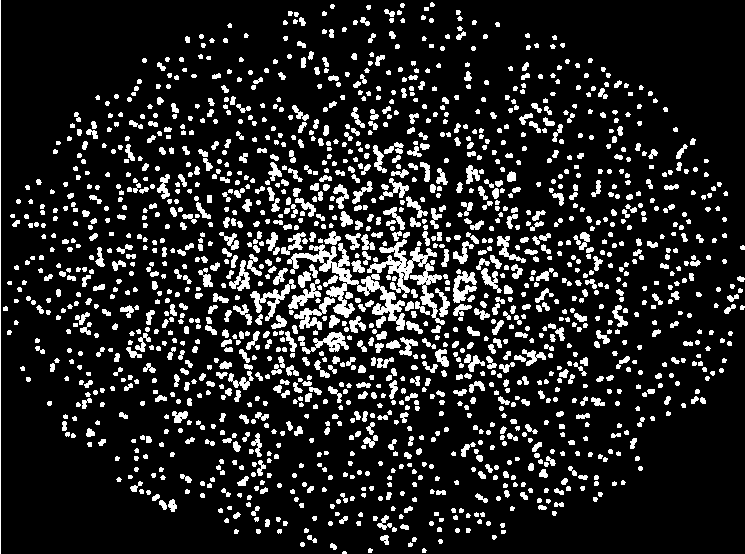
\includegraphics[width=4.1cm]{img/GCmessier_noticks_cropped.pdf}
  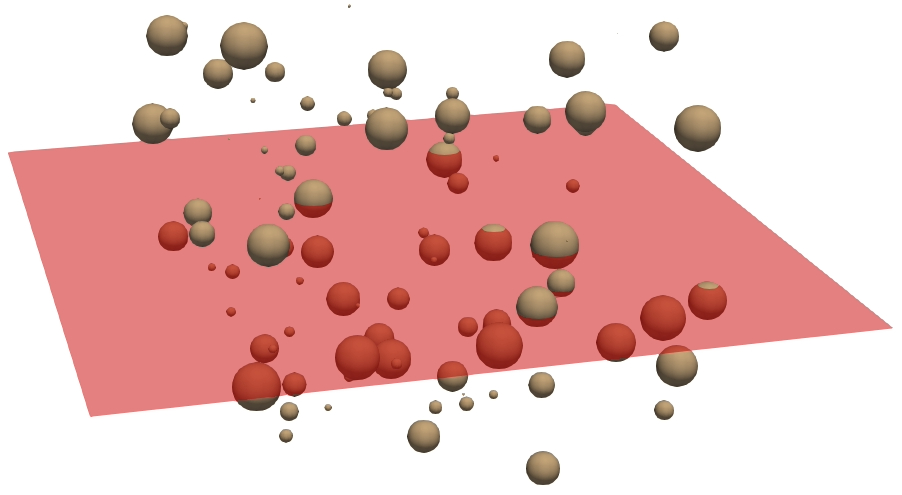
\includegraphics[width=5.1cm]{img/wicksell.jpg}
  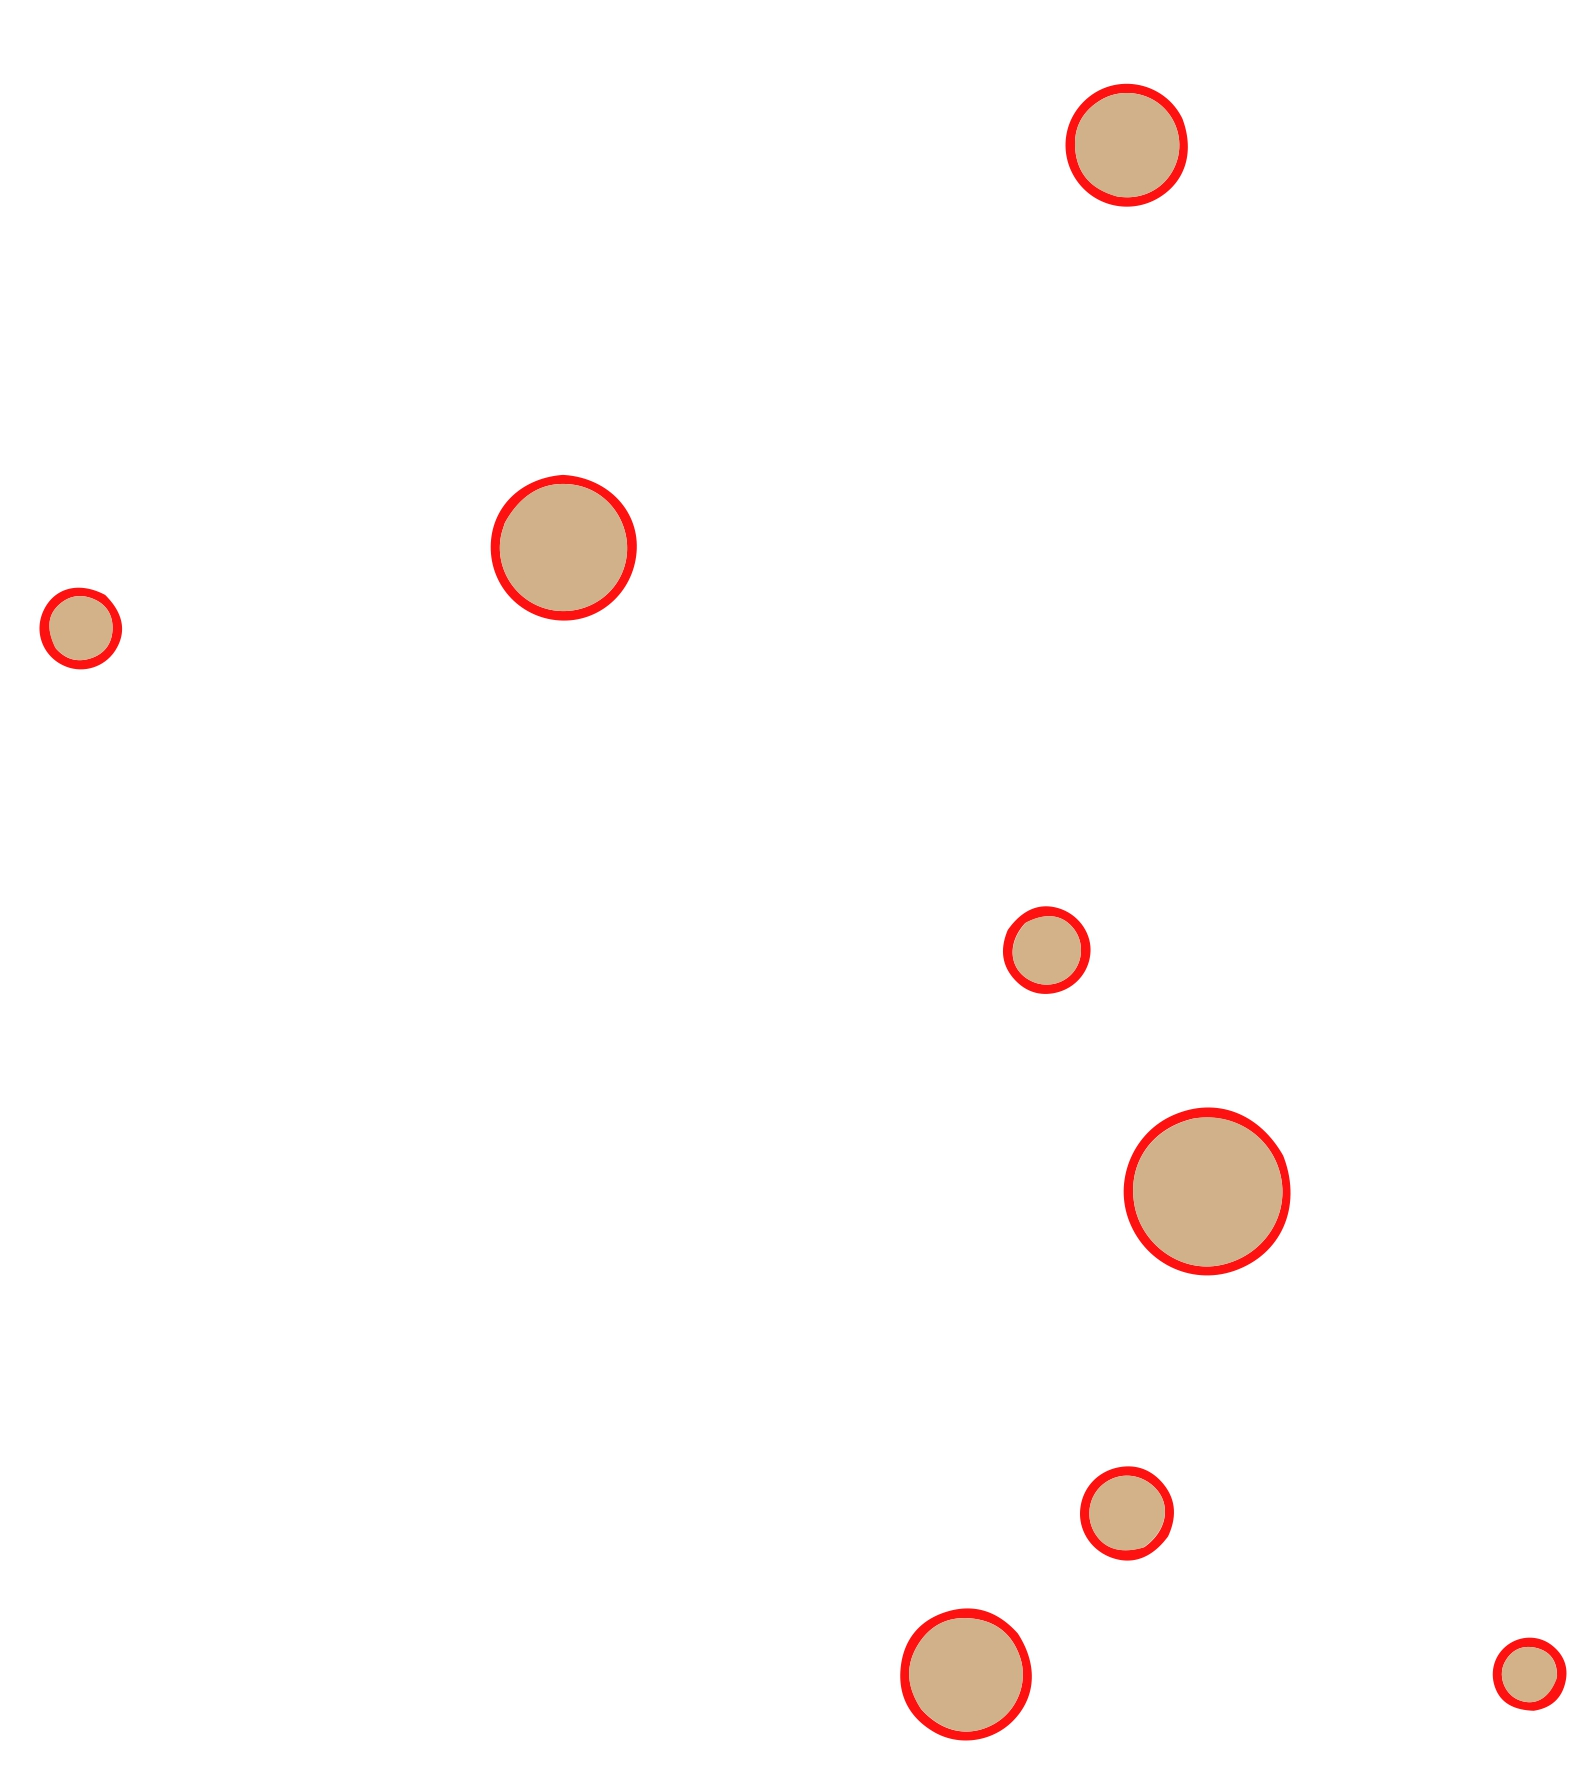
\includegraphics[width=2.7cm]{img/wick_sec_1_adobe_express_page.jpg}
  \setlength{\belowcaptionskip}{-4pt}
  \caption{Two examples of sampling in stereological inverse problems. Left panel: The Messier 4 (also designated NGC 6121) is a globular cluster in the constellation of Scorpius. Center and right panel: simulation 3D configuration with spheres and the intersecting plane in material microstructures (from \cite{27}).}\label{fig: 1 sampling}
\end{figure}

Despite their seemingly distant nature, both of these problems share a common thread: the inherent structure of an inverse problem, originally conceptualized by Wicksell (cf.\ \cite{27,1,14,15}). There, the setting of the opaque material having globular microstructure is formalized by assuming the embedded particles' radii are i.i.d.\ realization from a random variable $X^* \sim F^*$ and our observations consist of cross sections of the medium (i.e.\ "planes cutting the medium"). 

To formalize further the model note first the following two aspects: the observable radii in the cross sections cannot exceed the radii of the associated sphere; the spheres with bigger radii are more likely to be sampled. From this follows that the distribution of the squared radii of the spheres actually cut is not $F^*$ but a biased version of it; thus we write for the squared radius of the sphere actually cut: $X \sim F$. Since we assume that the samples are gathered uniformly, by Pythagoras Theorem, the observable squared circle radius $Z$ is related to $X$ via: $ Z = (1-U^2) X = Y X,$ where $U \sim U[0,1]$ and $Y \sim \operatorname{Be}(1,1/2)$. In the astronomical application, let $\mathbf{Z}= (Z_{p_1}, Z_{p_2},Z_{p_3})$ be a spherically symmetric random vector (the three-dimensional position of a star in a galaxy) of which only $(Z_{p_1}, Z_{p_2})$ can be observed. Under the assumption that the joint of $\mathbf{Z}$ is a function of the distance to the center of the galaxy, astronomers are interested in estimating the distribution of the squared distance of a star to the center of the globular cluster or galaxy $X = Z^2_{p_1}+ Z^2_{p_2}+Z^2_{p_3} \sim F$ using $Z = Z^2_{p_1}+ Z^2_{p_2} \sim G$. 

From \cite{1} and \cite{19}, it follows that both for the application in materials science and the one in astronomy, the density of the observable squared circle radii $Z \sim G$ is:
\begin{align}\label{eq: density of the observations}
g(z)=\frac{1}{2 m_0} \int_{z}^{\infty} \frac{d F^*(x)}{\sqrt{x-z}} \quad \left(= \int_{z}^{\infty} \frac{dF(x)}{2\sqrt{x^2 - xz}} \right),    
\end{align}
where $ 0 < m_0=\int_0^{\infty} \sqrt{y} \, d F^*(y) < \infty$ is the expected sphere radius under $F^*$. We can invert the above expression and obtain for $x >0$:
\begin{align*}
  & F^*(x) = 1 - \frac{V(x)}{V(0)}, \quad \quad \text{and} \quad \quad   F(x) = 1 + \frac{2}{\pi} \int_{x}^{\infty} \sqrt{s} \, dV(s) \numberthis \label{eq: solution range equation*}
\end{align*}
where, for all $x \geq 0$:
\begin{align}\label{eq: V_0 chapter2}
    V(x) \vcentcolon=\int_x^{\infty} \frac{g(z)}{\sqrt{z-x}} \: d z \quad \left(= \int_{x}^{\infty} \frac{\pi}{2 \sqrt{s}} \, dF(s)\right) 
\end{align}
and $F^*(x) = 0$ for all $x \leq 0$.  In the following sections, we will often focus on the estimation of $V$, being the common denominator for the estimation of both $F$ and $F^*$. We will also show formally how asymptotic results for the estimation of $V$ carry on to the estimation of $F^*$. Finally it is also possible to see that asymptotic results for the estimation of $V$ at $x$ carry on to the estimation of $F$ due to the following inverse formula (c.f.\ \cite{19}): 
$$
F(x) = \frac{2}{\pi} \int_0^{\infty}\sin^{-1} \left\{ \sqrt{\frac{x \wedge z}{z}} \right\} g(z)\, d z - \frac{2}{\pi} \sqrt{x} \,V(x),
$$
where the functional $\int_0^{\infty}\sin ^{-1} \sqrt{\frac{x \wedge z}{z}} g(z)\, d z$ is generally estimable at a faster rate than $V$, as its variance is finite.

\section{Adaptive and Efficient Isotonic Estimation}

Given a sample $Z_1, \ldots, Z_n$ from the density $g$ and for $\mathbb{G}_n$ the empirical distribution function based on this sample, a naive (empirical plug-in) estimator of $V$ is:
\begin{align}\label{eq: naive estimator of V chapter2}
    V_n(x) \vcentcolon=\int_x^{\infty} \frac{d\mathbb{G}_n(z)}{\sqrt{z-x}}.
\end{align}
The estimator for $F^*$ is then defined by $F^*_n(x) = 1- V_n(x)/V_n(0)$. As a function of $x$, this estimator has some undesirable properties, being non-monotone and having infinite discontinuities at a set of points becoming dense in the support of the density $g$ as $n \rightarrow \infty$. This led in \cite{1} to the definition of the so-called "isotonic inverse estimator" (IIE) $\hat{F}^*_n$ for $F^*$, which is obtained by replacing $V_n$ by its isotonic projection. This can be calculated as the right continuous derivative of the least concave majorant of the primitive function of $V_n$, which is:
$$
U_n(x)=\int_0^x V_n(y) \, dy=2 \int_0^{\infty} \sqrt{z} \, d\mathbb{G}_n(z)-2 \int_x^{\infty} \sqrt{z-x} \, d \mathbb{G}_n(z).
$$
Note that $x \mapsto U(x) = \int_{0}^x V(y) \, dy$ is a concave and increasing function on $[0,\infty)$, whereas $U_n$ is not. Taking the least concave majorant of $U_n$ on $[0,\infty)$ yields an increasing concave function. Denote by $\hat{V}_n$ the right derivative of this least concave majorant of $U_n$, and note that this will be a decreasing function on $[0,\infty)$. Then $\hat{F}^*_n$ is given by: 
\begin{align}\label{eq: isotonic estimator of F}
\hat{F}^*_n(x) := 1 - \hat{V}_n(x)/\hat{V}_n(0).
\end{align}
This estimator has the important properties of being monotone (see Figure \ref{fig: estimator performance}), right-continuous and, away from the boundary point $0$, does not depend on tuning parameters, unlike other estimators in the literature (cf.\ \cite{10}). Since $0$ is a boundary point, in the asymptotic results below $\hat{V}_n(0)$ in \eqref{eq: isotonic estimator of F} is replaced by $\hat{V}_n(x_n)$ for a sequence $x_n \downarrow 0$ (see Theorem \ref{thm: normality Holder}) and, if $F^*$ is constant around $0$, by $\hat{V}_n(y)$ for a fixed $y$ in the interior of $K_0$ (see Theorem \ref{thm: main thm iso 2}).

\begin{figure}[H]
  \vspace{-0.2cm}
  \centering
  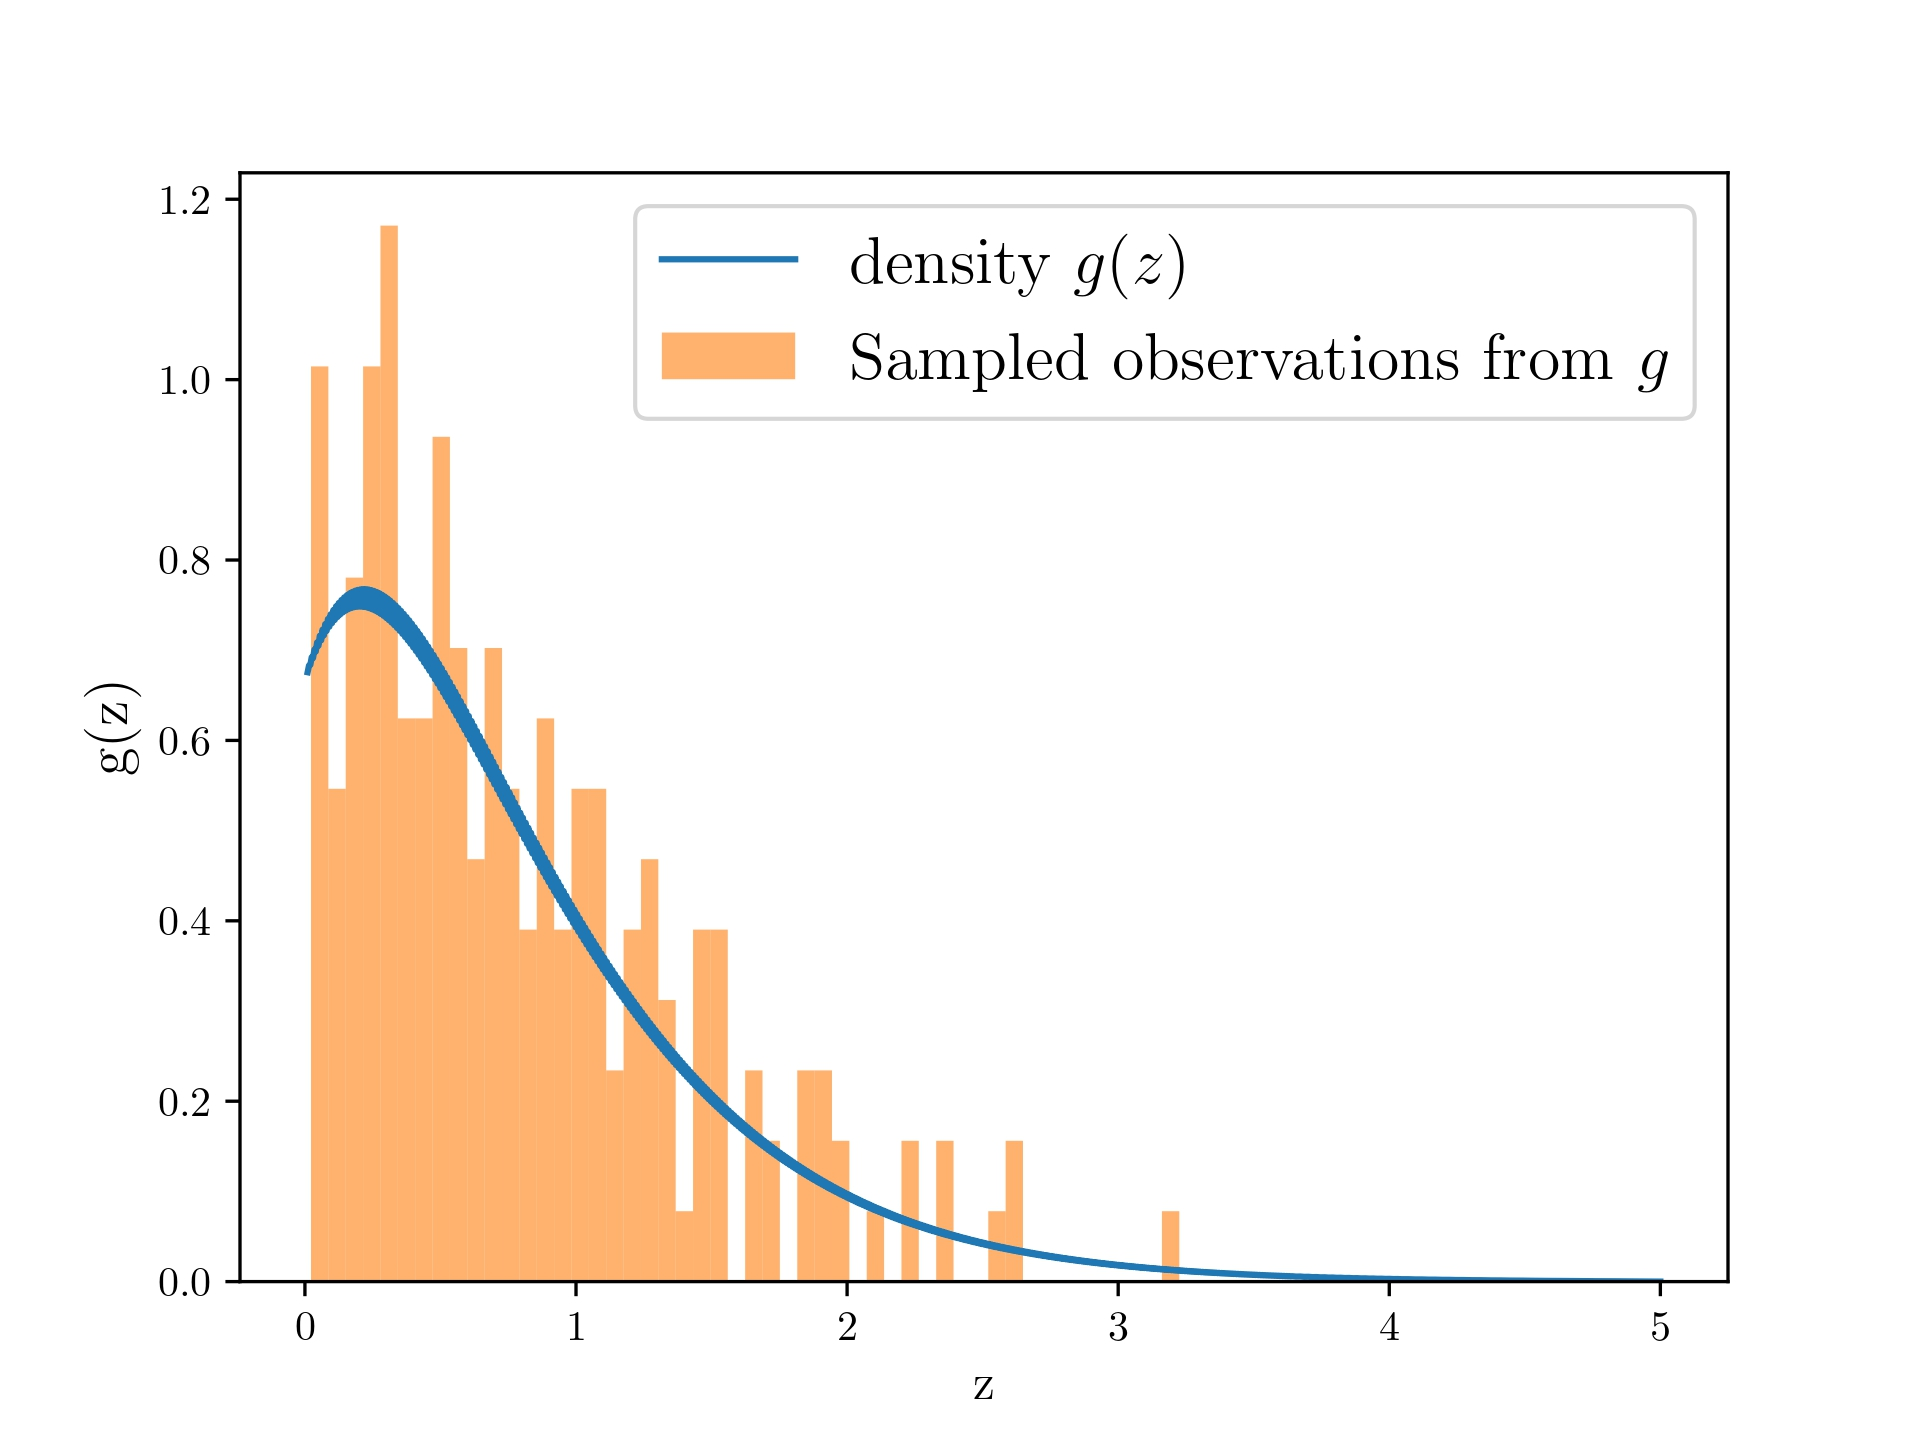
\includegraphics[width = 6cm]{img/density_new_page.jpg}
  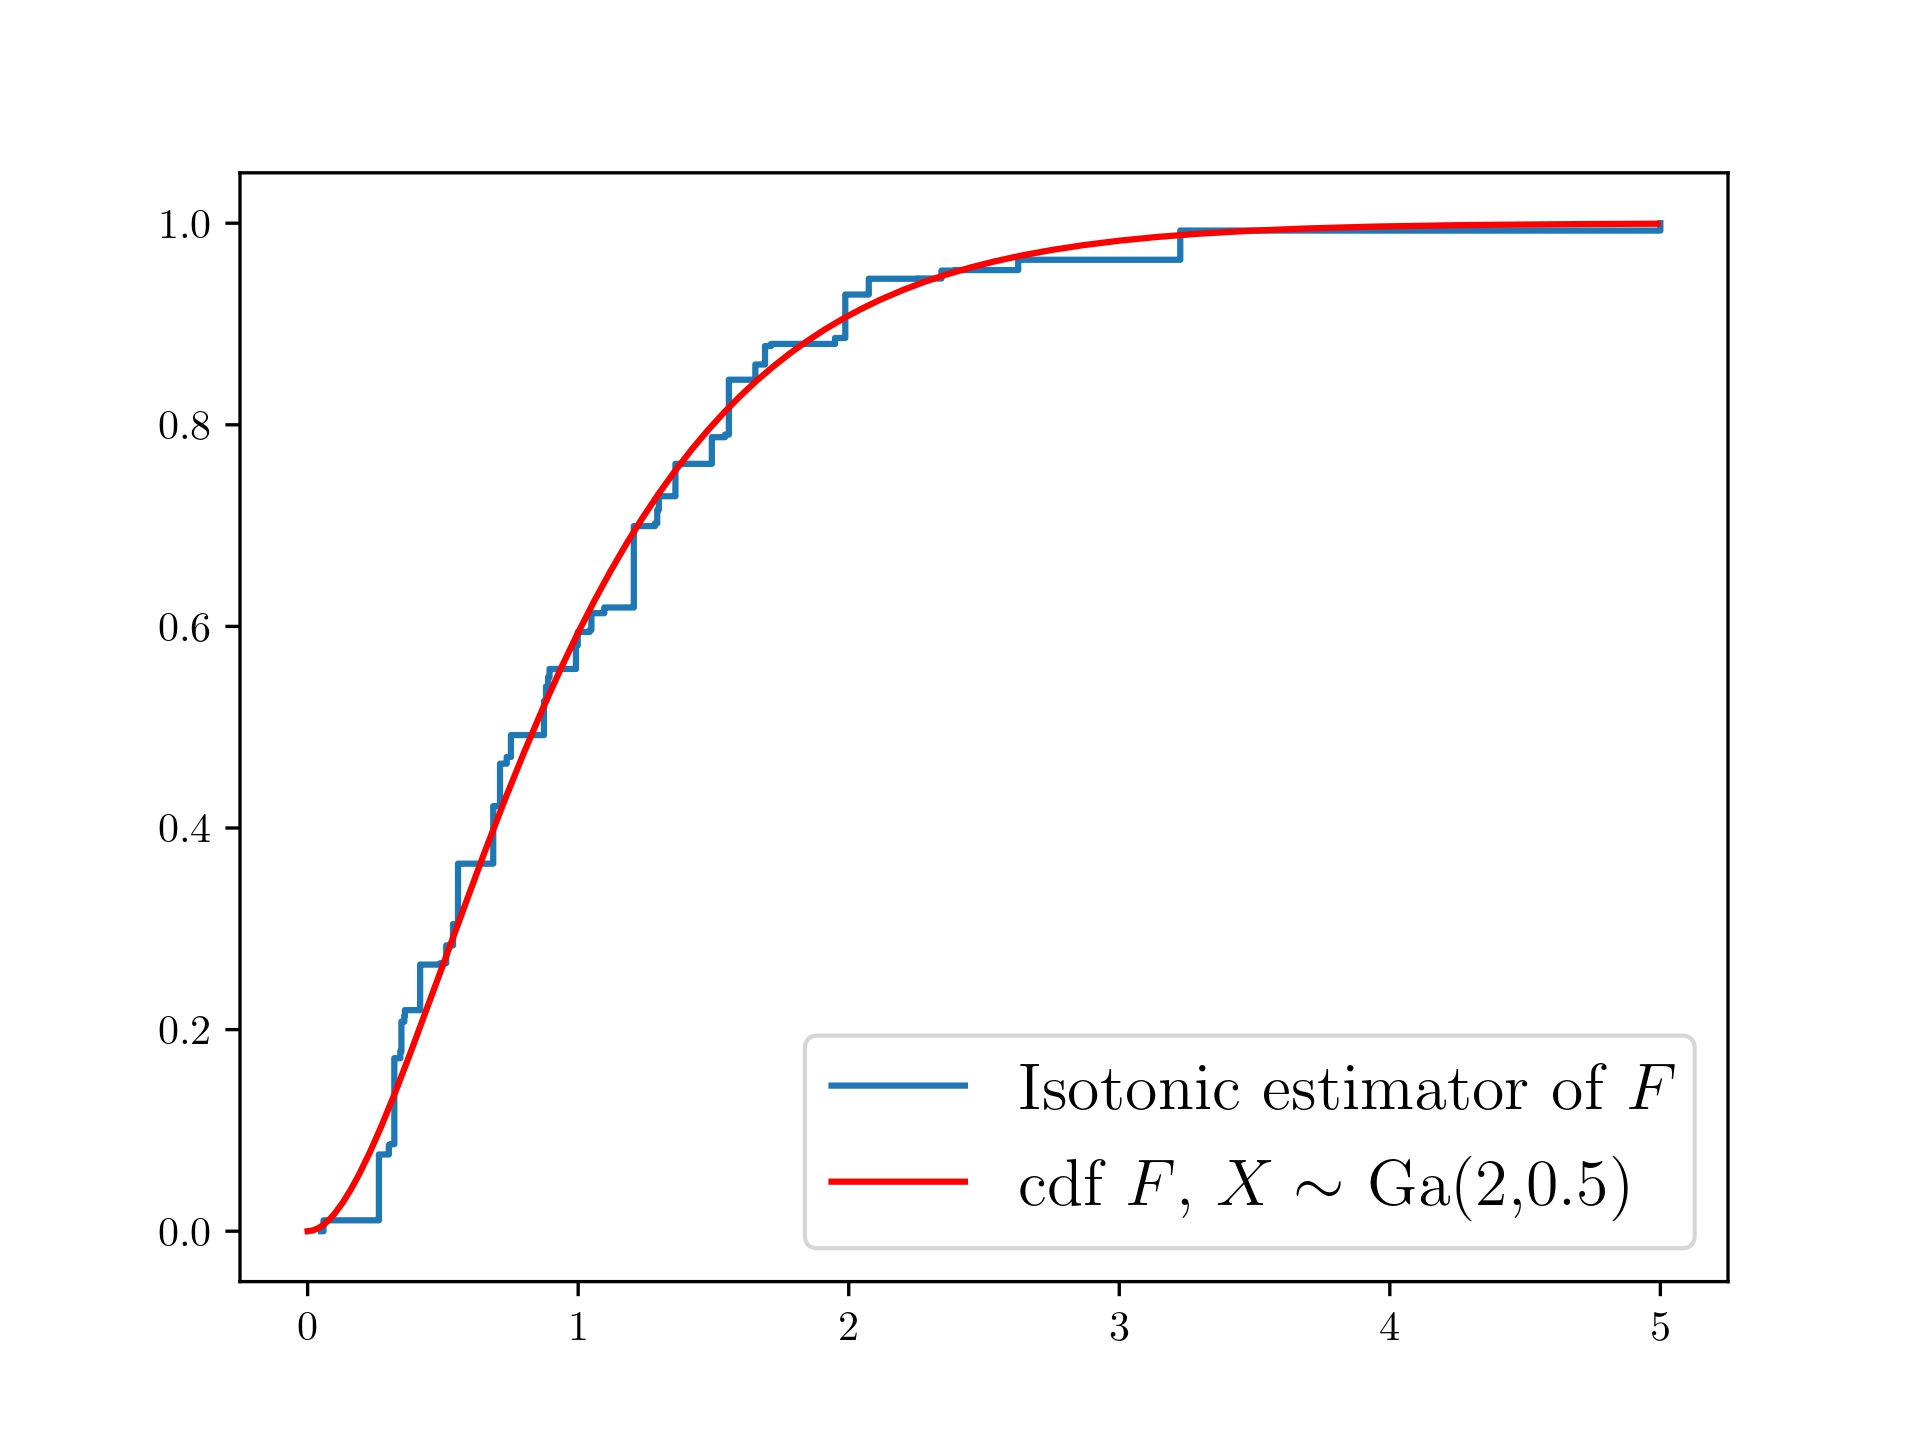
\includegraphics[width = 6cm]{img/estimator_new_page.jpg}
  \setlength{\abovecaptionskip}{-4pt}
  \setlength{\belowcaptionskip}{-8
  pt}
  \caption{200 observed draws from $g$ and isotonic estimator for $F \sim \operatorname{Ga}(2,0.5)$.}\label{fig: estimator performance}
\end{figure}

The work in this section is closely related to \cite{10} and \cite{1}. In \cite{1}, the authors observed a peculiar behavior of the isotonic estimator (IIE) compared to the naive estimator \( F^*_n(x) = 1- V_n(x)/V_n(0) \). Both estimators exhibit the same rate of estimation, \((\log{n})^{-1/2}\sqrt{n}\), and normal limiting behavior. However, the naive estimator's asymptotic variance \(\sigma^2(F^*) = \frac{4m^2_0}{\pi^2}(g(x) + g(0)(1-F^*(x))^2)\) is exactly twice that of the IIE. The authors of \cite{10} propose an explanation, showing that for \( F^* \) in the Hölder class \(\Lambda_\gamma\) with \(\gamma > \frac{1}{2}\), any efficient estimator attains the variance \(\sigma^2(F^*)/(2\gamma)\). In \cite{1}, it is assumed that \(F^*\) has a bounded density \(f\), which corresponds to \(\gamma = 1\), thus explaining the variance reduction by half.

Moreover, the authors of \cite{10} propose an estimator based on Kernel Density Estimation (KDE) that achieves the variance \(\sigma^2(F^*)/(2\gamma)\) and which is, to the best of our knowledge, the only other efficient estimator in the literature. However, the estimator they propose depends directly on the degree $\gamma$ of smoothness, which should be guesstimated before using the estimator, making it non-adaptive. Furthermore, under local conditions at $x$ and $0$ (cf. (24) and (25)), they derive an asymptotic minimax lower bound assuming $F$ is in the Hölder class $\Lambda_\gamma$, for $\gamma> \frac{1}{2}$. 

This section has two main contributions. On the one hand, we show that the IIE \(\hat{F}^*_n\) automatically adapts to the \textit{local} smoothness of \(F^*\) at \(x\), without requiring \(F^*\) to belong to a \textit{global} Hölder class. It suffices to consider the \textit{local} smoothness at points \(x\) and \(0\), measured by constants \(\gamma_x > \frac{1}{2}\) and \(\gamma_0 > \frac{1}{2}\) (see conditions \eqref{eq: condition roughness intro} and \eqref{eq: condition roughness infimum}). These can be interpreted as the tight degree of Hölder smoothness at the points $x$ and $0$. For $F^*$ with density $f$ (i.e.\ differentiable at $x$ and $0$) we retrieve the $\gamma_x = \gamma_0 = 1$ that explains the behavior observed in \cite{1}. On the other hand, we prove a lower bound on the minimax risk for any estimator sequence. The minimax theorem holds as well under local conditions of smoothness of $F^*$ around $x$ and $0$. If all conditions are met, this shows that the isotonic estimator is asymptotically efficient. No other estimator in the literature simultaneously has these properties. Consequently, the IIE emerges as the unequivocal choice, surpassing alternative estimators previously proposed in Wicksell's problem. 

First, we prove that the IIE is asymptotically normal and the smoother the cdf $F^*$ is at $x$ and $0$, the smaller the asymptotic variance automatically attained by the IIE (Theorem  \ref{thm: main thm iso 1}). Here, the smoothness of $F^*$ at a point $p$ is measured by considering constants $K_p >0$ and $\gamma_p > \frac{1}{2}$ such that:
\begin{align*}
    & \quad H_{p}(\delta ) \vcentcolon = \int_{0}^{1} \left( F^*(p+u\delta)-F^*(p) \right) \, du \sim \operatorname{sgn}(\delta) |\delta|^{\gamma_p} K_p, \quad \quad \text{as} \: \delta \rightarrow 0. \numberthis \label{eq: condition roughness intro} 
\end{align*}
Note that for $p=0$ we can only allow $\delta >0$, because $\delta <0$ would lead to $K_0 = 0$.

The adaptivity extends also to the situation where $F^*$ is constant around $x$ and $0$. Then a faster $\sqrt{n}$-rate of convergence is attained (Theorem \ref{thm: main thm iso 2}). Note that previously there were no results in the literature for nonparametric estimators that attained $\sqrt{n}$-rate in Wicksell's problem. In the case in which $F^*$ is constant only around $x$ but not around $0$, or vice versa, the rate will be again $ (\log{n})^{-1/2} \, \sqrt{n}$. We now state the first main result and its \hyperlink{proof of main thm}{proof} is given in Appendix \ref{sec: appendix chapter2}. 

\begin{theorem}\label{thm: main thm iso}
Let $F^*$ be the distribution function of the squared sphere radii and $g$ the corresponding density of the squared circle radii according to \eqref{eq: density of the observations}. Assume $\int_{0}^{\infty} y^{\frac{3}{2}} \: dF^*(y)  < \infty$ and choose $x >0$. 
\begin{thmlist}
    \item If $F^*$ satisfies condition \eqref{eq: condition roughness intro} both at $0$ and at $x$ for $\gamma_0 > \frac{1}{2}$ and $\gamma_x > \frac{1}{2}$ respectively and $g(x)<\infty$ holds true, then, as $n \rightarrow \infty$: \label{thm: main thm iso 1}
    \begin{align*}
    & \sqrt{\frac{n}{\log n}}\left( \hat{F}^*_n(x)-F^*(x)\right) \rightsquigarrow N\left(0, \frac{4m^2_0}{\pi^2} \left(\frac{g(x)}{2\gamma_x} + (1-F^*(x))^2 \frac{g(0)}{2\gamma_0} \right)\right).
    \end{align*} 
    \item If $F^*$ is constant around $x$ and $0$, with $K_x$ and $K_0$ the biggest compact intervals in $[0,\infty)$ that contain $x$ and $0$, respectively, so that $F^*$ is constant, on $K_x$ and $K_0$, with $K_x \cap K_0 = \emptyset$ and $x$ in the interior of $K_x$, then, for $\hat{F}^*_n(x) := 1 - \hat{V}_n(x)/\hat{V}_n(y)$ with $y$ a fixed point in the interior of $K_0$, as $n \rightarrow \infty$: \label{thm: main thm iso 2}
    \begin{align*}
        \sqrt{n} \left( \hat{F}^*_n(x) - F^*(x) \right) \rightsquigarrow \frac{2m_0}{\pi} \Big(L_x+ (1-F^*(x))L_0 \Big), 
    \end{align*}
    where, for any $a,b \in \mathbb{R}$, the joint distribution of $L_x$ and $L_0$ is given by:
    \begin{align*}
        \pb \left( L_x \leq a, L_0 \leq b \right) = \pb \, \bigg( \argmax_{s \in K_x} \left\{ \mathbb{Z}_x(s) - a s\right\} \leq x, \argmax_{s \in K_0} \left\{ \mathbb{Z}_y(s) - b s\right\} \leq y \bigg).
    \end{align*}
    Here $\mathbb{Z}_p(s) = \mathbb{Z}(s) - \mathbb{Z}(p),$ for $s \geq 0$ and $p \in \{x,y\}$. $\mathbb{Z}$ is a continuous centered Gaussian Process with covariance structure given by:
    \begin{align}\label{eq: covariance gauss process}
        \mathrm{Cov} \left( \mathbb{Z}(t),\mathbb{Z}(s) \right) = \mathrm{Cov} \Big( 2 \big( \sqrt{\smash[b]{Z}} - \sqrt{\smash[b]{(Z_t)_{+}}} \big), 2 \big( \sqrt{\smash[b]{Z}} - \sqrt{\smash[b]{(Z_s)_{+}}} \big) \Big),
    \end{align}
    where $Z_t = Z - t$ and $Z_s = Z - s$.
\end{thmlist}
\end{theorem}
  
The second main result of this section consists of showing that the IIE is asymptotically efficient in this setting, i.e.\ the attained asymptotic variance is the smallest attainable. This kind of result is obtained by proving a minimax lower bound for any estimator sequence estimating $F^*(x)$. Here we give a weaker (but perhaps more insightful) version of this result and its \hyperlink{proof of thm 2}{proof} is given in Appendix \ref{sec: appendix chapter2}. 

\begin{theorem}\label{thm: LAM weaker}
    Let the conditions of Theorem \ref{thm: main thm iso 1} hold, assume that $F^*$ for such $\gamma_0, \gamma_x$ satisfies \eqref{eq: condition roughness infimum} and that $g$ is continuous at $x$ and $0$. Let $\ell$ be a bowl-shaped loss function, i.e., $\ell$ is non-negative, symmetric and subconvex, then for any estimator sequence $\left( F^*_n(x)\right)_{n \in \mathbb{N}}$:
    \begin{align}\label{eq: LAM simplified}
        \lim_{\delta \downarrow 0} \: \: \liminf_{n \rightarrow \infty} \, \sup_{\| F^{\prime } - F^* \|_{\infty} < \delta} \, \ex_{\scriptscriptstyle{G_{{\scaleto{F^{\prime}}{3.7pt}}}}} \, \ell\left(\sqrt{\frac{n}{\log{n}}}\left(F^*_n(x)- F^{\prime}(x)\right)\right)  \geq \ex \ell(L),
    \end{align}
where $L$ possesses the normal distribution in Theorem \ref{thm: main thm iso 1}. $G_{F^\prime}$ is the probability measure associated to the density $g$ in \eqref{eq: density of the observations} with $F^*$ replaced by $F^\prime$.
\end{theorem}
Combining the above results shows that the IIE is an easy-to-compute, adaptive (at $x$), and efficient estimator for $F^*$.

\subsection{Asymptotics of the Isotonic Inverse Estimator}

In this subsection, we prove two main theorems that will imply Theorem \ref{thm: main thm iso}. In order to prove Theorem \ref{thm: main thm iso 1}, it is enough to look at the behavior of $\hat{V}_n(x)$ and then apply the same result also to $\hat{V}_n(0)$. We now state the conditions needed for Theorem \ref{thm: main thm iso} and \ref{thm: normality Holder}. First, a natural assumption is a moment constraint for $Z$, which can be translated into a moment condition on $X^*$ (for $0 < m_0 < \infty$): 
\begin{align*}
    \quad \int_{0}^{\infty} z \, g(z) \, dz = \frac{2}{3m_0} \int_{0}^{\infty} y^{\frac{3}{2}} \: dF^*(y)  < \infty. \numberthis \label{eq: finite first moment chapter2}
\end{align*}
Additionally, for $x \geq 0$, we need our version of $g$ to be well defined, i.e.:
\begin{align*}
    \frac{1}{2m_0}\int_{x}^{\infty} \frac{dF^*(s)}{\sqrt{s - x}}  < \infty. \numberthis \label{eq: condition finite g at x chapter2}
\end{align*}
Furthermore, we measure the smoothness of $F^*$ at $x$; $\exists$ $K >0$ and $\gamma_x > \frac{1}{2}$ such that \eqref{eq: condition roughness intro} is satisfied. 

Before proving Theorem \ref{thm: main thm iso 1}, we show that condition \eqref{eq: condition roughness intro} entails the local smoothness of the distribution function $F$ by looking at the following examples \ref{example: cdf holder} and \ref{example: cdf discrete holder} below.
\begin{example}\label{example: cdf holder}
For $\gamma_x> \frac{1}{2}$ consider the class of distribution functions locally behaved as follows. Let $F^*$ be so that there exists a neighborhood $U_x$ of $x>0$ and some $K>0$:
\begin{align*}
    F^*(u) = \begin{cases}
        F^*(x) + K(u-x)^{\gamma_x}, \quad \quad \text{for} \: u \geq x, \: u \in U_x \\
        F^*(x) - K(x-u)^{\gamma_x}, \quad \quad \text{for} \: u < x, \: u \in U_x
    \end{cases}
\end{align*}
One can think of such distribution functions as tightly Hölder smooth of degree $\gamma_x$ at the point $x$. This class is of particular importance because it illustrates what type of functions we are thinking of when we derive results under smoothness conditions at the point $x$ and 0. Such functions satisfy both conditions \eqref{eq: condition roughness intro} and \eqref{eq: condition roughness 2}. Condition \eqref{eq: condition roughness 2} follows immediately. For condition \eqref{eq: condition roughness intro} note that as $|\delta| \downarrow 0$, small enough so that $[x-|\delta|, x + |\delta|] \subset U_x$:
\begin{align*}
    H_x(\delta) = \int_{0}^{1} \left( F^*(x+u\delta )-F^*(x) \right) \, du =  \operatorname{sgn}(\delta) |\delta|^{\gamma_x} K \int_{0}^{1} u^{\gamma_x} \, du + o(\delta).
\end{align*}
\end{example}

\begin{example}\label{example: cdf discrete holder}
For any $x >0$, let $\mu_x$ be the discrete probability measure given by:
\begin{align*}
    \mu_x = \frac{1}{2} \sum_{i=1}^{\infty} p_i \left( \delta_{x+t_i} + \delta_{x-t_i}\right) ,
\end{align*}
for sequences $p_i$ of probability weights and $t_i \downarrow 0$. In particular set: $p_i = \frac{6}{\pi^2} i^{-2}$ and $t_i = i^{-\frac{1}{\gamma_x}}$ where $\gamma_x> 1/2$ and $\delta_x(\cdot)$ indicates the Dirac measure at $x$. Denote by $F^*$ the associated cdf, so that, because $\gamma_x> 1/2$, we have:
\begin{align*}
    \int_{x}^{\infty} \frac{dF^*(s)}{\sqrt{s-x}} = \frac{3}{\pi^2} \sum_{i=1}^{\infty} \frac{1}{i^2}\frac{1}{\sqrt{t_i}} = \frac{3}{\pi^2} \sum_{i=1}^{\infty} \frac{1}{i^{2- \frac{1}{2\gamma_x}}} < \infty.
\end{align*}
Moreover, we have for $\delta \downarrow 0$ (similar reasonings hold also for a generic sequence $|\delta| \downarrow 0$, we consider $\delta >0$ for simplicity):
\begin{align*}
    H_x(\delta) = \int_{0}^{1} \left( F^*(x+u\delta) - F^*(x) \right) \, du = \sum_i \frac{p_i}{2} \int_{0}^{1} \ind_{t_i \leq u \delta} \, du = \sum_i \frac{p_i (\delta - t_i)_{+}}{2\delta},
\end{align*}
which means $t_i< \delta$, thus $i > \frac{1}{\delta^{\gamma_x}}$. Therefore $H_x(\delta) = \sum_{i > 1/\delta^{\gamma_x}} \frac{p_i(\delta - i^{-1/\gamma_x})}{2\delta}$. Now we prove the following fact, as $\delta \downarrow 0$ and $k \geq 2$:
\begin{align*}
    \frac{1}{(\delta^{\gamma_x})^{k-1}} \sum_{i> \frac{1}{\delta^{\gamma_x}}} \frac{1}{i^k} \stackrel{\delta \downarrow 0}{\longrightarrow} \frac{1}{k-1}
\end{align*}
This follows directly from the fact that for $\alpha \rightarrow \infty$ (e.g.\ $\alpha = 1/\delta^{\gamma_x}$) we have:
\begin{align*}
    \frac{1}{k-1} \frac{1}{(\alpha+1)^{k-1}} = \int_{\alpha + 1}^{\infty} \frac{1}{x^k} dx \leq \sum_{i > \alpha} \frac{1}{i^k} \leq \int_{\alpha-1}^{\infty} \frac{1}{x^k} dx = \frac{1}{k-1} \frac{1}{(\alpha - 1)^{k-1}}
\end{align*}
Moreover $(\alpha/(\alpha \pm 1))^{k-1} \rightarrow 1$. Therefore as $\delta \downarrow 0$ we have:
\begin{align*}
    H_x(\delta) = \frac{6}{\pi^2} \left( \sum_{i > 1/ \delta^{\gamma_x}} \frac{1}{i^2} - \frac{1}{\delta} \sum_{i > 1/ \delta^{\gamma_x}} \frac{1}{i^{2+ \frac{1}{\gamma_x}}}\right) \sim  \frac{6}{\pi^2 (1+\gamma)} \delta^{\gamma_x}.
\end{align*}
This demonstrates that the required condition for Theorem \ref{thm: normality Holder} can also be satisfied for a discrete cumulative distribution function.
\end{example}

\begin{remark}
    Example \ref{example: cdf holder} shows that \textit{tight} Hölder smoothness of degree $\gamma_x$ at the point $x$ implies \eqref{eq: condition roughness intro}. The implication in the other direction is not true as it is shown by Example \ref{example: cdf discrete holder}, where a distribution that is not Hölder continuous at $x$ satisfies \eqref{eq: condition roughness intro}. This example also shows that \eqref{eq: condition roughness intro} does not imply Hölder continuity of $F^*$ at $x$ (i.e.\ $|F^*(x+\delta) - F^*(x)| = O(|\delta|^{\gamma_x})$ as $\delta \rightarrow 0$). The condition $|F^*(x+\delta) - F^*(x)| = O(|\delta|^{\gamma_x})$ as $\delta \rightarrow 0$ is also not sufficient for Theorem \ref{thm: normality Holder} because $|F^*(x+\delta) - F^*(x)| = O(|\delta|^{\gamma_x})$ only gives information about the upper bound of the difference, but not about the lower bound, which is also needed to be tight Hölder of degree $\gamma_x$, as can be seen by inspection of the proof of Theorem \ref{thm: normality Holder}.
\end{remark}

\begin{theorem}\label{thm: normality Holder}
Let $x \geq 0$, suppose that\eqref{eq: condition roughness intro}, \eqref{eq: finite first moment chapter2}, and\eqref{eq: condition finite g at x chapter2} hold true and $g(x)$ is given by \eqref{eq: density of the observations}. Then:
\begin{align*}
    \sqrt{\frac{n}{\log n}}\left(\hat{V}_n(x)-V(x)\right) \rightsquigarrow N\left(0, \frac{1}{2 \gamma_x} g(x)\right) \quad \text { as } n \rightarrow \infty \text {,}
\end{align*}
where, for $x=0$, we define $\hat{V}_n(0) := \hat{V}_n(x_n)$ for a sequence $x_n = o\big((n/\log n)^{-1/(2\gamma_0)}\big)$ such that $\log(1/x_n) \sim \frac{1}{2\gamma_0}\log n$ (e.g.\ $x_n = (n/\log n)^{-1/(2\gamma_0)}/\log n$).
\end{theorem}
\begin{proof}
We generalize the proof of \cite{1}, for $\gamma_x\neq 1$.

First note that \eqref{eq: condition roughness intro}, implies that $F^*$ is not constant in a neighborhood of $x$ (c.f.\ Lemma \ref{lemma: finite g if rough 2}). 
Fix $x \geq 0$ such that $x$ satisfies the conditions stated above. Define, for $a>0$, the process $T_n$ as follows:
$$
T_n(a)=\inf \left\{t \geq 0: U_n(t)-a t \text { is maximal }\right\}.
$$


The relation between $T_n$ and $\hat{V}_n$ is given by the switch relation (see \cite{2}):
\begin{align}\label{eq: switch relation}
T_n(a) \leq t \quad \Leftrightarrow \quad \hat{V}_n(t) \leq a .
\end{align}
From this relation (Lemma 3.2, \cite{2}), it follows that for each vanishing sequence $\left(\delta_n\right)$ of positive numbers, for $a\in \mathbb{R}$, for $\delta^*_n = \delta_n^{1/\gamma_x}$ ($\gamma_x$ as in \eqref{eq: condition roughness intro}), and all $n$ sufficiently large:
\begin{align*}
\delta_n^{-1}\left(\hat{V}_n(x)-V(x)\right) \leq a \: \: \: \: \: &\Leftrightarrow \: \: \: \: \: \delta_n^{-1}\left(T_n\left(a_0+\delta_n a\right)-x\right) \leq 0 \: \: \: \: \: \\
&\Leftrightarrow \: \: \: \: \: (\delta^*_n)^{-1}\left(T_n\left(a_0+\delta_n a\right)-x\right) \leq 0. 
\end{align*}
We aim to study the probability of the event on the left-hand side. We write $a_0$ for $V(x)$, which is fixed. The introduction of $\delta^*_n = \delta_n^{1/\gamma_x}$ is one of the main steps that differentiates the current proof from the one in \cite{1}. Now denote by:
$$
I_x := \begin{cases}{[0, \infty),} & \text { if } x=0 \\ \mathbb{R}, & \text { if } x>0\end{cases}
$$
\color{black} Define the localized process $\tilde{Z}_n$ in $C\left(I_x\right)$, the space of continuous functions on $I_x$, as follows (recall $a_0 = V(x)$):
$$
\tilde{Z}_n(t)=\delta_n^{-1} (\delta^*_n)^{-1} \left[U_n\left(x+\delta^*_n t\right)-U_n(x)-a_0 \delta^*_n t\right] .
$$
For each fixed $a \in \mathbb{R}$ we can, for all $n$ sufficiently large, write 
$$
\begin{aligned}
& (\delta^*_n)^{-1}\left(T_n\left(a_0+\delta_n a\right)-x\right) \\
&\quad = (\delta^*_n)^{-1} \big(\operatorname { i n f } \big\{x+t \geq 0: U_n(x+t)-a_0 x +\\
&\quad \quad \quad \quad \quad \quad \quad \quad \quad \quad \quad \quad -a_0 t-\delta_n a x-\delta_n a t \text { is maximal }\big\}-x\big) \\
&\quad = (\delta_n^*)^{-1} \inf \left\{t \geq-x: U_n(x+t)-U_n(x)-a_0 t-\delta_n a t \text { is maximal }\right\} \\
&\quad = \inf \left\{t \geq-(\delta^*_n)^{-1} x: U_n\left(x+\delta^*_n t\right)-U_n(x)-a_0 \delta^*_n t-\delta_n \delta^*_n a t \text { is maximal }\right\} \\
&\quad = \inf \left\{t \geq-(\delta^*_n)^{-1} x: \tilde{Z}_n(t)-a t \text { is maximal }\right\} ,
\end{aligned}
$$
where we use that the location of a maximum of a function is equivariant under translations and invariant under multiplication by a positive number and addition of a constant. Thus we analyze the asymptotic behavior of the process:
\begin{align*}
    \tilde{Z}_n(t)-a t =& \: \delta_n^{-1} ( \delta^*_n)^{-1} \left\{U_n\left(x+\delta^*_n t\right)-U_n(x)- U\left(x+\delta^*_n t\right)+U(x)\right\} \color{black}+ \numberthis \label{eq: rewrite Z tilde 1}\\ 
    &+ \delta_n^{-1} ( \delta^*_n)^{-1}  \left\{ U\left(x+\delta^*_n t\right)-U(x)-V(x)\delta^*_n t \right\} - at. \numberthis \label{eq: rewrite Z tilde}
\end{align*}
We will now analyze the behavior of the stochastic and deterministic terms \eqref{eq: rewrite Z tilde 1} and \eqref{eq: rewrite Z tilde} separately. Let us start with \eqref{eq: rewrite Z tilde}. The Taylor expansion of $U$ with integral form of the remainder yields:
\begin{align*}
    U(x + \delta^*_n t) - U(x) - V(x) \delta^*_n t &= \delta^*_n t \int_{0}^{1} V(x + u \delta^*_n t) - V(x) \, du \\
    &= -\frac{\delta^*_n t \pi}{2 m_0} \int_{0}^{1} F^*(x + u \delta^*_n t) - F^*(x) \, du.
\end{align*}
When we look at the limit of $\tilde{Z}_n(t) - at$ we multiply the above expression by $ \delta_n^{-1} (\delta^*_n)^{-1}= (\delta^*_n)^{-\gamma_x- 1}$. Therefore we have to look at the limit behavior of:
\begin{align}\label{eq: reasoning asympt holder}
 - (\delta^*_n)^{-\gamma_x- 1} \frac{\delta^*_n t \pi}{2 m_0} \int_{0}^{1} F^*(x + u \delta^*_n t) - F^*(x) \, du = -\frac{ |t|^{\gamma_x+ 1} \pi}{2 m_0} (K_x + o(1)),
\end{align}
where we use assumption \eqref{eq: condition roughness intro}. 

Now we consider \eqref{eq: rewrite Z tilde 1}. Defining the processes $\left(Z_n\right)$ in $C\left(I_x\right)$ as
\begin{align*}
Z_n(t) &= \delta_n^{-1} ( \delta^*_n)^{-1} \left\{U_n\left(x+\delta^*_n t\right)-U_n(x)- U\left(x+\delta^*_n t\right)+U(x)\right\} \numberthis \label{eq: Z_n(1)} \\
&=2 \delta_n^{-1} (\delta^*_n)^{-1} \int\left\{\sqrt{z-x} \ind_{[x, \infty)}(z)-\sqrt{z-x-\delta^*_n t} \ind_{\left[x+\delta^*_n t, \infty\right)}(z)\right\} \, d\left(\mathbb{G}_n-G\right)(z)
\end{align*}
we will now establish convergence in distribution of the process $Z_n$. In order to do so, we need that $g(x) < \infty$. This follows directly from \eqref{eq: condition finite g at x chapter2}. Moreover, we need the asymptotic covariance structure of the process $Z_n$, which is given by:
\begin{align}\label{eq: covariance structure final}
\operatorname{Cov}\left(Z_n(s), Z_n(t)\right)=\frac{1}{2 \gamma_x} g(x) s t\left(1-\frac{\log \log n}{\log n}\right)+O\left(\frac{1}{\log n}\right) \text {, }
\end{align}
for each fixed $s, t \in I_x$, provided that $\delta_n=n^{-1 / 2} \sqrt{\log n}$.
Therefore, using \eqref{eq: covariance structure final} and the Lindeberg-Feller Central Limit theorem we have that: 
\begin{align}\label{eq: marginal convergence chapter2}
    Z_n(1) \rightsquigarrow N(0,g(x)/(2\gamma_x)),
\end{align} 
(the \hyperlink{proof of lemma 1}{proof} of \eqref{eq: covariance structure final} and the \hyperlink{proof of lemma 2}{proof} of \eqref{eq: marginal convergence chapter2} are provided in Appendix \ref{sec: appendix chapter2}). On the other hand, by Chebyshev's inequality and \eqref{eq: covariance structure final}, we have, $\forall \: \varepsilon >0$:
\begin{align*}
    \pb\left( | Z_n (t) - t Z_n (1) | > \varepsilon \right) \leq &\frac{\mathrm{Var} ( Z_n (t) - t Z_n (1))}{\varepsilon^2} \rightarrow 0.
\end{align*}
Therefore, the finite-dimensional distributions of $Z_n$ converge weakly to the finite-dimensional distributions of the process: $ Z(t) = tX,$ in $C(I_x)$, where $X \sim N(0,g(x)/(2\gamma_x))$. We now need a stochastic equicontinuity condition to apply Theorem 2.3 from \cite{12}. Take the class of functions for $\varepsilon >0, \: M>0$:  
\begin{align*}
\mathscr{F}_{n, \varepsilon}^M=\big\{\sqrt{z-x-\delta^*_n t} & \ind_{\left[x+\delta^*_n t, \infty\right)}(z)-\sqrt{z-x-\delta^*_n s} \ind_{\left[x+\delta^*_n s, \infty\right)}(z) :  \numberthis \label{eq: class of functions chapter2} \\
&: \: s, t \in I_x,|s-t|<\varepsilon, \max (|s|,|t|)<M\big\}.
\end{align*}
This class has square integrable natural envelope $H_\varepsilon $ that satisfies for all $\varepsilon>0$ small (cf.\ Lemma \ref{lemma: variance without assum. g}): $\int H^2_{\varepsilon} (z) g (z) dz \leq g(x + \delta^*_n s \wedge t) \left( \varepsilon \delta^*_n\right)^2 \log{\frac{1}{(\varepsilon \delta^*_n)^2}}$ (as proved in Lemma \ref{lemma: conv weak argmax} this class of functions is also VC).
Therefore, by using maximal inequality 3.1 (ii) from 
\cite{12} we obtain:
\begin{align*}
    &\limsup_{n \rightarrow \infty}\pb \left\{ \sup_{\mathscr{F}_{n, \varepsilon}^M} |Z_n(s) - Z_n(t)| > \eta \right\} \leq \limsup_{n \rightarrow \infty} \frac{\ex \sup_{\mathscr{F}_{n, \varepsilon}^M} |Z_n(s) - Z_n(t)|^2 }{\eta^2} \\
    &\leq \limsup_{n \rightarrow \infty} \, \frac{J(1)^2 g(x + \delta^*_n s \wedge t)}{(\delta^*_n)^2 \log{n}} (\varepsilon \delta^*_n)^2 \log{(\varepsilon \delta^*_n)^{-2}} =  J(1)^2 \gamma_x^{-1} \eta^{-2} g(x) \varepsilon^2 \stackrel{\varepsilon \rightarrow 0}{\longrightarrow} 0.
\end{align*}
where the reason why the uniform entropy integral is finite is as in the proof of Lemma \ref{lemma: conv weak argmax}.
The stochastic equicontinuity condition, together with the convergence in distribution of the finite-dimensional distributions, implies convergence in distribution of $Z_n$ to $Z$ in $(C(I_x),d)$ where $d$ is the metric of uniform convergence on compacta. Next, we need the stochastic boundedness of the sequence $T_n$ given below in \eqref{eq: stochastic boundedness seq argmax} (the \hyperlink{proof of lemma 3}{proof} of which is given in Appendix \ref{sec: appendix chapter2}). For $a_0 = V(x)$ and $n \rightarrow \infty$:
\begin{align}\label{eq: stochastic boundedness seq argmax}
T_n\left(a_0 + \delta_n a \right)=V^{-1}\left(a_0\right)+O_p\left(\delta^*_n\right).
\end{align}
One can now apply Theorem 2.7 from \cite{12} to the process $\tilde{Z}_n$. 
\begin{align}\label{eq: convergence argmax}
(\delta^*_n)^{-1}\left(T_n\left(a_0+\delta_n a\right)-x\right) & \rightsquigarrow \underset{t \in I_x}{\arg \max }\left\{t X-\frac{|t|^{\gamma_x+ 1} \pi}{2 m_0} K_x  -a t \right\}. 
\end{align}
But it is immediate to see that, almost surely (Lemma~\ref{lem: continuity argmax holder}):
\begin{align}\label{eq: iff relation argmax}
    \underset{t \in I_x}{\arg \max }\left\{t X-\frac{|t|^{\gamma_x+ 1} \pi}{2 m_0} K_x  -a t \right\} \leq 0 \: \: \: \: \iff \: \: \: \: X \leq a.
\end{align}
Hence, using the two relations above:
\begin{align*}
&\pb\left\{\delta_n^{-1}\left(\hat{V}_n(x)-V(x)\right) \leq a\right\}=\pb\left\{(\delta^*_n)^{-1}\left(T_n\left(a_0+\delta_n a\right)-x\right) \leq 0\right\} \stackrel{n \rightarrow \infty}{\longrightarrow} \\
& \quad \stackrel{\eqref{eq: convergence argmax}}{\longrightarrow} \pb \left\{ \underset{t \in I_x}{\arg \max }\left\{t X-\frac{|t|^{\gamma_x+ 1} \pi}{2 m_0} K_x  -a t \right\} \leq 0 \right\} \stackrel{\eqref{eq: iff relation argmax} }{=} \pb\{ X \leq a\},
\end{align*}
where the convergence holds because, for $x>0$, $0$ is a continuity point of the limit distribution in \eqref{eq: convergence argmax} (Lemma~\ref{lem: continuity argmax holder}). This proves the theorem for $x>0$.

For $x=0$ since $I_0=[0,\infty)$, the limit in \eqref{eq: convergence argmax} has an atom at $0$ of mass $\pb\{X \leq a\}$. This is why $\hat{V}_n$ is evaluated at $x_n$. Write $\hat{s}_n := (\delta^*_n)^{-1} T_n(a_0+\delta_n a)$ and $\kappa_n := x_n/\delta^*_n$, so that $\kappa_n \rightarrow 0$ and $\log(1/\kappa_n) = o(\log n)$ by the assumptions on $x_n$. By the switch relation \eqref{eq: switch relation}:
\begin{align*}
\pb\left\{\delta_n^{-1}\left(\hat{V}_n(0)-V(0)\right) \leq a\right\} = \pb\left\{\hat{V}_n(x_n) \leq a_0+\delta_n a\right\} = \pb\left\{T_n(a_0+\delta_n a) \leq x_n\right\} = \pb\left\{\hat{s}_n \leq \kappa_n\right\},
\end{align*}
so it suffices to show that $\pb\{\hat{s}_n \leq \kappa_n\} \rightarrow \pb\{X \leq a\}$. At $x=0$ the limit in \eqref{eq: convergence argmax} is, with $c := \pi K_0/(2m_0)$:
\begin{align*}
\hat{s} := \underset{t \geq 0}{\arg\max}\left\{tX - c\, t^{\gamma_0+1} - at\right\} = \left(\frac{(X-a)_+}{c(1+\gamma_0)}\right)^{1/\gamma_0}.
\end{align*}
Fix $\varepsilon>0$. For $n$ large we have $\kappa_n \leq \varepsilon$ and, since $[0,\varepsilon]$ is closed in $I_0$, the portmanteau lemma gives:
\begin{align*}
\limsup_{n \rightarrow \infty} \pb\left\{\hat{s}_n \leq \kappa_n\right\} \leq \limsup_{n \rightarrow \infty} \pb\left\{\hat{s}_n \leq \varepsilon\right\} \leq \pb\left\{\hat{s} \leq \varepsilon\right\} = \pb\left\{X \leq a + c(1+\gamma_0)\varepsilon^{\gamma_0}\right\},
\end{align*}
which tends to $\pb\{X \leq a\}$ as $\varepsilon \rightarrow 0$. For the lower bound fix $M \geq 1$ and $\eta>0$. Since $F^*$ is nondecreasing, the term in \eqref{eq: rewrite Z tilde} is at most $-at$, that is, $\tilde{Z}_n(t) \leq Z_n(t)$ for $t \geq 0$. We claim that:
\begin{align*}
\left\{Z_n(1) \leq a-\eta\right\} \cap \left\{\sup_{\kappa_n < t \leq M}\left|\frac{Z_n(t)}{t}-Z_n(1)\right| \leq \eta\right\} \cap \left\{\hat{s}_n \leq M\right\} \subseteq \left\{\hat{s}_n \leq \kappa_n\right\}.
\end{align*}
Indeed, on the event on the left-hand side we have $Z_n(t)/t \leq a$ for all $t \in (\kappa_n, M]$, and therefore
\begin{align*}
\tilde{Z}_n(t) - at \leq Z_n(t) - at \leq 0 = \tilde{Z}_n(0) \quad \text{for all } t \in (\kappa_n, M].
\end{align*}
So no point of $(\kappa_n, M]$ can be the smallest maximizer of $\tilde{Z}_n(t)-at$ (otherwise $0$ would be a maximizer smaller than it), and since $\hat{s}_n \leq M$ we get $\hat{s}_n \leq \kappa_n$. Hence:
\begin{align*}
\pb\left\{\hat{s}_n \leq \kappa_n\right\} \geq \pb\left\{Z_n(1) \leq a-\eta\right\} - \pb\left\{\sup_{\kappa_n < t \leq M}\left|\frac{Z_n(t)}{t}-Z_n(1)\right| > \eta\right\} - \pb\left\{\hat{s}_n > M\right\}.
\end{align*}
By \eqref{eq: marginal convergence chapter2} the first term converges to $\pb\{X \leq a-\eta\}$, and the second term converges to zero by Lemma~\ref{lemma: uniform collapse} (see Appendix \ref{sec: appendix chapter2}). By \eqref{eq: stochastic boundedness seq argmax} with $x=0$, $\hat{s}_n = O_p(1)$, so the last term is arbitrarily small for $M$ large, uniformly in $n$. Letting $n \rightarrow \infty$, then $M \rightarrow \infty$ and $\eta \rightarrow 0$, we obtain $\liminf_{n} \pb\{\hat{s}_n \leq \kappa_n\} \geq \pb\{X \leq a\}$, which concludes the proof for $x=0$.
\end{proof}

\begin{example}\label{example: holder + local behavior}
As in \cite{10}, it is possible to conduct the analysis in accordance with the global smoothness properties of the underlying distribution function $F^*$. Consider, for arbitrary $\gamma=\alpha+\beta, \alpha=0,1, \ldots, 0<\beta \leq 1$, the Hölder class $C^{\gamma}$ of functions $f(y), y \geq 0$ having finite norm:
\begin{align}\label{eq: holder norm definition}
\|f\|_\gamma=\sup _{y \geq 0}|f(y)|+\sup _{x, y \geq 0} \frac{\left|f^{(\alpha)}(x)-f^{(\alpha)}(y)\right|}{|x-y|^\beta}.
\end{align}
Then assume $F \in C^{\gamma}$ for $\gamma > \frac{1}{2}$. Moreover, assume:
\begin{align}\label{eq: condition roughness 2}
    \lim_{t \rightarrow 0} \frac{|F^*(x+t)-F^*(x)|}{|t|^{\gamma}} = K > 0.
\end{align}
Note that it is possible to prove that if $F^* \in C^{\gamma}$ for $\gamma > 1/2$, then the density of the observations $g$ is bounded and continuous (see Lemma \ref{lemma: bounded density}). We show that the combination of \eqref{eq: holder norm definition} and \eqref{eq: condition roughness 2} implies \eqref{eq: condition roughness intro}.
Using the Dominated Convergence Theorem in combination with the assumption of the Hölder condition, and \eqref{eq: condition roughness 2}, we obtain as $\delta \rightarrow 0$:
\begin{align}\label{eq: reasoning asympt holder 2}
 \int_{0}^{1} \frac{F^*(x + u \delta) - F^*(x)}{ \operatorname{sgn}(\delta) |\delta|^{\gamma} u^{\gamma}} u^{\gamma} \, du \rightarrow K. 
\end{align}
\end{example}

Also for the case of Theorem \ref{thm: main thm iso 2}, we look first at the behavior of $\hat{V}_n(x)$. 

\begin{theorem}\label{thm: distrib flat F at x}
    Let $x > 0$, and $K_x :=[\ubar{x},\bar{x}] \subset [0,\infty)$ the biggest interval that contains $x$ on which $F^*$ is constant, with $\ubar{x} < x < \bar{x}$. Assume that \eqref{eq: finite first moment chapter2} holds true. Then:
    \begin{align*}
        \sqrt{n} \left( \hat{V}_n(x) - V(x) \right) \rightsquigarrow L_x,
    \end{align*}
    where, for any $a \in \mathbb{R}$:
    \begin{align*}
        \pb \left( L_x \leq a \right) = \pb \left( \argmax_{s \in K_x} \left\{ \mathbb{Z}_x(s) - a s\right\} \leq x \right). 
    \end{align*}
    for $\mathbb{Z}_x$ a centered continuous Gaussian Process with covariance structure given by:
    \begin{align}
        \mathrm{Cov} \left( \mathbb{Z}_x(t),\mathbb{Z}_x(s) \right) =  \mathrm{Cov} \left( 2 \big( \sqrt{(Z_x)_{+}} - \sqrt{(Z_t)_{+}} \big), 2 \big( \sqrt{(Z_x)_{+}} - \sqrt{(Z_s)_{+}} \big) \right).
    \end{align}
    where $Z_x := Z-x$ and analogously $Z_t$ and $Z_s$.
\end{theorem}
\begin{proof}
\begin{comment}
First, for $a >0$ we have:
\begin{align*}
    & \hat{V}_n (x) \leq a \quad \Leftrightarrow \quad {\argmax_{s \geq 0}}^{-} \left\{ U_n(s) - as \right\} \leq x. 
\end{align*}
\end{comment}
Using \eqref{eq: switch relation} we obtain for each fixed $a \in \mathbb{R}$, for all $n$ sufficiently large:
\begin{align*}
    &\sqrt{n} \left( \hat{V}_n (x) - V(x) \right) \leq a \quad \\
     \quad \Leftrightarrow \quad  &\inf \big\{s \geq 0: U_n(s) - \left(V(x)+ a/\sqrt{n} \right) s \: \text { is maximal} \big\} \leq x \quad \quad \\
    \quad \Leftrightarrow \quad  &\inf \big\{s \geq 0: (U_n (s) - U_n(x) - U (s) + U(x) ) + \\
    & \quad \quad \quad \quad + (U(s) - U(x) - V(x)(s-x) ) -  (a s)/\sqrt{n}  \text { is maximal} \big\} \leq x. 
\end{align*}
where we use that the location of a maximum of a function is equivariant under translations. Now using the invariance under multiplication by a positive number and addition of a constant, and defining:
\begin{align}
    &Z_n(s) := \sqrt{n} (U_n (s) - U_n(x) - U (s) + U(x) ) \quad \text{and} 
    \\ \quad &h_x(s) := U(x) - U(s) - V(x)(x-s).
\end{align}
we obtain that the above event can be rewritten as:
\begin{align*}
    \inf \big\{s \geq 0: Z_n(s) - a s - \sqrt{n} h_x(s)  \text { is maximal} \big\} \leq x,
\end{align*}
\begin{lemma}\label{lemma: conv weak argmax}
Let $\ell^{\infty}$ be endowed with uniform norm. Define:
$$ Z^*_n(s) := \sqrt{n} \left( U_n(s) - U(s) \right) $$
then:
\begin{align}\label{eq: convergence ell^infty Z 1}
    Z^*_n \rightsquigarrow \mathbb{Z} \quad \text{in} \: \: \ell^{\infty}[0,\infty),
\end{align}    
where $\mathbb{Z}$ is a Gaussian Process with a.s. continuous sample paths relative to the Euclidean metric. In particular:
\begin{align}\label{eq: norm infinity convergence}
    \|U_n - U \|_{\infty} = \sup_{s\geq 0} |U_n(s)- U(s)| \stackrel{\pb}{\rightarrow} 0.
\end{align}
\end{lemma}
The \hyperlink{proof of lemma weak conv}{proof} of this lemma is given in Appendix \ref{sec: appendix chapter2}. Consequently:
\begin{align}\label{eq: convergence ell^infty Z}
    Z_n = Z^*_n - Z^*_n(x) \rightsquigarrow \mathbb{Z} - \mathbb{Z}(x) =: \mathbb{Z}_x \quad \text{in} \: \: \ell^{\infty}[0,\infty),
\end{align}    
where also $\mathbb{Z}_x$ is a Gaussian Process with a.s. continuous sample paths relative to the Euclidean metric. By the above computations, we conclude that the limiting behavior of: 
$$\widetilde{Z}_n (s) :=  Z_n(s) - a s - \sqrt{n} h_x(s), $$ 
is determined by the process $\mathbb{W}$ which is defined by:
$$
\mathbb{W}(s) = \begin{cases}
        \mathbb{Z}_x(s) -as, & \text{for } s \in [\ubar{x},\bar{x}]\\
        -\infty, & \text{for } s \notin [\ubar{x},\bar{x}] 
        \end{cases} 
$$
This is because: $h_{x}(s) \geq 0$ for all $s \in (0 ,\ubar{x}) \cup (\bar{x},\infty)$, and therefore multiplied by $-\sqrt{n}$ will go to $-\infty$ in case the inequality is strict; however $h_x(s) = 0, \: \: \forall \: s \in [\ubar{x},\bar{x}]$ and thus on that interval the limiting behavior is completely determined by $\mathbb{Z}_x(s) -as$ (using the limiting behavior of $Z_n$ derived above). Let:
\begin{align*}
&\hat{s}_n := \inf \left\{ s \geq 0 \: : \:  Z_n(s) - a s - \sqrt{n} h_x(s)  \: \: \text{is maximal} \right\} \numberthis \label{eq: def hat{t}_n 1},\\
&\hat{s} := \argmax_{s \geq 0} \left\{\mathbb{W}(s) \right\} = \argmax_{s \in [\ubar{x},\bar{x}]} \left\{\mathbb{Z}_x(s) - as \right\}. \numberthis \label{eq: def hat{t} 1}
\end{align*}
To prove convergence in distribution we use the Portmanteau Lemma and show for every closed subset $F$ of $[0,\infty)$: $\limsup_{n \rightarrow \infty} \pb \left( \hat{s}_n \in F \right) \leq \pb \left( \hat{s} \in F \right)$. 

Let us start by choosing a sequence $\varepsilon_n \downarrow 0$ such that $\sqrt{n} h_x(\ubar{x}-\varepsilon_n) \rightarrow \infty$ and $\sqrt{n} h_x(\bar{x}+\varepsilon_n) \rightarrow \infty$. This exists since $\forall \: \varepsilon > 0$, we have $\sqrt{n} h_x(\ubar{x}-\varepsilon) \wedge h_x(\bar{x}+\varepsilon) \rightarrow \infty$. Moreover, $h_x(\bar{x}+\varepsilon)$ is an increasing function in $\varepsilon$ that has a zero in $\varepsilon =0$. The behavior is analogous for $h_x(\ubar{x}-\varepsilon)$. Therefore it is sufficient to construct a sequence of $\varepsilon_n$ such that $h_x(\ubar{x}-\varepsilon_n) \wedge h_x(\bar{x}+\varepsilon_n) = O(1/n^\alpha)$ for some $\alpha < 1/2$. 
For $K_n := [\ubar{x}-\varepsilon_n,\bar{x}+\varepsilon_n]$ and for $K := [\ubar{x},\bar{x}]$ (denoted by $K_x$ in the statement):
\begin{align*}
    &\limsup_{n \rightarrow \infty} \pb \left(\hat{s}_n \in F  \right) \leq \limsup_{n \rightarrow \infty} \pb \left(\hat{s}_n \in F \cap K_n \right) + \limsup_{n \rightarrow \infty} \pb \left(\hat{s}_n \in K^{c}_n  \right)  \\
    & \leq \underbrace{\limsup_{n \rightarrow \infty} \pb \left( \sup_{s \in F \cap K_n} \widetilde{Z}_n(s) \geq \sup_{s \in K_n} \widetilde{Z}_n(s) \right)}_{(1)} + \underbrace{\limsup_{n \rightarrow \infty} \pb \left(\hat{s}_n \in K^{c}_n  \right).}_{(2)} \numberthis \label{eq: two terms to show Portmanteau}
\end{align*}
We look at (2) in \eqref{eq: two terms to show Portmanteau} and show it goes to zero. To do this, we need relation \eqref{eq: conv K^c_n} and its \hyperlink{proof of lemma conv K^c_n}{proof} is given Appendix \ref{sec: appendix chapter2}. Thus:
\begin{align}\label{eq: conv K^c_n}
    \sup_{s \in K^c_n} \widetilde{Z}_n(s) = \sup_{s \in K^c_n}  \big\{ Z_n(s) - a s - \sqrt{n} h_x(s) \big\} \stackrel{\pb}{\rightarrow} - \infty,
\end{align}
implies that:
\begin{align*}
    \pb \left(\hat{s}_n \in K^{c}_n  \right) &\leq \pb \bigg( \sup_{s \in K^c_n} \widetilde{Z}_n(s) \geq \sup_{s \in K_n} \widetilde{Z}_n(s) \bigg) \\
    & \leq \pb \, \bigg( \sup_{s \in K^c_n} \widetilde{Z}_n(s) \geq \sup_{s \in K} \big\{ Z_n(s) -as \big\} \bigg) \rightarrow 0. \numberthis \label{eq: probabilities hat{t}_n in K^c}
\end{align*}
The last convergence is a consequence of \eqref{eq: conv K^c_n} and that $Z_n \rightsquigarrow \mathbb{Z}$ on $\ell^{\infty} (K)$, combined with the continuous mapping theorem (i.e.\ the term on the left-hand side of the inequality is $O_p(1)$).

Now we argue the behavior of (1). For that, we need an additional convergence in probability given in \eqref{eq: conv prob argmax}, and its \hyperlink{proof of lemma conv prob}{proof} is provided Appendix \ref{sec: appendix chapter2}.
\begin{align}\label{eq: conv prob argmax}
    \sup_{s \in F \cap K_n} \left\{Z_n(s) - \sqrt{n} h_x(s) -as\right\} - \sup_{s \in F \cap K} \left\{Z_n(s) -as\right\} \stackrel{\pb}{\longrightarrow} 0.
\end{align}
Using that:
\begin{align*}
    \sup_{s \in F \cap K} \left\{Z_n(s) -as\right\} \rightsquigarrow \sup_{s \in F \cap K} \left\{\mathbb{Z}_x(s) -as\right\},
\end{align*}
we conclude using Theorem 2.7 (iv) from \cite{6} and \eqref{eq: conv prob argmax}:
\begin{align*}
    \sup_{s \in F \cap K_n} \left\{Z_n(s) - \sqrt{n} h_x(s) -as\right\} \rightsquigarrow  \sup_{s \in F \cap K} \left\{\mathbb{Z}_x(s) -as\right\}.
\end{align*}
We derive the behavior of (1) in \eqref{eq: two terms to show Portmanteau}. This term can be upper bounded by:
\begin{align*}
    &\limsup \pb \left( \sup_{s \in F \cap K_n} \left\{Z_n(s) - \sqrt{n} h_x(s) -as\right\} \geq \sup_{s \in K} \left\{ Z_n(s) -as \right\} \right) \\
    &\leq \pb \left( \sup_{F \cap K} \left\{\mathbb{Z}_x(s) -as\right\} \geq \sup_{s \in K} \left\{\mathbb{Z}_x(s) -as\right\} \right) \leq \underbrace{\pb (\hat{s} \in K^c)}_{=0} + \pb \left( \hat{s} \in F \right) \numberthis \label{eq: first term portmanteau}
\end{align*}
where we used the above derivations, together with Lemma \ref{lemma: conv weak argmax} and Theorem 2.7 (v) from \cite{6}. Therefore by \eqref{eq: two terms to show Portmanteau} combined with \eqref{eq: probabilities hat{t}_n in K^c}, \eqref{eq: first term portmanteau} and Portmanteau Lemma we obtain the desired convergence in distribution, which can be restated:
\begin{align*}
    & \pb \left(\sqrt{n} \big( \hat{V}_n (x) - V(x) \big) \leq a \right) =  \pb \Big( \hspace{-0.05cm}  \inf_{s \geq 0} \big\{ Z_n(s) - a s - \sqrt{n} h_x(s)  \text { is maximal} \big\} \hspace{-0.05cm} \leq x \Big) \\
    & \stackrel{n \rightarrow \infty}{\longrightarrow}  \pb \bigg( \argmax_{s \in K} \left\{ \mathbb{Z}_x(s) - a s\right\} \leq x \bigg).
\end{align*}
Note that the last expression defines the cdf of a random variable $L_x$, which is the right derivative of the least concave majorant of the process $\mathbb{Z}_x$ evaluated at $x$. Indeed, by the switch relation and Lemma \ref{lem: lil continuity}, we have 
$\pb \left( \argmax_{s \in K} \left\{ \mathbb{Z}_x(s) - a s\right\} \leq x \right) = \pb \left( L_x \leq a \right).$
\end{proof}

Note that the \hyperlink{proof of main thm}{proof} of Theorem \ref{thm: main thm iso 1} (included in Appendix \ref{sec: appendix chapter2}) is a consequence of Slutsky's Lemma, Theorem \ref{thm: normality Holder} and \ref{thm: distrib flat F at x}, the fact that $1 - F^*(x) = V(x)/V(0)$ together with the asymptotic independence of $\hat{V}_n(x)$ and $\hat{V}_n(0)$. The proof of Theorem \ref{thm: main thm iso 2} follows the same steps, using Theorem \ref{thm: distrib flat F at x}.

\begin{remark}
Let $x>0$, and suppose that $F^*$ satisfies condition \eqref{eq: condition roughness intro} both at $x$ and at 0 for a common $\gamma_x> \frac{1}{2}$ and \eqref{eq: finite first moment chapter2} holds true. Then, by Theorem \ref{thm: main thm iso 1}:
\begin{align}
& \sqrt{\frac{n}{\log n}}\left( \hat{F}^*_n(x) -F^*(x)\right) \rightsquigarrow N\left(0, \frac{g(x) V(0)^2+g(0) V(x)^2}{2 \gamma_xV(0)^4}\right).
\end{align}
The asymptotic variance obtained here coincides with the one obtained in obtained in \cite{10} where it is given a unique $\gamma$ and the one in \cite{1} with $\gamma_x= 1$. 
\end{remark}

\subsubsection*{Simulation study limiting process Theorem \ref{thm: distrib flat F at x}}

In this subsection, we present some simulations about the distribution of $L_x$ of Theorem \ref{thm: distrib flat F at x}; in particular we show how to constructively sample from $L_x$ and that, even if $L_x$ is not normal, its behavior is close to being normal.
First, we consider an underlying distribution function $F^*$ of the squared radii as displayed in the left panel of Figure \ref{fig: 1}, which is constant on $[2,3]$; observe in light blue a histogram of $1000$ gathered samples from the associated density of the observations $g$ (note that we obtain observations also on the interval where $F^*$ is constant).

\begin{figure}[ht]
  \centering
  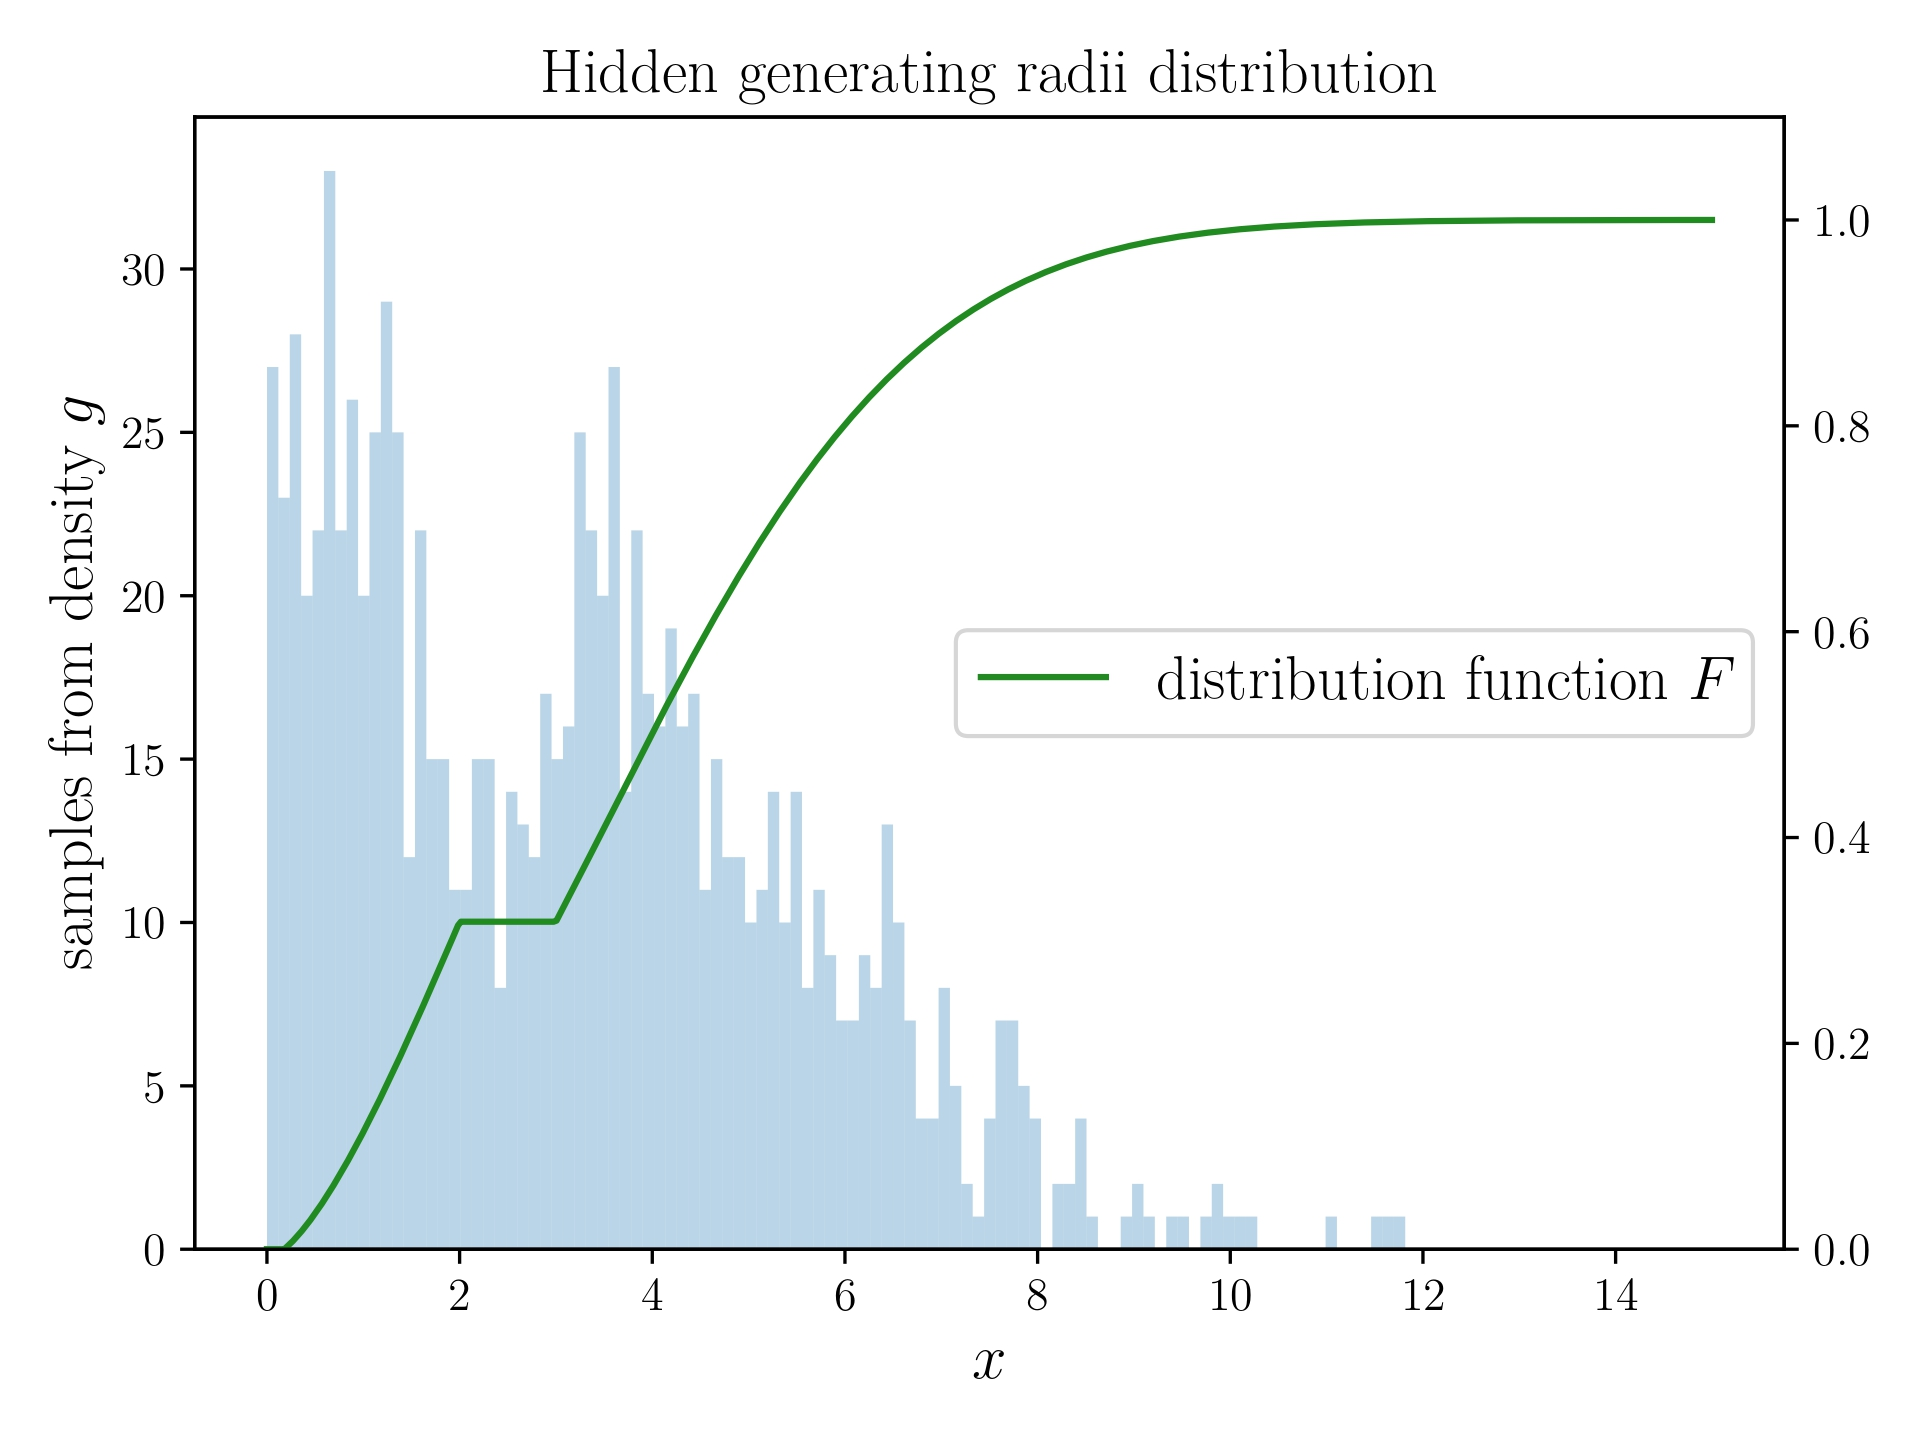
\includegraphics[width=6cm]{img/cdf_truth_page.jpg}
  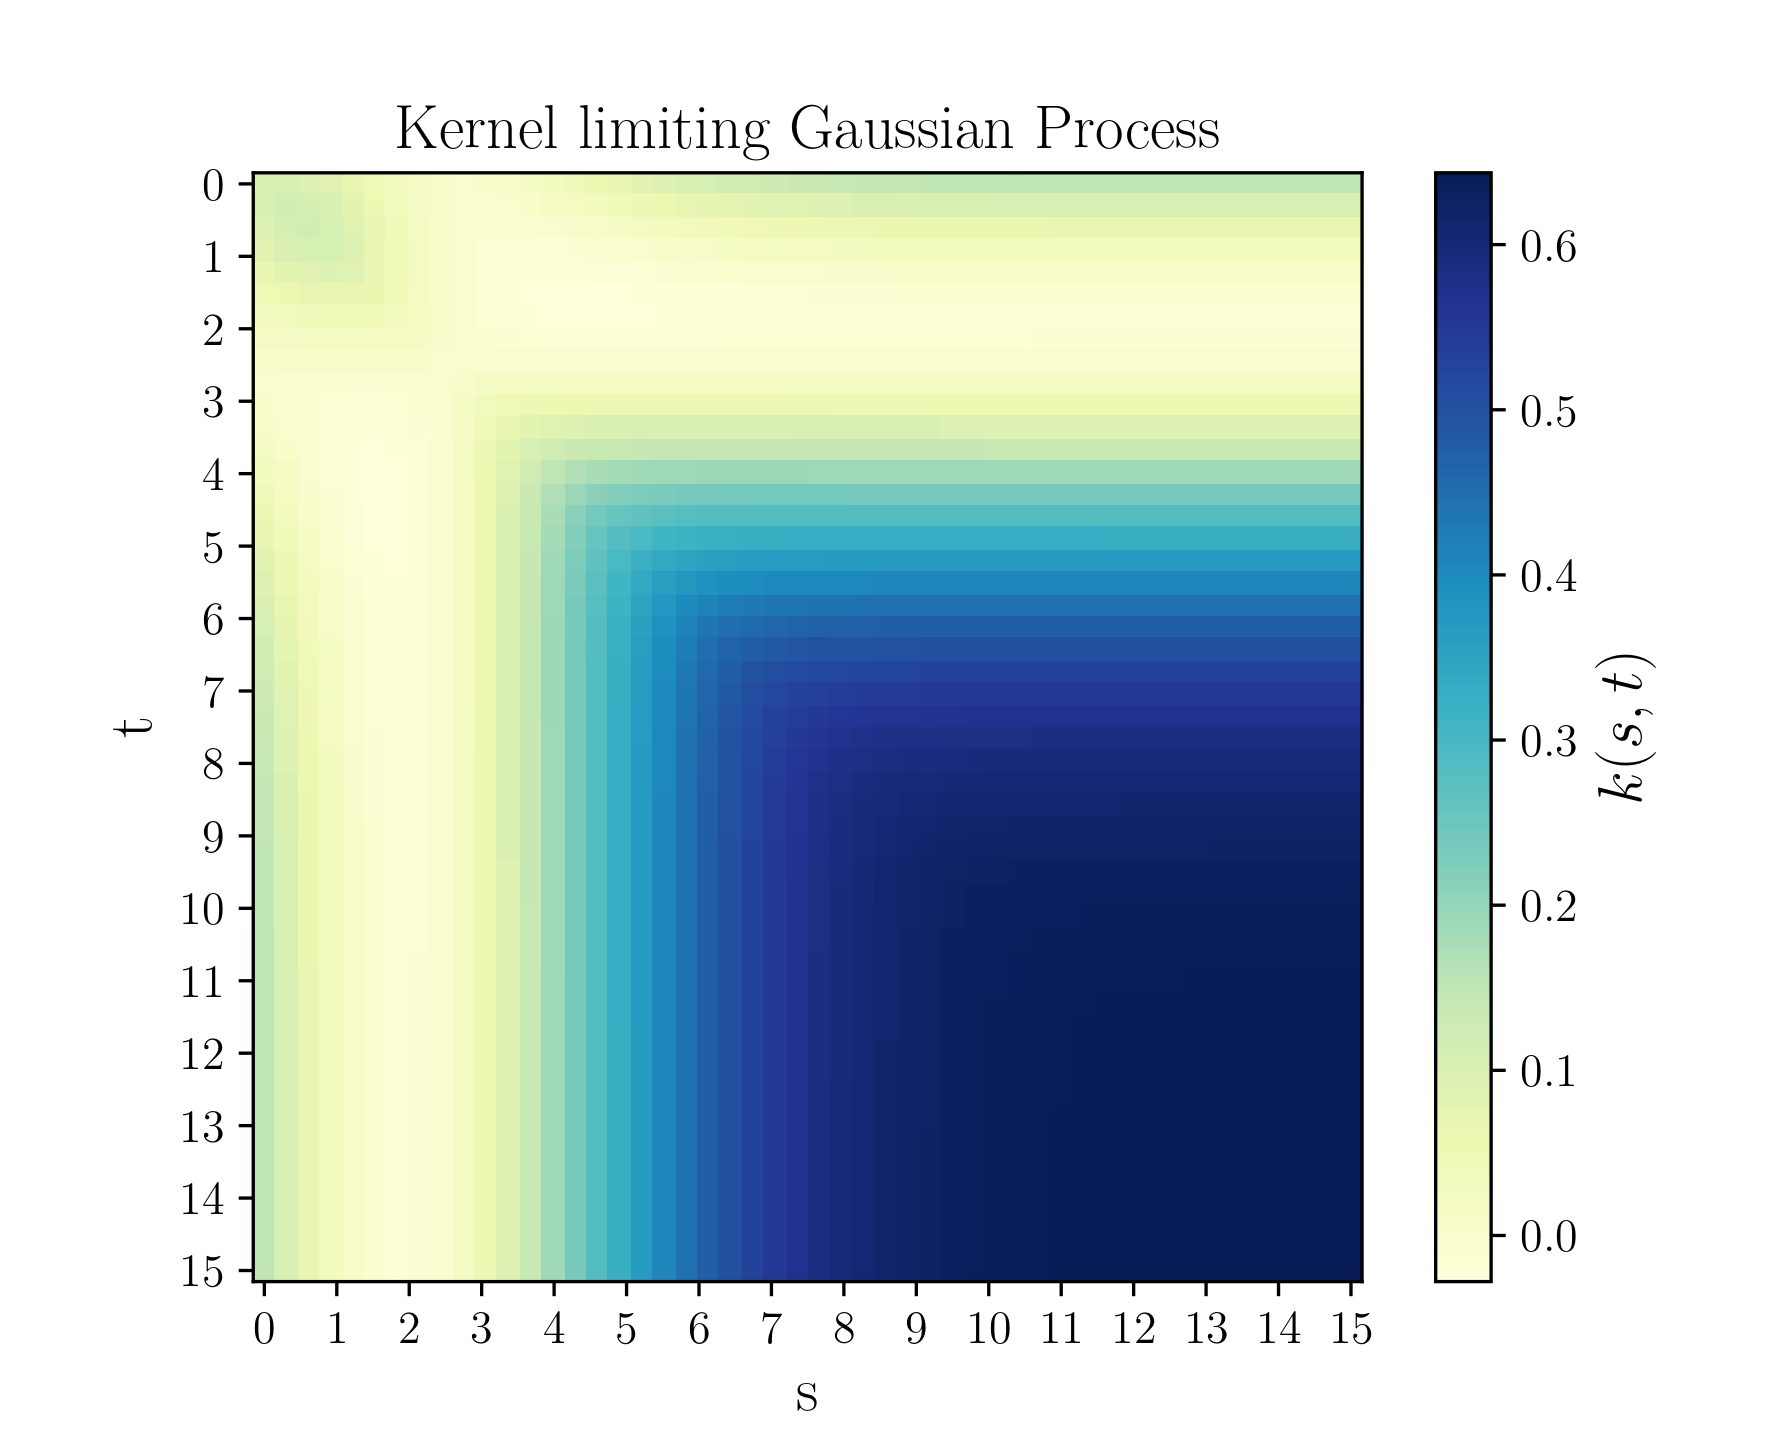
\includegraphics[width=5.75cm]{img/kernel_page.jpg}
  \setlength{\belowcaptionskip}{-4pt}
  \setlength{\abovecaptionskip}{0pt}
  \caption{Left panel: underlying cdf $F^*$ with samples from $g$. Right panel: representation of covariance structure of the limiting Gaussian Process $\mathbb{Z}_x$.}\label{fig: 1}
\end{figure}
\begin{figure}[ht]
  \centering
  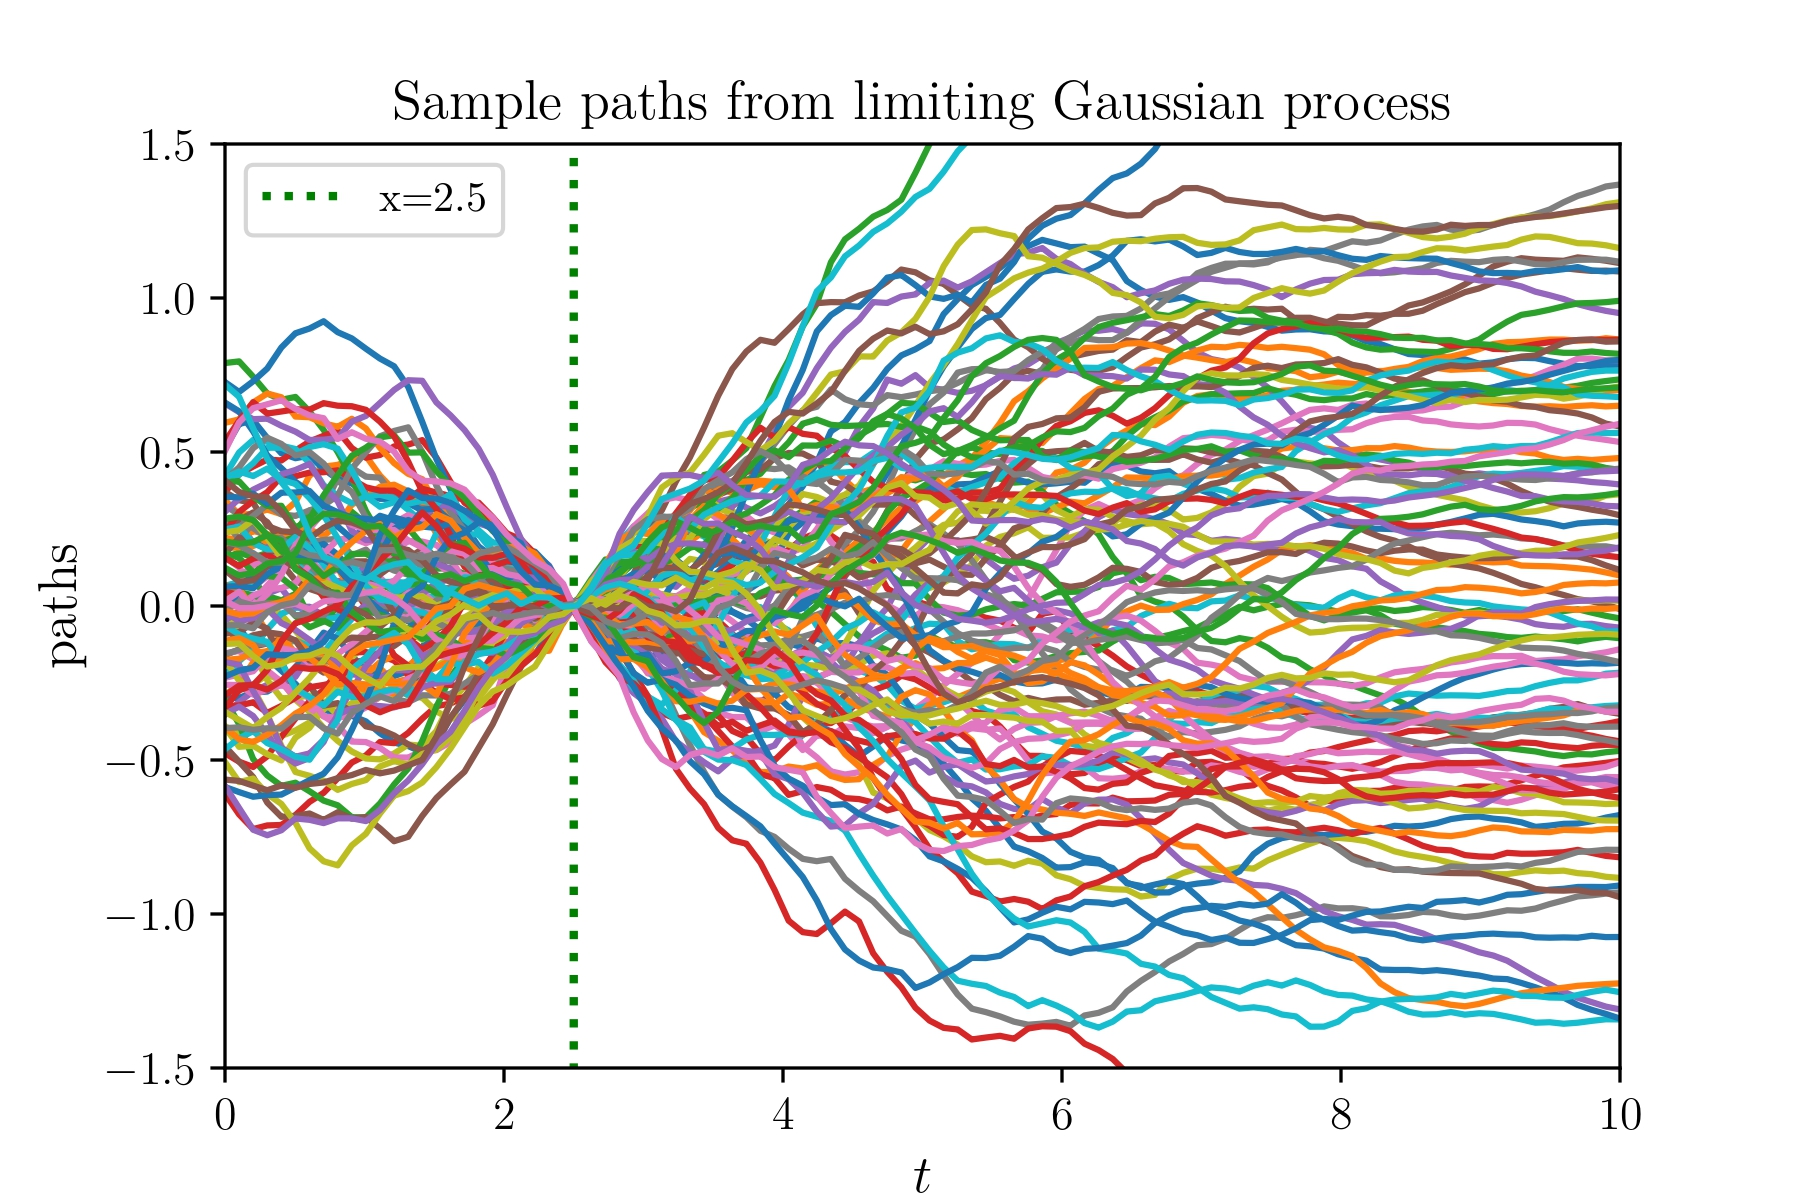
\includegraphics[width=6.2cm]{img/samplepahts_page.jpg}\hspace{-0.5cm}
  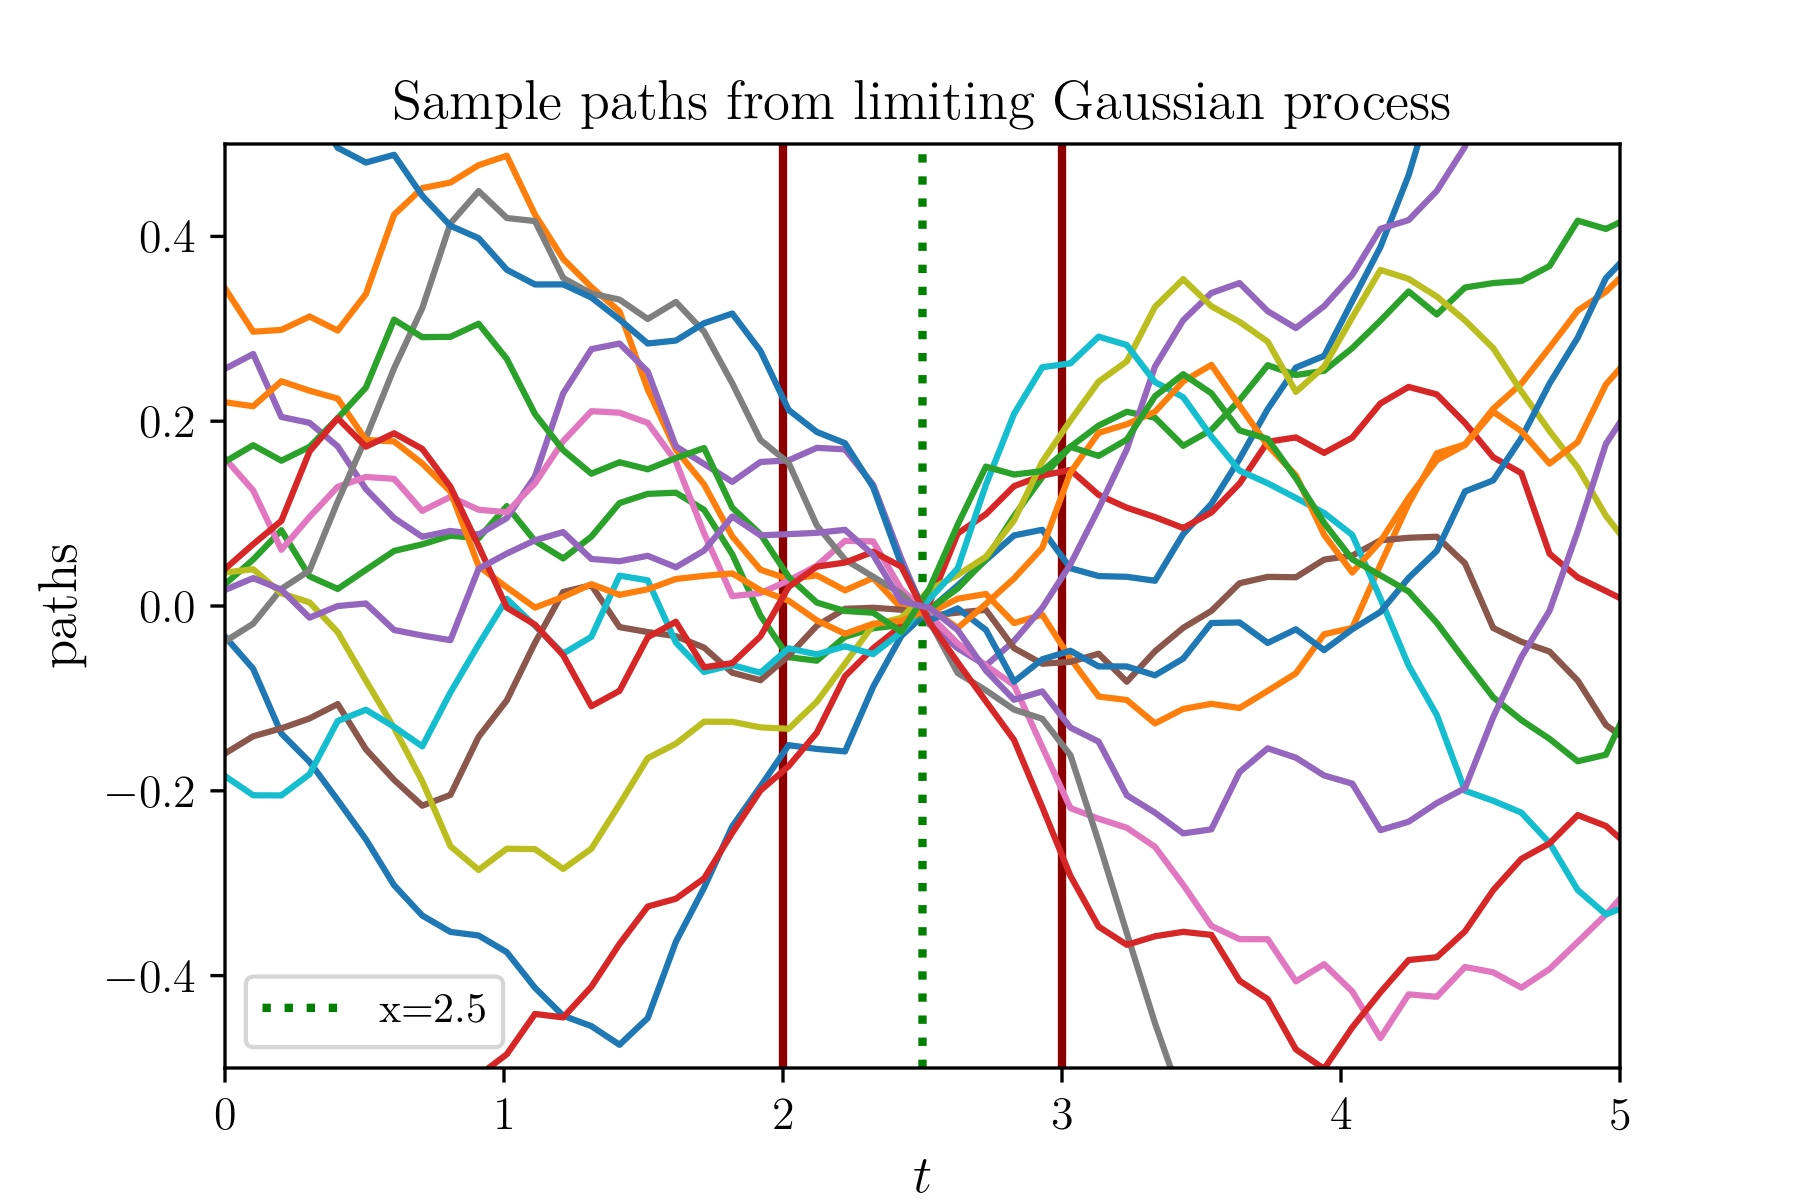
\includegraphics[width=6.2cm]{img/zoomsamplepahts_page.jpg}
  \setlength{\belowcaptionskip}{-4pt}
  \setlength{\abovecaptionskip}{-4pt}
  \caption{Left panel: $200$ samples from limiting Gaussian Process $\mathbb{Z}_x$. Right panel: zoom in on $15$ samples paths, putting into evidence the interval $[2,3]$.}\label{fig: 2}
\end{figure} 


In this setting, we show some simulations of the distribution of the limiting random variable of Theorem \ref{thm: distrib flat F at x}, above denoted by $L_x$. To do that, we compute the kernel given in \eqref{eq: covariance gauss process} of the limiting Gaussian process $\mathbb{Z}_x$. For the $F^*$ given in the left panel of Figure \ref{fig: 1}, the corresponding kernel is given in the right panel of Figure \ref{fig: 1}.
Subsequently, we simulate $200$ sample paths from the limiting Gaussian Process $\mathbb{Z}_x$ with the given kernel. These sample paths are shown in Figure \ref{fig: 2}. In the right panel of Figure \ref{fig: 2} we zoom in on the interval $[2,3]$ of interest and look at the behavior of $15$ selected sample paths. As we would expect, all sample paths pass through $(2.5,0)$.

In order to simulate the distribution of $L_x$, we use the fact that such random variable, by the proof of the theorem, is the right derivative of the least concave majorant of the Gaussian Process $\mathbb{Z}_x$ evaluated at $x = 2.5$.  With all the gathered samples from $L_x$ we looked at its estimated distribution and below we show some tests about the normality of the distribution of $L_x$. With the gathered samples, we see in Figure \ref{fig: 3} that we could not reject the null hypothesis that $L_x$ is normally distributed.

\begin{figure}
   \vspace{-0.1cm} 
  \centering
  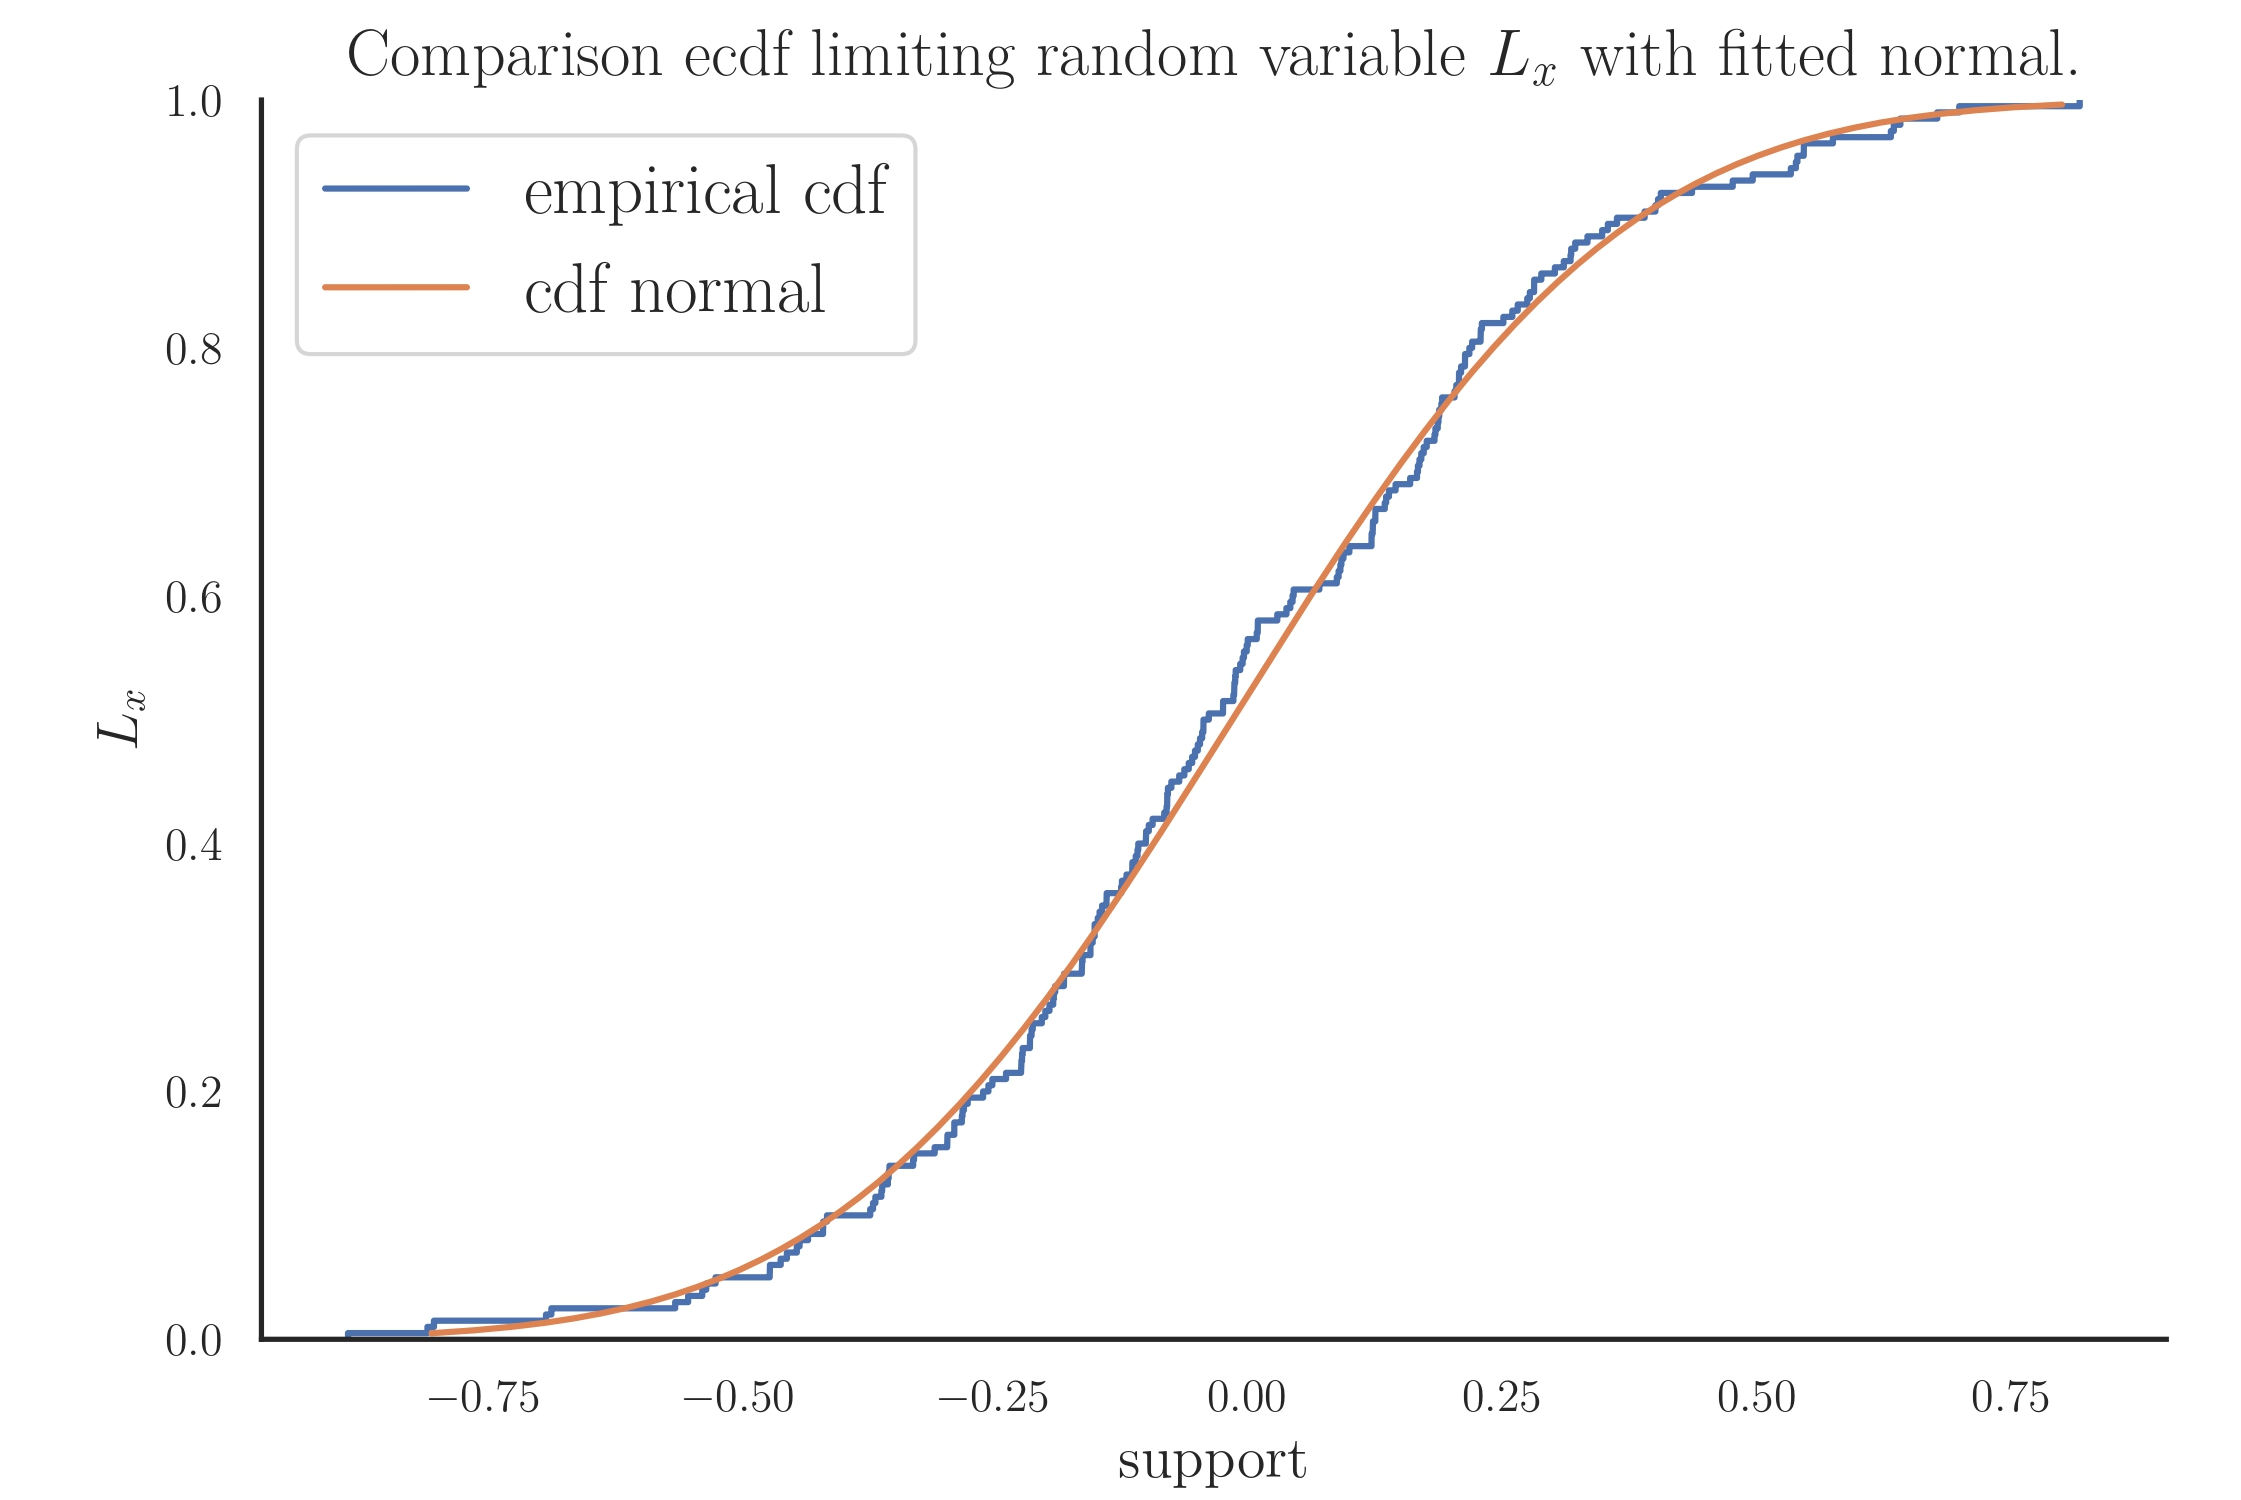
\includegraphics[width=6cm]{img/ecdfvsnormal_page.jpg}\hspace{-0.3cm}
  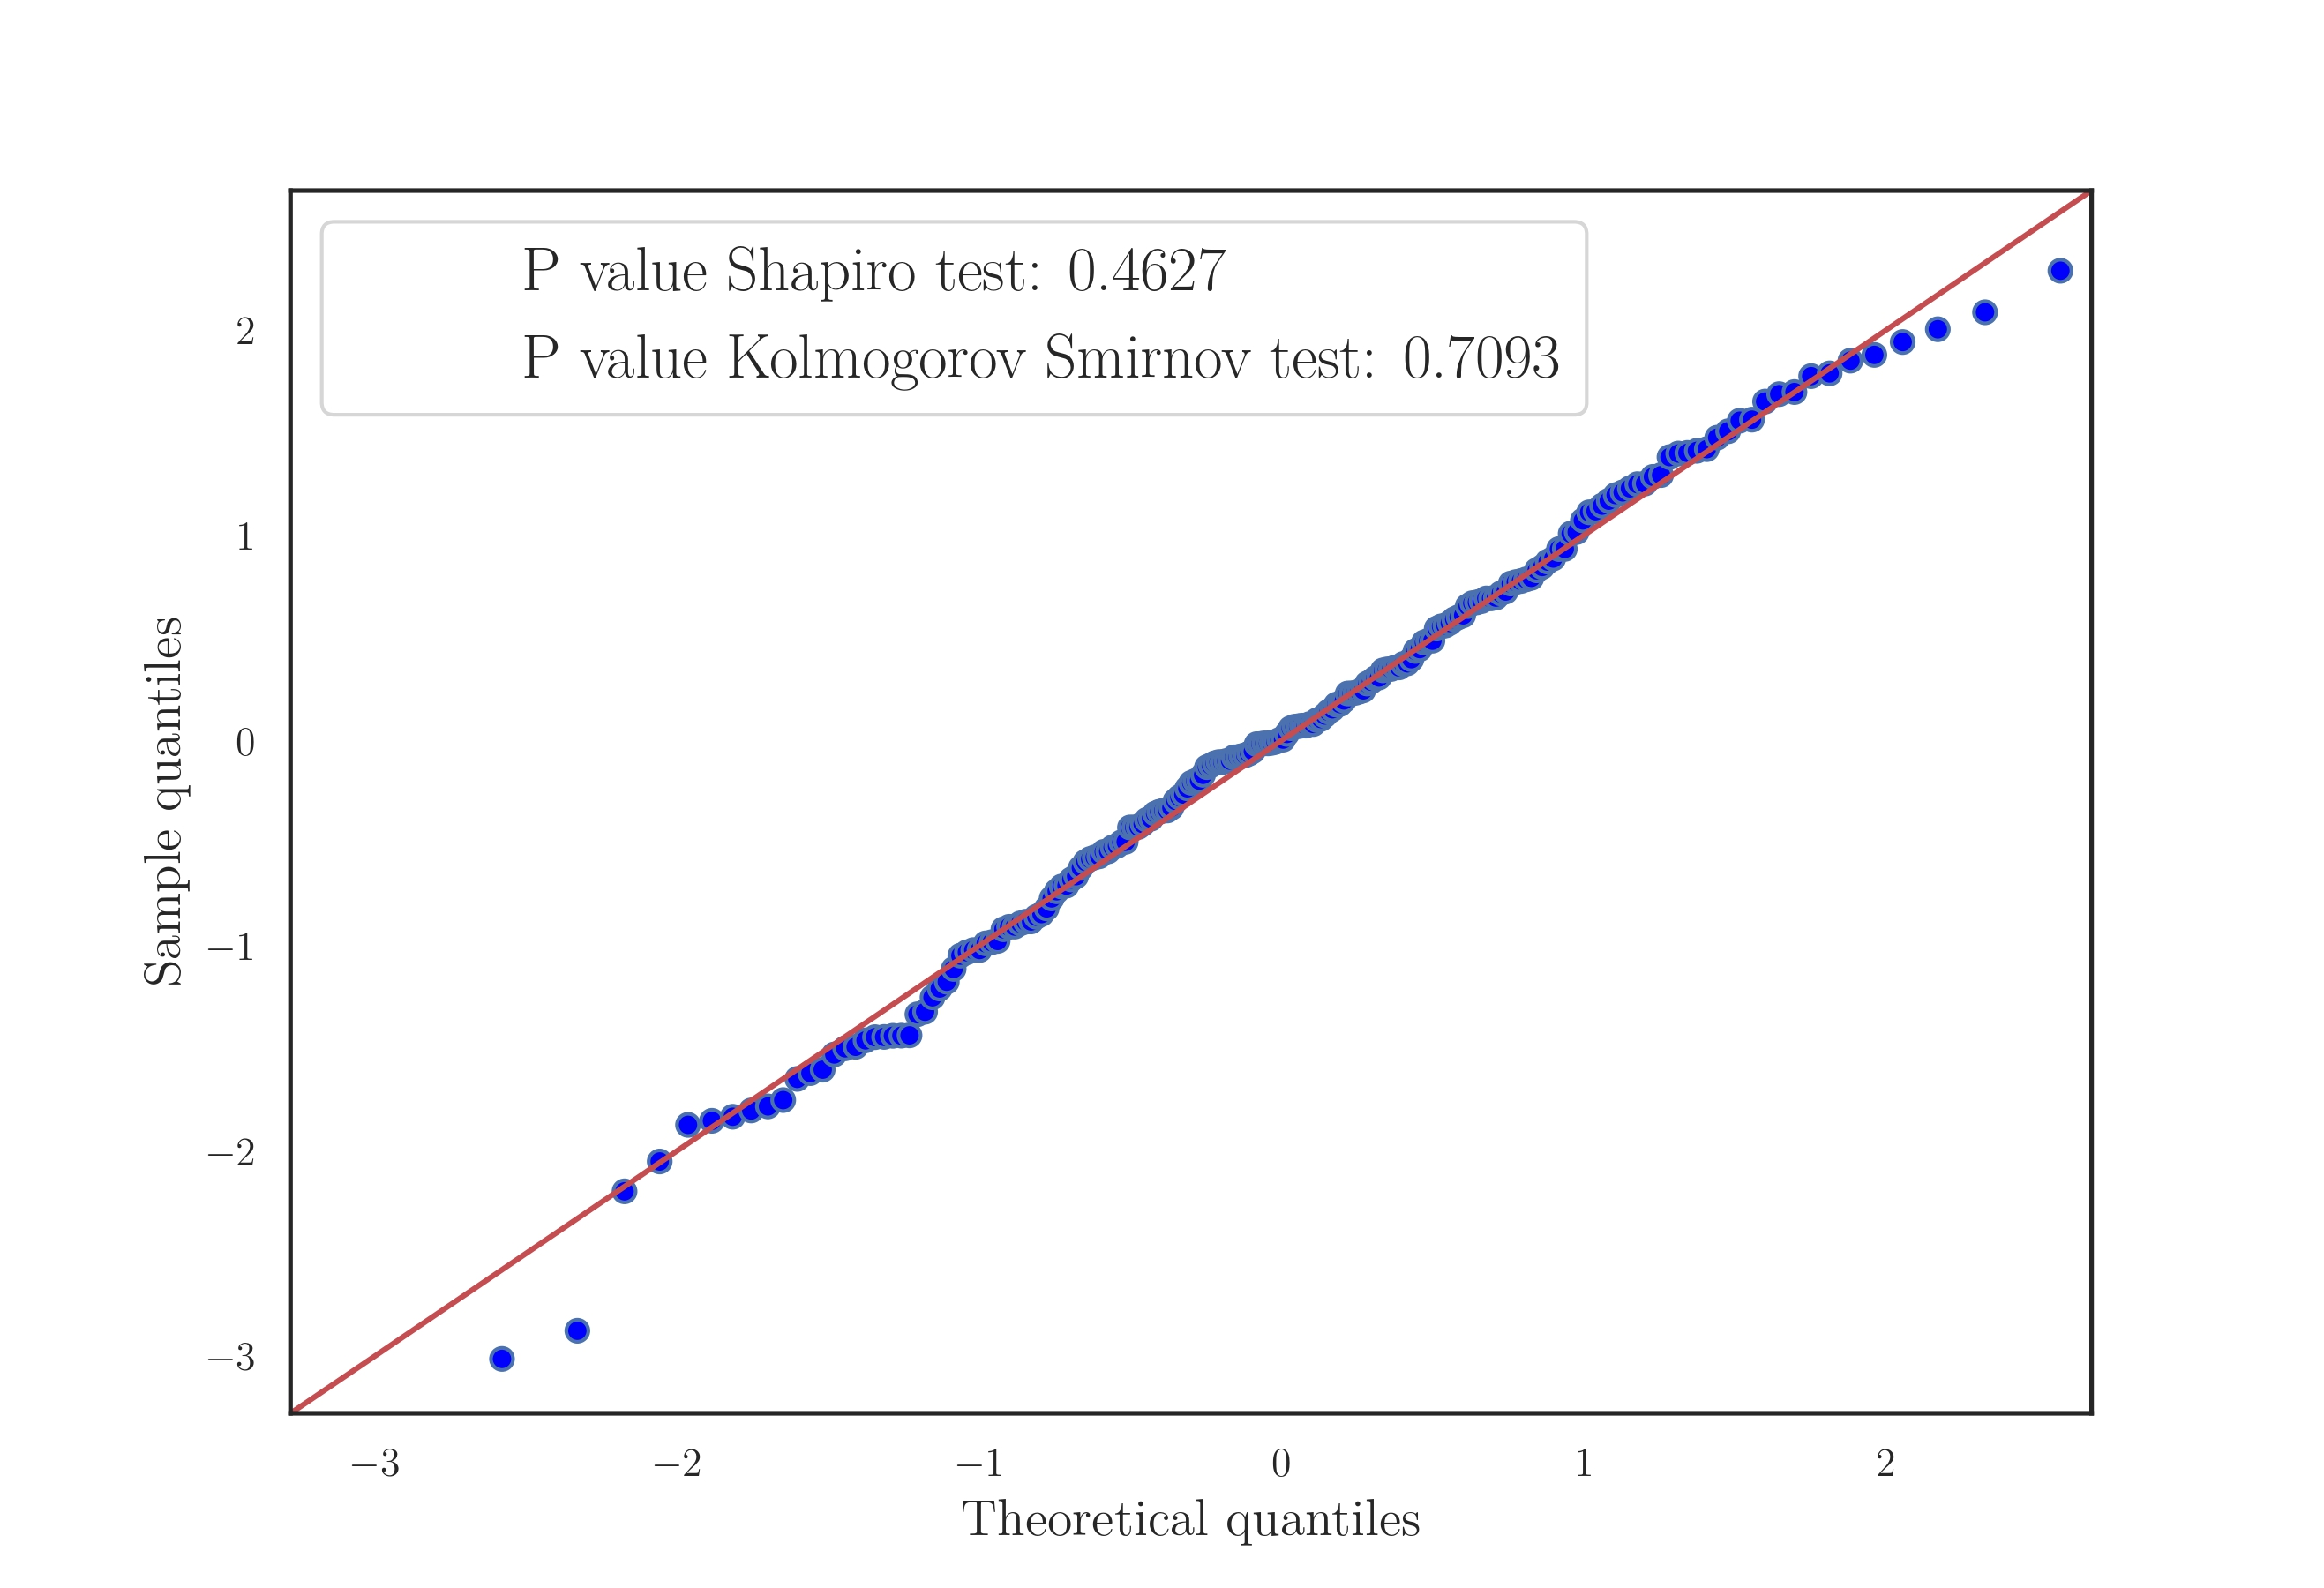
\includegraphics[width=6.5cm]{img/pvalues_page.jpg}
  \setlength{\belowcaptionskip}{-6pt}
  \setlength{\abovecaptionskip}{-4pt}
  \caption{Left panel: ecdf of limiting random variable $L_x$ compared to a suitably fitted normal. Right panel: qq-plot of $L_x$ compared to the fitted normal and p-values of the standard tests.}\label{fig: 3}
\end{figure}



\subsection{Local Asymptotic Minimax Theorem}

In this subsection, we show that the isotonic estimator (IIE) is asymptotically efficient, in the sense that its asymptotic variance is the smallest attainable. For this reason, we establish a statement about a lower bound of the minimax risk for any estimator sequence. We do this by constructing a parametric perturbation along the least favorable direction in the proximity of the true distribution function $F^*$. 

Let $x > 0$ be the point at which we want to estimate $F^*$. The existence of a least favorable path is a non-trivial matter. We will be guided by intuition in the construction of this path. We want to estimate is: $F^*(x) = 1 - V(x)/V(0)$. The local behavior at $x$ and $0$ of the kernels in the definitions of $V(x)$ and $V(0)$ is what essentially characterizes the estimation in Wicksell's problem and leads to the unusual rate $n^{-1/2}\sqrt{\log{n}}$. Thus, it should be enough to introduce a local perturbation of $F^*$ around $x$ and $0$. However, such perturbation must be tailored according to the local level of smoothness of the true $F^*$ near $x$ and $0$. Therefore, we need to identify such a level, and this is done in the following condition \eqref{eq: condition roughness infimum}.

The level of locality of the condition must be tied to the smoothness itself, because if the true $F^*$ is very rough around $x$ or $0$, then we expect a more stringent level of locality (and vice versa). Therefore we define the following intervals close to $p \in \{0,x\}$ for constants $\gamma_0 > \frac{1}{2}, \gamma_x > \frac{1}{2}$ to be determined later:
\begin{gather*}
\prescript{r}{}{\mathrm{K}}^{0}_n := \left[ n^{-\frac{1}{2\gamma_{\scaleto{0}{2.5pt}}}}, \eta_n  \right],\\
\prescript{l}{}{\mathrm{K}}^{x}_n := \left[ x - \eta_n, x - n^{-\frac{1}{2\gamma_{\scaleto{x}{2.5pt}}}} \right], \: \: \: \prescript{r}{}{\mathrm{K}}^{x}_n := \left[ x + n^{-\frac{1}{2\gamma_{\scaleto{x}{2.2pt}}}},x + \eta_n  \right],
\end{gather*}
where $\eta_n \downarrow 0$, $0 < \eta_n \leq 1, \: \forall \, n$ and $\exists \: \alpha \in (0,1)$ such that $\eta_n \gtrsim \frac{1}{\log^{\alpha}(n)}$. Now, let $\gamma_0, \gamma_x$ be the smallest constants greater than $1/2$, such that the true $F^*$, for $\mathrm{K}^p_n \in \{ \prescript{r}{}{\mathrm{K}}^{x}_n, \prescript{l}{}{\mathrm{K}}^{x}_n, \prescript{r}{}{\mathrm{K}}^{0}_n\}$ and therefore $p \in \{0,x\}$ satisfies:
\begin{align*}
    &\liminf_{n \rightarrow \infty } \inf_{\substack{x_1, x_2 \in \mathrm{K}^p_n }}\sqrt{n\log{n}}  \frac{|F^*(x_2)-F^*(x_1)|}{\Big|\log{\left\{\frac{p-x_1}{p-x_2} \right\}}\Big|} = \infty. \numberthis \label{eq: condition roughness infimum} 
\end{align*}

With condition \eqref{eq: condition roughness infimum}, our path can be shown to be well-defined and it is the least restrictive we can require. As we naturally would expect, the $\gamma_0, \gamma_x$ introduced above contain information about the local roughness of $F^*$ near $x$ and $0$. We illustrate this with our previous example \ref{example: cdf holder} and an additional example.
\begin{example}
Let us consider the same class of functions as in Example \ref{example: cdf holder}. These functions can be thought to be tightly Hölder smooth at $x$ and satisfy \eqref{eq: condition roughness infimum}. Let us consider the interval $\prescript{r}{}{\mathrm{K}}^{x}_n =\left[x+n^{-1 /(2 \gamma_x)}, x+\log (n)^{-\alpha}\right]$. If $F^*(u)=F^*(x)+K(u-x)^{\gamma_x}$ for $u \in \prescript{r}{}{\mathrm{K}}^{x}_n$, then
$$
\begin{aligned}
&\inf _{x_1, x_2 \in \prescript{r}{}{\mathrm{K}}^{x}_n}  \frac{\left|F^*\left(x_2\right)-F^*\left(x_1\right)\right|}{\left|\log \left\{\left(x-x_1\right) /\left(x-x_2\right)\right\}\right|} =K \inf_{ \substack{x_1, x_2 \in \prescript{r}{}{\mathrm{K}}^{x}_n \\ x_1<x_2}} \frac{\left(x_2-x\right)^{\gamma_x}-\left(x_1-x\right)^{\gamma_x}}{\log \left\{1+\left(x_2-x_1\right) /\left(x_1-x\right)\right\}}  \\
&=K \inf _{\substack{x_1, x_2 \in \prescript{r}{}{\mathrm{K}}^{x}_n \\ x_1<x_2}}\left(x_1-x\right)^{\gamma_x} \frac{\left[1+\left(x_2-x_1\right) /\left(x_1-x\right)\right]^{\gamma_x}-1}{\log \left[1+\left(x_2-x_1\right) /\left(x_1-x\right)\right]}  =K \gamma_x \inf _{x_1 \in \prescript{r}{}{\mathrm{K}}^{x}_n }\left(x_1-x\right)^{\gamma_x} \\
&=K \gamma_x n^{-1 / 2},
\end{aligned}
$$
because $\frac{(1+y)^\gamma-1}{\log (1+y)}$ is increasing in $y>0$ with limit $\gamma$ as $y \downarrow 0$.
\end{example}
\begin{example}
Condition \eqref{eq: condition roughness infimum}, which is similar to the conditions of \cite{10} (cf. (24) and (25)), is a consequence of a stronger on, namely: 
$$\liminf_{n \rightarrow \infty } \inf \frac{|F^*(x_2)-F^*(x_1)|}{|x_2 - x_1|^{\gamma_{\scaleto{x}{2.2pt}}} } > 0,$$ 
where the infimum is as in \eqref{eq: condition roughness infimum}. We show that it implies \eqref{eq: condition roughness infimum} on $\prescript{r}{}{\mathrm{K}}^{x}_n$:
\begin{align*}
    \inf_{\substack{x_1, x_2 \in \prescript{r}{}{\mathrm{K}}^{x}_n}} &\frac{F^*(x_2) - F^*(x_1)}{\log{\{\frac{x-x_1}{x-x_2} \}}} = \inf_{\substack{x_1, x_2 \in \prescript{r}{}{\mathrm{K}}^{x}_n }} \frac{|F^*(x_2)-F^*(x_1)|}{|x_2 - x_1|^{\gamma_{\scaleto{x}{2.2pt}}} } \frac{|x_2 - x_1|^{\gamma_{\scaleto{x}{2.2pt}}}}{\log{\left( 1 - \frac{x_2 - x_1}{x_2-x} \right)}}
\end{align*}
where, $x_1 < x_2$, both $x_1, x_2 \in \prescript{r}{}{\mathrm{K}}^{x}_n$ and thus $0<\frac{x_2 - x_1}{x_2 - x} <1$ going to zero as $n \rightarrow \infty$. The above expression, for all $n$ big enough behaves like in the previous example. Multiplied by $\sqrt{n\log{n}}$ \eqref{eq: condition roughness infimum} diverges to $\infty$.
\end{example}

The second fundamental assumption to obtain our minimax lower bound is that $g$ is continuous in a neighborhood of $x$ and in a right neighborhood of $0$. We will assume this all along. A sufficient condition to obtain this is that $F^*$ is locally Hölder continuous around $x$ and $0$ of degrees greater than $\frac{1}{2}$ (see Lemma \ref{lemma: bounded density} in Appendix \ref{sec: appendix chapter2}). We also note that from \eqref{eq: condition roughness infimum} we have $F^*(x)<1$.

We will now proceed with the construction of the path on the space of distribution functions and verify that it is well defined. The construction of our path is based on ideas from \cite{10}. Condition \eqref{eq: condition roughness infimum} gives us the appropriate $\gamma_0, \gamma_x$ that we use for the definition of the perturbation.
 For $u \geq 0$ define: 
\begin{align}\label{eq: path}
    F^*_{h_n}(u) = \frac{1}{D_{h_n}} \left( F^*(u) + h_{1,n} \int_{0}^{u} \chi_{{\scaleto{1,n}{4.5pt}}}(v) \, dv + h_{2,n} \int_{0}^{u} \chi_{{\scaleto{2,n}{4.5pt}}}(v-x) \, dv \right),
\end{align}
where for $\gamma_0 > \frac{1}{2}, \: \gamma_x > \frac{1}{2}$, using that $\int_{0}^{\infty} \chi_{{\scaleto{2,n}{4.5pt}}}(v-x) \, dv = 0$:
\begin{align*}
    &\chi_{{\scaleto{1,n}{4.5pt}}}(v)= (v)^{-1} \ind_{\left\{ n^{-1/(2\gamma_{\scaleto{0}{2.2pt}})} \leq v \leq \eta_n \right\}},  \\
    &\chi_{{\scaleto{2,n}{4.5pt}}}(v-x)= (v-x)^{-1} \ind_{\left\{ n^{-1/(2\gamma_{\scaleto{x}{2.2pt}})} \leq|v-x| \leq \eta_n \right\}}, \\
    &D_{h_n} = 1 + h_{1,n} \int_{0}^{\infty} \chi_{{\scaleto{1,n}{4.5pt}}}(v) \, dv + h_{2,n} \int_{0}^{\infty} \chi_{{\scaleto{2,n}{4.5pt}}}(v-x) \, dv \\
    &\quad \quad = 1 + h_{1,n} \int_{0}^{\infty} \chi_{{\scaleto{1,n}{4.5pt}}}(v) \, dv. 
\end{align*}
We will see that the truncation levels of the function $1/(v-x)$ proposed here above work, but they may not be unique. The function $\chi_{{\scaleto{i,n}{4.5pt}}}$, with similar truncation levels, was introduced for the first time in \cite{10}, however there it was not used directly for the perturbation as done here and the assumption $\gamma_0 = \gamma_x$ was used.

We will check that the perturbation $ F^*_{h_n}$ is well defined for: 
\begin{align}\label{eq: h_i}
    h_{i,n}= \frac{h_i}{\sqrt{n \log{n}}}, \quad h_i \in \mathbb{R}, \quad i=1,2. 
\end{align}

\begin{figure}
    \vspace{-0.1cm}
  \centering
  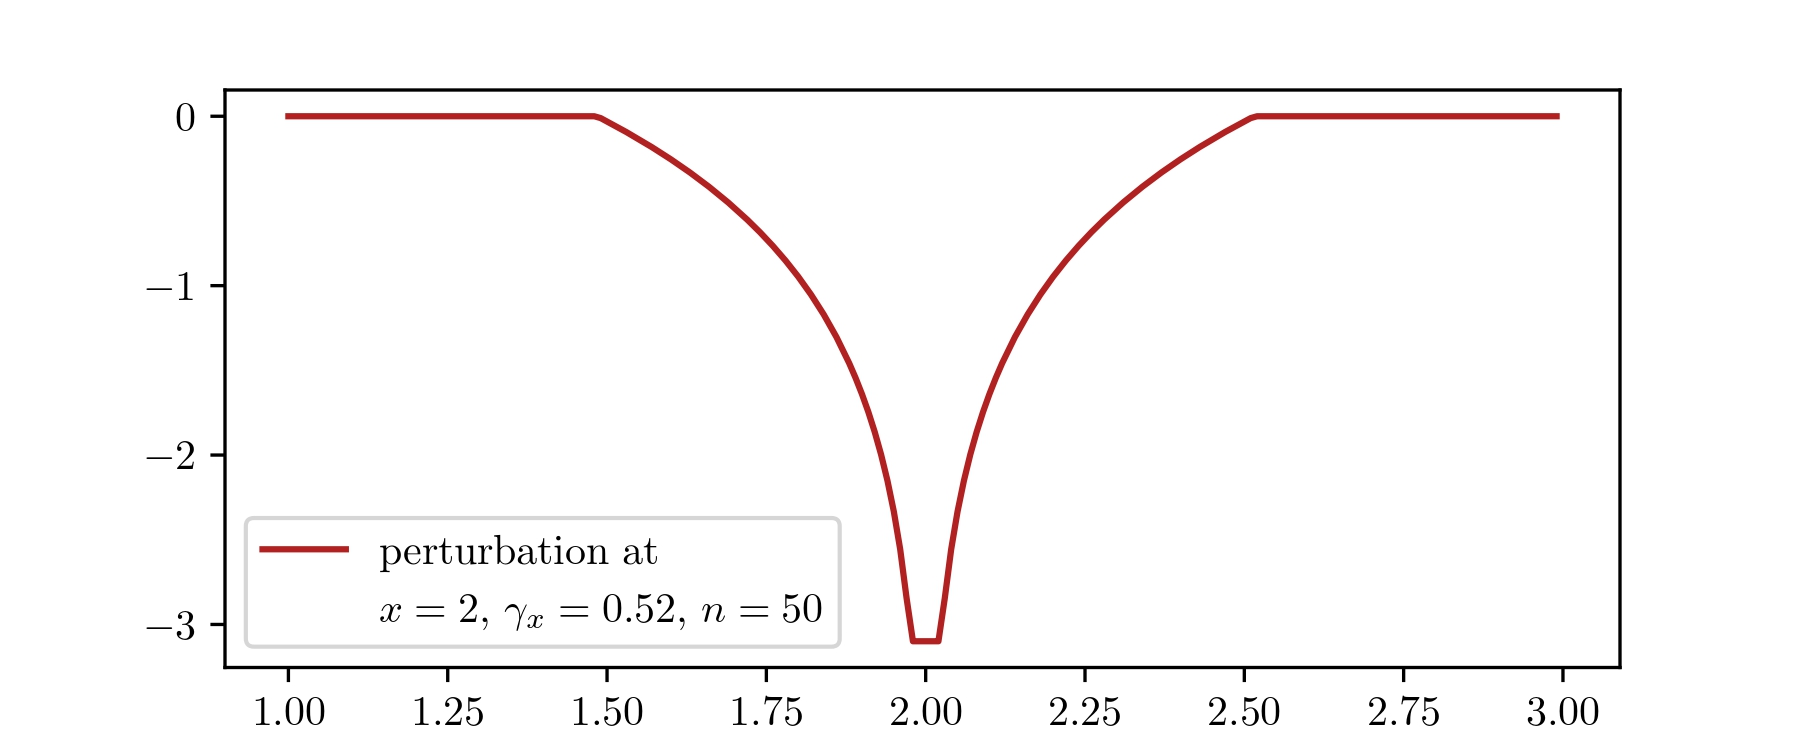
\includegraphics[width = 8cm]{img/perturbation_page.jpg}
  \setlength{\belowcaptionskip}{-4pt}
  \caption{Visualization of $\int_{0}^{u} \chi_{{\scaleto{2,n}{4.5pt}}}(v-x)dv$ for $x=2$, $n=50$ and $\gamma_x = 0.52$, $\eta_n = 1/\sqrt{\log{n}}$.} \label{fig: perturbation}
\end{figure}

First, we compute the case of $\chi_{{\scaleto{2,n}{4.5pt}}}$, to show how the perturbation looks like:
\begin{align*}
    &\int_{0}^{u} \chi_{{\scaleto{2,n}{4.5pt}}} (v-x) \, dv = \log{\left(\eta^{-1}_n (x-u) \right)}\ind_{\big\{ x - \eta_n \leq u \leq x - n^{-\frac{1}{2 \gamma_{\scaleto{x}{2.2pt}}}} \big\}} +\\
    &\quad + \log{\left( \eta^{-1}_n \, n^{-\frac{1}{2 \gamma_{\scaleto{x}{2.2pt}}}} \right)} \bigg( \ind_{\big\{ u > x - n^{-\frac{1}{2 \gamma_{\scaleto{x}{2.2pt}}}} \big\}} - \ind_{\big\{ u > x + \eta_n \big\}} \bigg)+\\
    &\quad + \log{\left(\eta^{-1}_n(u-x) \right)} \ind_{\big\{x + n^{-\frac{1}{2 \gamma_{\scaleto{x}{2.2pt}}}} \leq u \leq x+\eta_n  \big\}}. \numberthis \label{eq: written out perturbation}
\end{align*}
Figure \ref{fig: perturbation} visualizes the perturbation $\int_{0}^{u} \chi_{{\scaleto{2,n}{4.5pt}}}(v-x)dv$ in \eqref{eq: written out perturbation}. It is immediate from \eqref{eq: written out perturbation} that this perturbation is continuous and therefore the summation with $F^*$ results in a function $F^*_{h_n}$ that is right-continuous. Moreover, thanks to the normalization $D_{h_n}$, $\lim_{u \rightarrow + \infty} F^*_{h_n} (u) =1$ and, from the definition of $F^*_{h_n}$, note that $\lim_{u \rightarrow 0} F^*_{h_n} (u) =0$.
What is not evident is if $F^*_{h_n}$ is non-decreasing. Intuitively, for this to be true, we need $F^*$ to be "increasing enough" to compensate for the negative drop introduced by the perturbation. Condition \eqref{eq: condition roughness infimum} ensures that this is the case.  
\begin{lemma}\label{lemma: non decreasing F_h}
    For all $n$ sufficiently large, $F^*_{h_n}$ is non decreasing.
\end{lemma}
The \hyperlink{proof of lemma 5}{proof} of this lemma is provided in Appendix \ref{sec: appendix chapter2}.  We start by stating the most interesting result of this section which is the so-called LAM (locally asymptotically minimax) theorem and it entails the minimax risk for any estimator sequence. The proof of this theorem requires a few additional technical statements (the LAN expansion and the expression of the derivative of the functional of interest), which will be provided right after.
\begin{theorem}[LAM]\label{thm: LAM}
    Let $\gamma_0, \gamma_x$ be the smallest constants above $\frac{1}{2}$ such that $F^*$ satisfies \eqref{eq: condition roughness infimum}. Let $J=  \frac{\pi^2 }{8 m^2_0 } \operatorname{diag}\left(\frac{1}{\gamma_{\scaleto{0}{2.5pt}} g(0)}, \frac{1}{ \gamma_{\scaleto{x}{2.2pt}} g(x)}\right)$, $\dot{\psi} = \begin{bmatrix} \frac{1}{2\gamma_{\scaleto{0}{2.5pt}}} (1-F^*(x)) & - \frac{1}{2\gamma_{\scaleto{x}{2.2pt}}} \end{bmatrix}^{\top}$, $g$ as in \eqref{eq: density of the observations}, and $\ell$ be a bowl-shaped loss function, i.e., $\ell$ is non-negative, symmetric and subconvex. Then for every estimator sequence $\left( F^*_n(x)\right)_{n \in \mathbb{N}}$:
    \begin{align}\label{eq: LAM}
    \sup_{\substack{I \subset \mathbb{R}^2 \\ I \: \textup{finite}}} \liminf_{n \rightarrow \infty} \sup _{h \in I} \ex_{h} \ell\left(\sqrt{\frac{n}{\log{n}}}\left(F^*_n(x)- F^*_{h_n}(x)\right)\right) \geq \ex \ell(L) .
    \end{align}
The first supremum is taken over all finite subsets $I$ of $\mathbb{R}^2$, the expectation $\ex_h$ is under $G_{F^*_{h_n}}$, the probability measures associated to the perturbed densities $g_n$ in \eqref{eq: g_n}, and $L \sim N (0, \dot{\psi}^{\top} J^{-1} \dot{\psi})$;
\begin{align*}
    {\dot{\psi}}^{\top} J^{-1} \dot{\psi} = \frac{4m^2_0}{\pi^2} \left(\frac{g(x)}{2\gamma_x} + (1-F^*(x))^2 \frac{g(0)}{2\gamma_0} \right).
\end{align*}
\end{theorem}
\begin{proof}
The proof is an immediate application of Theorem 3.11.5 from \cite{5}, using Theorem \ref{thm: LAN} and Lemma \ref{lemma: hadamard derivative} given below.
\end{proof}

Now we proceed by proving the technical results needed for the proof of Theorem \ref{thm: LAM}. First, we show that given the path \eqref{eq: path}, we can obtain a LAN expansion (see \cite{6}, Chapter 7).
In the statement of the LAN Theorem, the perturbed density of the observations $Z_i$ appears. Therefore, using \eqref{eq: path}, we derive it before proceeding:
\begin{align*}
    g_n (z) &= \frac{1}{2m_{h_n}} \int_{z}^{\infty} \frac{dF^*_{h_n} (v)}{\sqrt{v-z}}  \numberthis \label{eq: g_n} \\
    &= \frac{1}{2m_{h_n} D_{h_n}} \left\{ \int_{z}^{\infty} \frac{dF^*(v)}{\sqrt{v-z}} + h_{1,n} \int_{z}^{\infty} \frac{\chi_{{\scaleto{1,n}{4.5pt}}}(v)}{\sqrt{v-z}} \, dv + h_{2,n} \int_{z}^{\infty} \frac{\chi_{{\scaleto{2,n}{4.5pt}}}(v-x)}{\sqrt{v-z}} \, dv \right\}.
\end{align*}
where $m_{h_n} = \int_{0}^{\infty} \sqrt{s} \, dF^*_{h_n} (s)$, analogously to $m_0$.

\begin{theorem}[LAN expansion]\label{thm: LAN}
Let $\gamma_0, \gamma_x$ be constants above $\frac{1}{2}$ such that $F^*$ satisfies \eqref{eq: condition roughness infimum}. Let $g$ be continuous in a neighborhood of $x$ and in a right-neighborhood of $0$. Then for $h^{\top} = [h_1,h_2] \in \mathbb{R}^2$, $h_n = \frac{h}{\sqrt{n\log{n}}}$, $F^*_{h_n}$ as in \eqref{eq: path} and accordingly $g_n$ in \eqref{eq: g_n}:
\begin{align*}
    \sum_{i=1}^{n} \log{\frac{g_n (Z_i)}{g(Z_i)}} = h^{\top} \Delta_n - \frac{1}{2} h^{\top} J h + o_p (1),
\end{align*}
where the $o_p(1)$ is under $Z_1,\cdots,Z_n \stackrel{\scaleto{i.i.d.}{3.2pt}}{\sim} g$, for $J =  \frac{\pi^2 }{8 m^2_0 } \operatorname{diag}\left(\frac{1}{\gamma_{\scaleto{0}{2.5pt}} g(0)}, \frac{1}{ \gamma_{\scaleto{x}{2.2pt}} g(x)}\right)$ and $\Delta_n \rightsquigarrow N\left( 0, J \right)$, where:
\begin{align*}
    \Delta_n = \begin{bmatrix} \sum_{i=1}^n \frac{1}{ m_{h_n} D_{h_n} \sqrt{n\log{n}} } \left( \frac{1}{2g(Z_i)} \int_{Z_i}^{\infty} \frac{\chi_{{\scaleto{1,n}{3.5pt}}}(v)}{\sqrt{v-Z_i}} \, dv - \int_{0}^{\infty} \sqrt{v} \chi_{{\scaleto{1,n}{4.5pt}}}(v) \, dv \right)\\ \sum_{i=1}^n \frac{1}{ m_{h_n} D_{h_n} \sqrt{n\log{n}}} \left( \frac{1}{2g(Z_i)} \int_{Z_i}^{\infty} \frac{\chi_{{\scaleto{2,n}{3.5pt}}} (v-x)}{\sqrt{v-Z_i}} \, dv - \int_{0}^{\infty} \sqrt{v} \chi_{{\scaleto{2,n}{4.5pt}}}(v - x) \, dv \right) \end{bmatrix}.
\end{align*}
\end{theorem}
\begin{proof}

The structure of the proof of this result is as follows. First, we give the expansions of the functions $\int_z^{\infty} \frac{\chi_{{\scaleto{2,n}{3.5pt}}}(v-x) }{\sqrt{v-z}} \, d v, \: \int_{z}^{\infty} \frac{\chi_{{\scaleto{1,n}{3.5pt}}}(v)}{\sqrt{v-z}} \, dv$ that will highlight the leading terms that contribute to the limiting behavior. 

Next, we use the obtained approximations to write out the Taylor approximation of the logarithm and prove some additional relations that will eventually give the LAN. Finally, we show that the remaining terms are negligible. First of all, using the definition of $F^*_{h_n}$ in \eqref{eq: path}, we obtain:
\begin{align*}
    \frac{g_{n} (z)}{g (z)} = \frac{1}{m_{h_n} D_{h_n}} \left\{ m_0+ \frac{h_{1,n}}{2g(z)} \int_{z}^{\infty} \frac{\chi_{{\scaleto{1,n}{4.5pt}}}(v)}{\sqrt{v-z}} \, dv + \frac{h_{2,n}}{2g(z)} \int_{z}^{\infty} \frac{\chi_{{\scaleto{2,n}{4.5pt}}} (v-x)}{\sqrt{v-z}} \, dv \right\}.
\end{align*}
Then using \eqref{eq: approximation xi} (see Lemma \ref{lemma: expansion GL} proved in Appendix \ref{sec: appendix chapter2}): 
\begin{align*}
& \int_z^{\infty} \frac{\chi_{{\scaleto{2,n}{4.5pt}}}(v-x) }{\sqrt{v-z}} \, d v = \left\{ \frac{\pi}{\sqrt{z-x}} + O\left(\eta_n^{-\frac{1}{2}}\right)  \right\} \ind_{\left\{ n^{-\frac{1}{2 \gamma_{\scaleto{x}{2.2pt}}}} \leq z-x \leq \eta_n \right\}} + \numberthis \label{eq: only term that matters in expansion}\\
& +O\left(n^{\frac{1}{4\gamma_{\scaleto{x}{2.2pt}}}}\right) \ind_{\left\{ -n^{-\frac{1}{2 \gamma_{\scaleto{x}{2.2pt}}}}  \leq z-x \leq n^{-\frac{1}{2 \gamma_{\scaleto{x}{2.2pt}}}} \right\}} +  O\left(\eta_n^{-\frac{1}{2}}\right) \ind_{\left\{ z-x \leq - \eta_n \right\}} + \\
& + \left\{ O\left(n^{-\frac{1}{2\gamma_{\scaleto{x}{2.2pt}}}}(x-z)^{-\frac{3}{2} }\right)+O\left(\eta_n^{-\frac{1}{2}}\right) \right\} \ind_{\left\{ - \eta_n \leq z-x \leq - n^{-\frac{1}{2 \gamma_{\scaleto{x}{2.2pt}}}}\right\}}. \numberthis \label{eq: expansion zeta}
\end{align*}
The proof of Lemma \ref{lemma: expansion GL} has the following relation as an important ingredient:
\begin{align}\label{eq: abel integral pi}
 \int_u^{\infty} \frac{1}{t \sqrt{t-u}} \, d t=\pi \ind_{\{u \geq 0\}} u^{-1 / 2}, 
\end{align}
which follows from: $\int_{1}^{\infty} \frac{1}{t \sqrt{t-1}} dt = \pi$.
We will see that asymptotically the only term that matters is the first one in \eqref{eq: only term that matters in expansion}. It is immediate to see that $\sup_u | \int_{0}^{u} \chi_{{\scaleto{2,n}{4.5pt}}}(v-x)dv | = O( \log{\left( \eta_n^{-1} n^{1/2\gamma_x} \right)})$, once multiplied by $h_2/\sqrt{n\log{n}}$ goes to zero as $n \rightarrow \infty$. Note also that using the same computations as in equation \eqref{eq: written out perturbation} also for $\chi_{{\scaleto{1,n}{4.5pt}}}$, it follows that $D_{h_n} =1+o(1)$. 

Denote by: $A^{i,x}_n := \left\{n^{-\frac{1}{2\gamma_{\scaleto{x}{2.2pt}}}} \leq Z_i^x \leq \eta_n \right\} $, where $Z_i^x := Z_i - x$. As will be seen, the only contributing term is $\pi \ind_{A^{i,x}_n} / \sqrt{Z_i-x}$, we denote all the remainder terms by $R_{i}^{n,x}$ and it is immediate to see that:
\begin{align*}
& R_{i}^{n,x} = O\left(\eta_n^{-\frac{1}{2}}\right) \Big\{ \ind_{\big\{ - \eta_n \leq Z_i^x \leq - n^{-\frac{1}{2\gamma_{\scaleto{x}{2.2pt}}}} \big\}} + \ind_{\left\{ Z_i^x \leq - \eta_n  \right\}} + \ind_{A^{i,x}_n} \Big\} + \\
& O\left(n^{-\frac{1}{2\gamma_{\scaleto{x}{2.2pt}}}}(x-Z_i)^{-\frac{3}{ 2}}\right) \ind_{\big\{ - \eta_n \leq Z_i^x \leq - n^{-\frac{1}{2\gamma_{\scaleto{x}{2.2pt}}}} \big\}}  +O\left(n^{\frac{1}{4\gamma_{\scaleto{x}{2.2pt}}}}\right)\ind_{\big\{ -n^{-\frac{1}{2\gamma_{\scaleto{x}{2.2pt}}}}  \leq Z_i^x \leq n^{-\frac{1}{2\gamma_{\scaleto{x}{2.2pt}}}} \big\}}
\end{align*}
Analogously, we define $R^{n,0}_i$. Using the Taylor expansion of the logarithm with Peano residual, and \eqref{eq: expansion zeta}:
\begin{align*}
    &\sum_{i=1}^{n} \log{\frac{g_n (Z_i)}{g(Z_i)}} = \sum_{i=1}^{n} \Bigg\{ \frac{1}{m_{h_n} D_{h_n}} \bigg[ m_0 - m_{h_n} D_{h_n} + \frac{h_{1,n}}{2g(Z_i)} \int_{Z_i}^{\infty} \frac{\chi_{{\scaleto{1,n}{4.5pt}}}(v)}{\sqrt{v-Z_i}} \, dv + \\ 
    &+ \frac{h_{2,n}}{2g(Z_i)} \int_{Z_i}^{\infty} \frac{\chi_{{\scaleto{2,n}{4.5pt}}}(v-x)}{\sqrt{v-Z_i}} \, dv \bigg] - \frac{1}{2} \bigg[ \frac{m_0 - m_{h_n} D_{h_n}}{m_{h_n} D_{h_n}} + \frac{h_{1,n}}{2 m_{h_n} D_{h_n} g(Z_i)} \bigg(\frac{\pi \ind_{A^{i,0}_n}}{\sqrt{Z_i}}   \\
    & + R_n^{i,0} \bigg) + \frac{h_{2,n}}{2 m_{h_n} D_{h_n} g(Z_i)} \bigg(\frac{\pi \ind_{A^{i,x}_n}}{\sqrt{Z_i -x}}  + R_n^{i,x} \bigg) \bigg]^2 \hspace{-0.2cm} + o_p\Bigg( \bigg[ \frac{m_0 - m_{h_n} D_{h_n}}{m_{h_n} D_{h_n}} + \numberthis \label{eq: LAN exp} \\
    & \hspace{-0.05cm} + \frac{h_{1,n}}{2 m_{h_n} D_{h_n} g(Z_i)} \bigg(\frac{\pi \ind_{A^{i,0}_n}}{\sqrt{Z_i}}  + R_n^{i,0} \bigg) + \frac{h_{2,n}}{2 m_{h_n} D_{h_n} g(Z_i)} \bigg(\frac{\pi \ind_{A^{i,x}_n}}{\sqrt{Z_i -x}} + R_n^{i,x} \bigg) \bigg]^2 \Bigg) \Bigg\}.
\end{align*}
The Taylor expansion of the logarithm is granted by relation \eqref{eq: converge to zero for Taylor} (see Appendix \ref{sec: appendix chapter2} for its \hyperlink{proof of lemma 6}{proof}).
For $\zeta_{1,n} (z) := \int_{z}^{\infty} \frac{\chi_{{\scaleto{1,n}{3.5pt}}} (v)}{\sqrt{v-z}} \, dv, $ and for $\zeta_{2,n} (z - x) := \int_{z}^{\infty} \frac{\chi_{{\scaleto{2,n}{3.5pt}}} (v-x)}{\sqrt{v-z}} \, dv$ and $F^*$ as in \eqref{eq: condition roughness infimum}; then in probability: 
\begin{align}\label{eq: converge to zero for Taylor}
    \max_{1 \leq i \leq n} &\bigg|\frac{h_{1,n} \zeta_{1,n}(Z_i )}{ g(Z_i)} + \frac{h_{2,n}\zeta_{2,n} (Z_i - x)}{ g(Z_i)} \bigg| \rightarrow 0.
\end{align}
Now we provide a lemma on the normal behavior of the term inside the first square parenthesis in \eqref{eq: LAN exp}.
\begin{lemma}\label{lemma: lindeberg convergence}
For $F^*$ as in \eqref{eq: condition roughness infimum} and $h_{i,n}, \: i = 1,2$ as in \eqref{eq: h_i}:
\begin{align*}
    \frac{1}{m_{h_n} D_{h_n}}& \sum_{i=1}^{n} \Bigg\{ \frac{h_{1,n}}{2 g(Z_i)} \int_{Z_i}^{\infty} \frac{\chi_{{\scaleto{1,n}{4.5pt}}} (v)}{\sqrt{v-Z_i}} \, dv + \frac{h_{2,n}}{2 g(Z_i)} \int_{Z_i}^{\infty} \frac{\chi_{{\scaleto{2,n}{4.5pt}}} (v-x)}{\sqrt{v-Z_i}} \, dv + \\
    &\quad - m_{h_n} D_{h_n} + m_0 \Bigg\} \rightsquigarrow  N\left(0, \frac{\pi^2}{8  m^2_0} \left( \frac{h_1^2}{ \gamma_0 g(0) } + \frac{h_2^2}{ \gamma_x g(x) } \right) \right). \numberthis \label{eq: expressed variance}
\end{align*}
\end{lemma}
The \hyperlink{proof of lemma 7}{proof} of this lemma is provided in Appendix \ref{sec: appendix chapter2}. Now we can partition $m_0 - m_{h_n}D_{h_n}$ into the means showed in the definition of $\Delta_n$ (use \eqref{eq: m_{h_n}D_h}). The terms appearing in Lemma \ref{lemma: lindeberg convergence} are a linear combination of the components of $\Delta_n$. By Lemma \ref{lemma: lindeberg convergence} all such linear combinations have normal behavior. But since we can show the normal convergence for any pair of $h_i$, $i=1,2$, the Cramér-Wold device allows us to obtain the joint asymptotic normality claim for the components of $\Delta_n$. 

To determine the behavior of the leading terms inside the second square parenthesis in \eqref{eq: LAN exp}, i.e.\ :
\begin{align}\label{eq: squared terms converge}
    \sum_{i=1}^n \frac{h^2_{1,n}}{4 m^2_{h_n} D^2_{h_n} g^2(Z_i)} \frac{\pi^2 \ind_{A^{i,0}_n}}{Z_i}, \quad \quad \sum_{i=1}^n \frac{h^2_{2,n}}{4 m^2_{h_n} D^2_{h_n} g^2(Z_i)} \frac{\pi^2 \ind_{A^{i,x}_n}}{Z_i -x},
\end{align}
it is enough to use that (see Appendix \ref{sec: appendix chapter2} for its \hyperlink{proof of lemma 8}{proof}):
\begin{align}\label{eq: convergence empirical variance}
\frac{1}{n\log{n}} \sum_{i=1}^{n} \frac{\pi^2}{4 m^2_{h_n} g^2(Z_i)(Z_i - x)} \ind_{\left\{ \eta_n^{-1} \leq \frac{1}{Z_i -x} \leq n^{\frac{1}{2\gamma_{\scaleto{x}{2.2pt}}}} \right\}} \stackrel{\pb}{\rightarrow} \frac{ \pi^2 }{8 \gamma_x m^2_0 g(x) }.
\end{align}
The same result also applies for $A^{i,0}_n$ around $0$, and this gives convergence in probability of the terms in \eqref{eq: squared terms converge}. Now by grouping out properly the $h^{\top} = [h_1,h_2]$, we get the claim, as convergence in probability of the matrix is implied by the convergence of its components. 

We now show that all the other terms converge in probability to zero. It is enough to look at multiples of the squared terms and show that these go to zero. Relation \eqref{eq: remaining terms converge to 0} gives that these remaining terms are negligible and its \hyperlink{proof of lemma 9}{proof} is given in Appendix \ref{sec: appendix chapter2}. For $h_{j,n}, \: \: j = 1,2$ as in \eqref{eq: h_i} and accordingly $s \in \{0,x\}$:
\begin{align}\label{eq: remaining terms converge to 0}
     \left( \frac{m_0 - m_{h_n} D_{h_n}}{m_{h_n} D_{h_n}} \right)^2 = o\left(\frac{1}{n} \right), \quad  \sum_{i=1}^n \left( \frac{h_{j,n} R_n^{i,s}}{2 m_{h_n} D_{h_n} g(Z_i)} \right)^2 = o_p (1).   
\end{align}
We obtain also:
\begin{align*}
      o_p\Bigg(\sum_{i=1}^n &\bigg[ \frac{m_0 - m_{h_n} D_{h_n}}{m_{h_n} D_{h_n}} + \frac{h_{1,n}}{2 m_{h_n} D_{h_n} g(Z_i)} \bigg(\frac{\pi \ind_{A^{i,0}_n}}{\sqrt{Z_i}}  + R_n^{i,0} \bigg) + \\
    & + \frac{h_{2,n}}{2 m_{h_n} D_{h_n} g(Z_i)} \bigg(\frac{\pi \ind_{A^{i,x}_n}}{\sqrt{Z_i -x}} + R_n^{i,x} \bigg) \bigg]^2 \Bigg) = o_p(1),
\end{align*}
by combining \eqref{eq: convergence empirical variance} and \eqref{eq: remaining terms converge to 0}.
\end{proof}
\begin{remark}
If we take $\gamma= \gamma_0 = \gamma_x$, the obtained asymptotic covariance looks the same as the one obtained in \cite{10} (cf.\ page 2418), but our $\gamma_0, \gamma_x$ have a different meaning. 
\end{remark}

For the proof of the LAM (locally asymptotically minimax) theorem, the derivative of the map we are interested in estimating (cf.\ definition 1.10 in \cite{13}) is needed. In particular, let $\psi \: : \: \mathcal{G} \mapsto \mathbb{R}$, where $\mathcal{G}$ is the space of the probability measures $G_{F^*}$ associated to the random variable $Z$ (the observations). In our case, for our fixed estimation point $x>0$, $\psi(G_{F^*}) = F^*(x) \in \mathbb{R}$. 
\begin{lemma}\label{lemma: hadamard derivative}
    For $\gamma_0, \gamma_x$ as in Theorem \ref{thm: LAN} greater than $\frac{1}{2}$, $h^{\top} = [h_1,h_2] \in \mathbb{R}^2$, $h_n = \frac{h}{\sqrt{n\log{n}}}$, $F^*_{h_n}$ as in \eqref{eq: path},  $\dot{\psi} = \begin{bmatrix} \frac{1}{2\gamma_{\scaleto{0}{2.5pt}}} (1-F^*(x)) & - \frac{1}{2\gamma_{\scaleto{x}{2.2pt}}} \end{bmatrix}^{\top}$, as $n \rightarrow \infty$:
    \begin{align*}
        \sqrt{\frac{n}{\log{n}}} \left( \psi(G_{F^*_{h_n}}) - \psi(G_{F^*}) \right) = \sqrt{\frac{n}{\log{n}}} \left( F^*_{h_n}(x) - F^*(x) \right) \rightarrow h^{\top} \dot{\psi}.
    \end{align*}
\end{lemma}
The \hyperlink{proof of lemma 10}{proof} of this lemma is provided in Appendix \ref{sec: appendix chapter2}. The combination of Theorem \ref{thm: LAN} and Lemma \ref{lemma: hadamard derivative} yields the main result Theorem \ref{thm: LAM}.

\subsection{Conclusion}

We conclude by stressing the fact that the local asymptotically minimax variance in Theorem \ref{thm: LAM} coincides with the one obtained in Theorem \ref{thm: main thm iso 1}. Moreover, as we naturally expect, both the estimator's behavior and the minimax theorem are obtained under some local conditions at $x$ and $0$ of the smoothness of $F^*$. The class of functions that are tightly Hölder continuous at these points as in Example \ref{example: cdf holder} satisfy the key conditions needed for the estimator and for the minimax theorem. In general, whenever the underlying $F^*$ satisfies both \eqref{eq: condition roughness intro} and \eqref{eq: condition roughness infimum}, then the isotonic estimator (IIE) will attain the minimax asymptotic variance in an adaptive way, and without the need of external tuning. 

\section{Efficient estimation under local constraint}\label{sec: section 2}

In this section, we focus on the case in which the underlying cdf $F^*$ (and therefore $V$) is known to be constant on an interval of positive length. We conduct the analysis on a single interval $[\ubar{x},\bar{x}]$, for $\ubar{x}<\bar{x}$, of constancy. The same procedures can be applied if the underlying cdf $F^*$ is constant on multiple intervals. Note that even if $F^*$ is constant on  $[\ubar{x},\bar{x}]$, we do not observe any \textit{gap} in the data. Indeed, the density $g$ in \eqref{eq: density of the observations} is positive throughout the set $\{ x \, : \, F^*(x) < 1 \}$. In this setting, we compare the Isotonic Inverse Estimator IIE that attains the $\sqrt{n}$-rate of convergence adaptively, \textit{without} using the information that $V$ is constant on $[\ubar{x},\bar{x}]$, to three other \textit{informed} estimators that \textit{do use} this information and are therefore constrained to be constant on this interval. 

In Section \ref{sec: asymp distr}, we then show that all the informed estimators are asymptotically equivalent and normal, but not asymptotically equivalent to the IIE. Next in Section \ref{sec: local minimax}, we derive a lower bound for the local asymptotic minimax risk of any estimator sequence in this setting, and show that this is attained by the informed estimators. In contrast, the IIE is inefficient. In fact, we show that its (non Gaussian) limit distribution is the convolution of the limit distribution of the informed estimators and a nondegenerate factor. However, the difference between the estimators is small, as we illustrate in a simulation study, in Section \ref{sec:simulation study}.

The scope of this section is to understand the theoretical limits of estimation when information of the constancy of $F$ on $[\ubar{x},\bar{x}]$ is available, with the final objective of gaining a better understanding of the IIE, which does not use this information. As shown in the paper, the situation with known $[\ubar{x},\bar{x}]$ is particularly favourable, because it is characterized by normal limits, which makes the classical efficiency theory applicable (in contrast with the limit attained by the IIE which is non-normal, making even the definition of efficiency unclear). In this sense, the informed estimators serve as theoretical benchmarks. This is in the spirit of the \textit{oracle} estimation theory. We show that they are asymptotically efficient and that the IIE is not. However, our simulation study presents a typical example in which the IIE performs close to the efficient estimators, suggesting that in practice, the loss incurred by using the IIE should be small. Therefore, except in the rare cases in which $\ubar{x}$ and $\bar{x}$ are known (e.g.\ it is known $F$ is the c.d.f.\ of a discrete random variable with known support points), we do not envision a direct practical utility for these estimators. In all other cases, precisely in view of this section, we would recommend practitioners to use the IIE, as it behaves close enough to the \textit{oracle} informed estimators.


\subsection{Construction of the informed estimators}\label{sec: construction estimators}

In this subsection, we introduce three projection-type \textit{informed} estimators \eqref{eq: proj isotonic smaller space}-\eqref{eq: proj naive smaller space}. We provide explicit constructions and prove that they solve determined minimization problems. In all that follows, we assume that \( V \) is supported on \([0, M]\), so \( V(y) = 0 \) for all \( y \in [M, \infty) \).

Using the "naive estimator" \eqref{eq: naive estimator of V chapter2}, we construct all the other estimators as repeated projections of $V_n$ into designated spaces. Let $\ubar{x}<\bar{x}$, $V_n(x) = 0$ for $x>M$, and a fixed partition of $[0,M]$ into intervals. Let $\mathscr{P} = \{[x_i,x_{i+1})  \, : \, i=1,\ldots,I \}$ be such that $0 = x_0 < x_1 < x_2 < \cdots < x_I = M$, and $ [\ubar{x},\bar{x}] = [x_i,x_{i+1}]$ for some $i$. Define the spaces:
\begin{align*}
    &\mathcal{V} := \bigg\{ V : [0,\infty) \mapsto [0,\infty) \: : \: V \: \text{ decreasing, right-cont. }\bigg\}, \numberthis \label{eq: V space} \\
    &\overline{\mathcal{V}}_{\scriptstyle{\ubar{x},\bar{x}}} := \bigg\{ V : [0,\infty) \mapsto [0,\infty) \: : \: V \: \text{right-cont., piecewise-const. on } \mathscr{P} \bigg\}, \numberthis \label{eq: V space constant non monotonous} \\
    &\mathcal{V}_{\scriptstyle{\ubar{x},\bar{x}}} := \bigg\{ V \in \mathcal{V} \: : \: V \: \text{constant on } [\ubar{x},\bar{x}] \bigg\}. \numberthis \label{eq: V space constant} 
\end{align*}
All the above-defined spaces are convex cones. We define projections relative to the discrepancy measure $Q^{f} \: : \: \mathbb{L}_2 [0,\infty) \mapsto \mathbb{R}$, for a fixed function $f \in \mathbb{L}_1[0,\infty)$:
\begin{align}\label{eq: Q operator}
    h \, \mapsto \, Q^{f}(h) := \int_{0}^{\infty} h(s) \left(h(s) -2 f(s) \right) \, ds
\end{align}
Since $\|f-h\|_2^2=Q^f(h)+\|f\|_2^2$, minimising $h \rightarrow Q^f(h)$ is equivalent to minimising the $\mathbb{L}_2$-distance to $f$ in the case that $f$ is square-integrable. We use the discrepancy $Q^f$, because in our context the naive estimator $V_n$ is \textit{not} square-integrable. We consider as estimators the projections of the naive estimator $V_n$ onto the three spaces \eqref{eq: V space}-\eqref{eq: V space constant} and its repeated projection onto $\mathcal{V}$ and next on $\mathcal{V}_{\scriptstyle{\ubar{x},\bar{x}}}$:
\begin{align*}
  &\hat{V}_n = \underset{V \in \mathcal{V}}{\argmin} \: Q^{V_n}(V),  \numberthis \label{eq: isotonic estimator as proj} \\
   &\hat{V}^{\Pi}_n = \underset{V \in \mathcal{V}_{\scriptstyle{\ubar{x},\bar{x}}}}{\argmin} \: Q^{\hat{V}_n}(V).    \numberthis \label{eq: proj isotonic smaller space} \\
  & V^{\scriptscriptstyle{\mathscr{P}}}_n = \underset{V \in \overline{\mathcal{V}}_{\scriptstyle{\ubar{x},\bar{x}}}}{\argmin} \: Q^{V_n}(V),    \numberthis \label{eq: empirical slope as proj} \\
 & V^{\Pi}_n = \underset{V \in \mathcal{V}_{\scriptstyle{\ubar{x},\bar{x}}}}{\argmin} \: Q^{V_n}(V), \numberthis \label{eq: proj naive smaller space} 
\end{align*}
(We note that projecting on a cone and then projecting again onto a subcone does not need to give the same result as projecting directly onto the subcone). Existence and uniqueness of the solutions of these minimization problems can be shown along the lines of Theorem 1.2.1 in \cite{28}. The first estimator $\hat{V}_n$ is the Isotonic Inverse Estimator (IIE) introduced in \cite{1}. The other three estimators are informed estimators that take the local constancy of $F^*$ into account. 



The following proposition gives explicit constructions of the estimators \eqref{eq: isotonic estimator as proj}-\eqref{eq: proj naive smaller space} (the first statement of the following proposition has been proved in \cite{1}). For a continuous function $k$ on $[0,M]$, the Least Concave Majorant (LCM) and its right-hand side derivative, are given by:
\begin{align*}
    &k^* := \argmin {\{ f \, : \, f(x) \geq k(x) \, \, \text{for} \, \, x \in [0,M], \, f \, \text{concave} \}}, \\
    & (k^*)^{\prime} (x):= \inf_{u <x} \sup_{v \geq x} \frac{k(v)-k(u)}{v-u}.
\end{align*}
By definition, $k^*(x) \geq k(x)$ for all $ x \in [0,M]$, and $k^*(0)=k(0)$, $k^*(M) = k(M)$. We recall here the definitions of the functions $U_n$ and $U$:
\begin{align*}
    U_n(x)&=\int_0^x V_n(y) \, dy=2 \int_0^{\infty} \sqrt{z} \, d\mathbb{G}_n(z)-2 \int_x^{\infty} \sqrt{z-x} \, d \mathbb{G}_n(z), \numberthis \label{eq: U_n chapter2} \\
    U(x)&=\int_0^x V(y) \, d y =\frac{\pi}{2 m_0} \int_0^x(1-F(y)) \, d y. \numberthis \label{eq: def U}
\end{align*}
The last equality follows from the first equation in \eqref{eq: solution range equation*}. 

\begin{proposition}[Construction of the estimators]\label{prop: construction estimators}
Let $U_n$ be as in \eqref{eq: U_n chapter2}, $\ubar{x}<\bar{x}$ with $[\ubar{x},\bar{x}) \in \mathscr{P}$ and $x \in [0,\infty)$. The solutions of the minimizations \eqref{eq: isotonic estimator as proj}-\eqref{eq: proj naive smaller space} are:
\begin{align*}
     &\hat{V}_n (x) = (U^*_n)^{\prime} (x). \numberthis \label{def: isotonic estimator} \\
     & \hat{V}^{\Pi}_n(x) = \begin{cases} 
            \frac{U^*_n(\bar{x}) - U^*_n(\ubar{x})}{\bar{x}-\ubar{x}}, \quad x \in [\ubar{x},\bar{x}], \\
            \hat{V}_n(x), \quad x \notin [\ubar{x},\bar{x}].
            \end{cases} \numberthis \label{eq: projection iso} \\
     & V^{\scriptscriptstyle{\mathscr{P}}}_n (x) = V^{(x_i,x_{i+1})}_n (x), \quad  x \in [x_i, x_{i+1}), \quad i = 1, 2, \ldots, I, \numberthis 
\end{align*}
where for $x \in [x_i,x_{i+1}) \in \mathscr{P}$:
\begin{align*}
    V^{(x_i,x_{i+1})}_n (x) =
            \frac{U_n(x_{i+1}) - U_n(x_i)}{x_{i+1}-x_{i}}, \numberthis \label{eq: natural competitor}
\end{align*}
\vspace{-0.3cm}
\begin{align*}
    & V^{\Pi}_n(x) = (\widetilde{U}^*_n)^{\prime} (x), \quad\quad\quad\quad\quad\quad\quad\quad \quad\quad\quad\quad\quad  \quad\, \,     \numberthis \label{eq: projection naive} 
\end{align*}
where:
\begin{align}\label{eq: U_n tilde}
\widetilde{U}_n(t) := \begin{cases}
    \frac{U_n(\bar{x})-U_n(\ubar{x})}{\bar{x}-\ubar{x}} (t-\ubar{x}) + U_n(\ubar{x}), \quad t \in [\ubar{x},\bar{x}], \\
    U_n(t), \quad t \notin [\ubar{x},\bar{x}].
\end{cases}
\end{align}
\end{proposition}

The \hyperlink{proof of prop constructions}{proof} of Proposition \ref{prop: construction estimators} is given in Appendix \ref{sec: appendix chapter2} and the asymptotic properties of the constructed estimators are given in Theorem \ref{thm: distrib flat F at x total} below. 

\begin{remark}
For any $v \in [\ubar{x},\bar{x}]$ and $x \in [\ubar{x},\bar{x}]$ with $v \neq x$, we have:
$$
U(v) - U(x) - V(x)(v-x) = 0,
$$
and thus by evaluating the above relation at $v=\bar{x}$ and $x=\ubar{x}$ we get:
\begin{align}\label{eq: V if F constant}
U(\bar{x}) - U(\ubar{x}) - V(x)(\bar{x}-\ubar{x}) = 0.
\end{align}
This gives an intuition for \eqref{eq: natural competitor} and explains why $V^{(\ubar{x},\bar{x})}_n(x)$, i.e. $V^{\mathscr{P}}_n (x)$ for $x \in [\ubar{x},\bar{x})$, can be called "empirical slope" on $[\ubar{x},\bar{x})$. It what follows we use the notation $V^{(\ubar{x},\bar{x})}_n(x)$ to indicate $V^{\mathscr{P}}_n (x)$ for $x \in [\ubar{x},\bar{x})$.
\end{remark}

The isotonic estimator in \eqref{eq: isotonic estimator as proj} can be implemented using \eqref{def: isotonic estimator}, where the least concave majorant of a function can be computed by classical algorithms like the PAVA algorithm (cf.\ \cite{2}). Similarly, the solutions to \eqref{eq: proj isotonic smaller space}-\eqref{eq: proj naive smaller space} can be easily implemented using \eqref{eq: projection iso}, \eqref{eq: natural competitor} and \eqref{eq: projection naive}. Alternatively, the solution to the minimization problem \eqref{eq: proj naive smaller space} can be computed algorithmically using a \textit{profile procedure} as follows. First, fix $a>0$ and compute the minimizer of $Q^{V_n}(V)$ over the space of decreasing, right-continuous functions $V$ that have value $a$ on $[\ubar{x},\bar{x}]$, and call such minimizer $V^a_n$. Next we optimize the mapping $a \mapsto Q^{V_n}(V^a_n)$ over $a>0$ and obtain the desired projection. See \cite{50} for a detailed version of this algorithm.

\subsection{Asymptotic distributions of the informed estimators}\label{sec: asymp distr}


In Theorem \ref{thm: distrib flat F at x}, it was shown that if $V \in \mathcal{V}_{\ubar{x},\bar{x}}$ and $x \in (\ubar{x},\bar{x})$, then as $n \rightarrow \infty$:
    \begin{align}\label{eq: adaptiveness iso}
        \sqrt{n} \left( \hat{V}_n(x) - V(x) \right) \rightsquigarrow L_x,
    \end{align}
    where, for any $a \in \mathbb{R}$: $\pb ( L_x \leq a ) = \pb ( \argmax_{s \in [\ubar{x},\bar{x}]} \left\{ \mathbb{Z}_x(s) - a s\right\} \leq x ),$
    for $(x,t) \mapsto \mathbb{Z}_x(t)$ a centered continuous Gaussian Process with covariance structure given by:
    \begin{align}\label{eq: cov GP section 1}
        \mathrm{Cov} \left( \mathbb{Z}_y(t),\mathbb{Z}_x(s) \right) = 4 \, \mathrm{Cov} \left(  \sqrt{  (\smash[b]{Z_y})_{+}} - \sqrt{(Z_t)_{+}} , \sqrt{(Z_x)_{+}} - \sqrt{(Z_s)_{+}}  \right).
    \end{align}
    where $(\cdot)_+ = \max{\{0, \cdot \}}$ and $Z_{u} := Z-u$, $Z \sim g$, $u \in \mathbb{R}$. In the present section, we use the characterizations of the \textit{informed} estimators to obtain the first main result of this section that puts the different estimators in perspective. 

\begin{theorem}[Asymptotics]\label{thm: distrib flat F at x total}
     Let $F^*$ be the distribution function of the squared sphere radii and $g$ the corresponding density of the squared circle radii $Z$ according to \eqref{eq: density of the observations}. Let $x \geq 0$, and $K:=[\ubar{x},\bar{x}]$, for $\ubar{x}<\bar{x}$, the biggest interval that contains $x$ on which $F^*$ is constant and let \eqref{eq: finite first moment chapter2} hold true. Then, as $n \rightarrow \infty$:
    \begin{thmlist}
        \item The estimators $V^{(\ubar{x},\bar{x})}_n$, $V^{\Pi}_n$ and $\hat{V}^{\Pi}_n$ are all asymptotically equivalent: \label{thm: distrib flat F at x total 2}
                \begin{align*}
                    \sqrt{n} \left(  V^{\Pi}_n(x) -V^{(\ubar{x},\bar{x})}_n (x) \right) = o_p(1), \quad \quad \sqrt{n} \left(  \hat{V}^{\Pi}_n(x) -V^{(\ubar{x},\bar{x})}_n (x) \right) = o_p(1).
                \end{align*}
                Furthermore, they all attain the same limiting distribution, given by:
                \begin{align*}
                    \sqrt{n} \left(  V^{(\ubar{x},\bar{x})}_n (x) - V (x) \right) \rightsquigarrow N(0,\sigma^2_{\ubar{x},\bar{x}})
                \end{align*}
                where: 
                \begin{align}\label{eq: sigma}
                    \sigma^2_{\ubar{x},\bar{x}} = \mathrm{Var}  \left( 2 \, (\bar{x}-\ubar{x})^{-1} \big\{ \sqrt{\smash[b]{(Z_{\ubar{x}})_{+}}} - \sqrt{\smash[b]{(Z_{\bar{x}})_{+}}} \big\} \right).
                \end{align}
                \vspace{-0.3cm}
        \item The isotonic estimator $\hat{V}_n$ is \textbf{not} asymptotically equivalent to $V^{(\ubar{x},\bar{x})}_n$, as: \label{thm: distrib flat F at x total 1}
            \begin{align}\label{eq: limiting W}
                \sqrt{n} \left( \hat{V}_n(x) -V^{(\ubar{x},\bar{x})}_n (x) \right) \rightsquigarrow W,
            \end{align}
            where, for any $a \in \mathbb{R}$, $\pb \left( W \leq a \right) = \pb \left( \argmax_{s \in K} \left\{ \mathbb{Z}(s) - a s\right\} \leq x \right) $, for
            \begin{align*}
           & \mathbb{Z}(t) = \frac{\bar{x}-t}{\bar{x}-\ubar{x}} \mathbb{Z}_{\ubar{x}}(t) + \frac{t-\ubar{x}}{\bar{x}-\ubar{x}} \mathbb{Z}_{\bar{x}}(t), \numberthis \label{eq: gauss process}
            \end{align*}
            and $(t,x) \mapsto \mathbb{Z}_x(t)$ the centered Gaussian Process with covariance structure \eqref{eq: cov GP section 1}.
        \item Under the assumptions of Proposition \ref{prop: LAN}, the sequences $$\sqrt{n} \left(  V^{(\ubar{x},\bar{x})}_n (x) - V (x) \right) \, \text{and} \, \, \, \sqrt{n} \left( \hat{V}_n(x) -V^{(\ubar{x},\bar{x})}_n (x) \right), $$ are asymptotically independent. \label{thm: asymptotic indep}
    \end{thmlist}
\end{theorem}

The \hyperlink{proof of thm 1 a}{proofs} of Theorem \ref{thm: distrib flat F at x total 2}, \ref{thm: distrib flat F at x total 1} and \ref{thm: asymptotic indep} are given in Appendix \ref{sec: appendix chapter2}. Combining \ref{thm: distrib flat F at x total 2}, \ref{thm: distrib flat F at x total 1} and \ref{thm: asymptotic indep} of the Theorem, we see that the limit $L_x$ of the isotonic estimator in \eqref{eq: adaptiveness iso} is the convolution of the normal limit $N (0, \sigma^2_{\ubar{x},\bar{x}})$ of the informed estimators and the distribution of $W$ in \eqref{eq: limiting W}. Thus the limit distribution of the isotonic estimator is less concentrated than the limit distribution of the informed estimators. 


\subsection{Local asymptotic minimax risk under constraint}\label{sec: local minimax}

In this subsection, we show that the estimator \eqref{eq: empirical slope as proj} is asymptotically efficient, in the sense that its asymptotic variance is the smallest attainable. This proves that also \eqref{eq: proj naive smaller space} and \eqref{eq: proj isotonic smaller space}, which are asymptotically equivalent to \eqref{eq: empirical slope as proj}, are efficient. The claim is valid in the sense of both the local asymptotic minimax theorem and the convolution theorem (c.f.\ Chapter 25 of \cite{6}). The key is a LAN expansion for a submodel constructed by perturbing the true function $V$ in the least favorable direction.

We consider the estimation of $V$ at a point $x$ in $(\ubar{x},\bar{x})$, knowing that $F^*$, and thus $V$, are constant on this interval (cf.\ \eqref{eq: def V space tangent}). 
The associated version of the density of the observations in Wicksell's problem is expressed in $V$ as:
\begin{align}\label{eq: density observations dep V}
g_{\scriptscriptstyle{V}}(z)  = - \int_{z}^{M} \frac{dV(s)}{\pi \sqrt{s-z}} \quad  \left( = \frac{1}{2m_0} \int_{z}^{M} \frac{dF^*(s)}{\sqrt{s - z}}  \right).
\end{align}
We denote the corresponding probability measure by $G_{\scriptscriptstyle{V}}$. We dexcribe a  so called "least favorable" submodel in terms of $V$. We assume that the true parameter $V$ satisfies the following assumption.
\begin{assumption}\label{assumption: LAM}
    Let $V \in \mathcal{V}$ be supported on $[0,M]$, constant on $[\ubar{x},\bar{x}]$, for $\ubar{x}<\bar{x}$ and possess Lipschitz continuous density $v$ on $[\ubar{x},\bar{x}]^c$. Moreover $\exists \, \, \eta >0$ such that:
    \begin{align}\label{eq: L^2 condition}
        \int_{[\ubar{x},\bar{x}]^c} \frac{1}{|v(s)|} \, ds +  \int_{\ubar{x}-\eta}^{\ubar{x}} \frac{\log^2{(\ubar{x}-s)}}{|v(s)|} \, ds + \int_{\bar{x}}^{\bar{x} + \eta} \frac{\log^2{(s-\bar{x})}}{|v(s)|} \, ds < \infty.
    \end{align}
\end{assumption}
Define functions $k^{(\ubar{x},\bar{x})}$, $h$ and $h_0$ by, for $\ubar{x} < \bar{x}$:
\begin{align*}
        &k^{(\ubar{x},\bar{x})} (z):= 2 \frac{\sqrt{(z-\ubar{x})_{+}} - \sqrt{(z-\bar{x})_{+}}}{\bar{x}-\ubar{x}},\\
        &h (z) := \begin{cases}
            - \frac{1}{\sqrt{\pi} v(z)} \bigintssss_{z}^{M} \frac{(k^{(\ubar{x},\bar{x})} g_{\scalebox{0.4}{$V$}} )^{\prime} (s)}{\sqrt{s-z}} \, ds,  \quad \quad &z \notin [\ubar{x},\bar{x}], \\
             0, \quad \quad &z \in [\ubar{x},\bar{x}],
        \end{cases} \numberthis \label{eq: h funtion}\\
        &h_0 (z) := h(z) + \frac{2}{\pi} \int_{0}^M \sqrt{s} h(s) \, dV(s). \numberthis \label{eq: h_0} 
\end{align*}
The \textit{least favorable submodel} is defined by:
\begin{align}\label{eq: actual perturbation}
    dV_t(s) = \frac{1}{c_t}(1+ t h_0(s))_{+} \, dV(s), \quad c_t := - \frac{2}{\pi} \int_{0}^{M} \sqrt{s} (1 + th_0(s))_{+} \, dV(s).
\end{align} 
Note that $ \int_0^{\infty} \sqrt{s} \, d V_t(s)=-\frac{\pi}{2}$, that $c_t \geq 0$ and that the obtained $V_t$ is decreasing. In Appendix \ref{sec: appendix chapter2} we show that the score function of the model $t \mapsto G_{\scriptscriptstyle{V_t}}$ at $t=0$ is the centered function $k^{(\ubar{x},\bar{x})}$, the influence function of the informed estimators. Assumption \ref{assumption: LAM} ensures that indeed $h_0$ is mapped to $k^{(\ubar{x},\bar{x})}$ via the score operator and that $- \frac{2}{\pi}\int h_0^2 (s) \sqrt{s} \, dV(s) < \infty$. A detailed explanation is contained in the study of the tangent spaces in the context of our problem in Appendix \ref{sec: appendix chapter2}. 

The next result shows the model $t \mapsto G_{\scriptscriptstyle{V_t}}$ is locally asymptotically normal (LAN, see \cite{6}, Chapter 7). This result is fundamental because both Theorem \ref{thm: asymptotic indep} and Theorem \ref{thm: LAM 1} rely on it. The \hyperlink{Proof of LAN prop}{proof} of Proposition \ref{prop: LAN} is given in Appendix \ref{sec: appendix chapter2}. 

\begin{proposition}[LAN expansion]\label{prop: LAN}
Let $V_{t}$ be as in \eqref{eq: actual perturbation} and $t_n = t/ \sqrt{n}$ with $t \in \mathbb{R}$. If \eqref{eq: finite first moment chapter2} and Assumption \ref{assumption: LAM} hold true, then:
\begin{align}\label{eq: linear expansion}
    \sum_{i=1}^n \log{\frac{g_{\scriptscriptstyle{V_{t_n}}}(Z_i)}{g_{\scriptscriptstyle{V}}(Z_i)}} = t \, \Delta_n - \frac{t^2}{2} \, \sigma^2_{\ubar{x},\bar{x}} + o_p(1)
\end{align}
where: $\Delta_n := \frac{1}{\sqrt{n}} \sum_{i=1}^n  \left( k^{(\ubar{x},\bar{x})}(Z_i) - \ex \, k^{(\ubar{x},\bar{x})} \right) \rightsquigarrow N (0, \sigma^2_{\ubar{x},\bar{x}})$ and $\sigma^2_{\ubar{x},\bar{x}}$ is as in \eqref{eq: sigma}.
\end{proposition}

The second fundamental result of this section gives a lower bound for the local asymptotic minimimax (LAM) risk of an arbitrary estimator, and the related convolution theorem. 

\begin{theorem}[LAM \& Convolution]\label{thm: LAM 1}
    Let \eqref{eq: finite first moment chapter2} and Assumption \ref{assumption: LAM} hold true and let $\sigma^2_{\ubar{x},\bar{x}}$ be as in \eqref{eq: sigma}. Let then $\ell \, : \, \mathbb{R} \mapsto [0,\infty)$ be symmetric and subconvex. Then for any $x \in (\ubar{x},\bar{x})$, and every estimator sequence $\left( V_n(x)\right)_{n \in \mathbb{N}}$:
    \begin{align}\label{eq: LAM 1}
    \sup_{\substack{I \subset \mathbb{R} \\ I \: \textup{finite}}} \liminf_{n \rightarrow \infty} \, \sup_{t \in I} \, \ex_t \, \ell\left(\sqrt{n}\left(V_n(x)- V_{t/\sqrt{n}}(x)\right)\right) \geq \int \ell \, d N (0, \sigma^2_{\ubar{x},\bar{x}}),
    \end{align}
    where $\ex_t$ denotes the expectation under $G_{\scriptscriptstyle{t/\sqrt{n}}}$. Moreover, for any estimator sequence such that $\sqrt{n}\left(V_n(x)- V_{t/\sqrt{n}}(x)\right) \rightsquigarrow K$ under $G_{\scriptscriptstyle{t/\sqrt{n}}}$, for every $t \in \mathbb{R}$, and some given distribution $K$, this distribution is the convolution of $N (0, \sigma^2_{\ubar{x},\bar{x}})$ and some other distribution.
\end{theorem}
 
The \hyperlink{Proof of LAM thm}{proof} of Theorem \ref{thm: LAM 1} is given in Appendix \ref{sec: appendix chapter2}. By Theorem \ref{thm: distrib flat F at x total} the informed estimators attain equality in the LAM risk (for bounded continuous loss functions), and their limit distribution is $N (0, \sigma^2_{\ubar{x},\bar{x}})$ without extra convolution factor. On the other hand, the limit distribution of the isotonic estimator contains the distribution of $W$ as in \eqref{eq: limiting W} as extra factor. Hence the isotonic estimator is not LAM.

\subsection{Simulation study}\label{sec:simulation study}

In this subsection, we present a simulation study that shows that the isotonic inverse estimator, even if not efficient, behaves very closely to the efficient estimator. In practice, the information whether or not the cdf $F^*$ is constant on a specific interval is generally unavailable. In that situation the best choice would be to use the isotonic estimator, given the efficiency theory and the adaptivity results developed in the previous chapter. However, if the cdf is known to be constant on some known interval, then the isotonic estimator will incur a loss in terms of efficiency. In this section, we perform a simulation study to illustrate the difference in terms of performance between the isotonic estimator $\hat{V}_n$ and the efficient informed estimator $V^{(\ubar{x},\bar{x})}$. We consider an underlying distribution $F^*$ of the squared sphere radii, which is constant on $[2,3]$ (see Figure \ref{fig:both_images1}).

Figure \ref{img: difference all estimators} shows the true underlying $V$ with all estimators defined in this section within the specified interval. As $\hat{V}^{\Pi}_n$, $V^{\Pi}_n$, and $V^{(\ubar{x},\bar{x})}_n$ are all asymptotically equivalent by  Theorem \ref{thm: distrib flat F at x total}, we focus on the comparison between $V^{(\ubar{x},\bar{x})}_n$ and $\hat{V}_n$.

In Figure \ref{img: scatter + tuckey}, the scatter plot reveals a strong positive correlation between the two estimators, while the Tukey mean-difference plot indicates a lack of inherent bias. Taken together, the two plots in Figure \ref{img: scatter + tuckey} demonstrate a substantial agreement between the two estimation methods. 
\begin{figure}[H]
    \centering
    \vspace{-0.3cm} 
    \begin{minipage}[b]{0.45\textwidth} % Adjust the width as needed
        \centering
        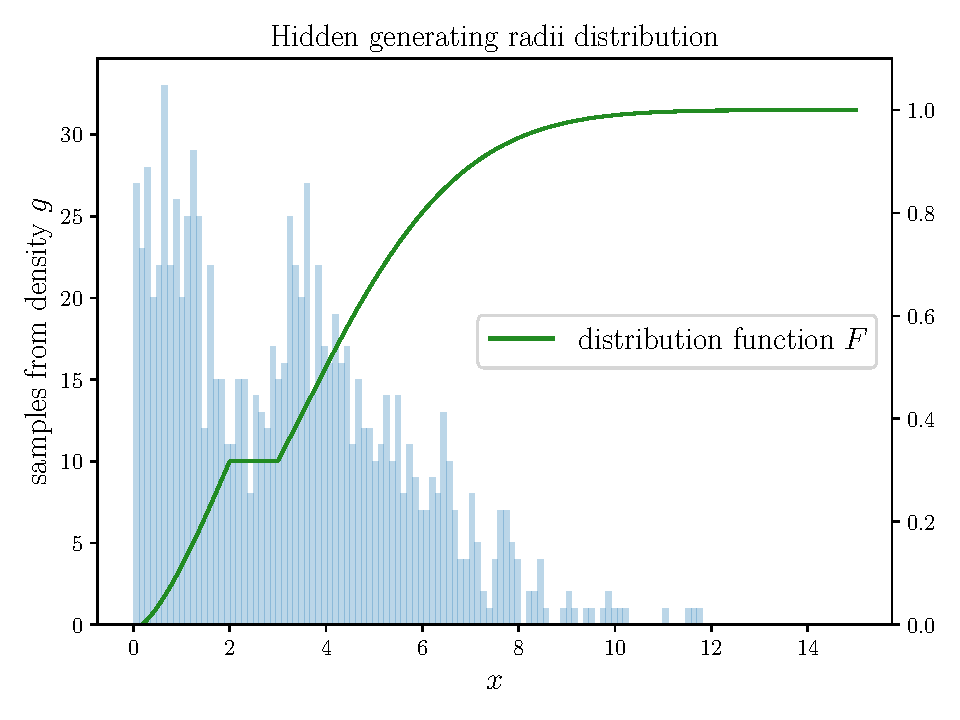
\includegraphics[width=6.4cm]{./img/cdf_truth.pdf}
        \label{fig:image11}
    \end{minipage}
    \hfill
    \begin{minipage}[b]{0.45\textwidth} % Adjust the width as needed
        \centering
        \raisebox{3.1cm}{ % Adjust the value here to move the formula up
        \resizebox{\columnwidth}{!}{%
            \begin{minipage}{\textwidth}
                \begin{align*}
                    &F(x) = \begin{cases}
                        1 - e^{-x^2/20}, & 0 \leq x < 2 \\
                        1 - e^{-1/5}, & x \in [2,3] \\
                        1 - e^{-(x-1)^2/20}, & x > 3
                    \end{cases}
                    \\
                    &g_{\scriptscriptstyle{V}}(x) = \frac{1}{2m_0} \int_{x}^{M} \frac{s e^{-\frac{s^2}{10}} \ind_{[0,2]}(s)}{10\sqrt{s - x}} \, ds \\
                    &\hspace{-0.2cm}+ \frac{1}{2m_0} \int_{x}^{M} \frac{(s-1)e^{-\frac{(s-1)^2}{20}} \ind_{[3,M]}(s)} {10\sqrt{s - x}} \, ds
                \end{align*}
            \end{minipage}}
        }
    \end{minipage}
    \vspace{-0.8cm} % Adjust the value here to decrease the space
    \caption{Underlying cdf $F^*$ and in light blue a histogram of a sample of size $1000$ from $g$.}\label{img: cdf1}
    \vspace{-0.5cm}
    \label{fig:both_images1}
\end{figure}

  
In Figure \ref{img: histograms}, we observe that the distributions of $\sqrt{n} (V^{(\ubar{x},\bar{x})}_n(x)-V(x) )$ and $\sqrt{n} (\hat{V}_n(x)-V(x) )$ closely resemble each other. Moreover, we observe a strong resemblance not only between the estimators but also between their respective limiting distributions, $L_x$ and $N(0,\sigma^2_{\ubar{x},\bar{x}})$. However, the violin plot with the standard percentiles, the second histogram with $\sqrt{n}(\hat{V}_n(x) - V^{(\ubar{x},\bar{x})}_n(x))$ and $W$ and Table \ref{tab: 1} indicate that the variance of $\hat{V}_n(x)$ is slightly bigger than the one of $V^{(\ubar{x},\bar{x})}_n(x)$. 

\begin{figure}[htbp]
    \centering
    \vspace{-0.1cm} 
    \begin{minipage}[b]{0.45\textwidth} % Adjust the width as needed
        \centering
        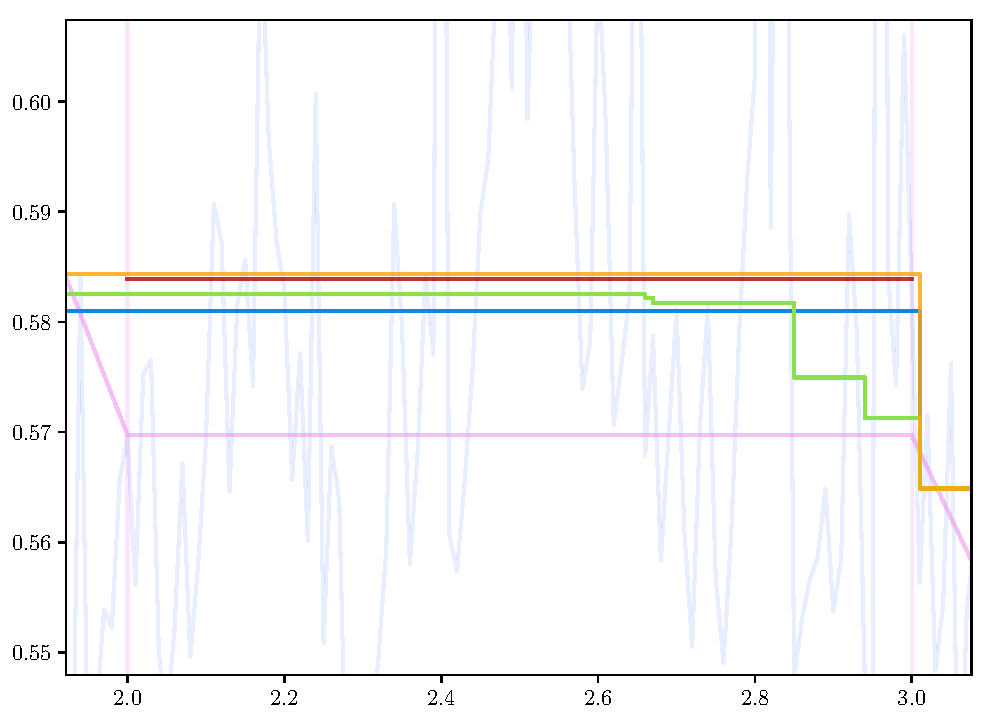
\includegraphics[width = 6.8cm]{img/estimators.pdf}
        \label{fig:image1}
    \end{minipage}
    \hfill
    \begin{minipage}[b]{0.45\textwidth} % Adjust the width as needed
        \centering
        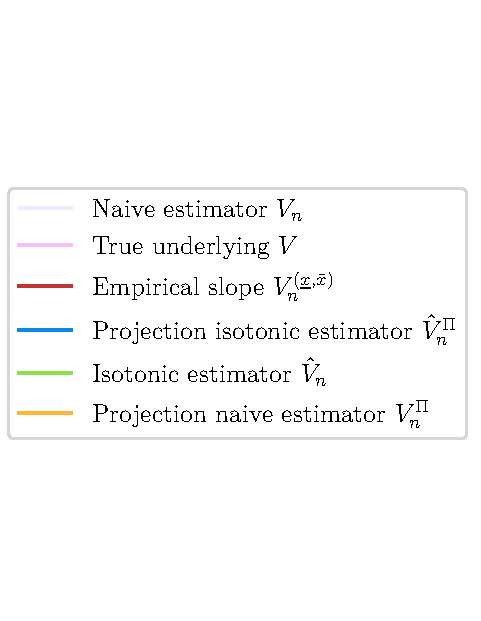
\includegraphics[width = 4.3cm]{img/label_estimators.pdf}
        \label{fig:image2}
    \end{minipage}
    \vspace{-0.6cm} % Adjust the value here to decrease the space
    \caption{All estimators and the true function $V$, which is constant on $[2,3]$, for a sample of size $n=300$.}\label{img: difference all estimators}
    \vspace{-0.1cm}
    \label{fig:both_images}
\end{figure}


The values in Table \ref{tab: 1} were computed using varying sample size $n$ from $g$ as indicated, with $2000$ samples from  $\hat{V}_n(x)$ and $V^{(\ubar{x},\bar{x})}_n(x)$. All the Kernel Density Estimator plots were computed using Scott's rule (where the bin size $h \sim 3.5 \hat{\sigma} n^{-1/3}$) for the chosen bandwidth. For $W$ and $L_x$, $20000$ samples were used.  Taken together, the simulation study confirms the theoretical findings of Theorem \ref{thm: distrib flat F at x total} and \ref{thm: LAM 1}: the informed estimators are efficient and not asymptotically equivalent to the IIE. However, the empirical performances of $V_n^{(\ubar{x},\bar{x})}$ and $\hat{V}_n$ show a high degree of proximity in the estimation scenario where the underlying function $V$ is constant on an interval. Even if $\hat{V}_n$ is used in cases where it is indeed true that $V$ is constant within an interval, the incurred loss appears to be small.


\begin{figure}[H]
    \centering
    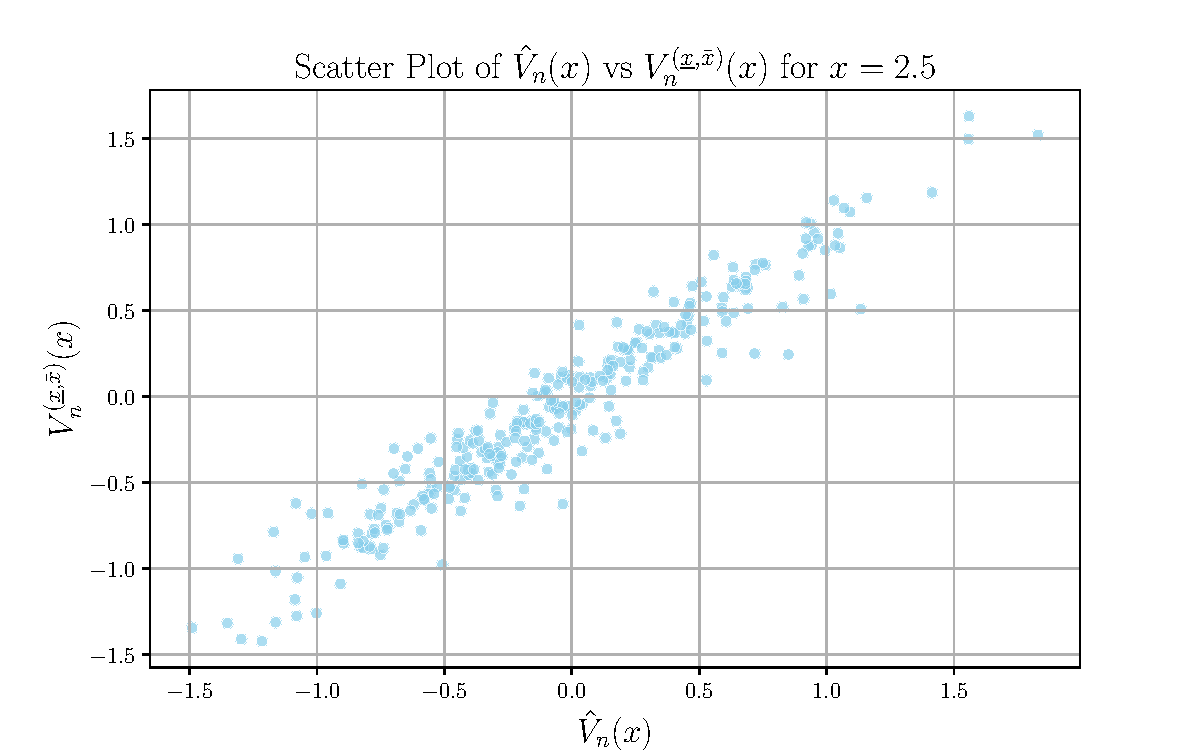
\includegraphics[width=6.5cm]{img/scatterplot1.pdf}
    \hspace{-0.8cm}
    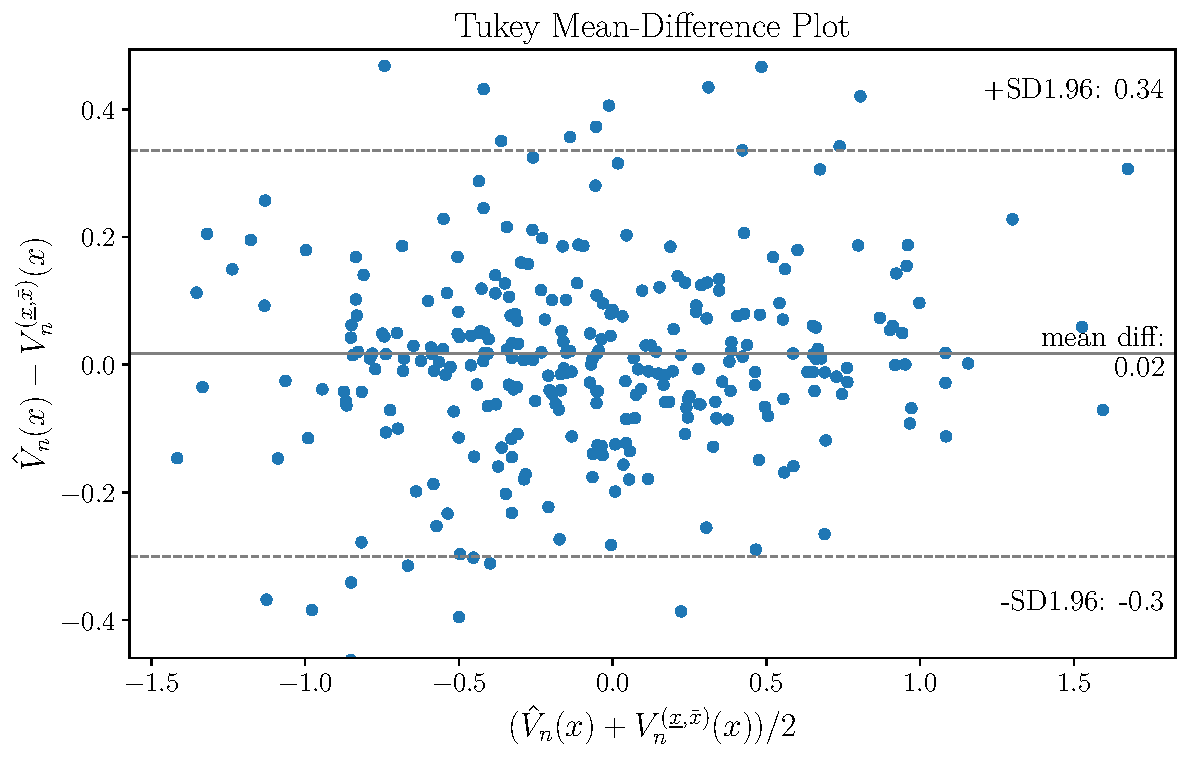
\includegraphics[width=6cm]{img/tukey1.pdf}
    \setlength{\belowcaptionskip}{-6pt}
    \caption{Scatter and Tukey mean-difference plots for $n=1000$ and $300$ repetitions of $\hat{V}_n$ and $V^{(\underline{x},\overline{x})}_n.$}\label{img: scatter + tuckey}
  \end{figure}
\begin{figure}[H]
    \centering
    \vspace{-0.2cm}
    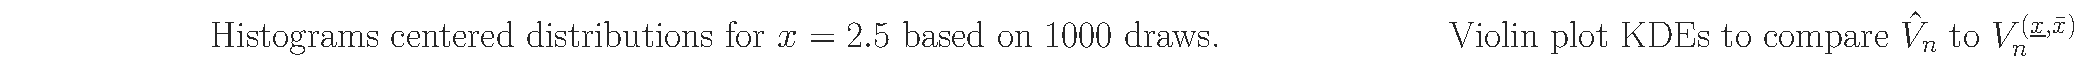
\includegraphics[width=12.1cm]{img/title_histo.pdf}
    \vspace{-0.05cm} 
    
    \begin{minipage}[b]{\linewidth}
      \centering
      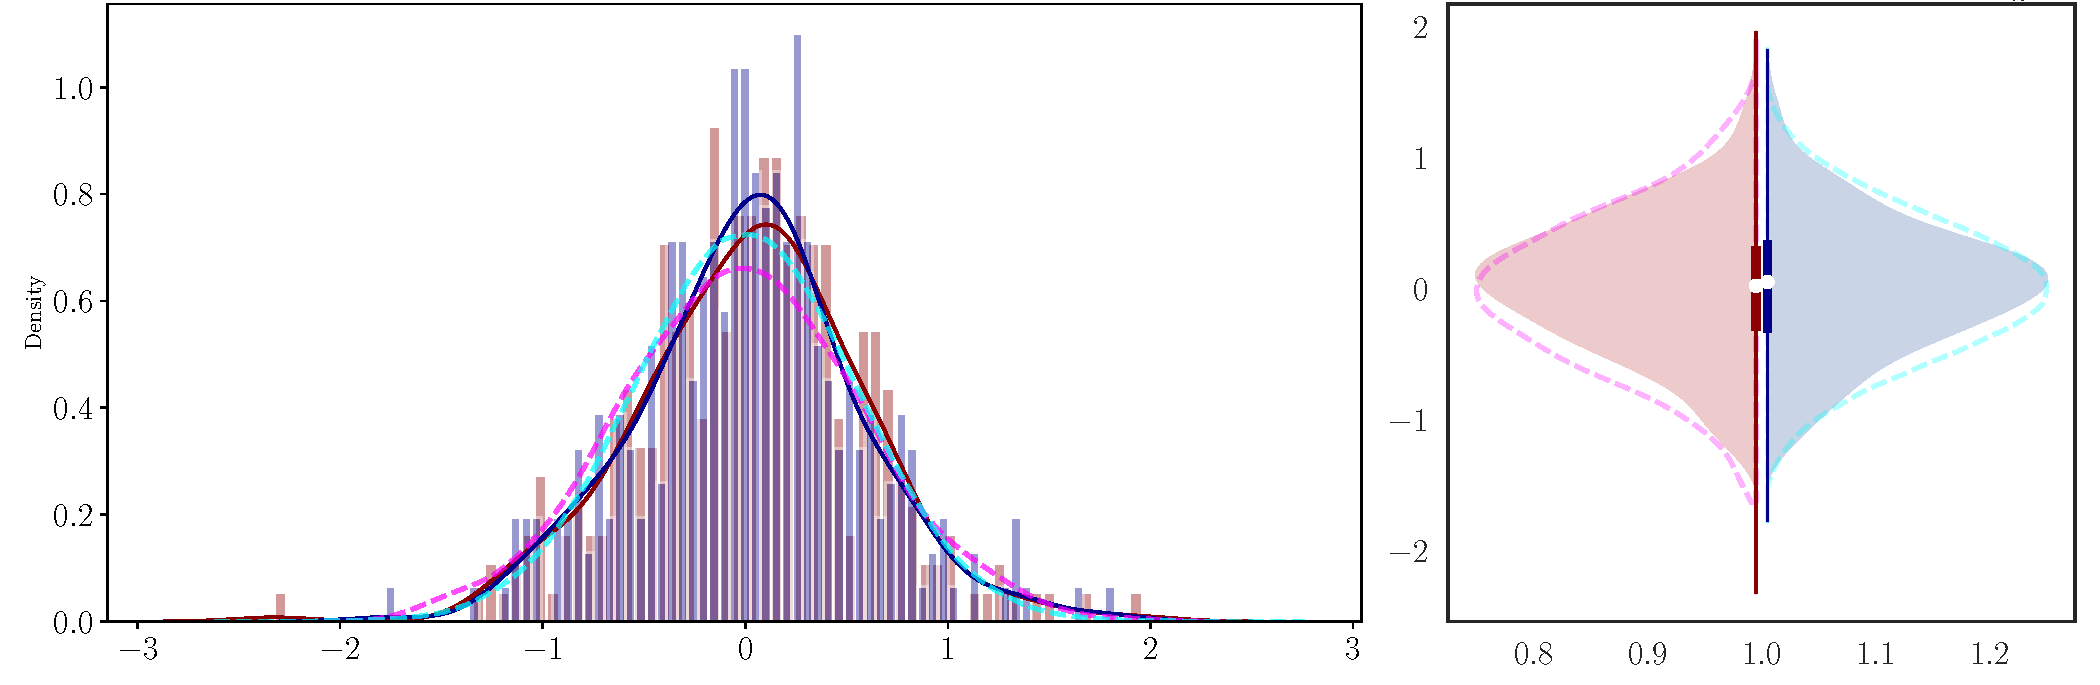
\includegraphics[width=12.1cm]{img/1000_3cropped1.pdf}
    \end{minipage}
  
  \end{figure}
  \begin{figure}[H]
      \centering
      \begin{minipage}[b]{0.45\textwidth} % Adjust the width as needed
          \centering
          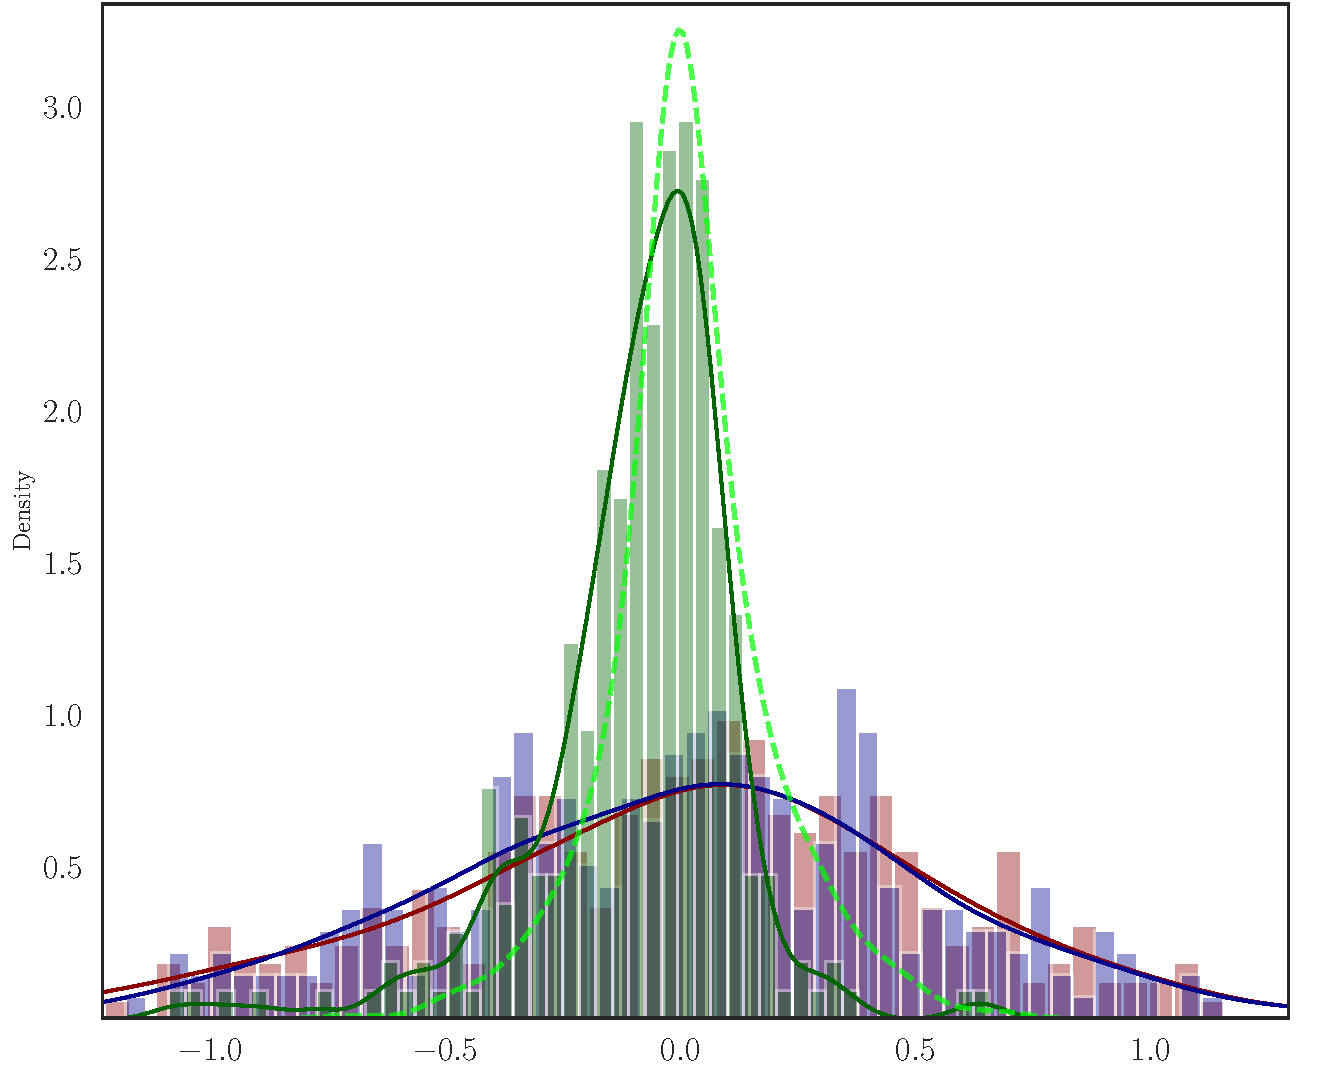
\includegraphics[width=7.2cm]{img/W52cropped.pdf}
          %\caption{First image}\label{fig:image1}
      \end{minipage}
      \hspace{0.8cm}
      \begin{minipage}[b]{0.45\textwidth} % Adjust the width as needed
          \centering
          \raisebox{2.5cm}{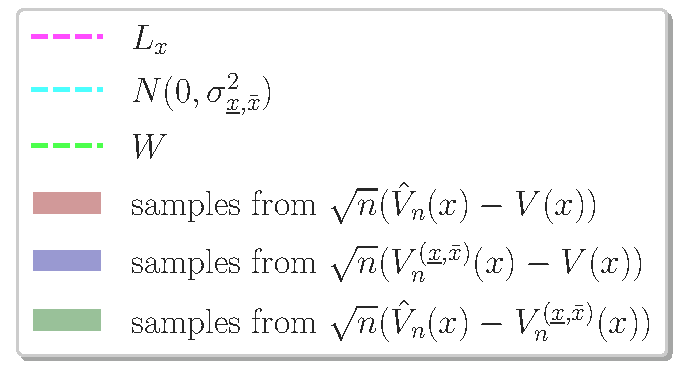
\includegraphics[width=4.2cm]{img/labelextracthisto.pdf}}
          %\caption{Second image}\label{fig:image2}
      \end{minipage}
      \caption{Based on $1000$ samples from $g$, centered and rescaled histograms based on $300$ repetitions, $V^{(\underline{x},\overline{x})}_n$ and their difference compared with respective limiting distributions $L_x$, $N(0,\sigma^2_{\underline{x},\overline{x}}) $ and $W$.}\label{img: histograms}
  \end{figure}




\begin{table}[H]
    \centering
    \resizebox{\columnwidth}{!}{%
    \begin{tabular}{|c|c c c c c||c|c|}
        \hline
         $n$ & 100 & 200 & 400 & 1000 & 2000  &  & limit \\
        \hline
         $\sqrt{n}(V^{(\ubar{x},\bar{x})}_n-V )(x)$ & 0.5441 & 0.5439 & 0.5465 & 0.5467 & 0.5464 & $N(0,\sigma^2_{\ubar{x},\bar{x}})$ & 0.5466 \\
        \hline
         $\sqrt{n} (\hat{V}_n-V)(x)$ & 0.5537 &  0.5592 & 0.5627 & 0.5664 & 0.5697  & $L_x$ & 0.5703 \\
        \hline
    \end{tabular}
    }
    \caption{Standard deviations}
    \label{tab: 1}
\end{table}

\vspace{-1cm}
\subsection{Conclusion}
We conclude by stressing the fact that the local asymptotically minimax variance in Theorem \ref{thm: LAM 1} coincides with the one obtained in Theorem \ref{thm: distrib flat F at x total 2}. This shows that in the setting in which $V$ is constant on $[\ubar{x},\bar{x}]$, for $\ubar{x} < \bar{x}$, the informed estimators are asymptotically efficient, whereas the isotonic inverse estimator is not, as it is clearly shown by Theorem \ref{thm: LAM 1}. However, we conjecture that the isotonic estimator remains asymptotically efficient in the situations in which the boundary points $\ubar{x},\bar{x}$ are allowed to converge to $x$ at an arbitrarily polynomial rate (or slower). In this case, the rate of convergence drops to $\sqrt{n/\log{(\bar{x}-\ubar{x})^{-1}}}$. 

From a practical point of view, both the results of the current section and Theorems \ref{thm: distrib flat F at x}-\ref{thm: normality Holder} are difficult to use to obtain confidence bands, as they require estimating the density \( g \), either at $x$ or globally to compute $\sigma^2_{\ubar{x},\bar{x}}$ or to compute the covariance structure of the limiting Gaussian process. We envision Theorems \ref{thm: distrib flat F at x}-\ref{thm: normality Holder} and the asymptotic results of the current section as the theoretical foundation, while the practical computation of confidence bands may be better addressed through bootstrap methods. A potential direction for further research would be proving formally why the bootstrap works. We believe that a formal justification would combine our theoretical results with the techniques used in \cite{19} (which already shows consistency of the bootstrap for $\gamma =1$ in the limiting variance of Theorem \ref{thm: distrib flat F at x}). 

Another potential direction for further investigation is whether the IIE is efficient in the setting in which there exists an interval of constancy for $V$ but the boundary points $\ubar{x},\bar{x}$ are unknown. However, the definition and assessment of \textit{efficiency} in this context are unclear. For practical purposes, if the boundary points $\ubar{x},\bar{x}$ are unknown, the IIE remains the state-of-art as it behaves very closely to the efficient estimator and in the $\sqrt{n / \log{n}}$ rate setting is efficient and adaptive to the level of smoothness of $V$.


\section{Appendix}\label{sec: appendix chapter2}  % Use * to avoid automatic numbering

\subsection{Proofs of complemental statements for Theorem \ref{thm: normality Holder}.}\label{subsec: proofs lemmas thm normality holder}%% if no title is needed, leave empty \section*{}.
First we provide some proofs about the fundamental behavior of the covariance structure of the process $Z_n(t)$. We start by showing the case of the variance and we will proceed by giving a proof along the same lines of \eqref{eq: covariance structure final}. We will use several times how samples of $Z$ with density $g$ (see \eqref{eq: density of the observations}) are obtained in Wicksell's problem. First, note that the observable radii in the cross sections cannot exceed the radii of the associated sphere; the spheres with bigger radius are more likely to be sampled. Thus the distribution of the squared radii of the spheres actually cut is not $F^*$ but a biased version of it; thus we write $X$ with distribution function $F$ for the squared radius of the spheres actually cut. Since we assume the samples are gathered uniformly, the observed squared circle radius $Z$ is related to $X$ via:
\begin{align}\label{eq: sampling of Z}
    Z = (1-U^2) X = V X, \quad U \sim U[0,1], \quad V \sim \mathrm{Be}(1,1/2)
\end{align}

\begin{lemma}\label{lemma: variance without assum. g}
Fix $x >0$. If $g(x) < \infty$, then:
\begin{align*}
    \ex \left(\sqrt{Z-x} \ind_{\{Z>x\}}-\sqrt{Z-x-\varepsilon} \ind_{\{Z>x+\varepsilon\}}\right)^2 \sim \varepsilon^2 \log \left( \frac{1}{\varepsilon} \right) g (x), \quad \text{as} \quad \varepsilon \downarrow 0.
\end{align*}
\end{lemma}
\begin{proof}
Define $Z_x := Z-x$. The left side is: 
\begin{align*}
\underbrace{\ex Z_x \ind_{\{ Z_x < \varepsilon \}}}_{(1)} + \underbrace{\ex \left(\sqrt{Z_x} - \sqrt{Z_x - \varepsilon} \right)^2 \ind_{\left\{ Z_x > \varepsilon \right\}}}_{(2)}. 
\end{align*}
We start with $(1)$. By making a substitution below with $vX - x = y(X-x)$, which means $1-v = (1-y)\frac{X-x}{X}$, we obtain:
\begin{align*}
   \ex  \, Z_x \ind_{Z_x < \varepsilon}  &\stackrel{\eqref{eq: sampling of Z}}{=} \ex  \left\{ \ind_{X > x} \int_{0 < vX - x < \varepsilon} (vX -x) \frac{\ind_{0<v<1}}{2 \sqrt{1 - v}} \, dv \right\}  \\
    &\: \: = \ex  \left\{ \ind_{X> x} \int_{0}^{\frac{\varepsilon}{X - x} \wedge 1} \frac{y}{2 \sqrt{1-y}} \frac{(X-x)^{3/2}}{\sqrt{X}} \, dy\right\}.
\end{align*}
If we define $y(z) = \int_{0}^{z} \frac{y}{2 \sqrt{1-y}} \, dy$ then the above equals to:
\begin{align*}
    \ex  \left\{  y\left(\frac{\varepsilon}{X - x} \wedge 1 \right) \ind_{X> x} \frac{(X-x)^{3/2}}{\sqrt{X}} \right\}.
\end{align*}
Using: $\int \frac{y}{2 \sqrt{1-y}} \, dy = \frac{(1-y)^{3/2}}{3} - \sqrt{1-y} + c$, we can see that:
\begin{align*}
    y\left(\frac{\varepsilon}{X - x} \wedge 1\right) &= \int_{0}^{\frac{\varepsilon}{X - x} \wedge 1} \frac{y}{2 \sqrt{1-y}} \, dy =  \frac{1}{4} \left( \frac{\varepsilon}{X-x} \right)^2 + O\left( \left( \frac{\varepsilon}{X-x} \right)^3 \right).
\end{align*}
Moreover it is also true $y(z) \leq z^2, \: \: \forall \: z \in (0,1)$. The above proves:
\begin{align}\label{eq: EZa less equal}
\ex \, Z_x \ind_{Z_x < \varepsilon} = O(\varepsilon^2).     
\end{align}
Therefore $(1)$ is negligible. Now we proceed with $(2)$. Using Taylor's theorem with integral form of the remainder we obtain:
\begin{align*}
    &\ex \left( \sqrt{Z_x} - \sqrt{Z_x - \varepsilon} \right)^2 \ind_{\{ Z_x > \varepsilon \}} =  \ex  \int_{0}^{1} \int_{0}^{1} \frac{\varepsilon}{2 \sqrt{Z_x - \varepsilon s}} \frac{\varepsilon}{2 \sqrt{Z_x - \varepsilon t}} \, ds \, dt \, \ind_{\{Z_x > \varepsilon \}} \\
    &\stackrel{\eqref{eq: sampling of Z}}{=} \ex  \int_{0}^{1} \int_{0}^{1} \int_{0}^{1} \frac{\varepsilon}{2 \sqrt{vX-x - \varepsilon s}} \frac{\varepsilon}{2 \sqrt{v X - x - \varepsilon t}} \frac{1}{2 \sqrt{1-v}} \ind_{\{vX - x > \varepsilon \}} \, dv \, ds \, dt.
\end{align*}
Now we use again the substitution $vX - x = y(X-x)$ which implies $1-v = (1-y) \frac{X-x}{X}$ and $y(\varepsilon,s,t) = \int_{\varepsilon}^{1} \frac{1}{\sqrt{y - \varepsilon s}} \frac{1}{\sqrt{y - \varepsilon t}} \frac{1}{\sqrt{1-y}} \, dy$ to obtain:
\begin{align*}
    &= \frac{\varepsilon^2}{8} \ex  \int_{0}^{1} \int_{0}^{1} \int_{0}^{1} \frac{1}{\sqrt{y - \frac{\varepsilon s}{X-x}}} \frac{1}{\sqrt{y - \frac{\varepsilon t}{X-x}}} \frac{1}{ \sqrt{1-y}} \frac{\ind_{\{y(X - x) > \varepsilon \}}}{\sqrt{X-x} \sqrt{X}} \, dy \, ds \, dt \\
    &= \frac{\varepsilon^2}{8} \ex  \int_{0}^{1} \int_{0}^{1} y\left( \frac{\varepsilon}{X-x},s,t \right) \frac{\ind_{\{X - x > \varepsilon \}}}{\sqrt{X-x} \sqrt{X}} \, ds \, dt.
\end{align*}
Now we show the two following relations $\forall \: 0 < \varepsilon,s,t < 1$:
\begin{align}
    &y(\varepsilon,s,t) \sim \log{\frac{1}{\varepsilon}} - \frac{1}{2}\log{\log{\frac{1}{\varepsilon}}} + O(1) \quad \text{as} \: \varepsilon \downarrow 0 \label{eq: relations on y} \\
    & y(\varepsilon,s,t) \leq \left( \log{\frac{1}{\varepsilon}} + \log{\frac{e^2}{1 - s \vee t}}\right) \frac{1}{\sqrt{1 - s \vee t}} + 1. \label{eq: relations on y 2}
\end{align}
From this it will follow that:
\begin{align}\label{eq: essential second moment rel variance}
    \ex \left( \sqrt{Z_x} - \sqrt{Z_x - \varepsilon} \right)^2 \ind_{\{ Z_x > \varepsilon \}} \sim \frac{\varepsilon^2}{4} g(x) \log{\frac{1}{\varepsilon}}. 
\end{align}
Fix $\varepsilon < b < 1$, then we can split the integral in the definition of $y(\varepsilon,s,t)$ into two integrals: one from $\varepsilon$ to $b$ and another one from $b$ to $1$. Let us look at the second one:
\begin{align*}
    \int_{b}^1 \frac{(1-y)^{-\frac{1}{2}}}{y \sqrt{y - \varepsilon s}} \frac{y}{\sqrt{y - \varepsilon t}} \, dy \leq& \frac{b}{b - \varepsilon} \int_{b}^1 \frac{1}{y \sqrt{1-y}} \, dy = \frac{b}{b - \varepsilon} 2 \tanh^{-1} (\sqrt{1-b}). 
\end{align*}
Here we used the fact that the mapping $y \mapsto \frac{y}{y-\varepsilon s}$ is decreasing on $[\varepsilon s,1]$, that $\frac{b}{b - \varepsilon s} \leq \frac{b}{b - \varepsilon}$ and $\int \frac{1}{y} \frac{1}{\sqrt{1-y}} \, dy = -2 \tanh^{-1}(\sqrt{1-y}) + c$. This shows that the asymptotic behavior will be determined by the integral between $\varepsilon$ and $b$;
\begin{align*}
    &\bigg| \int_{\varepsilon}^{b} \frac{1}{\sqrt{y - \varepsilon s}} \frac{1}{\sqrt{y - \varepsilon t}} \frac{1}{\sqrt{1 - y}} \, dy - \int_{\varepsilon}^{b} \frac{1}{\sqrt{y - \varepsilon s}} \frac{1}{\sqrt{y - \varepsilon t}} \, dy \bigg| \\
    &\quad \quad \quad \leq \int_{\varepsilon}^{b} \frac{1}{\sqrt{y - \varepsilon s}} \frac{1}{\sqrt{y - \varepsilon t}} \, dy \left( \frac{1}{\sqrt{1-b}} -1 \right).
\end{align*}
On the other hand, since:
\begin{align*}
\int_{\varepsilon}^b \frac{1}{y-\varepsilon s \wedge t} \, d y \leqslant \int_{\varepsilon}^b \frac{1}{\sqrt{y-\varepsilon s}} \frac{1}{\sqrt{y-\varepsilon t}} \, d y \leqslant  \int_{\varepsilon}^b \frac{1}{y-\varepsilon s \vee t} \, d y.
\end{align*}
Therefore we have:
\begin{align*}
    \int_{\varepsilon}^{b} \frac{1}{\sqrt{y - \varepsilon s}} \frac{1}{\sqrt{y - \varepsilon t}} \frac{1}{\sqrt{1 - y}} \, dy 
    \begin{cases}
        \leq \log{\left\{ \frac{b - \varepsilon s \vee t}{\varepsilon (1 - s \vee t)} \right\}} \frac{1}{\sqrt{1-b}}, \\ 
        \geq \log{\left\{ \frac{b - \varepsilon s \wedge t}{\varepsilon (1 -  s \wedge t)} \right\}}\left(2 - \frac{1}{\sqrt{1-b}} \right).
    \end{cases}
\end{align*}
Using $b = \frac{1}{\sqrt{\log{\frac{1}{\varepsilon}}}}$ we obtain for fixed $c$: 
\begin{align*}
    \log{\left\{ \frac{1/\sqrt{\log{\frac{1}{\varepsilon}}} - \varepsilon c}{\varepsilon (1-c)} \right\}} &= \log{\left\{ 1 - \varepsilon \sqrt{\log{\frac{1}{\varepsilon}}} c\right\}} + \log{\left\{ \frac{1}{\sqrt{\log{\frac{1}{\varepsilon}}}} \right\}} + \log{\frac{1}{\varepsilon}} + \\ 
    &\quad + \log{\frac{1}{1-c}} \sim \log{\frac{1}{\varepsilon}} - \frac{1}{2} \log{\log{\frac{1}{\varepsilon}}} + O(1), \quad \quad \text{as} \: \: \varepsilon \downarrow 0.
\end{align*}
This proves the first relation \eqref{eq: relations on y}. Now we proceed with relation \eqref{eq: relations on y 2}. Assume $s \leq t$. By performing a substitution $y - \varepsilon t = z (1 - \varepsilon t)$ which means $1 - y = (1 - \varepsilon t)(1 - z)$ we obtain:
\begin{align*}
    y(\varepsilon,s,t) \leq \int_{\varepsilon}^1 \frac{1}{y - \varepsilon t} \frac{1}{\sqrt{1 - y}} \, dy = \frac{1}{\sqrt{1 - \varepsilon t}} \int_{\frac{\varepsilon (1-t)}{1-\varepsilon t}}^{1} \frac{1}{z} \frac{1}{\sqrt{1-z}} \, dz. 
\end{align*}
We used that we can compute the primitive: $\int \frac{1}{y} \frac{1}{\sqrt{1-y}} \, dy = -2 \tanh^{-1}(\sqrt{1-y}) + c$. Therefore:
\begin{align*}
     &\frac{1}{\sqrt{1 - \varepsilon t}}  \int_{\frac{\varepsilon (1-t)}{1-\varepsilon t}}^{1} \frac{1}{z} \frac{1}{\sqrt{1-z}} \, dz = 2 \tanh^{-1}\left( \sqrt{1 - \frac{\varepsilon (1-t)}{1 - \varepsilon t}}\right) \frac{1}{\sqrt{1 - \varepsilon t}}   \\
     & = \frac{1}{\sqrt{1 - \varepsilon t}} \log{\left\{ \frac{1 +  \sqrt{\frac{1 - \varepsilon}{1 - \varepsilon t}} }{ 1 - \sqrt{\frac{1 - \varepsilon}{1 - \varepsilon t}}} \right\}}  = \log{\left\{ \frac{\left(\sqrt{1 - \varepsilon t} + \sqrt{1 - \varepsilon}\right)^2}{\varepsilon - \varepsilon t} \right\}} \frac{1}{\sqrt{1 - \varepsilon t}}  \\
     & \leq \bigg( \log{\frac{1}{\varepsilon}} + \log{\frac{1 - \varepsilon t}{1-t}} + 2\bigg) \frac{1}{\sqrt{1 - \varepsilon t}} \leq \left( \log{\frac{1}{\varepsilon}} + \log{\frac{e^2}{1-t}} \right) \frac{1}{\sqrt{1 - t}} +1.
\end{align*}
And this proves \eqref{eq: relations on y 2}. Now we proceed by using the two relations we just proved. First of all,  \eqref{eq: relations on y} as $\varepsilon \downarrow 0$:
\begin{align*}
    &\frac{y\left( \frac{\varepsilon}{X_x}, s, t \right) \ind_{\{X_x > \varepsilon \}}}{\log{\frac{1}{\varepsilon}}} = \frac{y\left( \frac{\varepsilon}{X_x}, s, t \right) \ind_{\{X_x > \varepsilon \}}}{\log{\frac{X_x}{\varepsilon}}} \cdot \frac{\log{X_x}  + \log{\frac{1}{\varepsilon}}}{\log{\frac{1}{\varepsilon}}} \rightarrow \ind_{\{ X > x\}}
\end{align*}
Now using $\log{xy} \leq \log{x} \ind_{x> 1} + \log{y}$ and \eqref{eq: relations on y 2} we obtain:
\begin{align*}
    \frac{y\left( \frac{\varepsilon}{X-x}, s,t \right) \mathbf{1}_{\{ X-x > \varepsilon\}}}{ \log{\frac{1}{\varepsilon}}} &\leq \frac{\left( \log{\frac{X_x}{\varepsilon}} + \log{\frac{e^2}{1 - s \vee t}} \right) \frac{1}{\sqrt{1 - s \vee t}} + 1}{\log{\frac{1}{\varepsilon}}} \\ 
    &\lesssim \left( \log{X_x} \ind_{X_x > 1} + \log{\frac{e^2}{\sqrt{1 - s \vee t}}}\right) \frac{1}{\sqrt{1 - s \vee t}} + 1.
\end{align*}
Since the idea is to apply the Dominated Convergence Theorem to:
\begin{align*}
    \frac{1}{\log{\frac{1}{\varepsilon}}} \ex  \int_{0}^{1} \int_{0}^{1} y\left( \frac{\varepsilon}{X-x},s,t \right) \frac{1}{2\sqrt{X-x} \sqrt{X}} \ind_{\{X - x > \varepsilon \}} \: ds \: dt,
\end{align*}
we need to verify that all the upper bounds have finite expectations. First $\frac{\log{X_x}\ind_{\{ X_x > 1\}}}{\sqrt{X}} \lesssim 1$ which means:
\begin{align*}
    \int_{0}^{1} \int_{0}^{1} \frac{\log{X_x} \ind_{\{X_x > 1\}} }{\sqrt{X}} \frac{1}{\sqrt{1 - s \vee t}} \, ds \, dt \lesssim 2 \int_{0}^{1} \int_{0}^{t} \frac{1}{\sqrt{1-t}} \, ds \, dt < \infty.
\end{align*}
On the other hand:
\begin{align*}
    &\int_{0}^{1} \int_{0}^{1} \left( \log{\frac{1}{1 - s \vee t}} \right) \frac{1}{\sqrt{1 - s \vee t}} \, ds \, dt \lesssim 2 \int_{0}^{1} \int_{0}^{t} \left( \log{\frac{1}{1 - t}}\right) \frac{1}{\sqrt{1-t}} \, ds \, dt \\
    &\quad \quad = 2 \int_{0}^{1} t \left( \log{\frac{1}{1-t}} \right) \frac{1}{\sqrt{1-t}} \, dt < \infty.
\end{align*}
So by the Dominated Convergence Theorem, if $g(x)= \ex  \frac{1}{2 \sqrt{X-x}} \frac{1}{\sqrt{X}} \ind_{\{X>x \}} < \infty$ we obtain the claim.
\end{proof}

\begin{proof}[\hypertarget{proof of lemma 1}{\textbf{Proof of}} \eqref{eq: covariance structure final}]
Fix $s, t \in I_x$. Take the case $0 \leq s \leq t$. Fix $\mu$; we define the function $\phi(\cdot, \mu)$ as follows:
$$
\phi(z, \mu)=\sqrt{z-x} \, \ind_{[x, \infty)}(z)-\sqrt{z-x-\mu} \, \ind_{[x+\mu, \infty)}(z) .
$$
Using the i.i.d.\ property, we can write:
\begin{align}\label{eq: equation covariance}
\operatorname{Cov}\left(Z_n(s), Z_n(t)\right)= 4 \delta_n^{-2} ( \delta^*_n)^{-2}  n^{-1} \operatorname{Cov}\left(\phi\left(Z, \delta^*_n t\right), \phi\left(Z, \delta^*_n s\right)\right),
\end{align}
where $Z$ has density $g$. 
Since $g(x) < \infty$, we will prove:
\begin{align}\label{eq: covariance phi function new}
\ex  \phi\left(Z, \delta^*_n s\right) \phi\left(Z, \delta^*_n t\right)=- \frac{1}{4}st g(x) (\delta^*_n)^2 \log{\delta^*_n} +O\left((\delta^*_n)^2 \right),
\end{align}
which implies \eqref{eq: covariance structure final} for $\delta_n=n^{-1 / 2} \sqrt{\log n}$ and $\delta^*_n = (\delta_n)^{1/\gamma_x}$. Define $Z_x := Z-x$:
\begin{align*}
    &\ex \left[ \sqrt{Z_x} \ind_{\{Z_x > 0 \}} - \sqrt{Z_x - \delta^*_n t} \ind_{\{Z_x > \delta^*_n t \}} \right] \hspace{-0.1cm} \left[ \sqrt{Z_x} \ind_{\{Z_x > 0 \}} - \sqrt{Z_x - \delta^*_n s} \ind_{\{Z_x > \delta^*_n s \}} \right]\\
    &= \underbrace{\ex  Z_x \ind_{\{ 0 < Z_x < \delta^*_n s\}}}_{(1)} + \underbrace{\ex  \left\{ \sqrt{Z_x} \left(\sqrt{Z_x} - \sqrt{Z_x - \delta^*_n s} \right) \ind_{\{ \delta^*_n s \leq Z_x \leq \delta^*_n t\}}\right\}}_{(2)} + \\
    &\quad + \underbrace{\ex \left\{\left( \sqrt{Z_x} - \sqrt{Z_x - \delta^*_n t} \right) \left( \sqrt{Z_x} - \sqrt{Z_x - \delta^*_n s} \right) \ind_{\{Z_x >  \delta^*_n t \}} \right\}}_{(3)}.
\end{align*}
Let us start with $(1)$. We can use \eqref{eq: EZa less equal} to see that for $\delta^*_n$ going to zero: 
\begin{align*}
    \ex  Z_x \ind_{\{0 < Z_x < \delta^*_n s \}} \leq (\delta^*_n s)^2 \ex  \frac{1}{\sqrt{X-x}} \frac{1}{\sqrt{X}} \ind_{\{ X > x\}} = O((\delta^*_n s)^2).
\end{align*}
This shows that this term is negligible as for the covariance it is multiplied by $4 \delta_n^{-2} ( \delta^*_n)^{-2}  n^{-1} = 4 \frac{1}{\log{n}} ( \delta^*_n)^{-2}$, will be of order $\frac{1}{\log{n}}$ and it will go to zero. \\
Let us continue with $(2)$. First note one can upper bound $(2)$ using Hölder's inequality and notice that by \eqref{eq: essential second moment rel variance} we have:
\begin{align}\label{eq: symmetric case moment squared}
    \ex  \left( \sqrt{Z_x} - \sqrt{Z_x - \delta^*_n s}\right)^2 \ind_{\{ Z_x > \delta^*_n s \}} \sim \frac{(\delta^*_n s)^2}{4} \log{\frac{1}{\delta^*_n s}} g(x).
\end{align}
Which implies that the square root of this term is of the order $O(\delta^*_n \sqrt{\log{\frac{1}{\delta^*_n}}})$. Moreover, notice that by \eqref{eq: EZa less equal}:
\begin{align*}
    \left\{ \ex  Z_x \ind_{\{ \delta^*_n s < Z_x < \delta^*_n t \}} \right\}^{1/2} \leq \left\{ \ex  Z_x \ind_{\{  Z_x > \delta^*_n s \}} \right\}^{1/2} = O(\delta^*_n ).
\end{align*}
All together we obtain that $(2)$ is of the order $O((\delta^*_n)^2 \sqrt{\log{(\delta^*_n})^{-1}})$. This quantity for the covariance structure will be multiplied by $4 \delta_n^{-2} ( \delta^*_n)^{-2}  n^{-1}$, and will be of order $O(\frac{1}{\sqrt{\log{n}}})$ thus it will go to zero because $\sqrt{\log{\frac{1}{\delta^*_n}}} \sim \sqrt{\log{n}}$. \\
Now we argue the order of $(3)$. We argue like in the proof of \eqref{eq: essential second moment rel variance}:
\begin{align*}
    (3) &= (\delta^*_n)^2 st \ex  \int_{0}^{1} \int_{0}^{1} \frac{1}{2 \sqrt{Z_x - \delta^*_n s p}} \frac{1}{2 \sqrt{Z_x - \delta^*_n t q}} \, dp \,dq \: \ind_{\{Z_x > \delta^*_n t\}} \\
    &=  \ex  \int_{0}^{1} \int_{0}^{1} \int_{0}^{1} \frac{(\delta^*_n)^2 st}{2 \sqrt{vX-x - \delta^*_n s p}} \frac{\ind_{\{vX - x > \delta^*_n t\}}}{2 \sqrt{v X - x - \delta^*_n t q}} \frac{1}{2 \sqrt{1-v}} \, dv \, dp \, dq.
\end{align*}
Now we use again the substitution $vX - x = y(X-x)$ which implies $1-v = (1-y) \frac{X-x}{X}$ and $y(\delta^*_n,s,t) = \int_{\delta^*_n}^{1} \frac{1}{\sqrt{y - \delta^*_n s}} \frac{1}{\sqrt{y - \delta^*_n t}} \frac{1}{\sqrt{1-y}} dy$ to obtain:
\begin{align*}
    &=\ex  \int_{0}^{1} \int_{0}^{1} \int_{0}^{1} \frac{(\delta^*_n)^2 st}{8 \sqrt{y - \frac{\delta^*_n t}{X-x} q}} \frac{\ind_{\{y(X - x) > \delta^*_n t\}}}{ \sqrt{y - \frac{\delta^*_n s}{X-x} p}} \frac{1}{ \sqrt{1-y}} \frac{1}{\sqrt{X-x} \sqrt{X}} \, dy \, dp \, dq \\
    &= \frac{(\delta^*_n)^2}{8} st \ex  \int_{0}^{1} \int_{0}^{1} y\left( \frac{\delta^*_n}{X-x},sp,tq \right) \frac{1}{\sqrt{X-x} \sqrt{X}} \ind_{\{X - x > \delta^*_n t \}} \, dp \, dq.
\end{align*}
Then one can obtain the claim by using \eqref{eq: relations on y} and \eqref{eq: relations on y 2}. The reason why we can apply the Dominated Convergence theorem is as in the proof of Lemma \ref{lemma: variance without assum. g}. The cases $s \leq 0 \leq t$ and $s \leq t \leq 0$ can be argued in a similar way.
\end{proof}
\begin{comment}
Now assume instead that $s \leq 0 \leq t$:
\begin{align*}
    &\ex\left[ \sqrt{Z_x} \ind_{\{Z_x > 0 \}} - \sqrt{Z_x - \delta^*_n t} \ind_{\{Z_x > \delta^*_n t \}} \right] \left[ \sqrt{Z_x} \ind_{\{Z_x > 0 \}} - \sqrt{Z_x - \delta^*_n s} \ind_{\{Z_x > \delta^*_n s \}} \right] \\
    &= \underbrace{\ex \left\{ \sqrt{Z_x} \left(\sqrt{Z_x} - \sqrt{Z_x - \delta^*_n s} \right)\ind_{\{ 0 \leq Z_x \leq \delta^*_n t\}}\right\}}_{(1)} + \\
    & \quad \quad \quad \quad \quad \quad \quad + \underbrace{\ex\left\{\left( \sqrt{Z_x} - \sqrt{Z_x - \delta^*_n t} \right) \left( \sqrt{Z_x} - \sqrt{Z_x - \delta^*_n s} \right) \ind_{\{Z_x >  \delta^*_n t \}} \right\}}_{(2)}.
\end{align*}
Now the term $(1)$ is non positive. Therefore we have to make sure it will not go to minus infinity once we multiply it by $4 \delta_n^{-2} ( \delta^*_n)^{-2}  n^{-1} = 4 \frac{1}{\log{n}} ( \delta^*_n)^{-2}$, when we look at the covariance structure. Indeed we can lower bound it using again the same reasoning as above with Hölder's inequality and look at the behavior of:
\begin{align*}
    \ex \left\{\left( \sqrt{Z_x - \delta^*_n s} - \sqrt{Z_x} \right)^2 \ind_{Z_x > 0} \right\} = \ex \left\{\left( \sqrt{Z_x} - \sqrt{Z_x + \delta^*_n s} \right)^2 \ind_{Z_x > - \delta^*_n s} \right\}.
\end{align*}
The behavior of the above expression is determined once again by \eqref{eq: essential second moment rel variance}. Therefore $(1)$ is bounded above by $0$ and from below it is of order $O((\delta^*_n)^2 \sqrt{\log{(\delta^*_n)^{-1}}})$. Therefore we conclude that once we multiply it by $4 \delta_n^{-2} ( \delta^*_n)^{-2}  n^{-1}$ it will converge to zero, just like the symmetric case of \eqref{eq: symmetric case moment squared}.\\
Now we determine the behavior of $(2)$. Using the same reasoning as above, we have:
\begin{align*}
    (2) = \frac{(\delta^*_n)^2}{8} st \ex \int_{0}^{1} \int_{0}^{1} y\left( \frac{\delta^*_n}{X-x},sp,tq \right) \frac{1}{\sqrt{X-x} \sqrt{X}} \ind_{\{X - x > \delta^*_n t \}} dp \: dq,
\end{align*}
where: $y(\varepsilon, ps, tq )= \int_{\varepsilon t}^{1} \frac{1}{\sqrt{y - \varepsilon s p}} \frac{1}{\sqrt{y - \varepsilon tq}} \frac{1}{\sqrt{1-y}} dy $. We show the two following relations $\forall \: 0 < \varepsilon,q,p < 1$ and $s \leq 0 \leq t$:
\begin{align}
    &y(\varepsilon,ps,tq) \sim \log{\frac{1}{\varepsilon}} - \frac{1}{2}\log{\log{\frac{1}{\varepsilon}}} + O(1), \quad \text{as} \: \varepsilon \downarrow 0, \label{eq: relations on y .1} \\
    & y(\varepsilon,ps,tq) \leq \left( \log{\frac{1}{\varepsilon}} + \log{\frac{e^2}{t - p s \vee t q}}\right) \frac{1}{\sqrt{1 - \varepsilon (p s \vee tq)}} + 1. \label{eq: relations on y 2.1}
\end{align}
From this will therefore follow that:
\begin{align*}
    \ex\left( \sqrt{Z_x} - \sqrt{Z_x - \delta^*_n t} \right) \left( \sqrt{Z_x} - \sqrt{Z_x - \delta^*_n s} \right) & \ind_{\{Z_x >  \delta^*_n t \}} \sim \frac{(\delta^*_n)^2}{4} st \: g_{0}(x) \log{\frac{1}{\delta^*_n}}. 
\end{align*}
Fix $t \varepsilon < b < 1$, then we can split the integral in the definition of $y(\varepsilon,ps,tq)$ into two integrals: one from $\varepsilon t$ to $b$ and another one from $b$ to $1$. Let us look at the second one:
\begin{align*}
    \int_{b}^1 \frac{(1-y)^{-\frac{1}{2}}}{y \sqrt{y - \varepsilon sp}} \frac{y}{\sqrt{y - \varepsilon tq}} dy \leq& \frac{b}{b - \varepsilon} \int_{b}^1 \frac{1}{y \sqrt{1-y}} dy = \frac{b}{b - \varepsilon} 2 \tanh^{-1} (\sqrt{1-b}). 
\end{align*}
Here we used the fact that the map $y \mapsto \frac{y}{y-\varepsilon t q}$ is decreasing on $[\varepsilon t,1]$, that $\frac{b}{b - \varepsilon t q} \leq \frac{b}{b - \varepsilon t}$, that for negative $s$ the map $y \mapsto \frac{y}{y-\varepsilon s p }$ is decreasing on $[\varepsilon t,1]$ so $\frac{y}{y-\varepsilon s p } \leq 1$ and that $\int \frac{1}{y} \frac{1}{\sqrt{1-y}} dy = -2 \tanh^{-1}(\sqrt{1-y}) + c$. This shows that the asymptotic behavior will be determined by the integral between $\varepsilon t$ and $b$;
\begin{align*}
    \bigg| \int_{\varepsilon t}^{b} \frac{1}{\sqrt{y - \varepsilon s p}} \frac{1}{\sqrt{y - \varepsilon t q}} \frac{1}{\sqrt{1 - y}} dy &- \int_{\varepsilon t}^{b} \frac{1}{\sqrt{y - \varepsilon s p}} \frac{1}{\sqrt{y - \varepsilon t q}} dy \bigg| \\
    &\leq \int_{\varepsilon t}^{b} \frac{1}{\sqrt{y - \varepsilon s p}} \frac{1}{\sqrt{y - \varepsilon t q}} dy \left( \frac{1}{\sqrt{1-b}} -1 \right).
\end{align*}
On the other hand, since:
\begin{align*}
\int_{\varepsilon t}^b \frac{1}{y-\varepsilon (sp \wedge tq)} d y \leqslant \int_{\varepsilon t}^b \frac{1}{\sqrt{y-\varepsilon s p}} \frac{1}{\sqrt{y-\varepsilon t q}} d y   \leqslant \int_{\varepsilon t}^b \frac{1}{y-\varepsilon (sp \vee tq)} d y.
\end{align*}
Therefore we have:
\begin{align*}
    \int_{\varepsilon t}^{b} \frac{1}{\sqrt{y - \varepsilon s p}} \frac{1}{\sqrt{y - \varepsilon t q}} \frac{1}{\sqrt{1 - y}} dy 
    \begin{cases}
        \leq \log{\left\{ \frac{b-\varepsilon (sp \vee tq)}{\varepsilon(1-sp \vee tq)} \right\}} \frac{1}{\sqrt{1-b}}, \\ 
        \geq \log{\left\{ \frac{b-\varepsilon (sp  \wedge tq)}{\varepsilon(1-sp \wedge tq)} \right\}}\left(2 - \frac{1}{\sqrt{1-b}} \right),
    \end{cases}
\end{align*}
using $b = \frac{1}{\sqrt{\log{\frac{1}{\varepsilon}}}}$ and the same computations as in the proof of Lemma \ref{lemma: variance without assum. g} we obtain for fixed $c$: 
\begin{align*}
    \log{\left\{ \frac{1/\sqrt{\log{\frac{1}{\varepsilon}}} - \varepsilon c}{\varepsilon (1-c)} \right\}} \sim \log{\frac{1}{\varepsilon}} - \frac{1}{2} \log{\log{\frac{1}{\varepsilon}}} + O(1), \quad \quad \text{as} \: \: \varepsilon \downarrow 0.
\end{align*}
And this proves \eqref{eq: relations on y .1}. Now we proceed with the proof of \eqref{eq: relations on y 2.1}. By performing a substitution $y - \varepsilon(ps \vee tq) = z (1 - \varepsilon (ps \vee tq))$ which means $1 - y = (1 - \varepsilon (ps \vee tq))(1 - z)$ we obtain, for $u = \frac{\varepsilon t - \varepsilon (ps \vee tq)}{1-\varepsilon (ps \vee tq)}$:
\begin{align*}
    y(\varepsilon,ps,tq) \leq \int_{\varepsilon t}^1 \frac{1}{y - \varepsilon (ps \vee tq)} \frac{1}{\sqrt{1 - y}} dy = \frac{1}{\sqrt{1 - \varepsilon (ps \vee tq)}} \int_{u}^{1} \frac{1}{z} \frac{1}{\sqrt{1-z}} dz. 
\end{align*}
We now use the fact that we can compute the following primitive: $\int \frac{1}{y} \frac{1}{\sqrt{1-y}} dy = -2 \tanh^{-1}(\sqrt{1-y}) + c$. Thus, for $L = 1/\sqrt{1 - \varepsilon (ps \vee tq)}$ the expression above equals:
\begin{align*} 
     & = 2L\tanh^{-1}\left( \sqrt{1 - \frac{\varepsilon t - \varepsilon (ps \vee tq)}{1-\varepsilon (ps \vee tq)}}\right) = L \log{\left\{ \frac{1 +  \sqrt{\frac{1 - \varepsilon t}{1-\varepsilon (ps \vee tq)}} }{ 1 - \sqrt{\frac{1 - \varepsilon t}{1-\varepsilon (ps \vee tq)}}} \right\}} \\
     &=L \log{\left\{ \frac{\left(\sqrt{1 - \varepsilon (ps \vee tq)} + \sqrt{1 - \varepsilon t}\right)^2}{\varepsilon t - \varepsilon (ps \vee tq)} \right\}} \leq L \bigg( \log{\frac{1}{\varepsilon}} +\log{\frac{1}{t-(ps \vee tq)}} +\\
     & + \log{(1 - \varepsilon (ps \vee tq))} + 2\bigg) \leq \left( \log{\frac{1}{\varepsilon}} + \log{\frac{e^2}{t-(ps \vee tq)}} \right) \frac{1}{\sqrt{1 - \varepsilon(ps \vee tq)}} +1.
\end{align*}
And this proves \eqref{eq: relations on y 2.1}. Finally one can apply the Dominated Convergence Theorem using the same argument used in  Lemma \ref{lemma: variance without assum. g}. The case $s \leq t \leq 0$ can be argued using the same techniques used to argue the previous two cases.
\end{comment}

\begin{proof}[\hypertarget{proof of lemma 2}{\textbf{Proof of}} \eqref{eq: marginal convergence chapter2}]
We verify the Lindeberg condition for $Z_n(1)$. Recall from \eqref{eq: Z_n(1)} the definition of $Z_n(1)$. Then set $Z_n(1) = \sum_{k=1}^{n} (X^n_k - \ex X^n_k)$ and thus $s^2_n = \sum_{k=1}^{n}\mathrm{Var}(X^n_k)$, which on the other hand means:
\begin{align*}
X_k^n = \frac{2\delta_n^{-1}}{n} \frac{\sqrt{Z_k-x} \ind_{[x, \infty)}\left(Z_k\right)-\sqrt{Z_k -x-\delta_n^*} \ind_{\left[x+\delta_n^*, \infty\right)} (Z_k)}{\delta_n^*}.  
\end{align*}
Therefore by \eqref{eq: covariance structure final}: $s_n^2 = \mathrm{Var}\left( Z_n(1)\right)=\frac{1}{2 \gamma_x} g(x) \left(1-\frac{\log \log n}{\log n}\right)+O\left(\frac{1}{\log n}\right)$. We show $\ex  X^n_k = \frac{(\delta^*_n)^{-1} \delta_n^{-1}}{n} O(\delta^*_n) = O(\frac{1}{\sqrt{n \log{n}}})$. It is enough to prove for $\delta^*_n \downarrow 0$:
\begin{align}\label{eq: enough to be shown}
    \int \left\{ \sqrt{z-x} \ind_{[x, \infty)}(z)-\sqrt{z-x-\delta_n^* } \ind_{\left[x+\delta_n^* , \infty\right)}(z) \right\} g (z) d z = O(\delta^*_n).
\end{align}
Let $Z_x := Z -x$ therefore the right-hand side of the above can be written as:
\begin{align*}
& \underbrace{\ex \left[ \sqrt{Z_x} \ind_{\{0 < Z_x < \delta^*_n \}}  \right]}_{=(a)} +\underbrace{\ex \left( \sqrt{Z_x} - \sqrt{Z_x - \delta^*_n} \right) \ind_{\{Z_x > \delta^*_n \}}}_{=(b)}.
\end{align*}
We show $(a) = O(\delta^*_n)$. By using \eqref{eq: sampling of Z} (we denote $X^b$ by $X$ for brevity) and making a substitution below with $vX - x = y(X-x)$, which means $1-v = (1-y)\frac{X-x}{X}$, we obtain:
\begin{align*}
    \ex  \sqrt{Z_x} \ind_{Z_x < \delta^*_n} &= \ex  \left\{ \ind_{X > x} \int_{0 < vX - x < \delta^*_n} \sqrt{vX -x} \frac{\ind_{0<v<1}}{2 \sqrt{1 - v}} \, dv \right\}  \\
    &= \ex  \left\{ \ind_{X> x} \int_{0}^{\frac{\delta^*_n}{X - x} \wedge 1} \frac{\sqrt{y}}{2 \sqrt{1-y}} \frac{(X-x)}{\sqrt{X}} \, dy \right\}.
\end{align*}
For $y(z) = \int_{0}^{z} \frac{\sqrt{y}}{2 \sqrt{1-y}} dy$, the above can be upper bounded for all $\delta^*_n$ small:
\begin{align}\label{eq: equation to upper bound Z_x}
    \ex  \left\{  y\left(\frac{\delta^*_n}{X - x} \wedge 1 \right) \ind_{X> x} \frac{X-x}{\sqrt{X}} \right\} \lesssim \ex  \delta^*_n \frac{1}{\sqrt{X}} \ind_{\{X > x \}} = O(\delta^*_n).
\end{align}
That is because: $\int_{0}^{z} \frac{\sqrt{y}}{2 \sqrt{1-y}} dy = \frac{1}{2} \sin^{-1} (\sqrt{z}) - \frac{1}{2} \sqrt{z(1-z)} \leq z$ for $z \in (0,1)$. Now we proceed with $(b)$. By using again \eqref{eq: sampling of Z} and by making a substitution below with $vX - x = y(X-x)$, which means $1-v = (1-y)\frac{X-x}{X}$, we obtain:
\begin{align*}
& \ex \left(\sqrt{Z_x}-\sqrt{Z_x-\delta^*_n}\right) \ind_{\{Z_x>\delta^*_n\}}=\ex  \int_0^1 \frac{\delta^*_n}{2 \sqrt{Z_x-\delta^*_n s}} \: d s \: \ind_{\{Z_x>\delta^*_n\}} \\
& \quad =  \ex  \int_0^1 \int_0^1 \frac{\delta^*_n}{2 \sqrt{v X-x-\delta^*_n s}} \frac{1}{2 \sqrt{1-v}} \ind_{\{Z_x>\delta^*_n\}} \: d v \: d s\\
& \quad = \frac{1}{4} \ex  \int_0^1 \int_0^1 \frac{\delta^*_n}{\sqrt{y(X-x)-\delta^*_n s}} \frac{1}{\sqrt{1-y}} \frac{\sqrt{X}}{\sqrt{X-x}} \frac{X-x}{X} \: d y \: d s \\
& \quad = \frac{\delta^*_n}{4} \ex  \int_0^1  y\left(\frac{\delta^*_n}{X-x}, s\right) \frac{1}{\sqrt{X}} \ind_{\{X>x+\delta^*_n\}} \: d s,
\end{align*}
where $y(\varepsilon,s) = \int_{\varepsilon}^{1} \frac{1}{\sqrt{y-\varepsilon s}} \frac{1}{\sqrt{1-y}} dy$. For $b \in (\varepsilon,1)$, as done previously, we split the integral between $\varepsilon$ and $b$ and between $b$ and $1$. For the first integral we have:
\begin{align*}
    \bigg| \int_{\varepsilon}^{b} \frac{1}{\sqrt{y - \varepsilon s}} \frac{1}{\sqrt{1 - y}} \, dy - \int_{\varepsilon}^{b} \frac{1}{\sqrt{y - \varepsilon s}} \, dy\bigg| \leq \int_{\varepsilon}^{b} \frac{1}{\sqrt{y - \varepsilon s}} \, dy \left( \frac{1}{\sqrt{1-b}} -1 \right).
\end{align*}
From which we conclude:
\begin{align*}
\int_{\varepsilon}^b \frac{1}{\sqrt{y-\varepsilon s}} \frac{1}{\sqrt{1-y}} \, d y = \left\{\begin{array}{l}
\leq (2 \sqrt{b-\varepsilon s}-2 \sqrt{\varepsilon(1-s)})\left(\frac{1}{\sqrt{1-b}}-1\right), \\
\geq (2 \sqrt{b-\varepsilon s}-2 \sqrt{\varepsilon(1-s)})\left(2-\frac{1}{\sqrt{1-b}}\right).
\end{array}\right.
\end{align*}
For the second integral we have:
\begin{align*}
    \int_{b}^{1} \frac{1}{\sqrt{y-\varepsilon s}} \frac{1}{\sqrt{1-y}} \, dy &\leq \frac{1}{\sqrt{b^2 - b\varepsilon}} \left\{ \sqrt{b(1-b)} - \sin^{-1}(\sqrt{1-b}) \right\}.
\end{align*}
Putting together the above computations, for all $\delta^*_n$ small and $b \sim \sqrt{\frac{1}{\log{\frac{1}{\delta^*_n}}}}$:
\begin{align*}
    &\ex \left(\sqrt{Z_x}-\sqrt{Z_x-\delta^*_n}\right) \ind_{\{Z_x>\delta^*_n\}} \lesssim \delta^*_n \ex  \frac{\ind_{\{X > x + \delta^*_n \}}}{\sqrt{X}} = O(\delta^*_n).
\end{align*}
This proves that \eqref{eq: enough to be shown} is true. 

Let us now look at the indicator $\ind_{\left\{\left|X^n_k-\ex X^n_k\right|>\varepsilon s_n\right\}}$. We look separately at the cases: $ X^n_k-\ex X^n_k > \varepsilon s_n$ and $X^n_k-\ex X^n_k < - \varepsilon s_n$. Using the following facts:
\begin{align*}
    &\sqrt{Z_x} \ind_{\{Z_x > 0 \}} - \sqrt{Z_x - \delta^*_n} \ind_{\{Z_x > \delta^*_n \}} = \sqrt{Z_x} \ind_{\{ 0 < Z_x < \delta^*_n\}} + \Big( \sqrt{Z_x} \: +\\
    &   - \sqrt{Z_x - \delta^*_n} \Big) \ind_{\{Z_x > \delta^*_n \}} \leq \sqrt{\delta^*_n} + \int_{0}^{1} \frac{\delta^*_n \ind_{\{Z_x > \delta^*_n \}}}{2 \sqrt{Z_x - \delta^*_n s}} \, ds \leq \sqrt{\delta^*_n} + \delta^*_n \frac{ \ind_{\{Z_x > \delta^*_n \}}}{2 \sqrt{Z_x - \delta^*_n }}.
\end{align*}
So we can rewrite the set $ \{X^n_k-\ex X^n_k > \varepsilon s_n \}$, using the fact that $\ex X_k^n = O\left( \frac{1}{\sqrt{n \log{n}}} \right)$, and noticing that the last inclusion is valid for all $n$ big enough:
\begin{align*}
    &\left\{ \frac{\sqrt{Z_x} \ind_{\{Z_x > 0 \}} - \sqrt{Z_x - \delta^*_n} \ind_{\{Z_x > \delta^*_n \}}}{ \delta^*_n} > \varepsilon s_n \sqrt{n \log{n}}  + O(1) \right\} \\
    & \quad \subseteq \left\{ \frac{\ind_{\{Z_x > \delta^*_n \}}}{2 \sqrt{Z_x - \delta^*_n}} > \varepsilon s_n \sqrt{n \log{n}} - \frac{1}{\sqrt{\delta^*_n}} + O(1) \right\} \\
    & \quad \subseteq \left\{ Z_x < \frac{\delta^*_n}{4\left( \sqrt{\delta^*_n n \log{n}} \varepsilon s_n - 1 + O(\sqrt{\delta^*_n}) \right)^2} + \delta^*_n \right\}.
\end{align*}
Since $\frac{\delta^*_n}{4\left( \sqrt{\delta^*_n n \log{n}} \varepsilon s_n - 1 + O(\sqrt{\delta^*_n}) \right)^2} \sim \frac{1}{n \log{n}}$, for all $n$ big enough we conclude:
\begin{align*}
    \{X^n_k-\ex X^n_k > \varepsilon s_n \} \subseteq \left\{ Z_x < \frac{1}{n\log{n}} + \delta^*_n \right\} =: A_n.
\end{align*}
Now we see that the set $\{X^n_k-\ex X^n_k < - \varepsilon s_n\}$ is negligible, because the object on the left-hand side in the following expression is nonnegative:
\begin{align*}
   \left\{ \frac{\sqrt{Z_x} \ind_{\{Z_x > 0 \}} - \sqrt{Z_x - \delta^*_n} \ind_{\{Z_x > \delta^*_n \}}}{ \delta^*_n} < - \varepsilon s_n \sqrt{n \log{n}}  + O(1) \right\}.
\end{align*}
Therefore we see that the integral over the set $\left|X^n_k-\ex X^n_k\right|>\varepsilon s_n$ for all $n$ big enough has the same behavior as integrating over the set: $A_n$. Using i.i.d.:
\begin{align*}
\sum_{k=1}^{n} \ex [(X^n_k - \ex X^n_k)^2 \ind_{A_n}] \leq \underbrace{2 n \ex [(X^n_k)^2 \ind_{A_n}]}_{(1)} + \underbrace{2 n (\ex  X^n_k)^2 \pb(A_n)}_{(2)} \rightarrow 0.   
\end{align*}
Since $\ex  X_k^n = O(\frac{1}{\sqrt{n \log{n}}})$ we see immediately that $(2)$ goes to 0. Now we prove that $(1)$ also does. We need to look at the following upper bound:
\begin{align*}
\frac{(\delta^*_n)^{-2}}{\log{n}} \ex  \left[ \left\{ Z_x \ind_{\{Z_x > 0 \}} + (Z_x - \delta^*_n) \ind_{\{Z_x > \delta^*_n \}} \right\} \ind_{A_n} \right] \hspace{-0.05cm} \leq \frac{2(\delta^*_n)^{-2}}{\log{n}} \ex  \left[  Z_x \ind_{\{Z_x > 0 \} \cap A_n} \right]
\end{align*}
From \eqref{eq: EZa less equal}, we recall that: $\ex Z_x \ind_{0 < Z_x < \varepsilon} = O(\varepsilon^2)$ for $\varepsilon \downarrow 0$. We conclude that:
\begin{align*}
    &\frac{(\delta^*_n)^{-2}}{\log{n}} \ex  \left[  Z_x \ind_{\{0 < Z_x < \delta^*_n + \frac{1}{n \log{n}} \}} \right] \sim \frac{1}{\log{n}} \left( \frac{n}{\log{n}} \right)^{\frac{1}{\gamma_x}} \left( \left(\frac{\log{n}}{n} \right)^{\frac{1}{2\gamma_x}} + \frac{1}{n \log{n}} \right)^2 \sim \\
    & \quad \sim \frac{1}{\log{n}} + \frac{1}{\log{n}} \left(\frac{n}{\log{n}} \right)^{1/2\gamma_x} \frac{1}{n \log{n}} + \frac{1}{\log{n}}
 \left( \frac{n}{\log{n}} \right)^{1/\gamma_x} \frac{1}{n^2 \log^2{n}} \rightarrow 0.
 \end{align*}
 For $\gamma_x> \frac{1}{2}$. Therefore the Lindeberg condition is satisfied for $Z_n(1)$.
\end{proof}

\begin{proof}[\hypertarget{proof of lemma 3}{\textbf{Proof of}} \eqref{eq: stochastic boundedness seq argmax}]
We start with the class of functions $h_\theta:[0, \infty) \rightarrow \mathbb{R}$:
\begin{align*}
\mathscr{H}= \bigg\{h_\theta \: : \: h_\theta(z) =& \: 2 \sqrt{z-x} \ind_{[x, \infty)}(z)-2 \sqrt{z-\theta} \ind_{[\theta, \infty)}(z)-a_0(x-\theta), \theta \geq 0 \bigg\}
\end{align*}
and, for $\eta>0$, its subclass $ \mathscr{H}_\eta=\left\{h_\theta \in \mathscr{H}:|\theta-x| \leq \eta\right\}$.
In \cite{1}, they show that the envelope of $\mathscr{H}_\eta$, $H_\eta(z)=2\left(\sqrt{z-x} \ind_{[x, \infty)}(z)-\sqrt{z-x-\eta} \ind_{[x-\eta, \infty)}(z)\right)+a_0 \eta$, satisfies for all $\eta$ small (cf.\ (11) in \cite{1}):
\begin{align}\label{eq: bound on envelope}
\int H_\eta^2(z) g(z) \, d z \leq-2 g(x) \eta^2 \log \eta.    
\end{align}
The first thing that needs to be proved is that for $|\theta -x|$ small, we have:
\begin{align*}
    \int  h_\theta(z) - h_x (z) \, d G(z) \lesssim - |\theta - x|^{\gamma_x+ 1}.
\end{align*}
Using a Taylor expansion for $\int h_\theta(z) d G(z)$ around $x$ (note $h_x(z) = 0$), we get, using the definition of $U$: $U(x)=\frac{\pi}{2 m_0} \int_0^x(1-F(y)) \, d y =\int_0^x V(y) \, d y$, that there exists $\eta_0 > 0$ such that:
\begin{align*}
&\int h_\theta(z) \, d G(z) = 2 \int \sqrt{z-x} \ind_{[x,\infty)}(z) -  \sqrt{z-\theta} \ind_{[\theta,\infty)}(z) \, dG(z)  - V(x) (\theta-x) \\ 
&= U(x) - U(\theta) - V(x)(x-\theta) \stackrel{(T)}{=} \frac{(\theta-x)\pi}{2 m_0} \int_{0}^{1} F(x + u(\theta-x)) -F(x) \, du  \\
&\stackrel{\text{\eqref{eq: condition roughness intro}}}{=}-\frac{\pi}{2 m_0} |\theta - x|^{\gamma_x+ 1}(K_x + o(1)),
\end{align*}
for all $\theta$ with $|\theta-x|<\eta_0$ and for some constant $K>0$. Note that here we used the same reasoning as in \eqref{eq: reasoning asympt holder} and we also used assumption \eqref{eq: condition roughness intro}. 

Now we show the weak consistency of $T_n\left(a_0 + \delta_n a\right)$ for $x=V^{-1}\left(a_0\right)$. This will follow from Theorem 3, Theorem 4 in \cite{1} and the switch relation \eqref{eq: switch relation}. In other words we prove: $\forall \: \varepsilon >0$ then $\pb\left(\left|T_n\left(a_0 + \delta_n a \right)-x\right| > \varepsilon  \right) \rightarrow 0$. Indeed using the switch relation and consistency of $\hat{V}_n$ we get:
\begin{align*}
    &\pb\left(\left|T_n\left(a_0 + \delta_n a \right)-x\right| > \varepsilon \right) \\
    & \quad \leq \pb \left( T_n (V(x) + \delta_n a) > \varepsilon + x \right) + \pb \left( T_n (V(x) + \delta_n a) < x - \varepsilon \right) \\
    & \quad = \pb \left( \hat{V}_n (x + \varepsilon) > V(x) + \delta_n a \right) + \pb \left( \hat{V}_n (x - \varepsilon) < V(x) + \delta_n a \right) \longrightarrow 0.
\end{align*}
As by consistency $\hat{V}_n(x + \varepsilon) \rightarrow V(x+\varepsilon)$, $\delta_n \downarrow 0$ and $V$ is strictly decreasing at $x$, it will never be the case that $V (x + \varepsilon) \geq V(x)$, nor $V (x - \varepsilon) \leq V(x)$. Note that $V$ is already decreasing by definition, and it cannot be constant in a neighborhood of $x$, as we would get a contradiction with the fact that $F$ is not constant in a neighborhood of $x$. \\
Now we will proceed by deriving the rate of convergence of $T_n(a_0 + \delta_n a)$ to $x = V^{-1}(a_0)$. We will do it by a standard technique using a peeling argument, combined later with what we showed above. 

First it needs to be proved that $\forall \: \varepsilon > 0$ there exists $ \{M_n\}$ sequence of stochastically bounded random variables and a positive constant $\eta_1$ such that:
\begin{align}\label{eq: relation to be proved}
2&\left|\int\left\{\sqrt{z-x} \ind_{[x, \infty)}(z) - \sqrt{z-\theta} \ind_{[\theta, \infty)}(z)\right\} \, d\left(\mathbb{G}_n-G\right)(z)\right| \\
&\quad \quad \quad \quad \quad \quad \quad \quad \leq \varepsilon|x-\theta|^{\gamma_x+ 1}+(\delta^*_n)^{\gamma_x+1} M_n,
\end{align}
for all $\theta$ with $|\theta-x|<\eta_1$, and $\gamma$ as in assumption \eqref{eq: condition roughness intro}. Remember that $x$ has been fixed and that $\delta_n=n^{-1 / 2} \sqrt{\log n}$, whereas $\delta^*_n = (\delta_n)^{1/\gamma_x}$. Now we proceed with the proof of \eqref{eq: relation to be proved}. Fix $\varepsilon > 0$, and let $\{M_n (\omega) \}$ be the random variable defined omega-wise as the infimum of all positive numbers $\eta$ so that:
\begin{align}\label{eq: equation with epsilon}
\left|\int h_\theta(z) \, d\left(\mathbb{G}_n-G\right)(z ; \omega)\right| \leq \varepsilon|x-\theta|^{\gamma_x+ 1}+(\delta^*_n)^{\gamma_x+ 1} \eta,
\end{align}
holds for all $\theta \in\left[x-\eta_1, x+\eta_1\right]$. If we define, for $n, j \geq 1$,
$$
A(n, j)=\left\{\theta \geq 0:(j-1) \delta^*_n \leq|\theta-x| \leq j \delta^*_n\right\},
$$
we can write, for all $n \geq 1$ and $\nu$ constant:
\begin{align*}
& \pb\left\{M_n>\nu\right\} \leq \\
& \quad \leq \sum_{j=1}^{\eta_1 / \delta^*_n} \pb\left\{\sup _{\theta \in A(n, j)} (\delta^*_n)^{-(\gamma_x+ 1)}\left|\int h_\theta(z) \, d\left(\mathbb{G}_n-G\right)(z)\right|>\varepsilon(j-1)^{\gamma_x+ 1}+\nu\right\} \\
& \quad \leq \sum_{j=1}^{\eta_1 / \delta^*_n} \frac{\ex \left\{\sup _{|\theta-x| \leq j \delta^*_n} (\delta^*_n)^{-2(\gamma_x+ 1)}\left[\int h_\theta(z) \, d\left(\mathbb{G}_n-G\right)(z)\right]^2\right\}}{\left[\varepsilon(j-1)^{\gamma_x+ 1}+\nu\right]^2}. \numberthis \label{eq: equation to max bound}
\end{align*}
By maximal inequality 3.1 (ii) in \cite{12} and relation \eqref{eq: bound on envelope} (with $\eta = \delta^*_n j$), $\exists$ a $C>0$ such that, for each $j \leq \eta_1 / \delta^*_n$ and using that $(\delta^*_n)^{-2(\gamma_x+ 1)} = (\delta^*_n)^{-2} \delta^{-2}_n$:
\begin{align*}
&\ex \bigg\{\sup _{|\theta-x| \leq j \delta^*_n} (\delta^*_n)^{-2(\gamma_x+ 1)}\left[\int h_\theta(z) \, d\left(\mathbb{G}_n-G\right)(z)\right]^2\bigg\}  \\
& \quad = (\delta^*_n)^{-2} \frac{n}{\log{n}} \ex \bigg\{\sup _{|\theta-x| \leq j \delta^*_n} \left[\int h_\theta(z) \, d\left(\mathbb{G}_n-G\right)(z)\right]^2\bigg\}  \\
& \quad \leq (\delta^*_n)^{-2} \frac{J(1)^2}{\log{n}} \left( -2 g(x) j^2 (\delta^*_n)^2\log{(\delta^*_n \cdot j)}\right) =  C g(x) j^2 + O\left( (\log{n})^{-1} \right).
\end{align*}
where $J(1)$ is the uniform entropy integral appearing from the application of the maximal inequality 3.1 (ii) in \cite{12}. We argue that $J(1)$ is finite in the proof of Lemma \ref{lemma: conv weak argmax}. Applying this inequality to \eqref{eq: equation to max bound}, it follows that we can upper bound it by: $\sum_{j=1}^{\eta_1 / \delta^*_n} \frac{C g(x) j^2 + o(1)}{\left[\varepsilon(j-1)^{\gamma_x+ 1}+\nu\right]^2}$,
by choosing $\nu$ sufficiently large, $\pb\left\{M_n>\nu\right\}$ can be made arbitrarily small uniformly in $n$, which proves \eqref{eq: relation to be proved}. 

We are now ready to conclude that $T_n\left(a_0 + \delta_n a \right)$ is a $\delta^*_n$-consistent estimator for $x=V^{-1}\left(a_0\right)$. From the above we know with probability tending to 1, $\left|T_n\left(a_0 + \delta_n a \right)-x\right|<\eta_0 \wedge \eta_1,$
for $n \rightarrow \infty$. If $\left|T_n\left(a_0 + \delta_n a \right)-x\right|<\eta_0 \wedge \eta_1$, take $\varepsilon$ in relation \eqref{eq: equation with epsilon} equal to $\frac{\pi K}{4 m_0}$ and obtain that:
\begin{align*}
0 & =\int h_x(z) \, d \mathbb{G}_n(z) \leq \int h_{T_n\left(a_0 + \delta_n a\right)}(z) \, d \mathbb{G}_n(z) \\
& \leq \int h_{T_n\left(a_0 + \delta_n a \right)}(z) \, d G(z)+\frac{\pi K_x}{4 m_0}\left|x-T_n\left(a_0 + \delta_n a\right)\right|^{\gamma_x+1
} +(\delta^*_n)^{\gamma_x+ 1} M_n \\
& = \left( \frac{\pi K_x}{4 m_0} - \frac{\pi K_x}{2 m_0} + o(1) \right)\left|x-T_n\left(a_0 + \delta_n a \right)\right|^{\gamma_x+1
}+(\delta^*_n)^{\gamma_x+ 1} M_n,
\end{align*}
where the sequence $\{M_n\}$ is stochastically bounded by the above part. This proves that $T_n\left(a_0 + \delta_n a \right)-x=O_p\left(\delta^*_n\right)$ for $n \rightarrow \infty$. 
\end{proof}

\begin{lemma}\label{lemma: finite g if rough 2}
    Condition \eqref{eq: condition roughness 2} implies that $F^*$ is not constant in a neighborhood of  $x$ and that: $ \int_{x}^{\infty} \frac{dF^*(s)}{\sqrt{s - x}}  < \infty.$
\end{lemma}
\begin{proof}
Assume \eqref{eq: condition roughness 2}. Suppose $F^*$ is constant in a neighborhood of  $x$ then the limit in \eqref{eq: condition roughness 2} is zero, a contradiction. From condition \eqref{eq: condition roughness 2}, it follows that we can fix $K > \epsilon > 0$ knowing that there exists $\delta >0$ such that $\forall \: t \in \mathbb{R}^{+} \: : \: t \leq \delta$ then: $(K - \epsilon) t^{\gamma_x} \leq F^*(x + t) - F^*(x) \leq (K+\epsilon) t^{\gamma_x}$. Let us set a grid that goes from $x$ to $x + \delta$ as: $x_0 = x + \delta \geq x_1 \geq ... \geq x$, $x_j = x + 2^{-j} \delta$. It is enough to look at:
\begin{align*}
    &\int_{x}^{x+\delta} \frac{dF^*(s)}{\sqrt{s-x}} \leq \sum_{j=0}^{\infty} \int_{x_{j+1}}^{x_j} \frac{dF^*(s)}{\sqrt{s-x}} \leq \sum_{j=0}^{\infty} \frac{(K+\epsilon)2^{-\gamma_x(j+1)}}{\sqrt{2^{-(j+1)}\delta}} - \sum_{j=0}^{\infty} \frac{(K-\epsilon)2^{-\gamma_xj}}{\sqrt{2^{-(j+1)}\delta}},
\end{align*}
where the last expression is finite as $\gamma_x> \frac{1}{2}$.
\end{proof}
\begin{lemma}\label{lemma: bounded density}
If $F^*$ is locally Hölder continuous of degree $\gamma_x> 1/2$ around $x_0$, then the density of the observations $g$ is bounded and continuous around $x_0$.
\end{lemma}
\begin{proof}
Fix any $z$ in a neighborhood of $x_0$, so that $ \exists \: \eta >0 \, : \, F^*$ is Hölder continuous on $(z- \eta, z+ \eta)$. Set $z_j = z + \eta 2^{-j}$ for $j=0,1,2...$ so that $z_0 = z+\eta \geq z_1 \geq ... \geq z$ and therefore $z_j - z_{j+1} = \eta 2^{-j-1}$. We have (note $m_0 < \infty$ by \eqref{eq: finite first moment chapter2}):
\begin{align*}
    &g (z)m_0 = \int_{z}^{\infty} \frac{1}{\sqrt{x-z}} dF^*(x) = \sum_{j=0}^{\infty} \int_{z_{j+1}}^{z_j} \frac{1}{\sqrt{x-z}} dF^*(x) + \int_{z+\eta}^{\infty} \frac{1}{\sqrt{x-z}} dF^*(x)  \\
    &\leq\sum_{j=0}^{\infty} \frac{(F^*(z_j)-F^*(z_{j+1}))}{\sqrt{z_{j+1}-z}}  + \frac{1}{\sqrt{\eta}} \leq \frac{1}{\sqrt{\eta}} \left( \sum_{j=0}^{\infty} \frac{2^{-\gamma(j+1)}}{2^{-\frac{1}{2}(j+1)}} + 1 \right), 
\end{align*}
where the last expression is $< \infty $ if and only if $\gamma_x> \frac{1}{2}$. Now we know that the function $g$ is bounded around $x_0$. We have to prove that it is continuous. Using the same reasoning as in the previous part we have that:
\begin{align*}
     g (z) & =\frac{1}{m_0} \underbrace{\sum_{j=0}^{\infty} \int_{z_{j+1}}^{z_j} \frac{1}{\sqrt{x-z}} dF^*(x)}_{(1)} + \frac{1}{m_0} \underbrace{\int_{z+\eta}^{\infty} \frac{1}{\sqrt{x-z}} dF^*(x)}_{(2)}.
\end{align*}
Since in the previous part of the proof we have been able to bound $(1)$ with the convergent series independent of $z$: $\sum_{j=0}^{\infty} \frac{2^{-\gamma(j+1)}}{2^{-\frac{1}{2}(j+1)}}$, then the Weierstrass criterion for uniform convergence of series of functions (M-test) yields that the series $(1)$ converges uniformly. Now we need to show that $z \mapsto \int_{z_{j+1}}^{z_j} \frac{1}{\sqrt{x-z}} dF^*(x)$ are continuous $\forall \: j$. We also need to show that $(2)$ is continuous. First of all, notice that the following function: $f(s) = \frac{\ind_{[\eta 2^{-j-1}, \eta 2^{-j}]}(s)}{\sqrt{s}}$, is continuous on the compact set $[\eta 2^{-j-1},\eta 2^{-j}]$, thus uniformly continuous.
By taking $s=x-z$, one can retrieve $\frac{\ind_{[z+ \eta 2^{-j-1}, z + \eta 2^{-j}]} (x)}{\sqrt{x-z}}$. Now take $\delta$ so that whenever $|z_1 - z_2| < \delta$, by uniform continuity we have:
\begin{align*}
    \bigg| \frac{\ind_{[z_1 + \eta 2^{-j-1}, z_1 + \eta 2^{-j}]} (x)}{\sqrt{x-z_1}} - \frac{\ind_{[z_2 +\eta 2^{-j-1}, z_2 +\eta 2^{-j}]} (x)}{\sqrt{x-z_2}} \bigg| < \varepsilon.
\end{align*}
Then we have, using the triangle inequality for integrals:
\begin{align*}
    \bigg| \int \frac{\ind_{[z_1 + \eta 2^{-j-1}, z_1 + \eta 2^{-j}]} (x)}{\sqrt{x-z_1}} - \frac{\ind_{[z_2 + \eta 2^{-j-1}, z_2 + \eta 2^{-j}]} (x)}{\sqrt{x-z_2}} dF^*(x) \bigg| \leq \varepsilon \int dF^*(x) = \varepsilon.
\end{align*}
Finally, $(2)$ is continuous because $\frac{\ind_{[z+\eta,\infty)} (x)}{\sqrt{x-z}} = \frac{\ind_{[\eta,\infty)} (x-z)}{\sqrt{x-z}}$ is uniformly continuous on $[\eta, \infty)$. The Weierstrass M-test together with the uniform limit theorem yield continuity of $g$.
\end{proof}

\hypertarget{proof of continuity argmax holder}{\begin{lemma}\label{lem: continuity argmax holder}}%
For every $a \in \mathbb{R}$, $\pb\bigl(\hat{s}(a)=0\bigr)=0$, where
$\hat{s}(a):=\underset{t\in I_x}{\argmax}\bigl\{tX-\frac{\pi K_x}{2m_0}|t|^{1+\gamma_x}-at\bigr\}$
and $X\sim N\bigl(0,\,g(x)/(2\gamma_x)\bigr)$, $x>0$.
\end{lemma}

\begin{proof}
Set $c:=X-a$ and $\varphi(s):=cs-\frac{\pi K_x}{2m_0}|s|^{1+\gamma_x}$.
Since $\varphi$ is strictly concave on each half-line and $\varphi(s)\to-\infty$
as $|s|\to\infty$, the unique maximiser is
\[
  \hat{s}(a)=\operatorname{sign}(c)\Bigl(\frac{2m_0|c|}{\pi K_x(1+\gamma_x)}\Bigr)^{1/\gamma_x},
\]
a strictly increasing function of $c=X-a\sim N(-a,\,g(x)/(2\gamma_x))$.
Since this normal has no atoms, neither does the law of $\hat{s}(a)$; in
particular $\pb(\hat{s}(a)=0)=0$.  The cdf of the limit is continuous, with
explicit form $\pb(\hat{s}(a)\leq x)=\pb\bigl(c\leq\frac{\pi K_x}{2m_0}(1+\gamma_x)\operatorname{sign}(x)|x|^{\gamma_x}\bigr)$.
\end{proof}

\begin{lemma}\label{lemma: uniform collapse}
Let $x=0$ and assume the conditions of Theorem \ref{thm: normality Holder}. Let $M \geq 1$ and let $\kappa_n \rightarrow 0$ with $\log(1/\kappa_n) = o(\log n)$. Then, as $n \rightarrow \infty$:
\begin{align*}
\sup_{\kappa_n < t \leq M} \left|\frac{Z_n(t)}{t} - Z_n(1)\right| \rightarrow 0 \quad \text{in probability.}
\end{align*}
\end{lemma}
\begin{proof}
For $u>0$ and $z>0$ define:
\begin{align*}
k_u(z) := \frac{\sqrt{z}-\sqrt{z-u}\,\ind_{[u,\infty)}(z)}{u} = \begin{cases} \sqrt{z}/u, & \text{if } z \leq u, \\ \left(\sqrt{z}+\sqrt{z-u}\right)^{-1}, & \text{if } z > u. \end{cases}
\end{align*}
Taking $x=0$ in \eqref{eq: Z_n(1)} we have $Z_n(t)/t = 2\delta_n^{-1}\int k_{\delta^*_n t}(z)\, d(\mathbb{G}_n-G)(z)$, hence:
\begin{align}\label{eq: uniform collapse empirical}
\frac{Z_n(t)}{t} - Z_n(1) = 2\delta_n^{-1}\int \left\{k_{\delta^*_n t}(z) - k_{\delta^*_n}(z)\right\} d(\mathbb{G}_n-G)(z),
\end{align}
and the supremum in the statement is a supremum over the class $\mathscr{K}^M_n := \{k_{\delta^*_n t} - k_{\delta^*_n} : \kappa_n < t \leq M\}$. From the two expressions of $k_u$ and from $\sqrt{z}-\sqrt{z-u} = u/(\sqrt{z}+\sqrt{z-u})$ we get, for all $u,z>0$:
\begin{enumerate}[label=(\alph*)]
\item $0 \leq k_u(z) \leq z^{-1/2}$;
\item if $u \leq z$, then $0 \leq k_u(z) - \frac{1}{2\sqrt{z}} = \frac{u}{2\sqrt{z}(\sqrt{z}+\sqrt{z-u})^2} \leq \frac{u}{2z^{3/2}}$;
\item $u \mapsto k_u(z)$ is continuous, nondecreasing on $(0,z]$ and nonincreasing on $[z,\infty)$.
\end{enumerate}
We now show that the class $\mathscr{K}^M_n$ has envelope:
\begin{align*}
H_n(z) := \begin{cases} \sqrt{z}/(\kappa_n\delta^*_n), & \text{if } z \leq \kappa_n\delta^*_n, \\ z^{-1/2}, & \text{if } \kappa_n\delta^*_n < z \leq 2M\delta^*_n, \\ M\delta^*_n\, z^{-3/2}, & \text{if } z > 2M\delta^*_n. \end{cases}
\end{align*}
For $t \in (\kappa_n, M]$, both $u := \delta^*_n t$ and $v := \delta^*_n$ lie in $[\kappa_n\delta^*_n, M\delta^*_n]$. If $z \leq \kappa_n\delta^*_n$, then $z \leq u \wedge v$ and $k_u(z), k_v(z) \in [0, \sqrt{z}/(\kappa_n\delta^*_n)]$. If $\kappa_n\delta^*_n < z \leq 2M\delta^*_n$ we use (a). If $z > 2M\delta^*_n$, then $u,v \leq z$ and by (b) both $k_u(z)$ and $k_v(z)$ lie in $[\frac{1}{2\sqrt{z}}, \frac{1}{2\sqrt{z}} + \frac{M\delta^*_n}{2z^{3/2}}]$. In all cases $|k_u(z)-k_v(z)| \leq H_n(z)$.

Note that $H_n^2(z) \leq 1/z$ for all $z>0$ and that $\int_0^\infty H_n^2(z)\,dz = \frac{1}{2} + \log\frac{2M}{\kappa_n} + \frac{1}{8}$. Therefore, for every $x>0$, splitting the integral at $x/2$:
\begin{align*}
\int_0^x \frac{H_n^2(z)}{\sqrt{x-z}}\,dz \leq \sqrt{\frac{2}{x}}\int_0^\infty H_n^2(z)\,dz + \frac{2}{x}\int_{x/2}^x \frac{dz}{\sqrt{x-z}} = \sqrt{\frac{2}{x}}\left(\frac{21}{8} + \log\frac{2M}{\kappa_n}\right).
\end{align*}
By \eqref{eq: density of the observations} and Fubini's theorem this yields:
\begin{align}\label{eq: uniform collapse envelope}
\int H_n^2(z)\,g(z)\,dz = \frac{1}{2m_0}\int_0^\infty \int_0^x \frac{H_n^2(z)}{\sqrt{x-z}}\,dz\,dF^*(x) \leq \sqrt{2}\left(\frac{21}{8} + \log\frac{2M}{\kappa_n}\right) g(0),
\end{align}
where $g(0)<\infty$ by \eqref{eq: condition finite g at x chapter2}.

By (c), for fixed $(z,r)$ the set $\{u>0 : k_u(z) > r\}$ is an interval. Hence, given $m$ points $(z_1,r_1),\dots,(z_m,r_m)$, the subgraph of $k_u$ picks out those points whose interval contains $u$; the at most $2m$ endpoints of these intervals split $(0,\infty)$ into at most $4m+1$ pieces on each of which the picked out set is constant. Since $4m+1<2^m$ for $m \geq 5$, the class $\{k_u : u>0\}$ is VC, and so is $\mathscr{K}^M_n$, which is obtained by subtracting the fixed function $k_{\delta^*_n}$; its VC index does not depend on $n$, so the uniform entropy integral $J(1)$ is finite and does not depend on $n$ (as in the proof of Lemma \ref{lemma: conv weak argmax}). By the continuity in (c), the supremum over $\mathscr{K}^M_n$ equals the supremum over rational $t$. Therefore, using \eqref{eq: uniform collapse empirical}, maximal inequality 3.1 (ii) from \cite{12} and \eqref{eq: uniform collapse envelope}, and since $\delta_n^{-2} n^{-1} = (\log n)^{-1}$:
\begin{align*}
\ex \sup_{\kappa_n < t \leq M}\left|\frac{Z_n(t)}{t}-Z_n(1)\right|^2 \lesssim \frac{J(1)^2}{\log n}\int H_n^2(z)\,g(z)\,dz \lesssim J(1)^2 g(0)\, \frac{1+\log(1/\kappa_n)}{\log n} \rightarrow 0,
\end{align*}
because $\log(1/\kappa_n) = o(\log n)$. Markov's inequality concludes the proof.
\end{proof}

\begin{proof}[\hypertarget{proof of lemma weak conv}{\textbf{Proof of Lemma}} \ref{lemma: conv weak argmax}]
Because
\begin{align*}
    U_n(s) := \frac{2}{n} \sum_{i=1}^n \left\{ \sqrt{(Z_i)_{+}} - \sqrt{(Z_i-s)_{+}} \right\}, 
\end{align*}
the stated convergence is equivalent to saying that the class of functions $z \rightarrow \sqrt{(z)_{+}} - \sqrt{(z-s)_{+}}, \: s \geq 0$ is Donsker. From Lemma 2.6.16 in \cite{5}, it follows that the class of functions $\{ z- s \: : \: s \geq 0 \}$ is VC, next by Lemma 2.6.18 (ii) in \cite{5} we see that the class $\{ (z -s)_{+} \: : \: s \geq 0 \}$ is VC. Again by Lemma 2.6.18 (vii), (iv) and (v) in \cite{5} we conclude that the class of functions $\{ \sqrt{(z)_{+}} - \sqrt{(z-s)_{+}} \: : \: s \geq 0 \}$ is VC. Such class has envelope: $0 \leq \sqrt{(z)_{+}} - \sqrt{(z-s)_{+}} \leq \sqrt{(z)_{+}}$. Therefore the class is $P$-Donsker for any $P$ with $\int_{0}^{\infty} z dP(z) < \infty$, which is the case here by assumption \eqref{eq: finite first moment chapter2} with $k = \frac{3}{2}$.
Now we prove that $\mathbb{Z}$ is a Gaussian process with a.s.\ continuous sample paths. Consider:
\begin{align*}
    &\ex \left( \mathbb{Z} (t_j) - \mathbb{Z} (t_i) \right)^2 =  \ex  \bigg|\sqrt{(Z - t_j)_{+}} - \sqrt{(Z - t_i)_{+}} \bigg|^2  \leq |t_j - t_i|.
\end{align*}
Where we use the fact that the square root is Hölder continuous of degree $1/2$. 

Since the intrinsic semimetric $d (s,t) := (\ex \left( \mathbb{Z} (s) - \mathbb{Z} (t) \right)^2)^{1/2} \leq \sqrt{|s-t|}$, we obtain sample path continuity of $\mathbb{Z}$. 

By the very same computation as above, we deduce that $\mathrm{Var}(\mathbb{Z}(t) - \mathbb{Z}(s)) \neq 0$ for $s \neq t$ and since $\mathbb{Z}$ is indexed by a $\sigma$-compact metric space, we obtain from Lemma 2.6 in \cite{12} that the maxima of the sample paths of $\mathbb{Z}$ are a.s.\ unique. Finally the covariance structure of $\mathbb{Z}$ is given by direct computation:
\begin{align*}
    \mathrm{Cov} \left( \mathbb{Z}(t),\mathbb{Z}(s) \right) = \mathrm{Cov} \Big( \sqrt{\smash[b]{(Z)_{+}}} - \sqrt{\smash[b]{(Z_t)_{+}}}, \sqrt{\smash[b]{(Z)_{+}}} - \sqrt{\smash[b]{(Z_s)_{+}}} \Big).
\end{align*}
\end{proof}

\begin{proof}[\hypertarget{proof of lemma conv K^c_n}{\textbf{Proof of}} \eqref{eq: conv K^c_n}]
    Note that:
    \begin{align*}
        \sup_{s \in K^c_n} \left\{ Z_n(s) - \sqrt{n} h_x(s)-as \right\} \leq \sup_{s \geq 0} Z_n(s) - \inf_{\substack{s < \ubar{x}-\varepsilon_n \\ s > \bar{x}+\varepsilon_n}} \left\{ \sqrt{n} h_x(s) + as\right\},
    \end{align*}
    where the first term on the right-hand side is $O_p(1)$ by the convergence given in Lemma \ref{lemma: conv weak argmax}. The second infimum is the minimum over the infima over the intervals $[0, \ubar{x}-c]$, $[\ubar{x}-c, \ubar{x}-\varepsilon_n]$, $[\bar{x}+\varepsilon_n,\bar{x}+1]$ and $[\bar{x}+1, \infty)$ for a constant $\varepsilon_1<c<\ubar{x}$. Because $F^*$ is constant in $[\ubar{x},\bar{x}]$, we have $U(s)-U(x)-V(x)(s-x)= 0$ for $s \in [\ubar{x},\bar{x}]$ and from the concavity of $U$:
    \begin{align*}
        U(s)-U(x)-V(x)(s-x)< 0,  \quad \text{for} \quad s \notin [\ubar{x},\bar{x}]. 
    \end{align*} 
    Again from the fact that $U$ is concave and because $[\ubar{x},\bar{x}]$ is maximal:
    \begin{align*}
        &\forall \: \delta >0, \: \exists \: \eta >0 \: : \: U(s) - U(x) - V(x)(s-x)< -\eta |s-\ubar{x}| \quad \text{for} \quad s < \ubar{x}- \delta,\\
        &\forall \: \delta >0, \: \exists \: \eta >0 \: : \: U(s) - U(x) - V(x)(s-x)< -\eta |s-\bar{x}| \quad \text{for} \quad s > \bar{x}+ \delta.
    \end{align*} 
    Therefore using these three facts stated above we have: on $[\bar{x}+1,\infty)$,
    \begin{align*}
        \sqrt{n} h_x(s) + as \geq \sqrt{n} \eta |s-\bar{x}|- |a|s \gtrsim \sqrt{n} \rightarrow \infty
    \end{align*}
    and on $[\bar{x}+ \varepsilon_n, \bar{x}+1]$,
    \begin{align*}
        \sqrt{n} h_x(s) + as \geq \sqrt{n} h_x(\bar{x}+\varepsilon_n) - |a| \rightarrow \infty
    \end{align*}
    by the construction of $\varepsilon_n$. The other two intervals can be handled similarly.
\end{proof}

\begin{proof}[\hypertarget{proof of lemma conv prob}{\textbf{Proof of}} \eqref{eq: conv prob argmax}]
First note:
\begin{align*}
    0 &\leq \sup_{s \in F \cap K_n} \left\{Z_n(s) - \sqrt{n} h_x(s) -as\right\} - \sup_{s \in F \cap K} \left\{Z_n(s) -as\right\} \\
    & \leq \sup_{s \in F \cap K_n} \left\{Z_n(s) -as\right\} - \sup_{s \in F \cap K} \left\{Z_n(s) -as\right\}
\end{align*}
Define the process:
\begin{align*}
    \widetilde{Z}_n(s) := \begin{cases}{Z_n(s)-as,} & \text { if } s \in [\ubar{x},\bar{x}] \\ Z_n(\ubar{x})-a\ubar{x}, & \text { if } s \in [0,\ubar{x}] \\ Z_n(\bar{x})-a\bar{x}, & \text { if } s \in [\bar{x},\infty) \end{cases}
\end{align*}
because: $\sup_{s \in F \cap K_n} \widetilde{Z}_n(s) = \sup_{s \in F \cap K}  \widetilde{Z}_n(s) = \sup_{s \in F \cap K} \left\{Z_n(s) -as\right\}$, then
\begin{align*}
    &\quad \bigg| \sup_{s \in F \cap K_n} \left\{Z_n(s) -as\right\} - \sup_{s \in F \cap K} \left\{Z_n(s) -as\right\} \bigg| \\
    &= \bigg| \sup_{s \in F \cap K_n} \left\{Z_n(s) -as\right\} - \sup_{s \in F \cap K_n} \widetilde{Z}_n(s) \bigg| \leq \sup_{s \in F \cap K_n} \big| Z_n(s) - as - \widetilde{Z}_n(s) \big| \\
    & \leq \sup_{s \in F \cap K_n \cap [0,\ubar{x}]} \big| Z_n(s) - as - \widetilde{Z}_n(\ubar{x}) \big| \vee \sup_{s \in F \cap K_n \cap [\bar{x},\infty)} \big| Z_n(s) - as - \widetilde{Z}_n(\bar{x}) \big| \rightarrow 0
\end{align*}
where we used the asymptotic equicontinuity of the $Z_n$.
\end{proof}

\begin{proof}[\hypertarget{proof of main thm}{\textbf{Proof of Theorem}} \ref{thm: main thm iso}]
The claim is a consequence of $1 - F(x) = V(x)/V(0)$ and by analogy, we construct the estimator using the adaptive isotonic estimator. Apply Slutsky's Lemma together with Theorem \ref{thm: normality Holder} (cf.\ Corollary 1 in \cite{1}) to get Theorem \ref{thm: main thm iso 1}. To prove Theorem \ref{thm: main thm iso 2}, note that $V(y)=V(0)$ since $F^*$ is constant on $K_0$; it is possible to follow the same steps as in the proof of Theorem \ref{thm: distrib flat F at x} and show the joint convergence, for all $a,b \in \mathbb{R}$:
\begin{align*}
        &\pb \bigg( \sqrt{n} \left(\hat{V}_n(x) - V(x) \right) \leq a, \sqrt{n} \left(\hat{V}_n(y) - V(0) \right) \leq b \bigg) \rightarrow\\
        &\rightarrow \pb \bigg( \argmax_{s \in K_x} \left\{ \mathbb{Z}_x(s) - a s\right\} \leq x, \argmax_{s \in K_0} \left\{ \mathbb{Z}_y(s) - b s\right\} \leq y \bigg) \\
        &= \pb  \left( L_x \leq a, L_0 \leq b \right),
\end{align*}
where in the last step we used the switch relation. Using again Slutsky's Lemma with the above convergence and the asymptotic independence of $\hat{V}_n(x)$ and $\hat{V}_n(y)$ (which follows from the fact that $K_x \cap K_0 = \emptyset$), we get claim.
\end{proof}

\hypertarget{proof of continuity hat s}{\begin{lemma}\label{lem: lil continuity}}%
Let $\ubar{x} < x < \bar{x}$. Then $x$ is a continuity point of the distribution of
$\hat{s}(a):=\argmax_{s\in K_x}\{\mathbb{Z}_x(s)-as\}$, i.e.\
\[
  \pb\bigl(\hat{s}(a)=x\bigr)=0.
\]
\end{lemma}

\begin{proof}
It suffices to prove
\begin{equation}\label{eq: sup positive continuity}
  \sup_{s>x}\bigl\{\mathbb{Z}_x(s)-a(s-x)\bigr\}>0\quad\text{a.s.},
\end{equation}
since $\mathbb{Z}_x(x)=0$ and the sup over $s<x$ is handled symmetrically.

Set $\psi_s(z):=2\sqrt{(z-x)_+}-2\sqrt{(z-s)_+}$ so that $\mathbb{Z}_x(s)=\mathbb{G}\psi_s$
where $\mathbb{G}$ is the $G$-Brownian bridge.  Define
\[
  \sigma(s):=\int_s^\infty\frac{dG(z)}{z-x},\qquad s>x,
\]
which decreases continuously from $+\infty$ (as $s\downarrow x$) to $0$ (as
$s\to\infty$); write $s_K:=\sigma^{-1}(K)$ for $K>0$. Under the standing assumptions, we prove
\[
  \limsup_{K\to\infty}\frac{\mathbb{G}\psi_{s_K}}{(s_K-x)\sqrt{2K\log\log K}}=1
  \quad\text{a.s.}
\]
Write $f(z):=\dfrac{1}{\sqrt{z-x}}\,\ind_{z>x}$ and decompose
\[
  \psi_s(z)=(s-x)\,f(z)\,\ind_{[s,\infty)}(z)+r_s(z),
\]
where
\[
  r_s(z):=
  \begin{cases}
    0 & z<x,\\
    2\sqrt{z-x} & x<z<s,\\[2pt]
    \dfrac{s-x}{\sqrt{z-x}}\,\phi\!\Bigl(\dfrac{z-s}{z-x}\Bigr) & z>s,
  \end{cases}
  \qquad \phi(t):=\frac{1-\sqrt{t}}{1+\sqrt{t}}.
\]
Represent $\mathbb{G}$ via the $G$-Brownian motion $\mathbb{W}$: $\mathbb{G} h=\mathbb{W} h-(\mathbb{W} \mathbf{1})\int h\,dG$.
Then
\begin{equation}\label{eq: decomp continuity}
  \mathbb{G}\psi_s
  =(s-x)\,\mathbb{W}\bigl(f\ind_{[s,\infty)}\bigr)
  -(s-x)\,(\mathbb{W} \mathbf{1})\int_{[s,\infty)}f\,dG
  +\mathbb{G} r_s.
\end{equation}

\textit{Leading term.}  Since $\mathbb{W}(f\ind_{[\sigma^{-1}(\cdot),\infty)})$
is a standard Brownian motion in the parameter (variance $=\sigma(s)$),
the LIL gives
\[
  \limsup_{K\to\infty}\frac{\mathbb{W}(f\ind_{[s_K,\infty)})}{\sqrt{2K\log\log K}}=1
  \quad\text{a.s.}
\]

\textit{Second term.} $\mathbb{W}\mathbf{1}=O(1)$ a.s.\ and
$\int_{[s,\infty)}f\,dG\le\int f\,dG<\infty$, so the second term in
\eqref{eq: decomp continuity} is $O(s_K-x)=o\bigl((s_K-x)\sqrt{2K\log\log K}\bigr)$.

\textit{Remainder.}  Since $1-t\lesssim\phi(t)\lesssim 1-t$ for $0\le t\le1$,
\begin{align*}
  \int_x^s r_s^2\,dG&\lesssim\|g\|_\infty\int_x^s(z-x)\,dz\lesssim(s-x)^2,\\
  \int_s^\infty r_s^2\,dG
  &\lesssim(s-x)^2\int_s^\infty\frac{(s-x)^2}{(z-x)^3}\,dG(z)\lesssim(s-x)^2.
\end{align*}
Hence $\mathrm{Var}(\mathbb{G} r_{s_K})\le c(s_K-x)^2$, and for every $\varepsilon>0$,
\[
  \sum_{K=1}^\infty\pb\!\left(
    \frac{|\mathbb{G} r_{s_K}|}{(s_K-x)\sqrt{2K\log\log K}}\ge\varepsilon
  \right)
  \le\sum_{K=1}^\infty 2\exp\!\Bigl(-\tfrac{\varepsilon^2}{c^2}K\log\log K\Bigr)
  <\infty.
\]
Borel--Cantelli gives
$|\mathbb{G} r_{s_K}|=o\bigl((s_K-x)\sqrt{2K\log\log K}\bigr)$ a.s.

Combining all three parts yields the lemma, since
\[
  \limsup_{K\to\infty}
  \frac{\mathbb{G}\psi_{s_K}-a(s_K-x)}{(s_K-x)\sqrt{2K\log\log K}}=1>0
  \quad\text{a.s.},
\]
so $\mathbb{G}\psi_{s_K}-a(s_K-x)>0$ for all sufficiently large $K$, and hence
\[
  \sup_{s>x}\bigl\{\mathbb{Z}_x(s)-a(s-x)\bigr\}>0\quad\text{a.s.}\qquad\square
\]
\end{proof}

\subsection{Proofs complemental statements for the LAN expansion. }\label{appendix: statements LAN}
\begin{proof}[\hypertarget{proof of lemma 5}{\textbf{Proof of Lemma}} \ref{lemma: non decreasing F_h}]
It is enough to consider the case $h_1 > 0$ and $h_2 > 0$, (depicted in Figure \ref{fig: perturbation} around $x$) and we prove in this case that $F^*_{h_n}$ is non-decreasing for all $n$ big enough. We check only around $x$ on $\prescript{l}{}{\mathrm{K}^x_n}$, as around $0$ is the same. From \eqref{eq: condition roughness infimum}, for any $h_2 \geq 0$, $\exists \: N^*$ such that $\forall \: n \geq N^*$, all $x_1, x_2 \in K^x_n$, $x_1 < x_2$: $F^*(x_2)-F^*(x_1) \geq \frac{h_2}{\sqrt{n\log{n}}} \log{\left\{\frac{x-x_2}{x-x_1} \right\}}$,
and therefore eventually:
\begin{align*}
    D_{h_n} \left( F^*_{h_n}(x_2) - F^*_{h_n} (x_1) \right) = F^*(x_2)-F^*(x_1) - \frac{h_2}{\sqrt{n\log{n}}} \log{\left\{\frac{x-x_2}{x-x_1} \right\}} \geq 0. 
\end{align*}
\end{proof}

\begin{lemma}\label{lemma: expansion GL}
    Let $\zeta_n(x):= \int_{x}^{\infty} \frac{\ind_{\{ \delta_n \leq |v| \leq \eta_n \}}}{v \sqrt{v-x}} \, dv$, then:
    \begin{align*}
         &\zeta_n(x) = 0 \quad  \text { if } x>\eta_n, \quad \quad \bigg|\zeta_n(x) \bigg| \lesssim \frac{\delta_n}{(-x)^{3/2}} + \frac{1}{\sqrt{\eta_n}} \quad  \text { if }-\eta_n \leq x \leq-\delta_n,\\
         &\sup_{[\delta_n, \eta_n]} \bigg|\zeta_n(x) - \frac{\pi}{\sqrt{x}} \bigg| \leq \frac{\pi}{\sqrt{\eta_n}}, \quad  \sup_{[-\delta_n, \delta_n]} \bigg|\zeta_n(x)  \bigg| \leq \frac{\pi}{\sqrt{\delta_n}}, \quad  \sup_{x \leq -\eta_n}\bigg|\zeta_n(x) \bigg| \lesssim \frac{1}{\sqrt{\eta_n}}.
    \end{align*}
\end{lemma}
\begin{remark}
    Another more compact way of stating the above lemma is (cf.\ \cite{10}):
    \begin{align}
         \zeta_n(x) =& \begin{cases}0, & \text { if } x>\eta_n, \\ 
         \pi x^{-1/2} + O\left(\eta_n^{-1/2} \right), & \text { if } \delta_n \leq x \leq \eta_n, \\  O\left(\delta_n^{-1 / 2}\right), & \text { if }-\delta_n \leq x \leq \delta_n, \\ O\left(\delta_n(-x)^{-3 / 2}\right)+O\left(\eta_n^{-1 / 2}\right), & \text { if }-\eta_n \leq x \leq-\delta_n, \\ O\left(\eta_n^{-1 / 2}\right), & \text { if } x \leq-\eta_n .\end{cases}\label{eq: approximation xi}
    \end{align}
\end{remark}
\begin{proof}
    \begin{enumerate}
        \item If $x > \eta_n$, then clearly $\zeta_n (x) = 0$, due to the indicator function.
        \item If $\delta_n \leq x \leq \eta_n$, using \eqref{eq: abel integral pi} and the triangle inequality:
        \begin{align*}
            \bigg| \zeta_n(x) - \frac{\pi}{\sqrt{x}} \ind_{x \geq 0} \bigg| &= \bigg| \int_{x}^{\eta_n}\frac{1}{v\sqrt{v-x}} \, dv - \int_{x}^{\infty}\frac{1}{v\sqrt{v-x}} \, dv \bigg| \\
            & = \bigg| \int_{\eta_n}^{\infty} \frac{1}{v\sqrt{v-x}} \, dv \bigg| \leq \int_{\eta_n}^{\infty} \frac{1}{v\sqrt{v-\eta_n}} \, dv = \frac{\pi}{\sqrt{\eta_n}}.
        \end{align*}
        \item If $-\delta_n \leq x \leq \delta_n$, using \eqref{eq: abel integral pi}:
        \begin{align*}
            \hspace{-0.25cm} \big| \zeta_n(x) \big| &= \int_{\delta_n}^{\eta_n}\frac{1}{v\sqrt{v-x}} \, dv  \leq \int_{\delta_n}^{\infty} \frac{1}{v\sqrt{v-x}} \, dv \leq \int_{\delta_n}^{\infty} \frac{1}{v\sqrt{v-\delta_n}} \, dv = \frac{\pi}{\sqrt{\delta_n}}.
        \end{align*}
        \item If $-\eta_n \leq x \leq-\delta_n$, $J(y) := \int_{y}^{1} \frac{1}{v} \left( \frac{1}{\sqrt{v+1}} - \frac{1}{\sqrt{1-v}}\right)  dv$, $H(y) := \int_{1}^{y} \frac{1}{v \sqrt{v+1}}  dv$:
        \begin{align*}
            \zeta_{n} (x) &= \int_{x}^{-\delta_n} \frac{1}{v\sqrt{v-x}} \, dv + \int_{\delta_n}^{\eta_n} \frac{1}{v \sqrt{v-x}} \, dv  \\
            & = \int_{\delta_n}^{-x} \frac{1}{v} \left( \frac{1}{\sqrt{v-x}} - \frac{1}{\sqrt{-v-x}}\right) \, dv + \int_{-x}^{\eta_n} \frac{1}{v \sqrt{v-x}} \, dv \\
            &= \frac{1}{\sqrt{-x}} \left( J\left(\frac{\delta_n}{-x}\right) + H\left(\frac{\eta_n}{-x}\right) \right).
        \end{align*}
        Because $H(\infty) = -J(0) = \log{(3+2\sqrt{2})}$ we obtain:
        \begin{align*}
            &\big| \zeta_n(x) \big| = \bigg| \frac{1}{\sqrt{-x}} \left( J\left(\frac{\delta_n}{-x}\right) - J(0) - H(\infty)+ H\left(\frac{\eta_n}{-x}\right) \right) \bigg| =\\
            &= \bigg|  \frac{1}{\sqrt{-x}} \left( \int_{0}^{\delta_n/-x} \frac{1}{v} \left( \frac{1}{\sqrt{v+1}} - \frac{1}{\sqrt{1-v}}\right) \, dv + \int_{\eta_n/-x}^{\infty} \frac{1}{v \sqrt{v+1}} \, dv \right) \bigg|\\
            &\lesssim \frac{\delta_n}{(-x)^{3/2}} + \frac{1}{\sqrt{\eta_n}}
        \end{align*}
        \item If $x \leq-\eta_n$, using the same reasoning as above:
        \begin{align*}
            \big| \zeta_n(x) \big| &= \frac{1}{\sqrt{-x}} \bigg| \int_{\delta_n/-x}^{\eta_n/-x} \frac{1}{v} \left(\frac{1}{\sqrt{v+1}} - \frac{1}{\sqrt{1-v}} \right) \bigg| \, dv \leq \frac{\log{(3+2\sqrt{2})}}{\sqrt{\eta_n}}.
        \end{align*}
    \end{enumerate}
\end{proof}

\begin{proof}[\hypertarget{proof of lemma 6}{\textbf{Proof of}} \eqref{eq: converge to zero for Taylor}]
Fix $\epsilon >0$, using the triangle inequality, we can just look separately at $p \in \{0,x\}$ (where for $j=1$, $p=0$; for $j=2$, $p=x$ and recall $h_{j,n}, \: j = 1,2$ as in \eqref{eq: h_i}):
\begin{align*}
    &\pb \left( \max_{1 \leq i \leq n} \bigg|\frac{h_{j,n} \zeta_{j,n} (Z_i - p)}{ g(Z_i)} \bigg| > \epsilon \right) \leq \sum_{i=1}^n \pb \left( \bigg|\frac{h_{j,n} \zeta_{j,n} (Z_i - p)}{ g(Z_i)} \bigg| > \epsilon \right) \\
    & \leq \sum_{i=1}^n \pb \left( \bigg|\frac{ \zeta_{j,n} (Z_i - p)}{g(Z_i)}  \bigg| > \epsilon \frac{\sqrt{n \log{n}}}{h_{j}}  \right), \quad \quad j=1,2.
\end{align*}
Consider now the expansion in \eqref{eq: expansion zeta}. Define:
\begin{align}\label{eq: def A^i_n}
    A^{i,x}_n := \big\{ n^{-\frac{1}{2\gamma_{\scaleto{x}{2.2pt}}}} \leq Z_i - x \leq \eta_n \big\},
\end{align}
and analogously $A^{i,0}_n$. Now we can use \eqref{eq: expansion zeta} and, in particular, notice that the term in \eqref{eq: only term that matters in expansion} is the one of greatest order. So if we show that for $j=1,2$ and accordingly $p \in \{0,x\}$:
\begin{align*}
    \sum_{i=1}^n \pb \left( \frac{ \pi}{g(Z_i) \sqrt{Z_i-p}} \ind_{A^{i,p}_n} >  \epsilon \frac{\sqrt{n \log{n}}}{h_{j}}  \right) \rightarrow 0,
\end{align*}
where $A^{i,p}_n$ is as in \eqref{eq: def A^i_n}, we obtain the claim. The above summation is zero for all $n$ big enough because the indicator on $A^{i,p}_n$ requires $1/\sqrt{Z_i -p}$ to be bounded by $n^{\frac{1}{4\gamma_p}} \leq \sqrt{n \log{n}} (C+o(1))$, for $\gamma_p > \frac{1}{2}$, $C>0$ and $n$ big enough. Moreover the density of the observations on $A^{i,p}_n$ is bounded away from zero.    
\end{proof}

\begin{proof}[\hypertarget{proof of lemma 7}{\textbf{Proof of Lemma}} \ref{lemma: lindeberg convergence}]
We will structure the proof as follows: first, we show that the expression inside the parenthesis in \eqref{eq: expressed variance} is mean zero, secondly, we show that by using the expansion \eqref{eq: expansion zeta} the term in line \eqref{eq: only term that matters in expansion} is the one that contributes to the normal behavior (both around $x$ and around $0$) and lastly we show that all the other terms converge to zero in probability. 
First note:
\begin{align*}
    &\int_{0}^{\infty} \int_{z}^{\infty} \frac{\chi_{{\scaleto{2,n}{4.5pt}}}(v-x)dv}{2g (z) \sqrt{v-z}}  g(z) dz = \int_{0}^{\infty} \int_{0}^{v} \frac{\chi_{{\scaleto{2,n}{4.5pt}}}(v-x)}{2\sqrt{v-z}} \, dz dv  = \int_{0}^{\infty} \frac{\chi_{{\scaleto{2,n}{4.5pt}}}(v-x)}{v^{-\frac{1}{2}}} \, dv
\end{align*}
and it is immediate to see, using the definition of $m_{h_n}$ and $m_0$, that:
\begin{align}\label{eq: m_{h_n}D_h}
    D_{h_n} m_{h_n} = m_0 + h_{1,n} \int_{0}^{\infty} \sqrt{v} \chi_{{\scaleto{1,n}{4.5pt}}} (v) \, dv + h_{2,n} \int_{0}^{\infty} \sqrt{v} \chi_{{\scaleto{2,n}{4.5pt}}}(v-x) \, dv. 
\end{align}
This proves that the expression inside the parenthesis in the statement of Lemma \ref{lemma: lindeberg convergence} is mean zero. Let $\overline{k}^x_n$ be the mean of the term first term on the right hand side of the equality in \eqref{eq: only term that matters in expansion} multiplied $1/(2m_{h_n} \sqrt{n \log{n}})$ and analogously $\overline{k}^0_n$ the same mean with $0$ instead of $x$. Define (independently of $i$ and recall \eqref{eq: h_i}):
\begin{align*}
    \overline{k}_n := \overline{k}^x_n + \overline{k}^0_n = \ex \left\{ \frac{\pi}{2 m_{h_n}} \frac{h_{2,n}}{ g(Z_i) \sqrt{Z_i - x}} \ind_{A^{i,x}_n} \right\} + \ex \left\{ \frac{\pi}{2 m_{h_n}} \frac{h_{1,n}}{ g(Z_i) \sqrt{Z_i}} \ind_{A^{i,0}_n}  \right\}, 
\end{align*}
where we used again the definition of $A^{i,p}_n$ in \eqref{eq: def A^i_n}.
Note that we just isolate the term $\overline{k}_n$ from the centering $(m_{h_n} D_{h_n} - m_0)/(m_{h_n})$ which already contained it. We need to isolate $\overline{k}_n$ for the next part (note $\overline{k}_n = o(1)$). Finally, denote by $\Sigma_h$ the asymptotic variance in \eqref{eq: expressed variance}. Using the fact that $D_{h_n} = 1 + o(1)$, we can prove that for $h_{i,n }, \: i=1,2$ as in \eqref{eq: h_i}:
\begin{align*}
 \frac{\pi}{2 m_{h_n}} \sum_{i=1}^{n} \left\{ \frac{h_{1,n}}{ g(Z_i) \sqrt{Z_i}} \ind_{A^{i,0}_n} +  \frac{h_{2,n}}{ g(Z_i) \sqrt{Z_i - x}} \ind_{A^{i,x}_n} - \overline{k}_n \right\} \rightsquigarrow N \left(0, \Sigma_h \right).
\end{align*}
We apply the Lindeberg Central Limit Theorem. If we look at:
\begin{align*}
    s^2_n := \frac{\pi^2}{4 m^2_{h_n}} \sum_{i=1}^{n} \mathrm{Var} \left\{ \frac{h_{1,n}}{ g(Z_i) \sqrt{Z_i}} \ind_{A^{i,0}_n} +  \frac{h_{2,n}}{ g(Z_i) \sqrt{Z_i - x}} \ind_{A^{i,x}_n} \right\}, 
\end{align*}
the covariance of the two terms above inside the parenthesis goes to zero because for all $n$ sufficiently large $\ind_{A^0_i} \ind_{A^x_i} = 0$. Now we focus on the variance:
\begin{align*}
    \sum_{i=1}^{n} \mathrm{Var} \left\{ \frac{h_2}{\sqrt{n \log{n}}} \frac{\pi}{2 m_{h_n} g(Z_i)  \sqrt{Z_i - x}} \ind_{A^{i,x}_n} \right\} = \frac{h_2^2 \pi^2}{8 \gamma_x m^2_0 g(x) } + o(1). \numberthis \label{eq: s_n convergence}
\end{align*}
Indeed using the i.i.d. assumption and leaving out the constants $(h_i^2 \pi^2) / (4m^2_0)$ (recall $m_{h_n}/m_0 \rightarrow 1$), we obtain that the left hand side of \eqref{eq: s_n convergence} is equivalent to:
\begin{align*}
    \frac{1}{\log{n}} \ex  \left[ \frac{1}{g^2(Z)(Z-x)}  \ind_{A^x_n}  \right] - \left(  \frac{1}{\sqrt{\log{n}}} \ex  \left[ \frac{1}{g(Z)\sqrt{Z-x}}  \ind_{A^x_n}  \right] \right)^2.
\end{align*}
Now analyze the first term by taking limit in $n$. Using the continuity of $g$ at $x$ and that $g(x) >0$, together with $0< \eta_n < 1$, and $\eta_n \gtrsim \frac{1}{\log^{\alpha}(n)}$:
\begin{align}\label{eq: fundamental term variance LAN}
    &\lim_{n \rightarrow \infty} \frac{1}{\log{n}} \int_{x + \frac{1}{n^{1/2\gamma_{\scaleto{x}{2.2pt}}}}}^{x + \eta_n} \frac{1}{z-x} \frac{1}{g (z)} \, dz = \frac{1}{2 \gamma_x g(x)}.
\end{align}
The second term converges to zero because:
$\lim_{n \rightarrow \infty} \frac{1}{\sqrt{\log{n}}} \int_{x + \frac{1}{n^{1/2\gamma_{\scaleto{x}{2.2pt}}}}}^{x + \eta_n} \frac{1}{\sqrt{z-x}} \, dz =  0$ just by integrating and taking the limit.
This proves the claim about the variance. Using the same relation \eqref{eq: s_n convergence} with $0$ instead of $x$, we obtain:
\begin{align}\label{eq: s_n final convergence}
    s^2_n = \frac{h_1^2 \pi^2}{8 \gamma_0 m^2_0 g(0) } + \frac{h_2^2 \pi^2}{8 \gamma_x m^2_0 g(x) } + o(1).
\end{align}

Now we look at Lindeberg condition; define: 
\begin{align*}
    B^{\epsilon}_n := \left\{\left| \frac{\pi}{2 m_{h_n}\sqrt{n \log{n}}} \left( \frac{\ind_{A^{i,x}_n}}{ g(Z_i)  \sqrt{Z_i - x}}  + \frac{\ind_{A^{i,0}_n}}{ g(Z_i)  \sqrt{Z_i}}  \right) - \overline{k}_n \right| > \epsilon s_n  \right\}.
\end{align*}
Then $\forall \: \epsilon > 0$, as $n \rightarrow \infty$, we show:
\begin{align}\label{eq: lindeberg condition 0}
    \frac{1}{ s^2_n}\sum_{i=1}^n \ex  \left[ \left( \frac{\pi h_{1,n} \ind_{A^{i,0}_n}}{ 2 g(Z_i) m_{h_n} \sqrt{Z_i}} + \frac{\pi h_{2,n} \ind_{A^{i,x}_n}}{ 2 g(Z_i) m_{h_n}   \sqrt{Z_i - x}}  - \overline{k}_n \right)^2 \ind_{B^{\epsilon}_n} \right] \rightarrow 0.
\end{align}
By using the triangle inequality, the fact that $\overline{k}_n = O(1/\sqrt{n \log{n}})$, that from \eqref{eq: s_n final convergence} $s_n$ converges to a constant, and that $\ind_{A^{i,p}_n} / g(Z_i) = \ind_{A^{i,p}_n}/g(p) +o(1)$, for $p \in \{0,x \}$ and all $n$ big enough, we can work with the superset of $B^{\epsilon}_n$:
\begin{align*}
     C^{\epsilon}_{n,i} \hspace{-0.05cm} := \hspace{-0.05cm} \left\{ \frac{\ind_{A^{i,x}_n}}{ (g(x) + o(1))  \sqrt{Z_i - x}}  + \frac{\ind_{A^{i,0}_n}}{ (g(0) + o(1))  \sqrt{Z_i}} > \frac{\epsilon 2 m_0  s_n }{\pi (n \log{n})^{-1/2} } +O(1) \right\}.  
\end{align*}
Since $(\overline{k}_n)^2 = o(1)$, the term in \eqref{eq: lindeberg condition 0} involving $(\overline{k}_n)^2$ goes to zero. Alike, the cross-product terms go to zero. So the only terms that matter are the squared terms. Thus we look at:  
\begin{align*}
     \frac{\pi^2}{4 m^2_{h_n} s^2_n n \log{n} } \sum_{i=1}^n \ex  \left[ \frac{1}{g^2(Z_i)  (Z_i - p)} \ind_{A^{i,p}_n} \ind_{C^{\epsilon}_{n,i}} \right], \quad \quad \text{for} \: p \in \{0,x\},
\end{align*}
which are zero for all $n$ sufficiently large as for all such $n$ we have $\ind_{A^{i,p}_n} \ind_{C^{\epsilon}_{n,i}} = 0$.

Now we proceed with the last part of the proof and we show that all the terms that we did not take into account in the computations above converge to zero by using the Bernstein inequality (see for instance \cite{11} page 193). We will do it only for the terms deriving from \eqref{eq: expansion zeta} involving the perturbation around $x$. The analogous terms deriving from the perturbation around $0$ can be treated in the same way.

To apply Bernstein's inequality we need to center the random variables of interest. The means of all the terms below are already contained in $(m_{h_n} D_{h_n} - m_0)/(m_{h_n})$ (as it was for $\overline{k}_n$), thus we only need to isolate them for the next part. Recall also the assumptions on $F^*$ and $g$ (continuous at $x$ and $0$ and $g(x) >0, g(0)>0$).
\begin{enumerate}
    \item Let $A^i_n := \big\{\frac{1}{n^{1/(2\gamma_{\scaleto{x}{2.2pt}})}} \leq Z_i-x \leq \eta_n \big\}$ and $Y^i_n =  O(\eta_n^{-1 / 2})\big(\ind_{A^i_n}/g(Z_i) - \ex \ind_{A^i_n}/g(Z_i)\big)$ then $\mathrm{Var}(Y^i_n) = O(1)$. Define:
    \begin{align*}
         \widetilde{Y}^i_n = \eta_n^{1/2} Y^i_n. 
     \end{align*}
    Then $\sqrt{\mathrm{Var}(Y^i_n)} = \eta_n^{-1/2} \sqrt{\mathrm{Var}(\widetilde{Y}^i_n)}$ and by the assumptions on $g$ we have $|\widetilde{Y}^{i}_n| \leq L$ bounded for all $n$ big enough, therefore $\forall \: \varepsilon >0$:
    \begin{align*}
        &\pb \left( \frac{1}{\sqrt{n \log{n}}} \bigg| \sum_{i=1}^{n} Y^i_n \bigg| > \varepsilon \right) = \pb \left( \frac{\sqrt{\mathrm{Var} (Y^i_n)}}{\sqrt{\mathrm{Var} (Y^i_n)} \sqrt{n \log{n}}} \bigg| \sum_{i=1}^{n} Y^i_n \bigg| > \varepsilon \right) \numberthis \label{eq: steps to be repeated}\\
        &\leq \pb \left( \frac{O(1)}{\sqrt{\mathrm{Var} (\widetilde{Y}^i_n)} \sqrt{n \log{n}}} \bigg| \sum_{i=1}^{n} \widetilde{Y}^i_n \bigg| > \varepsilon \right) \lesssim 2 e^{ - \frac{\varepsilon^2 \log{n}}{2} \left( 1 + \frac{\varepsilon L \sqrt{\log{n}}}{O(\sqrt{\eta_n}) \sqrt{n}} \right)^{-1} } \rightarrow 0.
    \end{align*}
    \item Let $A^i_n := \left\{-\frac{1}{n^{1/(2\gamma_{\scaleto{x}{2.2pt}})}} \leq Z_i-x \leq \frac{1}{n^{1/(2\gamma_{\scaleto{x}{2.2pt}})}} \right\}$,  $Y^i_n =  O(n^{\frac{1}{4\gamma_{\scaleto{x}{2.2pt}}}})\big(\ind_{A^i_n}/g(Z_i) - \ex \ind_{A^i_n}/g(Z_i)\big)$ then $\mathrm{Var}(Y^i_n) = O(1)$. Define:
    \begin{align*}
         \widetilde{Y}^i_n = n^{-\frac{1}{4\gamma_x}} Y^i_n. 
     \end{align*}
    Then $\sqrt{\mathrm{Var}(Y^i_n)} = n^{\frac{1}{4\gamma_x}} \sqrt{\mathrm{Var}(\widetilde{Y}^i_n)}$ and by the assumptions on $g$ we have $|\widetilde{Y}^{i}_n| \leq L$ bounded for all $n$ big enough, using the same steps as for the previous term in \eqref{eq: steps to be repeated} and because $\gamma_{\scaleto{x}{3.2pt}} > \frac{1}{2}$, $\forall \: \varepsilon >0$:
    \begin{align*}
        &\pb \left( \frac{1}{ \sqrt{n \log{n}}} \bigg| \sum_{i=1}^{n} Y^i_n \bigg| > \varepsilon \right) \lesssim 2 e^{ - \frac{\varepsilon^2 \log{n} }{2} \left( 1 + \frac{\varepsilon  L \sqrt{\log{n}}}{ O(n^{-1/4\gamma_{\scaleto{x}{2.2pt}}}) \sqrt{n}} \right)^{-1} } \rightarrow 0.
    \end{align*}
    \item Let $A^i_n := \big\{ -\eta_n \leq Z_i-x \leq -\frac{1}{n^{1/(2\gamma_{\scaleto{x}{2.2pt}})}} \big\}$, $Y^i_n = \frac{O(n^{-1/2\gamma_{\scaleto{x}{2.2pt}}})}{g(Z_i)(x-Z_i)^{3/2}} \ind_{A^i_n} - \ex \frac{O(n^{-1/2\gamma_{\scaleto{x}{2.2pt}}})}{g(Z_i)(x-Z_i)^{3/2}} \ind_{A^i_n}$, then $\mathrm{Var}(Y^i_n) = O(1)$. Define:
    \begin{align*}
         \widetilde{Y}^i_n = n^{-\frac{1}{4\gamma_x}} Y^i_n. 
     \end{align*}
    Then $\sqrt{\mathrm{Var}(Y^i_n)} = n^{\frac{1}{4\gamma_x}} \sqrt{\mathrm{Var}(\widetilde{Y}^i_n)}$ and by the assumptions on $g$ we have $|\widetilde{Y}^{i}_n| \leq L$ bounded for all $n$ big enough, using the same steps as for the previous term in \eqref{eq: steps to be repeated} and because $\gamma_{\scaleto{x}{3.2pt}} > \frac{1}{2}$, $\forall \: \varepsilon >0$:
     \begin{align*}
        &\pb \left( \frac{1}{ \sqrt{n \log{n}}} \bigg| \sum_{i=1}^{n} Y^i_n \bigg| > \varepsilon \right) \lesssim 2 e^{ - \frac{\varepsilon^2 \log{n} }{2} \left( 1 + \frac{\varepsilon  L \sqrt{\log{n}}}{ O(n^{-1/4\gamma_{\scaleto{x}{2.2pt}}}) \sqrt{n}} \right)^{-1} } \rightarrow 0.
    \end{align*}
    \item Let $A^i_n := \big\{Z_i-x \leq -\eta_n \big\}$, and $Y^i_n = O(\eta_n^{-\frac{1}{2}})\big(\ind_{A^i_n}/g(Z_i) - \ex \ind_{A^i_n}/g(Z_i)\big)$ then $\mathrm{Var}(Y^i_n) = O(\eta_n^{-1}) \left(\int_{0}^x 1/g(z) \, dz - x^2 \right)$ (using the assumptions on $g$ we have $\int_{0}^x 1/g(z) \, dz >0$). Define:
    \begin{align*}
         \widetilde{Y}^i_n = \eta_n^{1/2} Y^i_n. 
     \end{align*}
    Then $\sqrt{\mathrm{Var}(Y^i_n)} = \eta_n^{-1/2} \sqrt{\mathrm{Var}(\widetilde{Y}^i_n)}$ and by the assumptions on $g$ we have $|\widetilde{Y}^{i}_n| \leq L$ bounded for all $n$ big enough, therefore $\forall \: \varepsilon >0$:
    \begin{align*}
        &\pb \left( \frac{1}{ \sqrt{n \log{n}}} \bigg| \sum_{i=1}^{n} Y^i_n \bigg| > \varepsilon \right) \leq \pb \left( \frac{ O(\eta_n^{-\frac{1}{2}})}{\sqrt{\mathrm{Var} (Y^i_n)} \sqrt{n \log{n}}} \bigg| \sum_{i=1}^{n} Y^i_n \bigg|  > \varepsilon \right) =\\ 
        &\pb \left( \frac{ O(1)}{\sqrt{n}\sqrt{\mathrm{Var} (\widetilde{Y}^i_n)}}  \bigg| \sum_{i=1}^{n} \widetilde{Y}^i_n \bigg|  > \varepsilon  \sqrt{\eta_n \log{n}}\right) \lesssim 2 e^{ - \frac{\varepsilon^2 \log{n}}{2(\log{n})^{\alpha}} \left( 1 + \frac{\varepsilon L \sqrt{\log{n}} }{\sigma \eta_n^{-1/2} \sqrt{n}} \right)^{-1}} \hspace{-0.3cm} \rightarrow 0.
    \end{align*}
    where $\alpha \in (0,1)$ and $\sigma^2 := \int_{0}^x 1/g(z) \, dz - x^2$.
    \item The last term can be treated identically to 1. 
\end{enumerate}
\end{proof}

\begin{proof}[\hypertarget{proof of lemma 8}{\textbf{Proof of}} \eqref{eq: convergence empirical variance}]
Let $A^i_n$ as in \eqref{eq: def A^i_n}. We are going to verify the conditions of Theorem 2.2.6. from \cite{7} to prove:
\begin{align*}
     \frac{1}{n \log{n}}  \Bigg\{ \sum_{i=1}^{n} \frac{1}{g^2(Z_i)(Z_i - x)}\ind_{A^i_n} - n \int_{x+\frac{1}{n^{1/2\gamma_{\scaleto{x}{2.2pt}}}}}^{x+\eta_n} \frac{1}{z-x} \frac{1}{g(z)} \, dz \Bigg\} \rightarrow 0. \numberthis \label{eq: convergence second moment 2}
\end{align*}
By \eqref{eq: fundamental term variance LAN} we know how $\frac{1}{\log{n}} \int_{x+\frac{1}{n^{1/2\gamma_{\scaleto{x}{2.2pt}}}}}^{x+\eta_n} \frac{1}{z-x} \frac{1}{g(z)} dz$ behaves; for this reason, if we show \eqref{eq: convergence second moment 2}, we get the claim. We verify condition $(i)$ of Theorem 2.2.6. in \cite{7}:
\begin{align*}
    n \int_{\big\{ \frac{1}{g^2(z) (z-x)} \ind_{\left\{ \eta_n^{-1} \leq \frac{1}{z-x} \leq n^{1/2\gamma_{\scaleto{x}{2.2pt}}}  \right\}} > n\log{n} \big\}} g(z) \, dz= 0,
\end{align*}
because the set over which we are integrating is empty for all $n$ big enough. Now we check condition $(ii)$ of Theorem 2.2.6. from \cite{7}; we have, using Leibniz integral rule together with de L'Hôpital rule and the fact that $\frac{1}{2\gamma_{\scaleto{x}{2.2pt}}} + 1 > \frac{1}{\gamma_{\scaleto{x}{2.2pt}}}$: 
$$\lim_{n \rightarrow \infty} \frac{1}{n^2 \log^2{n}} n \int_{x+\frac{1}{n^{1/2\gamma_{\scaleto{x}{2.2pt}}}}}^{x+\eta_n} \frac{1}{(z-x)^2} \frac{1}{g^3(z)} \, dz = 0.$$ 
The above computations now yield \eqref{eq: convergence second moment 2}. By combining \eqref{eq: convergence second moment 2} and \eqref{eq: fundamental term variance LAN}, together with: $\frac{\pi^2}{4 m^2_{h_n}} \rightarrow \frac{\pi^2}{4 m^2_0} $ we obtain the claim.
\end{proof}


\begin{proof}[\hypertarget{proof of lemma 9}{\textbf{Proof of}} \eqref{eq: remaining terms converge to 0}]
Using \eqref{eq: m_{h_n}D_h}, the definition of $h_{i,n}, \: i=1,2$ in \eqref{eq: h_i},  the fact that $\int_{0}^{\infty} \sqrt{v} \chi_n (v) \, dv = O(\sqrt{\eta_n})$ and that
$\int_{0}^{\infty} \sqrt{v} \chi_n (v-x) \, dv = O(\eta_n)$:
\begin{align*}
   \left( \frac{m_0 - m_{h_n} D_{h_n}}{m_{h_n} D_{h_n}} \right)^2 = O\left( \frac{\eta_n}{n \log{n} }\right) = O\bigg(\frac{1}{n \log^{1+\alpha}{(n)}} \bigg). 
\end{align*}
Now we look only at the terms derived from the perturbation around $x$ (i.e.\ the ones for $p= x$), as the one derived from the perturbation around $0$ behave alike. It is enough to consider all the squared terms in $(R^{i,x}_n)^2$. The ones that are at most $O(\eta_n^{-1})$, go to zero as $\frac{n  O(\log^{\alpha}{n})}{n\log{n}}  \rightarrow 0 $, $\alpha \in (0,1)$. The remaining terms converge in probability to 0 by Bernstein's inequality as in the proof of Lemma \ref{lemma: lindeberg convergence}.
\end{proof}

\begin{proof}[\hypertarget{proof of lemma 10}{\textbf{Proof of Lemma}} \ref{lemma: hadamard derivative}]
\begin{align*}
&\sqrt{\frac{n}{\log{n}}} \left( F^*_{h_n}(x)-F^*(x) \right) = \frac{\sqrt{n}}{D_{h_n}\sqrt{\log{n}}} \left( (1- D_{h_n})F^*(x) \right) + \frac{h_1 \int_{0}^{x} \chi_{{\scaleto{1,n}{4.5pt}}}(v)  \, dv}{D_{h_n} \log{n}}\\
& \: + \frac{h_2 \int_{0}^{x} \chi_{{\scaleto{2,n}{4.5pt}}}(v-x)  \, dv}{D_{h_n} \log{n}} = \left(-\frac{h_1 \int_{0}^{\infty} \chi_{{\scaleto{1,n}{4.5pt}}}(v)  \, dv}{D_{h_n} \log{n}} - \frac{h_2 \int_{0}^{\infty} \chi_{{\scaleto{2,n}{4.5pt}}}(v-x)  \, dv}{D_{h_n} \log{n}} \right) F^*(x) \\
& \: + \frac{h_1 \int_{0}^{x} \chi_{{\scaleto{1,n}{4.5pt}}}(v)  \, dv}{D_{h_n} \log{n}} + \frac{h_2 \int_{0}^{x} \chi_{{\scaleto{2,n}{4.5pt}}}(v-x)  \, dv}{D_{h_n} \log{n}}. 
\end{align*}
By using: $\int_{0}^{\infty} \chi_{{\scaleto{1,n}{4.5pt}}}(v)  \, dv = - (1 + o(1)) \log{n^{-1/(2\gamma_{\scaleto{0}{2.5pt}})}}$, $\int_{0}^{\infty}\chi_{{\scaleto{2,n}{4.5pt}}}(v-x)  \, dv = o(1)$,  $\int_{0}^{x} \chi_{{\scaleto{1,n}{4.5pt}}}(v)  \, dv = -(1 + o(1)) \log{n^{-1/(2\gamma_{\scaleto{0}{2.5pt}})}}$, and that $\int_{0}^{x} \chi_{{\scaleto{2,n}{4.5pt}}}(v-x)  \, dv = (1 + o(1)) \log{n^{-1/(2\gamma_{\scaleto{x}{2.2pt}})}}$, the above for all $n$ big is equal to (using also $1/D_{h_n} \rightarrow 1$):
\begin{align*}
    &=\frac{h_1}{D_{h_n} \log{n}} (1 + o(1)) (F^*(x)-1) \log{n^{-\frac{1}{2\gamma_{\scaleto{0}{2.5pt}}}}} - \frac{h_2}{D_{h_n} \log{n}} ( o(1)) F^*(x)  +\\
    &  \frac{h_2}{D_{h_n} \log{n}}(1 + o(1)) \log{n^{-\frac{1}{2\gamma_{\scaleto{x}{2.5pt}}}}} \rightarrow \frac{h_1}{2\gamma_0} (1-F^*(x)) - \frac{h_2}{2\gamma_x} = h^{\top} \begin{bmatrix} \frac{1}{2\gamma_{\scaleto{0}{2.5pt}}} (1-F^*(x)) \\ - \frac{1}{2\gamma_{\scaleto{x}{2.2pt}}} \end{bmatrix}.
\end{align*}
\end{proof}

\begin{proof}[\hypertarget{proof of thm 2}{\textbf{Proof of Theorem}} \ref{thm: LAM weaker}]
Because for any neighborhood in supremum norm of $F^*$ there exists $n \in \mathbb{N}$ such that the "least favorable" perturbation $F^*_{h_n}$ (cf.\ \eqref{eq: path}) is in such neighbourhood, the expression in \eqref{eq: LAM simplified} is lower-bounded by the expression in \eqref{eq: LAM} (cf.\ pag.\ 117 in \cite{6}).
\end{proof}


    
\subsection{ Proofs of Section \ref{sec: section 2}.}

To prove Proposition \ref{prop: construction estimators}, we need an additional lemma that will be essential to show that the estimators \eqref{eq: projection iso}-\eqref{eq: projection naive} are indeed the projections. The proof of this lemma uses similar reasoning as contained in \cite{23} and \cite{24}. Below for a function $f$, $f(t^{-})$ indicates the left limit of $f$ at $t$.
\begin{lemma}\label{lemma: minimization L^2}
Let $\overline{V} \in \mathbb{L}_1$ be given, define $V \mapsto Q^{\overline{V}}(V)$ by \eqref{eq: Q operator} and $\hat{V} \in \mathcal{V}_{\scriptstyle{\ubar{x},\bar{x}}}$.
Suppose the following conditions hold true, for $\ubar{x} < \bar{x}$: 
    \begin{enumerate}
        \item $ \int_{0}^{t} (\hat{V}(x) - \overline{V}(x) ) \, dx \geq 0$,  $\quad \forall \, t \in [0,\infty) \cap [\ubar{x},\bar{x}]^c$,
        \item $ \int_{0}^{t} ( \hat{V}(x) - \overline{V}(x) ) \, dx = 0$, $\quad \forall \, t \in [0,\infty) \cap [\ubar{x},\bar{x}]^c$ with $\hat{V}(t)<\hat{V}(t^{-})$.
        \item The measure defined via $\hat{V}$ and the one defined via $\overline{V}$ are compactly supported on the positive real line.
    \end{enumerate}
    Then $\hat{V} = \underset{V \in \mathcal{V}_{\scriptstyle{\ubar{x},\bar{x}}}}{\argmin} \: Q^{\overline{V}}(V)$.
\end{lemma}
\begin{proof}
Let us recall the concept of Gateaux differentiability at a point $V \in \mathcal{V}$, for some function space $\mathcal{V}$. Let $Q: \mathcal{V} \mapsto \mathbb{R}$ be an arbitrary functional. It is called Gateaux differentiable at the point $V \in \mathcal{V}$ if the limit:
$$
 \partial Q (V, h) =\lim _{\varepsilon \rightarrow 0} \frac{Q(V+\varepsilon h)-Q(V)}{\varepsilon}
$$
exists for every $h$ such that $V+\varepsilon h \in \mathcal{V}$ for small enough $\varepsilon$. By straightforward computations, one can verify that:
    \begin{align*}
        Q^{\overline{V}}(\hat{V} + \varepsilon \ind_{[0,t]}) - Q^{\overline{V}}(\hat{V}) = 2 \varepsilon \int_{0}^{t} \hat{V}(x) \, dx + \varepsilon^2 t - 2 \varepsilon \int_{0}^{t} \overline{V}(x) \, dx
    \end{align*}
    Therefore the Gateaux derivative of $Q^{\overline{V}}$ is given by:
    \begin{align}\label{eq: gateaux derivative}
        \partial Q^{\overline{V}} (\hat{V}, h) = 2 \int_{0}^{\infty} h(x) \left(\hat{V}(x) - \overline{V}(x) \right) \, dx
    \end{align}
    Note that, since $\partial Q^{\overline{V}} (\hat{V}, \ind_{[0,t]}) = \int_{0}^{t} \hat{V}(x) - \overline{V}(x) \, dx$, the first two conditions of Lemma \ref{lemma: minimization L^2} entail the Gateaux derivative of the functional $Q^{\overline{V}}$ along the test functions $\ind_{[0,t]}, \: \forall \, t \geq 0$ but $t \notin [\ubar{x},\bar{x}]$.  
    
    Now we show that for any $V \in \mathcal{V}_{\scriptstyle{\ubar{x},\bar{x}}}$, $\partial Q^{\overline{V}} (\hat{V}, V-\hat{V}) \geq 0$. First notice:
    \begin{align*}
        \hat{V}(x)-\overline{V}(x) = \frac{d(\hat{U}-\overline{U})}{dx}(x)
    \end{align*}
    Without loss of generality, we assume that the two supports of the measures defined via $\hat{V}$ and $\overline{V}$ are contained in $[0,M_1]$ and $[0,M_2]$. Defining $M := \max \{M_1,M_2\}$. Using integration by parts and assumption 3, $\hat{U}(0)-\overline{U}(0) = \hat{U}(M)-\overline{U}(M) = 0$:
    \begin{align*}
        \partial Q^{\overline{V}} (\hat{V}, V-\hat{V}) &= 2 \int_{0}^{\infty}  \left( V(x) - \hat{V}(x) \right) \left(\hat{V}(x) - \overline{V}(x) \right) \, dx \\
        &= 2 \int_{0}^{M}  \left( V(x) - \hat{V}(x) \right) d(\hat{U}-\overline{U}) (x) \\
        &=2 \underbrace{\left( V(x) - \hat{V}(x) \right) \left(\hat{U}(x)-\overline{U}(x)\right) \bigg|_{0}^{M}}_{=0} + \\
        &\quad \quad \quad - 2\int_{0}^{M} \left(\hat{U}(x)-\overline{U}(x)\right) d\left( V(x) - \hat{V}(x) \right) 
    \end{align*}
    By assumption 2, the support of the measure $- d \hat{V}$ is included in the set $\{x \: : \: \overline{U}(x) = \hat{U}(x) \}$ (cf.\ Lemma 1 in \cite{23}), therefore: $\int_{0}^{\infty} \left(\hat{U}(x)-\overline{U}(x)\right) d \hat{V}(x) =0 $. On the other hand, because $V \in \mathcal{V}_{\scriptstyle{\ubar{x},\bar{x}}}$ the negative measure defined based on $V$ does not have mass in $[\ubar{x},\bar{x}]$ and then, by using assumption 1, we obtain:
    \begin{align*}
        \int_{0}^{\infty} \left(\overline{U}(x) - \hat{U}(x)\right) d V(x) \geq 0
    \end{align*}
    which proves indeed $\partial Q^{\overline{V}} (\hat{V}, V-\hat{V})\geq 0$. Now define the convex function $t \mapsto u(t) = Q^{\overline{V}}(\hat{V}+ t (V- \hat{V}))$ where $t \in [0,1]$. Using \eqref{eq: gateaux derivative} and what we just proved, we have that $u^{\prime}(0) =\partial Q^{\overline{V}} (\hat{V}, V-\hat{V}) \geq 0$. Since $u$ is convex, the fact $u^{\prime}(0) \geq 0$ implies $u(1)\geq u(0)$, which indeed is $Q^{\overline{V}}(V) \geq Q^{\overline{V}}(\hat{V})$.
\end{proof}

\begin{proof}[\hypertarget{proof of prop constructions}{\textbf{Proof of Proposition}} \ref{prop: construction estimators}] The proof of \eqref{eq: isotonic estimator as proj} is provided in \cite{1} (c.f.\ Lemma 2 in \cite{1}). 

\vskip 0.1cm

\textit{Proof of} \eqref{eq: proj isotonic smaller space}. First, we show that $\hat{V}^{\Pi}_n \in \mathcal{V}_{\scriptstyle{\ubar{x},\bar{x}}}$.
    By definition, for $x \in [\ubar{x},\bar{x}]$, for $\ubar{x} < \bar{x}$:
    \begin{align*}
        \hat{V}^{\Pi}_n(x) = \frac{U^*_n(\bar{x}) - U^*_n(\ubar{x})}{\bar{x}-\ubar{x}}
    \end{align*}
    Let $Z^*_k$ for $k \in \{1,...,m-1 \}$ be the points where $U^*_n$ changes slope in $[\ubar{x},\bar{x}]$. Denote by $Z^*_0$ the closest point where $U^*_n$ changes slope to the left of $\ubar{x}$. Similarly, denote by $Z^*_m$ the closest point where $U^*_n$ changes slope to the right of $\bar{x}$. Now consider the fact that:
    \begin{align*}
        U_n^*(\ubar{x}) &= \frac{U_n(Z^*_1) - U_n(Z^*_0)}{Z^*_1 - Z^*_0} (\ubar{x}-Z^*_1) + U_n(Z^*_1)\\
        U_n^*(\bar{x}) &= \frac{U_n(Z^*_m) - U_n(Z^*_{m-1})}{Z^*_m - Z^*_{m-1}} (\bar{x}-Z^*_{m-1}) + U_n(Z^*_{m-1})
    \end{align*}
    By telescoping we have:
    \begin{align*}
        U_n(Z^*_1) - U_n(Z^*_{m-1}) = - \sum_{k=2}^{m-1} U_n(Z^*_k) - U_n(Z^*_{k-1})
    \end{align*}
    And therefore all together we have on $[\ubar{x},\bar{x}]$, for $\ubar{x} < \bar{x}$:
    \begin{align*}
        \hat{V}^{\Pi}_n(x) := &\sum_{k=2}^{m-1} \frac{Z^*_k - Z^*_{k-1}}{\bar{x}-\ubar{x}} \frac{U_n(Z^*_k) - U_n(Z^*_{k-1})}{Z^*_k - Z^*_{k-1}} + \frac{Z^*_1-\ubar{x}}{\bar{x}-\ubar{x}}\frac{U_n(Z^*_1)- U_n(Z^*_0)}{Z^*_1 - Z^*_0}\\
        &+ \frac{\bar{x}-Z^*_{m-1}}{\bar{x}-\ubar{x}}\frac{U_n(Z^*_m) - U_n(Z^*_{m-1})}{Z^*_m - Z^*_{m-1}} \numberthis \label{eq: construction iso proj}
    \end{align*}
    The fact that $\hat{V}^{\Pi}_n \in \mathcal{V}_{\scriptstyle{\ubar{x},\bar{x}}}$ is now clear, because the computations given above prove that $\hat{V}^{\Pi}_n$ on $[\ubar{x},\bar{x}]$ is just a weighted average of the values chosen by the isotonic estimator over $[\ubar{x},\bar{x}]$. This ensures both the monotonicity constraint and right-continuity, other than the fact that $\hat{V}^{\Pi}_n$ is constant on $[\ubar{x},\bar{x}]$. Let us now verify condition 1 of Lemma \ref{lemma: minimization L^2}. Clearly, for $t \leq \ubar{x}$, the condition is satisfied as it is zero. Take $t \geq \bar{x}$. The primitive of $\hat{V}$ is $U^*_n$. We verify the main condition. We split the integral into three bits. Clearly $\int_{0}^{\ubar{x}} \hat{V}^{\Pi}_n(x) - \hat{V}_n(x) \, dx = \int_{\bar{x}}^{t} \hat{V}^{\Pi}_n(x) - \hat{V}_n(x) \, dx = 0 $. Now for $[\ubar{x},\bar{x}]$: $\int_{\ubar{x}}^{\bar{x}} \hat{V}^{\Pi}_n(x) - \hat{V}_n(x) \, dx = 0$ by \eqref{eq: projection iso}. Condition 2 can be verified immediately using the same strategy and condition 3 is verified as well by the definition of the isotonic estimator.


    \vskip 0.1cm

\textit{Proof of} \eqref{eq: empirical slope as proj}. If we minimize $Q^{V_n}$ over a space where we do not require the solution to be decreasing (but still constant on each $[x_i,x_{i+1})$), then we can split the minimization problem into different integrals over each $[x_i,x_{i+1})$. When we minimize over $[x_i,x_{i+1})$ we obtain, setting $V(x)=c \in \mathbb{R}$ for $x \in [x_i,x_{i+1})$:
$$
\begin{aligned}
& \int_{x_i}^{x_{i+1}} V(x)\left(V(x)-2 V_n(x)\right) d x=\int_{x_i}^{x_{i+1}} c^2-2 c V_n(x) d x= \\
& =(x_{i+1}-x_i) c^2-2 c \frac{1}{n} \sum_{i=1}^n \int_{x_i}^{x_{i+1}} \left(Z_i-x\right)^{-1 / 2} d x \\
&=(x_{i+1}-x_i) c^2-2 c\left(U_n(x_{i+1})-U_n(x_i)\right).
\end{aligned}
$$
By optimizing, we obtain $c=\frac{U_n(x_{i+1})-U_n(x_i)}{x_{i+1}-x_i}$.
\vskip 0.1cm
    

    
    \textit{Proof of} \eqref{eq: proj naive smaller space}.  We use Lemma \ref{lemma: minimization L^2}. By \eqref{eq: projection naive}, $V^{\Pi}_n \in \mathcal{V}_{\scriptscriptstyle{\ubar{x},\bar{x}}}$. Moreover, we have that condition 1 is obtained because it requires that  $\forall \: t \in [\ubar{x},\bar{x}]^c \cap [0,\infty)$:
    \begin{align*}
        \int_{0}^{t} V^{\Pi}_n (x) - V_n(x) \, dx = \widetilde{U}^*_n (t) - U_n(t) \geq 0
    \end{align*}
    but by construction $\widetilde{U}_n^*(t)\geq \widetilde{U}_n(t) = U_n(t)$ for $t \notin [\ubar{x},\bar{x}]$. For condition 2, if $ V^{\Pi}_n(t) <  V^{\Pi}_n(t^{-})$ then $t$ is a support point of the $\widetilde{U}^*_n$ and we also know by construction that all the support points of $\widetilde{U}^*_n$ satisfy $\widetilde{U}^*_n(t) = U_n(t)$. Condition 3 is trivially satisfied.
\end{proof}


All the proofs that follow make use of the explicit constructions of the estimators \eqref{eq: isotonic estimator as proj}-\eqref{eq: proj isotonic smaller space} given in Proposition \ref{prop: construction estimators}. We present the proof of Theorem \ref{thm: distrib flat F at x total 1} first, as part of the proof of Theorem \ref{thm: distrib flat F at x total 2} can be viewed as a special case of it.

To prove Theorem \ref{thm: distrib flat F at x total 2} and Theorem  \ref{thm: distrib flat F at x total 1} we need the following additional lemma.

\begin{lemma}\label{lemma: conv weak argmax 1}
Let $\ell^{\infty}(K)$ be endowed with the uniform norm and $\forall \, s \in K$:
\begin{align*}
    Z_n(s) := \frac{\sqrt{n}}{\bar{x}-\ubar{x}} \bigg( &(U_n(s)- U_n(\ubar{x})) (\bar{x} - s) - (U_n(\bar{x}) - U_n(s))(s - \ubar{x}) \numberthis \label{eq: Z_n}\\
    & - (U(s)- U(\ubar{x})) (\bar{x} - s) - (U(\bar{x}) - U(s))(s - \ubar{x})\bigg).
\end{align*}
Then
\begin{align}\label{eq: convergence ell^infty Z 2}
    Z_n \rightsquigarrow \mathbb{Z} \quad \text{in} \: \: \ell^{\infty}(K),
\end{align}    
where $\mathbb{Z}$ is the zero mean Gaussian Process given in \eqref{eq: gauss process} and has a version with continuous sample paths, with unique point of maximum.
\end{lemma}
\begin{proof}
Because
\begin{align*}
    &(U_n(s)- U_n(\ubar{x})) (\bar{x} - s) - (U_n(\bar{x}) - U_n(s))(s - \ubar{x}) \\
    &= \frac{2}{n} \sum_{i=1}^n \Bigg\{\left( \sqrt{(Z_i-\ubar{x})_{+}} - \sqrt{(Z_i-s)_{+}}\right)(\bar{x}-s) - \left( \sqrt{(Z_i-s)_{+}} - \sqrt{(Z_i-\bar{x})_{+}}\right)(s-\ubar{x})  \Bigg\},
\end{align*}
the stated convergence is equivalent to saying that the class of functions $z \rightarrow ( \sqrt{(z-\ubar{x})_{+}} - \sqrt{(z-s)_{+}})(\bar{x}-s) - ( \sqrt{(z-s)_{+}} - \sqrt{(z-\bar{x})_{+}})(s-\ubar{x}), \: s \in K$ is Donsker. From Lemma 2.6.16 in \cite{5}, it follows that the class of functions $\{ z- s \: : \: s \geq 0 \}$ is VC, next by Lemma 2.6.18 (ii) in \cite{5} we see that the class $\{ (z -s)_{+} \: : \: s \geq 0 \}$ is VC. Again by Lemma 2.6.18 (vii), (iv) and (v) in \cite{5} we conclude that the class of functions $\{ \sqrt{(z-x)_{+}} - \sqrt{(z-s)_{+}} \: : \: s \geq 0 \}$ is VC. Similarly, we conclude that the class of functions 
$z \mapsto \sqrt{(z-s)_{+}} - \sqrt{(z-\bar{x})_{+}}$ is VC. The two above-mentioned classes of functions have respective envelopes: $0 \leq \sqrt{(z-x)_{+}} - \sqrt{(z-s)_{+}} \leq \sqrt{(z-x)_{+}}$ and $0 \leq \sqrt{(z-s)_{+}} - \sqrt{(z-\bar{x})_{+}} \leq \sqrt{z}$. Therefore these classes are $P$-Donsker for any $P$ with $\int_{0}^{\infty} z dP(z) < \infty$. This is the case by assumption \eqref{eq: finite first moment chapter2}. Again by Lemma 2.6.16 in \cite{5} we have that the classes of functions: $\{(\bar{x}-s) \: : \: s \in K \}$ and $\{(\ubar{x}-s) \: : \: s \in K\}$ are VC. They have clearly square integrable envelope as $K = [\ubar{x},\bar{x}]$ is compact. 
We therefore conclude that the uniform entropy integral for the class of functions of our interest is finite, using Lemma 7.21 (i) and (ii) from \cite{22}.

To prove that $\mathbb{Z}$ possesses a version with continuous sample paths, it suffices to show:
\begin{align}\label{eq: path distance}
    &\ex \left( \mathbb{Z} (s) - \mathbb{Z} (t) \right)^2   \lesssim |s - t| + |s - t|^2.
\end{align}
This follows from the fact that the square root is Hölder continuous of degree $1/2$ and the fact that:  
\begin{align*}
    &\frac{1}{\bar{x}-\ubar{x}} \left(\sqrt{(z-\ubar{x})_{+}} - \sqrt{(z-s)_{+}})(\bar{x}-s) - ( \sqrt{(z-s)_{+}} - \sqrt{(z-\bar{x})_{+}})(s-\ubar{x}) \right) \\
    &= \sqrt{(z-\ubar{x})_{+}} - \sqrt{(z-s)_{+}} + \frac{1}{\bar{x}-\ubar{x}} (\sqrt{(z-\ubar{x})_{+}} - \sqrt{(z-\bar{x})_{+}})(\ubar{x}-s)
\end{align*}
The covariance function of $\mathbb{Z}$ is given by, for $Z_x := Z -x$:
\begin{align*}
       &\mathrm{Cov} \left( \mathbb{Z}(t),\mathbb{Z}(s) \right)  \\
       &= 4\mathrm{Cov} \Bigg( \frac{(\sqrt{\smash[b]{(Z_{\ubar{x}})}_{+}} - \sqrt{(Z_t)_{+}})(\bar{x}-t) - (\sqrt{(Z_t)_{+}} - \sqrt{(Z_{\bar{x}})_{+}} )(t-\ubar{x})}{\bar{x} - \ubar{x}}, \\
        &\quad \quad \quad \quad \quad \quad  \frac{(\sqrt{\smash[b]{(Z_{\ubar{x}})}_{+}} - \sqrt{(Z_s)_{+}})(\bar{x}-s) - (\sqrt{(Z_s)_{+}} - \sqrt{(Z_{\bar{x}})_{+}} )(s-\ubar{x})}{\bar{x} - \ubar{x}} \Bigg).
\end{align*}
This coincides with the covariance function of the process in \eqref{eq: gauss process}.

By \eqref{eq: path distance}, we deduce that $\mathrm{Var}(\mathbb{Z}(t) - \mathbb{Z}(s)) \neq 0$ for $s \neq t$. Since $\mathbb{Z}$ is indexed by a $\sigma$-compact metric space, we obtain from Lemma 2.6 in \cite{12} that the location of the maximum of the sample paths of $\mathbb{Z}$ is a.s.\ unique. 
\end{proof}

\begin{proof}[\hypertarget{proof of thm 1 a}{\textbf{Proof of Theorem}} \ref{thm: distrib flat F at x total 1}]\label{proof: thm 1.a}
For $a >0$, the "switch relation" (see \cite{2}) gives:
\begin{align}\label{eq: switch relation 1}
    & \hat{V}_n (x) \leq a \quad \Leftrightarrow \quad {\argmax_{s \geq 0}}^{-} \left\{ U_n(s) - as \right\} \leq x. 
\end{align}
Here the argmax is defined as: 
$${\argmax_{s \geq 0}}^{-} \left\{ U_n(s) - as \right\} := \inf \left\{s \geq 0: U_n(s)-a s \text { is maximal}\right\}.$$
Therefore for each fixed $a \in \mathbb{R}$ we can, for all $n$ sufficiently large, write:
\begin{align*}
    &\sqrt{n} \left( \hat{V}_n (x) -V^{(\ubar{x},\bar{x})}_n (x) \right) \leq a \quad \\
     \quad \Leftrightarrow \quad  &{\argmax_{s \geq 0}}^{-} \left\{ U_n(s) - \left(V^{(\ubar{x},\bar{x})}_n (x)+ a/\sqrt{n} \right) s \right\} \leq x \quad \quad \\
    \quad \Leftrightarrow \quad  &{\argmax_{s \geq 0}}^{-} \big\{ \sqrt{n} (U_n (s) - U_n(\ubar{x}) - U (s) + U(\ubar{x}) ) + \\
    &\quad \quad \quad \quad - \sqrt{n} ((U_n(\bar{x}) - U_n(\ubar{x}))/(\bar{x} - \ubar{x}) - V(x)) (s - \ubar{x}) + \\
    &\quad \quad \quad \quad + \sqrt{n}(U(s) - U(\ubar{x}) - V(x)(s-\ubar{x}) )  -  a s  \big\} \leq x. 
\end{align*}
Here we used that the location of a maximum of a function is equivariant under translations and invariant under multiplication by a positive number and addition of a constant. We obtain that the above is equivalent to:
\begin{align*}
    {\argmax_{s \geq 0}}^{-} \left\{ Z_n(s) - a s - \sqrt{n} h_x(s) \right\} \leq x,
\end{align*}
where:
\begin{align*}
    &Z_n(s) := \sqrt{n} (U_n (s) - U_n(\ubar{x}) - U (s) + U(\ubar{x}) )  \\
    &\quad \quad \quad \quad - \sqrt{n} ((U_n(\bar{x}) - U_n(\ubar{x}))/(\bar{x} - \ubar{x}) - V(x)) (s - \ubar{x}),
    \\ &h_x(s) := U(\ubar{x}) - U(s) - V(x)(\ubar{x}-s).
\end{align*}
One can easily show that $Z_n$ can be written as in \eqref{eq: Z_n}. Therefore by Lemma \ref{lemma: conv weak argmax 1} and the above computations, we conclude that the limiting behavior of: 
$$\widetilde{Z}_n (s) :=  Z_n(s) - a s - \sqrt{n} h_x(s), $$ 
is determined by the process $\mathbb{W}$ defined by, for $\ubar{x}< \bar{x}$:
$$
\mathbb{W}(s) = \begin{cases}
        \mathbb{Z}(s) -as, & \text{for } s \in [\ubar{x},\bar{x}]\\
        -\infty, & \text{for } s \notin [\ubar{x},\bar{x}]. 
        \end{cases} 
$$
This is because $h_{x}(s) > 0$ for all $s \in (0 ,\ubar{x}) \cup (\bar{x},\infty)$, and therefore multiplied by $-\sqrt{n}$ will go to $-\infty$, while $h_x(s) = 0, \: \: \forall \: s \in [\ubar{x},\bar{x}]$, and thus on that interval the limiting behavior is completely determined by $\mathbb{Z}(s) -as$. 

Let:
\begin{align*}
&\hat{s}_n := {\argmax_{s \geq 0}}^{-} \left\{  Z_n(s) - a s - \sqrt{n} h_x(s)  \right\} \numberthis \label{eq: def hat{t}_n },\\
&\hat{s} := \argmax_{s \geq 0} \left\{\mathbb{W}(s) \right\} = \argmax_{s \in [\ubar{x},\bar{x}]} \left\{\mathbb{Z}(s) - as \right\}. \numberthis \label{eq: def hat{t} }
\end{align*}
To prove convergence in distribution of $\hat{s}_n$ to $\hat{s}$, we use the Portmanteau Lemma and show for every closed subset $F$: \\
$\limsup_{n \rightarrow \infty} \pb \left( \hat{s}_n \in F \right) \leq \pb \left( \hat{s} \in F \right)$. We choose a sequence $\varepsilon_n \downarrow 0$ such that $\sqrt{n} h_x(\ubar{x}-\varepsilon_n) \rightarrow \infty$ and $\sqrt{n} h_x(\bar{x}+\varepsilon_n) \rightarrow \infty$. For $K_n := [\ubar{x}-\varepsilon_n,\bar{x}+\varepsilon_n]$ and for $K := [\ubar{x},\bar{x}]$:
\begin{align*}
    &\limsup_{n \rightarrow \infty} \pb \left(\hat{s}_n \in F  \right) \leq \limsup_{n \rightarrow \infty} \pb \left(\hat{s}_n \in F \cap K_n \right) + \limsup_{n \rightarrow \infty} \pb \left(\hat{s}_n \in K^{c}_n  \right)  \\
    & \leq \underbrace{\limsup_{n \rightarrow \infty} \pb \left( \sup_{s \in F \cap K_n} \widetilde{Z}_n(s) \geq \sup_{s \in K_n} \widetilde{Z}_n(s) \right)}_{(1)} + \underbrace{\limsup_{n \rightarrow \infty} \pb \left(\hat{s}_n \in K^{c}_n  \right).}_{(2)} \numberthis \label{eq: two terms to show Portmanteau 1}
\end{align*}
We show that (2) in \eqref{eq: two terms to show Portmanteau 1} goes to zero. If $\: \forall \: s \in K^c$ we have $Z_n$ as in \eqref{eq: Z_n}, then:
    \begin{align}\label{eq: conv K^c_n 1}
        \sup_{s \in K^c_n} \widetilde{Z}_n(s) = \sup_{s \in K^c_n}  \big\{ Z_n(s) - a s - \sqrt{n} h_x(s) \big\} \stackrel{\pb}{\rightarrow} - \infty
    \end{align}
Note that:
    \begin{align*}
        &\sup_{s \in K^c_n} \left\{ Z_n(s) - \sqrt{n} h_x(s)-as \right\} \leq \sup_{s \in K^c} Z_n(s) - \inf_{\substack{s < \ubar{x}-\varepsilon_n \\ s > \bar{x}+\varepsilon_n}} \left\{ \sqrt{n} h_x(s) + as\right\} \\
        &\leq \sup_{s \in K^c} \{\sqrt{n}( U_n(s) - U_n(\ubar{x}) - U(s) + U(\ubar{x}))\} - \inf_{\substack{s < \ubar{x}-\varepsilon_n \\ s > \bar{x}+\varepsilon_n}} \left\{ \sqrt{n} h_x(s) + as\right\} \\
        &\quad \quad + \sup_{s \geq 0} \left\{-\sqrt{n}\left(U_n(\bar{x}) - U_n(\ubar{x}) - U(\bar{x}) + U(\ubar{x}) \right)\frac{s-\ubar{x}}{\bar{x}-\ubar{x}}\right\}  \\
        & = \sup_{s \in K^c} \{\sqrt{n} (U_n(s) - U_n(\ubar{x}) - U(s) + U(\ubar{x}))\}  - \inf_{\substack{s < \ubar{x}-\varepsilon_n \\ s > \bar{x}+\varepsilon_n}} \left\{ \sqrt{n} h_x(s) + as\right\} \\
        & \quad \quad + \sqrt{n}\frac{U_n(\bar{x}) - U_n(\ubar{x}) - U(\bar{x}) + U(\ubar{x})}{\bar{x}-\ubar{x}} \ubar{x}
    \end{align*}
    where the first and the last term on the right-hand side are $O_p(1)$ by the convergence given in Lemma \ref{lemma: conv weak argmax}. The rest of the proof is the same as in the proof of Theorem \ref{thm: distrib flat F at x}, and it shows that: $- \inf_{\substack{s < \ubar{x}-\varepsilon_n \\ s > \bar{x}+\varepsilon_n}} \left\{ \sqrt{n} h_x(s) + as\right\} \rightarrow - \infty.$
Using \eqref{eq: conv K^c_n 1}:
\begin{align*}
    \pb \left(\hat{s}_n \in K^{c}_n  \right) &\leq \pb \, \bigg( \sup_{s \in K^c_n} \widetilde{Z}_n(s) \geq \sup_{s \in K_n} \widetilde{Z}_n(s) \bigg) \\
    &\leq \pb \, \bigg( \sup_{s \in K^c_n} \widetilde{Z}_n(s) \geq \sup_{s \in K} \big\{ Z_n(s) -as \big\} \bigg) \rightarrow 0. \numberthis \label{eq: probabilities hat{t}_n in K^c 1}
\end{align*}
The last convergence is a consequence of \eqref{eq: conv K^c_n 1} and the convergence $Z_n \rightsquigarrow \mathbb{Z}$ on $\ell^{\infty} (K)$, combined with the continuous mapping theorem (which implies that the term on the right-hand side of the last inequality is $O_p(1)$).

Now we argue the behavior of (1) in \eqref{eq: two terms to show Portmanteau 1}. For that, we need an additional convergence in probability given in \eqref{eq: conv prob argmax 1}:
\begin{align}\label{eq: conv prob argmax 1}
    \sup_{s \in F \cap K_n} \left\{Z_n(s) - \sqrt{n} h_x(s) -as\right\} - \sup_{s \in F \cap K} \left\{Z_n(s) -as\right\} \stackrel{\pb}{\longrightarrow} 0.
\end{align}
First note:
\begin{align*}
    0 &\leq \sup_{s \in F \cap K_n} \left\{Z_n(s) - \sqrt{n} h_x(s) -as\right\} - \sup_{s \in F \cap K} \left\{Z_n(s) -as\right\} \\
    & \leq \sup_{s \in F \cap K_n} \left\{Z_n(s) -as\right\} - \sup_{s \in F \cap K} \left\{Z_n(s) -as\right\}.
\end{align*}
Define the process, for $\ubar{x}<\bar{x}$:
\begin{align*}
    \widetilde{Z}_n(s) := \begin{cases}{Z_n(s)-as,} & \text { if } s \in [\ubar{x},\bar{x}], \\ Z_n(\ubar{x})-a\ubar{x}, & \text { if } s \in [0,\ubar{x}], \\ Z_n(\bar{x})-a\bar{x}, & \text { if } s \in [\bar{x},\infty). \end{cases}
\end{align*}
Because: $\sup_{s \in F \cap K_n} \widetilde{Z}_n(s) = \sup_{s \in F \cap K}  \widetilde{Z}_n(s) = \sup_{s \in F \cap K} \left\{Z_n(s) -as\right\}$, it follows that
\begin{align*}
    &\quad \bigg| \sup_{s \in F \cap K_n} \left\{Z_n(s) -as\right\} - \sup_{s \in F \cap K} \left\{Z_n(s) -as\right\} \bigg| \\
    &= \bigg| \sup_{s \in F \cap K_n} \left\{Z_n(s) -as\right\} - \sup_{s \in F \cap K_n} \widetilde{Z}_n(s) \bigg| \leq \sup_{s \in F \cap K_n} \big| Z_n(s) - as - \widetilde{Z}_n(s) \big| \\
    & \leq \sup_{s \in F \cap K_n \cap [0,\ubar{x}]} \big| Z_n(s) - as - \widetilde{Z}_n(\ubar{x}) \big| \vee \sup_{s \in F \cap K_n \cap [\bar{x},\infty)} \big| Z_n(s) - as - \widetilde{Z}_n(\bar{x}) \big| \rightarrow 0,
\end{align*}
where we used the asymptotic equicontinuity of the $Z_n$.
Using that:
\begin{align*}
    \sup_{s \in F \cap K} \left\{Z_n(s) -as\right\} \rightsquigarrow \sup_{s \in F \cap K} \left\{\mathbb{Z}_x(s) -as\right\},
\end{align*}
we conclude using Theorem 2.7 (iv) from \cite{6} and \eqref{eq: conv prob argmax 1}:
\begin{align*}
    \sup_{s \in F \cap K_n} \left\{Z_n(s) - \sqrt{n} h_x(s) -as\right\} \rightsquigarrow  \sup_{s \in F \cap K} \left\{\mathbb{Z}_x(s) -as\right\}.
\end{align*}
Term (1) in \eqref{eq: two terms to show Portmanteau 1} can be upper bounded by:
\begin{align*}
    &\limsup \pb \left( \sup_{s \in F \cap K_n} \left\{Z_n(s) - \sqrt{n} h_x(s) -as\right\} \geq \sup_{s \in K} \left\{ Z_n(s) -as \right\} \right) \\
    &\leq \pb \left( \sup_{F \cap K} \left\{\mathbb{Z}_x(s) -as\right\} \geq \sup_{s \in K} \left\{\mathbb{Z}_x(s) -as\right\} \right) \leq \underbrace{\pb (\hat{s} \in K^c)}_{=0} + \pb \left( \hat{s} \in F \right), \numberthis \label{eq: first term portmanteau 1}
\end{align*}
where we used the above derivations, together with Lemma \ref{lemma: conv weak argmax 1} and Theorem 2.7 (v) from \cite{6}. Therefore by \eqref{eq: two terms to show Portmanteau 1} combined with \eqref{eq: probabilities hat{t}_n in K^c 1}, \eqref{eq: first term portmanteau 1} and the Portmanteau Lemma we obtain the desired convergence in distribution.
\end{proof}

To prove Theorem \ref{thm: distrib flat F at x total 2} we need the following additional lemma, which uses similar arguments as in \cite{25}.
\begin{lemma}\label{lemma: U^* - U = o_p}
If $U$ is linear with positive slope on $[\ubar{x},\bar{x}]$, for $\ubar{x}<\bar{x}$, and there does not exist a larger interval containing $[\ubar{x},\bar{x}]$ on which $U$ is linear, then:
    $$U^*_n(\bar{x})- U_n(\bar{x}) = o_p(1/\sqrt{n}) \quad \text{and} \quad U^*_n(\ubar{x})- U_n(\ubar{x}) = o_p(1/\sqrt{n})$$
\end{lemma}
\begin{proof} Because $U_n(x) = \frac{2}{n} \sum_{i=1}^{n} \left\{ \sqrt{(Z_i)_{+}} - \sqrt{(Z_i - x)_{+}} \right\}$, the same arguments as in the proof of Lemma \ref{lemma: conv weak argmax 1} give in $\ell^{\infty}(0,\infty)$:
\begin{align}\label{eq: weak conv tilde process}
    \sqrt{n} \left(U_n - U \right) \rightsquigarrow \widetilde{\mathbb{Z}} 
\end{align}
for a Gaussian Process $\widetilde{\mathbb{Z}}$. By assumption $U$ is linear on $[\ubar{x},\bar{x}]$. Let $l(t) = \frac{U(\bar{x})-U(\ubar{x})}{\bar{x}-\ubar{x}}(t-\ubar{x}) + U(\ubar{x})$  be the line which is equal to $U(t)$ on $[\ubar{x},\bar{x}]$. Recall that the upper script $*$ denotes the operation of taking the least concave majorant, for instance $U^*$ is the least concave majorant of $U$. Then consider:
\begin{align*}
    &\sqrt{n} \left( U^*_n(\ubar{x}) - U_n(\ubar{x}) \right) = \sqrt{n}  \left[ \left\{ U_n -U + U - l + l\right\}^*(\ubar{x}) - U_n(\ubar{x}) \right] \\
    &=  \left[ \sqrt{n} \left\{ U_n -U \right\} + \sqrt{n} \left\{U - l \right\} \right]^*(\ubar{x}) - \sqrt{n} \left(U_n(\ubar{x}) - U(\ubar{x}) \right) \numberthis \label{eq: expression last line},
\end{align*}
where we use that the least concave majorant of the sum of any function $h$ and a linear function $l$ is equal to the sum of the linear function $l$ and the least concave majorant of $h$. 

By Skorokhod's representation theorem there exists a sequence of random variables $\widetilde{Z}_n$, with same distribution as $\sqrt{n} \left\{ U_n -U \right\}$, which converges almost surely to $\widetilde{\mathbb{Z}}$ (or see \cite{34} for strong approximation type of result). Furthermore taking the Least Concave Majorant is a continuous function (see \cite{35}). Thus the expression in \eqref{eq: expression last line} has the same limiting distribution as:
\begin{align*}
    \left[ \widetilde{\mathbb{Z}} + \sqrt{n} \left\{U - l \right\} \right]^*(\ubar{x}) - \widetilde{\mathbb{Z}}(\ubar{x}).
\end{align*}
We proceed by an analytic argument to show that the above tends to zero in probability. Fix a sample path  $k$ of $\widetilde{Z}$, which is a bounded and continuous function on $[0,M]$. Because $0 \leq \sqrt{n}(U^*_n(\ubar{x}) - U_n(\ubar{x}))$, for $\varepsilon > 0$ we need to show $\forall \, n$ large enough:
\begin{align}\label{eq: preceding display}
    \{k+\sqrt{n}[U-l]\}^*(\ubar{x})<k(\ubar{x})+\varepsilon
\end{align}
To do so, we construct a concave majorant of $k + \sqrt{n}[U-l]$ on $(\ubar{x},M]$ passing through the point $(\ubar{x},k(\ubar{x}) + \varepsilon)$ and we show that for all $n$ big enough it constitutes a concave majorant of $k+ \sqrt{n}[U-l]$ also on $[0,\ubar{x}]$, thus eventually on the whole $[0,M]$.

Let $S_n$ denote the largest slope of lines connecting the point $(\ubar{x}, k(\ubar{x})+\varepsilon)$ with $(t, k(t)+\sqrt{n}[U-l](t))$ for $t>\ubar{x}$. Note that $S_n<\infty$ for all $n$. Since $U$ is concave, increasing and linear on $[\ubar{x},\bar{x}]$, $U-l \leq 0$ and thus $\sqrt{n}[U-l]$ becomes progressively smaller on $(\bar{x},M]$, implying $S_1 \geq S_2 \geq \cdots$.
 
Let $l_n$ be the line with slope $S_n$ that passes through the point $(\ubar{x}, k(\ubar{x})+\varepsilon)$. \eqref{eq: preceding display} holds true if and only if $k(t)+\sqrt{n}[U(t)-l(t)]<l_n(t)$ for all $t \in[0, \ubar{x}]$. Since $S_1 \geq S_n$, it suffices to show that for all $t \in[0, \ubar{x}]$ for all $n$ large enough
\begin{align}\label{eq: to prove l1}
k(t)+\sqrt{n}[U(t)-l(t)]<l_1(t),
\end{align}
as for $t > \ubar{x}$,  $k + \sqrt{n}[U-l] < l_1$ by construction and $S_1 \geq S_n$. These imply:
$$ \{ k + \sqrt{n}[U-l] \}^* \leq l_1.$$
We prove \eqref{eq: to prove l1}. Because $[U-l] \leq 0$, $\forall \, \delta >0$, as $n \rightarrow \infty$
$$ \sup_{0 \leq t < \ubar{x}-\delta} (k + \sqrt{n}[U-l])(t) \rightarrow - \infty$$
this implies that for any $\delta>0$, on $[0,\ubar{x}-\delta)$ for sufficiently large $n$:
$k + \sqrt{n}[U-l] < l_1$. For $\ubar{x}-\delta \leq t < \ubar{x}$ and $\delta < \ubar{x} - \varepsilon /(2 S_1)$, 
$$l_1(t) = k(\ubar{x}) + \varepsilon + (t- \ubar{x})S_1 \geq k(\ubar{x}) + \varepsilon/2.$$  
For $\delta$ small enough on $[\ubar{x}-\delta,\ubar{x})$ and sufficiently large $n$, by the continuity of $k$:
\begin{align*}
    \sup_{\ubar{x}-\delta \leq t < \ubar{x}} (k + \sqrt{n}[U-l])(t) \leq \sup_{\ubar{x}-\delta \leq t < \ubar{x}} k(t) \leq k(\ubar{x}) + \varepsilon/2.
\end{align*}
This implies that for $\delta$ small enough, on $[\ubar{x}-\delta,\ubar{x})$ for sufficiently large $n$: $k + \sqrt{n}[U-l] < l_1$. 

The result for $\bar{x}$ follows analogously.
\end{proof}

\begin{proof}[\hypertarget{proof of thm 1 b}{\textbf{Proof of Theorem}} \ref{thm: distrib flat F at x total 2}]
First, we show:
\begin{align}\label{first statement thm 1.b}
        \sqrt{n} \left(  V^{\Pi}_n(x) -V^{(\ubar{x},\bar{x})}_n (x) \right) = o_p(1),
\end{align}
Because $V_n^{\Pi}$ is the left derivative of the least concave majorant of $\widetilde{U}_n$, the switch relation gives, for $a \in \mathbb{R}$ and sufficiently large $n$,
\begin{align*}
    &\sqrt{n} \left(   V^{\Pi}_n(x) -V^{(\ubar{x},\bar{x})}_n (x) \right) \leq a \quad \\
    \quad \Leftrightarrow \quad  &{\argmax_{s \geq 0}}^{-} \big\{ \sqrt{n} (\widetilde{U}_n (s) - \widetilde{U}_n(\ubar{x}) - U (s) + U(\ubar{x}) ) + \\
    &\quad \quad \quad \quad - \sqrt{n} (V^{(\ubar{x},\bar{x})}_n (x) - V(x)) (s - \ubar{x}) + \\
    &\quad \quad \quad \quad + \sqrt{n}(U(s) - U(\ubar{x}) - V(x)(s-\ubar{x}) )  -  a s  \big\} \leq x,
\end{align*}
where we used the usual properties of the ${\argmax}^{-}$ as in the proof of Theorem \ref{thm: distrib flat F at x total 1}. By the definition of $\widetilde{U}_n$ in \eqref{eq: U_n tilde} and $V^{(\ubar{x},\bar{x})}_n (x)$ in \eqref{eq: natural competitor}, the above can be rewritten as:
\begin{align*}
    {\argmax_{s \geq 0}}^{-} \left\{ Z_n(s) - a s - \sqrt{n} h_x(s) \right\} \leq x,
\end{align*}
where:
\begin{align*}
    &Z_n(s) := \begin{cases}
        \frac{\sqrt{n}}{\bar{x}-\ubar{x}} \bigg( (U_n(s)- U_n(\ubar{x})) (\bar{x} - s) - (U_n(\bar{x}) - U_n(s))(s - \ubar{x}) \\
        \quad \quad - (U(s)- U(\ubar{x})) (\bar{x} - s) - (U(\bar{x}) - U(s))(s - \ubar{x})\bigg),   \quad \: s \notin [\ubar{x},\bar{x}],\\
        0,  \quad \quad \quad \quad \quad \quad \quad \quad \quad \quad \quad \quad \quad \quad \quad \quad \quad \quad \quad \quad \quad \quad  \quad \: \: s \in [\ubar{x},\bar{x}],
    \end{cases}\\ 
    &h_x(s) := U(\ubar{x}) - U(s) - V(x)(\ubar{x}-s).
\end{align*}
From here on, we apply the argument of Theorem \ref{thm: distrib flat F at x total 1}, using also for the current case the convergence in equation \ref{eq: conv K^c_n 1}. Presently
\begin{align*}
    {\argmax_{s \geq 0}}^{-} \left\{ Z_n(s) - a s - \sqrt{n} h_x(s) \right\} \rightsquigarrow \argmax_{s \in K} \left\{ -as \right\},
\end{align*}
as in this case the limiting process $\mathbb{Z}$ is constantly $0$ on $K$. The argmax on the right is $\bar{x}$ if $a<0$ and $\ubar{x}$ if $a>0$. Since $x \in (\ubar{x},\bar{x})$ it follows that
\begin{align*}
    \pb& \left(  {\argmax_{s \geq 0}}^{-} \left\{ Z_n(s) - a s - \sqrt{n} h_x(s) \right\} \leq x \right) \\
    &\stackrel{n \rightarrow \infty}{\longrightarrow}  \pb \left(  \argmax_{s \in K} \left\{ -as \right\} \leq x \right) = \begin{cases}
        1 \: \: \text{if} \: a>0, \\
        0 \: \: \text{if} \: a < 0.
    \end{cases}
\end{align*}
This concludes the proof of \eqref{first statement thm 1.b}. 

Second we prove:
\begin{align}\label{second statement thm 1.b}
        \sqrt{n} \left( \hat{V}^{\Pi}_n(x) -V^{(\ubar{x},\bar{x})}_n (x) \right) = o_p(1).
\end{align}
By the definitions of $\hat{V}^{\Pi}_n$ and $V^{(\ubar{x},\bar{x})}_n$ in \eqref{eq: projection iso} and \eqref{eq: natural competitor}:
    \begin{align*}
        \sqrt{n} &\left( \hat{V}^{\Pi}_n(x)-V^{(\ubar{x},\bar{x})}_n (x) \right) \hspace{-0.05cm} = \hspace{-0.05cm}\frac{1}{\bar{x}-\ubar{x}} \bigg\{ \hspace{-0.1cm} \sqrt{n} \left(  U^*_n(\bar{x}) - U_n(\bar{x}) \right) + \sqrt{n} \left(  U^*_n(\ubar{x}) - U_n(\ubar{x})  \right) \hspace{-0.1cm} \bigg\}.
    \end{align*}
Both terms on the right tend to zero by Lemma \ref{lemma: U^* - U = o_p}.

We conclude by giving the asymptotic distributions. By the Central Limit Theorem:
\begin{align}\label{eq: asymptotic distribution empirical slope}
       \sqrt{n} \left(V^{(\ubar{x},\bar{x})}_n (x)-V(x) \right) \rightsquigarrow N(0,\sigma^2_{\ubar{x},\bar{x}}).
\end{align}
The estimators $V^{\Pi}_n(x)$ and $\hat{V}^{\Pi}_n(x)$ have the same limiting behaviour by Slutsky's lemma and \eqref{first statement thm 1.b}-\eqref{second statement thm 1.b}.
\end{proof}

The \hyperlink{Proof of asymp indep}{proof} Theorem \ref{thm: asymptotic indep} is deferred to the next section because it relies on Lemma \ref{lemma: hadamard derivative 1}, Lemma \ref{lemma: IIE regular} and Proposition \ref{prop: LAN}, which can be understood only in the context of Section \ref{sec: local minimax}.


\begin{proof}[\hypertarget{Proof of LAN prop}{\textbf{Proof of Proposition \ref{prop: LAN}}}]
    Define: 
    \begin{align*}
        &J_{n,i} := \left( 1 - \frac{1}{c_{t_n}} \right)+\frac{1}{g_{\scriptscriptstyle{V}}(Z_i)} \int_{\substack{\phantom{space} \\ \{   s \in [Z_i, M], \, (1+t_n h_0(s)) \leq 0\}}} \hspace{-2cm} c_{t_n}^{-1} \left(1+t_n h_0(s)\right) \frac{dV(s)}{\pi \sqrt{s-Z_i}}, \numberthis \label{eq: remainder ratio} \\
        &\Delta_{n,i} := \frac{1}{c_{t_n}\sqrt{n}} \left(k^{(\ubar{x},\bar{x})}(Z_i) - \ex k^{(\ubar{x},\bar{x})}(Z) \right).
    \end{align*}
    Using the definition of $h_0$: 
    \begin{align*}
        &\frac{t_n}{c_{t_n}} \int_{Z_i}^{M} - \frac{h_0(s) v(s)}{\pi \sqrt{s-Z_i}} \, ds = t \Delta_{n,i} \, g_{\scriptscriptstyle{V}}(Z_i). \numberthis \label{eq: inversion formula for h_0} 
    \end{align*}
    Now note that for any $i$, using $1-\frac{(1+x)_{+}}{c} = - \frac{x}{c} + 1 - \frac{1}{c} + \frac{(1+x)_{-}}{c}$ and \eqref{eq: remainder ratio}-\eqref{eq: inversion formula for h_0}:
    \begin{align*}
        \frac{g_{\scriptscriptstyle{V_{t_n}}}(Z_i)}{g_{\scriptscriptstyle{V}}(Z_i)}  -1 &=\frac{1}{g_{\scriptscriptstyle{V}}(Z_i)}\left(\int_{Z_i}^M\left(1-\frac{\left(1+t_n h_0(s)\right)_{+}}{c_{t_n}}\right) \frac{d V(s)}{\pi \sqrt{s-Z_i}}\right) \numberthis \label{eq: second eq rewrite ratio}\\
        &=   - \frac{t_n}{c_{t_n} g_{\scriptscriptstyle{V}}(Z_i) }\int_{Z_i}^{M}  \frac{h_0(s) v(s)}{\pi \sqrt{s-Z_i}} \, ds +   J_{n,i} =  t \Delta_{n,i} +   J_{n,i}.
    \end{align*}
    Through the Taylor expansion $\log{\{1+x\}} = x - \frac{x^2}{2} + x^2 R(2x)$ where $R(x) \rightarrow 0$ as $x \rightarrow 0$, we can express the log-likelihood ratio:
    \begin{align*}
        &\sum_{i=1}^n \log{\frac{g_{\scriptscriptstyle{V_{t_n}}}(Z_i)}{g_{\scriptscriptstyle{V}}(Z_i)}} \numberthis \label{eq: expansion log} \\
        & = \sum_{i=1}^n \left\{ t \Delta_{n,i} +   J_{n,i} -\frac{1}{2}(t \Delta_{n,i} +   J_{n,i})^2 + (t \Delta_{n,i} +   J_{n,i})^2  R(2(t \Delta_{n,i} +   J_{n,i})) \right\} .
    \end{align*}
    We start by showing that:
    \begin{align}\label{eq: order of c_t_n}
        c_{t_n} =-\frac{2}{\pi} \int_0^M \sqrt{s}\left(1+t_n h_0(s)\right)_{+} d V(s) = 1 + o\left(\frac{1}{n} \right).
    \end{align}
    Let $S \sim \mu_{\scriptscriptstyle{V}}$ for $\mu_{\scriptscriptstyle{V}}$ defined in \eqref{eq: measure mu}. Since $\int h_0 \, d\mu_{\scriptscriptstyle{V}} = 0$:
    \begin{align*}
        c_{t_n} &  \geq -\frac{2}{\pi} \int_0^M \sqrt{s}\left(1+t_n h_0(s)\right) \, d V(s) =1.
    \end{align*}
     Now note:
\begin{align*}
c_{t_n} &  =-\frac{2}{\pi} \int_{\substack{\phantom{space} \\ \{   s \in [0, M], \, (1+t_n h_0(s)) > 0\}}} \hspace{-2cm} \sqrt{s}\left(1+t_n h_0(s)\right) d V(s)=1 + \frac{2}{\pi}  \int_{\substack{\phantom{space} \\ \{   s \in [0, M], \, (1+t_n h_0(s)) \leq 0\}}} \hspace{-2cm} \sqrt{s}\left(1+t_n h_0(s)\right) d V(s) \\
& =1+\ex_{\scriptstyle{\mu_{\scaleto{V}{2.5pt}}}} \hspace{-0.1cm} \left[\left|1+t_n h_0(S)\right| \ind_{ \{  t_n h_0(S) \leq -1 \} } \right].
\end{align*}
If $t_n h_0(s) \leq -1$ then: $|1+ t_n h_0(s)| \leq |t_n h_0(s)| \leq t^2_n (h_0(s))^2$, so that:
\begin{align}\label{eq: upper bound h_0 on small set}
    \frac{1}{t_n^2} \ind_{ \{  t_n h_0(s) \leq -1 \} } \left|1+t_n h_0(s)\right| \leq (h_0(s))^2 \ind_{ \{  t_n h_0(s) \leq -1 \} }.
\end{align}
Now $\ex_{\scriptstyle{\mu_{\scaleto{V}{2.5pt}}}} \hspace{-0.1cm} \left[ h^2_0(S)\right] \leq  \ex_{\scriptstyle{\mu_{\scaleto{V}{2.5pt}}}} \hspace{-0.1cm} \left[ h^2(S)\right]$, which by \eqref{eq: bound on h} is bounded by \eqref{eq: L^2 condition}, which is finite by assumption. Therefore:
\begin{align}\label{eq: residual under measure mu_v}
    \limsup_{n \rightarrow \infty} \frac{1}{t^2_n} \ex_{\scriptstyle{\mu_{\scaleto{V}{2.5pt}}}} \hspace{-0.1cm} \left[\left|1+t_n h_0(S)\right| \ind_{ \{  t_n h_0(S) \leq -1 \} } \right] = 0,
\end{align}
by the Dominated Convergence theorem. This concludes the proof of \eqref{eq: order of c_t_n} as $t^2_n = t^2/n$.

By \eqref{eq: order of c_t_n} and the Central Limit theorem: $\sum_{i=1}^n \Delta_{n,i} \rightsquigarrow N(0,\sigma^2_{\ubar{x},\bar{x}})$. Now note that because $dV$ is a nonpositive measure (since $V$ is decreasing), $\forall \, i$:
\begin{align}\label{eq: nonnegativity}
    \frac{1}{g_{\scriptscriptstyle{V}}(Z_i)} \int_{\substack{\phantom{space} \\ \{   s \in [Z_i, M], \, (1+t_n h_0(s)) \leq 0\}}} \hspace{-2cm} c_{t_n}^{-1} \left(1+t_n h_0(s)\right) \frac{dV(s)}{\pi \sqrt{s-Z_i}} \geq 0, \quad \quad \text{a.s.} 
\end{align}
Again by \eqref{eq: order of c_t_n}, by Markov's inequality and Fubini's theorem, $\sum_{i=1}^n J_{n,i} = o_p (1)$ because $\forall \, \varepsilon >0$:
\begin{align*}
&\pb\left(\sum_{i=1}^n \frac{1}{g_{\scriptscriptstyle{V}}(Z_i)} \int_{\substack{\phantom{space} \\ \{   s \in [Z_i, M], \, (1+t_n h_0(s)) \leq 0\}}} \hspace{-2cm} c_{t_n}^{-1} \left(1+t_n h_0(s)\right) \frac{dV(s)}{\pi \sqrt{s-Z_i}} > \varepsilon \right) \\
&\leq \frac{n}{\varepsilon} \int_{0}^M \int_{z}^M \ind_{\{(1+t_n h_0(s)) \leq 0 \} } \, c_{t_n}^{-1} \left(1+t_n h_0(s)\right) \frac{v(s)}{\pi \sqrt{s-z}} \, ds \, dz \\
&=  \frac{n}{\varepsilon \pi} \int  \ind_{\{(1+t_n h_0(s)) \leq 0 \} } \, c_{t_n}^{-1} \left(1+t_n h_0(s)\right) v(s) \int_{0}^s \frac{1}{\sqrt{s-z}} \, dz \, ds \\
&= \frac{n}{\varepsilon c_{t_n}} \ex_{\scriptstyle{\mu_{\scaleto{V}{2.5pt}}}} \hspace{-0.1cm} \left[\left|1+t_n h_0(S)\right| \ind_{ \{  t_n h_0(S) \leq -1 \} } \right] \stackrel{ \eqref{eq: residual under measure mu_v}}{=} o(1). \numberthis \label{eq: o(1) residual}
\end{align*}
All together this proves, for $\Delta_n$ as in \eqref{eq: linear expansion}: $\sum_{i=1}^n (t\Delta_{n,i} + J_{n,i}) = t\Delta_n + o_p(1)$, proving the behaviour of the linear term. 

For the quadratic term, if $\max_{1\leq i \leq n} |t \Delta_{n,i} + J_{n,i}| \stackrel{\pb}{\rightarrow} 0 $, by property of the function $R$, the sequence 
$\max_{1\leq i \leq n} |R (t \Delta_{n,i} + J_{n,i})| \stackrel{\pb}{\rightarrow} 0 $ as well. By the triangle inequality:
\begin{align*}
    \max_{1\leq i \leq n} |t \Delta_{n,i} + J_{n,i}| \leq |t| \max_{1\leq i \leq n}  |\Delta_{n,i}| + \sum_{i=1}^n |J_{n,i}|.
\end{align*}
The first term tends to zero in probability because for $\left\{ X_i , \, i \geq 1 \right\}$ i.i.d.\ random variables with finite variance: $\max_{1 \leq i \leq n} \left\{ \frac{|X_i|}{\sqrt{n}} \right\} \stackrel{\pb}{\rightarrow} 0$. The second term tends to 0 by \eqref{eq: order of c_t_n} and \eqref{eq: o(1) residual}.

By the Law of Large numbers, $\sum_{i=1}^n \Delta^2_{n,i} \rightarrow \sigma^2_{\ubar{x},\bar{x}}$ in probability. Therefore we are left with showing:
\begin{align*}
    \sum_{i=1}^n \Delta_{n,i} J_{n,i} \stackrel{\pb}{\rightarrow} 0 \quad \quad \text{and} \quad \quad  \sum_{i=1}^n (J_{n,i})^2 \stackrel{\pb}{\rightarrow} 0. \numberthis \label{eq: squared o(1)} 
\end{align*}
The second follows because $ \sum_{i=1}^n (J_{n,i})^2 \leq \max_{1 \leq i \leq n} |J_{n,i}| \sum_{i=1}^n J_{n,i}$ and the first next follows with the help of the Cauchy-Schwarz inequality.
\end{proof}

For the proof of the LAM (locally asymptotically minimax) theorem, the first statement of Theorem \ref{thm: LAM 1}, and for the proof of Theorem \ref{thm: asymptotic indep}, we need the derivative of the map we are interested in estimating, in our case $V(x)$ (cf.\ definition 1.10 in \cite{13}). This is given in the following lemma.

\begin{lemma}\label{lemma: hadamard derivative 1}
    Along the path given in \eqref{eq: actual perturbation}, as $n \rightarrow \infty$, 
    \begin{align*}
        \sqrt{n} \left( V_{t_n}(x) - V(x)\right) \rightarrow  t \,  \sigma^2_{\ubar{x},\bar{x}}, 
    \end{align*}
    where $ \sigma^2_{\ubar{x},\bar{x}}$ is as in \eqref{eq: sigma}.
\end{lemma}
\begin{proof}
    Because $\int_{x}^s \frac{\sqrt{w-x}}{\sqrt{s-w}} \, dw = \frac{\pi}{2} (s - x)$ for every $x$, we have, $\forall \, x \in [\ubar{x},\bar{x}]$ by Fubini's theorem:
    \begin{align*}
        &\int_{0}^{M} 2 \frac{\sqrt{(w-\ubar{x})_{+}} - \sqrt{(w-\bar{x})_{+}}}{\bar{x}-\ubar{x}} \, g_{\scriptscriptstyle{V}} (w) \, dw \\
        &= - \frac{2}{\pi} \frac{1}{\bar{x}-\ubar{x}} \left( \int_{\ubar{x}}^{M}  \int_{\ubar{x}}^s \frac{\sqrt{w-\ubar{x}}}{\sqrt{s-w}} \, dw\, dV(s)  - \int_{\ubar{x}}^{M} \int_{\bar{x}}^s \frac{\sqrt{w-\bar{x}}}{\sqrt{s-w}} \, dw  \, dV(s) \right)\\
        &= - \frac{2}{\pi} \frac{1}{\bar{x}-\ubar{x}} \int_{\ubar{x}}^{M} \frac{\pi}{2} (\bar{x} - \ubar{x}) \, dV(s) = V(\ubar{x}) = V(x). \numberthis \label{eq: rewrite V(x)}
    \end{align*}
    Using the same computations as done for \eqref{eq: second eq rewrite ratio} we have:
    \begin{align*}
        & \left(g_{\scriptscriptstyle{V_t}}(z) - g_{\scriptscriptstyle{V}}(z) \right) =   - \frac{t_n}{ c_{t_n}} \int_{z}^{M} \frac{h_0(s) v(s)}{\pi \sqrt{s-z}} \, ds +  \left( 1 - \frac{1}{c_{t_n}} \right) \int_{z}^{M} \frac{dV(s)}{\pi \sqrt{s-z}} \\
        & \quad \quad \quad \quad \quad+  \int_{\substack{\phantom{space} \\ \{   s \in [z, M], \, (1+t_n h_0(s)) \leq 0\}}} \hspace{-2cm} c_{t_n}^{-1} \left(1+t_n h_0(s)\right) \frac{dV(s)}{\pi \sqrt{s-z}}.
    \end{align*}
    Because $(\ex k^{(\ubar{x},\bar{x})} )\int_{0}^{M}(g_{\scriptscriptstyle{V_t}}(w) - g_{\scriptscriptstyle{V}}(w)) \, dw = 0$, using \eqref{eq: rewrite V(x)}, we obtain:
    \begin{align*}
        &\sqrt{n} \left( V_{t_n}(\ubar{x})- V(\ubar{x}) \right)= \sqrt{n} \int_{0}^{M} \left( k^{(\ubar{x},\bar{x})}(z) - \ex k^{(\ubar{x},\bar{x})}  \right) \left( g_{\scriptscriptstyle{V_{t_n}}}(z) - g_{\scriptscriptstyle{V}}(z) \right) \, dz \\
        & =  \frac{t}{c_{t_n}} \int_{0}^{M} \left( k^{(\ubar{x},\bar{x})}(z) - \ex k^{(\ubar{x},\bar{x})}  \right) \left(- \int_{z}^{M} \frac{h_0(s) v(s)}{\pi \sqrt{s-z}} \, ds \right) \, dz\\
        & \quad \quad + \sqrt{n}\left( \frac{1}{c_{t_n}} -1 \right) \underbrace{\int_{0}^{M} \left( k^{(\ubar{x},\bar{x})}(z) - \ex k^{(\ubar{x},\bar{x})}  \right) g_{\scriptscriptstyle{V}} (z) \, dz}_{=0} \\
        & \quad \quad + \sqrt{n} \int_{0}^{M} \left( k^{(\ubar{x},\bar{x})}(z) - \ex k^{(\ubar{x},\bar{x})}  \right) \int_{\substack{\phantom{space} \\ \{   s \in [z, M], \, (1+t_n h_0(s)) \leq 0\}}} \hspace{-2cm} c_{t_n}^{-1} \left(1+t_n h_0(s)\right) \frac{dV(s)}{\pi \sqrt{s-z}} \, dz\\
        &\stackrel{n \rightarrow \infty}{\longrightarrow} t \int_{0}^{M} \left( k^{(\ubar{x},\bar{x})}(w) - \ex k^{(\ubar{x},\bar{x})}  \right)^2  g_{\scriptscriptstyle{V}}(w) \, dw = t \, \sigma^2_{\ubar{x},\bar{x}}.
    \end{align*}
   by \eqref{eq: inversion formula for h_0} and \eqref{eq: residual under measure mu_v}, where we use that $k^{(\ubar{x},\bar{x})}(z) - \ex k^{(\ubar{x},\bar{x})}$ is bounded on $[0,M]$.
\end{proof}

The proof of Theorem \ref{thm: asymptotic indep}, is based on the fact that the isotonic estimator is regular on the submodel $t \mapsto G_{\scriptscriptstyle{V_t}}$, i.e.\ the limit distribution of the sequence $\sqrt{n}(\hat{V}_n (x) - V_{\scriptscriptstyle{G_{V_{t_n}}}} (x))$ under $G_{\scriptscriptstyle{V_{t_n}}}$ is the same, for all $t \in \mathbb{R}$.


\begin{lemma}\label{lemma: IIE regular}
    The IIE is regular in the submodel defined in \eqref{eq: actual perturbation}.
\end{lemma}
\begin{proof}
    For clarity of notation, in this proof we denote $U(x)$ as: $U_{\scriptscriptstyle{V}}(x) = \int_0^x V(y) \, dy$ and thus $U_{\scriptscriptstyle{V_{t_n}}}(x) = \int_0^x V_{t_n}(y) \, dy$. We show, under $G_{\scriptscriptstyle{V_{t_n}}}$: $\sqrt{n}(\hat{V}_n (x) - V_{t_n} (x)) \rightsquigarrow L_x$, which is independent of $t$. We use the same steps as in the proof of Theorem \ref{thm: distrib flat F at x}. Using the switch relation, we study: 
    \begin{align*}
        &\inf \big\{s \geq 0: (U_n (s) - U_n(x) - U_{\scriptscriptstyle{V_{t_n}}} (s) + U_{\scriptscriptstyle{V_{t_n}}}(x) ) + \\
    & \quad \quad \quad \quad + (U_{\scriptscriptstyle{V_{t_n}}}(s) - U_{\scriptscriptstyle{V_{t_n}}}(x) - V_{\scriptscriptstyle{t_n}}(x)(s-x) ) -  (a s)/\sqrt{n}  \text { is maximal} \big\} \leq x. 
    \end{align*}
    Using the same proof of Lemma \ref{lemma: conv weak argmax} it follows that, under $G_{\scriptscriptstyle{V_{t_n}}}$:
    \begin{align*}
        \sqrt{n}(U_n (s) - U_n(x) - U_{\scriptscriptstyle{V_{t_n}}} (s) + U_{\scriptscriptstyle{V_{t_n}}}(x) \, : \, s \geq 0) \rightsquigarrow \mathbb{Z}_x \quad \text{in} \: \: \ell^{\infty}[0,\infty).
    \end{align*}
    Furthermore:
    $$
    \begin{aligned}
        U_{\scriptscriptstyle{V_{t_n}}}(s)-U_{\scriptscriptstyle{V_{t_n}}}(x)-V_{t_n}(x)(s-x) & =\int_x^s\left(V_{t_n}(y)-V_{t_n}(x)\right) d y \\
        & = \begin{cases}0, & s, x \in[\ubar{x}, \bar{x}], \\
        <0, & x \leqslant \bar{x}<s, \quad s<\ubar{x} \leqslant x. \end{cases}
    \end{aligned}
    $$
    Now for $s = \bar{x} + \varepsilon_n$ and $\varepsilon_n \downarrow 0$ as in the proof of Theorem \ref{thm: distrib flat F at x} and using the same reasoning as in the proof of \eqref{eq: order of c_t_n}, we obtain:
    \begin{align*}
    &\sqrt{n}\int_{\bar{x}}^{\bar{x}+ \varepsilon_n}\left(V_{t_n}(y)-V_{t_n}(\bar{x})\right) d y \\
    & = -\sqrt{n} \int_{\bar{x}}^{\bar{x}+ \varepsilon_n} \int_{\bar{x}}^y c_{t_n}^{-1}\left(1+\frac{t}{\sqrt{n}} h_0(s)\right)_+ d V(s) d y \\
    & = -\sqrt{n} \int_{\bar{x}}^{\bar{x}+ \varepsilon_n} \int_{\bar{x}}^y c_{t_n}^{-1}\left(1+\frac{t}{\sqrt{n}} h_0(s)\right) d V(s) d y + o\left(\frac{1}{\sqrt{n}} \right)  \rightarrow - \infty,
    \end{align*}
    since by the proof of Theorem \ref{thm: distrib flat F at x} we have: $\sqrt{n}\int_{\bar{x}}^{\bar{x}+ \varepsilon_n} V(y) - V(\bar{x}) \, dy \rightarrow - \infty$. The same reasoning holds also for: $\sqrt{n} \int_{\ubar{x} - \varepsilon_n}^{\ubar{x}} \left( V_{t_n}(y)-V_{t_n}(\ubar{x})\right) \, dy \rightarrow - \infty$. Using further the same computations as in the proof of Theorem 4 in \cite{4} we conclude:
    \begin{align*}
        \pb \left(\sqrt{n} \big( \hat{V}_n (x) - V_{t_n} (x) \big) \leq a \right) \stackrel{n \rightarrow \infty}{\longrightarrow}  \pb \bigg( \argmax_{s \in [\ubar{x},\bar{x}]} \left\{ \mathbb{Z}_x(s) - a s\right\} \leq x \bigg).
    \end{align*}
\end{proof}

\vskip 0.1cm

\begin{proof}[\hypertarget{Proof of asymp indep}{\textbf{Proof of Theorem \ref{thm: asymptotic indep}}}](c.f.\ Theorem 1 in Section 2.3 of \cite{33}). 
    The efficient estimator satisfies:
    $$
    \sqrt{n}\big(V_n^{(\ubar{x}, \bar{x})}(x)-V_0(x)\big)=\Delta_n+o_{p}(1)
    $$
    where $V_0 \equiv V$ but this notation clarifies that it coincides with the perturbed $V_t$ in \eqref{eq: actual perturbation} evaluated at $t=0$. $\Delta_n \rightsquigarrow N(0, \sigma_{\ubar{x},\bar{ x}}^2)$ is the linear term in \eqref{eq: linear expansion} in the expansion of 
    $\Lambda_n (t) := \sum_{i=1}^n \log{\frac{g_{\scriptscriptstyle{V_{t_n}}}(Z_i)}{g_{\scriptscriptstyle{V}}(Z_i)}}$. The joint sequence
$$
\big(\sqrt{n} (\hat{V}_n(x)-V_n^{(x, x)}(x)), \sqrt{n}(V_n^{(x, x)}(x)-V_0(x))\big)
$$
is uniformly tight (because marginally so).
It suffices to show that every joint limit point under $V_0$ has independent coordinates. A joint limit point takes the form $(T-\Delta, \Delta)$ for $(T, \Delta)$ a joint limit of $\left(\sqrt{n}\left(\hat{V}_n(x)-V_0(x)\right), \Delta_n\right)$ under $V_0$. We have:
$$
\left(\sqrt{n}\left(\hat{V}_n(x)-V_0(x)\right), \Lambda_n(t)\right) \stackrel{V_0}{\rightsquigarrow}\bigg(T, t \Delta-\frac{1}{2} t^2 \sigma_{\ubar{x},\bar{x}}^2, \bigg).
$$
Therefore by Le Cam's 3rd lemma (e.g.\ Theorem 6.6 in \cite{6}):
$$
\begin{aligned}
& \sqrt{n}\left(\hat{V}_n(x)-V_0(x)\right) \stackrel{V_{t/\sqrt{n}}}{\rightsquigarrow} L_t, \quad \quad \quad L_t(B)=\ex \ind_B(T) e^{t \Delta-\frac{1}{2} t^2 \sigma_{\ubar{x},\bar{x}}^2}
\end{aligned}
$$
because $\sqrt{n}\left(V_{t / \sqrt{n}}(x)-V_0(x)\right) \stackrel{n \rightarrow \infty}{\longrightarrow} t \sigma_{\ubar{x}, \bar{x}}^2$ (see Lemma \ref{lemma: hadamard derivative 1}) we conclude:
$$
\begin{aligned}
& \sqrt{n}\left(\hat{V}_n(x)-V_{t / \sqrt{n}}(x)\right)   \stackrel{V_{t/\sqrt{n}}}{\rightsquigarrow} \bar{L}_t, \quad \quad \quad \bar{L}_t(B)=L_t\left(B-t \sigma_{\ubar{x},\bar{x}}^2\right).
\end{aligned}
$$
By regularity of the IIE (see Lemma \ref{lemma: IIE regular}): $\bar{L}_t=\bar{L}_0$, independent of $t$, so $\forall \, t, u$
$$
\int e^{i u y} d \bar{L}_0(y)=\ex e^{i u\left(T-t \sigma_{\ubar{x},\bar{x}}^2\right)} e^{t \Delta-\frac{1}{2} t^2 \sigma_{\ubar{x},\bar{x}}^2}.
$$
Choose $t=-i u$ to find: $\int e^{i u y} d \bar{L}_0(y)=\ex e^{i u(T-\Delta)} e^{-\frac{1}{2} u^2 \sigma_{\ubar{x},\bar{x}}^2}$. Choose $t=-i u+i v$ to find: $\int e^{i u y} d \bar{L}_0(y)=\ex e^{i u(T-\Delta)+i v \Delta} e^{\frac{1}{2}\left(v^2-u^2\right) \sigma_{\ubar{x}, \bar{x}}^2}$. Then:
$$
\begin{aligned}
\ex e^{i u(T-\Delta)+i v \Delta}=\ex e^{i u(T-\Delta)} e^{-\frac{1}{2} v^2 \sigma_{\ubar{x}, \bar{x}}^2} = \ex e^{i u(T-\Delta)} \ex e^{i v \Delta}. 
\end{aligned}
$$    
\end{proof}



\begin{proof}[\hypertarget{Proof of LAM thm}{\textbf{Proof of Theorem \ref{thm: LAM 1}}}]
The proof is a direct application of Theorems 25.20 and 25.21 from \cite{6}, using Proposition \ref{prop: LAN} and Lemma \ref{lemma: hadamard derivative 1}. The variance of the limiting random variable in \eqref{eq: LAM 1} is given by $\dot{\nu} (\sigma^2_{\ubar{x},\bar{x}})^{-1} \dot{\nu} = \sigma^2_{\ubar{x},\bar{x}}$, where $\dot{\nu} =  \sigma^2_{\ubar{x},\bar{x}}$ is the derivative of the functional of interest and $(\sigma^2_{\ubar{x},\bar{x}})^{-1}$ is the Fisher information for $t$, given in Proposition \ref{prop: LAN}.
\end{proof}

\subsection{Efficiency Theory Constrained Space}

In this subsection we derive the least favourable submodel \eqref{eq: actual perturbation} from the semiparametric score calculus, as in \cite{36} (or Chapter 25 of \cite{6}).

The parameter $V$ belongs to the class (c.f.\ \cite{1}), for $\ubar{x} < \bar{x}$:
\begin{align*}
&\mathscr{V}_{\ubar{x},\bar{x}}= \bigg\{ V \in \mathcal{V}_{\ubar{x},\bar{x}}, \: : \: \int_0^{\infty} \sqrt{s} \, d V(s)=-\frac{\pi}{2}, \:  \text{zero on } [M,\infty) \bigg\}. \numberthis \label{eq: def V space tangent}
\end{align*}
Because $dV$ is not a probability measure, it is convenient to work with its associated probability measure $\mu_{\scriptscriptstyle{V}}$ defined for every measurable $A \subseteq [0,\infty)$ by:
\begin{align}\label{eq: measure mu}
    \mu_{\scriptscriptstyle{V}}(A) := \int_A - \frac{2}{\pi} \sqrt{s} \, dV(s).
\end{align}
We consider the associated space of "underlying" probability measures $\mathscr{M}_{\ubar{x},\bar{x}} := \{ \mu_{\scriptscriptstyle{V}} \, : \, V \in \mathscr{V}_{\ubar{x},\bar{x}} \}$ and the space of the "observed" probability measures $\mathscr{G}_{\ubar{x},\bar{x}} := \{ g_{\scriptscriptstyle{V}} \, : \, \mu_{\scriptscriptstyle{V}} \in \mathscr{M}_{\ubar{x},\bar{x}}\}$. The tangent set $\dot{\mathscr{M}}_{\ubar{x},\bar{x}}$ consists of all functions $h \in \mathbb{L}_2(\mu_{\scriptscriptstyle{V}})$ such that $\int h \, d \mu_{\scriptscriptstyle{V}} = 0$. The derivative of the map $\mu_{\scriptscriptstyle{V}} \mapsto g_{\scriptscriptstyle{V}}$ (the score operator) maps score functions in the tangent set $\dot{\mathscr{M}}_{\ubar{x},\bar{x}} $ into scores in the tangent set $\dot{\mathscr{G}}_{\ubar{x},\bar{x}} $. For any $h \in \mathbb{L}_1(\mu_{\scriptscriptstyle{V}})$ such that $- \int_{z}^{M} \frac{|h(s)|}{\sqrt{s-z}} \, dV(s) < \infty$, define:
\begin{align*}
    (Th)(z) := \int_{z}^{M} \frac{h(s)}{\sqrt{s-z}} \, dV(s). \numberthis \label{eq: operator T}
\end{align*}
Then the score operator $A_{\scriptscriptstyle{V}} \: : \: \dot{\mathscr{M}}_{\ubar{x},\bar{x}} \rightarrow \dot{\mathscr{G}}_{\ubar{x},\bar{x}}$, for any $h \in \dot{\mathscr{M}}_{\ubar{x},\bar{x}}$, is given by:
\begin{align}\label{eq: operator A_V}
    A_{\scriptscriptstyle{V}} h(z) = \frac{\int_z^{M} \frac{h(s)}{\sqrt{s-z}} \, d V(s)}{\int_z^{M} \frac{d V(s)}{\sqrt{s-z}}} = \frac{(Th)(z)}{(T 1)(z)}.
\end{align}
For instance, for bounded $h \in \dot{\mathscr{M}}_{\ubar{x},\bar{x}}$ define the following perturbation:
\begin{align}\label{eq: initial perturbation}
    dV_t(s) = (1+ t h(s)) \, dV(s).
\end{align}
Then:
$$
\begin{aligned}
& \left.\frac{d}{d t} \log \left\{- \int_z^{M} \frac{(1+ t h(s))}{\pi \sqrt{s-z}} d V(s)\right\}\right|_{t=0}=\frac{\int_z^{M} \frac{h(s)}{\sqrt{s-z}} d V(s)}{\int_z^{M} \frac{d V(s)}{\sqrt{s-z}}}=: A_{\scriptscriptstyle{V}} h(z). 
\end{aligned}
$$ 
We check that $A_{\scriptscriptstyle{V}}$ is a linear operator between the $\mathbb{L}_2$ spaces claimed above. Linearity is clear. We can check by using the Cauchy-Schwarz inequality and that $h \in \mathbb{L}^2(\mu_{\scriptscriptstyle{V}})$:
\begin{align*}
    &\int (A_{\scriptscriptstyle{V}} h)^2 dG_{\scriptscriptstyle{V}} = \int_0^{\infty}\left(\frac{\int_z^{\infty} \frac{h(s) d V(s)}{\sqrt{s-z}}}{\int_z^{\infty} \frac{d V(s)}{\sqrt{s-z}}}\right)^2 \left(-\frac{1}{\pi} \int_z^{\infty} \frac{d V(s)}{\sqrt{s-z}} \right) dz \numberthis \label{eq: score operator in L^2}\\
    &\leqslant \int_0^{\infty}\left(\frac{\sqrt{\int_{z}^{\infty} -\frac{h^2(s)}{\sqrt{s-z}} d V(s)} \sqrt{\int_z^{\infty}- \frac{1}{\sqrt{s-z}} d V(s)}}{-\int_z^{\infty} \frac{d V(s)}{\sqrt{s-z}}}\right)^2\left(-\frac{1}{\pi} \int_z^{\infty} \frac{d V(s)}{\sqrt{s-z}}  \right) dz \\
    &=-\frac{1}{\pi} \int_0^{\infty} \int_z^{\infty} \frac{h^2(s)}{\sqrt{s-z}} d V(s) d z=-\frac{2}{\pi} \int_0^{\infty} h^2(s) \sqrt{s} d V(s) = \int h^2 \, d\mu_{\scriptscriptstyle{V}}<\infty.
\end{align*}

The function $k^{(\ubar{x},\bar{x})}$ is the influence function of the (regular) estimator \eqref{eq: natural competitor}. To show that this estimator is asymptotically efficient, it suffices to show that $k^{(\ubar{x},\bar{x})}$ is contained in the closed linear span of the set of all score functions $A_{\scriptscriptstyle{V}}h$. We shall show that in fact $k^{(\ubar{x},\bar{x})} - \ex k^{(\ubar{x},\bar{x})} = A_{\scriptscriptstyle{V}}h_0$ for $h_0$ given in \eqref{eq: h_0}. Equivalently, we show that $h_0$ solves
\begin{align}\label{eq: integral eq}
    \begin{cases}
        (Th_0) = \left( k^{(\ubar{x},\bar{x})} - \ex k^{(\ubar{x},\bar{x})} \right) \cdot (T1) \\
        \int_{0}^{M}- | h_0(s)| \, dV(s) < \infty, \quad \quad \int_{0}^{M} \sqrt{s} h_0(s) \, dV(s)  = 0.
    \end{cases}
\end{align}
\begin{proposition}\label{prop: solution integral eq}
    Under Assumption \ref{assumption: LAM}, the solution to \eqref{eq: integral eq} is given by \eqref{eq: h_0}.
\end{proposition}

\begin{proof}[\hypertarget{proof of solution integral eq}{\textbf{Proof of Proposition}}  \ref{prop: solution integral eq}]
    We show that the function $h$ in \eqref{eq: h funtion} solves: $Th = q$, for $q = k^{(\ubar{x},\bar{x})} \cdot T1$. Then the solution $h_0$ is found by centering $h$, i.e.\ $h_0 (z) = h(z) - m$ (since $\int_{0}^{M} \sqrt{s} \, dV(s) = - \frac{\pi}{2}$) where $m$ is such that:
    \begin{align*}
        \int_{0}^{M} \sqrt{s} \left( h(s) - m \right) \, dV(s) = 0 \quad \implies \quad m = - \frac{2}{\pi} \int_{0}^M \sqrt{s} h(s) \, dV(s)
    \end{align*}
    The equation $Th = q$, for $q = k^{(\ubar{x},\bar{x})} \cdot T1$ is the following Abel's integral equation:
    \begin{align*}
        \int_{z}^{M} \frac{h(s)v(s)}{\sqrt{s-z}} \, ds = 2 \frac{\sqrt{(z-\ubar{x})_{+}} - \sqrt{(z-\bar{x})_{+}}}{\bar{x}-\ubar{x}} \int_{z}^{M} \frac{v(s)}{\sqrt{s-z}} \, ds
    \end{align*}
    By Theorem 2.1 in \cite{26} this equation is solvable for $hv \in \mathbb{L}_1[0,M]$ iff:
    \begin{align*}
        z \mapsto \int_{z}^{M} \frac{q(s)}{\sqrt{s-z}} \, ds
    \end{align*}
    is absolutely continuous. Furthermore the unique in $\mathbb{L}_1$ solution is given by $h(z) v(z) = - \frac{d}{dz} \int_{z}^{M} \frac{q(s)}{\sqrt{s-z}} \, ds$, where the derivative is understood in the sense of absolute continuity (AC). Moreover, if $q \in \operatorname{AC}[0,M]$, then this condition is satisfied and for $z \notin [\ubar{x},\bar{x}]$:
    \begin{align}\label{eq: hv rewriting}
        h(z)v(z) = \frac{1}{\sqrt{\pi}}\left( \frac{q(M)}{\sqrt{M-z}} - \int_{z}^{M} \frac{q^{\prime} (s)}{\sqrt{s-z}} \, ds \right).
    \end{align}
    Now we prove that under the given conditions $ k^{(\ubar{x},\bar{x})} \cdot T1 = q \in \operatorname{AC}[0,M]$. Because $\sqrt{(z-x)_{+}} = \int_{0}^{z} \frac{1}{2\sqrt{s-x}} \ind_{s>x} \, ds$ we see that $ k^{(\ubar{x},\bar{x})} \in \operatorname{AC}[0,M]$. $T1$ is the $1/2$-fractional integral of $v$. Because $v \in \operatorname{AC}[\ubar{x},\bar{x}]^c$ and $v=0$ on $[\ubar{x},\bar{x}]$, we know that $T1 \in \operatorname{AC}[0,M]$ (c.f.\ property 3.2.(6).(b) pp.\ 209 in \cite{27}). The product of absolutely continuous functions is absolutely continuous. 
    
    Finally we show:
    \begin{align*}
        \ex k^{(\ubar{x},\bar{x})} = -\frac{2}{\pi} \int_{0}^M \sqrt{s} h(s) v(s) \, ds.
    \end{align*}
    For the given $h$ in \eqref{eq: h funtion} we just proved:
    \begin{align}\label{eq: mapping of h}
        \int_{z}^{M}  -\frac{h(s)v(s)}{\pi \sqrt{s-z}} \, ds = 2 \frac{\sqrt{(z-\ubar{x})_{+}} - \sqrt{(z-\bar{x})_{+}}}{\bar{x}-\ubar{x}} g_{\scriptscriptstyle{V}}(z).
    \end{align}
    By integrating both sides between $0$ and $M$ we get that the r.h.s.\ is $ \ex k^{(\ubar{x},\bar{x})}$, whereas the l.h.s.\
    \begin{align*}
       \int_{0}^{M} \int_{z}^{M}  -\frac{h(s)v(s)}{\pi \sqrt{s-z}} \, ds \, dz = \int_{0}^{M} \int_{0}^{s}  -\frac{h(s)v(s)}{\pi \sqrt{s-z}} \, dz \, ds= -\frac{2}{\pi} \int_{0}^M \hspace{-0.2cm} \sqrt{s} h(s) v(s) \, ds.
    \end{align*}
    All together this proves that $h_0$ solves \eqref{eq: integral eq}.
\end{proof}

\begin{lemma}
    For a fixed $\eta >0$, there exist constants $c_1,c_2,c_3 >0$ such that, for $z \in [\ubar{x},\bar{x}]^c$:
    \begin{align}\label{eq: bound on h}
       |h(z)v(z)| \leq c_1  + c_2 \log{\left(\frac{1}{\ubar{x}-z}\right)} \ind_{\{ 0<\ubar{x}-z \leq \eta \}} + c_3 \log{\left(\frac{1}{z-\bar{x}}\right)} \ind_{\{0<z-\bar{x} \leq \eta \}}.
    \end{align}
\end{lemma}
\begin{proof}
Because $\lim_{z \rightarrow M}(T 1)(z) =0 $, the function $q$ in \eqref{eq: hv rewriting} satisfies $q(M) =0$. Hence, for $z \in [\ubar{x},\bar{x}]^c$:
\begin{align*}
  &h(z)  = -\frac{1}{\sqrt{\pi}v(z)} \Bigg( \underbrace{\int_{z}^M \frac{(k^{(\ubar{x},\bar{x})})^{\prime} (T1) (s)}{ \sqrt{s-z}} \, ds}_{(1)} + \underbrace{\int_{z}^M \frac{(k^{(\ubar{x},\bar{x})}) (T1)^{\prime} (s)}{ \sqrt{s-z}} \, ds }_{(2)} \Bigg) 
\end{align*}
where:
\begin{align*}
  \quad (k^{(\ubar{x},\bar{x})})^{\prime}(s) = \frac{1}{(\bar{x}-\ubar{x})} \left( \frac{1}{\sqrt{(s-\ubar{x})_{+}}} - \frac{1}{\sqrt{(s-\bar{x})_{+}}}\right).
\end{align*}

We prove (2) is bounded. By the same proof of Corollary 2.1 in \cite{26} (pp.\ 32), since $(T1) \in \operatorname{AC}[0,M]$ (see proof of Proposition \ref{prop: solution integral eq}), $\lim_{z \rightarrow M} v (z) =0 $, and denoting by $\operatorname{I}^{\frac{1}{2}}(f)$ the half--integral of $f$ (see \cite{26} for an introduction to fractional calculus):
$$\frac{d}{dz} \int_{z}^{M} \frac{v(s) \, ds}{\sqrt{s-z}} = \int_{z}^{M} \frac{v^{\prime}(s) \, ds}{\sqrt{s-z}} -  \lim_{s \rightarrow M}\frac{v(s) }{\sqrt{s-z}} = \operatorname{I}^{\frac{1}{2}}(v^{\prime}),$$
where the derivative is understood in the sense of absolute continuity (AC). Thus (2) coincides with $\operatorname{I}^{\frac{1}{2}}(k^{(\ubar{x},\bar{x})} \operatorname{I}^{\frac{1}{2}}(v^{\prime}))$. By Theorem 3.6 in \cite{26}, $\operatorname{I}^{\frac{1}{2}} : \mathbb{L}_p \mapsto H^{1/2 - 1/p}$, where $H^{\alpha}$ denotes the space of Hölder continuous functions of degree $\alpha$. Thus if $k^{(\ubar{x},\bar{x})} \operatorname{I}^{\frac{1}{2}}(v^{\prime}) \in \mathbb{L}_p$ for $p>2$ we obtain the claim. Because $k^{(\ubar{x},\bar{x})}$ is bounded we show $\operatorname{I}^{\frac{1}{2}}(v^{\prime}) \in \mathbb{L}_p$ for $p>2$. By theorem 3.5 in \cite{26},  $\operatorname{I}^{\frac{1}{2}}(v^{\prime}) \in \mathbb{L}_{q/(1-q/2)}$ if $v^{\prime} \in \mathbb{L}_q$. Because $v$ is Lipschitz on $[\ubar{x},\bar{x}]^c$ and $0$ on $[\ubar{x},\bar{x}]$, $ \exists \, \, q >1$ such that $v^{\prime} \in \mathbb{L}_q$. As $q>1 \iff q/(1-q/2) >2$, $\operatorname{I}^{\frac{1}{2}}(v^{\prime}) \in \mathbb{L}_p$ for some $p>2$ and we obtain the claim.

Regarding the absolute value of (1), using the fact that $(T1)(s) = -\frac{\pi}{2}g_{\scriptscriptstyle{V}}(s)$, which is bounded as well as $v$:
\begin{align*}
    \bigg| -\frac{1}{\sqrt{\pi}}  \int_{z \vee \ubar{x}}^M \frac{(T1) (s)}{ \sqrt{ (s-\ubar{x})(s-z)}} \, ds \bigg| \lesssim  \bigg| \int_{z \vee \ubar{x}}^M \frac{ds}{ \sqrt{ (s-\ubar{x})(s-z)}}   \bigg|.
\end{align*}
For $z > \bar{x}$ the previous display is bounded. For $z < \ubar{x}$ it is upper bounded (up to constants) by:
\begin{align*}
    \bigg| \sin^{-1} \left( \sqrt{\frac{M-z}{\ubar{x}-z}} \right) \bigg| = 2 \log{\sqrt{\frac{M-z}{\ubar{x}-z}} } + O(1) + O\left( \frac{\ubar{x}-z}{M-z}\right) \quad \text{as} \quad z \uparrow \ubar{x}.
\end{align*}
The integral $ \int_{z \vee \bar{x}}^M \frac{(T1) (s)}{ \sqrt{ (s-\bar{x})(s-z)}} \, ds$ can be handled analogously. 


\end{proof}


\section{Bibliographic remarks}

There is a vast literature on Wicksell's problem, see for instance \cite{1,2,3,9,10, 15, 16, 17, 18, 19, 20}. For a detailed introduction to Wicksell's problem we refer the reader to \cite{9}. The setting of Wicksell's problem has several modern applications, as mentioned above. In these applications, it is common to see the use of the so-called Saltykov method or methods based on numerical discretization. These methods are far from being efficient and in some cases not even consistent, making our work of practical relevance. The estimation of $F$ given data from $g$ is of interest not only for stereological procedures, but also from the mathematical point of view. Consider the class of inverse problems that entails the estimation of a functional: $\Psi_\alpha(x ; g)=\int_x^{\infty}(z-x)^{-\alpha} g(z) \, dz, \: \: 0<\alpha<1$ based on samples from $g$. This type of functional estimation emerges in a vast variety of applications. For $\alpha < \frac{1}{2}$, the above gives a regular statistical functional (cf.\ Theorem 4 in \cite{30}), whereas for $\alpha>\frac{1}{2}$ gives instances of irregular functionals. Wicksell's problem entails the boundary case for $\alpha = 1/2$, which makes the problem mathematically intriguing, both because of the unusual rate of convergence and because of the non-standard efficiency theory that in this section is developed.

The first time the naive plug-in estimator was studied is in \cite{15}. Later in \cite{1} the proof of the asymptotic normality of this estimator was simplified considerably. However, viewed as a function, the naive plug-in estimator is severely ill-behaved as we already pointed out, and this led to the definition of the IIE. Naturally, one may wonder why not use the Nonparametric Maximum Likelihood Estimator. For Wicksell's problem, the usual definition of the NPMLE is also ill-posed, as the log-likelihood can attain value infinity. However, work has been done, for instance in \cite{3} and \cite{18}, to make the NPMLE an employable estimator. For results about confidence intervals in Wicksell's problem, we mention: \cite{19, 20}. On the other hand for KDE-based estimators, we refer to \cite{16, 10}. Finally, regarding efficient estimation, it is worth mentioning that one of the authors of \cite{10} did some further work on Wicksell's problem in \cite{17} where it was shown how to attain efficient smoothing for the plug-in estimator under square losses. 




%! TEX root = ../main.tex

\graphicspath{{../Paper_IV/Paper_IV_AOS_latex/}{../Paper_III/Paper_III_latex_arxiv/}}

\chapter[Wicksell's problem: the Bayesian nonparametric approach]{\huge Wicksell's problem: the Bayesian nonparametric approach}
\chaptermark{Bayesian approach to Wicksell's problem}

\section[Semiparametric BvM via Isotonized Posterior]{Semiparametric Bernstein-von Mises phenomenon via Isotonized Posterior}
\sectionmark{Semiparametric BvM via Isotonized Posterior}

\subsection{Introduction}

Before diving into the results obtained using Bayesian nonparametric modelling approaches, we recall to the reader the main formulas that are useful to understand fully the following results. We start by formally recalling the main mathematical objects of interest in the material science setting and in the astronomical setting, respectively.

The setting of the opaque material having globular microstructure is formalized by assuming that the embedded particle squared radii are i.i.d.\ realizations from a random variable $X^* \sim F^*_0$ and our observations consist of cross sections of the medium (i.e.\ "planes cutting the medium"). Note that the spheres with bigger radii are more likely to be sampled. Thus the distribution of the squared radii of the spheres actually cut is not $F^*_0$ but a biased version of it; we write for the squared radius of the sphere actually cut: $X \sim F_0$. Since we assume that the samples are gathered uniformly, by the Pythagorean Theorem, the observable squared circle radius $Z$ is related to $X$ via: $ Z = (1-U^2) X = Y X,$ where $U \sim U[0,1]$ so $Y \sim \operatorname{Be}(1,1/2)$, with density $y \mapsto \frac{1}{2} (1-y)^{-1/2} \ind_{(0,1)}(y)$. So, the observed squared radii $Z$ are a random fraction of the true squared radii depending on where the plane cuts through the sphere. Consequently, since both $X$ and $Y$ are nonnegative, a version of the density $g_0$ of $Z$ can, for $z\geq 0$, be written as:
\begin{align}\label{eq: g_F_0 expression}
	g_0 (z) = \frac{d}{dz} \int_{(0,\infty)} \pb(Y \leq z/x ) \, dF_0(x) =\int_{z}^{\infty} \frac{dF_0(x)}{2\sqrt{x^2 - xz}}
\end{align}
The problem in the astronomical setting can be modelled as follows: let $\mathbf{Z}= (Z_{p_1}, Z_{p_2},Z_{p_3})$ be a spherically symmetric random vector (the three-dimensional position of a star in a galaxy) of which only $(Z_{p_1}, Z_{p_2})$ can be observed. Under the assumption that the joint of $\mathbf{Z}$ is a function of the distance to the center of the galaxy, astronomers are interested in estimating the distribution of the squared distance of a star to the center of the globular cluster or galaxy $X = Z^2_{p_1}+ Z^2_{p_2}+Z^2_{p_3} \sim F_0$ using $Z = Z^2_{p_1}+ Z^2_{p_2}$. From the assumed spherical symmetry, $\mathbf{Z}
\sim O \mathbf{Z}$ for all orthogonal matrices $O \in \mathrm{O}(3)$. Therefore $\mathbf{U} := \mathbf{Z} / \|\mathbf{Z}\|$ (note $X = \|\mathbf{Z}\|^2$) is uniform on the unit sphere $\mathbb{S}^2$. It follows that the random variable $Z_{p_3}$ (the third coordinate) is distributed as: $\sqrt{X} \cdot U_3$ where $U_3 \sim U[-1,1]$ independent of $X$. Note also that $Y \equiv 1-U_3^2 \sim \operatorname{Be}(1,1/2)$ as above. Because:
\begin{align*}
	\pb (Z \leq z) = \pb ( Z^2_{p_1}+ Z^2_{p_2}+Z^2_{p_3} \leq z + Z^2_{p_3}) = \pb (X \leq z + X \cdot U_3^2) = \pb (YX \leq z),
\end{align*}
it follows that both for the application in materials science and the one in astronomy, the density of the observations $Z \sim G_0$ is the one given on the right-hand side of \eqref{eq: g_F_0 expression}.

By using Abel-integral equation's theory, we can invert \eqref{eq: g_F_0 expression} and obtain (c.f. \cite{19}):
\begin{align}\label{eq: solution range equation}
  &F_0(x) = 1 -\frac{2}{\pi} \sqrt{x} \, V_0(x) - \frac{2}{\pi} \int_{x}^{\infty} \frac{V_0(s)}{2 \sqrt{s}} \, ds,  
\end{align}
where:
\begin{align}\label{eq: V_0 chapter3}
    V_0(x) \vcentcolon=\int_x^{\infty} \frac{g_0(z)}{\sqrt{z-x}} \: d z.
\end{align}
(The proof of \eqref{eq: solution range equation} is provided in Lemma \ref{lemma: solution range equation} in the Appendix). In Corollary \ref{thm: BvM for F}, we formally show that the functional $x \mapsto - \frac{2}{\pi} \int_{x}^{\infty} V_0(s) / (2 \sqrt{s}) \, ds$ can be estimated at the rate $\sqrt{n}$, whereas the functional $V_0(x)$ can be estimated (nonparametrically) only at the slower rate $\sqrt{n}/\sqrt{\log{n}}$. This can be intuitively seen because, by plugging \eqref{eq: V_0 chapter3} into the second term of \eqref{eq: solution range equation} and using Fubini's theorem to exchange order of integration:
\begin{align}\label{eq: second equation range}
\int_{x}^{\infty} \frac{V_0(s)}{2 \sqrt{s}} \, ds =\frac{\pi}{2}-\int_0^{\infty} \sin ^{-1} \sqrt{1 \wedge \frac{x}{z}} \,  g_0(z)\, dz 
\end{align}
and $\mathrm{Var}[\sin ^{-1} \sqrt{1 \wedge\left(x / Z\right)}] < \infty$, for $Z \sim G_0$, in contrast with $\mathrm{Var}[(Z-x)^{-1/2}] = \infty$. It thus follows that the estimation of $V_0$ and $F_0$ are essentially equivalent. Furthermore, as shown in \cite{1}, the relation
$ 
F_0^*(x) = 1 - \frac{V_0(x)}{V_0(0)}
$ 
holds, which implies that also in the materials science setting, the primary target of estimation is $V_0$. Accordingly, our focus in this chapter will first be on estimating $V_0(x)$, and we will subsequently show that these results naturally extend to the estimation of $F_0(x)$. The latter will be the main object of interest in the astronomical application discussed in the simulation study.

We aim to develop an easy-to-compute and statistically efficient nonparametric Bayesian method for estimating \( V_0(x) \) at a given point \( x \geq 0 \). We begin by placing a Dirichlet Process prior directly on the distribution function of the observables: \( G \sim \operatorname{DP}(\alpha) \). Given an observed sample \( Z_1, \dots, Z_n \) from cdf \( G_0 \) (associated with density $g_0$), the posterior distribution is (c.f.\ \cite{59}, Theorem 4.6 in \cite{4}):
\begin{align}\label{eq: dirichlet posterior chapter3}
	G \mid Z_1,\ldots,Z_n \sim \text{DP}(\alpha + n \mathbb{G}_n), \quad \quad  \mathbb{G}_n := \frac{1}{n} \sum_{i=1}^n \delta_{Z_i}.
\end{align}
This choice offers computational simplicity due to the conjugacy of the posterior. Leveraging the inverse relations inherent to the problem, we can estimate the functional of interest using \eqref{eq: solution range equation} by
\begin{align}\label{eq: naive bayes chapter3}
	V_{\scriptscriptstyle{G}}(x) := \int_x^\infty \frac{dG(z)}{\sqrt{z - x}}.
\end{align}
This initial step yields the \textit{Naive Bayes Posterior} (NBP). We show below that this satisfies a BvM phenomenon with asymptotic variance \( g_0(x) \). However, the realisations \( V_{\scriptscriptstyle{G}} \) of this plug-in posterior are not necessarily monotone functions. To remedy this, we project them into the \( \mathbb{L}_2 \) subspace of decreasing and right-continuous functions. It turns out that this not only corrects the non-monotonicity, but also improves the estimator. We show that the resulting \textit{Isotonized Inverse Posterior} (IIP) $\hat{V}_{\scriptscriptstyle{G}}(x)$ satisfies a BvM theorem with improved variance that depends on the local smoothness of $V_0$. The smoothness at $x$ is measured through a parameter $\gamma > \frac{1}{2}$ that can be loosely understood as the degree of H\"{o}lder continuity at $x$. Using \eqref{eq: solution range equation}, we can define the IIP to target the estimation of $F_0(x)$, which we will denote by $\hat{F}_{\scriptscriptstyle{G}}(x)$. The formal definitions of $\hat{V}_{\scriptscriptstyle{G}}(x)$ and $\hat{F}_{\scriptscriptstyle{G}}(x)$, being quite technical, are given in \eqref{eq: IIP} and \eqref{eq: IIP F0} below, respectively. 

Thus the approach in this chapter has three advantages:
\begin{itemize}
	\item[(i)] \textbf{Computational speed}: The Dirichlet posterior \eqref{eq: dirichlet posterior chapter3} is explicit and its projection can be effectively computed by the Pool-Adjacent-Violators Algorithm (PAVA, c.f.\ \cite{61}).  
	\item[(ii)]  \textbf{Efficiency and adaptation}: The IIP achieves the asymptotic variance of the efficient estimators introduced in \cite{27} and \cite{10} and it is adaptive to the level of local smoothness of $V_0$.
	\item[(iii)] \textbf{Uncertainty quantification}: The Bayesian framework inherently provides uncertainty quantification without the need to estimate \( \gamma \) or other parameters. We show below that this is asymptotically correct in the frequentist sense.
\end{itemize}

The Naive Bayes Posterior (NBP) is analogous to the naive estimator introduced in \cite{1} and \cite{15} which is constructed as follows: given a sample $Z_1, \ldots, Z_n$ from the density $g_0$ and for $\mathbb{G}_n$ the empirical distribution function based on this sample,
\begin{align}\label{eq: naive estimator of V chapter3}
    V_n(x) \vcentcolon=\int_x^{\infty} \frac{d\mathbb{G}_n(z)}{\sqrt{z-x}}.
\end{align}
In \cite{27}, the authors showed that the projection of the naive estimator onto the set of monotone functions, the \textit{Isotonized Inverse Estimator} (IIE) $\hat{V}_n$, is asymptotically efficient and the attained asymptotic variance depends on the local smoothness of $V_0$ in the same way as for the IIP.

Projecting the naive posterior distribution departs from a classical Bayesian framework which might assign a Dirichlet Process (DP) prior to \( F \) and employ a hierarchical model to sample from the density of the observations. A Bernstein-von Mises (BvM) result for this approach is currently unavailable. Moreover, the available algorithms for posterior sampling rely on Gibbs sampling procedures, which are much slower than the method we propose here. 

From a practical perspective, the Bernstein-von Mises (BvM) result established in this chapter assures practitioners that the Bayesian methodology based on DP prior provides all the efficiency benefits of the Isotonic Inverse Estimator (IIE) of \cite{27}, but without requiring the estimation of difficult-to-access nuisance quantities such as the density of the observations $g_0(x)$ or the local H\"{o}lder smoothness $\gamma > 1/2$. In applications, where one aims to recover the distribution of squared distances of stars from their projected two-dimensional positions or the distribution of the embedded particles' squared radii, this is especially valuable: the underlying smoothness of these distributions (and thus of $V_0$) may vary across radii, and the BvM result holds for all local smoothness levels $\gamma > 1/2$. This significantly improves over existing bootstrap-based uncertainty guarantees of \cite{19}, which only hold under the stronger assumption that $V_0$ is differentiable at the estimation point $x$ (which is even stronger than $\gamma = 1$). 

\subsection{Main results}\label{sec: main results chapter3}

We start by proving a BvM result for the \textit{Naive Bayes Posterior} (NBP), analogous to the result obtained for the naive estimator (c.f.\ Theorem 2 in \cite{1}). For our first result, we need our version of $g_0$ to be well-defined and bounded, i.e.:
\begin{align*}
    \| g_0 \|_{\infty} := \sup_{z \geq 0} \bigg| \int_{z}^{\infty} \frac{dV_0(s)}{\pi \sqrt{s - z}} \bigg| < \infty. \numberthis \label{eq: condition finite g at x chapter3}
\end{align*}
Assumption \eqref{eq: condition finite g at x chapter3} asserts that projected 2D star positions do not become arbitrarily concentrated. From a mathematical perspective, without this assumption the inverse problem becomes highly unstable: small errors in the data can cause arbitrarily large errors in estimating $V_0$. For instance, if $g_0$ is unbounded at $x$, this leads to instability in estimating $V_0(x)$, reflected in an infinite asymptotic variance. Thus, boundedness of $g_0$ ensures stability of the inverse mapping. Mathematically, if $F_0$ is H\"{o}lder continuous with degree $\gamma > 1/2$, then $g_0$ is bounded (cf.\ Lemma A.3 in \cite{27}).

In equation \eqref{eq: claim naive} and \eqref{eq: claim} below we use the notion of conditional weak convergence in distribution (in probability). For its precise definition we refer the reader to \eqref{eq: formal definition conditional convergence chapter3}-\eqref{eq: formal definition conditional convergence 1 chapter3} in Appendix A.
\begin{theorem}[BvM for NBP]\label{thm: BvM naive}
	Let $x \geq 0$ and suppose that \eqref{eq: condition finite g at x chapter3} holds true. Let $G \sim \operatorname{DP}(\alpha)$, with $\int_{x}^{\infty} (s-x)^{-1/2} \, d \alpha(s) < \infty$. Then, in probability under $G_0$: 
	\begin{align}\label{eq: claim naive}
	\frac{\sqrt{n}}{\sqrt{\log n}}\big( V_{\scriptscriptstyle{G}}(x)-V_n(x)\big) \mid Z_1, \ldots, Z_n \rightsquigarrow N\big(0, g_0(x)\big).
	\end{align}
\end{theorem}
\begin{proof}
	For a measure $P$ and a function $f$, we denote by $Pf$ the integral $\int f \, dP$, this holding also for empirical measures like $\mathbb{G}_n = \frac{1}{n} \sum_{i=1}^n \delta_{Z_i}$. 
	
	Since $G \mid Z_1,\ldots,Z_n \sim \text{DP}(\alpha + n \mathbb{G}_n)$ by proposition G.10 in \cite{4}, for \( Q \sim \text{DP}(\alpha) \), \( \mathbb{B}_n \sim \text{DP}(n \mathbb{G}_n) \), \( V_n \sim \text{Be}(|\alpha|, n) \) and $f(z) = 1/\sqrt{(z-x)_+} $, $x \geq 0 $, conditionally on $Z_1,\ldots,Z_n$, we have the following representation in distribution:
	\begin{align}\label{eq: first representation in distribution}
	G f = V_n Q f + (1 - V_n) \mathbb{B}_n f,
	\end{align}
	where \( Q  \), \( \mathbb{B}_n \), \( V_n  \) are independent. First note that by assumption $Qf$ is a.s.\ well-defined (c.f.\ Remark 4.4 in \cite{4}). By Proposition G.2 in \cite{4} for \( \varepsilon_i \overset{\text{i.i.d.}}{\sim} \text{Exp}(1) \) and \( W_{ni} := \varepsilon_i / \bar{\varepsilon}_n \), we have \( (W_{n1}, \ldots, W_{nn}) \sim \text{Dir}(n; 1/n, \dots, 1/n) \). Since \( \mathbb{B}_n \sim \text{DP}(n \mathbb{G}_n) \), for $\delta_{Z_i}$ Dirac measure at $Z_i$, we have the following representation in distribution of $\mathbb{B}_n$ (c.f.\ Example 3.7.9 in \cite{5}):
	\[
	\mathbb{B}_n = \frac{1}{n} \sum_{i=1}^n W_{ni} \delta_{Z_i}.
	\]
	Because of this representation (c.f.\ section 3.7.2. in \cite{5}), $\mathbb{B}_n$ is also known as \textit{Bayesian bootstrap}. Conclude that: 
	\[
		\frac{\sqrt{n}}{\sqrt{\log n}} (\mathbb{B}_n - \mathbb{G}_n) f = \frac{1}{\sqrt{n \log n}} \sum_{i=1}^n \left( W_{ni} - 1 \right) f(Z_i).
	\]
	 Because $|\bar{\varepsilon}_n - 1| = O_p(1/\sqrt{n})$, we study: $(n \log n)^{-1/2} \sum_{i=1}^n \left( \varepsilon_i - 1 \right) f(Z_i)$. Now note that by Lemma \ref{lemma: weak conv epsilons scaled} in the Appendix:
	\begin{align}\label{eq: weak conv for NBP}
		\frac{1}{\sqrt{n \log{n}}} \sum_{i=1}^n \frac{(\varepsilon_i -1)}{\sqrt{Z_i - x}} \ind_{\{ Z_i >x \}} \mid Z_1, \ldots, Z_n \rightsquigarrow N\left(0, g_0(x)\right) \, \, \text { under } \, G_0 \text {. }
	\end{align}
	Because $Qf$ is a.s.\ well-defined, we obtain the claim by Slutsky's lemma upon noticing $ \frac{\sqrt{n}}{\sqrt{\log{n}}} V_n Q f \stackrel{G_0}{\rightarrow} 0$.
\end{proof}
We consider a projection-type posterior by isotonizing draws from the obtained naive posterior \eqref{eq: naive bayes chapter3} as follows. First define, for $G \sim \text{DP}(\alpha + n \mathbb{G}_n)$ and $\mathbb{G}_n$, $G_0$ as above:
\begin{align*}
&U_{\scriptscriptstyle{G}}(x) := \int_{0}^x V_{\scriptscriptstyle{G}}(y) \, dy = 2 \int_{0}^\infty \sqrt{z} \, dG(z) - 2 \int_x^\infty \sqrt{z - x} \, dG(z), \numberthis \label{eq: U_G}\\
&U_n(x) := \int_{0}^x V_n(y) \, dy = 2 \int_{0}^\infty \sqrt{z} \, d\mathbb{G}_n(z) - 2 \int_x^\infty \sqrt{z - x} \, d\mathbb{G}_n(z),\numberthis \label{eq: U_n chapter3} \\
&U_0(x) := \int_{0}^x V_0(y) \, dy = 2 \int_{0}^\infty \sqrt{z} \, dG_0(z) - 2 \int_x^\infty \sqrt{z - x} \, dG_0(z). \numberthis \label{eq: U_0}
\end{align*}

Furthermore, for a continuous function $k : [0,\infty) \to [0,\infty)$, the Least Concave Majorant (LCM) and its right-hand side derivative, are given for $x \in [0,\infty)$ by:
\begin{align*}
    &k^*(x) := \inf {\{ f(x) \, : \, f \geq k \, \, \text{on} \, \, [0,\infty), \, f \, \text{concave} \, \, \text{on} \, \, [0,\infty) \}},\\
    & (k^*)^{\prime}_+ (x):= \lim_{h \to 0^+} \frac{k^*(x + h) - k^*(x)}{h}.
\end{align*}
We denote by $\hat{V}_n$ (IIE) the right-hand side derivative of $U^*_n$, the LCM of $U_n$. Similarly, $\hat{V}_{\scriptscriptstyle{G}}$ is the right-hand side derivative of $U^*_{\scriptscriptstyle{G}}$, the LCM of $U_{\scriptscriptstyle{G}}$, i.e., the isotonization of a draw from the naive Bayes posterior. Thus, for $G$ as in \eqref{eq: dirichlet posterior chapter3}:  
\begin{align*}
	&\hat{V}_n(x) := (U^*_n)^{\prime}_+ (x), \numberthis \label{eq: IIE}\\
	&\hat{V}_{\scriptscriptstyle{G}}(x) :=  (U^*_{\scriptscriptstyle{G}})^{\prime}_+(x). \numberthis \label{eq: IIP}
\end{align*} 
By Lemma 2 in \cite{1}, $\hat{V}_n$ and $\hat{V}_{\scriptscriptstyle{G}}$ can be viewed as (equivalent to) $\mathbb{L}_2$-projections of the naive estimators $V_n$ and $V_{\scriptscriptstyle{G}}$ into the space of nonnegative, decreasing and right-continuous functions on $[0,\infty)$. We can finally define the Naive posterior and the IIP to target the estimation of $F_0$ as follows:
\begin{align*}
    &F_{\scriptscriptstyle{G}}(x) := 1 -\frac{2}{\pi} \sqrt{x} \, V_{\scriptscriptstyle{G}}(x) - \frac{2}{\pi} \int_{x}^{\infty} \frac{V_{\scriptscriptstyle{G}}(s)}{2 \sqrt{s}} \, ds, \numberthis \label{eq: naive post F0} \\
	&\hat{F}_{\scriptscriptstyle{G}}(x) := 1 -\frac{2}{\pi} \sqrt{x} \, \hat{V}_{\scriptscriptstyle{G}}(x) - \frac{2}{\pi} \int_{x}^{\infty} \frac{\hat{V}_{\scriptscriptstyle{G}}(s)}{2 \sqrt{s}} \, ds,  \numberthis \label{eq: IIP F0}
\end{align*}
and analogously we define $F_n(x)$, with $V_n$ instead of $V_{\scriptscriptstyle{G}}$ in \eqref{eq: naive post F0} and $\hat{F}_n(x)$, with $\hat{V}_n$ instead of $\hat{V}_{\scriptscriptstyle{G}}$ in \eqref{eq: IIP F0}.

We now state two additional conditions needed for Theorem \ref{thm: BvM}. First, a natural assumption is a moment constraint for $Z$, (which can be translated into a moment condition on $X$ c.f.\ \cite{27}): 
\begin{align*}
    \quad \int_{0}^{\infty} z \, g_0(z) \, dz < \infty. \numberthis \label{eq: finite first moment chapter3}
\end{align*}
This is a mild assumption, which is practically always satisfied, given that materials studied in materials science are of bounded size and globular clusters typically do not extend indefinitely. Additionally, assume $\exists$ $K >0$ and $\gamma > \frac{1}{2}$ such that
\begin{align*}
    &  \int_{0}^{1} ( V_0(x) - V_0(x+u \delta) ) \, du \sim \operatorname{sgn}(\delta)|\delta|^{\gamma} K, \quad \quad \text{as} \: \delta \rightarrow 0, \numberthis \label{eq: condition roughness} 
\end{align*}
where $\sim$ means that the ratio of the left-hand side and of the right-hand side goes to 1 as $\delta \rightarrow 0$. The constant $\gamma$ indicates the level of smoothness at $x$ of $V_0$. This is analogous to equation (5) from \cite{27}. Note that it is possible to see what this condition means in terms of the underlying $F_0$, using \eqref{eq: solution range equation}, we obtain that $\exists$ $K >0$ and $\gamma > \frac{1}{2}$ such that as $\delta \rightarrow 0$:
\begin{align}\label{eq: condition roughness F0}
	\int_{0}^{1} ( \sqrt{x} \, V_0(x) - \sqrt{x+ u \delta} \, V_0(x+u \delta) ) \, du \sim  \operatorname{sgn}(\delta)|\delta|^{\gamma} K - \frac{V_0(x)}{4 \sqrt{x}} \operatorname{sgn}(\delta)|\delta|, 
\end{align}
(upon using a Taylor expansion for $\int_0^1 (\sqrt{x} - \sqrt{x+ u \delta}) \, du$). Because $\frac{2}{\pi} \int_{x}^{\infty} \frac{V_0(s)}{2 \sqrt{s}} \, ds$ is Lipschitz continuous, the local smoothness of $F_0$ at $x$ is $\min(\gamma, 1)$. Therefore for the most relevant levels of smoothness, i.e.\ $\gamma \in (\frac{1}{2},1]$, the smoothness of $V_0$ carries over to $F_0$. Because $ 
F_0^*(x) = 1 - \frac{V_0(x)}{V_0(0)}
$, equation (5) from \cite{27} is equivalent to \eqref{eq: condition roughness} (note that in that paper $F$ denotes the current $F_0^*$). Thus, for a better mathematical understanding of the role of $\gamma$, we refer the interested reader to the discussion given in \cite{27}, in particular Example 2.1, 2.2, 2.3 and Remark 2.1. 

From a physical point of view, the role of $\gamma$ is also interpretable. In a globular cluster, different regions (e.g., dense core vs. sparse halo) may correspond to different levels of smoothness of $F_0$, and the semiparametric theory reflects this. The local adaptivity of the Bayesian estimator is encoded in the limiting variance of the Bernstein-von Mises mirrors this phenomenon. If there is a sharp increase in the concentration of stars with size close to $x$ (i.e., $\gamma$ close to $1/2$), then the 2D observations are much noisier. This makes the estimation more difficult and results in a higher asymptotic variance. 

\begin{theorem}[BvM for IIP]\label{thm: BvM}
	Let $x > 0$, suppose that \eqref{eq: condition finite g at x chapter3}, \eqref{eq: finite first moment chapter3}, and \eqref{eq: condition roughness} hold true. Moreover let $G \sim \operatorname{DP}(\alpha)$, where the base measure $\alpha$ has bounded density. Then, in probability under $G_0$: 
	\begin{align}\label{eq: claim}
		\frac{\sqrt{n}}{\sqrt{\log n}}\left(\hat{V}_{\scriptscriptstyle{G}}(x)-\hat{V}_n(x)\right) \mid Z_1, \ldots, Z_n \rightsquigarrow N\left(0, \frac{g_0(x)}{2 \gamma}\right).
	\end{align}
\end{theorem}
\begin{proof}

The proof essentially consists of three parts. The first part is to rewrite the event
$$
\left\{\sqrt{\frac{n}{\log n}}\left(\hat{V}_{\scriptscriptstyle{G}}(x) - \hat{V}_n(x)\right) \leq a\right\}
$$
given $Z_1,\ldots,Z_n$ in terms of the location of the maximum (arg max) of a stochastic process $t \mapsto \tilde{Z}^{\scriptscriptstyle{G}}_n(t)-a t$. It turns out that the process $\tilde{Z}^{\scriptscriptstyle{G}}_n(t)$ can be decomposed into three essential parts. The second step consists in studying these processes. One process, which can be interpreted as the Bayesian bootstrap counterpart of the process studied in the proof of Theorem 2.1 in \cite{27} (c.f.\ eq.\ (14) in \cite{27}). This process converges conditionally in distribution to a Gaussian process $\mathbb{Z}$, which we show can be written as $\mathbb{Z}(t) = tX$, where $X \sim N(0,g_0(x)/(2\gamma))$. A second process (see \eqref{eq: deterministic part process}), which is a deterministic process, whose behavior is controlled by the local smoothness of $V_0$ at $x$ and which converges to $- |t|^{\gamma+1} K$ (with $\gamma$ and $K$ as in \eqref{eq: condition roughness}). Lastly, a third remainder process which converges uniformly to zero with respect to the topology of uniform convergence on compacta. The final step is to prove that from the conditional convergence in distribution of $t \mapsto \tilde{Z}^{\scriptscriptstyle{G}}_n(t)-a t$ to $\mathbb{Z}(t)-a t$ it follows that the arg max of ($\tilde{Z}^{\scriptscriptstyle{G}}_n(t)-a t$) converges in distribution to the arg max of $\mathbb{Z}(t)-a t$. Since the arg max functional is certainly not continuous on the space of continuous functions equipped with the uniform norm, the simplest form of the continuous mapping theorem cannot be applied. For this reason, we prove in Lemma \ref{lemma: cond argmax} specifically for this application: a conditional argmax continuous mapping theorem (extension of Theorem 3.2.2 in \cite{5}). From \eqref{eq: conditional stoch boundedness chapter3} below, it follows that the sequence of locations of the maximum of ($\tilde{Z}_n(t)-a t$) is conditionally uniformly tight. This enables us to use Lemma \ref{lemma: cond argmax}. Moreover, since the limiting process turns out almost surely to have a unique maximum, the asserted conditional convergence in distribution in \eqref{eq: claim} follows.


For sequences $\delta_n = \sqrt{\log{n}}/\sqrt{n}$ and $\delta_n^{*}=\delta_n^{1 / \gamma}$ where $\gamma >1 / 2$ satisfies condition \eqref{eq: condition roughness}, define
\begin{align}\label{eq: Z_n process}
	Z^{\scriptscriptstyle{G_0}}_n(t) & :=\delta_n^{-1}\left(\delta_n^*\right)^{-1}\left\{U_n\left(x+\delta_n^* t\right)-U_n(x)-U_0\left(x+\delta_n^* t\right)+U_0(x)\right\} \\
	& =2 \delta_n^{-1} (\delta^*_n)^{-1} \int\left\{\sqrt{(z-x)_+} -\sqrt{(z-x-\delta^*_n t)_+} \right\} \, d\left(\mathbb{G}_n-G_0\right)(z).
\end{align}
By Lemma \ref{eq: lemma equiv to claim} in Appendix A it suffices to show, for $X \sim N\left(0, \frac{g_0(x)}{2 \gamma}\right)$ and every $a \in \mathbb{R}$:
\begin{align}\label{eq: equiv to claim}
	\Pi_n\left( \sqrt{\frac{n}{\log n}}\left(\hat{V}_{\scriptscriptstyle{G}}(x)-V_0(x)\right) -Z^{\scriptscriptstyle{G_0}}_n(1) \leq a \mid Z_1, \ldots, Z_n \right) \xrightarrow{G_0} \mathrm{P}(X \leq a).
\end{align}
Define the process \( T_{\scriptscriptstyle{G}} \) for \( a > 0 \):
\[
T_{\scriptscriptstyle{G}}(a) := \inf \{ t \geq 0 : U_{\scriptscriptstyle{G}}(t) - at \text{ is maximal} \}.
\]
By the switch relation (see Lemma 3.2 in \cite{2}):
\[
T_{\scriptscriptstyle{G}}(a) \leq x \iff \hat{V}_{\scriptscriptstyle{G}}(x) \leq a.
\]
Therefore, for sufficiently large \( n \), conditionally on $Z_1, \ldots, Z_n$:
\[
\delta_n^{-1} ( \hat{V}_{\scriptscriptstyle{G}}(x) - V_0(x) ) - Z^{\scriptscriptstyle{G_0}}_n(1) \leq a 
\iff \left( \delta_n^* \right)^{-1} \left( T_{\scriptscriptstyle{G}} \left( V_0(x) + \delta_n (a + Z^{\scriptscriptstyle{G_0}}_n(1)) \right) - x \right) \leq 0.
\]
Because the location of a maximum of a function is equivariant under translations and invariant under multiplication by a positive number and addition of a constant:
\begin{align*}
	&\left( \delta_n^* \right)^{-1} \left( T_{\scriptscriptstyle{G}} \left( V_0(x) + \delta_n (a + Z^{\scriptscriptstyle{G_0}}_n(1)) \right) - x \right)\\
	& = \left( \delta_n^* \right)^{-1} \big( \inf \big\{ x + t \geq 0 : U_{\scriptscriptstyle{G}}(x + t) - V_0(x)(x+t) \\
    &\quad \quad \quad \quad \quad - \delta_n (a + Z^{\scriptscriptstyle{G_0}}_n(1))(x + t) \, \, \text{ is max} \big\} - x \big)\\
	&= \inf \big\{t \geq-(\delta^*_n)^{-1} x: U_{\scriptscriptstyle{G}}\left(x+\delta^*_n t\right)-U_{\scriptscriptstyle{G}}(x) -U_n\left(x+\delta^*_n t\right)+U_n(x)\\
	&\quad + U_0(x+\delta^*_nt) - U_0(x)-V_0(x) \delta^*_n t-\delta_n \delta^*_n (a t + Z^{\scriptscriptstyle{G_0}}_n(1)t - Z^{\scriptscriptstyle{G_0}}_n(t)) \, \text { is max}\big\} \numberthis \label{eq: useful for stoch}\\
	&= \inf \big\{t \geq-(\delta^*_n)^{-1} x: \tilde{Z}^{\scriptscriptstyle{G}}_n(t)-a t \, \text { is max}\big\}.
\end{align*}
where we define the localized process \( \tilde{Z}_n^{\scriptscriptstyle{G}} \) by,
\begin{align*}
\tilde{Z}_n^{\scriptscriptstyle{G}}(t) &:= \delta_n^{-1} \left( \delta_n^* \right)^{-1} \big\{ U_{\scriptscriptstyle{G}} \left( x + \delta_n^* t \right) - U_{\scriptscriptstyle{G}}(x) - U_n \left( x + \delta_n^* t \right) + U_n(x) \big\} \numberthis \label{eq: first components Z tilde}\\
&\quad + \delta_n^{-1} \left( \delta_n^* \right)^{-1} \big\{ U_0 \left( x + \delta_n^* t \right) - U_0(x) - V_0(x) \delta^*_n t \big\} +  Z^{\scriptscriptstyle{G_0}}_n(t) -  t Z^{\scriptscriptstyle{G_0}}_n(1) \numberthis \label{eq: second components Z tilde}
\end{align*}
for $t \in I_x$, where $I_x := [0, \infty) \text{ if } x = 0, \; \text{and} \; I_x := \mathbb{R} \text{ if } x > 0$.

We determine the asymptotic behavior of the process $\tilde{Z}^{\scriptscriptstyle{G}}_n$ by studying separately the components in \eqref{eq: first components Z tilde} and \eqref{eq: second components Z tilde}, and next we conclude by applying Slutsky's lemma. First note that $|Z^{\scriptscriptstyle{G_0}}_n(1)t - Z^{\scriptscriptstyle{G_0}}_n(t)| = o_{\scriptscriptstyle{G_0}}(1)$ uniformly in $t$ in compacta by the proof of Theorem 2.1 in \cite{27} (c.f.\ display after equation (16)). Furthermore, using assumption \eqref{eq: condition roughness} (as in equation (13) in \cite{27}), uniformly in $t$ in compacta:
\begin{align}\label{eq: deterministic part process}
	\delta_n^{-1} \left( \delta_n^* \right)^{-1} \big\{ U_0 \left( x + \delta_n^* t \right) - U_0(x) - V_0(x) \delta^*_n t \big\} =  - |t|^{\gamma+ 1} (K + o(1)).
\end{align}
This determines the behavior of \eqref{eq: second components Z tilde}. Now we study the posterior behaviour of the process in \eqref{eq: first components Z tilde}, which can be interpreted as a \textit{Bayesian bootstrap} counterpart of the process \eqref{eq: Z_n process} studied in the proof of Theorem 2.1 in \cite{27} (c.f.\ eq.\ (14) in \cite{27}):
\begin{align*}
	Z^{\scriptscriptstyle{G}}_n(t) &:= \delta_n^{-1} \left( \delta_n^* \right)^{-1} \big\{ U_{\scriptscriptstyle{G}} \left( x + \delta_n^* t \right) - U_{\scriptscriptstyle{G}}(x) - U_n \left( x + \delta_n^* t \right) + U_n(x) \big\} \\
	&= 2 \delta_n^{-1} \left( \delta_n^* \right)^{-1} \int\left\{\sqrt{(z-x)_+} -\sqrt{(z-x-\delta^*_n t)_+} \right\} \, d\left(G-\mathbb{G}_n\right)(z)
\end{align*}
As in proof of Theorem \ref{thm: BvM naive} in equation \eqref{eq: first representation in distribution}, we have by Proposition G.10 in \cite{4}, for independent \( Q \sim \text{DP}(\alpha) \), \( \mathbb{B}_n \sim \text{DP}(n \mathbb{G}_n) \), and \( V_n \sim \text{Be}(|\alpha|, n) \), the following representation in distribution:
\begin{align}\label{eq: representation process G}
	G f_t^n = V_n Q f_t^n + (1 - V_n) \mathbb{B}_n f_t^n,
\end{align}
where $f_t^n(z) := 2(\delta_n^*)^{-1} \big\{ \sqrt{(z-x)_+} -\sqrt{(z-x-\delta^*_n t)_+}  \big\}$ and thus the following representation in distribution of the process \( Z^{\scriptscriptstyle{G}}_n(t) \):
\[
Z^{\scriptscriptstyle{G}}_n(t) = \delta_n^{-1} V_n (Q - \mathbb{G}_n) f_t^n + \delta_n^{-1} (1 - V_n) (\mathbb{B}_n - \mathbb{G}_n) f_t^n.
\]
This representation is crucial for the asymptotic analysis of the process \( Z^{\scriptscriptstyle{G}}_n(t) \). The first thing to do is to identify which parts of the process \( Z^{\scriptscriptstyle{G}}_n(t) \) do not give any contribution to limiting dstribution of the process, as they converge conditionally to zero in probability. The second part is to identify the limiting distribution of the remaining parts of the process, which will be a Gaussian process. In Appendix A, we give the \hyperlink{proof of reduction}{proof} that uniformly in $t$ in compacta:
\begin{align}\label{eq: representation without remainders chapter3}
	Z^{\scriptscriptstyle{G}}_n(t) = \mathbb{Z}^*_n (t) + o_p(1),
\end{align}
where for \( \varepsilon_i \overset{\text{i.i.d.}}{\sim} \text{Exp}(1) \), the process $\mathbb{Z}^*_n$ is defined as:
\begin{align}\label{eq: mathbbZ process}
    \mathbb{Z}^*_n (t) := \frac{1}{\sqrt{n \log n}} \sum_{i=1}^n \left( \varepsilon_i - 1 \right) f_t^n(Z_i).
\end{align}
Then by Slutsky's lemma, if we determine the conditional weak limit of \( (\mathbb{Z}_n^\ast(t) \, : \, t \in I_x) \), then we determine the one of \( (Z^{\scriptscriptstyle{G}}_n(t) \, : \, t \in I_x) \). We now study the marginals of $\mathbb{Z}^*_n$. Note that by Lemma \ref{lemma: result with cov structure} for fixed $t \in I_x$, in probability under $G_0$:
\begin{align}\label{eq: weak conv for IIP}
	\mathbb{Z}^*_n (t) \mid Z_1, \ldots, Z_n \rightsquigarrow N\left(0, t^2  g_0(x)/ (2 \gamma) \right),
\end{align}
and again by Lemma \ref{lemma: result with cov structure} that:
\begin{align}\label{eq: cov structure}
\text{Cov}\left(\mathbb{Z}_n^\ast(t), \mathbb{Z}_n^\ast(s) \,\middle|\, Z_1, \dots, Z_n\right) 
= \frac{1}{2 \gamma} g_0(x) st \left( 1 - O_{\scriptscriptstyle{G_0}}\left(\frac{\log \log n}{\log n} \right) \right) + O_{\scriptscriptstyle{G_0}}\left(\frac{1}{\log n}\right),
\end{align}
By the conditional Chebyshev inequality and \eqref{eq: cov structure} we conclude $\forall \: \varepsilon >0$:
\begin{align*}
    \pb \left( | \mathbb{Z}^*_n (t) - t \mathbb{Z}^*_n (1) | > \varepsilon \mid Z_1, \ldots, Z_n \right) \leq \frac{1}{\varepsilon^2} \mathrm{Var}( \mathbb{Z}^*_n (t) - t \mathbb{Z}^*_n (1)  \mid Z_1, \ldots, Z_n ) \stackrel{G_0}{\rightarrow} 0.
\end{align*}
By \eqref{eq: representation without remainders chapter3} conclude that \eqref{eq: weak conv for IIP} holds true with $\mathbb{Z}^*_n $ replaced by $Z^{\scriptscriptstyle{G}}_n$. Therefore, the finite-dimensional distributions of $Z^{\scriptscriptstyle{G}}_n$ converge conditionally in distribution to the finite-dimensional distributions of the process: $ \mathbb{Z}(t) = tX$, where $X \sim N(0,g_0(x)/(2\gamma))$. 

Lemma \ref{lemma: cond asymp equicontinuity} gives the conditional asymptotic equicontinuity of the process $\mathbb{Z}^*_n$. The conditional asymptotic equicontinuity together with the conditional convergence in distribution of the finite dimensional distributions, implies in probability under $G_0$ as $n \rightarrow \infty$:
\begin{align}\label{eq: weak conv Z^*_n}
	\mathbb{Z}^*_n \mid Z_1,\ldots, Z_n \rightsquigarrow \mathbb{Z} \quad \text{in} \quad \ell^{\infty}(K).
\end{align}
for every compact $K \subset I_x$ and $\ell^{\infty}$ being the space of bounded functions on $K$ equipped with the supremum norm. For a review of the conditional weak convergence in $\ell^{\infty}$, see \cite{5} (c.f.\ Example 1.5.1 and Theorem 1.5.4). By \eqref{eq: representation without remainders chapter3} and \eqref{eq: weak conv for IIP} conclude that \eqref{eq: weak conv Z^*_n} holds true with $\mathbb{Z}^*_n $ replaced by $Z^{\scriptscriptstyle{G}}_n$, i.e.\ the conditional weak limit of $Z^{\scriptscriptstyle{G}}_n$ relative to the topology of uniform convergence on compacta is the same Gaussian process. Altogether, recalling also \eqref{eq: deterministic part process}, we can conclude that conditionally on $Z_1,\ldots, Z_n$ the weak limit of $(\tilde{Z}_n^{\scriptscriptstyle{G}}(t) - at \, : \, t \in K )$ in $\ell^{\infty}$ is given by $( tX - |t|^{\gamma+1} K - at \, : \, t \in K )$ for every compact $K\subset I_x$.

In order to apply Lemma \ref{lemma: cond argmax}, notice that \( \mathbb{Z}\) has a.s.\ continuous sample paths and a.s.\ unique maxima (see Lemma 2.6 in \cite{12}) and that $\hat{t}^{\scriptscriptstyle{G}}_n :=  \inf \big\{t \geq-(\delta^*_n)^{-1} x: \tilde{Z}^{\scriptscriptstyle{G}}_n(t)-a t \, \text { is max}\big\}$ is an argmax process conditionally on $Z_1, \ldots, Z_n$, satisfying the second condition on Lemma \ref{lemma: cond argmax}. It is thus enough to show that there exists a conditionally stochastically bounded sequence \((\tilde{M}_n)\) that satisfies:
\begin{align}\label{eq: conditional stoch boundedness chapter3}
\Pi_n \left( \left( \delta_n^* \right)^{-1} \left| T_{\scriptscriptstyle{G}} \left( V_0(x) + \delta_n (a + Z^{\scriptscriptstyle{G_0}}_n(1)) \right) - x \right| \leq \tilde{M}_n \mid Z_1, \ldots, Z_n \right) 
\stackrel{G_0}{\to} 1,
\end{align}
The \hyperlink{proof of stoch boundedness}{proof} of \eqref{eq: conditional stoch boundedness chapter3} is given in Appendix A. Thus by Lemma \ref{lemma: cond argmax} we can conclude:
\begin{align*}
&\Pi_n\left( \sqrt{\frac{n}{\log n}}\left(\hat{V}_{\scriptscriptstyle{G}}(x)-V_0(x)\right) -Z^{\scriptscriptstyle{G_0}}_n(1) \leq a \mid Z_1, \ldots, Z_n \right)  \\
& \quad \stackrel{G_0}{\longrightarrow} \pb \left\{ \underset{t \in I_x}{\arg \max }\left\{t X-|t|^{\gamma+ 1}  K  -a t \right\} \leq 0 \right\} = \pb\{ X \leq a\},
\end{align*}
because $t \mapsto t(X-a) - |t|^{\gamma +1}K$ attains its maximum on $(-\infty,0]$ iff $X-a\leq 0$.
\end{proof}

We conclude this section by showing the implications of the above results for the uncertainty quantification of the posterior. Under the conditions of Theorem \ref{thm: BvM} (c.f.\ \cite{27}) 
\begin{align*}
	\frac{\sqrt{n}}{\sqrt{\log n}}\left(\hat{V}_n(x) - V_0(x)\right) \rightsquigarrow N\left(0, \frac{g_0(x)}{2 \gamma}\right).
\end{align*}
Thus as consequence of \eqref{eq: solution range equation} and the analogous definition of $\hat{F}_n(x)$, we have that (see proof of Corollary \ref{thm: BvM for F} in the Appendix):
\begin{align}\label{eq: convergence IIE for F}
	\frac{\sqrt{n}}{\sqrt{\log n}}\left(\hat{F}_n(x) - F_0(x)\right) \rightsquigarrow N\left(0, \frac{2 x}{\pi^2 \gamma} g_0(x)\right).
\end{align}
Together with \eqref{eq: convergence for F} below, this will imply that the credible intervals constructed from the Isotonized Inverse Posterior (IIP) of $\hat{F}_{\scriptscriptstyle{G}}(x)$ are (asymptotic) frequentist confidence sets. The following Corollary \ref{thm: BvM for F}, whose proof is given in the Appendix, summarizes formally the above discussion. Note that because the uncertainty quantification based on the IIP is always preferable to the one based on the Naive Bayes Posterior, we only propose uncertainty quantification using the latter.

\begin{corollary}[BvM for $\hat{F}_{\scriptscriptstyle{G}}$ and $F_{\scriptscriptstyle{G}}$ and UQ for $F_0$]\label{thm: BvM for F} Let $F_{\scriptscriptstyle{G}}$ as in \eqref{eq: naive post F0} and $\hat{F}_{\scriptscriptstyle{G}}$ as in \eqref{eq: IIP F0} and analogously let $F_n(x)$, with $V_n$ instead of $V_{\scriptscriptstyle{G}}$ in \eqref{eq: naive post F0} and $\hat{F}_n(x)$, with $\hat{V}_n$ instead of $\hat{V}_{\scriptscriptstyle{G}}$ in \eqref{eq: IIP F0}. Under the same conditions of Theorem~2.1 in \cite{65}, in probability under $G_0$ as $n \rightarrow \infty$:
    \begin{align}
        &\frac{\sqrt{n}}{\sqrt{\log n}}\left(F_{\scriptscriptstyle{G}}(x)-F_n(x)\right) \mid Z_1, \ldots, Z_n \rightsquigarrow N\left(0, \frac{4 x}{\pi^2} g_0(x)\right). \numberthis \label{eq: convergence for naive F} 
    \end{align}
    Under the same conditions of Theorem~2.2 in \cite{65}, in probability under $G_0$ as $n \rightarrow \infty$:
    \begin{align}
        &\frac{\sqrt{n}}{\sqrt{\log n}}\left(\hat{F}_{\scriptscriptstyle{G}}(x)-\hat{F}_n(x)\right) \mid Z_1, \ldots, Z_n \rightsquigarrow N\left(0, \frac{2 x}{\pi^2 \gamma} g_0(x)\right).\numberthis \label{eq: convergence for F}
    \end{align}
    Further, if we define the posterior quantiles for isotonized posterior $\hat{F}_{\scriptscriptstyle{G}}$, for $\alpha \in [0,1]$, as:
    \begin{align*}
        q_{\alpha} := \inf \{ t \in \mathbb{R} \, : \, \Pi_n (\hat{F}_{\scriptscriptstyle{G}}(x) \leq t \mid Z_1, \ldots, Z_n) \geq \alpha\}
    \end{align*}	
    then under $G_0$ as $n \rightarrow \infty$:
    \begin{align}\label{eq: UQ}
        \pb \left( F_0(x) \in [q_{\alpha/2}, q_{1- \alpha/2}]\right) \rightarrow 1- \alpha.
    \end{align}
    \end{corollary}
    
    \begin{proof}
		We start by proving \eqref{eq: convergence for F}, as the proof of \eqref{eq: convergence for naive F} is analogous but simpler. First note that by the inverse relation \eqref{eq: solution range equation} inherent to Wicksell's problem:
		\begin{align*}
			\hat{F}_{\scriptscriptstyle{G}}(x)-\hat{F}_n(x) = -\frac{2}{\pi} \sqrt{x}\left\{\hat{V}_{\scriptscriptstyle{G}}\left(x\right)-\hat{V}_n\left(x\right)\right\}-\frac{2}{\pi} \int_{x}^{\infty} \frac{\hat{V}_{\scriptscriptstyle{G}}(u)-\hat{V}_n(u)}{2 \sqrt{u}} \, du .
		\end{align*}
		From Theorem~2.2 in \cite{65}, we obtain the weak conditional limit of $\frac{\sqrt{n}}{\sqrt{\log{n}}}\left\{\hat{V}_{\scriptscriptstyle{G}}\left(x\right)-\hat{V}_n\left(x\right)\right\} \mid Z_1,\ldots,Z_n$. Integrating by parts, the integral on the last display is at most
		$$
		\begin{aligned}
			\frac{\left|U^*_{\scriptscriptstyle{G}}(x)-U_n^{*}(x)\right|}{2 \sqrt{x}}+\frac{1}{4}\left|\int_{x}^{\infty} \frac{U^*_{\scriptscriptstyle{G}}(u)-U_n^{*}(u)}{u^{3 / 2}} \, d u\right| &\leq \frac{\left\|U^*_{\scriptscriptstyle{G}}-U_n^{*}\right\|_{\infty}}{2 \sqrt{x}}+\left\|U^*_{\scriptscriptstyle{G}}-U_n^{*}\right\|_{\infty} \frac{1}{2 \sqrt{x}} \\
		& =\frac{\left\|U^*_{\scriptscriptstyle{G}}-U_n^{*}\right\|_{\infty}}{\sqrt{x}} \leq \frac{\left\|U_{\scriptscriptstyle{G}}-U_n\right\|_{\infty}}{\sqrt{x}}.
		\end{aligned}
		$$
		where in the last inequality we applied a generalized version of Marshall's inequality (c.f.\ Lemma 2.2 in \cite{66}). Now note that $\sqrt{n} \left\|U_{\scriptscriptstyle{G}}-U_n\right\|_{\infty} \mid Z_1,\ldots,Z_n$ has a conditional weak limit by Theorem 12.2 in \cite{4} combined with the Continuous Mapping Theorem. We can apply Theorem 12.2 because the class of functions $\mathcal{F} := \{ z \mapsto \sqrt{(z)_+} - \sqrt{(z - s)_+} \, : \, s \geq 0 \}$ is Donsker by Lemma 2.1 in \cite{27}. Conclude thus by Slutsky's lemma upon noticing $\frac{\sqrt{n}}{\sqrt{\log{n}}} \left\|U_{\scriptscriptstyle{G}}-U_n\right\|_{\infty} \mid Z_1,\ldots,Z_n \, \to 0$ under $G_0$.    

		\eqref{eq: convergence for naive F} follows using the fact that $\sqrt{n} \left\|U_{\scriptscriptstyle{G}}-U_n\right\|_{\infty} \mid Z_1,\ldots,Z_n$ has a conditional weak limit and the rewriting:
		\begin{align*}
			F_{\scriptscriptstyle{G}}(x)-F_n(x) = -\frac{2}{\pi} \sqrt{x}\left\{V_{\scriptscriptstyle{G}}\left(x\right)-V_n\left(x\right)\right\}-\frac{2}{\pi} \int_{x}^{\infty} \frac{V_{\scriptscriptstyle{G}}(u)-V_n(u)}{2 \sqrt{u}} \, du .
		\end{align*}
		
		We now show the third claim \eqref{eq: UQ}. By \eqref{eq: convergence for F} and Lemma 21.2 in \cite{6}, in probability under $G_0$ as $n \rightarrow \infty$:
	\begin{align*}
		\widetilde{q}_{\alpha} &:= \inf \left\{ t \in \mathbb{R} \, : \, \Pi_n \left( \frac{\sqrt{n}}{\sqrt{\log n}}\left(\hat{F}_{\scriptscriptstyle{G}}(x)-\hat{F}_n(x)\right) \leq t \mid Z_1, \ldots, Z_n \right) \geq \alpha \right\} \\
		&\quad \stackrel{G_0}{\longrightarrow} \sqrt{\frac{2 x g_0(x)}{\pi^2 \gamma}} \Phi^{-1}(\alpha), 
	\end{align*}
	where $\Phi^{-1}$ is the quantile function of the standard normal distribution. Then note:
	\begin{align*}
		q_{\alpha} &= \inf_{t \in \mathbb{R}} \left\{  \Pi_n \left( \frac{\sqrt{n}}{\sqrt{\log n}}\left(\hat{F}_{\scriptscriptstyle{G}}(x)-\hat{F}_n(x)\right) \leq \frac{\sqrt{n}}{\sqrt{\log n}} \left( t - \hat{F}_n(x) \right)\mid Z_1, \ldots, Z_n \right) \geq \alpha \right\} \\
		&= \hat{F}_n(x) + \frac{\sqrt{\log n}}{\sqrt{n}} \widetilde{q}_{\alpha} = \hat{F}_n(x) +  \sqrt{\frac{\log{n}}{n} \cdot \frac{2 x g_0(x)}{\pi^2 \gamma} } \, \Phi^{-1}(\alpha) + o_{\scriptscriptstyle{G_0}}\left(\sqrt{\frac{\log n}{n}}\right).
	\end{align*}
	 Note that
    \begin{align}\label{eq: convergence IIE for F proof}
	\frac{\sqrt{n}}{\sqrt{\log n}}\left(\hat{F}_n(x) - F_0(x)\right) \rightsquigarrow N\left(0, \frac{2 x}{\pi^2 \gamma} g_0(x)\right)
    \end{align}
    follows by the same rewriting in \eqref{eq: solution range equation} once we notice, by Marshall's inequality (c.f.\ Exercise 3.1 in \cite{2}) and Lemma 2.1 in \cite{27}, that as $n \rightarrow \infty$:
		\begin{align*}
			\bigg| \frac{\sqrt{n}}{\sqrt{\log{n}}} \int_{x}^{\infty} \frac{\hat{V}_n(u)- V_0(u)}{\pi \sqrt{u}} \, du \bigg| \leq \frac{\sqrt{n}}{\sqrt{\log{n}}} \frac{\left\|U_n - U_0\right\|_{\infty}}{\sqrt{x}} \stackrel{G_0}{\longrightarrow} 0.
		\end{align*}
	Using \eqref{eq: convergence IIE for F proof} and the symmetry of the normal distribution, for $X \sim N(0, (2 x g_0(x))/ (\pi^2 \gamma))$ 
	\begin{align*}
		&\pb \left( F_0(x) \in [q_{\alpha/2}, q_{1- \alpha/2}]\right) = \pb \left( \sqrt{\frac{n}{\log{n}}} \left( \hat{F}_n(x)- F_0(x) \right) \in \left[-\widetilde{q}_{1-\alpha/2}, -\widetilde{q}_{\alpha/2} \right]  \right)\\
		&\quad \quad \quad \rightarrow \pb \left( X \in \sqrt{ \frac{2 x g_0(x)}{\pi^2 \gamma} } [\Phi^{-1}(\alpha/2), \Phi^{-1}(1-\alpha/2)]\right) = 1 - \alpha,
	\end{align*}
	where we assumed that $\alpha \in [0,1]$.
	\end{proof}

\subsection[Simulation Study and Discussion about UQ]{Simulation Study and Discussion about Uncertainty Quantification}
\sectionmark{Simulation Study and Discussion about UQ}

In this section, we present simulations to illustrate the practical behavior of the IIP in comparison to the IIE studied in \cite{27}. Furthermore we present a simulation study that compares the IIP-uncertainty quantification to the one proposed in \cite{19}.

\begin{figure}[H]
	\centering
    \begin{subfigure}[t]{0.48\linewidth}
        \centering
        \includegraphics[width=\linewidth]{200_1.pdf}
        \caption*{$n=200$}
    \end{subfigure}
    \hspace{-0.2cm}
    \begin{subfigure}[t]{0.48\linewidth}
        \centering
        \includegraphics[width=\linewidth]{2000_1.pdf}
        \caption*{$n=2000$}
    \end{subfigure}
	\\
    \centering
	\begin{subfigure}[t]{0.5\linewidth}
        \centering
        \includegraphics[width=\linewidth]{2000_zoom_1.pdf}
		\caption*{Zoom for $n=2000$}
    \end{subfigure}
	\\
	\vspace{0.2cm}
    \begin{subfigure}[t]{0.48\linewidth}
        \centering
        \includegraphics[width=\linewidth]{2000_h.pdf}
        \caption*{Histograms}
    \end{subfigure}
    \hspace{-0.3cm}
    \begin{subfigure}[t]{0.52\linewidth}
        \centering
		\vspace*{-4.65cm}
        \includegraphics[width=\linewidth]{2000_qq.pdf}
        \caption*{QQ-plot}
    \end{subfigure}
	\caption{\textit{Synthetic} setting 1: uncertainty for different sample sizes and analysis of normality at $x=1.5$, based on 300 draws from the posterior.}\label{fig: analysis normality}
\end{figure}
We consider three distinct settings. The first two are \textit{synthetic} settings where the true underlying distribution function \( F_0 \) is known. The first two simulation settings serve as valuable benchmarks for assessing the quality of our methodology. In particular, the first one verifies that the variance attained by the IIP coincides with the theoretical one that we derived in Theorem \ref{thm: BvM for F}. The second \textit{synthetic} setting compares the uncertainty quantification of our methodology to the bootstrap-based one derived in \cite{19}. The last simulation setting is a \textit{real-data} application involving the positions of stars in the Globular Cluster Messier 62. In the last case, the ground truth distribution of the stars is unknown. Also in this setting, we compare our methodology with the bootstrap of \cite{19}. 

In Figure \ref{fig: analysis normality}, we analyze the setting where the underlying cdf \( F_0 \) is exponential with rate 1.2. Samples \( Z_1, \ldots, Z_n \) used to compute the projection posterior of the IIP are generated hierarchically: \( X_1, \ldots, X_n \sim F_0 \), \( Y_1, \ldots, Y_n \sim \mathrm{Be}(1, 1/2) \), with \( Z_i = X_i \cdot Y_i \) for all \( i \). The plots use the following color scheme: green for estimates of \( F \) based on prior draws from \( G \sim \operatorname{DP}(M \alpha) \) (parameters \( M \) and \( \alpha \) specified in the plots); purple for draws from the isotonized posterior; red for the average of these draws (approximating the posterior mean);  yellow for the Isotonic Inverse Estimator (IIE) of \cite{27}; and orange for \( F_0 \).  

The first row of Figure \ref{fig: analysis normality} compares the behavior of the IIP and the IIE as the sample size goes from 200 to 2000. With \( n = 200 \), the IIE and the average of the IIP draws already behave very similarly and with \( n = 2000 \), the uncertainty significantly reduces and the two estimation procedures essentially coincide. The average IIP appears to be somewhat smoother, which will typically be seen as an advantage. The middle row focuses on \( n = 2000 \), providing a zoomed-in view and highlighting \( x = 1.5 \), the point used for subsequent analysis of the normality. The final row examines normality (\( n = 2000 \)): histograms, QQ-plots, and statistical tests strongly confirm normality of the gathered samples. Furthermore, the Bayesian-estimated standard deviation aligns closely with the theoretical value attained by the frequentist procedure (c.f.\ \cite{27}, note that \( \gamma = 1 \) because \( F_0 \) is Lipschitz). In all the plots we employ 300 posterior draws. 
 
In Figure \ref{fig: compare UQ}, we analyze six different settings where at $x=5$ the underlying cdfs $F_0$ have varying degrees of smoothness, making them locally H\"{o}lder smooth of degree $\gamma \in \{ 0.55, 0.6, 0.65, 0.7, 0.8, 1.5 \}$. In particular, for an appropriate constant $K>0$, $F_0(y) = \frac{1}{2} - K (5-y)^\gamma$, for $y \in [0,5]$ and $F_0(y) = \frac{1}{2} + K (y-5)^\gamma$, for $y \in [5,10]$. The plots use the following color scheme: pink for the Bayesian-based credible sets; red for the approximated posterior mean; light blue for the bootstrap-based confidence sets of \cite{19}; yellow for the Isotonic Inverse Estimator (IIE) of \cite{27}; and lime green for \( F_0 \). The prior base measure used for these simulation is the same used in the previous simulation study. In all cases \( n = 2000 \) and we employed 300 posterior-based and bootstrap-based draws. This comparison confirms that the IIP delivers valid uncertainty quantification for varying degrees of smoothness and that the uncertainty quantification delivered by \cite{19} behaves closely, even though the authors formally showed it works only for a differentiable underlying truth $F_0$.

In Figure \ref{fig:stars}, we apply the methodology to star position data from globular cluster Messier 62. Let \( \mathbf{Z} = (Z_{p_1}, Z_{p_2}, Z_{p_3}) \) represent a star's three-dimensional position, where only \( (Z_{p_1}, Z_{p_2}) \) are observed. Here, \( X = Z_{p_1}^2 + Z_{p_2}^2 + Z_{p_3}^2 \sim F_0 \), and \( Z = Z_{p_1}^2 + Z_{p_2}^2 \). Beyond serving as a compelling application of our methodology, this example highlights a few key conclusions. First of all, also for real data the IIE closely resembles the IIP. However, because in this case the true $\gamma$ is unknown, it is not immediately clear how the frequentist uncertainty quantification compares with the Bayesian one. From the work of \cite{19}, we know that bootstrap procedures work for Wicksell's problem, at least when the underlying truth is differentiable at $x$. We thus compared our methodology with the one proposed in \cite{19} and we observed that they behave very similarly with $1000$ or more samples. In Figure \ref{fig:stars} the reader can observe an instance with $n=1400$.
\begin{figure}[H]
	\centering
    \begin{subfigure}[t]{0.52\linewidth}
        \centering
        \includegraphics[width=\linewidth]{gamma_055.pdf}
        %\caption*{$\gamma=0.55$}
    \end{subfigure}
    \hspace{-0.8cm}
    \begin{subfigure}[t]{0.52\linewidth}
        \centering
        \includegraphics[width=\linewidth]{gamma_06.pdf}
        %\caption*{$\gamma=0.55$}
    \end{subfigure}
	\\
    \begin{subfigure}[t]{0.52\linewidth}
        \centering
        \includegraphics[width=\linewidth]{gamma_065.pdf}
        %\caption*{Histograms}
    \end{subfigure}
    \hspace{-0.8cm}
    \begin{subfigure}[t]{0.52\linewidth}
        \centering
        \includegraphics[width=\linewidth]{gamma_07.pdf}
        %\caption*{QQ-plot}
    \end{subfigure}
	\\
    \begin{subfigure}[t]{0.52\linewidth}
        \centering
        \includegraphics[width=\linewidth]{gamma_08.pdf}
        %\caption*{Histograms}
    \end{subfigure}
    \hspace{-0.8cm}
    \begin{subfigure}[t]{0.52\linewidth}
        \centering
        \includegraphics[width=\linewidth]{gamma_15.pdf}
        %\caption*{QQ-plot}
    \end{subfigure}
	\caption{\textit{Synthetic} setting 2: comparison uncertainty quantification IIP and bootstrap method from \cite{19}.}\label{fig: compare UQ}
\end{figure}
\vspace{-1cm}
\begin{table}[H]
\centering
\resizebox{\textwidth}{!}{%
\begin{tabular}{c|cccccc}
   & $\gamma = 0.55$ & $\gamma = 0.6$ & $\gamma = 0.65$ & $\gamma = 0.7$ & $\gamma = 0.8$ & $\gamma = 1.5$ \\ \hline
Bootstrap CI width at $x = 5$ &  0.116   &  0.110    &  0.104   &  0.108   &   0.100  &   0.073  \\
Bayesian CI width at $x = 5$ &   0.114 &  0.121   &   0.103  &   0.101  &   0.099  &   0.077  \\
\end{tabular}}
%\caption{Your table caption here}
\label{tab:your_label}
\end{table}


\vspace{-0.5cm} 
\begin{figure}[H]
    \centering
	\begin{subfigure}{0.55\linewidth}
        \includegraphics[width=\linewidth]{ngc2622_1400_projected_stars.pdf}
    \end{subfigure}

    \begin{subfigure}{0.51\linewidth}
        \includegraphics[width=\linewidth]{1400_stars.pdf}
    \end{subfigure}  
	\hspace{-0.6cm}
    \begin{subfigure}{0.515\linewidth}
        \includegraphics[width=\linewidth]{CI_1400.pdf}
    \end{subfigure}

    \caption{\textit{Real-data} application: $n=1400$ projected star positions. On the left-hand side, the IIE from \cite{27} and the IIP with 300 posterior samples; on the right-hand side, a comparison between the $95\%$ bootstrap confidence set for the IIE from \cite{19} and the $95\%$ credible sets for the IIP.}
    \label{fig:stars}
\end{figure}



\subsubsection*{Discussion about Uncertainty Quantification}

The main limitation of the approach in \cite{27} is the lack of uncertainty quantification, which is essential for practical applications. The asymptotic variance of the limiting distribution achieved by the IIE involves two nuisance parameters: the local smoothness $\gamma$ and the density $g_0(x)$ of the observed data at the evaluation point $x$. While $g_0(x)$ may be estimable (for most practical applications the rate of convergence would be slower than $\sqrt{n}/\sqrt{\log n}$), estimating $\gamma$ is particularly challenging, as it requires recovering the local smoothness of the target distribution function $F_0$ at a specific point $x$ using samples from $g_0$, effectively a separate inverse problem. To our knowledge, no practical methods currently exist for this task. Moreover, because of the method proposed in this chapter, estimating $\gamma$ offers little practical benefit and thus makes this research direction of limited value. This highlights the key advantage of the Bayesian approach proposed in this chapter: it bypasses the need to estimate either $\gamma$ or $g_0(x)$, as the posterior distribution inherently provides valid uncertainty quantification over a wide range of local smoothness levels, i.e.\ all $\gamma > 1/2$. For $\gamma \leq 1/2$, the inverse problem becomes severely ill-behaved due to the unboundedness of the density of the observations $g_0$. This might even lead to a slower rate of convergence both for the naive plug-in estimator and for the IIE. Therefore, for all practically relevant cases with $\gamma > 1/2$, practitioners can apply our method without needing to estimate nuisance parameters or make strong assumptions about the form of $F_0$, thanks to its adaptive nature and the automatic uncertainty quantification.


The results displayed in Figure \ref{fig: compare UQ} suggest that the bootstrap method of \cite{19} behaves very closely to our method. We can thus make the empirically grounded hypothesis that the bootstrap method proposed in \cite{19} might work under the less stringent assumptions of the current chapter. The value of this simulation study has to be taken carefully, as a formal mathematical proof is still needed. However, proving this hypothesis is nontrivial and we therefore leave this as potential furure work. 

From a practitioner's perspective, thus, the key advantage of our Bayesian methodology lies in its provable robustness across a broad class of smoothness levels: it provides valid uncertainty quantification for all $\gamma > 1/2$. In contrast, the bootstrap approach in \cite{19} is provably consistent only when $F_0$ is differentiable at $x$, a substantially stronger condition (stricter than $\gamma = 1$). This distinction is crucial, since determining whether $F_0$ is differentiable at a given point based solely on samples from $g_0$ constitutes a challenging inverse problem both theoretically and in practice. By avoiding this requirement, our method offers a more broadly applicable and practitioner-friendly solution.







\subsection{Conclusion}

We have introduced a novel Bayesian approach for nonparametric estimation in Wicksell's problem, leveraging a Dirichlet Process prior on the distribution of observables rather than unobservables. This deviation from the classical Bayesian framework in inverse problems allows for computational efficiency through posterior conjugacy. By projecting the posterior draws onto the \( \mathbb{L}_2 \) subspace of increasing, right-continuous functions, we obtained the Isotonized Inverse Bayes Posterior (IIP) and we verified that it allows for a Bernstein-von Mises theorem with minimax asymptotic variance, reflecting the H\"{o}lder continuity of the true distribution. This proves that our methodology gives asymptotically correct uncertainty quantification under the frequentist point of view and it highlights its potential for Bayesian nonparametrics in inverse problems. 

Regarding potential future work, several interesting directions emerge. First, it would be important to verify whether the bootstrap procedure of \cite{19} remains valid for all degrees of smoothness of the underlying truth, not just for $F_0$ differentiable at $x$. Second, an open question is whether a Bernstein-von Mises (BvM) result can be obtained for Wicksell's problem within the classical Bayesian framework that is, by placing a Dirichlet Process (DP) prior $F$ on \( F_0 \). Formally obtaining a nonparametric hierarchical Bayesian model for the observations $Z_1,\ldots,Z_n$. In the following section we will illustrate the obtained results with this hierarchical Bayesian approach.

We conclude by remarking that the work of the present chapter introduces a fresh perspective on Bayesian inverse problems by employing the concept of the \textit{projection posterior}, first proposed in \cite{54}. The methods proposed here are also significantly computationally faster if compared to the standard hierarchical Bayes model illustrated above, because they do not rely on computationally expensive Gibbs samplers. Finally, a valuable direction for future research is to identify other problems where this approach could be effectively utilized.


%%%%%%%%%%%%%%%%%%%%%%%%%%%%%%%%%%%%%%%%%%%%%%
%% Single Appendix:                         %%
%%%%%%%%%%%%%%%%%%%%%%%%%%%%%%%%%%%%%%%%%%%%%%

\section[Posterior Contraction via Hierarchical Modelling]{Posterior Contraction via Dirichlet-Beta Hierarchical Modelling}\label{III.sec: paper III}
\sectionmark{Posterior Contraction via Hierarchical Modelling}

\subsection{Introduction}\label{III.sec: intro}

We closed the previous section by mentioning that one of the most interesting directions for future research is the study of Wicksell's problem within the classical Bayesian framework that is, by placing a Dirichlet Process (DP) prior $F$ on \( F_0 \). In particular, obtaining a Bernstein-von Mises result in this setting, remains an open question. However, in this section we show consistency and posterior contraction results obtained for this modelling approach.  

We perform statistical inference in the setting of Wicksell's problem using the following nonparametric hierarchical Bayesian model for the observations $Z_1,\ldots,Z_n$:
\begin{itemize}
    \item[(i)] A probability distribution $F$ on $\mathbb{R}_+$ is generated from the Dirichlet Process prior $\operatorname{DP}(\alpha)$.
    \item[(ii)] An i.i.d.\ sample $X_1,\ldots,X_n$ is generated from $F$.
    \item[(iii)] An i.i.d.\ sample $Y_1,\ldots,Y_n$ is generated from a density $\psi(y) = \frac{1}{2\sqrt{1-y}}, \, y \in (0,1).$ of a beta distribution $\operatorname{Be}(1,1/2)$, independent of the other samples $X_1,\ldots,X_n$.
    \item[(iv)] The observations are $Z_i = Y_i \cdot X_i$, for $i=1,\ldots,n$, with density as in \eqref{eq: g_F_0 expression}.
\end{itemize}
In the above model, the posterior is a Mixture of Dirichlet Processes (MDP), with distribution and mean, for any measurable $A$:
\begin{align*}
    &F \mid Z_1,\ldots,Z_n \sim \int \mathrm{DP}\bigg( \alpha + \sum_{i=1}^{n} \delta_{X_i}\bigg) \: d \mathrm{P}(X_1,\ldots,X_n \mid Z_1,\ldots,Z_n), \numberthis \label{III.eq: posterior distribution} \\
    &\mathrm{E}  [F (A) \mid Z_1,\ldots,Z_n] = \numberthis \label{III.eq: posterior mean} \\
    &= \int \bigg( \frac{|\alpha|}{| \alpha| + n} \overline{\alpha}(A) + \frac{1}{| \alpha| + n} \sum_{i=1}^{n} \delta_{X_i}(A) \bigg) \: d \mathrm{P}(X_1,\ldots,X_n \mid Z_1,\ldots,Z_n),
\end{align*}
where \eqref{III.eq: posterior distribution} follows directly from Corollary 3.1 in \cite{21} and \eqref{III.eq: posterior mean} follows from \eqref{III.eq: posterior distribution}, Fubini's theorem and Proposition 4.2 in \cite{4}.

\subsection{Main results}\label{III.sec: main results}


Given two probability distributions $G$ and $G_0$ with densities $g$ and $g_0$, the Kullback-Leiber discrepancy and corresponding variance are denoted by
$$
K\left(g_0, g\right) :=\int \log \left(g_0 / g\right) d G_0, \quad K_2\left(g_0, g\right) :=\int\left(\log \left(g_0 / g\right)\right)^2 d G_0.
$$
We write $g_0 \in \mathrm{KL}(\Pi)$ if, with positive prior probability, $\forall \: \varepsilon >0$:
\begin{align*}
    K(g_0;g) < \varepsilon.
\end{align*}
We will consider three notions of recovering the truth: the bounded Lipschitz distance $d_{\scriptscriptstyle{BL}}$ on probability distributions on $\mathbb{R}$, the Hellinger metric and the Wasserstein metric. The $d_{\scriptscriptstyle{BL}}$ distance metrizes the topology of weak convergence on the space of probability measures over a separable metric space and it is formally defined as:
\begin{align}\label{III.eq: formal definition conditional convergence}
    d_{\scriptscriptstyle{ B L}}\left(G, G_0\right):=\sup _{f \in B L_1}\left| \,\int f d G -\int f d G_0\right| ,
\end{align}
The Hellinger distance on the space of densities is given by
$$
h(g_0, g):=\left(\int\left(g_0^{1 / 2}(z)-g^{1 / 2}(z)\right)^2 d z\right)^{1 / 2}
$$
We are going to use several times that:
\begin{align}\label{III.eq: bound hellinger with L1}
h^2(g_0, g) \leq\|g_0-g\|_1 \leq 2 h(g_0, g),     
\end{align} 
The third notion of recovery consists in measuring recovery of the underlying truth via the Wasserstein metric
\begin{align*}
W_k \left( G, G_0 \right) := \inf_{\pi \in \Pi^* \left(G, G_0\right)}\left(\int |x-y|^k d \pi(x, y)\right)^{1 / k},  
\end{align*}
where $\Pi^*\left(G, G_0\right)$ is the collection of all couplings $\pi$ of $G$ and $G_0$ into a bivariate measure with marginals $G$ and $G_0$ (i.e. if $(x, y) \sim \pi$, then $x \sim G$ and $y \sim$ $G_0$), and $k \geq 1$.

\subsubsection{Consistency}\label{III.sec: consistency}

We assume that the distribution $F$ is supported inside a finite interval $[0,L]$. In practice, the endpoint will be known (e.g.\ the maximal length of the studied surface) and hence we can choose a base measure of the $\operatorname{DP}(\alpha)$ prior to have support at least $[0,L]$. In short:  
\begin{align}\label{III.eq: running assumption}
    \mathrm{supp}(F_0) \subseteq [0,L] \subset \mathrm{supp}(\alpha) \quad \text{where:} \quad F \sim \mathrm{DP}(\alpha),  
\end{align}
where $L$ is not an atom of $F_0$. 
\begin{theorem}[Consistency]\label{III.thm: consistency}
Let $F \sim  \, \, \Pi  = \mathrm{DP} (\alpha)$ be the Dirichlet process prior and $g_{\scriptscriptstyle{F}}$ as in \eqref{eq: g_F_0 expression}. Suppose that $\ex_0 \big| \log{g_0} (Z) \big| \vee \ex_0 \big| \log{F_0(\max{(Z,1)},L)} \big|  < \infty$ and that \eqref{III.eq: running assumption} holds true, then the following assertions are true: 
\begin{thmlist}
\item $g_0 \in \mathrm{KL}(\Pi)$ and the posterior distribution is consistent relative to the weak topology at $g_0$, i.e.\ $\forall \, \varepsilon >0$ as $n \rightarrow \infty$:\label{III.thm: weak topology consistency}
$$  \Pi_n(F \, : \, d_{\scriptscriptstyle{BL}} (G_{\scriptscriptstyle{F}} , G_0)> \varepsilon \mid Z_1,\ldots,Z_n) \rightarrow 0, \: \: \: \: \: \: \: G^n_0 \: \: \text{a.s.}$$
\item If $\overline{\alpha}([0,n^{-\beta}]) \leq e^{-Cn}$ for some $C >0$ and $\beta >0$, then the posterior is consistent relative to the $\mathbb{L}_1$ norm at $g_0$, i.e.\ $\forall \, \varepsilon >0$ as $n \rightarrow \infty$:\label{III.thm: L1 consistency}
$$  \Pi_n (F \, : \, \|g_{\scriptscriptstyle{F}} - g_0\|_1 > \varepsilon \mid Z_1,\ldots,Z_n ) \rightarrow 0, \: \: \: \: \: \: \: G^n_0 \: \: \text{a.s.}$$
\item If the condition of b.\ holds, then the posterior is consistent relative to the weak topology at $F_0$, i.e.\ $\forall \: \varepsilon > 0$ as $n \rightarrow \infty$:\label{III.thm: weak consistency underlying}
\begin{align*}
     &\Pi_n \left(F \, : \, d_{\scriptscriptstyle{BL}} \left( F,F_0 \right) > \varepsilon \mid Z_1,\ldots,Z_n \right) \rightarrow 0, \: \: \: \: \: \: \:  G^n_0 \: \: \text{a.s.}
\end{align*}
\item If the condition of b.\ holds, then the posterior is consistent relative to the weak topology at $F^*_0$, i.e.\ $\forall \: \varepsilon > 0$ as $n \rightarrow \infty$:\label{III.thm: weak consistency underlying F^*}
\begin{align*}
     &\Pi_n \left(F \, : \, d_{\scriptscriptstyle{BL}} \left( F^*,F^*_0 \right) > \varepsilon \mid Z_1,\ldots,Z_n \right) \rightarrow 0, \: \: \: \: \: \: \:  G^n_0 \: \: \text{a.s.}
\end{align*}
\end{thmlist} 
\end{theorem}

The proof of Theorem \ref{III.thm: consistency} is deferred to Section \ref{III.sec: proof consistency results}.





\subsubsection{Contraction rates}\label{III.sec: contraction rates}

In this section we will focus on the contraction rate of the three fundamental functionals for the application in material sciences: $g_0, V_0 $ and $F^*_0$. However we will use three different notions of recovery for the three different functionals: for the first one in Hellinger distance, for the second one pointwise convergence at a fixed point $x \geq 0$ and for the third one the Wasserstein metric. The reason for this choice is that the first one will help to prove the second one, and the first and the second will help to prove the third one. Again for mathematical convenience, we are going to make use of a slightly more stringent assumption than \eqref{III.eq: running assumption}, i.e.\ for $0<\delta<L$:
\begin{align}\label{III.eq: running assumption2}
    \mathrm{supp}(F_0) \subseteq [\delta,L] \subset \mathrm{supp}(\alpha) \quad \text{where:} \quad F \sim \mathrm{DP}(\alpha).    
\end{align}

\begin{theorem}[Contraction rates]\label{III.thm: contraction rates}
    Let $g_{\scriptscriptstyle{F}}$ as in \eqref{eq: g_F_0 expression} and $F \sim  \, \, \Pi  = \mathrm{DP} (\alpha)$ be the Dirichlet process prior with center measure $\alpha$ that has a Lebesgue density bounded away from 0 and $\infty$ on its bounded support that satisfies \eqref{III.eq: running assumption2}. Further, let $F_0$ have density $f_0$ bounded away from zero and infinity,  $\| 1/ g_0 \|_1 < \infty$ and $Z_1,\ldots,Z_n \stackrel{i.i.d.}{\sim} g_0$. Then:
    \begin{thmlist}
        \item there exists a constant $M$ such that, in $G_0$-probability: \label{III.thm: contraction rate hellinger}
        $$
            \Pi_n\Big(F: h\big(g_{\scriptscriptstyle{F}}, g_0 \big) \geq M n^{-1 / 4} (\log n)^{1/4} \mid Z_1, \ldots, Z_n\Big) \rightarrow 0,
        $$
        \item for every $x \geq 0$, there exists a constant $M$ such that, in $G_0$-probability:\label{III.thm: contraction rate V}
        \begin{align*}
            \Pi_n\left(F : |V_{\scriptscriptstyle{F}}(x) - V_0(x)| \geq M n^{-1 / 4} (\log n)^{3/4} \mid Z_1, \ldots, Z_n\right) \rightarrow 0.
        \end{align*}
        \item for every $k \geq 1$, there exists a constant $M$ such that, in $G_0$-probability:\label{III.thm: contraction rate F}
        \begin{align*}
            \Pi_n\left(F : W_k\left(F^*, F^*_0\right) \geq M  n^{-1 /(2 k + 4)}(\log n)^{\frac{4k +3}{2k+4}} \mid Z_1, \ldots, Z_n\right) \rightarrow 0.
        \end{align*}
    \end{thmlist}
     
\end{theorem}

The proof of Theorem \ref{III.thm: contraction rates} is deferred to Section \ref{III.sec: proof contraction rates}. The contraction rate $n^{-1/4}$ for the Hellinger distance is equal to the $\mathbb{L}_2$-minimax rate for estimating a density in a Sobolev space of order $1/2$ (see \cite{45}). Because the densities $g_0$ are in $H^{1/2}[0,L]$ if $F_0$ possesses a bounded density, this suggests that the rate  $n^{-1/4}$ is close to optimal. The rate with respect to the Wasserstein distance remains unknown. The pointwise contraction rate for the functional \( V_0 \) follows from the contraction rate in Hellinger distance, combined with a proof technique based on a local perturbation. This perturbation, which is believed to correspond to the efficient influence function for the functional of interest, is essential for handling arguments involving \( 1/g_{\scriptscriptstyle{F}} (z)\), which is unbounded as $z \to L$. However, this localization comes at the cost of contracting at the Hellinger distance rate. Based on the findings of \cite{51} and the results of our simulation study, we believe that this rate is suboptimal and that a Bernstein-von Mises phenomenon may hold.

\subsection{Simulation study}\label{III.sec: simulation}
 
In this section, we present simulations to illustrate the practical behavior of the presented methodology. We compare it also with the Inverse Isotonic Estimator (IIE) studied in \cite{27}. We consider two distinct settings. The first is a \textit{synthetic} setting where the true underlying distribution function \( F_0 \) is known. The first simulation setting serves as a valuable benchmark for assessing the quality of our methodology. The second is a \textit{real-data} application involving the positions of stars in the Globular Cluster Messier 62. In the second case, the ground truth distribution of the stars is unknown. 

\vspace{-0.4cm}
\begin{figure}[H]
    \centering
    \includegraphics[width=0.6\linewidth]{img_sim/comp.pdf}
    \setlength{\belowcaptionskip}{-10pt}
    \vspace{-0.1cm}
    \caption{Comparison for $n=200$ isotonic estimator and bayesian Dirichlet-based estimator.}
    \label{III.fig: example}
\end{figure}
\vspace{-0.1cm}


\begin{figure}[H]
    \centering
    \begin{subfigure}{0.55\textwidth}
        \includegraphics[width=\linewidth]{img_sim/GCcomparison3(450 samples)foto.pdf}
    \end{subfigure}
    \\
    \begin{subfigure}{0.51\textwidth}
        \includegraphics[width=\linewidth]{img_sim/gc200.pdf}
    \end{subfigure}
    \hspace{-0.6cm}
    \begin{subfigure}{0.51\textwidth}
        \includegraphics[width=\linewidth]{img_sim/gc400.pdf}
    \end{subfigure}    
    \caption{Comparison for $n=112$ and $n=450$ projected star positions between isotonic estimator and bayesian Dirichlet-based estimator.}
    \label{III.fig:stars}
\end{figure}


\begin{figure}[H]
    \centering
    \hspace{0.12cm}
    \begin{subfigure}{0.51\textwidth}
        \includegraphics[width=0.9\linewidth]{img_sim/200.pdf}
    \end{subfigure}
    \hspace{-0.7cm}
    \begin{subfigure}{0.51\textwidth}
        \includegraphics[width=0.93\linewidth]{img_sim/2000.pdf}
    \end{subfigure}
    \\
    \hspace{0.05cm}
    \begin{subfigure}{0.51\textwidth}
        \includegraphics[width=0.89\linewidth]{img_sim/hist_200.pdf}
    \end{subfigure}
    \hspace{-0.6cm}
    \begin{subfigure}{0.51\textwidth}
        \includegraphics[width=0.89\linewidth]{img_sim/hist_1000.pdf}
    \end{subfigure}
    \\
    \hspace{-0.4cm}
    \begin{subfigure}{0.52\textwidth}
        \includegraphics[width=\linewidth]{img_sim/qq_200.pdf}
        \caption*{$n=200$}
    \end{subfigure}
    \hspace{-0.7cm}
    \begin{subfigure}{0.52\textwidth}
        \includegraphics[width=\linewidth]{img_sim/qq_1000.pdf}
        \caption*{$n=1000$}
    \end{subfigure}
    \caption{Analysis normality.}
    \label{III.fig: analysis normality}
\end{figure}

In Figure \ref{III.fig: example} and \ref{III.fig: analysis normality}, we analyze the setting where the underlying cdf \( F_0 \) is exponential with rate 1.2. Samples \( Z_1, \ldots, Z_n \) used to compute the posterior are generated hierarchically: \( X_1, \ldots, X_n \sim F_0 \), \( Y_1, \ldots, Y_n \sim \mathrm{Be}(1, 1/2) \), with \( Z_i = X_i \cdot Y_i \) for all \( i \). The plots use the following color scheme: green for prior draws \( F \sim \operatorname{DP}(M \alpha) \) (parameters \( M \) and \( \alpha \) specified in the plots); purple for draws from the posterior; red for the average of these draws (approximating the posterior mean); yellow for the Isotonic Inverse Estimator (IIE) of \cite{27}; and orange for \( F_0 \).  

In Figure \ref{III.fig:stars}, we apply the methodology to star position data from globular cluster Messier 4. Let \( \mathbf{Z} = (Z_{p_1}, Z_{p_2}, Z_{p_3}) \) represent a star's three-dimensional position, where only \( (Z_{p_1}, Z_{p_2}) \) are observed. Here, \( X = Z_{p_1}^2 + Z_{p_2}^2 + Z_{p_3}^2 \sim F_0 \), and \( Z = Z_{p_1}^2 + Z_{p_2}^2 \). Beyond serving as a compelling application of our methodology, this example highlights that also in real data applications the IIE of \cite{27} behaves very closely to the present methodology. 

The first column of Figure \ref{III.fig: analysis normality} shows that with \( n = 200 \). The average of the posterior appears to be somewhat smoother, which will typically be seen as an advantage. By increasing the sample size to \( n = 1000 \) the uncertainty significantly reduces. The two bottom rows examine normality: histograms, QQ-plots, and statistical tests strongly confirm normality of the gathered samples. Furthermore, the Bayesian-estimated standard deviation aligns closely with the theoretical value attained by the frequentist procedure, suggesting that a Bernstein-von Mises phenomenon is satisfied. In all the plots we employ 300 posterior draws.

\subsection{Conclusion}\label{III.sec: conclusion}

In this section we studied Wicksell's problem within the classical nonparametric Bayesian framework, placing a Dirichlet Process prior directly on $F_0$. We established consistency of the posterior in several metrics (Theorem~\ref{III.thm: consistency}) and derived contraction rates for the key functionals $g_0$, $V_0$ and $F^*_0$ (Theorem~\ref{III.thm: contraction rates}).

The contraction rate $n^{-1/4}$ for the Hellinger distance equals the $\mathbb{L}_2$-minimax rate for estimating a density in a Sobolev space of order $1/2$ (see \cite{45}). Since $g_0 \in H^{1/2}[0,\infty)$ whenever $F_0$ possesses a bounded density, this suggests that $n^{-1/4}$ is close to optimal. The pointwise contraction rate for $V_0$ follows from the Hellinger contraction rate, combined with a Laplace transform rewriting of the posterior as in equation (2.13) of \cite{37}, a local perturbation and a LAN expansion as in \cite{27}. This perturbation, believed to correspond to the efficient influence function for the functional of interest, is essential for controlling terms involving $1/g_{\scriptscriptstyle{F}}(z)$, which is unbounded as $z \to L$. However, the local nature of the perturbation in Wicksell's problem comes at the cost of contracting at the Hellinger rate $h$ rather than at the faster rate $h^2 = O_p(\sqrt{\log n}/\sqrt{n})$ that arises in the proof style of \cite{37}. Despite significant efforts, overcoming this limitation remains an open problem.

The question of whether a Bernstein-von Mises theorem holds in this setting is also open. The simulation study presents encouraging evidence: the posterior concentrates around the truth at the expected frequentist rate, and normality of the centered and rescaled posterior draws is strongly supported by histograms, QQ-plots and formal tests. Moreover, the Bayesian standard deviation closely matches the theoretical frequentist value, suggesting that efficiency is attained. Establishing this rigorously, however, remains a challenging open problem.

From a practical standpoint, the hierarchical Bayesian approach presented here is considerably more demanding to implement than the projection-based method of the previous section. The latter requires no Markov Chain Monte Carlo: isotonized posterior draws are obtained analytically via the Greatest Convex Majorant, making computation fast and straightforward. The present approach, by contrast, requires MCMC sampling from the Mixture of Dirichlet Processes posterior \eqref{III.eq: posterior distribution}, which is computationally slow and harder to tune. Unless the full posterior distribution over $F$ is of interest, the projection approach is therefore preferable in practice.

\newpage

\section{Appendix}\label{sec: appendix}
\textit{Measure-theoretical framework}: in this chapter, the sample space is $(\mathbb{R}^+, \mathscr{B}(\mathbb{R}^+))$, and $\mathfrak{M}$ (with Borel $\sigma$-field $\mathscr{M}$ for the weak topology) is the collection of all Borel probability measures on $(\mathbb{R}^+, \mathscr{B}(\mathbb{R}^+))$. The Dirichlet process prior is a probability measure on $\mathfrak{M}$. A prior on the set of probability measures $\mathfrak{M}$ is a probability measure on a sigma-field $\mathscr{M}$ of subsets of $\mathfrak{M}$. Alternatively, it can be viewed as map from some probability space $(\Omega, \mathscr{U}, \mathrm{Pr})$ into $(\mathfrak{M}, \mathscr{M})$. We can think of the hierarchy of the spaces as follows: $(\Omega, \mathscr{U}, \mathrm{Pr}) \rightarrow (\mathfrak{M}, \mathscr{M}) \rightarrow (\mathbb{R}^+, \mathscr{B}(\mathbb{R}^+))$. We put a Dirichlet process prior over $G$ and write $G \sim \Pi = \mathrm{DP}( \alpha)$ for some base measure $\alpha$ and prior precision $|\alpha|$. This means that for any measurable set $B \in \mathscr{M}$ we have $\Pi(B) = \mathrm{Pr} ( G \in B)$. Throughout the chapter, we use the notations $\pb$ and $\ex$, which should be understood as the outer probability measure and outer expectation, respectively, whenever issues of measurability in the considered processes arise (see \cite{5} for a rigorous treatment of these topics). 

Furthermore, we use the notion of conditional convergence in distribution. This happens if the bounded Lipschitz distance between the conditional law of Borel measurable $X_n$ given $\mathcal{B}_n$ and a Borel probability measure $L$ tends to zero, where the convergence can be in outer probability. The sequence $X_n$ tends to $L$ conditionally given $\mathcal{B}_n$ in outer probability if
\begin{align}\label{eq: formal definition conditional convergence chapter3}
d_{\scriptscriptstyle{ B L}}\left(\mathcal{L}\left(X_n \mid \mathcal{B}_n\right), L\right) :=\sup _{f \in B L_1}\left| \, \mathrm{E}\left(f\left(X_n\right) \mid \mathcal{B}_n\right)-\int f d L\right| \xrightarrow{\mathrm{P}} 0,
\end{align}
where $ B L_1$ is the space of bounded Lipschitz functions with Lipschitz constant 1.

In particular if $Z_1,\ldots,Z_n \overset{\text{i.i.d.}}{\sim} \pb_{\scriptscriptstyle{Z}}$, then $X_n \mid Z_1,\ldots,Z_n \rightsquigarrow N(0,\sigma^2)$ means:
\begin{align}\label{eq: formal definition conditional convergence 1 chapter3}
	d_{\scriptscriptstyle{ B L}}\left( \pb (X_n \in \cdot \mid Z_1,\ldots,Z_n), N(0,\sigma^2) \right) \xrightarrow{\pb_{\scriptscriptstyle{Z}}} 0.
\end{align}

\subsection{Proofs of complemental statements for Semiparametric BvM}

\begin{lemma}\label{lemma: solution range equation}
    \begin{align}\label{supp:eq: solution range equation}
        &F_0(x) = 1 -\frac{2}{\pi} \sqrt{x} \, V_0(x) - \frac{2}{\pi} \int_{x}^{\infty} \frac{V_0(s)}{2 \sqrt{s}} \, ds,  
        \end{align}
    where:
    \begin{align}\label{supp:eq: V_0}
        V_0(x) \vcentcolon=\int_x^{\infty} \frac{g_0(z)}{\sqrt{z-x}} \: d z.
    \end{align}
\end{lemma}
\begin{proof}
    We will prove \eqref{supp:eq: solution range equation} using the materials science application setting, which is the same that Wicksell \cite{14} considered. In this way we will use his result. However the same formula can be obtained with similar reasonings in the astronomical application setting (c.f.\ eq.\ (1.3) and proof of Proposition 2.2 in \cite{19}).
    
    Recall that the embedded particle squared radii are i.i.d.\ realizations from a random variable $X^* \sim F^*_0$. However, when sampling, two opposing effects shape the model. First, a circular cross-section cannot exceed the radius of its parent sphere. Second, larger spheres are more likely to be intersected---sampling is proportional to radius. As a result, the observed distribution is not $F^*_0$ but its size-biased version:
    \begin{align}\label{supp:F as funct of F*}
        F_0(x)=\frac{1}{m_F} \int_0^x \sqrt{v} \, d F_0^*(v),
    \end{align}
    where $0<m_F=\int_0^{\infty} \sqrt{y} \, d F^*_0(y)<\infty$ is the expected radius under $F^*$.

    By plugging this formula into \eqref{eq: g_F_0 expression} we obtain the equivalent formula for $g_0$ as in \cite{27}: 
    $$
    g_0(z)=\frac{1}{2 m_F} \int_z^{\infty} \frac{d F^*_0(x)}{\sqrt{x-z}}.
    $$
    Wicksell \cite{14} inverted this equation, by recognising an Abel-type integral, and found an expression for $F^*_0$ in terms of $g_0$:
    \begin{align}\label{supp:eq: inv}
    F_0^*(x)=1-\frac{\int_x^{\infty}(z-x)^{-1 / 2} g_0(z) \: dz}{\int_0^{\infty} z^{-1 / 2}g_0(z) \: dz}, \quad x>0
    \end{align}
    and $F_0^*(x) = 0$ for all $x \leq 0$. Using \eqref{supp:F as funct of F*}, by defining $c_F = \int_0^{\infty} z^{-1 / 2} g_0(z) \, d z$, and integrating by parts we obtain:
    \begin{align*}
    &F_0(x) \cdot m_F=\left.\sqrt{v} F_0^*(v)\right|_0^x-\int_0^x F_0^*(v) \frac{1}{2 \sqrt{v}} \, d v=\sqrt{x} F_0^*(x)-\int_0^x F_0^*(v) \frac{1}{2 \sqrt{v}} \, d v  \\
    &=\sqrt{x}\left(1-\frac{\int_x^{\infty}(z-x)^{-1 / 2} g_0(z) d z}{\int_0^{\infty} z^{-1 / 2} g_0(z) d z}\right) -\int_0^x\left(1-\frac{\int_v^{\infty}(z-v)^{-1 / 2} g_0(z) d z}{\int_0^{\infty} z^{-1 / 2} g_0(z) d z}\right) \frac{1}{2 \sqrt{v}} \, d v\\
    &=-\sqrt{x} \frac{1}{c_F} \int_x^{\infty}(z-x)^{-1 / 2} g_0(z) \, d z + \frac{1}{c_F} \int_0^x \int_v^{\infty}(z-v)^{-1 / 2} g_0(z) \, d z \, \frac{1}{2 \sqrt{v}} \, d v,
    \end{align*}
    since:
    $\frac{2 m_F}{\pi}=(\int_0^{\infty} \frac{g_0(z)}{\sqrt{z}} d z)^{-1} \Rightarrow \frac{2 m_F}{\pi}=\frac{1}{c_F}$, therefore: $m_F c_F=\frac{\pi}{2}$, and $V_0(x) = \int_x^{\infty}(z-x)^{-1 / 2} g_0(z) \, d z$ we obtain:
    \begin{align*}
        F_0(x) = - \frac{2}{\pi} \sqrt{x} V_0(x) + \frac{2}{\pi} \int_0^x \frac{V_0(v)}{2\sqrt{v}} \, dv
    \end{align*} 
    because the density $g_0$ integrates to 1 (c.f.\ \cite{1} p.\ 1519), it follows by integration by parts:
    \begin{align*}
        1 = -\frac{2}{\pi} \int_0^{\infty} \sqrt{u} \, dV_0(u) = \frac{2}{\pi} \int_0^{\infty} \frac{V_0(u)}{2\sqrt{u}} \, du = \frac{2}{\pi} \int_0^x \frac{V_0(v)}{2\sqrt{v}} \, dv + \frac{2}{\pi} \int_x^{\infty} \frac{V_0(v)}{2\sqrt{v}} \, dv,
    \end{align*}	
    thus the claim in \eqref{supp:eq: solution range equation} follows.
\end{proof}

\begin{lemma}\label{eq: lemma equiv to claim}
	\eqref{eq: equiv to claim} implies \eqref{eq: claim}. 
\end{lemma}
	\begin{proof}
	By Theorem 1.13.1 (i) and (ii) in \cite{5} the claim \eqref{eq: claim} is obtained as soon as we show (c.f.\ \eqref{eq: formal definition conditional convergence chapter3}), for $X \sim N\left(0, \frac{g_0(x)}{2 \gamma}\right)$:
	\begin{align*}
		\sup _{f \in B L_1}\left| \, \mathrm{E}\left(f\bigg(\frac{\sqrt{n}}{\sqrt{\log n}}\big(\hat{V}_{\scriptscriptstyle{G}}(x)-\hat{V}_n(x)\big)\bigg) \mid Z_1,\ldots,Z_n \right)- \ex \left(f(X) \right) \right| \xrightarrow{G_0} 0.	
	\end{align*}
	By Lemma 2.1 given in the Online Supplement \cite{64}, for any bounded 1-Lipschitz function $f : \mathbb{R} \mapsto \mathbb{R}$ and $Z^{\scriptscriptstyle{G_0}}_n$ as in \eqref{eq: Z_n process}:
	\begin{align*}
		&\bigg|\mathrm{E} \bigg[f\bigg(\frac{\sqrt{n}}{\sqrt{\log n}}\big(\hat{V}_{\scriptscriptstyle{G}}(x)-\hat{V}_n(x)\big)\bigg) - f\bigg(\frac{\sqrt{n}}{\sqrt{\log n}}\big(\hat{V}_{\scriptscriptstyle{G}}(x)-V_0(x)\big)-Z^{\scriptscriptstyle{G_0}}_n(1)\bigg)\mid  Z_1, \ldots, Z_n  \bigg] \bigg| \\
		&   \quad \quad \leq \bigg| \frac{\sqrt{n}}{\sqrt{\log n}}\left(\hat{V}_n(x)-V_0(x)\right)-Z^{\scriptscriptstyle{G_0}}_n(1) \bigg| \xrightarrow{G_0} 0.
	\end{align*} 
	This means that the claim is obtained as soon as we show:
	\begin{align*}
		\sup _{f \in B L_1}\left| \, \mathrm{E}\left(f\bigg(\frac{\sqrt{n}}{\sqrt{\log n}}\big(\hat{V}_{\scriptscriptstyle{G}}(x)-V_0(x)\big)-Z^{\scriptscriptstyle{G_0}}_n(1)\bigg) \mid Z_1,\ldots,Z_n \right)- \ex \left(f(X) \right) \right| \xrightarrow{G_0} 0.	
	\end{align*}
	By Theorem 1.13.1 (iii) in \cite{5} the last display is implied by \eqref{eq: equiv to claim}.
	\end{proof}
	
	\begin{proof}[\hypertarget{proof of reduction}{\textbf{Proof of}} \eqref{eq: representation without remainders chapter3}]
		First note that by assumption $Qf$ is a.s.\ well-defined (c.f.\ Remark 4.4 in \cite{4}). Moreover note that \( \ex V_n = |\alpha|/(|\alpha| + n) \) and $|f_n^t(Z)| \leq 2 \sqrt{|t|/ \delta^*_n}$ and \( \forall \, \varepsilon > 0 \), by independence, that:
	\begin{align*}
	\pb \left( \delta_n^{-1} \left| V_n (Q - \mathbb{G}_n) f_t^n \right| > \varepsilon \mid Z_1, \ldots, Z_n \right) &\leq \delta_n^{-1} \varepsilon^{-1} \ex V_n \, \ex \left[  (Q + \mathbb{G}_n) | f_t^n | \mid Z_1, \ldots, Z_n \right] \\
	&\hspace{-0.2cm}\leq 4 \delta_n^{-1} \varepsilon^{-1} \frac{|\alpha|}{|\alpha| + n} \frac{\sqrt{|t|}}{\sqrt{\delta^*_n}}= O\left(\delta^{-1}_n n^{-1} (\delta^{*}_n)^{-1/2} \right).
	\end{align*}
	As $\gamma > \frac{1}{2}$, note that $\delta^{-1}_n n^{-1} (\delta^{*}_n)^{-1/2} = n^{-1} (n / \log{n})^{\frac{1}{2} + \frac{1}{4 \gamma}} \ll  n^{-1} (\sqrt{n}/ \sqrt{\log{n}})^2  \rightarrow 0$. Similarly: $\pb \left( \delta_n^{-1} \left| V_n (\mathbb{B}_n - \mathbb{G}_n) f_t^n \right| > \varepsilon \mid Z_1, \dots, Z_n \right) \stackrel{G_0}{\rightarrow} 0.$



	By Proposition G.2 in \cite{4} for \( \varepsilon_i \overset{\text{i.i.d.}}{\sim} \text{Exp}(1) \) and \( W_{ni} := \varepsilon_i / \bar{\varepsilon}_n \), we have \( (W_{n1}, \ldots, W_{nn}) \sim \text{Dir}(n; 1/n, \dots, 1/n) \). Since \( \mathbb{B}_n \sim \text{DP}(n \mathbb{G}_n) \), for $\delta_{Z_i}$ Dirac measure at $Z_i$, we have the following representation in distribution of $\mathbb{B}_n$ (c.f.\ Example 3.7.9 in \cite{5}):
	\[
	\mathbb{B}_n = \frac{1}{n} \sum_{i=1}^n W_{ni} \delta_{Z_i}.
	\]
	Because of this representation (c.f.\ section 3.7.2. in \cite{5}), $\mathbb{B}_n$ is also known as \textit{Bayesian bootstrap}. Conclude that: 
	\[
		\frac{\sqrt{n}}{\sqrt{\log n}} (\mathbb{B}_n - \mathbb{G}_n) f^n_t = \frac{1}{\sqrt{n \log n}} \sum_{i=1}^n \left( W_{ni} - 1 \right) f^n_t(Z_i).
	\]
	Because $|\bar{\varepsilon}_n - 1| = O_p(1/\sqrt{n})$, for almost every sequence $Z_1,\ldots, Z_n$ conclude that, uniformly in $t$ in compacta: 
	\begin{align}\label{eq: process representation}
		\frac{1}{\sqrt{n \log n}} \sum_{i=1}^n \left( W_{ni} - 1 \right) f_t^n(Z_i)=\frac{1}{\sqrt{n \log n}} \sum_{i=1}^n \left( \varepsilon_i - 1 \right) f_t^n(Z_i) + o_p(1),
	\end{align}
	conclude by recalling the definition of $\mathbb{Z}^*_n$ in \eqref{eq: mathbbZ process}.
	\end{proof}

    \begin{lemma}\label{supp:lemma: asymptotic linearity iso estimator}
		For fixed $x \geq 0$, $\gamma > \frac{1}{2}$ which satisfies \eqref{eq: condition roughness}, let $\hat{V}_n$ be the Inverse Isotonic Estimator (IIE) (see also Theorem 2 in \cite{27}). Then for $n \rightarrow \infty$:
		\begin{align*}
			\frac{\sqrt{n}}{\sqrt{\log{n}}} \left( \hat{V}_n(x) - V_0(x) \right)= Z^{\scriptscriptstyle{G_0}}_n(1) +o_{\scaleto{G_{0}}{4.8pt}}(1).  
		\end{align*}
		where $ Z^{\scriptscriptstyle{G_0}}_n(1)$ is given, for sequences $\delta_n = \sqrt{\log{n}}/\sqrt{n}$ and $\delta_n^{*}=\delta_n^{1 / \gamma}$ where $\gamma >1 / 2$ satisfies condition \eqref{eq: condition roughness}, 
    \begin{align}\label{supp:eq: Z_n process}
        Z^{\scriptscriptstyle{G_0}}_n(t) & :=\delta_n^{-1}\left(\delta_n^*\right)^{-1}\left\{U_n\left(x+\delta_n^* t\right)-U_n(x)-U_0\left(x+\delta_n^* t\right)+U_0(x)\right\} \\
        & =2 \delta_n^{-1} (\delta^*_n)^{-1} \int\left\{\sqrt{(z-x)_+} -\sqrt{(z-x-\delta^*_n t)_+} \right\} \, d\left(\mathbb{G}_n-G_0\right)(z).
    \end{align}
	\end{lemma}
	\begin{proof}
	    Fix $x \geq 0$ such that the conditions stated above are satisfied. Define, for $U_n$ as above and $a>0$, the process $T_n$ as follows:
		$$
		T_n(a):=\inf \left\{t \geq 0: U_n(t)-a t \text { is maximal }\right\}.
		$$
		The relation between $T_n$ and $\hat{V}_n$ is given by the switch relation (Lemma 3.2, \cite{2}):
		\begin{align}\label{supp:eq: switch relation}
		T_n(a) \leq x \quad \Leftrightarrow \quad \hat{V}_n(x) \leq a .
		\end{align}
		From this relation, it follows that for all $n$ sufficiently large:
		\begin{align*}
			\delta_n^{-1}\left(\hat{V}_n(x)-V_0(x)\right) \leq a +& Z^{\scriptscriptstyle{G_0}}_n(1) \:  \Leftrightarrow \: (\delta^*_n)^{-1}\left(T_n\left(a_0+\delta_n \left( a + Z^{\scriptscriptstyle{G_0}}_n(1) \right) \right)-x\right) \leq 0. 
		\end{align*}
		We aim to study the probability of the event on the left-hand side. We write $a_0$ for $V_0(x)$, which is fixed. Using the same steps as in the proof of Theorem 2 in \cite{27} we obtain:
		\begin{align*}
		& (\delta^*_n)^{-1}\left(T_n\left(a_0+\delta_n \left( a + Z^{\scriptscriptstyle{G_0}}_n(1) \right) \right)-x\right) \\
        &\quad = \inf \big\{t \geq-(\delta^*_n)^{-1} x: \tilde{Z}_n(t)- \left( a + Z^{\scriptscriptstyle{G_0}}_n(1) \right) t \text { is max}\big\} ,
		\end{align*}
		where:
		\begin{align*}
		\tilde{Z}_n(t)-a t :=& \: \delta_n^{-1} ( \delta^*_n)^{-1} \left\{U_n\left(x+\delta^*_n t\right)-U_n(x)- U_0\left(x+\delta^*_n t\right)+U_0(x)\right\} + \numberthis \label{supp:eq: rewrite Z tilde 1}\\ 
		&+ \delta_n^{-1} ( \delta^*_n)^{-1}  \left\{ U_0\left(x+\delta^*_n t\right)-U_0(x)-V_0(x)\delta^*_n t \right\} - at. \numberthis \label{supp:eq: rewrite Z tilde}
		\end{align*}
		Again by the proof of Theorem 2 in \cite{27} we have:
		\begin{align}
			\tilde{Z}_n(t) = Z^{\scriptscriptstyle{G_0}}_n(t) - |t|^{\gamma + 1}  (K + o(1)),
		\end{align}
		moreover: $Z^{\scriptscriptstyle{G_0}}_n(t) - t Z^{\scriptscriptstyle{G_0}}_n(1) \stackrel{ G_0}{\longrightarrow} 0$. From these facts, we conclude by applying Theorem 2.7 from \cite{12} to the process $\tilde{Z}_n$:
		\begin{align}\label{supp:eq: convergence argmax}
			(\delta^*_n)^{-1}\left(T_n\left(a_0+\delta_n \left( a + Z^{\scriptscriptstyle{G_0}}_n(1) \right)\right)-x\right) & \rightsquigarrow \underset{t \in I_x}{\arg \max }\left\{-|t|^{\gamma + 1} K  -a t \right\}. 
			\end{align}
			Since: 
			\begin{align*}
				\begin{cases}
					&\underset{t \in I_x}{\arg \max }\left\{-|t|^{\gamma + 1}  K  -a t \right\} < 0 \quad \text{if} \: a>0, \\
					&\underset{t \in I_x}{\arg \max }\left\{-|t|^{\gamma + 1}  K  -a t \right\} >0 \quad \text{if} \: a<0.
				\end{cases}
			\end{align*}
			We conclude then:
			\begin{align*}
			\mathrm{P} &\left\{\delta_n^{-1}\left(\hat{V}_n(x)- V_0(x)\right) -Z^{\scriptscriptstyle{G_0}}_n(1) \leq a \right\}  \\
			&\quad \quad \quad  \stackrel{\eqref{supp:eq: convergence argmax}}{\longrightarrow} \mathrm{P} \left\{\underset{t \in I_x}{\arg \max }\left\{-|t|^{\gamma + 1}  K  -a t \right\} \leq 0 \right\} = \begin{cases}
				&1 \quad \text{if} \: a>0, \\
				&0 \quad \text{if} \: a<0,
			\end{cases}
			\end{align*}
			which gives the claim.
	\end{proof}
	
    \begin{lemma}\label{supp:lemma: slow varying second moment}
			If 
			$g_0(x) = \int_x^\infty (4s(s-x))^{-1/2} \, dF_0(s) < \infty$, 
			then as $t \downarrow 0$:
			\begin{align}\label{supp:eq: first statement}
				\ex \left\{ \frac{1}{Z-x} \ind_{ \left\{ Z \geq x + t \right\}} \right\} \sim \log{\left(\frac{1}{t}\right)} \, g_0 (x),
			\end{align}
			where $\sim$ means that the ratio of the left-hand side and of the right-hand side goes to 1 as $t \downarrow 0$. Moreover let $Z \indep \Lambda \sim \mathrm{Exp}(1)$, then it is also true:
			\begin{align}\label{supp:eq: second statement}
				\ex \left\{ \frac{(\Lambda - 1)^2}{Z-x} \ind_{ \left\{ Z \geq x + t (\Lambda - 1)^2  \right\}} \right\} \sim \log{\left(\frac{1}{t}\right)} \, g_0 (x).
			\end{align}    
			\end{lemma}
			\begin{proof}
			We start with \eqref{supp:eq: first statement}. Consider independent $X \sim F_0$ and $V \sim \text{Be}(1,1/2)$, so that $Z \sim VX$. Consider $t \downarrow 0$, we study:
			\begin{align*}
			& \ex\left\{\frac{1}{Z-x} \ind_{\{Z>x+t\}}\right\}=\ex\left\{\frac{1}{V X - x} \ind_{\{V X>x+t\}}\right\}= \iint \frac{ 1_{\{v s>x+t\}} }{v s-x}\frac{{1}_{v \in [0,1]} }{2 \sqrt{1-v}} \, d v \, d F_0(s) \\
			& =\ex \ind_{\{X>x+t\}} \int_{\frac{x+t}{X}}^1 \frac{1}{v X -x} \frac{1}{2 \sqrt{1-v}} d v \stackrel{(\star)}{=} \ex \left\{ \int_{\frac{t}{X-x}}^1 \frac{1}{z} \frac{1}{2 \sqrt{1-z}} d z \frac{\ind_{\{X-x > t\}}}{\sqrt{X} \sqrt{X-x}} \right\} 
			\end{align*}
			where in $(\star)$ we changed variable by using $vX-x = z(X-x)$, which means $1-v = \frac{X-x}{X}(1-z)$. Define now $X_x := X-x$ and $\mathcal{J}(t) := \int_{t}^{1} \frac{1}{z} \frac{1}{\sqrt{1-z}} dz$. We will therefore show:
			\begin{align*}
				\ex\left\{ \mathcal{J}\left(\frac{t}{X_x}\right) \frac{1}{2\sqrt{X_x} \sqrt{X_x + x}} \ind_{\{X_x > t \}} \right\} \sim \log{ \left( \frac{1}{t} \right) }\ex\left\{\frac{1}{2\sqrt{X_x} \sqrt{X_x + x}} \ind_{\{X_x > 0 \}} \right\}
			\end{align*}
			In order to show the above, we first prove as $t \downarrow 0$:
			\begin{align*}
				\mathcal{J}(t) = \int_{t}^{1} \frac{1}{z} \frac{1}{\sqrt{1-z}} dz \sim \log{\frac{1}{t}}
			\end{align*}
			and $\forall \: 0 < t < 1$, it holds $\mathcal{J}(t) \lesssim \log{\left( \frac{1}{t}\right)} + 1$. 
			
			For any $b \in [t,1]$, write: $\mathcal{J}(t) = \int_{t}^{b} \frac{1}{z} \frac{1}{\sqrt{1 - z}} dz + \int_{b}^{1} \frac{1}{z} \frac{1}{\sqrt{1 - z}} dz$. For $r >1$:
			\begin{align*}
				\int_{b}^{1} \frac{1}{z} \frac{1}{\sqrt{1 - z}} dz &\leq \left(\log \frac{1}{b}\right)^r \int_{b}^{1} \frac{1}{z (\log \frac{1}{z})^r} \frac{1}{\sqrt{1 - z}} dz \\
				&\leq \left(\log \frac{1}{b} \right)^r \int_{0}^{1} \frac{1}{z (\log \frac{1}{z})^r} \frac{1}{\sqrt{1 - z}} dz \lesssim \left(\log \frac{1}{b}\right)^r.
			\end{align*}
			Furthermore:
			\begin{align*}
				\left| \int_t^b \frac{1}{z} \frac{1}{\sqrt{1 - z}} dz - \int_t^b \frac{1}{z} dz \right| 
				\leq \int_t^b \frac{1}{z} dz \left( \frac{1}{\sqrt{1 - b}} - 1 \right) \lesssim \left( \log \frac{b}{t} \right) \frac{b}{(1 - b)^{3/2}}.
			\end{align*}
			Together the above gives:
			\begin{align*}
				&\left| \frac{\int_t^1 \frac{1}{z} \frac{1}{\sqrt{1 - z}} dz}{\log \frac{b}{t}} - 1 \right| 
				= \left| \frac{\int_t^b \frac{1}{z} \frac{1}{\sqrt{1 - z}} dz + \int_b^1 \frac{1}{z} \frac{1}{\sqrt{1 - z}} dz - \log \frac{b}{t}}{\log \frac{b}{t}} \right| \\
				&= \left| \frac{\int_t^b \frac{1}{z \sqrt{1 - z}} dz - \int_t^b \frac{1}{z} dz + \int_b^1 \frac{1}{z \sqrt{1 - z}} dz}{\log \frac{b}{t}} \right| \lesssim \frac{b}{(1-b)^{3/2}} + \left| \frac{1}{\log \frac{b}{t}} \right| \left| \log \frac{b}{t} \right|^r.
			\end{align*}
			Take  $b = 1/ \sqrt{\log \frac{1}{t}}$ to see that
			\begin{align*}
				\left| \frac{\mathcal{J}(t)}{\log \frac{1}{t} - \frac{1}{2} \log \log \frac{1}{t}} - 1 \right| \lesssim \frac{1}{\sqrt{\log \frac{1}{t}}} \left( 1 + o(1) \right) + \frac{\left( \log \log \frac{1}{t} \right)^r}{\log \frac{1}{t} - \frac{1}{2} \log \log \frac{1}{t}} \longrightarrow 0
			\end{align*}
			This gives $\mathcal{J}(t) \sim \log \frac{1}{t}$. Also $\mathcal{J}(t) \lesssim \mathcal{J}(\varepsilon) \lesssim 1$, for $t \geq \varepsilon, \, \, \forall \,\varepsilon > 0$ and hence $\mathcal{J}(t) \lesssim \log \frac{1}{t} + 1$.
			
			Now in order to prove the claim we need to be able to apply the Dominated Convergence Theorem to the following:
			\begin{align*}
				 \frac{1}{\log{\frac{1}{t}} + 1}\ex\left\{ \mathcal{J}\left(\frac{t}{X_x}\right) \frac{1}{2\sqrt{X_x} \sqrt{X_x + x}} \ind_{\{X_x > t \}} \right\} 
			\end{align*}
			To this end note that since $\log{\frac{X_x}{t}} \leq \log{X_x \ind_{X_x >1}}+ \log{\frac{1}{t}}$:
			\begin{align*}
				\frac{\mathcal{J}\left( \frac{t}{X_x}\right)\ind_{X_x > t}}{\log{\frac{1}{t}} + 1}  = \frac{\mathcal{J}\left( \frac{t}{X_x}\right) \ind_{X_x > t}}{\log{\frac{X_x}{t}} + 1} \frac{\log{\frac{X_x}{t}} + 1}{\log{\frac{1}{t}} + 1}  &\leq \frac{\log{\frac{X_x}{t}} + 1}{\log{\frac{1}{t}} + 1} \ind_{X_x > t} \leq \log{X_x \ind_{X_x > 1}} + \ind_{X_x > 0}
			\end{align*}
			note that $\ex\left\{ \ind_{X_x > 0} + \left( \log{X_x} \ind_{X_x > 1} \right) \right\} < \infty$, which means we can apply the Dominated Convergence Theorem upon noticing:
			\begin{align*}
				\frac{\mathcal{J}\left( \frac{t}{X_x}\right)}{\log{\frac{1}{t}} + 1} \ind_{X_x > t} \stackrel{t \rightarrow 0}{\longrightarrow} \ind_{X_x > 0} \: \: \text{a.s.}
			\end{align*}
			We proceed now with \eqref{supp:eq: second statement}. Recall $Z \indep \Lambda \sim \mathrm{Exp}(1)$, $Z = XV$ and $X \indep V \sim \mathrm{Be}(1, 1/2)$. Then for $t \downarrow 0$ we study:
			\begin{align*}
				\ex \left[ \ind_{\{Z-x > (\Lambda - 1)^2 t\}} \frac{(\Lambda - 1)^2}{Z-x} \right] = \ex \left[ \ind_{\{X > x + (\Lambda - 1)^2 t\}} \int_{\frac{x + (\Lambda - 1)^2 t}{X}}^1  \frac{(\Lambda - 1)^2}{vX - x} \frac{1}{2 \sqrt{1 - v}} dv \right]
			\end{align*}
			using $vX - x = z(X-x)$ and $1-v = \frac{X-x}{X}(1-z)$ the above display equals:
			\begin{align*}
				&\ex \left[ \ind_{\{X > x + (\Lambda - 1)^2 t\}} \int_{\frac{(\Lambda - 1)^2 t}{X-x}}^1  \frac{(\Lambda - 1)^2}{z(X - x)} \frac{1}{2\sqrt{1-z}} \sqrt{\frac{X-x}{X}} \frac{X-x}{X} dz \right] \\
				&= \ex \left[ \ind_{\{X > x + (\Lambda - 1)^2 t\}} \mathcal{J}\left( \frac{(\Lambda - 1)^2 t}{X-x} \right) \frac{(\Lambda - 1)^2}{2\sqrt{X} \sqrt{X-x}} \right]
			\end{align*}
			where again $\mathcal{J}(t) = \int_{t}^{1} \frac{1}{z} \frac{1}{\sqrt{1-z}} dz$, which satisfies $\mathcal{J}(t) \sim \log \frac{1}{t}$ and $\mathcal{J}(t) \lesssim \log \frac{1}{t} + 1$ for $t \in (0,1)$. Thus:
			\begin{align*}
				&\frac{\mathcal{J}(\frac{(\Lambda-1)^2 t}{X-x})}{\log \frac{1}{t}} \frac{(\Lambda-1)^2}{2\sqrt{X}\sqrt{X-x}} \ind_{\{X > x + (\Lambda-1)^2 t\}} \\
				&\sim \frac{\log\left( \frac{X-x}{(\Lambda-1)^2 t} \right)}{\log(\frac{1}{t})} \frac{(\Lambda-1)^2}{2\sqrt{X}\sqrt{X-x}} \ind_{\{X > x + (\Lambda-1)^2 t\}} \overset{t \downarrow 0}{\longrightarrow} \frac{(\Lambda-1)^2}{2\sqrt{X}\sqrt{(X-x)_+}} \: \text{a.s.}
			\end{align*}
			Moreover:
			\begin{align*}
				&\left| \frac{\mathcal{J}(\frac{(\Lambda-1)^2 t}{X-x})}{\log \frac{1}{t}} \frac{(\Lambda-1)^2}{2\sqrt{X}\sqrt{X-x}} \ind_{\{X > x + (\Lambda-1)^2 t\}} \right| \\
				&\leq \frac{\left( \mathcal{J}(t) + \left(1 + \log\left(\frac{X-x}{(\Lambda-1)^2 t}\right) \ind_{\{\frac{(\Lambda-1)^2}{X-x} < 1\}}\right)\right)}{\log(\frac{1}{t})} \frac{(\Lambda-1)^2}{2\sqrt{X}\sqrt{X-x}} \ind_{\{X > x + (\Lambda-1)^2 t\}} \\
				&\lesssim \frac{(\Lambda-1)^2}{\sqrt{X}\sqrt{X-x}} \ind_{\{X>x\}} + \sup_{u>1} \frac{\log u}{\sqrt{u}} \cdot \frac{|\Lambda-1|}{\sqrt{X}} \ind_{\{X>x\}}
			\end{align*}
			Conclude again by applying the Dominated Convergence Theorem.
		\end{proof}

        \begin{lemma}\label{supp:lemma: third convergence}
			Let $\xi_{n1}, \dots, \xi_{nn}$ be a triangular array of independent random variables that satisfy,
			\(
			\sum_{i=1}^{n} \ex|\xi_{ni}| = O(1) , \) and $\forall \, \varepsilon > 0 $, \( \sum_{i=1}^{n} \ex|\xi_{ni}| \ind_{|\xi_{ni}| > \varepsilon} \to 0.
			\) as $n \rightarrow \infty$.
			Then:
			\(
			\sum_{i=1}^{n} (\xi_{ni} - \ex \xi_{ni}) \overset{\pb}{\to} 0.
			\)
		\end{lemma}
		\begin{proof}
			Fix $\varepsilon >0$
			\[
			\text{Var} \left( \sum_{i=1}^{n} \xi_{ni} \ind_{|\xi_{ni}| \le \varepsilon} \right) = \sum_{i=1}^{n} \text{Var} \left( \xi_{ni} \ind_{|\xi_{ni}| \le \varepsilon} \right) \lesssim \sum_{i=1}^{n} \varepsilon \, \ex|\xi_{ni}|  \lesssim \varepsilon
			\]
			So, $\forall \, \varepsilon_n \to 0$:
			\[
			\sum_{i=1}^{n} (\xi_{ni} \ind_{|\xi_{ni}| \le \varepsilon_n} - \ex \xi_{ni} \ind_{|\xi_{ni}| \le \varepsilon_n}) \overset{\pb}{\to} 0.
			\]
			Now note that $\forall \, \varepsilon > 0$,
			\[
			\ex \left( \left|\sum_{i=1}^{n} (\xi_{ni} - \ex \xi_{ni}) - \sum_{i=1}^{n} (\xi_{ni} \ind_{|\xi_{ni}| \le \varepsilon} - \ex \xi_{ni} \ind_{|\xi_{ni}| \le \varepsilon}) \right| \right) \le 2 \sum_{i=1}^{n} \ex |\xi_{ni}| \ind_{|\xi_{ni}| > \varepsilon} \to 0,
			\]
			hence also for some $\varepsilon_n \to 0$. 
		\end{proof}

        \begin{lemma}\label{lemma: weak conv epsilons scaled}
            For \( \varepsilon_i \overset{\text{i.i.d.}}{\sim} \text{Exp}(1) \) and $Z_i \stackrel{i.i.d.}{\sim} G_0$:
            \begin{align}\label{supp:eq: weak conv for NBP}
                \frac{1}{\sqrt{n \log{n}}} \sum_{i=1}^n \frac{(\varepsilon_i -1)}{\sqrt{Z_i - x}} \ind_{\{ Z_i >x \}} \mid Z_1, \ldots, Z_n \rightsquigarrow N\left(0, g_0(x)\right) \, \, \text { under } \, G_0 \text {. }
            \end{align}
        \end{lemma}

        \begin{proof}
		We apply Theorem 6.16 in \cite{53} (with $\xi_{ni} := \frac{1}{\sqrt{n \log{n}}} \frac{\varepsilon_i -1}{\sqrt{Z_i - x}} \ind_{\{Z_i > x \}}$) conditionally on $Z_1,\ldots,Z_n$. Therefore we need to show: 
		\begin{align*}
			\sum_{i=1}^n \pb \left(\left. \left(\varepsilon_i-1\right)^2 \geq \delta \, n\log{n} \, |Z_i-x|, \, Z_i > x \, \,  \right\rvert\, Z_1, \ldots, Z_n\right) \stackrel{G_0}{\rightarrow} 0, \quad \forall \, \delta >0, \numberthis \label{supp:eq: pb convergence} \\
			\frac{1}{\sqrt{n \log{n}}} \sum_{i=1}^n \ex \left(\left. \frac{(\varepsilon_i-1)}{\sqrt{Z_i - x}} \ind_{\{\left(\varepsilon_i-1\right)^2 <  \, n\log{n} \, |Z_i-x|, \, Z_i > x \}} \,  \right\rvert\, Z_1, \ldots, Z_n\right) \stackrel{G_0}{\rightarrow} 0, \numberthis \label{supp:eq: first moment convergence}
		\end{align*}
		and:
		\begin{align}\label{supp:eq: var convergence}
			\frac{1}{n\log{n}}\sum_{i=1}^n \operatorname{Var}\left(\left.\frac{\left(\varepsilon_i-1\right)}{\sqrt{Z_i-x}} \ind_{\{\left(\varepsilon_i-1\right)^2 <  \, n\log{n} \, |Z_i-x|, \, Z_i > x \}}  \, \right\rvert\, Z_1, \ldots, Z_n\right) \stackrel{G_0}{\rightarrow} g_0(x).
		\end{align}
		First note that \eqref{supp:eq: pb convergence} and \eqref{supp:eq: first moment convergence} are implied by convergence in mean (which means unconditional probability and expectation). So \eqref{supp:eq: pb convergence} is implied by:
		\begin{align*}
			n \, \pb \left( \left(\varepsilon-1\right)^2 \geq \delta \, n\log{n} \, |Z-x|, \, Z > x \right) &= n \int_{0}^{\infty} \int_{x}^{x + \frac{(\lambda - 1)^2}{\delta n \log{n}}} e^{- \lambda} g_0(z) \, dz \, d \lambda \\
			&\leq n \, \|g_0 \|_{\infty} \frac{1}{\delta n \log{n} } \int_{0}^{\infty} (\lambda-1)^2 \, e^{-\lambda} \, d \lambda \rightarrow 0.
		\end{align*}
		Because $\ex (\varepsilon_i -1) = 0, \, \forall \, i$, the expected value of \eqref{supp:eq: first moment convergence} goes to zero because:
		\begin{align*}
			&\ex \, \bigg| \frac{1}{\sqrt{n \log{n}}} \sum_{i=1}^n \ex \left( \frac{(\varepsilon_i-1)}{\sqrt{Z_i - x}} \ind_{\{\left(\varepsilon_i-1\right)^2 \geq  \, n\log{n} \, |Z_i-x|, \, Z_i > x \}} \, \bigg| \, Z_1,\ldots,Z_n \right) \bigg| \\
			&\leq \frac{\sqrt{n}}{\sqrt{\log{n}}} \int_{0}^{\infty} \int_{x}^{x + \frac{(\lambda -1)^2}{n \log{n}}} \frac{|\lambda -1|}{\sqrt{z-x}} e^{- \lambda} g_0(z) \, dz \, d \lambda \\
			& \leq \frac{\sqrt{n}}{\sqrt{\log{n}}} \| g_0\|_{\infty} \int_{0}^{\infty} \sqrt{\frac{(\lambda -1)^2}{n \log{n}}} |\lambda - 1| e^{- \lambda} \, d \lambda \rightarrow 0.
		\end{align*}
 		In order to prove \eqref{supp:eq: var convergence} we proceed in steps. First note that \eqref{supp:eq: var convergence} equals:
		\begin{align*}
			\frac{1}{n \log{n}} \sum_{i=1}^n & \bigg\{  \ex \left(\left. \frac{(\varepsilon_i-1)^2}{Z_i - x} \ind_{\{\left(\varepsilon_i-1\right)^2 <  \, n\log{n} \, |Z_i-x|, \, Z_i > x \}} \,  \right\rvert\, Z_1, \ldots, Z_n\right)  \numberthis \label{supp:eq: first line var}\\
			& - \left( \ex \left(\left. \frac{(\varepsilon_i-1)}{\sqrt{Z_i - x}} \ind_{\{\left(\varepsilon_i-1\right)^2 <  \, n\log{n} \, |Z_i-x|, \, Z_i > x \}} \,  \right\rvert\, Z_1, \ldots, Z_n\right) \right)^2 \bigg\}. \numberthis \label{supp:eq: second line var}
 		\end{align*}
		First we show the term in \eqref{supp:eq: second line var} goes to zero. Define:
		\begin{align*}
		& \mathcal{J}(u)  := \ex \left( \varepsilon - 1 \right) \mathbf{1}_{\{ |\varepsilon - 1| < u \}}  \\
		&= 
		\begin{cases} 
			\ex \left( \varepsilon - 1 \right) \mathbf{1}_{\{ |\varepsilon - 1| > u \}} = \int_{1+u}^{\infty} (\lambda - 1) e^{-\lambda} \, d\lambda \lesssim e^{-u/2}, \, \,  u > 1 & \\[10pt]
		\int_{1-u}^{1+u} (\lambda - 1) e^{-\lambda} \, d\lambda \leq \int_{1-u}^{1+u} (\lambda - 1) \, d \lambda = u^2, \, \, \,  \quad  0 \leq u \leq 1 &
		\end{cases}\lesssim u^2 \wedge e^{-u/2}, \quad \text{all } u.
		\end{align*}
		Therefore for \eqref{supp:eq: second line var} we have:
		\begin{align*}
			&\ex \frac{1}{n \log n} \sum_{i=1}^n \left( \ex \left( \frac{\varepsilon_i -1}{\sqrt{Z_i - x}} \mathbf{1}_{\{ |\varepsilon_i -1|^2 < n \log n \mid Z_i - x|, \, Z_i \geq x \}} \, \bigg| \, Z_1,\ldots,Z_n \right) \right)^2 \\
			&\leq \frac{1}{\log n} \ex \left( \frac{\ind_{Z > x}}{Z-x} \mathcal{J}^2 \left( \sqrt{n \log n  \, (Z-x)_+}  \right) \right) \\
			&\lesssim \frac{1}{\log n} \ex \left( \frac{\ind_{Z > x}}{Z-x} \left( (Z-x) \, n \log n \wedge e^{-\sqrt{(Z-x) \, n \log n}/2} \right)^2 \right) \\
			&\leq \frac{1}{\log n} \ex \left( \mathbf{1}_{Z > x} \left( (Z-x) (n \log n)^2 \mathbf{1}_{\{ Z-x < \frac{\log \log n}{n \log n} \}} \right)  + \frac{1}{Z-x} e^{-\sqrt{\log \log n}} \mathbf{1}_{\{ Z-x > \frac{\log \log n}{n \log n} \}} \right) \\
			&\leq \frac{(n \log n)^2}{\log n} \int_{x}^{x + \frac{\log \log n}{n \log n}} (z-x) g_0(z) \, dz 
			+ \frac{e^{-\sqrt{\log \log n}}}{\log n} \ex \frac{1}{Z-x} \mathbf{1}_{\{ Z-x > \frac{\log \log n}{n \log n} \}} \\
			&\leq \| g_0 \|_{\infty} \frac{1}{2} \left( \frac{\log \log n}{\log n} \right)^2 
			+ \frac{e^{-\sqrt{\log \log n}}}{\log n} \log \left( \frac{n \log n}{\log \log n} \right) 
			\left( g_0(x) + O(1) \right).
		\end{align*}
		where in the last line we used Lemma \ref{supp:lemma: slow varying second moment}. Conclude that the last display goes to 0. Now we proceed with \eqref{supp:eq: first line var}. 
		\begin{align*}
			\eqref{supp:eq: first line var} &= \frac{1}{n \log n} \sum_{i=1}^n \ex \left( \frac{(\varepsilon_i - 1)^2}{Z_i - x} \ind_{\{|\varepsilon_i - 1|^2 < n \log n |Z_i - x|, \, Z_i > x\}} \, \bigg| \, Z_1,\ldots,Z_n \right) \\
			&= \frac{1}{n \log n} \sum_{i=1}^n \frac{\ind_{\{Z_i > x\}}}{Z_i - x} T(\sqrt{n \log n} \sqrt{Z_i - x})
			\end{align*}
			where $T(u) := \ex (\varepsilon - 1)^2 \ind_{|\varepsilon - 1| < u} \asymp u^3 \land 1$. Define
			\[
			\xi_{n,i} := \frac{\ind_{\{Z_i > x\}}}{Z_i - x} \cdot \frac{T(\sqrt{n \log n} \sqrt{Z_i - x})}{n \log n}
			\]
			note $0 \leq \xi_{n,i} \leq 1$, because $\frac{T(u)}{u^2} \leq 1$. Now we verify the conditions of Lemma \ref{supp:lemma: third convergence} and:
			\begin{align}\label{supp:eq: asymptotic variance}
				\sum_{i=1}^n \ex \xi_{ni} \rightarrow g_0(x).
			\end{align}
			First note that \eqref{supp:eq: asymptotic variance} and the fact that $\xi_{ni} \geq 0$, $\forall \, i,n$ imply the fact that $\sum_{i=1}^n \ex |\xi_{ni}| = O(1)$. Now:
			\begin{align*}
				\sum_{i=1}^{n} \ex|\xi_{ni}| \ind_{|\xi_{ni}| > \varepsilon} &\leq \sum_{i=1}^{n} \pb \left( |\xi_{ni}| > \varepsilon \right) \leq n \, \pb \left( \frac{1}{n\log{n}}\frac{\ind_{Z>x}}{Z-x} > \varepsilon \right) \\
				&\leq n \, \pb \left( 0 < Z-x < \frac{1}{\varepsilon n \log{n}} \right) \leq n \, \| g_0 \|_{\infty} \frac{1}{\varepsilon n \log{n}} \rightarrow 0.
			\end{align*}
			Finally note that the left hand side of \eqref{supp:eq: asymptotic variance} is equal to:
			\begin{align*}
				 \frac{1}{\log{n}} \ex \frac{(\varepsilon - 1)^2}{Z-x}  \ind_{\{|\varepsilon - 1|^2 < n \log n |Z - x|, \, Z > x\}} \sim \frac{\log{(n \log{n})}}{\log{n}} g_0(x).
			\end{align*}
			where in the last line we used Lemma \ref{supp:lemma: slow varying second moment}. 
	\end{proof}
    
    \begin{lemma}\label{lemma: result with cov structure}
        For \( \varepsilon_i \overset{\text{i.i.d.}}{\sim} \text{Exp}(1) \), $Z_i \stackrel{i.i.d.}{\sim} G_0$, the process $\mathbb{Z}^*_n$ is defined as:
        \begin{align}\label{supp:eq: mathbbZ process}
            \mathbb{Z}^*_n (t) := \frac{1}{\sqrt{n \log n}} \sum_{i=1}^n \left( \varepsilon_i - 1 \right) f_t^n(Z_i).
        \end{align}
        where $f_t^n(z) := 2(\delta_n^*)^{-1} \big\{ \sqrt{(z-x)_+} -\sqrt{(z-x-\delta^*_n t)_+}  \big\}$, $\delta_n = \sqrt{\log{n}}/\sqrt{n}$ and $\delta_n^{*}=\delta_n^{1 / \gamma}$ where $\gamma >1 / 2$ satisfies condition \eqref{eq: condition roughness}.
        
        Fix $t \in I_x$, where $I_x := [0, \infty) \text{ if } x = 0, \; \text{and} \; I_x := \mathbb{R} \text{ if } x > 0$. Then, in probability under $G_0$:
        \begin{align}\label{supp:eq: weak conv for IIP}
            \frac{1}{\sqrt{n \log n}} \sum_{i=1}^n \left( \varepsilon_i - 1 \right) f_t^n(Z_i) \mid Z_1, \ldots, Z_n \rightsquigarrow N\left(0, t^2  g_0(x)/ (2 \gamma) \right),
        \end{align}
        Furthermore:
        \begin{align}\label{supp:eq: cov structure}
            \text{Cov}\left(\mathbb{Z}_n^\ast(t), \mathbb{Z}_n^\ast(s) \,\middle|\, Z_1, \dots, Z_n\right) 
            = \frac{1}{2 \gamma} g_0(x) st \left( 1 - O_{\scriptscriptstyle{G_0}}\left(\frac{\log \log n}{\log n} \right) \right) + O_{\scriptscriptstyle{G_0}}\left(\frac{1}{\log n}\right).
        \end{align}
    \end{lemma}

    \begin{proof}
		Without loss of generality set $t=1$. We apply Theorem 6.16 in \cite{53} (with $\xi_{ni} = ((\varepsilon_i -1) f_1^n(Z_i)) / \sqrt{n \log{n}}  $) conditionally on $Z_1,\ldots,Z_n$. Therefore we need to show: 
		\begin{align*}
			\sum_{i=1}^n \pb \left(\left. \left|\varepsilon_i-1\right| f^n_1(Z_i) \geq  \sqrt{ \delta \, n\log{n}} \, \,\,  \right\rvert\, Z_1, \ldots, Z_n\right) \stackrel{G_0}{\rightarrow} 0, \quad \forall \, \delta >0, \numberthis \label{supp:eq: pb convergence 1} \\
			\frac{1}{\sqrt{n \log{n}}} \sum_{i=1}^n \ex \left(\left. (\varepsilon_i-1) f_1^n(Z_i) \ind_{\{\left|\varepsilon_i-1\right| f^n_1(Z_i) \geq  \sqrt{ \delta \, n\log{n}} \} } \,  \right\rvert\, Z_1, \ldots, Z_n\right) \stackrel{G_0}{\rightarrow} 0, \numberthis \label{supp:eq: first moment convergence 1}
		\end{align*}
		and:
		\begin{align}\label{supp:eq: var convergence 1}
			\frac{1}{n\log{n}}\sum_{i=1}^n \operatorname{Var}\left(\left. (\varepsilon_i-1) f_1^n(Z_i) \ind_{\{\left|\varepsilon_i-1\right| f^n_1(Z_i) \geq  \sqrt{ \delta \, n\log{n}} \} }  \, \right\rvert\, Z_1, \ldots, Z_n\right) \stackrel{G_0}{\rightarrow} \frac{g_0(x)}{2 \gamma}.
		\end{align}
		First note that \eqref{supp:eq: pb convergence 1} and \eqref{supp:eq: first moment convergence 1} are implied by convergence in mean (which means unconditional probability and expectation). In what follows, we will often use that $|f_n^1(Z)| \leq 2/ \sqrt{\delta^*_n}$. So \eqref{supp:eq: pb convergence 1} is implied by:
		\begin{align*}
			& n \, \pb\left( (f_n^1(Z))^2 > \frac{\delta \, n \log n}{(\varepsilon - 1)^2} \right) \lesssim n \, \pb\left( \frac{1}{\delta_n^*} > \frac{\delta \, n \log n}{(\varepsilon - 1)^2} \right) = n \, \pb\left( |\varepsilon - 1| > \sqrt{\delta \, \delta_n^* \, n \log n } \right) \\
			&  = n \int_{|\lambda - 1| > \sqrt{\delta_n^* \, n \log n \, \delta}} e^{-\lambda} d\lambda = n \int_{\lambda > 1 + \sqrt{\delta_n^* \, n \log n \, \delta}} e^{-\lambda} d\lambda = n \int_{1 + \sqrt{\delta_n^* \, n \log n \, \delta}}^{\infty} e^{-\lambda} d\lambda \\
			& = n \, e^{-1 - \sqrt{\delta_n^* \, n \log n \, \delta}} \to 0,
		\end{align*}
		because $\left( \frac{\log n}{n} \right)^{1/2\gamma} \cdot n \log n \gg n^{1 - 1/2\gamma} \log^2 n$, since $\delta_n^* = \left( \frac{\log n}{n} \right)^{1/2\gamma}, \quad \gamma > 1/2$. 
		
		Because $\ex(\varepsilon_i - 1) = 0$ and $\ex f_n^1(Z) = O(1)$ (see (A9) in \cite{27}), the expected value of \eqref{supp:eq: first moment convergence 1} goes to zero because:
		\begin{align*}
			&\ex \left| \frac{1}{\sqrt{n \log n}} \sum_{i=1}^n \ex \bigg( (\varepsilon_i - 1) f_n^1(Z_i) \ind_{\{|\varepsilon_i - 1| f^n_1(Z_i) > \sqrt{\delta \, n \log n}\}}  \bigg| Z_1, \ldots, Z_n \bigg) \right| \\
			& \lesssim \sqrt{\frac{n}{\log n}} \ex f_n^1(Z) \ex ( \varepsilon - 1 ) \ind_{\{|\varepsilon - 1| > \sqrt{\delta \, \delta_n^* \, n \log n}\}}  \lesssim \sqrt{\frac{n}{\log n}} \frac{( 1 + \sqrt{\delta_n^* n \log n})}{e^{\sqrt{\delta \, \delta_n^* \, n \log n} + 1}} ,
		\end{align*}
		which goes to zero as $\gamma > 1/2$ and thus $\left( \frac{\log n}{n} \right)^{1/2\gamma} \cdot n \log n \gg n^{1 - 1/2\gamma} \log^2 n \gtrsim n^{\eta}$ some $\eta>0$.

		In order to prove \eqref{supp:eq: var convergence 1} we proceed in steps. First note that \eqref{supp:eq: var convergence 1} equals:
		\begin{align*}
			\frac{1}{n \log{n}} \sum_{i=1}^n & \bigg\{  \ex \left(\left. (f^n_1(Z_i))^2 (\varepsilon_i-1)^2 \ind_{\{|\varepsilon_i - 1| f^n_1(Z_i) <  \sqrt{\delta \, n\log{n}}  \}} \,  \right\rvert\, Z_1, \ldots, Z_n\right)  \numberthis \label{supp:eq: first line var 1}\\
			& - \left( \ex \left(\left. f^n_1(Z_i) (\varepsilon_i-1) \ind_{\{|\varepsilon_i - 1| f^n_1(Z_i) <  \sqrt{\delta \, n\log{n}}  \}} \,  \right\rvert\, Z_1, \ldots, Z_n\right) \right)^2 \bigg\}. \numberthis \label{supp:eq: second line var 1}
 		\end{align*}
		First we show the term in \eqref{supp:eq: second line var 1} goes to zero. Because $\ex(\varepsilon -1) = 0$ and $\varepsilon \indep Z$:
		\begin{align*}
			&\ex \left( \frac{1}{n \log n} \sum_{i=1}^n  \ex \left( (\varepsilon_i - 1) f_n^1(Z_i) \ind_{\{|\varepsilon_i - 1| f_n^1(Z_i) > \sqrt{\delta \, n\log{n}}\}} \, \bigg| \, Z_1,\ldots,Z_n\right) \right)^2 \\
			& \leq \frac{1}{\log n} \ex (\varepsilon - 1)^2 (f_n^1(Z))^2 \ind_{\{|\varepsilon - 1| f_n^1(Z) > \sqrt{\delta \, n\log{n}}\}} \\
			& \leq \frac{1}{\log n} \ex (\varepsilon - 1)^2 (f_n^1(Z))^2 \ind_{\{|\varepsilon - 1| > \sqrt{\delta \, \delta_n^* \, n \log n}\}} \\
			& = \frac{1}{\log n} \ex (f_n^1(Z))^2 \ex (\varepsilon - 1)^2 \ind_{\{|\varepsilon - 1| > \sqrt{\delta \, \delta_n^* \, n \log n}\}} \to 0,
		\end{align*}
		because by (A7) in \cite{27} with $s=t=1$, $\frac{1}{\log n} \ex (f_n^1(Z))^2 = O(1)$ and for all $n$ big,
		\begin{align*}
		 &\ex (\varepsilon - 1)^2 \ind_{\{|\varepsilon - 1| > \sqrt{\delta \, \delta_n^* n \log n}\}} \lesssim \int_{1 + \sqrt{\delta \, \delta_n^* n \log n}}^{\infty} (\lambda - 1)^2 e^{-\lambda} d\lambda \numberthis \label{supp:eq: convergence usefull}\\
		 & = \left( \sqrt{\delta \, \delta_n^* n \log n}(\sqrt{\delta \, \delta_n^* n \log n} + 2) + 2 \right) e^{-\sqrt{\delta \, \delta_n^* n \log n} - 1} \to 0
		\end{align*}
		again because $\delta_n^* \, n \log n \sim n^{1 - 1/2\gamma} \log^{1 + \frac{1}{2\gamma}}(n)$, $\gamma > 1/2$.

		Now we show the behavior of \eqref{supp:eq: first line var 1}. Denote in what follows by $\ex_{\varepsilon}$ the expectation only under $\varepsilon$, thus conditionally on $Z_1,\ldots,Z_n$. Using that $\ex(\varepsilon -1)^2 =1$ and $Z \indep \varepsilon$:
		\begin{align*}
			\eqref{supp:eq: first line var 1} & = \frac{1}{n \log n} \sum_{i=1}^n \ex_{\varepsilon} (\varepsilon_i - 1)^2 (f_n^1(Z_i))^2 \ind_{\{|\varepsilon_i - 1| f_n^1(Z_i) < \sqrt{\delta \, n \log n}\}} \\
			& = \frac{1}{n \log n} \sum_{i=1}^n \ex_{\varepsilon} (\varepsilon_i - 1)^2 (f_n^1(Z_i))^2 \{1 - \ind_{\{|\varepsilon_i - 1| f_n^1(Z_i) \geq  \sqrt{\delta \, n \log n}\}} \} \\
			& = \frac{1}{n \log n} \sum_{i=1}^n (f_n^1(Z_i))^2 - \frac{1}{n \log n} \sum_{i=1}^n \ex_{\varepsilon} (\varepsilon_i - 1)^2 (f_n^1(Z_i))^2 \ind_{\{|\varepsilon_i - 1| f_n^1(Z_i) > \sqrt{\delta \, n \log n}\}}.
		\end{align*}
		First we show $\frac{1}{n \log n} \sum_{i=1}^n (f_n^1(Z_i))^2 \overset{G_0}{\to} g_0(x)/2\gamma$. We use again Lemma \ref{supp:lemma: third convergence} with $\xi_{ni} = (f_n^1(Z_i))^2/n\log n$. Now $\forall \, \varepsilon > 0$ and all $n$ big enough:
		\begin{align*}
		\sum_{i=1}^n \ex |\xi_{ni}| \ind_{\{|\xi_{ni}| > \varepsilon\}} &= \frac{1}{n\log n} \sum_{i=1}^n \ex (f_n^1(Z_i))^2 \ind_{\{(f_n^1(Z_i))^2 > \varepsilon n\log n\}} \\
		& \leq \frac{1}{n\log n} \sum_{i=1}^n \ex (f_n^1(Z_i))^2 \ind_{\{\frac{1}{\delta_n^*} > \varepsilon n\log n\}} = 0,
		\end{align*}
		because $\frac{1}{\delta_n^*} = (\frac{n}{\log n})^{1/2\gamma} \ll n \log n$ as $\gamma > 1/2$. Finally:
		\[
		\sum_{i=1}^n \ex \xi_{ni} = \frac{1}{\log n} \int (f_n^1(z))^2 g_0(z) dz \to \frac{1}{2\gamma} g_0(x)
		\]
		where we use (A7) of \cite{27} with $s=t=1$. The fact that $\xi_{ni}$ are nonnegative and $\sum_{i=1}^n \ex \xi_{ni} \to g_0(x)/2\gamma$ imply $\sum_{i=1}^n \ex |\xi_{ni}| = O(1)$. Using \eqref{supp:eq: convergence usefull} we conclude:
		\begin{align*}
			& \frac{1}{n \log n} \sum_{i=1}^n \ex_{\varepsilon} (\varepsilon_i - 1)^2 (f_n^1(Z_i))^2 \ind_{\{|\varepsilon_i - 1| f_n^1(Z_i) > \sqrt{\delta \, n \log n}\}} \\
			& \leq \frac{1}{n \log n} \sum_{i=1}^n (f_n^1(Z_i))^2 \ex_{\varepsilon} (\varepsilon - 1)^2 \ind_{\{|\varepsilon - 1| > \sqrt{\delta \, \delta_n^* n \log n}\}} \to 0
		\end{align*}
		since $\frac{1}{n \log n} \sum_{i=1}^n (f_n^1(Z_i))^2 = O_{\scriptscriptstyle{G_0}}(1)$. 

        We now prove \eqref{supp:eq: cov structure}. Fix \(s, t \in I_x\). Since:
		\begin{align}\label{supp:eq: cond expectation}
			\ex \left( \mathbb{Z}^*_n(t) \mid Z_1, \dots, Z_n \right)= \frac{1}{\sqrt{n\log{n}}} \sum_{i=1}^n \ex \left( \left(\varepsilon_i - 1\right) f_t^n(Z_i) \mid Z_1, \dots, Z_n \right) = 0.
		\end{align}
		Thus using \eqref{supp:eq: cond expectation}, the above relations, that $Z \indep \varepsilon$ and that $\varepsilon \overset{\text{i.i.d.}}{\sim} \mathrm{Exp}(1)$:
		\begin{align}\label{supp:eq: to determine behav}
		&\text{Cov}\left(\mathbb{Z}_n^\ast(t), \mathbb{Z}_n^\ast(s) \,\middle|\, Z_1, \dots, Z_n\right) = \frac{1}{n\log{n}} \sum_{i=1}^n f_t^n(Z_i) f_s^n(Z_i) \underbrace{\ex \left( \varepsilon_i - 1\right)^2}_{=1}.     
		\end{align}
        Now we apply Lemma \ref{supp:lemma: third convergence} with $\xi_{ni} := \frac{f_t^n(Z_i) f_s^n(Z_i)}{n \log{n}}$ to show:
		\begin{align*}
			\frac{1}{n \log{n}} \left\{ \sum_{i=1}^n f_t^n(Z_i) f_s^n(Z_i) - n \,  \ex \, f_t^n(Z) f_s^n(Z) \right\} \stackrel{G_0}{\rightarrow} 0.
		\end{align*}
		First, by using (A7) from \cite{27} and that $\delta^*_n = (\log{n}/n)^{1/2\gamma}$:
		\begin{align*}
			\frac{1}{\log{n}} \ex \, f_t^n(Z_i) f_s^n(Z_i) &= - st g_0(x) \frac{\log{\delta^*_n}}{\log{n}} +O\left(\frac{1}{\log{n}} \right) \\
                & = \frac{1}{2 \gamma} g_0(x) st \left( 1 - O\left(\frac{\log \log n}{\log n} \right) \right) + O\left(\frac{1}{\log n}\right). \numberthis \label{supp:eq: determines behav}
		\end{align*}
        This implies together with the nonnegativity of the functions $f_s^n$ that $\sum_{i=1}^n \ex |\xi_{ni}| = O(1)$. Moreover:
        \begin{align*}
            \sum_{i=1}^n \ex \bigg|\frac{f_t^n(Z_i) f_s^n(Z_i)}{n \log{n}} \bigg| \ind_{\big| \frac{f_t^n(Z_i) f_s^n(Z_i)}{n \log{n}} \big| > \varepsilon} \leq \sum_{i=1}^n \ex \bigg|\frac{f_t^n(Z_i) f_s^n(Z_i)}{n \log{n}} \bigg| \ind_{\big| \frac{\sqrt{|st|}}{\delta^*_n} \big| > \varepsilon n \log{n}} = 0,
        \end{align*}
        for all $n$ big enough, because $(n/ \log{n})^{1/2\gamma} \ll n \log{n}$ as $\gamma > 1/2$. Conclude that the behavior of \eqref{supp:eq: to determine behav} is given by \eqref{supp:eq: determines behav}.
	\end{proof}

	\begin{lemma}\label{lemma: cond asymp equicontinuity}
	The process $\mathbb{Z}_n^*$ is conditionally asymptotically equicontinuous, i.e.\ $\forall \, \eta >0$ as $n \rightarrow \infty$ followed by $\delta >0$:
	\begin{align*}
		\pb \bigg\{ \sup _{|s-t|< \delta} \big| \mathbb{Z}_n^*(s) - \mathbb{Z}_n^*(t) \big|>\eta \mid Z_1, \ldots, Z_n\bigg\} \stackrel{G_0}{\longrightarrow} 0.
	\end{align*}
	\end{lemma}
	\begin{proof}
		Take the class of functions for $\delta >0, \: M>0$:  
		\begin{align*}
		\mathscr{F}_{n, \delta}^M :=\big\{ (\log n)^{-1/2} (\varepsilon -1) (f_s^n - f_t^n)(z) : \: s, t \in I_x,|s-t|<\delta, \max (|s|,|t|)<M\big\}.  \numberthis \label{eq: class of functions chapter3} 
		\end{align*}
		and the class of functions $\mathscr{H}_{n, \delta}^M$, whose functions for $f \in \mathscr{F}_{n, \delta}^M$ are given by $f/(\varepsilon-1)$, thus without the $\varepsilon-1$. These classes have square integrable natural envelopes $F_{n,\delta}$ and $H_{n,\delta}$ that satisfy for all $\delta>0$ small (cf.\ Lemma 5 in \cite{27}):
		\begin{align*}
			\| F_{n,\delta} \|_2^2 = \ex (\varepsilon-1)^2  \| H_{n,\delta} \|_{2,\scriptscriptstyle{G_0}}^2 =\| H_{n,\delta} \|_{2,\scriptscriptstyle{G_0}}^2  \leq g_0(x + \delta^*_n s \wedge t) \, \delta^2 
		(\log{n})^{-1} ( \log{(\delta \delta^*_n)^{-2}}).
		\end{align*}
		For fixed $s, t \in I_x$, we prove  conditional asymptotic equicontinuity of $\mathbb{Z}_n^*$, i.e.\ $\forall \, \eta >0$ as $n \rightarrow \infty$ followed by $\delta >0$, the right-hand side of the display below converges to 0 under $G_0$:
		\begin{align*}
			\pb \bigg\{ \sup _{|s-t|< \delta} \big| \mathbb{Z}_n^*(s) - \mathbb{Z}_n^*(t) \big|>\eta \mid Z_1, \ldots, Z_n\bigg\} \leq \frac{1}{\eta} \ex \bigg[ \sup _{|s-t|< \delta} \big| \mathbb{Z}_n^*(s) - \mathbb{Z}_n^*(t) \big| \mid Z_1, \ldots, Z_n\bigg].
		\end{align*}
		By the maximal inequality in Theorem 2.14.1 in \cite{5}:
		\begin{align*}
			\ex \bigg[ \sup _{|s-t|< \delta} \big| \mathbb{Z}_n^*(s) - \mathbb{Z}_n^*(t) \big| \bigg] \lesssim J(1) \| F_{n,\delta} \|_2  \lesssim \sqrt{\|g_0\|_{\infty} \, \delta^2 
		(\log{n})^{-1} ( \log{(\delta \delta^*_n)^{-2}})} \to 0,
		\end{align*}
		where $J(1) := J(1,\mathscr{F}_{n, \delta}^M, \mathbb{L}_2 ) = \sup_{Q} \int_{0}^{1} \sqrt{\log N(\eta \| F_{n,\delta} \|_2,\mathscr{F}_{n, \delta}^M, \mathbb{L}_2(Q))} \, d \eta$ and where the square $\mathbb{L}_2(Q)$-distance is given for $s,t$ and $s^\prime, t^\prime \in I_x$ by:
		$
		\frac{1}{\log n} \int ((f^n_s - f^n_t)(z) - (f^n_{s^\prime} - f^n_{t^\prime})(z))^2 \, d Q(z).
		$
		(Note that we did not take $\varepsilon-1$ into account as $\ex (\varepsilon-1)^2=1$).
		Furthermore, we used that $J(1,\mathscr{F}_{n, \delta}^M, \mathbb{L}_2 ) < \infty$ as a consequence of Lemma 2.1 in \cite{27}, where it is shown that the function classes under consideration are VC of uniform bounded index.
	\end{proof}

	In the following Lemma, we make use of the concept of weak convergence of a process in $\ell^{\infty}(K)$ for every compact $K \subset \mathbb{R}$ and $\ell^{\infty}$ being the space of bounded functions on $K$ equipped with the supremum norm. For a review of the conditional weak convergence in $\ell^{\infty}$, see \cite{5} (c.f.\ Example 1.5.1 and Theorem 1.5.4).

	\begin{lemma}[Conditional argmax continuous mapping]\label{lemma: cond argmax}
		Let $\mathbb{Z}_n, \mathbb{Z}$ be stochastic processes indexed by $H \subseteq \mathbb{R}$ such that in probability given a sequence of random variables $Z_1,\ldots,Z_n$:
		\begin{align*}
			\mathbb{Z}_n \mid Z_1,\ldots, Z_n \rightsquigarrow \mathbb{Z} \quad \text{in} \quad \ell^{\infty}(K)
		\end{align*}
		for every compact $K \subset H$. Suppose that almost all sample paths $t \mapsto \mathbb{Z}(t)$ are upper semicontinuous and possess a unique maximum at a (random) point $\hat{t}$, which as a random map in $H$ is tight. If $\, \forall \, n \in \mathbb{N}$, $\mathbb{Z}_n (\hat{t}_n) = \sup_t \mathbb{Z}_n (t)$ a.s.\ and there exist a compact set $\tilde{K} \subset H$ such that, under $\pb$:
			\begin{align*}
				\pb \left( \hat{t}_n \notin \tilde{K} \mid Z_1,\ldots, Z_n  \right) \stackrel{\pb}{\rightarrow} 0,
			\end{align*}
		then $\hat{t}_n \mid Z_1,\ldots,Z_n \rightsquigarrow \hat{t}$ in probability in $H$.
	\end{lemma}
	\begin{proof}
		By the continuous mapping theorem, for every closed set \( F \) and \( A, B \) arbitrary sets of \(H\): $\sup_{t \in F \cap A} \mathbb{Z}_n(t) - \sup_{t \in B} \mathbb{Z}_n(t)$ converges conditionally on \(Z_1, \ldots, Z_n\) in distribution to $\sup_{t \in F \cap A} \mathbb{Z}(t) - \sup_{t \in B} \mathbb{Z}(t),$ where \( \mathbb{Z}(t)\) has a.s. continuous sample paths and a.s. unique maxima.
		Thus using the assumption on $\hat{t}_n$:
		\begin{align*}
		\limsup_{n \to \infty} \pb(\hat{t}_n \in F \cap A \mid Z_1, \ldots, Z_n)
		&\leq \limsup_{n \to \infty} \pb\left( \sup_{t \in F \cap A} \mathbb{Z}_n(t) > \sup_{t \in B} \mathbb{Z}_n(t) \mid Z_1, \ldots, Z_n \right) \\
		&= \pb\left( \sup_{t \in F \cap A} \mathbb{Z}(t) > \sup_{t \in B} \mathbb{Z}(t) \right)
		\leq \pb(\hat{t} \in F \cup B^c),
		\end{align*}
		where in the last inequality we use that \( \mathbb{Z}(\hat{t}) > \sup_{t \notin F^c, t \in A} \mathbb{Z}(t)\) and thus the event 
		\[
		\left\{\sup_{t \in F \cap A} \mathbb{Z}(t) > \sup_{t \in B} \mathbb{Z}(t)\right\} \subseteq \{ \hat{t} \in F \cup B^c\}.
		\]
		Because \(Z_n\) converges in distribution conditionally on \(Z_1, \ldots, Z_n\) to \(Z\) in \(\ell^\infty(K)\) for every compact \(K\), take now \(A = B = K\). Then for every open set \(G\) containing \(\hat{t}\), it holds
		\[
		\mathbb{Z}(\hat{t}) > \sup_{t \notin G, t \in K} \mathbb{Z}(t),
		\]
		because of the continuity of \(\mathbb{Z}\) and the uniqueness of \(\hat{t}\). Thus, the above yields:
		\begin{align*}
		&\limsup_{n \to \infty} \pb(\hat{t}_n \in F \mid Z_1, \ldots, Z_n) 
		\leq \limsup_{n \to \infty} \pb(\hat{t}_n \in F \cap K \mid Z_1, \ldots, Z_n) 
		 \\
		&+ \limsup_{n \to \infty} \pb(\hat{t}_n \in K^c \mid Z_1, \ldots, Z_n) = \pb(\hat{t} \in F \cup K^c).
		\end{align*}
		Note: $\pb(\hat{t} \in F \cup K^c) \leq \pb(\hat{t} \in F) + \pb(\hat{t} \in K^c),$
		where by the stochastic boundedness of \(\hat{t}_n \mid Z_1, \ldots, Z_n\) and the choice of \(K^c\), the terms \(\pb(\hat{t} \in K^c)\) can be made arbitrarily small and $\limsup_{n \to \infty} \pb(\hat{t}_n \in K^c \mid Z_1, \ldots, Z_n)$ converges to $0$.		
	\end{proof}

	\begin{lemma}[Consistency]\label{lemma: consistency chapter3}
		Assume \eqref{eq: condition roughness} holds true. The IIP is consistent, i.e. $\forall \, \varepsilon >0$ as $n \rightarrow \infty$:
		\begin{align}\label{eq: consistency}
			\Pi_n (| \hat{V}_{\scriptscriptstyle{G}}(x) - V_0(x)| > \varepsilon \mid Z_1,\ldots, Z_n) \stackrel{G_0}{\rightarrow} 0.
		\end{align}
		Moreover:
		\begin{align}\label{eq: consistency IIP}
			\Pi_n \left( \left| T_{\scriptscriptstyle{G}} \left( V_0(x) + \delta_n  (a + Z^{\scriptscriptstyle{G_0}}_n(1)) \right) - x \right| > \varepsilon \mid Z_1, \ldots, Z_n \right) \stackrel{G_0}{\to} 0.
		\end{align}
	\end{lemma}
	\begin{proof}
		We begin by showing \eqref{eq: consistency}. Let $\psi_x(z) := 2 \sqrt{z} - 2 \sqrt{(z-x)_+}$, using Proposition 4.3 in \cite{4} with $\psi_x$ we obtain:
		\begin{align*}
			&\ex \, (U_{\scriptscriptstyle{G}}(x) \mid Z_1,\ldots,Z_n) = \frac{1}{|\alpha|+n}\int \psi_x  \, d \, \bigg(\alpha + \sum_{i=1}^n \delta_{Z_i} \bigg), \\
			&\mathrm{Var} \, (U_{\scriptscriptstyle{G}}(x) \mid Z_1,\ldots,Z_n) \lesssim \frac{1}{1+|\alpha|+n} \frac{1}{|\alpha|+n} \int \psi_x^2 \,  d \, \bigg(\alpha + \sum_{i=1}^n \delta_{Z_i} \bigg).
		\end{align*}
		Thus, using the conditional Chebyshev inequality:
		\[
		\Pi_n \left( \lvert U_{\scriptscriptstyle{G}} (x) - U_0(x) \rvert > \varepsilon \mid Z_1, \ldots, Z_n \right) 
		\rightarrow 0, \quad \text{a.s.}
		\]
		Note now that the functions \(U_{\scriptscriptstyle{G}}\) are non-decreasing, \(U_0\) is bounded continuous non-decreasing, thus \(\forall \, \varepsilon > 0\) by Exercise 3.2 in \cite{2} we conclude: 
		$$\Pi_n \left( \| U_{\scriptscriptstyle{G}} - U_0 \|_{\infty} > \varepsilon \mid Z_1, \ldots, Z_n \right)  \to 0, \quad \text{a.s.}$$
		Thus, by Marshall's inequality (c.f.\ Exercise 3.1 in \cite{2}), with $ U_{\scriptscriptstyle{G}}^*$ least concave majorant of $ U_{\scriptscriptstyle{G}}$:
		\[
		\Pi_n \left(\lVert U_{\scriptscriptstyle{G}}^* - U_0 \rVert_\infty > \varepsilon \mid Z_1, \ldots, Z_n \right) \stackrel{G_0}{\rightarrow} 0.
		\]
		Now fix $\varepsilon >0$ and $h >0$ such that $| (U_0(x)- U_0(x-h))/h - V_0(x)| < \varepsilon$. By concavity of $U^*_{\scriptscriptstyle{G}}$ we have:
		\begin{align*}
			V_{\scriptscriptstyle{G}}(x) \leq \frac{U^*_{\scriptscriptstyle{G}}(x) - U^*_{\scriptscriptstyle{G}}(x-h)}{h}.
		\end{align*}
		Thus by Lemma 3.1 in \cite{2}:
		\begin{align*}
			&\Pi_n \, (V_{\scriptscriptstyle{G}}(x) \geq V_0(x) + 2 \varepsilon \mid Z_1,\ldots, Z_n) \\
			&\leq \Pi_n \, \left( \frac{U^*_{\scriptscriptstyle{G}} (x) - U^*_{\scriptscriptstyle{G}} (x-h)}{h} \geq \frac{U_{0} (x) - U_{0} (x-h)}{h} +\varepsilon \mid Z_1, \ldots, Z_n \right) \to 0, \quad \text{a.s.} 
		\end{align*}		
		Similarly $V_{\scriptscriptstyle{G}}(x) \geq (U^*_{\scriptscriptstyle{G}}(x+h) - U^*_{\scriptscriptstyle{G}}(x))/h$ gives $\Pi_n \, (V_{\scriptscriptstyle{G}}(x) \leq V_0(x) - 2 \varepsilon \mid Z_1,\ldots, Z_n) \to 0, \quad \text{a.s.}$
		This being true for every $\varepsilon >0$ gives \eqref{eq: consistency}. 
		
		From \eqref{eq: consistency} follows consistency of \(T_{\scriptscriptstyle{G}}\); by the switch relation, \ $\, \forall \, \varepsilon >0$:
		\begin{align*}
		&\Pi_n \left( \left| T_{\scriptscriptstyle{G}} \left( V_0(x) + \delta_n  (a + Z^{\scriptscriptstyle{G_0}}_n(1)) \right) - x \right| > \varepsilon \mid Z_1, \ldots, Z_n \right) \\
		&\leq \Pi_n \left( T_{\scriptscriptstyle{G}} \left( V_0(x) + \delta_n (a + Z^{\scriptscriptstyle{G_0}}_n(1)) \right)   > x+\varepsilon \mid Z_1, \ldots, Z_n \right)  \\
		&\quad + \Pi_n \left(  T_{\scriptscriptstyle{G}} \left( V_0(x) + \delta_n (a + Z^{\scriptscriptstyle{G_0}}_n(1)) \right)  < x - \varepsilon \mid Z_1, \ldots, Z_n \right) \\
		&\leq \Pi_n \left( \hat{V}_{\scriptscriptstyle{G}} (x+\varepsilon) > V_0(x) + \delta_n (a + Z^{\scriptscriptstyle{G_0}}_n(1))  \mid Z_1, \ldots, Z_n \right)  \\
		&\quad + \Pi_n \left( \hat{V}_{\scriptscriptstyle{G}} (x-\varepsilon) < V_0(x) + \delta_n  (a + Z^{\scriptscriptstyle{G_0}}_n(1))   \mid Z_1, \ldots, Z_n \right) \stackrel{G_0}{\to} 0, \numberthis \label{eq: consistency of T_G chapter3}
		\end{align*}
		where by \eqref{eq: consistency} above $\hat{V}_{\scriptscriptstyle{G}} (x \pm \varepsilon) \mid Z_1, \ldots, Z_n \rightarrow V_0(x \pm \varepsilon)$, $Z^{\scriptscriptstyle{G_0}}_n(1) \rightsquigarrow \mathbb{Z}(1)$ and $\delta_n \downarrow 0$, thus $\delta_n  (a + Z^{\scriptscriptstyle{G_0}}_n(1)) \stackrel{G_0}{\to} 0$ and $V_0$ is strictly decreasing at $x$ thus we have the strict inequalities $ V_0(x+ \varepsilon) < V_0(x) <  V_0(x- \varepsilon)$.  
	\end{proof}

	\begin{proof}[\hypertarget{proof of stoch boundedness}{\textbf{Proof of}} \eqref{eq: conditional stoch boundedness chapter3}]
		The claim is implied by the unconditional version of the convergence given in \eqref{eq: conditional stoch boundedness chapter3} and this entails proving that the rate for $\left| T_{\scriptscriptstyle{G}} \left( V_0(x) + \delta_n (a + Z^{\scriptscriptstyle{G_0}}_n(1)) \right) - x \right|$ is $\left( \delta_n^* \right)^{-1}$. Because of Lemma \ref{lemma: consistency chapter3}, we can proceed by verifying the rest of the conditions of Theorem 3.2.5 in \cite{5} (or see Theorem 3.4.1 for a more general version). 

		The argmax process we are interested in is $\tilde{T}_n :=  \argmax_t \big\{ \tilde{Z}^{\scriptscriptstyle{G}}_n(t)-a t \big\}$ where $\tilde{Z}^{\scriptscriptstyle{G}}_n$ is given in \eqref{eq: first components Z tilde}-\eqref{eq: second components Z tilde}. Thus note that we can rewrite it as: $\tilde{T}_n = (\delta^*_n)^{-1} \argmax_t \big\{ \mathbb{M}_n(t)\big\} $, where:
		\begin{align}\label{eq: mathbbM_n}
			\mathbb{M}_n(t) := \, \, &2 \int \bigg( \sqrt{(z-x)_+} - \sqrt{(z-x -t)_+} - \frac{1}{2} V_0(x)t \bigg) \, d (G - \mathbb{G}_n+G_0)(z)\\
			&- 2 \frac{t}{\delta^*_n}  \int \bigg( \sqrt{(z-x)_+} - \sqrt{(z-x -\delta^*_n)_+} \bigg) \, d (\mathbb{G}_n-G_0)(z) \\
			&+ 2  \int \bigg( \sqrt{(z-x)_+} - \sqrt{(z-x -t)_+} \bigg) \, d (\mathbb{G}_n-G_0)(z)  - at \delta_n .
		\end{align}
		Moreover define the deterministic function:
		\begin{align*}
			\mathbb{M}(t):= 2 \int \bigg( \sqrt{(z-x)_+} - \sqrt{(z-x -t)_+} - \frac{1}{2} V_0(x)t \bigg) \, d G_0(z).
		\end{align*}
		Note that $\mathbb{M}_n(0) = \mathbb{M}(0) = 0$. In \cite{27} (c.f.\ proof of (18)) it is shown that $\exists \, \delta_0>0$ such that $\forall \, |t|< \delta_0$:
		\begin{align}\label{eq: bound curvature}
			\mathbb{M}(t) - \mathbb{M}(0) \leq - K \, |t|^{\gamma +1}
		\end{align} 
		Following Theorem 3.2.5 in \cite{5}, define thus the metric $d(s,t) := |s-t|^{\frac{\gamma+1}{2}}.$

		Consider the class of functions $h_t :[0, \infty) \rightarrow \mathbb{R}$:
		\begin{align*}
		\mathscr{H} := \big\{h_t \: : \: h_t (z) =& \: 2 \sqrt{(z-x)_{+}} -2 \sqrt{(z-x-t)_{+}}  - V_0(x)t, \: t \geq 0 \big\}
		\end{align*}
		and, for $\eta>0$, its subclass $ \mathscr{H}_\eta :=\left\{h_t \in \mathscr{H}:|t| \leq \eta\right\}$. In \cite{1} it is shown that the envelope of $\mathscr{H}_\eta$, $H_{\eta} (z) := 2 \sqrt{(z-x)_{+}} -2 \sqrt{(z-x-\eta)_{+}} - V_0(x)\eta$, satisfies for all $\eta$ small enough (c.f.\ (11) in \cite{1}):
		\begin{align}\label{eq: bound envelope 1}
			\int H^2_{\eta}(z) \, g_0(z) \, dz \leq -2g_0(x) \eta^2 \log{(\eta)}.
		\end{align}

		Consider now the class of functions $\widetilde{\mathscr{H}}_n := \{ \tilde{h}^n_t \, : \, t \geq 0 \}$ where, for any fixed $t \geq 0$:
		\begin{align*}
		\tilde{h}^n_t (z) := \:  2 \bigg(\frac{t}{\delta^*_n} -1\bigg) \sqrt{(z-x)_{+}} -2\frac{t}{\delta^*_n} \sqrt{(z-x-\delta^*_n)_{+}}   +2 \sqrt{(z-x-t)_{+}} ,
		\end{align*}
		and, for $\eta>0$, its subclass $ \widetilde{\mathscr{H}}_{n,\eta}:=\big\{\tilde{h}^n_t \in \widetilde{\mathscr{H}}_n:|t| \leq \eta\big\}$. Using the same computations as in \cite{1}, it follows that the envelope of $\widetilde{\mathscr{H}}_{n,\eta}$, $\tilde{H}_{n,\eta} (z) := \sup_{|t|< \eta }|\tilde{h}^n_t(z)|$, satisfies for all $\eta$ small enough:
		\begin{align}\label{eq: bound envelope 2}
			\int \tilde{H}^2_{n,\eta} (z) \, g_0(z) \, dz \leq -2g_0(x) \eta^2 (\log{(\eta)} + \log{(\delta^*_n)}).
		\end{align}

		Using the representation \eqref{eq: representation process G} we have:
		\begin{align*}
			\mathbb{M}_n(t) - \mathbb{M}(t) &=  (1-V_n) \int h_t(z) \, d (\mathbb{B}_n - \mathbb{G}_n)(z)   + V_n \int h_t(z) \, d (Q- \mathbb{G}_n)(z) - at \delta_n \\
			& \quad -  \int \tilde{h}^n_t(z) \, d (\mathbb{G}_n-G_0)(z), 
		\end{align*}
		and, by applying the maximal inequality in Theorem 2.14.1 in \cite{5} for sufficiently small $\delta >0$,  we conclude ($d(t,0)< \delta \, \iff \, |t|< \delta^{\frac{2}{1+\gamma}}$):
		\begin{align*}
			&\ex \bigg[ \sup_{|t|< \delta^{\frac{2}{1+\gamma}}} \sqrt{n} |(\mathbb{M}_n - \mathbb{M})(t)| \bigg] \lesssim J(1, \mathscr{H}_{\delta^{\frac{2}{1+\gamma}}}, \mathbb{L}_2) \sqrt{\int H^2_{\delta^{\frac{2}{1+\gamma}}} \, dG_0} + \sqrt{n} \frac{1}{n} \delta^{\frac{2}{1+\gamma}} \\
			&\quad + |a| \delta^{\frac{2}{1+\gamma}} \delta_n \sqrt{n} + J(1, \widetilde{\mathscr{H}}_{n,\delta^{\frac{2}{1+\gamma}}}, \mathbb{L}_2) \sqrt{\int \tilde{H}^2_{n,\scriptscriptstyle{\delta^{\frac{2}{1+\gamma}}}}\, dG_0 \,}  \lesssim  \delta^{\frac{2}{1+\gamma}} \big(\sqrt{\log{\delta}} + \sqrt{\log{n}} \big).
		\end{align*}
		The first term after applying the maximal inequality comes from the $(1-V_n)(\mathbb{B}_n - \mathbb{G}_n)$-term in the representation above of $\mathbb{M}_n - \mathbb{M}$; the second one comes from the $V_n(Q - \mathbb{G}_n)$-term, the third one from the $at \delta_n $-term and the last one from the $\mathbb{G}_n-G_0$-term (having used also for this one the maximal inequality). The last inequality is just a consequence of \eqref{eq: bound envelope 1}, \eqref{eq: bound envelope 2} and the facts that $J(1, \mathscr{H}_{\delta^{\frac{2}{1+\gamma}}}, \mathbb{L}_2) < \infty$ by the proof of Lemma 2.1 in \cite{27} and by the same reasonings $J(1, \widetilde{\mathscr{H}}_{n,\delta^{\frac{2}{1+\gamma}}}, \mathbb{L}_2) $ is uniformly bounded.

		The above computations and Theorem 3.2.5 in \cite{5} imply that the rate for $d$ is determined as follows: $\delta^{\frac{2}{1+\gamma}} (\sqrt{\log{\delta}} + \sqrt{\log{n}}) \leq \sqrt{n} \delta^2 \ $, hence $ \delta \gtrsim \left( \frac{\log{n}}{n}\right)^{\frac{1+\gamma}{4 \gamma}}$.
		Because $d(s,t) = |s-t|^{\frac{\gamma+1}{2}}$, the rate for the distance $|\cdot|$ is given by: 
		$$\left( \frac{\log{n}}{n}\right)^{\frac{1+\gamma}{4 \gamma} \cdot \frac{2}{1+\gamma}} = \left( \frac{\log{n}}{n}\right)^{\frac{1}{2\gamma}} \equiv \delta^*_n.$$
		Altogether the above proves that the rate for $\argmax_t \big\{ \mathbb{M}_n(t)\big\}$ is $(\delta^*_n)^{-1}$.
	\end{proof}

\subsection{Proofs of complemental statements for Hierarchical Modelling}

\subsubsection{Proofs of the consistency results}\label{III.sec: proof consistency results}

\begin{proof}[\hypertarget{III.proof consistency in weak topology}{\textbf{Proof of Theorem} \ref{III.thm: weak topology consistency}}]
    Fix $\varepsilon > 0$, let $F_\varepsilon$ be $F_0$ restricted and renormalized to $[\varepsilon, L]$. Then $ g_{\scriptscriptstyle{F_\varepsilon}} > 0$ whenever $g_0 > 0$ and hence:
    \begin{equation}
    K(g_0, g_{\scriptscriptstyle{F}}) = K(g_0,  g_{\scriptscriptstyle{F_\varepsilon}}) + \int \left( \log \frac{ g_{\scriptscriptstyle{F_\varepsilon}}}{g_{\scriptscriptstyle{F}}} (z) \right) g_0(z) \, dz.
    \end{equation}
    We shall show: (i) that the first term on the right tends to 0 as $\varepsilon \downarrow 0$ and (ii) that the $\limsup$ of the second term is non-positive if $F \leadsto F_\varepsilon$ weakly, for any fixed $\varepsilon > 0$. Because the DP($\alpha$) prior puts positive mass on every weak neighborhood of $F_\varepsilon$ (see Theorem 4.15 in \cite{4}), together (i) and (ii) show $g_0 \in \operatorname{KL}(\Pi)$. Next the consistency is immediate from Example 6.20 in \cite{4}.
    
    (i) Because $F_0[\varepsilon, L] \rightarrow 1$ as $\varepsilon \downarrow 0$, we have $ g_{\scriptscriptstyle{F_\varepsilon}} \rightarrow g_0$ pointwise on $(0, \infty)$ and hence $\| g_{\scriptscriptstyle{F_\varepsilon}} - g_0\|_1 \rightarrow 0$ by Sheffe's Theorem. % possible typo: Sheffe's, Sheffé's or Scheffé's?
    We strengthen this convergence in KL-convergence by providing bounds on $\log \left( \frac{g_0}{ g_{\scriptscriptstyle{F_\varepsilon}}} \right)$.
    
    First $\log \frac{g_0}{ g_{\scriptscriptstyle{F_\varepsilon}}} \geq 1 - \frac{ g_{\scriptscriptstyle{F_\varepsilon}}}{g_0}$ since $-\log x \geq 1 - x$ for $x > 0$ where $\frac{ g_{\scriptscriptstyle{F_\varepsilon}}}{g_0}$ is integrable relative to $g_0$. Second: note we can bound $ g_{\scriptscriptstyle{F_\varepsilon}}$ from below as follows:
    \begin{equation*}
    g_{\scriptscriptstyle{F_\varepsilon}}(z) = \int_{z \vee \varepsilon}^{L} \frac{1}{2 \sqrt{x(x-z)}} \cdot \frac{dF_0(x)}{F_0[\varepsilon, L]} \geq \frac{F_0(\max(z,1), L)}{\sqrt{L^2 - Lz}}\geq \frac{F_0(\max(z,1), L)}{L}.
    \end{equation*}
    Now we check integrability:
    \begin{equation*}
        \ex_0 \left| \log L \frac{g_0(z)}{F_0(\max (Z,1), L)} \right| \lesssim  \ex_0 \log g_0(z) + \int_0^L g_0(z) \left| \log F_0(\max(z,1), L) \right| dz
    \end{equation*}
    which is integrable. This concludes the proof of (i).

    (ii) For fixed $x,x_1 \in \mathbb{R^+}$, $\psi(z;x) := \frac{\ind_{x > z}}{2\sqrt{x^2 - xz}}$:
    \begin{align}\label{III.eq: L1 distance kernels}
        \| \psi_x(\cdot) - \psi_{x_1} (\cdot) \|_1 = 2 \frac{\sqrt{x_1 -x}}{\sqrt{x_1}} \mathbbm{1}_{\{ x \leq x_1 \}} + 2 \frac{\sqrt{x -x_1}}{\sqrt{x}} \mathbbm{1}_{\{ x_1 \leq x \}}. 
    \end{align} 
    Now for any partition $[0, L] = \bigcup_{i=0}^N I_i$ and points $x_i \in I_i$, using \eqref{III.eq: L1 distance kernels}
    \begin{align*}
    \|g_{\scriptscriptstyle{F}} - g_{\scriptscriptstyle{F_\varepsilon}}\|_1 &= \left\| \sum_{i=1}^N \int_{I_i} (\psi_x - \psi_{x_i}) d(F - F_\varepsilon)(x) + \sum_{i=1}^N \psi_i (F - F_\varepsilon)(I_i) \right\| \\
    &\leq \sum_{i=1}^N \sup_{x \in I_i} \| \psi_x - \psi_{x_i} \|_1 (F + F_\varepsilon)(I_i) + \sum_{i=1}^N |(F - F_\varepsilon)(I_i)| \\
    &\leq 2 (F + F_\varepsilon)(I_0) + \max_{i \geq 1} \sup_{x \in I_i} 2 \sqrt{\frac{|x - x_i|}{x \vee x_i}} + \sum_{i=1}^N |(F - F_\varepsilon)(I_i)|.
    \end{align*}
    We can choose a partition in intervals with boundary points continuity points of $F_\varepsilon$ and $I_0 \subset [0, \varepsilon]$ so that $F_\varepsilon (I_0) = 0$. Then the first and last terms on the right tend to zero as $F \leadsto F_\varepsilon$ weakly. We can further choose the partition fine enough so that the second term is arbitrarily small. Thus $\|g_{\scriptscriptstyle{F}} - g_{\scriptscriptstyle{F_\varepsilon}}\|_1 \rightarrow 0$ as $F \leadsto F_\varepsilon$ weakly. It follows that $\log \frac{g_{\scriptscriptstyle{F_\varepsilon}}}{g_{\scriptscriptstyle{F}}} \rightarrow 0$ in measure.

    If $F \leadsto F_\varepsilon$ weakly, by Portmanteau lemma $\exists \, \delta > 0$ and $0 < c \leq 1$ such that $\forall \, z \in [L - \delta, L)$:
    \begin{equation*}
    \liminf F(z, L) \geq c F_\varepsilon (z, L).
    \end{equation*}
    Therefore we can choose neighborhoods of $F$s with positive prior probability such that $\forall \, z \in [L - \delta, L)$:
    \begin{equation*}
    g_{\scriptscriptstyle{F}}(z) = \int \frac{dF(x)}{2 \sqrt{x^2 - xz}} \geq \frac{F(z, L)}{2L} \geq \frac{c F_\varepsilon (z, L)}{2L}.
    \end{equation*}
    Conclude:
    \begin{align*}
    &\int_0^L g_0(z) \log \left( \frac{g_{\scriptscriptstyle{F_\varepsilon}}}{g_{\scriptscriptstyle{F}}} (z) \right) dz = \int_0^{L-\delta} g_0(z) \log \frac{g_{\scriptscriptstyle{F_\varepsilon}}}{g_{\scriptscriptstyle{F}}} (z) dz + \int_{L - \delta}^L g_0(z) \log \frac{g_{\scriptscriptstyle{F_\varepsilon}}}{g_{\scriptscriptstyle{F}}} (z) dz \\
    &\quad \leq \int_0^{L-\delta} g_0(z) \log \frac{2 g_0(z) L }{F_0(\varepsilon, L)  F(z, L)} dz + \int_{L-\delta}^L g_0(z) \log \frac{g_0(z) 2L}{c F_0(z, L)} dz \\
    &\quad \lesssim \int_0^{L-\delta} g_0(z) \log g_0(z) dz + \int_{L-\delta}^L g_0(z) \log \frac{1}{F_0(z, L)} dz < \infty,
    \end{align*}
    where we used that $F \leadsto F_\varepsilon$ and $F(L - \delta, L) > 0$ a.s.
\end{proof}

\begin{proof}[\hypertarget{III.proof consistency in L1}{\textbf{Proof of Theorem} \ref{III.thm: L1 consistency}}]
We verify the conditions of Theorem 6.23 from \cite{4}. We also use the result derived above for the Kullback-Leibler property. 
Now consider the following partitions of the space $\mathfrak{X}$ where the $X$'s take values: set $\mathfrak{X}_n = [\frac{1}{a_n},L]$, for $a_n = n^{\beta}$. Then $\text{diam}(\mathfrak{X}_n) = L - \frac{1}{a_n}$.
For given $\varepsilon>0$, for $N_n \sim$ $\eta n / \log n$ and small $\eta >0$ to be determined at the end of the proof, define $\mathcal{P}_n$ by:
$$
\mathcal{P}_n=\left\{\sum_{j=1}^{\infty} w_j \psi\left(\cdot ; x_j\right):\left(w_j\right) \in \mathbb{S}_{\infty}, \sum_{j>N_n} w_j<\frac{\varepsilon}{8}, x_1,\ldots,x_{N_n} \in \mathfrak{X}_n \right\} .
$$
By the series representation (Sethuraman) $F =\sum_j W_j \delta_{X_j}$ of the Dirichlet process, the prior density $g_{\scriptscriptstyle{F}}$ is contained in $\mathcal{P}_n$, unless the weights of the representation satisfy $\sum_{j>N_n} W_j \geq \varepsilon / 8$ or one of the points $X_1, \ldots, X_{N_n}$ is not in $\mathfrak{X}_n $. It follows that
$$
\Pi \left(g_{\scriptscriptstyle{F}} \notin \mathcal{P}_n\right) \leq \mathrm{P} \left(\sum_{j>N_n} W_j \geq \frac{\varepsilon}{8}\right) + N_n \overline{\alpha}(\mathfrak{X}_n^{c}).
$$
The last term is exponentially small by assumption. The stick-breaking weights are $W_j=V_j \prod_{l=1}^{j-1}\left(1-V_l\right)$, for $V_l \stackrel{\mathrm{iid}}{\sim} \operatorname{Be}(1,|\alpha|)$ and $\sum_{j>N} W_j=\prod_{j=1}^N\left(1-V_j\right)$. It can be checked that $-\log \left(1-V_j\right)$ is exponentially distributed with parameter $|\alpha|$, so that $R_n:=-\log \sum_{j>N_n} W_j$ possesses a gamma distribution with parameters $N_n$ and $|\alpha|$. Therefore the first term is equal to:
\begin{align*}
\mathrm{P} \left(R_n\leq \log \frac{8}{\varepsilon}\right)&=\int_0^{\log (8 / \varepsilon)} \frac{1}{\left(N_n-1\right) !} r^{N_n-1}|\alpha|^{N_n} e^{-|\alpha| r} d r \leq \\
&\leq \frac{(\log (8 / \varepsilon)|\alpha|)^{N_n}}{N_{n} !} \leq\left(\frac{e \log (8 / \varepsilon)|\alpha|}{N_n}\right)^{N_n}
\end{align*}
The last inequality follows, since $x^N / N ! \leq e^x$, for every $x>0$, including $x=N_n$. For large $n$ and fixed $\varepsilon >0$ the term within brackets is (easily, because $\log n \ll \sqrt{n}$ ) bounded above by $1 / \sqrt{n}$ and hence the right side is bounded by $e^{-\left(N_n / 2\right) \log N_n} \leq e^{n \eta /2}$.

Given any infinite probability vector $w=\left(w_1, w_2, \ldots\right)$, the probability vector $\tilde{w}$ obtained by setting the coordinates with $j>N_n$ to zero and renormalizing the remaining coordinates to sum to 1 (hence $\tilde{w}_j=0$ for $j>N_n$ and $\tilde{w}_j=w_j / \sum_{j \leq N_n} w_j$, otherwise) satisfies $\|w-\tilde{w}\|_1=$ $2 \sum_{j>N_n} w_j$. By the triangle inequality and the fact that $\|\psi(\cdot ; x)\|_1=1$, for $\sum_{j=1}^n w_j\psi\left(\cdot ; x_j\right) \in \mathcal{P}_n$ it follows:
$$
\left\|\sum_{j=1}^{\infty} w_j \psi\left(\cdot ; x_j\right)-\sum_{j \leq N_n} \tilde{w}_j \psi\left(\cdot ; x_j\right)\right\|_1 \leq\|w-\tilde{w}\|_1 = 2 \sum_{j>N_n} w_j \leq \frac{\varepsilon}{4}.
$$
Therefore, the finite mixtures $\sum_{j=1}^{N_n} w_j \psi\left(\cdot ; x_j\right)$, with $\left(w_1, \ldots, w_{N_n}\right)$ an arbitrary probability vector, form an $\varepsilon / 4$-net over $\mathcal{P}_n$ with respect to the $\mathbb{L}_1$-norm. Consequently, by the triangular inequality, a $3 \varepsilon / 4$-net over these finite mixtures is an $\varepsilon$-net over $\mathcal{P}_n$. To construct such a net we restrict $\left(w_1, \ldots, w_{N_n}\right)$ to an $\varepsilon / 4$-net over all probability vectors of length $N_n$, restrict $x_1,\ldots,x_{N_n}$ to an $\frac{\varepsilon^2}{16 a_n}$-net over $\mathfrak{X}_n$. By the triangle inequality:
\begin{align*}
\left\|\sum_{j \leq N_n} w_j \psi\left(\cdot ; x_j\right)- \hspace{-0.1cm} \sum_{j \leq N_n} \tilde{w}_j^{\prime} \psi\left(\cdot ; x_j^{\prime} \right)\right\|_1 &\hspace{-0.2cm} \leq\left\|w-w^{\prime}\right\|_1 \hspace{-0.1cm} +\max _{j \leq N_n}\left\|\psi\left(\cdot ; x_j\right)-\psi\left(\cdot ; x_j^{\prime}\right)\right\|_1 \\
& \hspace{-0.7cm} \leq \frac{\varepsilon}{4} + 2\sqrt{a_n} \max_{j \leq N_n} \sqrt{|x^{\prime}_j - x_j|} \leq \frac{\varepsilon}{4} + \frac{\varepsilon}{2} = \frac{3\varepsilon}{4}. 
\end{align*}
The second upper bound follows from \eqref{III.eq: L1 distance kernels}. It follows that for every $w, x$ there exist $w^{\prime}, x^{\prime}$ in the restricted set, so that the right side is smaller than $3 \varepsilon / 4$.  
By Proposition C.2 in \cite{4} the cardinality of this net is bounded above as follows (denote by $\mathcal{P}_n^{F}$ the set $\mathcal{P}_n$ but composed by finite mixtures, which constitute as shown above a $\frac{3}{4} \varepsilon$-net over $\mathcal{P}_n$):
\begin{align*}
N\left(  \frac{3\varepsilon }{4}, \mathcal{P}_n^{F}, \| \cdot \|_1 \right) &\leq N \left(\frac{\varepsilon}{4} , \{ w = (w_1,\ldots,w_{N_n}) \in \mathbb{R}^{N_n} \: : \: \| w \|_1 = 1 \}, \| \cdot  \|_1 \right) \cdot\\
& \hspace{-2cm} \cdot N \left(\frac{\varepsilon^2}{16a_n^2} , \{ x = (x_1,\ldots,x_{N_n}) \in \mathbb{R}^{N_n} \: : \: \| x \|_\infty \leq \text{diam}(\mathfrak{X}_n) \} , \| \cdot \|_\infty  \right)   \\
& \leq \left( \frac{12}{\varepsilon} \right)^{N_n} \times \left( \frac{3 \cdot 16  a^2_n \cdot \text{diam} (\mathfrak{X}_n)}{\varepsilon^2} \right)^{N_n}
 \end{align*}
Together with the definition $N_n \sim n \eta / \log n$ and the fact that $\log{a_n} \leq \beta \log{n}$ for $\beta >0$, this shows that the log-cardinality of $\mathcal{P}_n$ for sufficiently large $n$:  
$\log N\left(\varepsilon, \mathcal{P}_n,\|\cdot\|_1\right) \leq \frac{n \varepsilon^2}{2}$ , provided $\eta$ is chosen small enough.
\end{proof}

\begin{proof}[\hypertarget{III.proof weak consistency underlying}{\textbf{Proof of Theorem} \ref{III.thm: weak consistency underlying}}]
First note that by substituting $y = z/x$:
$$ \int_{0}^{L} z^k \int_{z}^{L} \frac{1}{\sqrt{x^2 -xz}} dF(x)dz = \int_{0}^{1}y^k \frac{1}{2} \frac{1}{\sqrt{1-y}}dy \int_{0}^{L} x^k dF(x)$$
And using the above derivation we conclude for $c_k = \int_{0}^{1}y^k \frac{1}{2} \frac{1}{\sqrt{1-y}}dy$:
\begin{align*}
    & \lim_{n \rightarrow \infty} \Pi_n \bigg( \bigg|c_k  \int_0^L x^k d(F - F_0) (x) \bigg| > \varepsilon \mid Z_1,\ldots,Z_n \bigg) \\
    &\leq \lim_{n \rightarrow \infty} \Pi_n \left(\bigg| \int_0^{L} z^k g_{\scriptscriptstyle{F}} (z) dz - \int_0^{L} z^k g_0 (z) dz \bigg| > \varepsilon \mid Z_1,\ldots,Z_n \right)  \\ 
    &\leq \lim_{n \rightarrow \infty} \Pi_n \left( \int_0^{L} |z|^k \big|g_{\scriptscriptstyle{F}} (z) - g_0 (z)\big| dz  > \varepsilon \mid Z_1,\ldots,Z_n \right)  \\
    &\leq \lim_{n \rightarrow \infty} \Pi_n (L^k \|g_{\scriptscriptstyle{F}} - g_0\|_1 > \varepsilon \mid Z_1,\ldots,Z_n ) = 0, \: \: \: \: \: \: \: G^n_0 \: \: \text{a.s.}
\end{align*}
By the above we conclude that for any polynomial $p_k$:
\begin{align}\label{III.eq: polynomial convergence}
\lim_{n \rightarrow \infty} \Pi_n \bigg( \bigg| \int_0^L p_k(x) d(F - F_0) (x) \bigg| > \varepsilon \mid Z_1,\ldots,Z_n \bigg) = 0, \: \: \: \: \: \: \:  G^n_0 \: \: \text{a.s.}
\end{align}
In order to prove the claim, by the Portmanteau Lemma, it is enough to show that $\forall \: f \in C_b([0,L])$:
$$ \lim_{n \rightarrow \infty} \Pi_n \bigg( \bigg| \int_0^L f(x) d(F - F_0) (x) \bigg| > \varepsilon \mid Z_1,\ldots,Z_n \bigg) = 0, \: \: \: \: \: \: \:  G^n_0 \: \: \text{a.s.}$$
Recall now that every continuous function on a compact interval can be approximated uniformly by polynomials using the Stone-Weierstrass theorem. This means that $\forall \: \varepsilon > 0$ there exists $k_\varepsilon$ such that $\forall \: x \in [0,L]$ we have $|p_{k_{\varepsilon}} (x) - f(x)| < \varepsilon/4$. Since:
\begin{align*}
    \varepsilon &< \bigg| \int_0^L f(x) d(F - F_0) (x) \bigg| \leq \bigg| \int_0^L f(x) - p_{k_{\varepsilon}}(x) d(F - F_0) (x) \bigg| +  \\ 
    &+ \bigg| \int_0^L p_{k_{\varepsilon}}(x) d(F - F_0) (x) \bigg| \leq \frac{\varepsilon}{2} + \bigg| \int_0^L p_{k_{\varepsilon}}(x) d(F - F_0) (x) \bigg| 
\end{align*}
which means:
\begin{align*}
    \bigg\{ F : \bigg| \int_0^L f(x) d(F - F_0) (x) \bigg| > \varepsilon \bigg\} \subseteq \bigg\{ F : \bigg| \int_0^L p_{k_{\varepsilon}}(x) d(F - F_0) (x) \bigg| > \frac{\varepsilon}{2} \bigg\} 
\end{align*}
Therefore we conclude by \eqref{III.eq: polynomial convergence}:
\begin{align*}
   & \lim_{n \rightarrow \infty} \Pi_n \left( \bigg| \int_0^L f(x)   d(F - F_0) (x) \bigg| > \varepsilon  \mid Z_1,\ldots,Z_n \right) \leq \\ 
    &\leq \lim_{n \rightarrow \infty} \Pi_n \left( \bigg| \int_0^L p_{k_{\varepsilon}}(x) d(F - F_0) (x) \bigg| > \frac{\varepsilon}{2} \mid Z_1,\ldots,Z_n \right)  = 0 \: \: \: \: \: \: \:  G^n_0 \: \: \text{a.s.}
\end{align*}
By Portmanteau Lemma (Theorem A.2 in \cite{4}) and the fact that $\mathbb{R}$ is separable, it follows that the above is equivalent to $\forall \: \varepsilon > 0$:
\begin{align*}
    \lim_{n \rightarrow \infty} \Pi_n \left( d_{\scriptscriptstyle{BL}} \left( F,F_0 \right) > \varepsilon \mid Z_1,\ldots,Z_n \right) = 0 \: \: \: \: \: \: \:  G^n_0 \: \: \text{a.s.}
\end{align*}
where $d_{\scriptscriptstyle{BL}}$ is the bounded Lipschitz metric on the space of probability measures. Again by Portmanteau Lemma (see proof of Proposition 6.2 from \cite{4}) the above is equivalent to: $d_{\scriptscriptstyle{BL}} \left( \Pi_n \left( \cdot \mid Z_1, \ldots,Z_n \right) , \delta_{F_0} (\cdot) \right) \rightarrow 0, \: \:  G^n_0 \: \: \text{a.s.}$.
\end{proof}

\begin{proof}[\hypertarget{III.proof weak consistency underlying}{\textbf{Proof of Theorem} \ref{III.thm: weak consistency underlying F^*}}] Because $g_{\scriptscriptstyle{F}} \stackrel{\mathbb{L}_1}{\to} g_0$, then $g_{\scriptscriptstyle{F}} \rightsquigarrow g_0$, which implies pointwise convergence of the Fourier transforms: $\hat{g}_{\scriptscriptstyle{F}} (\lambda) \to \hat{g}_0(\lambda)$. But $\hat{g}_{\scriptscriptstyle{F}} (\lambda) = \hat{k}(\lambda) \cdot \hat{V}_{\scriptscriptstyle{F}}(\lambda) $, where $\hat{k}$ is the Fourier transform of $k(x) =  -\ind_{\{x < 0 \}}/ \pi \sqrt{-x}$, since $g_{\scriptscriptstyle{F}} = k * V_{\scriptscriptstyle{F}} $. Similarly $\hat{g}_0 = \hat{k} \cdot \hat{V}_0$. Note that $\hat{k}$ is nonzero. Thus also: $\hat{V}_{\scriptscriptstyle{F}}(\lambda) \to \hat{V}_0(\lambda)$, meaning $V_{\scriptscriptstyle{F}} \rightsquigarrow V_0$. 

Because $V_0(0) = \int \delta_0 \, dV_0$ and it is possible to find a sequence of mollifiers $\{f_m\}_m$ (which are bounded continuous functions) such that $\int f_m \, dV_0 \to \int \delta_0 \, dV_0$ as $m \to \infty$, we conclude that also pointwise convergence $V_{\scriptscriptstyle{F}}(0) \to V_0(0)$ holds true. Because $F^*_0(x) = 1 - V_0(x)/V_0(0)$ conclude $\forall \: f \in C_b([0,L])$
$$  \bigg| \int_0^L f(x)   d(F^* - F^*_0) (x) \bigg| \lesssim |V_{\scriptscriptstyle{F}}(0) - V_0(0)| + V^{-1}_0(0) \int_0^L f(x)   d(V_{\scriptscriptstyle{F}} - V_0) (x),$$
which converges to zero as $V_{\scriptscriptstyle{F}} \rightsquigarrow V_0$.
\end{proof}


\subsubsection{Proofs of the contraction rates results}\label{III.sec: proof contraction rates}

\begin{proof}[\hypertarget{III.proof contraction hellinger}{\textbf{Proof of the contraction rate in Hellinger distance, Theorem} \ref{III.thm: contraction rate hellinger}}] We verify the conditions of Theorem 8.11 from \cite{4} with $d$ the Hellinger distance. Let $\bar{\varepsilon}_n = \varepsilon_n = (1 / n)^{1 / 4} \log^{1/4}n$. Correspondingly, we obtain the set $\mathcal{P}_n$ which is $\mathcal{P}_{\varepsilon}$ in \eqref{III.eq: partition sets} with $\varepsilon = \varepsilon_n$. Note that: $(1/ \varepsilon_n)^2 \log (1/ \varepsilon_n) \asymp n \varepsilon_n^2$ and that the conditions required by Proposition \ref{III.prop: bound of kullback neighborhood probability} are the most restrictive and imply the ones required by Lemma \ref{III.lemma: prior mass partition} and Proposition \ref{III.prop: complexity bound model partition}. The chosen $\varepsilon_n$, combined with Proposition \ref{III.prop: bound of kullback neighborhood probability} below implies condition (i) of Theorem 8.11 and Proposition \ref{III.prop: complexity bound model partition} implies condition (ii). Using Lemma \ref{III.lemma: prior mass partition} we obtain condition (iii):
\begin{align*}
    &\frac{\Pi(g_{\scriptscriptstyle{F}} \notin \mathcal{P}_n)}{\Pi \big(F: K\left(g_{\scriptscriptstyle{F}}, g_0\right) \leq \varepsilon^2_n, K_2\left(g_{\scriptscriptstyle{F}}, g_0\right) \leq \varepsilon^2_n \big)}= o \big(e^{-2n \varepsilon_n^2} \big).
\end{align*}
\end{proof}

For $\varepsilon \downarrow 0$ and $\mathfrak{X}_\varepsilon$ to be specified later, define:
\begin{align}\label{III.eq: partition sets}
    \mathcal{P}_{\varepsilon}=\left\{\sum_{j=1}^{\infty} w_j \psi\left(\cdot ; x_j\right):\left(w_j\right) \in \mathbb{S}_{\infty}, \sum_{j>N_{\varepsilon}} w_j<\frac{\varepsilon^2}{32}, x_1,\ldots,x_{N_\varepsilon} \in \mathfrak{X}_\varepsilon \right\}.  
\end{align}
\begin{lemma}[Sieves]\label{III.lemma: prior mass partition}
    Assume $\exists \, \beta >0$ such that $\overline{\alpha} [0,\varepsilon^{\beta}] \leq  e^{-C \frac{1}{\varepsilon^2}\log{\frac{1}{\varepsilon}}}$ for some constant $C>0$. Then for $\mathcal{P}_{\varepsilon}$ as in \eqref{III.eq: partition sets} with $N_\varepsilon \asymp \varepsilon^{-2}$ and all $\varepsilon$ sufficiently small,
    \begin{align*}
        \log{\Pi(g_{\scriptscriptstyle{F}} \notin \mathcal{P}_\varepsilon)} \lesssim -\frac{1}{\varepsilon^2} \log{\left( \frac{1}{\varepsilon} \right)}. 
    \end{align*}
\end{lemma}
\begin{proof}
    Let $\mathfrak{X}_\varepsilon = \operatorname{supp}( \alpha) \setminus [0,\varepsilon^{\beta}]$. By the series representation $F =\sum_j W_j \delta_{X_j}$ of the Dirichlet process, the prior density $g_{\scriptscriptstyle{F}}$ is contained in $\mathcal{P}_\varepsilon$, unless the weights of the representation satisfy $\sum_{j>N_\varepsilon} W_j \geq \varepsilon^2 / 32$ or $X_1,\ldots,X_{N_{\varepsilon}} \notin \mathfrak{X}_\varepsilon$. It follows that
    $$
    \Pi \left(g_{\scriptscriptstyle{F}} \notin \mathcal{P}_\varepsilon \right) \lesssim \mathrm{P} \left(\sum_{j>N_\varepsilon} W_j \geq \frac{\varepsilon^2}{32}\right) + N_\varepsilon \overline{\alpha}(\mathfrak{X}_\varepsilon^{c}).
    $$
    The last term is exponentially small with exponent $-C \frac{1}{\varepsilon^2}$ by assumption and the choice of $N_\varepsilon$.
    The stick-breaking weights in the first term satisfy $W_j=V_j \prod_{l=1}^{j-1}\left(1-V_l\right)$, for $V_l \stackrel{\mathrm{iid}}{\sim} \operatorname{Be}(1,|\alpha|)$ and $\sum_{j>N} W_j=\prod_{j=1}^N\left(1-V_j\right)$. It can be checked that $-\log \left(1-V_j\right)$ is exponentially distributed with parameter $|\alpha|$, so that $R_\varepsilon:=-\log \sum_{j>N_\varepsilon} W_j$ possesses a gamma distribution with parameters $N_\varepsilon$ and $|\alpha|$. Therefore this term is bounded above by:
    \begin{align*}
        &\mathrm{P} \left(R_\varepsilon <\log \frac{32}{\varepsilon^2}\right) =\int_0^{\log\frac{32}{\varepsilon^2}} \frac{1}{\left(N_\varepsilon -1\right) !} r^{N_\varepsilon -1}|\alpha|^{N_\varepsilon} e^{-|\alpha| r} d r  \\
        & \quad \quad \leq \frac{(\log (32 / \varepsilon^2)|\alpha|)^{N_\varepsilon}}{N_{\varepsilon} !}\leq\left(\frac{e \log (32 / \varepsilon^2)|\alpha|} {N_\varepsilon}\right)^{N_\varepsilon} \hspace{-0.2cm} \asymp \exp{\left\{ -\frac{1}{\varepsilon^2  }  \log{\left(\frac{1}{\varepsilon} \right)}   \right\}}.
    \end{align*}
    The second inequality follows, since $x^N / N ! \leq e^x$, for every $x>0$, including $x=N_{\varepsilon}$. 
\end{proof}
\begin{proposition}[Entropy]\label{III.prop: complexity bound model partition}
Let $\mathcal{P}_\varepsilon$ as in \eqref{III.eq: partition sets} with $\mathfrak{X}_\varepsilon = [\varepsilon^{\beta},L]$ for some $\beta >0, L>0$ as in Lemma \ref{III.lemma: prior mass partition} and $N_{\varepsilon} \asymp \varepsilon^{-2}$. Then:
\begin{align*}
    \log{N(\varepsilon,\mathcal{P}_\varepsilon,h)} \lesssim \left(\frac{1}{\varepsilon}\right)^2. 
\end{align*}
\end{proposition}
\begin{proof}
    Given any infinite probability vector $w=\left(w_1, w_2, \ldots\right)$, the probability vector $\tilde{w}$ obtained by setting the coordinates with $j>N_\varepsilon$ to zero and renormalizing the remaining coordinates to sum to 1 (hence $\tilde{w}_j=0$ for $j>N_\varepsilon$ and $\tilde{w}_j=w_j / \sum_{j \leq N_\varepsilon} w_j$, otherwise) satisfies $\|w-\tilde{w}\|_1=$ $2 \sum_{j>N_\varepsilon} w_j$. By the triangle inequality and the fact that $\|\psi_x\|_1=1$, it follows that for $F = \sum_{j=1}^{\infty} w_j \delta_{x_j}$ and $F_1 = \sum_{j\leq N_\varepsilon} \tilde{w}_j \delta_{x_j}$:
    $$
    h^2 (g_{\scriptscriptstyle{F}}, g_{\scriptscriptstyle{F_{\scaleto{1}{3.2pt}}}}) \leq \left\|\sum_{j=1}^{\infty} w_j \psi_{x_j}-\sum_{j \leq N_\varepsilon} \tilde{w}_j \psi_{x_j} \right\|_1 \leq\|w-\tilde{w}\|_1 = 2 \sum_{j>N_\varepsilon} w_j \leq \frac{\varepsilon^2}{16}.
    $$
    Therefore, the finite mixtures $\sum_{j\leq N_{\varepsilon}} w_j \psi_{x_j}$, with $\left(w_1, \ldots, w_{N_\varepsilon}\right)$ an arbitrary probability vector, form an $\varepsilon / 4$-net over $\mathcal{P}_\varepsilon$ with respect to the Hellinger distance. Consequently, by the triangle inequality, a $3 \varepsilon / 4$-net over these finite mixtures is an $\varepsilon$-net over $\mathcal{P}_\varepsilon$. To construct such a net we restrict $\left(w_1, \ldots, w_{N_\varepsilon}\right)$ to an $\varepsilon^2 / 16$-net over all probability vectors of length $N_\varepsilon$, and restrict $x_1,\ldots,x_{N_\varepsilon}$ to an $\frac{ \varepsilon^{4+\beta}}{16}$-net over $\mathfrak{X}_\varepsilon$. If $\bar{F} = \sum_{j \leq N_\varepsilon} w_j \delta_{x_j}$ and $F_2 = \sum_{j \leq N_\varepsilon} w^{\prime}_j \delta_{x^{\prime}_j}$ then by the triangle inequality:
    \begin{align*}
    h^2 (g_{\scriptscriptstyle{\bar{F}}}, g_{\scriptscriptstyle{F_{\scaleto{2}{3.2pt}}}}) & \leq  \left\|\sum_{j \leq N_\varepsilon} w_j \psi_{x_j}-\sum_{j \leq N_\varepsilon} w_j^{\prime} \psi_{x_j^{\prime}} \right\|_1 \leq\left\|w-w^{\prime}\right\|_1+\max _{j \leq N_\varepsilon}\left\|\psi_{x_j}-\psi_{x_j^{\prime}} \right\|_1  \\
    & \leq \frac{\varepsilon^2}{16} + 2 \max_{j \leq N_\varepsilon} \sqrt{\frac{|x^{\prime}_j - x_j|}{x^{\prime}_j \vee x_j}} \leq \frac{\varepsilon^2}{16} + \frac{ \varepsilon^2}{2}.
    \end{align*}
    The second upper bound follows from \eqref{III.eq: L1 distance kernels}. It follows that for every $w, x$ there exist $w^{\prime}, x^{\prime}$ in the restricted set, so that $h (g_{\scriptscriptstyle{\bar{F}}}, g_{\scriptscriptstyle{F_{\scaleto{2}{3.2pt}}}}) \leq 3 \varepsilon / 4$.  
    By Proposition C.2 in \cite{4} the cardinality of this net is bounded above by
    \begin{align*}
     N \left(\frac{\varepsilon^2}{16} , \mathbb{S}_{N_{\varepsilon}}, \| \cdot  \|_1 \right)  \cdot N \left(\frac{\varepsilon^{4+\beta}}{16} , \mathfrak{X}_\varepsilon^{N_{\varepsilon}} , \| \cdot \|_\infty  \right)   \leq \left( \frac{48}{\varepsilon^2} \right)^{N_\varepsilon} \hspace{-0.3cm} \cdot \left( \frac{3 \cdot 16 \cdot \text{diam} (\mathfrak{X}_\varepsilon)}{\varepsilon^{4+\beta}} \right)^{N_\varepsilon}.
     \end{align*}
    Since $N_\varepsilon \asymp \varepsilon^{-2} $, the logarithm of this is bounded by a multiple of
    $\left(\frac{1}{\varepsilon}\right)^2 $.
\end{proof}

\begin{lemma}[Finite approximation]\label{III.lemma: hellinger discrete approximation}
Let the probability measure $F_0$ be supported on $[\delta,L]$ for $0 < \delta < L$ with density $f_0$ bounded away from zero and infinity and $\| 1/ g_0 \|_1 < \infty$. Then there exists a discrete measure $F_1$ with at most $N \asymp \varepsilon^{-2} $ support points such that for $g_{\scriptscriptstyle{F_1}}$ as in \eqref{eq: g_F_0 expression}:
\begin{align*}
    h(g_0,g_{\scriptscriptstyle{F_{\scaleto{1}{3.2pt}}}}) \leq \varepsilon
\end{align*}
\end{lemma}
\begin{proof}
Using Lemma A.1 in \cite{23} and Lemma \ref{III.lemma: discrete supported measure}, let $F_1$ be a discrete measure on $[\delta,L]$ such that for $m \geq 1$:
\begin{align*}
&\int x^{-j} d\left(F_1-F_0\right)(x)=0, \quad \forall \: \: 0 \leq j \leq m, \\
&\int x^{j+1/4} d\left(F_1-F_0\right)(x)=0, \quad \forall \: \: 0 \leq j \leq 2m-1.
\end{align*}
then $F_1$ can be chosen to have at most $3m$ support points. Using the power series:
\begin{align*}
    &\frac{\ind_{\left\{x > z\right\}}}{2 \sqrt{x^2 - xz}} = \frac{1}{2x} \frac{\ind_{\left\{x>z\right\}}}{\sqrt{1 - \frac{z}{x}}} = \frac{1}{2x} \sum_{k=0}^{\infty} \binom{-1/2}{k} \left( - \frac{z}{x} \right)^k \ind_{x>z}, 
\end{align*}
and using the way $F_1$ is constructed, we obtain:
\begin{align*}
    &  h^2(g_0,g_{\scriptscriptstyle{F_{\scaleto{1}{3.2pt}}}}) = \frac{1}{2} \int_0^L  (g^{1/2}_0(z) - g^{1/2}_{\scriptscriptstyle{F_{\scaleto{1}{3.2pt}}}}(z))^2 \, dz \leq \frac{1}{4} \int_{[0, \infty)} \frac{\left(g_{\scriptscriptstyle{F_{\scaleto{1}{3.2pt}}}}(z)-g_0(z)\right)^2}{g_0(z)} \,  d z \\
     & = \int_{0}^L \frac{1}{g_0(z)} \bigg( \int_{z}^\infty \frac{1}{2x} \sum_{k=m+1}^{\infty} \binom{-1/2}{k} \left(- \frac{z}{x} \right)^k \, d\left(F_0 - F_1 \right)(x) \bigg)^2 \, dz \\
     &\lesssim \int_{0}^L \frac{1}{g_0(z)} \bigg( \int_{z}^\infty \frac{1}{2x} \sum_{k=m+1}^{\infty} \binom{-1/2}{k} \left(- \frac{z}{x} \right)^k \, dF_0 (x) \bigg)^2 \, dz \\
     &\quad \quad + \int_{0}^L \frac{1}{g_0(z)} \bigg( \int_{z}^\infty \frac{1}{2x} \sum_{k=m+1}^{\infty} \binom{-1/2}{k} \left(- \frac{z}{x} \right)^k \, dF_1 (x) \bigg)^2 \, dz \\
     &\lesssim \max \{1, \|f_0 \|_{\infty} \} \int_{0}^L \frac{1}{g_0(z)} \bigg( \sum_{k=m+1}^{\infty } \binom{-1/2}{k} (-z)^k \int_{z}^\infty \frac{1}{x^{k+1}} \, dx \bigg)^2 \, dz \numberthis \label{III.eq: to quantify asymp} \\
     & \lesssim \bigg( \sum_{k=m+1}^{\infty}  \frac{1}{\sqrt{k}} \frac{L }{k+1} \bigg)^2 \lesssim \bigg( \sum_{k=m+1}^{\infty}  \frac{1}{k^{3/2}} \bigg)^2 \leq \bigg( \int_{m}^{\infty} \frac{1}{x^{3/2}} \, dx \bigg)^2 \asymp \frac{1}{m}.
\end{align*}
In \eqref{III.eq: to quantify asymp} we used the fact that for all $k$ big enough:
\begin{align*}
    \bigg| \binom{-1/2}{k} \bigg| = \frac{\sqrt{\pi}}{ | \Gamma(\frac{1}{2}-k) \Gamma (k+1)| } \asymp \frac{1}{\sqrt{k}}, 
\end{align*}
 Moreover, it is possible to see that for $k>0$, $\binom{-1/2}{k} (-1)^k >0$, so for fixed $z$ the functions $\binom{-1/2}{k} (-1)^k \frac{z^k}{x^{k+1}}$ are decreasing in $x$ and nonnegative. Therefore using the integral test for series and the fact that $F_1 \{ x_i \}  \in [0,1]$:
\begin{align*}
    \sum_{x_i>z} \frac{1}{2x_i} \sum_{k=m+1}^{\infty} \binom{-1/2}{k} \left(- \frac{z}{x_i} \right)^k \, F_1 \{ x_i \} \leq \int_{z}^\infty \frac{1}{2x} \sum_{k=m+1}^{\infty} \binom{-1/2}{k} \left(- \frac{z}{x} \right)^k \, dx.
\end{align*}
Similarly, we can upper bound the other integral by using $\| f_0 \|_{\infty} < \infty$. 

By choosing $m \asymp \varepsilon^{-2}$ we obtain the claim. 
\end{proof}

\begin{lemma}\label{III.lemma: discrete supported measure}
    Let $F_0$ as in Lemma \ref{III.lemma: hellinger discrete approximation}. Then there exists a discrete probability measure $F$ on $[0,L]$ with at most $N+1$ support points such that
    $$
    \int \frac{1}{x^j} \, d F(x)=\int \frac{1}{x^j} \, d F_0(x) \quad \text { for } j=1, \ldots, N .
    $$
    \end{lemma}
    \begin{proof}
    This lemma is an adaptation of Lemma A.1 in \cite{23}. 
    
    Consider the set
    $
    C=\left\{\left(1/x, \ldots, 1/x^N \right): x \in (0,L]\right\}
    $
    and its convex hull $\operatorname{conv}(C)$. Then for every probability measure $F_0$ on $[0,L]$ with finite inverse moments $\int_{0}^L \frac{1}{x^k} \, dF_0(x) < \infty$ for $k=0,1,2,...$ as in Lemma \ref{III.lemma: hellinger discrete approximation}, 
    $$
    v_0=\left(\int \frac{1}{x} \, d F_0(x), \ldots, \int \frac{1}{x^N} \, d F_0(x)\right)^T \in \operatorname{conv}(C)
    $$
    (see, e.g., Lemma 3 p.\ 74 of \cite{28}). Since $\operatorname{conv}(C) \subset \mathbb{R}^N$, any element of $\operatorname{conv}(C)$ may be written as a convex combination of at most $N+1$ elements of $C$ (see, e.g., \cite{29}). Thus there exist $\lambda_1, \ldots, \lambda_{N+1} \geq$ $0, \sum_{j=1}^{N+1} \lambda_j=1, x_1 \ldots, x_{N+1} \in K$ such that
    $$
    \begin{aligned}
    v_0 & =\sum_{j=1}^{N+1} \lambda_j\left(\frac{1}{x_j}, \ldots, \frac{1}{(x_j)^N}\right)^T =\left(\int \frac{1}{x} \, d F(x), \ldots, \int \frac{1}{x^N} \, d F(x)\right)^T,
    \end{aligned}
    $$
    where $F=\sum_{j=1}^{N+1} \lambda_j \delta_{x_j}$.
\end{proof}


\begin{proposition}[Prior mass]\label{III.prop: bound of kullback neighborhood probability}
Let the density $g_0$ be bounded and let the conditions of Lemma \ref{III.lemma: hellinger discrete approximation} hold true. Let $\Pi$ be the Dirichlet process $\operatorname{DP}(\alpha)$ with precision $|\alpha|$ and center measure $\alpha$ that has a Lebesgue density bounded away from 0 and $\infty$ and bounded support, that satisfies $\mathrm{supp}(F_0) \subseteq [\delta,L] \subset \mathrm{supp}(\alpha)$. For all sufficiently small $\varepsilon>0$,
\begin{align}\label{III.eq: lower bound kullback balls}    
\log \Pi \bigg(F: K\left(g_{\scriptscriptstyle{F}}, g_0\right) \leq \varepsilon^2, K_2\left(g_{\scriptscriptstyle{F}}, g_0\right) \leq \varepsilon^2\bigg) \gtrsim - \left(\frac{1}{\varepsilon}\right)^{2}  \log \left(\frac{ 1}{\varepsilon}\right).
\end{align}
\end{proposition}
\begin{proof}
By Lemma \ref{III.lemma: hellinger discrete approximation} there exists a discrete measure $F_1$ with $N \lesssim \varepsilon^{-2} $ support points such that $h(g_{\scriptscriptstyle{F_{\scaleto{1}{3.2pt}}}}, g_0) \leq \varepsilon$. We can take the support points $x_j$ of $F_1$ such that $\forall \, j$ there exists an interval $I_j$ with $\sup_{x\in I_j} \sqrt{|x_j-x|/ (x_j \vee x)} \lesssim \varepsilon^2$ and $\bigcup_{j=1}^N I_j \subset [0,L]$, $F_1 (x \, : \, x \notin I_j, \, \forall \, j) \leq \varepsilon^2$. If not, we take a maximal set of points in the support points of $F_1$ which respect this property, and replace $F_1$ by the discrete measure obtained by relocating the masses of $F_1$ to the nearest points in the net which fulfill the above requirement. Call the obtained measure $F_2$. Then $h(g_{\scriptscriptstyle{F_{\scaleto{2}{3.2pt}}}}, g_{\scriptscriptstyle{F_{\scaleto{1}{3.2pt}}}}) \lesssim \varepsilon$, as seen in the proof of Proposition \ref{III.prop: complexity bound model partition}. 

By Lemma B.2 in \cite{4} we have: 
\begin{align}\label{III.eq: K_2 neighborhoods subset hellinger ones}
    \max \left(K\left(g_0,g_{\scriptscriptstyle{F}} \right), K_2\left(g_0,g_{\scriptscriptstyle{F}}\right)\right) \lesssim h^2\left(g_0,g_{\scriptscriptstyle{F}}\right) \log^2_{-}{ h\left(g_0,g_{\scriptscriptstyle{F}}\right) }
\end{align}
where $\log_{-}x = \max(-\log x,0)$. In order to conclude we need a further step. We need to upper bound the $\mathbb{L}_1$ distance between $g_0$ and $g_{\scriptscriptstyle{F}}$. Let $F_1=\sum_{i=1}^N w_j \delta_{x_j}$, with the support points $x_j \in I_j$ for every $j$ as set in the beginning of the proof. Next note:
\begin{align*}
     &|g_{\scriptscriptstyle{F}}(z) -g_{\scriptscriptstyle{F_{\scaleto{1}{3.2pt}}}} (z)| = \bigg|\int \psi_x^z dF(x) - \int \psi_x^z dF_1(x) \bigg| \\
    &\leq \int_{x\notin I_j, \: \forall j} \psi_x^z d(F+ F_1)(x) + \sum_{j=1}^N \int_{I_j} |\psi_x^z -\psi_{x_j}^z| dF(x) + \sum_{j=1}^N \psi_{x_j}^z |F(I_j) - w_j|
\end{align*}
Now note that: $\norm{\psi_x - \psi_{x_j}}_1 = 2 \sqrt{\frac{|x-x_j|}{x_j \vee x}}$, that $\norm{\psi_x^z}_1 = 1$, that by construction:
$$\sup_{x\in I_j} \sqrt{|x_j-x|/ (x_j \vee x)} \lesssim \varepsilon^2$$ 
and that:
\begin{align*}
    F(x \: : \: x \notin I_j, \: \forall j) = 1- \sum_{j=1}^{N} F(I_j) \leq \sum_{j=1}^{N} |F (I_j) - w_j|
\end{align*}
Altogether, this gives:
\begin{align*}
    &\norm{g_{\scriptscriptstyle{F}}- g_{\scriptscriptstyle{F_{\scaleto{1}{3.2pt}}}}}_1 \\
    &\leq F (x \: : \: x \notin I_j, \: \forall \: j) + 2 \sum_{j=1}^{N} \int_{I_j} \sqrt{\frac{|x_j-x|}{ x_j \vee x}} dF(x) + \sum_{j=1}^{N} |F(I_j)-w_j| + \varepsilon^2 \\ 
    &\leq 2\sum_{j=1}^{N} |F(I_j) - w_j| + 2 \sum_{j=1}^{N} \sup_{x \in I_j} \sqrt{\frac{|x_j-x|}{ x_j \vee x}} F(I_j) \lesssim 2\sum_{j=1}^{N} |F(I_j) - w_j| + 3 \varepsilon^2. \numberthis \label{III.eq: bound L1 distance with discrete F}
\end{align*}
Thus there exist constants $d_1,d_2$ such that for $F_1=\sum_{i=1}^N w_j \delta_{x_j}$, with the support points $x_j \in I_j, \: \forall j$, 
\begin{align*}
\left\{F: \max \left(K, K_2\right)\left(g_0, g_{\scriptscriptstyle{F}}\right)<d_1 \varepsilon^2 \right\} & \stackrel{\eqref{III.eq: K_2 neighborhoods subset hellinger ones}}{\supset} \left\{F: h\left(g_0, g_{\scriptscriptstyle{F}}\right) \leq 2 \varepsilon / \log_{-}\varepsilon \right\}  \\
& \: \stackrel{\Delta \: \text{in.}}{\supset}\left\{F: h\left(g_{\scriptscriptstyle{F_{\scaleto{1}{3.2pt}}}}, g_{\scriptscriptstyle{F}}\right) \leq \varepsilon / \log_{-}\varepsilon \right\} \\
& \: \stackrel{\eqref{III.eq: bound hellinger with L1}}{\supset}\left\{F:\left\|g_{\scriptscriptstyle{F}}-g_{\scriptscriptstyle{F_{\scaleto{1}{3.2pt}}}}\right\|_1 \leq d_2 \varepsilon^2 / \log^2_{-}\varepsilon \right\} \\
& \stackrel{\eqref{III.eq: bound L1 distance with discrete F}}{\supset}\left\{F: \sum_{j=1}^N\left|F(I_j)-w_j\right| \leq \varepsilon^2/ \log^2_{-}\varepsilon\right\}.
\end{align*}
By Lemma A.2 in \cite{23}, since the base measure $\alpha$ has density bounded away from zero and infinity on its support by assumption, we have
$$
\log \Pi\bigg(F: \sum_{j=1}^N\left|F(I_j)-w_j\right| \leq \varepsilon^2 / \log^2_{-}\varepsilon\bigg) \gtrsim-N \log \left(\frac{ \log_{-}\varepsilon}{\varepsilon}\right).
$$
The proposition follows upon combining the preceding.
\end{proof}

\begin{proof}[\hypertarget{III.proof contraction pointwise V}{\textbf{Proof of pointwise contraction rate for V, Theorem} \ref{III.thm: contraction rate V}}] 
    Let $\mathcal{F}_n$ be such that $\Pi_n (F \in \mathcal{F}_n \mid Z_1, \dots, Z_n) \xrightarrow{G_0} 1$. Without loss of generality, let the $F \in \mathcal{F}_n$ satisfy Theorem \ref{III.thm: contraction rate hellinger}. Denote by $\| \cdot \|_{\mathcal{F}_n} = \sup_{F \in \mathcal{F}_n} | \cdot |$. Now note for $\eta_n = \frac{1}{\sqrt{\log n}}$:
    \begin{align*}
    |V_{\scriptscriptstyle{F}}(x) - V_{0}(x)| &= \left| \int_x^\infty \frac{1}{\sqrt{z-x}} (g_{\scriptscriptstyle{F}} - g_{0})(z) dz \right| \\
    &= \left| \left( \int_x^{x+\eta_n} + \int_{x+\eta_n}^\infty \right) \frac{1}{\sqrt{z-x}} (g_{\scriptscriptstyle{F}} - g_{0})(z) dz \right| \\
    &\leq \left| \int_x^{x+\eta_n} \frac{1}{\sqrt{z-x}} (g_{\scriptscriptstyle{F}} - g_{0})(z) dz \right| + \frac{2}{\sqrt{\eta_n}} h(g_{\scriptscriptstyle{F}}, g_{0})
    \end{align*}
    Then define $V_{\scriptscriptstyle{F}}^{\eta_n}(x) = \int_x^{x+\eta_n} \frac{1}{\sqrt{z-x}} g_F(z) dz$ and note:
    \begin{align*}
        &\Pi_n \left( \frac{\sqrt[4]{n}}{(\log n)^{3/4}} |V_{\scriptscriptstyle{F}}(x) - V_{0}(x)| > M \mid Z_1, \dots, Z_n \right) \\
        &\quad \leq \Pi_n \left( \frac{\sqrt[4]{n}}{(\log n)^{3/4}} |V_{\scriptscriptstyle{F}}^{\eta_n}(x) - V_{0}^{\eta_n}(x)| > M \mid Z_1, \dots, Z_n \right) \\
        &\quad \quad + \Pi_n \left( \frac{\sqrt[4]{n}}{(\log n)^{3/4}} \cdot \sqrt{\log n} \cdot h(g_{\scriptscriptstyle{F}}, g_{0}) > M \mid Z_1, \dots, Z_n \right)
    \end{align*}
    where the second term goes to 0 under $G_0$. By using Lemma 14 in \cite{26} the claim is proven if we show that $\forall \, t$ in a neighborhood of 0, $r_n = \frac{\sqrt[4]{n}}{(\log n)^{3/4}}$:
    \begin{align}\label{III.eq: contraction statement 1}
        \ex \left[e^{t r_n (V_{\scriptscriptstyle{F}}^{\eta_n}(x) - V_{0}^{\eta_n}(x))} \mid Z_1, \dots, Z_n, F \in \mathcal{F}_n \right] \xrightarrow{G_0} 1 = \int e^{ts} d \delta_0(s).
    \end{align}
    The first step to prove the claim consists of the definition of the appropriate perturbations of $F$. Let $\eta_n^* = \frac{1}{\sqrt{n}}$ and define the function 
    $$h_n^x(u) := \frac{2 \sqrt{u}}{\pi f_0(u)}  \frac{1}{u-x} \ind_{ \{\eta_n^* \leq u - x \leq \eta_n \} }$$
    then $\| h_n^x \|_\infty = O(\frac{1}{\eta_n^*})$. Define for $t_n = t r_n/n$.
    \begin{align}\label{III.eq: biased perturbation 1}
        dF_{t_n}(u) := D^{-1}_{t_n} \left( 1 + t_n h^x_n (u) \right) dF(u), \quad D_{t_n} := \int \left( 1 + t_n h^x_n (u) \right) dF(u)
    \end{align}
    It follows that: 
    \begin{align*}
        D_{t_n} g_{\scriptscriptstyle{F_{\scaleto{t_n}{3.5pt}}}}(z) = \int_{z}^{\infty} \frac{D_{t_n} dF_{t_n}(v)}{2\sqrt{v^2 - vz}} =  g_{\scriptscriptstyle{F}}(z) + t_n  \int_{z}^{L} \frac{1}{\pi \sqrt{u-z}} \frac{\ind_{ \{\eta_n^* \leq u - x \leq \eta_n \} }}{u-x}  \, \frac{dF(u)}{f_0(u)}
    \end{align*}
    The proof's second step involves rewriting the left-hand side of \eqref{III.eq: contraction statement 1} as:
    \begin{align}\label{III.eq: rewrite ex bayes}
        \ddfrac{\int_{\mathcal{F}_n} e^{t r_n (V_{\scaleto{F}{3pt}} (x) - V_0(x)) + \sum_{i=1}^n \left(\log{g_{\scaleto{F}{3pt}}(Z_i)} - \log{g_{\scaleto{F_{-t_n}}{5.2pt}}(Z_i)} \right)} \prod_{i=1}^n g_{\scriptscriptstyle{F_{\scaleto{-t_n}{3.5pt}}}}(Z_i) \: d \Pi(F)}{\int_{\mathcal{F}_n} \prod_{i=1}^n g_{\scriptscriptstyle{F}}(Z_i) \: d \Pi(F)}
    \end{align}
    where $F_{-t_n}$ is as in \eqref{III.eq: biased perturbation 1} (note that the inserted perturbation has negative sign).  The proof's third step consists of studying the sum of the log-likelihood ratios:
    \begin{align}\label{III.eq: ll ratio}
        &\sum_{i=1}^n \log{\frac{g_{\scriptscriptstyle{F_{\scaleto{-t_n}{3.5pt}}}}}{g_{\scriptscriptstyle{F}}} (Z_i)} = \sum_{i=1}^n \log \left\{ 1 - \frac{t_n }{D_{t_n}} Y_{ni}^{\scriptscriptstyle{F}} \right\}
    \end{align}
    where $Y_{ni}^{\scriptscriptstyle{F}} = V_{ni}^{\scriptscriptstyle{F}} - \ex V_{ni}^{\scriptscriptstyle{F}}$, where $\ex$ denotes the expectation under $g_{\scriptscriptstyle{F}}$ and:
    \begin{align*}
        V_{ni}^{\scriptscriptstyle{F}} = \frac{1}{g_{\scriptscriptstyle{F}}(Z_i)} \int_{Z_i}^L \frac{1}{\sqrt{u-Z_i}} \cdot \frac{\ind_{\eta_n^* \leq u - x \leq \eta_n}}{\pi (u-x)}  \frac{dF(u)}{f_0(u)}.
    \end{align*}
    Now, using the Taylor expansion of the logarithm $\log \{ 1 - \frac{tY}{1-tK} \}$ at $t=0$ in \eqref{III.eq: ll ratio} at $t=0$, we obtain for some $\tilde{t}$ between $0$ and $t$:
    \begin{align*}
        &\eqref{III.eq: ll ratio} = \sum_{i=1}^n \left\{ \frac{-t_n Y_{ni}^{\scriptscriptstyle{F}}}{D_{\tilde{t}_n} (D_{\tilde{t}_n} - \tilde{t}_n Y_{ni}^{\scriptscriptstyle{F}})} + t_n Y_{ni}^{\scriptscriptstyle{F}} - t_n Y_{ni}^{\scriptscriptstyle{F}} \right\}. 
    \end{align*}
    The supremum over $F \in \mathcal{F}_1$ of the above expression can be upper bounded as follows:
    \begin{align*}
        &n \max_{i \leq i \leq n} \left\| \frac{t_n Y_{ni}^{\scriptscriptstyle{F}}}{D_{\tilde{t}_n} (D_{\tilde{t}_n} - \tilde{t}_n Y_{ni}^{\scriptscriptstyle{F}})} \right\|_{\mathcal{F}_1} \left\| D_{\tilde{t}_n}^2 - \tilde{D}_{\tilde{t}_n} \tilde{t}_n Y_{ni}^{\scriptscriptstyle{F}} - 1 \right\|_{\mathcal{F}_1} \leq \\
        &  n \max_{i \leq i \leq n} \underbrace{\| t_n Y_{ni}^{\scriptscriptstyle{F}} \|_{\mathcal{F}_1}}_{(I)} \underbrace{\max_{i \leq i \leq n} \left\| \frac{1}{D_{\tilde{t}_n} (D_{\tilde{t}_n} - \tilde{t}_n Y_{ni}^{\scriptscriptstyle{F}})} \right\|_{\mathcal{F}_1}}_{(II)} \underbrace{\max_{i \leq i \leq n} \| D_{\tilde{t}_n}^2 - D_{\tilde{t}_n} \tilde{t}_n Y_{ni}^{\scriptscriptstyle{F}} - 1 \|_{\mathcal{F}_1}}_{(III)}
    \end{align*}
    which we prove goes to zero under $G_0$ in probability.

    $(I)$ Since $t_n = t r_n / n$ we show: $\max_{i \leq i \leq n} \| t_n Y_{ni}^{\scriptscriptstyle{F}} \|_{\mathcal{F}_1} = O_{\scriptscriptstyle{G_0}} \left( \frac{r_n}{n} \frac{1}{\sqrt{\eta^*_n}} \right)$. First note:
    \begin{align*}
    &|\ex V_{ni}^{\scriptscriptstyle{F}}| = \left| \int_0^L \int_0^\infty \frac{1}{\sqrt{u-z}} \cdot \frac{\ind_{\eta_n^* \leq u - x \leq \eta_n}}{\pi(u-x)}  \frac{dF(u)}{f_0(u)} dz \right| \\
    &\leq \left\| \frac{1}{f_0} \right\|_\infty \left| \int_0^L \int_0^\infty \frac{1}{\sqrt{u-z}} \cdot \frac{\ind_{\eta_n^* \leq u - x \leq \eta_n}}{\pi(u-x)}  \, dF(u) \, dz \right|  \\
    &\leq \left\| \frac{1}{f_0} \right\|_\infty \int_0^L \int_0^\infty \frac{1}{\sqrt{u-z}} \cdot \frac{1}{\pi(u-x)} \, du \, dz \lesssim \left\| \frac{1}{f_0} \right\|_\infty \int_x^L \frac{1}{\sqrt{z-x}} dz = O(1).
    \end{align*}
    Now, using Lemma 8 from \cite{27} and $ \| \sup_{z \in [x, x + \eta_n]} \frac{1}{g_{\scriptscriptstyle{F}}(z)} \|_{\mathcal{F}_1}< \infty$, for all $1 \leq i \leq n$ uniformly over $\mathcal{F}_1$:
    \begin{align*}
        |V_{ni}^{\scriptscriptstyle{F}}| &\leq \left\| \frac{1}{f_0} \right\|_\infty \frac{1}{g_{\scriptscriptstyle{F}}(Z_i)} \int_{Z_i}^L \frac{1}{\sqrt{u-Z_i}} \cdot \frac{\ind_{\eta_n^* \leq u - x \leq \eta_n}}{\pi(u-x)}  \, dF(u) \\
        &\lesssim \frac{1}{g_{\scriptscriptstyle{F}}(Z_i)} \int_{Z_i}^L \frac{1}{\sqrt{u-Z_i}} \cdot \frac{\ind_{\eta_n^* \leq u - x \leq \eta_n}}{\pi(u-x)} \, du = O_{\scriptscriptstyle{G_0}} \left( \frac{1}{\sqrt{\eta^*_n}} \right).
    \end{align*}
    

    $(II)$ Uniformly for $F \in \mathcal{F}_1$, we have:
    \begin{align*}
    |D_{\tilde{t}_n}| \leq 1 + |\tilde{t}| \frac{r_n}{n} \sup_{F \in \mathcal{F}_1} \int h_n^x(u) dF(u) \leq 1 + O \left( \frac{r_n}{n} \log \left( \frac{1}{\eta_n^*} \right) \right),
    \end{align*}
    because we can use the integral test for series as $(u-x)^{-1}$ is decreasing and nonnegative on $[x+\eta_n^*, x+\eta_n]$. We have:
    \begin{align*}
    \int h_n^x(u) dF(u) &= \int \frac{2 \sqrt{u}}{\pi f_0(u)} \cdot \frac{\ind_{\eta_n^* \leq u - x \leq \eta_n}}{u-x} \, dF(u) \\
    &\leq \left\| \frac{1}{f_0} \right\|_\infty \frac{2 \sqrt{x + \eta_n}}{\pi} \int_{x + \eta_n^*}^{x + \eta_n} \frac{du}{u-x} \sim \log \left(\frac{1}{\eta_n^*}\right).
    \end{align*}
    Using also the results derived for $(I)$ we conclude $(II) = 1 + O_{G_0}(1)$ because:
    \begin{align*}
    &\| D_{\tilde{t}_n} (D_{\tilde{t}_n} - \tilde{t}_n Y_{ni}^{\scriptscriptstyle{F}}) \|_{\mathcal{F}_1} \leq \| D_{\tilde{t}_n} \|_{\mathcal{F}_1}^2 + \| D_{\tilde{t}_n} \|_{\mathcal{F}_1} \| \tilde{t}_n Y_{ni}^{\scriptscriptstyle{F}} \|_{\mathcal{F}_1} \\
    &\quad \quad = 1 + O \left( \frac{r_n}{n} \log \frac{1}{\eta_n^*} \right) + O \left( \frac{r_n^2}{n^2} \log^2 \frac{1}{\eta_n^*} \right) + O_{\scriptscriptstyle{G_0}} \left( \frac{r_n}{n} \frac{1}{\sqrt{\eta_n^*}} \right).
    \end{align*}

    $(III)$ First note that $D_{\tilde{t}_n}^2 - 1 = 2 \int \tilde{t}_n h_n^x(u) dF(u) + \left( \int \tilde{t}_n h_n^x(u) dF(u) \right)^2$. Thus:
    \begin{align*}
    \max_{i \leq i \leq n} \| D_{\tilde{t}_n}^2 - 1 - D_{\tilde{t}_n} \tilde{t}_n Y_{ni}^{\scriptscriptstyle{F}} \|_{\mathcal{F}_1} &\leq \| D_{\tilde{t}_n}^2 - 1 \|_{\mathcal{F}_1} + \| D_{\tilde{t}_n} \|_{\mathcal{F}_1} \| \tilde{t}_n Y_{ni}^{\scriptscriptstyle{F}} \|_{\mathcal{F}_1} \\
    &= O_{\scriptscriptstyle{G_0}} \left( \frac{r_n}{n} \left( \frac{1}{\sqrt{\eta_n^*}} + \log \left( \frac{1}{\eta_n^*} \right) \right) \right).
    \end{align*}

    We conclude that we can reduce the study of the numerator of \eqref{III.eq: rewrite ex bayes} to:
    \begin{align*}
        \int_{\mathcal{F}_n} e^{  t r_n (V_{\scriptscriptstyle{F}}^{\eta_n}(x) - V_0^{\eta_n}(x)) + \sum_{i=1}^n \left\{ \frac{t r_n}{n} Y_{ni}^{\scriptscriptstyle{F}} \right\} \pm t r_n \ex_0 Y_{ni}^{\scriptscriptstyle{F}} } \, \prod_{i=1}^n g_{\scriptscriptstyle{F_{\scaleto{-t_n}{3.5pt}}}}(Z_i) \: d \Pi(F)
    \end{align*}
    where $\ex_0$ denotes the expectation under $g_0$. The proof's fourth step consists in studying the exponent given in the integral in the above display. We now prove:
    \begin{align*}
        &r_n \left\| V_{\scriptscriptstyle{F}}^{\eta_n}(x) - V_0^{\eta_n}(x) + \ex_0 Y_{ni}^{\scriptscriptstyle{F}} \right\|_{\mathcal{F}_n} = o(1), \numberthis \label{III.eq: first to show 0} \\
        &r_n \left\| \frac{1}{n} \sum_{i=1}^n Y_{ni}^{\scriptscriptstyle{F}} - \ex_0 Y_{ni}^{\scriptscriptstyle{F}} \right\|_{\mathcal{F}_n} = o_{\scriptscriptstyle{G_0}}(1). \numberthis \label{III.eq: second to show 0}
    \end{align*}
    Denote for $k_n^x(u) = \frac{\ind_{\eta_n^* \leq u - x \leq \eta_n}}{\pi(u-x)}$, its fractional $1/2$ integral by $(I^{1/2} k_n^x)(z) = \int_z^\infty \frac{k_n^x(u)}{\sqrt{u-z}} \, du$ and analogously $(I_{\scriptscriptstyle{F/f_0}}^{1/2} k_n^x)(z) = \int_z^\infty \frac{k_n^x(u)}{\sqrt{u-z}} \frac{dF(u)}{f_0(u)}$. Then:
    \begin{align*}
        &\eqref{III.eq: first to show 0} = r_n \left\| \int_0^L (g_{\scriptscriptstyle{F}} - g_0)(z) \left( \frac{\ind_{x \leq z \leq x + \eta_n}}{\sqrt{z-x}} - \frac{1}{g_{\scriptscriptstyle{F}}(z)} (I_{\scriptscriptstyle{F/f_0}}^{1/2} k_n^x)(z) \right) \right\|_{\mathcal{F}_n} \\
        &\, \,  \leq r_n \left\| \int_0^L (g_{\scriptscriptstyle{F}} - g_0)(z) \frac{1}{\sqrt{z-x}} \ind_{x \leq z \leq x + \eta^*_n} dz \right\|_{\mathcal{F}_n}  \numberthis \label{III.eq: A} \\
        &\, \, \, + r_n \left\| \int_0^L \frac{\ind_{\eta^*_n \leq z - x \leq \eta_n}}{\sqrt{z-x}}  \left( g_0 - g_{\scriptscriptstyle{F}} \right)(z) \left( 1 - \frac{g_0}{g_{\scriptscriptstyle{F}}} (z) \right) \, dz \right\|_{\mathcal{F}_n} \numberthis \label{III.eq: B}\\
        &\, \, \, + r_n \left\| \int_0^L \left( 1- \frac{g_0}{g_{\scriptscriptstyle{F}}}(z)  \right) \left( \frac{g_0(z)}{\sqrt{z-x}} \ind_{\eta^*_n \leq z - x \leq \eta_n} - (I_{\scriptscriptstyle{F/f_0}}^{1/2} k_n^x)(z) \right) \, dz \right\|_{\mathcal{F}_n} \numberthis \label{III.eq: C}
    \end{align*}
    
    We consider first \eqref{III.eq: A}. Using the substitution $vs - x = y(s-x)$ thus $(1-v) = (1-y) \frac{s-x}{s}$:
    \begin{align*}
        \int_x^{x+\eta^*_n} &\frac{1}{\sqrt{z-x}} g_{0}(z) dz = \int_0^L \int_{0 < vs- x < \eta^*_n} \frac{\ind_{0 < v < 1}}{\sqrt{vs-x} \sqrt{1-v}} \, dv \, dF_0(s)\\ 
        &= \int_0^{x+\eta^*_n} \int_0^{\frac{\eta^*_n}{s-x} \wedge 1}  \frac{s-x}{s\sqrt{(y(s-x))}  } \frac{\sqrt{s}}{2\sqrt{(1-y)(s-x)}}  \, dy \, dF_0(s) \\
        &= \int_x^{x+\eta^*_n} \frac{1}{\sqrt{s}} \int_0^{\frac{\eta^*_n}{s-x} \wedge 1} \frac{1}{2 \sqrt{y(1-y)}} \, dy \,  dF_0(s) \leq \frac{\pi}{2} \int_x^{x+\eta^*_n} \frac{f_0(s)}{\sqrt{s}}  \, ds \\
        & \leq \pi \left\| f_0 \right\|_\infty (\sqrt{x+\eta^*_n} - \sqrt{x}) \leq \pi \sqrt{\eta^*_n} \left\| f_0 \right\|_\infty 
    \end{align*}
    where we used that: $\mathrm{Be}(\frac{\eta^*_n}{s-x} \wedge 1 ; \frac{1}{2}, \frac{1}{2}) = -\mathrm{arcsin} \sqrt{1 - \frac{\eta^*_n}{s-x} \wedge 1} + \frac{\pi}{2} \leq \frac{\pi}{2}$ and that since $x \mapsto \frac{1}{\sqrt{x}}$ is decreasing, by the integral test for series:
    \begin{align*}
        \int_x^{x+\eta^*_n} \frac{dF(s)}{2 \sqrt{s}}  &= \hspace{-0.2 cm} \sum_{i \, : \, 0 < x_i - x < \eta^*_n} \frac{F\{x_i\}}{2 \sqrt{x_i}}  \leq \hspace{-0.2 cm}\sum_{i \, : \, 0 < x_i - x < \eta^*_n} \frac{1}{2 \sqrt{x_i}} \leq \int_x^{x+\eta^*_n} \frac{ds}{2 \sqrt{s}} \leq \sqrt{\eta^*_n}
    \end{align*}
    thus $\eqref{III.eq: A} = O(r_n \sqrt{\eta^*_n}) =o(1)$.

    Now note that because $\sup_{z \in [x, x+\eta^*_n]} \big| \big( 1 + \frac{g_0}{g_{\scriptscriptstyle{F}}} (z) \big)^2  \big| < \infty$ uniformly for $F \in \mathcal{F}_1$ and using the contraction rate given in Theorem \ref{III.thm: contraction rate hellinger} for the Hellinger distance: 
    \begin{align*}
        \eqref{III.eq: B} &\leq \frac{r_n}{\eta^*_n} \sup_{F \in \mathcal{F}_1} \sup_{z \in [x, x+\eta^*_n]} \left| \left( 1 + \frac{g_0}{g_{\scriptscriptstyle{F}}}(z) \right)^2  \right| \sup_{F \in \mathcal{F}_n} h^2(g_{\scriptscriptstyle{F}}, g_0) = o(1).
    \end{align*}
    
    The quantity in \eqref{III.eq: C} can be upper bounded by the following quantity:
    \begin{align*}
        &r_n \left( \int_0^{x+\eta_n} \left| \frac{g_0}{g_{\scriptscriptstyle{F}}}(z) - 1 \right|^2 \, dz \right)^{\frac{1}{2}} \left( \int_0^L \left( \frac{\ind_{\eta^*_n \leq z - x \leq \eta_n}}{\sqrt{z-x}} g_0(z) - I_{\scriptscriptstyle{F/f_0}}^{1/2} k_n^x(z) \right)^2 dz \right)^{\frac{1}{2}} 
    \end{align*}
    and by using Lemma 8 from \cite{27}:
    \begin{align*}
    \left( \int \left( I^{1/2} k_n^x(z) \right)^2 dz \right)^{1/2} &\leq \left( \int \left( \frac{1}{\sqrt{z-x}} \ind_{\eta^*_n \leq z - x \leq \eta_n} \right)^2 dz \right)^{1/2} \hspace{-0.2cm} + O(\eta_n^{-1}) \\
    &= O \left( \sqrt{\log \frac{\eta_n}{\eta^*_n}} + \eta_n^{-1} \right).
    \end{align*}
    Moreover since the function $u \rightarrow \frac{1}{\sqrt{u-z}} \frac{1}{u-x} \ind_{\eta^*_n \leq u - x \leq \eta_n}$ is decreasing and nonnegative in $u$, we can thus use the integral test for series thus $\forall \, z \in [0,L]$: $\big| I_{\scriptscriptstyle{F/f_0}}^{1/2} k_n^x(z) \big| \leq \left| I^{1/2} k_n^x(z) \right|$ and conclude:
    \begin{align*}
        \left( \int \left( I_{\scriptscriptstyle{F/f_0}}^{1/2} k_n^x(z) \right)^2 dz \right)^{1/2} = O \left( \sqrt{\log \frac{\eta_n}{\eta^*_n}} + \eta_n^{-1} \right).
    \end{align*}    
    Finally since uniformly for $F \in \mathcal{F}_1$, $\sup_{z \in [0, x+\eta_n]} g^{-1/2}_{\scriptscriptstyle{F}}(z) < \infty$ and similarly $\sup_{z \in [0, x+\eta_n]} \big( \big( 1 + \frac{g_0}{g_{\scriptscriptstyle{F}}} (z)  \big)^2 \big)^{1/2} < \infty$, we conclude:
    \begin{align*}
        \eqref{III.eq: C} \lesssim r_n  h(g_{\scriptscriptstyle{F}}, g_0) \, O \left( \sqrt{\log \frac{\eta_n}{\eta^*_n}} +\eta_n^{-1} \right). 
    \end{align*}

    We now prove \eqref{III.eq: second to show 0}. We consider the class of functions:
    \begin{align*}
        \overline{\mathcal{V}}_n = \left\{ z \mapsto \frac{\ind_{0 \leq z \leq x + \eta_n}}{g_{\scriptscriptstyle{F}}(z)} \int_z^L \frac{1}{\sqrt{u-z}}  \frac{\ind_{\eta_n^* \leq u - x \leq \eta_n}}{\pi (u-x)}  \frac{dF(u)}{f_0(u)} \, \, : \, \, F \in \mathcal{F}_n \right\}
    \end{align*}
    where $D^* = \sup_{F \in \mathcal{F}_1} \int \frac{\ind_{\eta_n^* \leq u - x \leq \eta_n}}{(u-x) \pi} \frac{dF(u)}{f_0(u)}  = O \big( \log \frac{\eta_n}{\eta_n^*} \big)$, then $\mathcal{J} (1, \overline{\mathcal{V}}_n, V_n^*) < \infty$, and $V_n^{*}$ is the maximizer over support of the DP of the functions $V_n^{\scriptscriptstyle{F}} \in \overline{\mathcal{V}}_n$.
    
    Here comes in the importance of the localization argument because now the function: $z \mapsto \int_z^L \frac{\ind_{\eta_n^* \leq u - x \leq \eta_n}}{\pi(u-x) \sqrt{u-z}} \frac{dF(u)}{f_0(u)}$ is $0$ for all $z \geq x + \eta_n$ by definition; this means that we can use: $\sup_{F \in \mathcal{F}_1} \sup_{z \in [0, x+\eta_n]} g^{-1}_{\scriptscriptstyle{F}}(z) < \infty$ if $x < L$.
    
    The class $\overline{\mathcal{V}}_n$ is the product of two classes:
    \begin{align*}
        \mathcal{U}_n = \left\{ z \mapsto \frac{1}{D^*} \int_{z}^L \frac{1}{\sqrt{u-z}} \frac{\ind_{\eta_n^* \leq u - x \leq \eta_n}}{\pi (u-x)}  \frac{dF(u)}{f_0(u)} \, : \, F \in \mathcal{F}_n \right\}
    \end{align*}
    and $\phi(\mathcal{G}_n)$ where $g \mapsto \phi(g)$ is the mapping $g(z) \mapsto g^{-1}(z) \ind_{[0, x+\eta_n]}(z)$ and
    \begin{align*}
        \mathcal{G}_n = \left\{ z \mapsto g_{\scriptscriptstyle{F}}(z) = \sum_{i=1}^{\infty} \frac{F\{x_i\}}{ \sqrt{x_i^2 - x_i z}} \, : \,  F \in \mathcal{F}_n \right\}.
    \end{align*}
    
    We study for $C_n = [0, x + \eta_n]$ and $U_n^*$ the maximizer over the support of the DP of the functions $U_n^{\scriptscriptstyle{F}} \in \mathcal{U}_n$, analogously $g_*$ means the maximizer over the support of the DP of the functions $g_{\scriptscriptstyle{F}}$:
    \begin{align*}
        &\int_0^1 \sup_Q \sqrt{ \log N(\varepsilon \| \overline{V}_n^* \|_{Q, 2}, \overline{\mathcal{V}}_n, \mathbb{L}_2(Q)) } \, d\varepsilon \\
        &\quad \quad \leq \int_0^1 \sup_Q \sqrt{ \log N \left( \frac{\varepsilon}{2} \left\| \frac{\ind_{C_n}}{g_*} \right\|_{Q, 2}, \phi(\mathcal{G}_n), \mathbb{L}_2(Q) \right) } d\varepsilon \\
        &\quad \quad \quad \quad  \quad \quad \quad \quad + \int_0^1 \sup_Q \sqrt{ \log N \left( \frac{\varepsilon}{2} \| U_n^{\scriptscriptstyle{F}\star} \|_{Q, 2}, \mathcal{U}_n, \mathbb{L}_2(Q) \right) } d\varepsilon.
    \end{align*}

    Take now the class of functions: $\mathcal{S} := \left\{ z \mapsto \frac{\ind_{x > z}}{2 \sqrt{x^2 - xz}} \: : \: x \in \mathbb{R}^{+} \right\}$. We prove that this class of functions is VC. It is immediate using Lemma 2.6.16 and 2.6.18 from \cite{5} that the class of functions $\left\{ z \mapsto x(x-z) \: : \: x \in \mathbb{R}^+ \right\}$ is VC. Next by Lemma 2.6.18 (ii) in \cite{5} we see that the class $\left\{ z \mapsto x(x-z)_{+} \: : \: x \in \mathbb{R}^+ \right\}$ is VC. Again by Lemma 2.6.18 (viii) in \cite{5} we see that the class of functions $\left\{ z \mapsto \left( x(x-z)_{+} \right)^{-1/2} \: : \: x \in \mathbb{R}^+ \right\}$ is VC, as the square root of a function is a monotone function. Note that taking the reciprocal of a function is monotone except for one point, which is the point where the original function assumes value 0, and in that case we assign to the reciprocal also value 0. This makes the reciprocal function monotone except at one point. We can view the resulting class as the union of two VC classes (one obtained by taking the inverse except at zero and the other assigning value zero when the original function gets value zero), thus still VC. This proves $\mathcal{S}$ is VC.
    
    Since in $\mathcal{F}_n$ are contained realizations of the Dirichlet process with probability one, and these are almost surely discrete, we can look at the infinite mixtures of functions belonging to the set $\mathcal{S}$. We can therefore define $\mathcal{G}_n := \{z \mapsto g_{\scriptscriptstyle{F}} (z) = \sum_{i=1}^{\infty} \frac{\ind_{x_i > z}}{2 \sqrt{x_i^2 - x_i z}} F(x_i) \: : \: F \in \mathcal{F}_n \} $. Then $\mathcal{G}_n$ is a VC-hull of the class $\mathcal{S}$, as we showed previously that $\mathcal{S}$ is VC. Using Corollary 2.6.12 from \cite{5} we have that for a constant $K$ that depends only on the VC-index $V_m(\mathcal{G}_n)$:
    \begin{align}\label{III.eq: finiteness entropy}
        \log{N\left(\varepsilon \|  g_* \|_{Q,2}, \mathcal{G}_n, \mathbb{L}_2(Q) \right)} \leq K \left(\frac{1}{\varepsilon} \right)^{2 - 2 V^{-1}_m(\mathcal{G}_n)}
    \end{align}
    Now consider the functions $f \mapsto \phi(f) := \frac{1}{f}$, then using \eqref{III.eq: finiteness entropy} we have:
    \begin{align*}
        &\int_{0}^{1} \sup_{Q} \sqrt{\log{N\left(\varepsilon \| \ind_{C_n} g^{-1}_{*} \|_{Q,2}, \phi(\mathcal{G}_n), \mathbb{L}_2(Q)  \right)}} \, d\varepsilon \\
        &\leq \int_{0}^{1} \sup_{Q} \sqrt{\log{N\left(\varepsilon \| g_* \|_{Q,2}, \mathcal{G}_n, \mathbb{L}_2(Q)  \right)}} \, d\varepsilon < \infty \numberthis \label{III.eq: bounded entropy densities}
    \end{align*}
    where in the last inequality we used the fact that we can use Theorem 2.10.20 from \cite{5} as $\sup_{z \in [0, x+\eta_n]} | g_{\scriptscriptstyle{F}}^{-4}(z) | < \infty$ uniformly over $\mathcal{F}_1$, and thus:    
    \begin{align*}
        |\phi \cdot g_{\scriptscriptstyle{F}_1}(z) - \phi \cdot g_{\scriptscriptstyle{F}_2}(z)|^2 \leq \big\| \sup_{z \in [0, x+\eta_n]} | g_{\scriptscriptstyle{F}}^{-4}(z) | \big\|_{\mathcal{F}_1} |g_{\scriptscriptstyle{F}_1}(z) - g_{\scriptscriptstyle{F}_2}(z)|
    \end{align*}

    We show:
    \begin{align}\label{III.eq: eq to verify}
    J(1, \mathcal{U}_n, U_n^{*}) = \int_{0}^{1} \sup_{Q} \sqrt{\log{N\left(\varepsilon \| U_n^{*}\|_{Q,2},\mathcal{U}_n, \mathbb{L}_2(Q)  \right)}} \, d\varepsilon < \infty.
    \end{align}
    Note that we can write any function $U^{\scriptscriptstyle{F}}_n \in \mathcal{U}_n$ as: $z \mapsto   \frac{1}{D_{*}}\sum_{u_i >z} \frac{w(u_i)}{\sqrt{u_i-z}}  \, F\{u_i\}$ for weights $w(u_i)$:
    $$ w(u_i) := \frac{1}{f_0(u_i)}\frac{\ind_{\eta_n^* \leq u_i - x \leq \eta_n}}{\pi (u_i-x)}, \quad \text{and} \quad D_{*} = \sup_{F \in \mathcal{F}_1}\sum_i |w(u_i)| F(u_i)$$
    where $\mathcal{F}_1$ denotes the weak support of the Dirichlet process prior. Note $D_{*}$ is an appropriate renormalizing constant and that $D_{*} < \infty$. Because the $\mathbb{L}_1$ norm of the weights is bounded for every $n$, we conclude that the weights are absolutely summable in the sense: $(D^*)^{-1} \sum |w(u_i)| F\{u_i\} \leq 1 $ for every $n$. \eqref{III.eq: eq to verify} now follows from the same reasoning used for $\mathcal{G}_n$. Indeed the class of functions $\left\{ z \mapsto ((u-z)_+)^{-1/2} \: : \: u \in \mathbb{R}^+ \right\}$ is VC, thus taking its convex hull, using Corollary 2.6.12 from \cite{5} and the fact that the weights are absolutely summable, gives \eqref{III.eq: eq to verify}.
    
    We can now conclude by using the maximal inequality:
    \begin{align*}
        &\pb_0 \left( r_n \left\| \frac{1}{n} \sum_{i=1}^n Y_{n,i}^{\scriptscriptstyle{F}} - E_0 Y_{n,i}^{\scriptscriptstyle{F}} \right\|_{\mathcal{F}_n} > \varepsilon \right) \\
        &= \pb_0 \left( \sqrt{n} \left\| \frac{1}{n} \sum_{i=1}^n \overline{V}_{n,i}^{\scriptscriptstyle{F}} - \ex_{0} \overline{V}_{n,i}^{\scriptscriptstyle{F}} \right\|_{\mathcal{F}_n} \hspace{-0.2cm} > \frac{\varepsilon \sqrt{n}}{r_n D^*} \right) \leq \frac{ r_n}{\varepsilon \sqrt{n}} O  \left( \sqrt{\log \frac{1}{\eta_n^*}} + \frac{1}{\eta_n} \right), 
    \end{align*}
    because
    \begin{align*}
        \| V_n^* \|_{G_0, 2}^2 &= \frac{1}{(D^*)^2} \int_0^L \frac{g_{0}(z)}{g_{\scriptscriptstyle{F}}^2(z)} \left( \int_z^L \frac{1}{\sqrt{u-z}} \frac{\ind_{\eta_n^* \leq u - x \leq \eta_n}}{(u-x)} \frac{dF(u)}{f_0(u)} \right)^2 dz \\
        &= \frac{1}{(D^*)^2} \left( O \left( \log \frac{1}{\eta_n^*} \right) + O(\eta_n^{-2}) \right).
    \end{align*}
    The last display converges to zero under $G_0$ proving \eqref{III.eq: second to show 0}.

    The last step of the proof consists in showing $\forall \, t$ in a neighborhood of $0$:
    \begin{align}\label{III.eq: invariance measure condition}
        \ddfrac{\int_{\mathcal{F}_n} \prod_{i=1}^n g_{\scriptscriptstyle{F_{\scaleto{t_n}{3.5pt}}}}(Z_i) \: d \Pi(F)}{\int_{\mathcal{F}_n} \prod_{i=1}^n g_{\scriptscriptstyle{F}}(Z_i) \: d \Pi(F)} \stackrel{G_0}{\longrightarrow} 1.
    \end{align}
    This condition entails the so-called "invariance" under changing the prior from $F \sim \Pi$ (in the denominator) to $F \circ \phi^{-1}$ (in the numerator) for $\phi \, : \, g_{\scriptscriptstyle{F}} \mapsto g_{\scriptscriptstyle{F_{\scaleto{t_n}{3.5pt}}}}$.

    If $F \sim \operatorname{DP}(\alpha)$, $F$ is the normalized Gamma process, a \textit{completely random measure}. So if $F = \frac{\Gamma}{|\Gamma|}$ the:
    \begin{align}\label{III.eq: perturbation as crm}
        dF_t = \frac{(1+th^x) \, dF}{\int (1+th^x) \, dF} = \frac{(1+th^x) \, d \Gamma}{\int (1+th^x) \, d \Gamma} 
    \end{align}
    Hence $F_t$ is the normalized process $\overline{\Gamma}$ defined, for any measurable $A$, by:
    \begin{align*}
        \overline{\Gamma}(A) = \int_A (1+th^x) \, d \Gamma
    \end{align*}
    Since $F$ has base measure $\alpha$, we prove that the process $\overline{\Gamma}$ has intensity measure:
    \begin{align*}
        \nu (d s, dv)=s^{-1} \exp \left\{-\frac{s}{(1+t h^x(v))} \right\} d s \, d \alpha(v)
    \end{align*}
    A CRM is characterized by its intensity measure. For a CRM $\overline{\Gamma}$ without fixed atoms, this is the measure on $(0, \infty) \times \mathfrak{X}$ so that:
    $$
    -\log \mathrm{E} \, e^{-\int f d \overline{\Gamma}}=\int_{\mathfrak{X}} \int_0^{\infty}\left(1-e^{-s f(v)}\right) \nu (d s, d v)
    $$
    for any measurable $f$ which is integrable with respect to $\overline{\Gamma}$ almost surely.
    For the Gamma Process $v(d s, d v)=s^{-1} e^{-s} \, d s \, d \alpha(v)$. Because $\int f d \bar{\Gamma}=\int f(1+s h) d \Gamma$ it follows, by substituting $s(1+t h)=u$:
    \begin{align*}
    &-\log \mathrm{E} \, e^{-\int f d \bar{\Gamma}}=\iint\left(1-e^{-s f(v)(1+t h^x(v))}\right) s^{-1} e^{-s} \,  d s \, d \alpha(v) \\
    & =\iint\left(1-e^{-u f(v)}\right) \frac{(1+t h^x(v))}{u} \exp{\left\{-\frac{u}{(1+th^x(v))} \right\} } \frac{d u}{1+t h^x(v)} \,  d \alpha(v) \\
    & =\iint\left(1-e^{-s f(v)}\right) s^{-1} \exp{\left\{-\frac{s}{(1+th^x(v))} \right\} } \, d s \, d \alpha(v)
    \end{align*}
    which proves the claim.

    Now for $X_1, \ldots, X_n \mid F \sim F_t$, for any measurable functions $\varphi_1, \ldots, \varphi_n$ (taken to be $\varphi\left(Z_i, \cdot\right)$ in our case):
    \begin{align*}
    \mathrm{E} \bigg( \prod_{i=1}^n \varphi_i \left( X_i \right) \bigg)=\mathrm{E} \, \mathrm{E}\bigg(\prod_{i=1}^n \varphi_i\left(X_i\right) \mid F\bigg)= \mathrm{E} \prod_{i=1}^n \int \varphi_i \, d F_t  
    \end{align*}
    therefore in our case, the functions $\varphi\left(Z_i, \cdot\right)$ are given as follows:
    \begin{align*}
        &\ddfrac{\int_{\mathcal{F}_n} \prod_{i=1}^n g_{\scriptscriptstyle{F_{\scaleto{t_n}{3.5pt}}}}(Z_i) \: d \Pi(F)}{\int_{\mathcal{F}_n} \prod_{i=1}^n g_{\scriptscriptstyle{F}}(Z_i) \: d \Pi(F)} =\ddfrac{\int_{\mathcal{F}_n} \prod_{i=1}^n \int_{Z_i}^{\infty} \frac{dF_{t_n}(u)}{2\sqrt{(u)^2 - u Z_i }} \: d \Pi(F)}{\int_{\mathcal{F}_n} \prod_{i=1}^n \int_{Z_i}^{\infty} \frac{dF(u)}{2\sqrt{(u)^2 - u Z_i }} \: d \Pi(F)} \\
        &=\ddfrac{\ex \left[ \prod_{i=1}^n  \frac{\ind_{X_{i,n} > Z_i}}{2\sqrt{(X_{i,n})^2 - X_{i,n} Z_i }} \right]}{\ex \left[ \prod_{i=1}^n \frac{\ind_{X_i > Z_i}}{2\sqrt{(X_i)^2 - X_i Z_i }} \right]} \numberthis \label{III.eq: to rewrite using lemmas 1}
    \end{align*}
    Let $\mathscr{S}_n$ stand for the collection of all partitions of $\{1, \ldots, n\}$ that emerge from the ties obtained by sampling from a Dirichlet process, and write a partition as $\mathcal{S}=\left\{S_1, \ldots, S_N\right\}$, for $N=\# \mathcal{S}$ the number of partitioning sets. Then using Proposition 4.7 from \cite{4} the denominator of \eqref{III.eq: to rewrite using lemmas 1} can be written as:
    \begin{align*}
        \frac{1}{|\alpha|^{[n]}} \sum_{\mathcal{S} \in \mathscr{S}_n} \prod_{j=1}^{\# \mathcal{S}}\left[\left(\# S_j-1\right) ! \int \prod_{l \in S_j} \varphi_l(v) d \alpha(v)\right]. \numberthis \label{III.eq: denominator 1}
    \end{align*}
    Now we are going to give both an upper bound and lower bound for the numerator in \eqref{III.eq: to rewrite using lemmas 1} and we are going to show that both the upper bound and the lower bound, divided by \eqref{III.eq: denominator 1}, go to 1.

    For $X_1, \ldots, X_n \mid F \sim F_t$, for any measurable functions $\varphi_1, \ldots, \varphi_n$: 
    \begin{align*}
    &\mathrm{E} \prod_{i=1}^n \varphi_i\left(x_i\right) = \numberthis \label{III.eq: relation to prove}\\
    &\sum_{\mathcal{S} \in \mathscr{S}_n} \int \cdots \int \prod_{j=1}^k \prod_{l \in S_j} \varphi_l\left(v_j\right) \int_0^{\infty} \hspace{-0.05cm} \frac{\lambda^{n-1}}{\Gamma(n)} e^{-\psi(\lambda)} \prod_{j=1}^k \tau_{\scriptscriptstyle{\left|S_j\right|}}\left(\lambda \mid v_j\right) d \lambda d \alpha\left(v_1\right) \cdots d \alpha\left(v_k\right)
    \end{align*}
    where:
    \begin{align*}
        &\psi(\lambda) = \int \log{(1+\lambda(1+th^x(v)))} \, d\alpha(v) \\
        &\tau_{\scriptscriptstyle{\left|N\right|}}\left(\lambda \mid v\right) = \Gamma(N) \left(\frac{1+t h^x(v)}{1+ \lambda(1+th^x(v))} \right)^N
    \end{align*}
    The idea is that the realizations of $F_t$ are discrete, whence $X_1, \ldots, X_n$ can be grouped in sets of equal values. The joint distribution of the random partitions and values is given by Lemma 14.62 in \cite{4}. In order to prove \eqref{III.eq: relation to prove} by using  Lemma 14.62 in \cite{4} we need to compute:
    \begin{align*}
    \psi(\lambda) & =\iint\left(1-e^{-\lambda s}\right) \nu(d v, d s)= \\
    & =\iint\left(1-e^{-\lambda s}\right) s^{-1} e^{-\frac{s}{1+th^x(v)}} \, d s \, d \alpha(v) \\
    & =\iint\left(1-e^{-\lambda(1+th^x(v)) s}\right) s^{-1} e^{-s} \, d s \, d \alpha(v)= \\
    & =\int \log (1+\lambda(1+th^x(v))) \, d \alpha(v)
    \end{align*}
    where by example J.7 in \cite{4}, for $\nu^c (dv,ds) = s^{-1} e^{-s} \, ds \, d \alpha(v)$ we have for $\theta >0$:
    \begin{align*}
        \iint (1- e^{-\theta s f(v)}) \, \nu^{c}(dv,ds) = \int \log{(1+ \theta f(v))} \, d\alpha(v).
    \end{align*}
    Moreover using $\int_{0}^{\infty} s^{n-1} e^{-(c+k)s} \, ds = \Gamma(n)(c+k)^{-n}$:
    \begin{align*}
        \tau_{\scriptscriptstyle{N}}(\lambda \mid v) &= \int s^N e^{-\lambda s} \, \rho(ds \mid v) = \int s^N e^{-\lambda s} s^{-1} \exp{\left\{- \frac{s}{(1+th^x(v))} \right\} }\, ds\\
        &= \Gamma(N)\frac{1}{(\lambda + \frac{1}{(1+th^x(v))})^N}.
    \end{align*}
    We conclude that \eqref{III.eq: relation to prove} holds true and as a special case for $t=0$ we retrieve $F_t= F \sim \operatorname{DP}(\alpha)$, which gives $\psi(\lambda) = (\log{(1+\lambda)})|\alpha|$ and $\tau_{\scriptscriptstyle{N}} (\lambda \mid v)= \Gamma(N)/(1+\lambda)^{N}$ and it is possible to prove that \eqref{III.eq: relation to prove} reduces to \eqref{III.eq: denominator 1}.

    Now for $t>0$ small, using that $\frac{1}{1 + \lambda(1-r)} \leq \frac{1+r}{(1-r)(1+\lambda(1+r))}$we have: 
    \begin{align*}
    & \int_0^{\infty} \lambda^{n-1} e^{-\psi(\lambda)} \prod_{j=1}^k \frac{\tau_{\scriptscriptstyle{\left|S_j\right|}}\left(\lambda \mid v_j\right)}{\Gamma\left(\left|S_j\right|\right)} d \lambda= \\
    & =\int_0^{\infty} \lambda^{n-1} e^{-\int \log (1+\lambda(1+t h^x(v))) \, d \alpha (v) } \prod_{j=1}^k\left(\frac{1+t h^x\left(v_j\right)}{1+\lambda\left(1+t h^x\left(v_j\right)\right)}\right)^{\left|S_j\right|} d \lambda \\
    & \leq \int_0^{\infty} \lambda^{n-1} \frac{1}{\left(1+\lambda\left(1-t\|h\|_{\infty}\right)\right)^{|\alpha|}}\left(\frac{1+t\|h\|_{\infty}}{1+\lambda\left(1+t\|h\|_{\infty}\right)}\right)^n d \lambda \\
    &\leq \left(\frac{1+t\|h\|_{\infty}}{1-t\|h\|_{\infty}}\right)^{|\alpha|} \int_0^{\infty} \frac{\lambda^{n-1}\left(1+t\|h\|_{\infty}\right)^n}{\left(1+\lambda\left(1+t\|h\|_{\infty}\right)\right)^{|\alpha|+n}} d \lambda \\
    &= \left(\frac{1+t\|h\|_{\infty}}{1-t\|h\|_{\infty}}\right)^{|\alpha|} \frac{\Gamma(|\alpha|) \Gamma(n)}{\Gamma(|\alpha| + n)}.
    \end{align*}
    The lower bound is given similarly by:
    \begin{align*}
        \int_0^{\infty} \lambda^{n-1} e^{-\psi(\lambda)} \prod_{j=1}^k \frac{\tau_{\scriptscriptstyle{\left|S_j\right|}}\left(\lambda \mid v_j\right)}{\Gamma\left(\left|S_j\right|\right)} d \lambda \geq \left(\frac{1-t\|h\|_{\infty}}{1+t\|h\|_{\infty}}\right)^{|\alpha|} \frac{\Gamma(|\alpha|) \Gamma(n)}{\Gamma(|\alpha| + n)}.
    \end{align*}
    Therefore we can upper-bound (and similarly lower-bound) \eqref{III.eq: relation to prove} by: 
    \begin{align*}
        \left(\frac{1+t\|h\|_{\infty}}{1-t\|h\|_{\infty}}\right)^{|\alpha|} \frac{1}{|\alpha|^{[n]}} \sum_{\mathcal{S} \in \mathscr{S}_n} \prod_{j=1}^{\# \mathcal{S}}\bigg[ \int \prod_{l \in S_j} \varphi_l(v) \underbrace{\prod_{i}^{N} \Gamma(|S_j|)}_{=\left(\# S_j-1\right) !} d \alpha(v)\bigg] . 
    \end{align*}
    because $t$ was chosen to depend on $n$ in the way: $t_n = t r_n / n$ and $\| h^x_n\|_{\infty} = O(\sqrt{n})$, we conclude that: $ (1 -O(1/\sqrt[4]{n}))^{|\alpha|}\leq\eqref{III.eq: to rewrite using lemmas 1} \leq (1 +O(1/\sqrt[4]{n}))^{|\alpha|}$ which proves \eqref{III.eq: invariance measure condition}. \begin{flushright} \qed \end{flushright}    
\end{proof}




\begin{proof}[\hypertarget{III.proof contraction wasserstein}{\textbf{Proof of contraction rate in Wasserstein metric, Theorem} \ref{III.thm: contraction rate F}}] 
    We follow the structure of an analogous result given in \cite{25}. The first thing is to upper bound the Wasserstein distance in terms of the Hellinger distance and this is done in Lemma \ref{III.lemma: wasserstein bound} below. 

    We establish the contraction rate for the "discrepancy" $d(g_{\scriptscriptstyle{F}},g_0)=\gamma(h(g_{\scriptscriptstyle{F}},g_0))$ for $\varepsilon \mapsto \gamma(\varepsilon) = D_k \varepsilon^{1/(k+2)}[\log{(C_k/\varepsilon)}]^{\frac{k+1/2}{k+2}}$. Note that $\gamma^{-1} (d) \leq h(g_{\scriptscriptstyle{F}},g_0)$ and it possesses the properties (a)-(d) in Section 9 of \cite{25} and the balls of $d$ are convex. We can therefore apply Theorem 3 from \cite{25} to obtain a rate of posterior contraction relative to $d$ and thus relative to $ h^{1/(k+2)} (\log(1/h))^{\frac{k+1/2}{k+2}}$. We apply the theorem with the same set $\mathcal{P}_n$  as in the proof of Theorem \ref{III.thm: contraction rate hellinger}. Thus by Proposition \ref{III.prop: complexity bound model partition}:
   \begin{align*}
       \log{N(\varepsilon, \mathcal{P}_n, d)} = \log{N \bigg(\varepsilon^{\frac{1}{k+2}} \left( \log{\frac{1}{\varepsilon}} \right)^{\frac{k+1/2}{k+2}}, \mathcal{P}_n, h \bigg)} \lesssim \left( \frac{1}{\varepsilon}\right)^{\frac{2}{k+2}} \hspace{-0.1cm} \left( \log{\frac{1}{\varepsilon}} \right)^{\frac{2k+1}{k+2}}.
   \end{align*}
   Therefore condition (9.1) from Theorem 3 in \cite{25} holds for the rate $\varepsilon_n \gtrsim n^{-\gamma}$ and any $\gamma < (k+2)/(2k+4)$. The prior mass condition proved in Proposition \ref{III.prop: bound of kullback neighborhood probability} is satisfied with the rate $\varepsilon_n \asymp (\log n/n)^{1/4}$. The slowest of the two rates is $ \varepsilon_n \asymp (\log n/n)^{1/4}$ which, by substitution, yields a rate:
   \begin{align*}
       \varepsilon_n^{2/(k+2)} (\log{(1/\varepsilon_n)} )^{\frac{2k+1}{k+2}} \asymp n^{-1 /(2 k + 4)}(\log n)^{(4k +3)/(2k+4)}.
   \end{align*}
Theorem \ref{III.thm: contraction rate V} gives the contraction rate of $|V_{\scriptscriptstyle{F}}(0) - V_0(0)|$ and it is faster than the contraction rate for $d$. The latter is thus the dominating contraction rate. 
\end{proof}

\begin{lemma}\label{III.lemma: wasserstein bound}
For probability measures $F$ and $F_0$ supported on $[0, L]$, and $g_{\scriptscriptstyle{F}}= \int \psi \, dF$ for $\psi$ density as in \eqref{eq: g_F_0 expression} and for $x \geq 0$, $F^*(x) = 1 - V_{\scriptscriptstyle{F}}(x) / V_{\scriptscriptstyle{F}}(0)$ and similarly $F^*_0(x)$ as in \eqref{eq: solution range equation} with $V_0(0)>0$, then for any $k \geq 1$,
$$
W_k\left(F^*, F^*_0 \right) \lesssim h\left(g_{\scriptscriptstyle{F}}, g_0\right)^{1 /(k+2)}\bigg(\log \frac{C_k}{h\left(g_{\scriptscriptstyle{F}}, g_0\right)}\bigg)^{\frac{(k+1/2)}{(k+2)}} + |V_{\scriptscriptstyle{F}}(0) - V_0(0)|.
$$
where $C_k$ is a constant such that the map $\varepsilon \mapsto \varepsilon\left[\log \left(C_k / \varepsilon\right)\right]^{k+1 / 2}$ is monotone on $(0,2]$.
\end{lemma}
\begin{proof}
    The proof of this lemma follows very closely the proof of Lemma 7 in \cite{25}, with some adaptations for our case. The strategy consists of approximating $F^*$ and $F^*_0$ by convolving them with a mollifier. Using Theorem 6.15 from \cite{31}, $W_k\left(F^*, F^*_0 \right) \lesssim \left( \int |x|^k \, d |F^* - F^*_0| (x)\right)^{1/k}$, where $|F^* - F^*_0|$ is the total variation measure of $F^* - F^*_0$. For a measure $\mu = \mu^+ - \mu^-$, $|\mu|=\mu^+ + \mu^-$, where respectively $\mu^+$ and $\mu^-$ are the positive and negative variation of $\mu$. We apply the above upper bound to the convolutions of $F^*$ and $F^*_0$ with the Gaussian mollifier $\phi_{\delta}(x)=\frac{1}{\delta \sqrt{2\pi}} e^{-\frac{x^2}{2 \delta^2}}$ (denote by $\Phi_{\delta}$ the normal distribution). For any $M>0$ and $Z$ standard normal variable:
    \begin{align*}
        &W_k\big(F * \Phi_\delta,\,  F_0 * \Phi_\delta\big)^k \lesssim \int|x|^k \,  d \left|\left(F^*-F^*_0\right) * \Phi_\delta  \right| (x) \\
        &\quad \leq \frac{|V_{\scriptscriptstyle{F}}(0) - V_0(0)|}{|V_{\scriptscriptstyle{F}}(0) V_0(0)|} \int |x|^k \, d|V_{\scriptscriptstyle{F}} * \Phi_{\delta}| (x) + \frac{1}{V_0(0)} \int |x|^k \, d \left|\left(V_{\scriptscriptstyle{F}}-V_0\right) * \Phi_\delta  \right| (x)\\
        &\quad \lesssim |V_{\scriptscriptstyle{F}}(0) - V_0(0)| + \int |x|^k \, d \left|\left(V_{\scriptscriptstyle{F}}-V_0\right) * \Phi_\delta  \right| (x)
    \end{align*}
    where we used that $V_{\scriptscriptstyle{F}}(0), V_0(0) >0$ and that $\int |x|^k \, d|V_{\scriptscriptstyle{F}} * \Phi_{\delta}| (x) < \infty, \, \forall \, \delta >0$. Now we analyze separately the second expression in the inequality above:
    \begin{align*}
        & \int |x|^k \, d \left|\left(V_{\scriptscriptstyle{F}}-V_0\right) * \Phi_\delta  \right| (x) =\int |x|^{k} \, \left| \left( V_0  - V_{\scriptscriptstyle{F}}  \right)  * \phi_\delta (x)  \right| \, dx\\
        &\quad \leq\left(\int_{-M}^M x^{2 k} d x \int_{-M}^M \left| \left( V_0  - V_{\scriptscriptstyle{F}}  \right)  * \phi_\delta (x)  \right|^2 d x\right)^{1 / 2} \\
        &\quad \quad+e^{-M} \int_{|x|>M}|x|^k e^{|x|} \left| \left( V_0  - V_{\scriptscriptstyle{F}}  \right)  * \phi_\delta (x)  \right| d x \\
        &\quad \lesssim M^{k+\frac{1}{2} }\left\| \left(V_0  - V_{\scriptscriptstyle{F}} \right)  * \phi_\delta  \right\|_2+e^{-M} \max\{1,e^{2|L|}\} \ex e^{2|\delta Z|},
    \end{align*}
    where we used that the measures $V_{\scriptscriptstyle{F}}$ and $V_0$ are supported on $[0,L]$, the fact for differentiable functions $f$ and $g$ in $\mathbb{L}_1$, $\frac{d}{dx} (f*g)(x) =  (\frac{d}{dx}f(x))*g(x)$ and the fact for a measure that is absolutely continuous with respect to the Lebesgue measure we have $\frac{d}{d\lambda}|\mu| = |\frac{d\mu}{d\lambda}|$, where $\lambda$ is the Lebesgue measure and $|\mu|$ the total variation measure. Note also that the number $\max\{1,e^{2|L|}\} \ex e^{2|\delta Z|}$ is uniformly bounded. The reason why we upper bounded the distance $ W_k\big(F^* * \Phi_\delta, F^*_0 * \Phi_\delta\big)$ with an expression in terms of $V_0 $ and $ V_{\scriptscriptstyle{F}}$ is that we can express the density of the observations $g_{\scriptscriptstyle{F}}$ as a convolution with respect to the measure $ V_{\scriptscriptstyle{F}}$: $g_{\scriptscriptstyle{F}} = k * V_{\scriptscriptstyle{F}} $ for $k(x) = -\ind_{\{x < 0 \}}/ \pi \sqrt{-x}$. This will allow us to use tools like the convolution theorem for Fourier transforms and Plancherel's theorem. We denote the Fourier transform $\mathcal{F}$ as follows $f \mapsto \mathcal{F}(f) = \hat{f}$. Then:
    $$
    \begin{aligned}
        &\left\|\left(V_0  - V_{\scriptscriptstyle{F}}  \right)  * \phi_\delta \right\|_2^2 = \int\left|\hat{V}_0-\hat{V}_{\scriptscriptstyle{F}}\right|^2(\lambda) \hat{\phi}_\delta^2(\lambda) d \lambda\\
        &=\int\left|\hat{f}(\hat{V}_0-\hat{V}_{\scriptscriptstyle{F}})\right|^2 (\lambda) \frac{\hat{\phi}_\delta^2}{|\hat{f}|^2}(\lambda) \, d \lambda = \left\|(g_{\scriptscriptstyle{F}}-g_0) * \phi_{\delta} * \mathcal{F}(\hat{f}^{-1}) \right\|_2^2 \\
        & \leq 4 d_{\scriptscriptstyle{TV}}^2 (g_{\scriptscriptstyle{F}},g_0) \,  \|\phi_{\delta} * \mathcal{F}(\hat{f}^{-1}) \|_2^2  \lesssim h^2\left(g_{\scriptscriptstyle{F}}, g_0\right)\delta^{-2},
    \end{aligned}
    $$
    where $d_{\scriptscriptstyle{TV}}$ is the total variation distance. Above we used a known fact (cf.\ \cite{32} pp.\ 391) that for an arbitrary (signed) measure $\mu$ on $\mathbb{R}$ and a function $g \in \mathbb{L}_2 (\mathbb{R})$, there holds $\| \mu * g \|_2 \leq |\mu| \| g\|_2$ ($|\mu|$ total variation measure). By Plancherel's theorem and that $|\hat{f}(\lambda)|$ is proportional to $1/ \sqrt{|\lambda|}$, 
    $$\int \frac{\hat{\phi}_{\delta}^2 (\lambda)} { |\hat{f} (\lambda)|^2}  d \lambda \lesssim \int \lambda e^{- \delta^2 \lambda^2} \, d\lambda \lesssim \delta^{-2}.$$
    If $U \sim F^*$ is independent of $Z \sim N(0,1)$, then $(U, U+\delta Z)$ gives a coupling of $F^*$ and $F^* * \phi_\delta$. Under this coupling $\ex |U + \delta Z - U|^k  = O(\delta^k)$ which implies $W_k\left(F^*, F^* * \phi_\delta\right)^k \leq \mathrm{E}|\delta Z|^k \lesssim \delta^k$. By combining the preceding inequalities we see that, for any $M >0$:
    \begin{align*}
        W_k\left(F^*, F^*_0 \right)^k  &\leq W_k\big(F^* , F^*_0 * \phi_\delta\big)^k +  W_k\big( F^*_0 * \phi_\delta, F^* * \phi_\delta\big)^k + W_k\big(F^* * \phi_\delta, F^*_0 \big)^k\\
        &\lesssim M^{k+1 / 2} h\left(g_{\scriptscriptstyle{F}}, g_0\right) \delta^{-2}+e^{-M}+\delta^k
    \end{align*}
    As done in \cite{25}, the lemma follows by choosing for $\varepsilon = h\left(g_{\scriptscriptstyle{F}}, g_0\right)$ the optima $M=k /(k+1/2) \log \left(C_k / \varepsilon\right) \text { and } \delta=\left(M^{k+ 2} \varepsilon\right)^{1 /(k+1/2)}$, which are eligible by assumption.
\end{proof}



 








\section{Bibliographic remarks}

There is a vast literature on Wicksell's problem, see for instance \cite{18, 20, 27, 17, 10,1,  2,16,3,19, 9, 15}. Wicksell's problem has present-day applications, where it is common to see the use of the so-called Saltykov method \cite{49}, and numerical discretization methods \cite{34}, often lacking theoretical guarantees. These methods are far from being efficient and in some cases not even consistent. The estimation of $V_0$ given data from $g_0$ is of interest not only for stereological procedures, but also from the mathematical point of view, both because of the unusual rates of convergence and because of the non-standard efficiency theory.

In the nonparametric frequentist approach to Wicksell's problem, the standard rate of convergence for pointwise asymptotic normality in estimating \( V_0 \) is \( (\log n)^{-1/2} \sqrt{n} \) (cf.\ \cite{27, 1, 15}). The first time the naive plug-in estimator was studied is in \cite{15}. Later in \cite{1} the proof of the asymptotic normality of this estimator was simplified considerably. However, viewed as a function, the naive plug-in estimator is severely ill-behaved due to infinite discontinuities and non-monotonicity, and this led to the definition of the IIE in \cite{27,1}. 
The Nonparametric Maximum Likelihood Estimator is studied in \cite{18,3}. For Wicksell's problem, the usual definition of the NPMLE is also ill-posed, as the log-likelihood can attain value infinity. However, work has been done, in \cite{18} and \cite{3}, to obtain likelihood based estimators. Confidence interval results can be found in \cite{20,19}. The results of \cite{20} provide confidence bands by developing a methodology for isonization procedures, which often lead to nuisance parameters in the limiting distributions, that tackles this issue. However, they do not cover the setting considered in the present chapter. Extending their results to our case appears non-trivial, as their proof techniques rely on at least the differentiability of the estimated object, an assumption we do not make. The bootstrap results in \cite{19} are more directly relevant and will be discussed in detail in the simulation section, including a comprehensive numerical comparison. The main advantage of the methodology proposed in this chapter, if compared to the bootstrap methods of \cite{19}, is that it relies on significantly less stringent assumptions. In particular, our results do not depend on the assumption that the underlying distribution function $F_0$ is differentiable at $x$. Instead, our methodology is provably consistent for all local smoothness levels $\gamma > 1/2$ of $V_0$, where $\gamma$ is defined in condition \eqref{eq: condition roughness} below.


In \cite{10}, the authors investigate efficient estimation in the classical Wicksell problem, focusing on the scenario where the distribution function $F^*_0$ of interest belongs to a H\"{o}lder class of smoothness with degree $\gamma > \frac{1}{2}$. They propose a kernel density-based estimator that, under appropriate bandwidth selection, achieves asymptotic efficiency. However, a notable limitation is that the estimator requires prior knowledge or guesstimation of the smoothness parameter $\gamma$, making it non-adaptive. Moreover, efficiency is only guaranteed under global smoothness assumptions, i.e., the entire distribution function must belong to a global H\"{o}lder class. Despite these limitations, their work remains the first foundational contribution to semiparametric efficiency in Wicksell's problem. \cite{27} builds upon earlier work of \cite{10} and \cite{1} by addressing both the adaptivity and locality of efficient estimation in Wicksell's problem. The key innovation consists in showing that the Isotonized Inverse Estimator (IIE) achieves asymptotic efficiency under the same local smoothness assumptions on the target function $F^*_0$ of the present chapter. Specifically, instead of assuming that $F^*_0 \in \Lambda_\gamma$ globally as in \cite{10}, the analysis in \cite{27} only requires that $F^*_0$ satisfies local H\"{o}lder-type smoothness at the evaluation point $x$ and at the origin. The estimator adapts automatically to the local regularity of $F^*_0$, offering a more flexible framework for practitioners. Additionally, \cite{27} provides a local asymptotic minimax lower bound, showing that the IIE attains the asymptotically optimal risk in this refined setting. The estimator thus achieves the same efficiency as the KDE-based approaches, but without requiring tuning of smoothness parameters, and without imposing strong global assumptions. Finally, other results concerning efficient estimation in Wicksell's problem are contained in \cite{50} and \cite{17}. \cite{50} shows that in the case the underlying cdf is constant on a \textit{known} interval of strictly positive length the IIE evaluated at $x$ is not efficient, for $x$ in the interval of constancy. However, it behaves in practice very closely to informed estimators that make use of the fact that the cdf is constant on that interval. Finally, one of the authors of \cite{10} did some further work in \cite{17} where it was shown how to attain efficient smoothing for the plug-in estimator under squared losses. 

While Bayesian methods for inverse problems are widely adopted, their theoretical guarantees remain scarce, particularly in infinite-dimensional settings. Although recent years have seen significant advances in this area \cite{62,35,37,41,36,44,38,39,40,42,26,43}, the technical frameworks developed there do not readily apply to the specific inverse problem and Dirichlet process prior setting of this chapter. We provide a detailed discussion of this related work in Supplement \cite{64}. A similar methodology to the one proposed in this chapter --- using an unconstrained conjugate prior for the distribution function of the observables and projecting the posterior samples into the space of monotone functions --- has been very recently adopted in isotonic regression settings (c.f.\ \cite{54,55,56}), isotonic density estimation (c.f.\ \cite{60}) and ODEs settings (c.f.\ \cite{57,58}). \cite{57,58} develop Bayesian two-step methods for parameter inference in ODE models by embedding them in a nonparametric regression framework with B-spline priors. The parameter posterior is obtained by minimizing a discrepancy between the estimated regression function and the ODE solution, either via derivative matching or Runge-Kutta approximations. \cite{58} further establishes a Bernstein-von Mises theorem for the Runge-Kutta-based method, showing that the resulting Bayes estimator is asymptotically efficient. However, their framework relies on a very different type of prior modelling and the projection method does not entail isotonization. In \cite{54}, the authors study a nonparametric Bayesian regression model for a response variable \( Y \) with respect to a predictor variable \( X \in [0,1] \), given by \( Y = f(X) + \varepsilon \), where \( f \) is a monotone increasing function and \( \varepsilon \) is a mean-zero random error. They propose a "projection-posterior" estimator \( f^* \), constructed using a finite random series of step functions with normal basis coefficients as a prior for \( f \). Their main finding is that when \( f^* \) is centered at the maximum likelihood estimator (MLE) and rescaled appropriately, the Bernstein-von Mises (BvM) theorem does not hold. However, when \( f^* \) is instead centered at the true function \( f_0 \), a BvM result is obtained. This phenomenon resonates with the known inconsistency of the bootstrap for the Grenander estimator in isotonic regression (c.f.\ \cite{63}) and represents a key difference with the present work. In our case, the "projection-posterior" IIP \( \hat{V}_{\scriptscriptstyle{G}} \), when centered at the IIE \( \hat{V}_n \), is shown to converge in distribution.  This may also not be surprising given the existing results in \cite{19}, where bootstrap methods are shown to be consistent for Wicksell's problem. 

Recent research contributions \cite{62,35,37,41,36,44,38,39,40,42,26,43} have introduced proof techniques aimed at establishing theoretical guarantees for inference based on posterior distributions in a variety of models. These techniques rely on appropriately chosen priors and are applicable across some contexts. \cite{62} and \cite{35} made significant advances in understanding the Bernstein--von Mises (BvM) phenomenon in nonparametric Bayesian analysis. Specifically, \cite{62} provided foundational results in the Gaussian white noise model, while \cite{35} extended these findings to more general settings, introducing innovative tools such as multiscale spaces, which naturally accommodate certain nonparametric priors and posteriors. However, their results do not cover the setting of the current chapter, as the theoretical tools there developed do not naturally accommodate DP priors in inverse settings. \cite{37} extended the BvM theorem to semiparametric models, focusing on the asymptotic behavior of posterior distributions for smooth functionals of the parameter of interest. However, their methodology is not applicable to our setting for two key reasons. First, the primary functional of interest in our work, $V_0$, which is essentially the $1/2$-integral of $g_0$, is not a smooth functional of $g_0$. This is reflected in the fact that, since their framework applies to smooth functionals, they obtain $\sqrt{n}$ convergence rates, whereas we obtain the slower $\sqrt{n} / \sqrt{\log{n}}$ rate. Second, the study of the so-called \textit{least favorable direction} in our context, as conducted in \cite{27}, does not lead to the classical Laplace expansion of the posterior (cf.\ Eq.\ (2.13) in \cite{37}). This discrepancy arises because the LAN expansion for Wicksell's model involves a local functional, which does not yield the global $\mathbb{L}_2$ contractions needed. \cite{41} provides a comprehensive treatment of quantile estimation under the DP prior; however, their results do not involve any inverse setting. \cite{36} and \cite{44} establish semiparametric and nonparametric BvM results in the proportional hazards and right-censoring models, respectively. While they develop highly useful techniques for handling DP process priors in survival analysis, these methods are difficult to generalize beyond that framework. In addition, their approaches do not employ projection-based posterior methodologies, as used in the present chapter. \cite{38} investigates the statistical inverse problem of recovering a function $f$ from general X-ray transform measurements corrupted by Gaussian noise. The proof techniques of this chapter rely on the fact that the noise is Gaussian and that the used prior is a Gaussian process, making it difficult to extend them to our setting (with beta noise and DP process prior). \cite{39} considers the inverse problem of estimating the potential in a Schr\"{o}dinger equation while the solution of the equation is corrupted by Gaussian noise, while \cite{40} considers the inverse problem of recovering the parameters governing compound Poisson processes. In both settings, the BvM results are based on ad-hoc priors constructed with wavelet basis functions, which is far from the DP modelling we use in the current chapter. \cite{42} establishes a BvM result in the Gaussian white model with priors constructed with wavelet basis functions and \cite{26} for the Average Causal Effect in a causal setting, using Gaussian process priors. The latter uses techniques closely related to \cite{37}, which cannot be applied to our setting. Finally \cite{43} also uses wavelet-based priors to derive semiparametric BvM results for linear functionals of densities. While the approach of this chapter constitutes a relevant advancement in the semiparametric BvM theory, the inverse problem treated in the current work cannot be framed in the context of \cite{43}.

One of the key advantages our approach shares with the works in \cite{57,58,54,55,56} is the computational efficiency, driven by posterior conjugacy, as well as the relative simplicity of the asymptotic analysis. However, unlike in \cite{54}, our method ensures that the limiting distribution in the Bernstein-von Mises (BvM) theorem coincides with that of the asymptotically efficient estimator --- the IIE of \cite{27}.  


%! TEX root = ../main.tex

\graphicspath{{../Paper_VII/Paper_VII_latex/}}

\chapter[Deconvolution: semiparametric UQ via isotonized posterior]{\huge Semiparametric Uncertainty Quantification via Isotonized Posterior for Deconvolutions}
\chaptermark{Deconvolution: semiparametric UQ}

\section{Introduction}

In many statistical applications, one encounters situations where the observed data $Z_i$ arises from the sum of two independent components: a variable of interest $X_i$, which is usually the quantity we are interested in, and another variable $Y_i$ whose distribution is assumed to be known or to be inferred using expert knowledge. 

This setup applies to many different areas of research. For example, $X_i$ might represent the true underlying quantity we aim to measure in an experiment or measurement, while $Y_i$ captures the random measurement error introduced during the process --- and which is assumed to be additive in nature. In epidemiology, $X_i$ could correspond to the actual time of infection, and $Y_i$ to the incubation period. This framework plays a key role in approaches like back-calculation, which has been used in HIV/AIDS research to estimate historical infection rates based on observed diagnoses \cite{61}. The statistical properties of $Y_i$ vary significantly depending on the context: measurement errors are often modeled with symmetric distributions over the entire real line, such as the normal distribution, while durations --- like incubation periods or the time until a component fails --- are typically modeled with skewed, non-negative distributions, such as the Gamma or Weibull distributions.

This method of separating the distribution of $X_i$ from the one of $Y_i$, which is called deconvolution, is also key in other fields. For example, in image processing, a blurry image $Z$ can be thought of as the true, sharp image $X$ distorted by a blur effect $Y$ caused by the camera or optics. Methods like the Richardson-Lucy algorithm are used to try and recover the original sharp image $X$ \cite{68, 67}. Similarly, in astronomical spectroscopy, the spectrum of light observed from a star or galaxy $Z$ is the object's actual spectrum $X$ that has been spread out or blurred by the telescope's instruments represented by additive noise $Y$. Deconvolution helps scientists recover the true details about the celestial object \cite{107}. Another application is in seismology, where the seismic waves recorded from underground $Z$ are a combination of the Earth's rock layer structure $X$ and the seismic signal $Y$ that was sent out or generated. Deconvolution is thus a fundamental step to get clearer images of the Earth's subsurface \cite{109}.

More formally, throughout this chapter we confine attention to the case where both $X$ and $Y$ are nonneg\-ative random variables, i.e.\ we work on the half-line $[0,\infty)$. Let $X_1, X_2, \dots, X_n$ denote a sample from an unknown distribution with distribution function $F_0$ supported on $[0, \infty)$ and, independent of that sample, $Y_1, Y_2, \dots, Y_n$ a sample from a known distribution with density $k$ on $[0, \infty)$. Consider the problem of estimating $F_0$ based on the sample $Z_1, Z_2, \dots, Z_n$, where $Z_i = X_i + Y_i$. The density $g_0$ of $Z_i$ is the convolution of $k$ and $F_0$ in the following sense:
\[
g_0(z) = \int_{0}^{\infty} k(z - x) \, dF_0(x) =: k \ast dF_0(z).
\]
For this reason, this estimation problem is known as a deconvolution problem.

Suppose that, given a kernel $k$, we have a function $p$ living on $[0, \infty)$, solving the integral equation
\begin{equation} \label{eq:1}
(p \ast k)(x) := \int_0^x p(x-y)k(y) \, dy = (\ind{} \ast \ind{})(x) = x\ind{}(x),
\end{equation}
where the function $\ind{}$ is defined by
\[
\ind{}(x) = \ind_{[0, \infty)}(x).
\]
Then we can write, for each $x > 0$ and a $Z$ having density function $g_0 = k \ast dF_0$,
\begin{equation} \label{eq:2}
\ex[p(x-Z)] = (p \ast g_0)(x) = (p \ast k \ast dF_0)(x) = (\ind{} \ast \ind{} \ast dF_0)(x) = \int_0^x F_0(s) \, ds =: H_0 (x).
\end{equation}
A crucial question concerning integral equation \eqref{eq:1} is whether a function $p$ exists that satisfies it. in the Appendix (Section~\ref{sec: appendix chapter4}) \ref{sec: review integral equation}, we give a review of the literature on this topic.

We start by placing a Dirichlet Process prior directly on the distribution function of the observables: \( G \sim \operatorname{DP}(\alpha) \). Given an observed sample \( Z_1, \dots, Z_n \) from cdf \( G_0 \) (associated with density $g_0$), the posterior distribution is (c.f.\ \cite{59}, Theorem 4.6 in \cite{4}):
\begin{align}\label{eq: dirichlet posterior chapter4}
	G \mid Z_1,\ldots,Z_n \sim \text{DP}(\alpha + n \mathbb{G}_n), \quad \quad  \mathbb{G}_n := \frac{1}{n} \sum_{i=1}^n \delta_{Z_i}.
\end{align}
This choice offers computational simplicity due to the conjugacy of the posterior. Leveraging the inverse relations inherent to the problem, we define, by analogy with \eqref{eq:2}, the functional $H_{\scriptscriptstyle{G}}$ (with $G$ in place of $G_0$) as
\begin{align}\label{eq: naive bayes chapter4}
	H_{\scriptscriptstyle{G}}(x)=\int_{[0, x)} p(x-z) \, d G(z).
\end{align}
Similarly, the empirical counterpart of the left-hand side of \eqref{eq:2} is given by a sample mean:
$$
H_n(x)=\int_{[0, x)} p(x-z) \, d \mathbb{G}_n(z)=\frac{1}{n} \sum_{i=1}^n p\left(x-Z_i\right)
$$
This function $H_n$ is an estimator for $H_0$. 

Taking the derivative of some smoothed version of $H_n$ or $H_{\scriptscriptstyle{G}}$ ($H_n$ and $H_{\scriptscriptstyle{G}}$ will in general not be differentiable) would therefore yield methodologies for the estimation of $F_0$. We call such a methodology an inverse methodology, since it is based on the inverse relation
$$
F_0(x)=\frac{d}{d x} p * g_0(x) \quad \text { a.e. }
$$
which follows from \eqref{eq:2}. However, by using general smoothing techniques, for example kernel estimation, we would not use the information that $H_0$ is convex (which follows from \eqref{eq:2} and the monotonicity of $F_0$). Consequently, inverse estimators based on standard smoothing techniques will in general yield non-monotone estimators. 

To remedy this, we isotonize the posterior draws using the following procedure. For $T \in (0, \infty]$ and a continuous function $h : [0,\infty) \to [0,\infty)$, the Greatest Convex Minorant (GCM) of $h$ on $[0,T]$ and its right-hand side derivative, are given for $x \in [0,T]$ by:
\begin{align*}
    &h^{\star}(x) := \sup {\{ f(x) \, : \, f \leq h \, \, \text{on} \, \, [0,T], \, f \, \text{convex} \, \, \text{on} \, \, [0,T] \}},\\
    & (h^{\star})^{\prime}_+ (x):= \lim_{t \to 0^+} \frac{h^{\star}(x + t) - h^{\star}(x)}{t}.
\end{align*}
For any $x \in [0, T]$, we define the isotonizations of the draws of the posterior as the right derivative of $H_{\scriptscriptstyle{G}}^{\star}$ evaluated at $x$,
\begin{align}\label{eq: def IIP}
	\hat{F}_{\scriptscriptstyle{G}}(x) = (H_{\scriptscriptstyle{G}}^{\star})^{\prime}_+ (x).
\end{align}
The posterior draws $\hat{F}_{\scriptscriptstyle{G}}$ are now by construction monotone (isotonic with respect to natural ordering on $\mathbb{R}$), and therefore we call the posterior \textit{Isotonic Inverse Posterior}. Using the same procedure we define the \textit{Isotonic Inverse Estimator} of \cite{74}, for any $x \in [0, T]$, as:
\begin{align}\label{eq: def IIE}
	\hat{F}_n(x) = (H_n^{\star})^{\prime}_+ (x).
\end{align}
One possible choice for $T$ in the definition of $\hat{F}_{\scriptscriptstyle{G}}$ or $\hat{F}_n$ is $T=\infty$. As we will see in Section \ref{sec: main results chapter4}, we need finiteness of $T$ in order to prove our asymptotic distribution result for a large class of densities $k$. If $k$ is assumed monotone on $[0,\infty)$, our result does allow the choice $T=\infty$. For practical purposes, there is no difference between finite (but large) and infinite $T$. 

In the domain of nonparametric inference, frequentist methods often yield estimators with well-characterized asymptotic distributions (e.g., the Chernoff distribution for isotonic regression, c.f. \cite{2}). These distributions are crucial for constructing asymptotic confidence intervals and understanding the estimator's behavior. However, a significant practical limitation arises because these limiting distributions generally depend on unknown nuisance parameters. For instance, in our deconvolution problem of estimating $F_0(x)$ from samples $Z_1, \dots, Z_n \sim g_0 = k * dF_0$, the limiting distribution depends on quantities such as $g_0(x)$ and, more critically, $f_0(x)$ (in a similar way as in the isotonic regression setting where the limit distribution often involves the derivative of the true underlying function). The necessity of estimating these nuisance parameters complicates the direct application of these asymptotic results for uncertainty quantification. This practical difficulty highlights the desirability of methods that can provide uncertainty quantification without relying on the estimation of such nuisance parameters. Bayesian nonparametric procedures offer a promising alternative in this regard. As explored in approaches in the ``projection-posterior" literature (c.f. \cite{54,55,56}), a key advantage is that the resulting credible intervals can achieve asymptotic frequentist coverage that is free of these nuisance parameters. The limiting coverage in such Bayesian frameworks can depend only on the chosen credibility level, not on characteristics of the true unknown function like its derivative $f_0(x)$. This circumvents the harder problem of nuisance parameter estimation, leading to more direct and more robust inferential procedures for quantifying uncertainty in nonparametric models. Furthermore, another possible Bayesian approach would consist in placing a DP process prior directly on $F$. However this procedure has some clear computational disadvantages due to the needed Gibbs sampling procedures to sample from the posterior.

Thus the approach in this chapter has two advantages:
\begin{itemize}
	\item[(i)] \textbf{Computational speed}: The Dirichlet posterior \eqref{eq: dirichlet posterior chapter4} is explicit and its projection can be effectively computed by the Pool-Adjacent-Violators Algorithm (PAVA, c.f.\ \cite{61}).  
	\item[(ii)] \textbf{Uncertainty quantification}: The Bayesian framework inherently provides uncertainty quantification without the need to estimate nuisance parameters. We show below that this is asymptotically correct in the frequentist sense, after an appropriate calibration.
\end{itemize}
Advantage (ii) is the core contribution of this chapter, as currently there are no nuisance-free methods in the literature for semiparametric uncertainty quantification of $F_0(x)$ for deconvolution problems as treated in this chapter. Projecting the unconstrained posterior distribution departs from a classical Bayesian framework which might assign a Dirichlet Process (DP) prior to \( F \) and employ a hierarchical model to sample from the density of the observations. Uncertainty quantification results for this approach are currently unavailable and, at the same time, this approach is not advantageous from a computational prespective, being slower as described above.


\section{Main results}\label{sec: main results chapter4}

In this section, we present the main result of this chapter, which establishes the asymptotic distribution of the isotonized posterior of $\hat{F}_{\scriptscriptstyle{G}}$, and we compare it with the asymptotic distribution attained by the isotonized inverse estimator (IIE) $\hat{F}_n$ (c.f.\ \cite{74}) for a fixed $x \in [0, T)$, where $T$ is a positive constant. We show in particular an interesting analogy. The results of \cite{74} show that the IIE $\hat{F}_n$
attains at cube $n$ root rate an asymptotic distribution, which, up to constants, is the Chernoff distribution. Symmetrically, we show that under the same conditions, the isotonized posterior of $\hat{F}_{\scriptscriptstyle{G}}$ attains at cube root rate an asymptotic distribution which, up to constants, is the Bayesian Chernoff distribution \eqref{eq:ZB_def}, as introduced in \cite{54}. This curious phenomenon both confirms and extends the vision of \cite{54}, who introduced the Bayesian Chernoff distribution \eqref{eq:ZB_def}, proved its key properties (symmetry, monotone CDF, and the resulting recalibration procedure), and predicted that this distribution would play a central role in uncertainty quantification in nonparametric Bayesian inference far beyond the regression setting they originally considered. Indeed, also in the current setting, with a very different inverse problem and different prior, the Bayesian Chernoff distribution arises as the limiting distribution of the isotonized posterior of $\hat{F}_{\scriptscriptstyle{G}}$, confirming that the concept and the framework of \cite{54} have a broad reach.

Integral equation \eqref{eq:1} is a Volterra equation of the first kind, of convolution type. The function $p$ is sometimes called the \textit{resolvent of the first kind} of $k$ (see \cite{103}, page 158). In all what follows, we restrict our attention to the case where $F_0$ has support contained in $[0, \infty)$. Furthermore, to prove consistency of the posterior $\hat{F}_{\scriptscriptstyle{G}}$, we have to impose a condition on $p$. The asymptotic distribution is derived under more stringent conditions (the same as in \cite{74}) that the kernel $k$ satisfies certain regularity conditions, which we will specify below.

\begin{condition} \label{cond:1}
On bounded intervals, the function $p$ has only finitely many discontinuities. All these discontinuities are finite in size.
\end{condition}

For the cube root asymptotics of $\hat{F}_{\scriptscriptstyle{G}}(x)$ for $x < T$, we need a slightly stronger condition on $p$

\begin{condition} \label{cond:2}
The function $p$ is H\"{o}lder continuous of order $\gamma > 1/2$ on $(0, \infty)$ and $0 < p(0) < \infty$ and right continuous at zero.
\end{condition}

A crucial question concerning integral equation \eqref{eq:1} is whether a function $p$ exists that satisfies it. in the Appendix (Section~\ref{sec: appendix chapter4}) \ref{sec: review integral equation}, we give a review of the literature on this topic, showing that such a function $p$ exists for many kernels $k$ of interest. We also report a lemma, Lemma \ref{lemma:1}, that provides a sufficient condition for the existence of such a function $p$ that satisfies the main condition required by the results in \cite{74} and thus by our results, Condition \ref{cond:2}.

For convenience of the reader, we report here without proof the main result of \cite{74} for the IIE $\hat{F}_n$ (c.f.\ Theorem 2 in \cite{74}).

\begin{theorem}[Theorem 2 in \cite{74}]\label{thm: frequentist UQ}
Let $p$ satisfy Condition \ref{cond:2}, $0 < T < \infty$ and let $x \in [0, T)$ be fixed and $F_0$ be such that $F_0$ has a continuous strictly positive derivative $f_0$ in a neighborhood of $x$. Then $n^{1/3}(\hat{F}_n(x) - F_0(x))$ converges in distribution as $n \to \infty$; specifically, $\forall \, z \in \mathbb{R}$:
\begin{align}
&\pb \left( n^{1/3} (\hat{F}_n(x) - F_0(x)) \le z \right) \xrightarrow{d} \pb \left( \frac{2^{2/3} f_0(x)^{1/3} g_0(x)^{1/3}}{k(0)^{2/3}} \argmin_{t \in \mathbb{R}} \{\mathbb{W}_1(t) + t^2 \} \le z \right)
\end{align}
where $\mathbb{W}_1$ is two-sided Brownian motion originating from $0$.
\end{theorem}

Finally, we proceed to the main result of this chapter, which establishes the asymptotic distribution of the isotonized posterior of $\hat{F}_{\scriptscriptstyle{G}}$. By stating it next to Theorem \ref{thm: frequentist UQ}, we highlight the analogy between the asymptotic distribution of the IIP and that of the IIE.

\begin{theorem}\label{thm: bayesian UQ}
Suppose $G \sim \mathrm{DP}(\alpha)$, where the base measure $\alpha$ has bounded density, and $\hat{F}_{\scriptscriptstyle{G}}$ as in \eqref{eq: def IIP}. Let $p$ satisfy Condition \ref{cond:2}, $0 < T < \infty$ and let $x \in [0, T)$ be fixed and $F_0$ be such that $F_0$ has a continuous strictly positive derivative $f_0$ in a neighborhood of $x$. Then $n^{1/3}(\hat{F}_{\scriptscriptstyle{G}}(x) - F_0(x))$ converges in distribution conditionally on $Z_1, \dots, Z_n$ as $n \to \infty$; specifically, $\forall \, z \in \mathbb{R}$:
\begin{align}
&\Pi \left( n^{1/3} (\hat{F}_{\scriptscriptstyle{G}}(x) - F_0(x)) \le z \mid Z_1, \dots, Z_n \right) \\
&\xrightarrow[n \to \infty]{d}  \pb \left( \frac{2^{2/3} f_0(x)^{1/3} g_0(x)^{1/3}}{k(0)^{2/3}} \argmin_{t \in \mathbb{R}} \{\mathbb{W}_1(t) + \mathbb{W}_2(t) + t^2 \} \le z \mid \mathbb{W}_1 \right),
\end{align}
where $\mathbb{W}_1$ and $\mathbb{W}_2$ are two independent Brownian motions on $\mathbb{R}$ originating at $0$.
\end{theorem}

\begin{proof}
Consider for $a \in (0,1)$ and $\tau \in [0,T)$ the event $T_{\scriptscriptstyle{G}}(a) > \tau$ where:
\begin{align}\label{def: T_G}
T_{\scriptscriptstyle{G}}(a) := \inf \{ t \in [0,T] : H_{\scriptscriptstyle{G}}(t) - a t \, \, \text{is minimal} \}.
\end{align}
This event takes place if and only if the maximal affine function with slope $a$ that is bounded above by $H_{\scriptscriptstyle{G}}$ coincides with $H_{\scriptscriptstyle{G}}$ at a point $t_0 > \tau$, while for all $t \le \tau$, it stays strictly beneath $H_{\scriptscriptstyle{G}}$. This is equivalent to the inequality $\hat{F}_{\scriptscriptstyle{G}}(\tau) < a$. So $\forall \, \tau \in [0,T)$ and $a \in (0,1):$
\[
T_{\scriptscriptstyle{G}}(a) \le \tau \iff \hat{F}_{\scriptscriptstyle{G}}(\tau) \ge a.
\]
Fix $x \in (0,T)$. Then, by Lemma \ref{lemma: rewriting1}, for $a \in \mathbb{R}$ and $n$ sufficiently large
\begin{align*}
n^{1/3} (\hat{F}_{\scriptscriptstyle{G}}(x) - F_0(x)) < a \iff \inf \{ t \in [-x n^{1/3}, (T-x) n^{1/3}] : Z_{\scriptscriptstyle{G}}(t) - a t \, \, \text{is minimal} \} > 0,
\end{align*}
where
\begin{align}\label{def: Z_G}
Z_{\scriptscriptstyle{G}}(t) := n^{2/3} \left( H_{\scriptscriptstyle{G}}(x + t n^{-1/3}) - H_{\scriptscriptstyle{G}}(x) - F_0(x) t n^{-1/3} \right).
\end{align}
This process can be decomposed as
\[
Z_{\scriptscriptstyle{G}}(t) = W_{\scriptscriptstyle{G}}(t) + W_n(t) + n^{2/3} (H_0(x + t n^{-1/3}) - H_0(x) - F_0(x) t n^{-1/3})
\]
where:
\begin{align*}
W_{\scriptscriptstyle{G}}(t) &:= n^{2/3} (H_{\scriptscriptstyle{G}}(x + n^{-1/3}t) - H_{\scriptscriptstyle{G}}(x) - H_n(x + n^{-1/3}t) + H_n(x)), \\
W_n(t) &:= n^{2/3} (H_{n}(x + n^{-1/3}t) - H_{n}(x) - H_0(x + n^{-1/3}t) + H_0(x)).
\end{align*}
We can rewrite $W_n(t)$ by identifying two processes: one of them converging weakly and a remainder term that converges to zero in probability. By defining the $\gamma$-H\"{o}lder continuous, $\gamma > 1/2$, function $\tilde{p} := p - p(0) \ind_{[0,\infty)}$, and 
\begin{align*}
\mathbb{W}_n(t) &:= n^{2/3} p(0) \int_0^\infty (\ind_{[0, x + n^{-1/3}t)}(z) - \ind_{[0, x)}(z)) \, d(\mathbb{G}_n - G_0)(z), \\
R_n(t) &:= n^{2/3} \int_0^\infty (\tilde{p}(x + n^{-1/3}t - z) - \tilde{p}(x - z)) \, d(\mathbb{G}_n - G_0)(z),
\end{align*}
we can write:
\begin{align}\label{eq: W_n decomposition}
	W_n(t) = \mathbb{W}_n(t) + R_n(t).
\end{align}
Using the fact $\tilde{p} = p - p(0) \ind_{[0,\infty)}$ is H\"{o}lder continuous of degree $\gamma > 1/2$ we have that as $n \to \infty$:
\begin{align}\label{eq: residual term convergence}
	\sup_{|t| \in K} |R_n(t)| \xrightarrow{G_0} 0 
\end{align}
for all compact sets $K \subset \mathbb{R}$ (see the Appendix (Section~\ref{sec: appendix chapter4}) in \cite{74} for a proof). By example 3.2.14. in \cite{5}, for every compact $K \subset \mathbb{R}$:
\begin{align}\label{eq: mathbbW_n convergence}
	\mathbb{W}_n \rightsquigarrow \frac{\sqrt{g_0(x)}}{k(0)} \mathbb{W}_1 \quad \text{in } \, \, \ell^\infty(K)
\end{align}
where $\mathbb{W}_1$ is a two sided standard Brownian Motion originating at $0$. Now, using Taylor's theorem, for $n \to \infty$
\begin{align}\label{eq: Taylor expansion}
	n^{2/3} (H_0(x + n^{-1/3}t) - H_0(x) - F_0(x) n^{-1/3}t) = \frac{1}{2} f_0(x) t^2 + o(1),
\end{align}
uniformly for $t$ in compacta. 

We now turn to studying $W_{\scriptscriptstyle{G}}$. Define $f_t^n(z) = n^{1/3} (p(x+n^{-1/3}t-z)\ind_{[0, x+n^{-1/3}t)}(z) - p(x-z)\ind_{[0, x)}(z) )$
then, for independent $Q \sim \text{DP}(\alpha)$, $\mathbb{B}_n \sim \text{DP}(n \mathbb{G}_n)$ and $V_n \sim \text{Be}(|\alpha|, n)$:
\[
G f_t^n = V_n Q f_t^n + (1-V_n) \mathbb{B}_n f_t^n
\]
and thus we study the process:
\[
W_{\scriptscriptstyle{G}}(t) = n^{1/3}(G-\mathbb{G}_n)f_t^n = n^{1/3} V_n (Q-\mathbb{G}_n)f_t^n + n^{1/3}(1-V_n)(\mathbb{B}_n-\mathbb{G}_n)f_t^n.
\]
By Lemma \ref{lemma: simplifications} (eq.\ \eqref{eq: V_n term 1}-\eqref{eq: V_n term 2}), the terms premultiplied by $V_n$ converge to zero in probability under $G_0$, so we can focus on the study of:
\[
W_n^*(t) := n^{1/3} (\mathbb{B}_n-\mathbb{G}_n) f_t^n.
\]
By Proposition G.2 in \cite{4} for \( \varepsilon_i \overset{\text{i.i.d.}}{\sim} \text{Exp}(1) \) and \( W_{ni} := \varepsilon_i / \bar{\varepsilon}_n \), we have \( (W_{n1}, \ldots, W_{nn}) \sim \text{Dir}(n; 1/n, \dots, 1/n) \). Since \( \mathbb{B}_n \sim \text{DP}(n \mathbb{G}_n) \), denoting by $\delta_{Z_i}$ Dirac measure at $Z_i$, we have the following representation in distribution of $\mathbb{B}_n$ (c.f.\ Example 3.7.9 in \cite{5}):
	\[
	\mathbb{B}_n = \frac{1}{n} \sum_{i=1}^n W_{ni} \delta_{Z_i}.
	\]
Because of this representation (c.f.\ section 3.7.2. in \cite{5}), $\mathbb{B}_n$ is also known as \textit{Bayesian bootstrap}. Conclude, by Lemma \ref{lemma: further simplification}, that uniformly for $t$ in compacta:
\begin{align}\label{eq: W_n^* simplified}
	W_n^*(t) = n^{1/3}(\mathbb{B}_n - \mathbb{G}_n)f_t^n &= \frac{1}{n^{2/3}} \sum_{i=1}^n (W_{ni}-1) f_t^n(Z_i) = \mathbb{W}_n^*(t) + o_p(1) .
\end{align}
where for \( \varepsilon_i \overset{\text{i.i.d.}}{\sim} \text{Exp}(1) \), the process $\mathbb{W}_n^*$, for $\tilde{f}_t^n(z) := n^{1/3} p(0) \ind_{[x, x+n^{-1/3}t)}(z)$, is defined as:
\begin{align}\label{eq: mathbbW star process}
    \mathbb{W}_n^*(t) = \frac{1}{\sqrt{n}} \sum_{i=1}^n \frac{(\varepsilon_i-1)}{\sqrt[6]{n}} \tilde{f}_t^n(Z_i).
\end{align}

Using the results in the Appendix (Section~\ref{sec: appendix chapter4}) A, Lemma \ref{lemma: conditional convergence W star}, which shows that $\mathbb{W}_n^*$ converges conditionally in $\ell^\infty(K)$ to $\frac{\sqrt{g_0(x)}}{k(0)} \mathbb{W}_2 $, together with Lemma \ref{lemma: simplifications} and \eqref{eq: W_n^* simplified}, we have in probability under $G_0$, as $n \to \infty$,
\begin{align}\label{eq: W_G convergence}
	W_{\scriptscriptstyle{G}} \mid Z_1, \dots, Z_n \rightsquigarrow \frac{\sqrt{g_0(x)}}{k(0)}\mathbb{W}_2 \quad \text{in } \, \, \ell^\infty(K),
\end{align}
for every compact $K \subset \mathbb{R}$. Hence, by \eqref{eq: W_n decomposition}, \eqref{eq: residual term convergence}, \eqref{eq: mathbbW_n convergence}, \eqref{eq: W_G convergence} and Slutsky's lemma, for every compact $K \subset \mathbb{R}$:
\begin{align*}
& (W_{\scriptscriptstyle{G}} (t) + W_n(t) + n^{2/3} (H_0(x + t n^{-1/3}) - H_0(x) - F_0(x) t n^{-1/3}) : t \in K) \mid  Z_1, \dots, Z_n \\
& \quad \quad \quad \quad \quad \leadsto \left(  \frac{\sqrt{g_0(x)}}{k(0)} \mathbb{W}_1(t) +  \frac{\sqrt{g_0(x)}}{k(0)} \mathbb{W}_2(t) + \frac{1}{2} f_0(x) t^2 : t \in K \right) \mid \mathbb{W}_1. \numberthis \label{eq: general weak convergence}
\end{align*}
Let us elaborate on why the unconditional convergence $W_n \rightsquigarrow \frac{\sqrt{g_0(x)}}{k(0)}\mathbb{W}_1$ in $\ell^\infty(K)$ (equation \eqref{eq: mathbbW_n convergence}) gives rise to a \emph{conditional} limit involving $\mathbb{W}_1$ in \eqref{eq: general weak convergence}. The key observation is that $W_{\scriptscriptstyle{G}}$ is driven exclusively by the Bayesian bootstrap weights $(\varepsilon_i)_{i=1}^n$, which are independent of the data $(Z_1, \dots, Z_n)$. Hence $W_{\scriptscriptstyle{G}}$ and $W_n$ are conditionally independent given the data. As $n \to \infty$: the orbit of $W_n$ (a measurable function of the data alone) converges to $\frac{\sqrt{g_0(x)}}{k(0)}\mathbb{W}_1$, and $W_{\scriptscriptstyle{G}}|Z_1,\dots,Z_n$ converges independently to $\frac{\sqrt{g_0(x)}}{k(0)}\mathbb{W}_2$. In the joint limit, the realization of $\mathbb{W}_1$ (coming from $W_n$) plays the role of a fixed, conditioning object, while $\mathbb{W}_2$ remains a fresh independent Brownian motion. Conditional on the data, an application of Slutsky's lemma in the conditional setting then yields \eqref{eq: general weak convergence} with the right-hand side conditioned on $\mathbb{W}_1$.

Now, in order to apply Lemma A.3 in \cite{65}, we need to prove that there exists a stochastically bounded sequence $\tilde{M}_n$ such that:
\begin{align}\label{eq: conditional stoch boundedness chapter4}
	\Pi_n \left( \inf \{ t \in [-x n^{1/3}, (T-x)n^{1/3}] : Z_{\scriptscriptstyle{G}}(t) - a t \, \,  \text{is  minimal} \} \le \tilde{M}_n \mid Z_1, \dots, Z_n \right) \xrightarrow{G_0} 1 
\end{align}
The proof of \eqref{eq: conditional stoch boundedness chapter4} is given in the Appendix (Section~\ref{sec: appendix chapter4}) A, Lemma \ref{lemma: conditional stoch boundedness}. An application of Lemma A.3 in \cite{65}, together with \eqref{eq: general weak convergence} and \eqref{eq: conditional stoch boundedness chapter4} gives:
\begin{align*}
	&\inf \{ t \in \mathbb{R} : Z_{\scriptscriptstyle{G}}(t) - a t \text{ is minimal} \} \mid Z_1, \dots, Z_n \\
	&\leadsto \argmin_{t \in \mathbb{R}} \left( \frac{\sqrt{g_0(x)}}{k(0)} \mathbb{W}_1(t) + \frac{\sqrt{g_0(x)}}{k(0)} \mathbb{W}_2(t) + \frac{1}{2} f_0(x) t^2 - at \right) \mid \mathbb{W}_1.
\end{align*}
Using that $\forall \, c > 0$, $b \in \mathbb{R}$ that as process the standard Brownian Motion satisfies $W(\cdot/a^2) \stackrel{d}{=} W(\cdot)/a$:
\[ \operatorname{argmin}_{t \in \mathbb{R}} \{ c (\mathbb{W}_1(t) + \mathbb{W}_2(t)) + (t-b)^2 \} \stackrel{d}{=} c^{2/3} \operatorname{argmin}_{t \in \mathbb{R}} \{ \mathbb{W}_1(t) + \mathbb{W}_2(t) + t^2 \} + b. \]
Note that this distributional equality holds \emph{jointly in the pair $(\operatorname{argmin}, \mathbb{W}_1)$}: the time-rescaling $t \mapsto c^{1/3}t$ is applied simultaneously to both $\mathbb{W}_1$ and $\mathbb{W}_2$, so the rescaled $\mathbb{W}_1(c^{1/3}\,\cdot)/c^{1/6}$ has the same law as $\mathbb{W}_1$, and a joint rescaling argument shows that the equality in distribution is in the space of $(\text{argmin}, \mathbb{W}_1)$. Thus conditioning on $\mathbb{W}_1$ on the right-hand side corresponds to conditioning on the same Brownian trajectory (up to the distributional scaling identity), and the conditional distribution of the argmin given $\mathbb{W}_1$ is the same on both sides of the $\stackrel{d}{=}$. Using the change of variable $t \to \sqrt{\frac{2}{f_0(x)}} t$ we get
\begin{align*}
&\argmin_{t \in \mathbb{R}} \left( \frac{\sqrt{g_0(x)}}{k(0)} \mathbb{W}_1(t) + \frac{\sqrt{g_0(x)}}{k(0)} \mathbb{W}_2(t) + \frac{1}{2} f_0(x) t^2 - at \right) \\
&\, \, \, \, \, \stackrel{d}{=} \frac{g_0(x)^{1/3}}{k(0)^{2/3}} \left( \frac{2}{f_0(x)} \right)^{1/6+1/2} \argmin_{t \in \mathbb{R}} \{ \mathbb{W}_1(t) + \mathbb{W}_2(t) + t^2 \} + \frac{a}{f_0(x)},	
\end{align*}
which proves the claim, since:
\begin{align*}
&\pb \left(\argmin_{t \in \mathbb{R}} \left( \frac{\sqrt{g_0(x)}}{k(0)} \mathbb{W}_1(t) + \frac{\sqrt{g_0(x)}}{k(0)} \mathbb{W}_2(t) + \frac{1}{2} f_0(x) t^2 - at \right) > 0 \mid \mathbb{W}_1  \right) \\
&=\pb \left( \frac{g_0(x)^{1/3}}{k(0)^{2/3}} \left( \frac{2}{f_0(x)} \right)^{1/6+1/2} \argmin_{t \in \mathbb{R}} \{ \mathbb{W}_1(t) + \mathbb{W}_2(t) + t^2 \} > - \frac{a}{f_0(x)} \mid \mathbb{W}_1  \right)	\\
&= \pb \left( \frac{2^{2/3} f_0(x)^{1/3} g_0(x)^{1/3}}{k(0)^{2/3}} \argmin_{t \in \mathbb{R}} \{\mathbb{W}_1(t) + \mathbb{W}_2(t) + t^2 \} \le a \mid \mathbb{W}_1 \right).
\end{align*}

\end{proof}

The limiting distribution established in Theorem \ref{thm: bayesian UQ} is fundamental for establishing the asymptotic coverage of credible intervals. For any given $n \ge 1$ and $\tau \in [0, 1]$, the credible interval is represented by $I_{n,\tau} := [Q_{n,1-\tau/2}, Q_{n,\tau/2}]$. Here, $Q_{n,\tau}$ signifies the $(1-\tau)$-quantile of the projection-posterior distribution associated with $\hat{F}_{\scriptscriptstyle{G}}(x)$:
$$ Q_{n,\tau} := \inf \{ z \in \mathbb{R} \, : \, \Pi ( \hat{F}_{\scriptscriptstyle{G}}(x) \le z \mid Z_1, \ldots, Z_n ) \ge 1- \tau \}. $$
Consequently, $F_0(x) \le Q_{n,\tau}$ is true if and only if $\Pi ( \hat{F}_{\scriptscriptstyle{G}}(x) \le F_0(x) \mid Z_1, \ldots, Z_n ) \le 1- \tau$. The limiting coverage of the interval $I_{n,\tau}$ as $n \rightarrow \infty$ can be determined. To begin, observe that
\begin{align}\label{eq: one side coverage}
	\pb (F_0(x) \le Q_{n,\tau}) &= \pb (\Pi(n^{1/3}(\hat{F}_{\scriptscriptstyle{G}}(x) - F_0(x)) \le 0 \mid Z_1,\ldots,Z_n) \le 1-\tau) \\
	&\to \pb \left( \pb (\operatorname{argmin}_{t \in \mathbb{R}}\{ \mathbb{W}_1(t) + \mathbb{W}_2(t) + t^2\} \le 0 \mid \mathbb{W}_1) \le 1-\tau \right).
\end{align}
This can be written as $\pb (Z_B \le 1-\tau)$, where $Z_B$ is specified as
\begin{align} \label{eq:ZB_def}
	Z_B := \pb (\operatorname{argmin}_{t \in \mathbb{R}}\{ \mathbb{W}_1(t) + \mathbb{W}_2(t) + t^2 \} \le 0 \mid \mathbb{W}_1).
\end{align}
The random variable $Z_B$, having distribution known as the Bayes--Chernoff distribution, plays a pivotal role in understanding the limiting coverage. While the distribution of $Z_B$ is analogous to the Chernoff distribution for the MLE, $Z_B$ takes values on the unit interval and exhibits symmetry around $1/2$ ($Z_B = 1 - Z_B$ in distribution). Employing \eqref{eq: one side coverage}, we arrive at the primary conclusion regarding the limiting coverage of $I_{n,\tau}$ as $n \to \infty$:
$$\pb(F_0(x) \in I_{n,\tau}) \to \pb (\tau/2 \le Z_B \le 1-\tau/2).$$
Therefore, the limiting coverage of a $(1-\tau)$-credible interval does not necessarily equal $(1-\tau)$. It can, however, be computed using the distribution of $Z_B$. Let us define $A(u) = \pb(Z_B \le u)$ for $u \in [0, 1]$. The function $A$ is continuous, strictly increasing, and maps the interval $[0, 1]$ onto itself. Consequently, the inverse function $A^{-1}$ is well-defined and also strictly increasing. Additionally, the function $A$ features a symmetry property, which is formalized in Lemma 3.5 in \cite{54} and reported here for completeness.
\begin{lemma}[Lemma 3.5 in \cite{54}]\label{lemma: A properties} 
	The random variable $Z_B \in [0,1]$ is symmetrically distributed about $1/2$, and hence $A(1-u) = 1 - A(u)$, for all $u \in [0,1]$, $A^{-1}(1-v) = 1 - A^{-1}(v)$ for all $v \in [0,1]$, and $A(1/2) = 1/2 = A^{-1}(1/2)$.
\end{lemma}
Using these properties, the limiting coverage $\pb(\tau/2 \le Z_B \le 1-\tau/2)$ can be rewritten as $A(1-\tau/2) - A(\tau/2) = A(1-\tau/2) - (1-A(1-\tau/2)) = 2A(1-\tau/2) - 1$. A recalibration technique allows us to achieve any desired asymptotic coverage, say $1-\beta$. For a two-sided credible interval $I_{n,\tau}$, Theorem \ref{thm: bayesian UQ} and Lemma \ref{lemma: A properties} imply that its asymptotic coverage is $2A(1-\tau/2)-1$. To obtain a desired coverage of $1-\beta$, we set $2A(1-\tau/2)-1 = 1-\beta$. This implies $1-\tau/2 = A^{-1}(1-\beta/2)$, or $\tau/2 = 1 - A^{-1}(1-\beta/2) = A^{-1}(\beta/2)$. Thus, we choose $\tau = 2A^{-1}(\beta/2)$ (c.f.\ Corollary 3.6 in \cite{54}). 
\begin{corollary}\label{cor: coverage}
	For any $0 < \beta < 1$, $\pb (F_0(x) \in I_{n,2A^{-1}(\beta/2)}) \to 1-\beta$.
\end{corollary}

\begin{figure}[H]
    \centering
    \includegraphics[width=0.9\textwidth]{ZB_cdf_and_inverse_with_identity.pdf}
    \caption{The Bayes--Chernoff distribution $Z_B$ and its inverse function $A^{-1}$, with the identity line for reference (the computations are based on 20000 gathered samples of $Z_B$).}
	\label{img:ZB_cdf_and_inverse}
\end{figure}
\vspace{-0.5cm}
The back-calculation of the required credibility level $1-\tau = 1-2A^{-1}(\beta/2)$ to achieve a coverage level $1-\beta$ can be obtained from a Table 2 in \cite{54}, which presents values of the function $A^{-1}$. For convenience of the reader and for completeness, we report Table 2 from \cite{54} here below, in Table \ref{tab:A_inverse_values} (we verified via our simulations its correctness). Numerical calculations suggest that $A(u) \ge u$ for all values of $u \ge 1/2$ where the computation has been numerically performed and the results are shown in Fig.\ \ref{img:ZB_cdf_and_inverse}. This implies that a credible interval typically has asymptotic coverage greater than its nominal coverage, which may be called a reverse Cox phenomenon.
\vspace{-0.5cm}
\begin{table}[H]
\centering
\caption{Table of the values of the function $A^{-1}$}\label{tab:A_inverse_values}
\resizebox{\textwidth}{!}{%
\begin{tabular}{lccccccccccc}
\hline
$v$ & 0.700 & 0.750 & 0.800 & 0.850 & 0.900 & 0.910 & 0.920 & 0.930 & 0.940 & 0.950 & 0.960 \\
\vspace{0.1cm}
$A^{-1}(v)$ & 0.677 & 0.723 & 0.771 & 0.820 & 0.874 & 0.885 & 0.897 & 0.909 & 0.922 & 0.934 & 0.946 \\
$v$ & 0.965 & 0.970 & 0.975 & 0.980 & 0.985 & 0.990 & 0.995 & 0.996 & 0.997 & 0.998 & 0.999 \\
$A^{-1}(v)$ & 0.952 & 0.960 & 0.966 & 0.973 & 0.980 & 0.986 & 0.993 & 0.995 & 0.996 & 0.997 & 0.999 \\
\hline
\end{tabular}
}% end resizebox
\end{table}

\section{Simulation study}

In this section, we present simulations to illustrate the practical behavior of the IIP in comparison to the IIE studied in \cite{74}. In this simulation study, we analyze the setting where the underlying cdf \( F_0 \) is exponential with rate 1.2. Samples \( Z_1, \ldots, Z_n \) used to compute the projection posterior of the IIP are generated hierarchically: \( X_1, \ldots, X_n \sim F_0 \), \( Y_1, \ldots, Y_n \sim k\), with \( Z_i = X_i + Y_i \) for all \( i \). The noise density $k$ which crucially determines the solvability of the Volterra integral equation in \eqref{eq:1}, is chosen from the following set: $\{ \mathrm{Exp}(1), \mathrm{Mix}: \frac{1}{4} \mathrm{Erlang}(2)- \frac{3}{4} \mathrm{Exp}(2), \mathrm{HalfNorm}(0,1), \mathrm{HalfCauchy}(0,2), \mathrm{Lomax}(10,1), \mathrm{HalfLogistic}\}$. We recall the associated kernels $k$ in Fig.\ \ref{img:resolvent_kernels_grid} and we plot the numerical solutions $p$ (and the analytical solutions when available) of the Volterra integral equation in \eqref{eq:1} for each of these noise distributions.


The reasons why we chose this set of distributions are two: on the one hand, for our methodology to work we need $k(0) \neq 0$, with $k$ living on the positive real line. On the other hand, we want to illustrate the performance of the IIP in a variety of settings, including both light-tailed and heavy-tailed noise distributions. Thus we included a good variety of distributions, that go from light-tailed (e.g.\ exponential and half-normal) to heavy-tailed (e.g.\ Lomax with $c=10$, with tails proportional to $y^{-11}$ and which is a special case of Pareto) to very heavy-tailed (e.g.\ half-Cauchy with tails proportional to $y^{-2}$). Because the underlying cdf $F_0$ is always the same, our simulations show that the IIP is able to recover the underlying cdf $F_0$ in all these settings, even when the noise distribution is very heavy-tailed. In particular, in Figure \ref{img:deconvolution_plots} we show the results of the IIP deconvolution methodology compared to the IIE, visualizing the isonotized posterior draws, for the same kernels of Figure \ref{img:resolvent_kernels_grid}. We observe that the Bayesian methodology agrees with the frequentist one. In Figure \ref{img:UQ}, we provide in the same simulation setting the recalibrated credible sets according to the recalibration $2A^{-1}(0.975) -1 = 0.932$. The numerical solutions of the Volterra integral equation are computed using the trapezoidal rule, as described in detail here below. The plots use the following color scheme: green for draws of \( \hat{F}_{\scriptscriptstyle{G}} \) based on prior draws from \( G \sim \operatorname{DP}(M \alpha) \) (parameters \( M \) and \( \alpha \) a pdf specified in the plots not necessarily in the above mentioned set); purple for draws from the isotonized posterior; red for the average of these draws (approximating the posterior mean);  yellow for the Isotonic Inverse Estimator (IIE); and orange for \( F_0 \). 

\begin{figure}[H]
    \centering
    \includegraphics[width=\textwidth]{resolvent_kernels_grid.pdf}
    \caption{Resolvent of proposed kernels.}
	\label{img:resolvent_kernels_grid}
\end{figure}

\begin{figure}[H]
    \centering
    \includegraphics[width=\textwidth]{combined_deconvolution_plots_large_images.pdf}
    \caption{Combined deconvolution plots for $n=200$. In green, we plot draws of \( \hat{F}_{\scriptscriptstyle{G}} \) based on prior draws from \( G \sim \operatorname{DP}(M \alpha) \) with $\alpha \sim \mathrm{Ga}(2,2)$ and prior precision $M =10$; in purple, draws from the isotonized posterior; in red, the average of these draws (approximating the posterior mean); in yellow, the (IIE); and in orange \( F_0 \).}
	\label{img:deconvolution_plots}
\end{figure}


\begin{figure}[H]
    \centering
    \includegraphics[width=\textwidth]{combined_deconvolution_plots_large_images_c.pdf}
    \caption{Combined deconvolution plots with calibrated uncertainty quantification for $n=200$. In green, we plot draws of \( \hat{F}_{\scriptscriptstyle{G}} \) based on prior draws from \( G \sim \operatorname{DP}(M \alpha) \) with $\alpha \sim \mathrm{Ga}(2,2)$ and prior precision $M =10$; in pink, the calibrated credible bands from the isotonized posterior; in red, the average of these draws (approximating the posterior mean); in yellow, the (IIE); and in orange \( F_0 \).}
	\label{img:UQ}
\end{figure}


Overall, these simulations demonstrate that the IIP reliably recovers the underlying distribution $F_0$ across a wide spectrum of noise distributions, ranging from light-tailed to extremely heavy-tailed. Despite substantial variation in the shape and tail behavior of the kernels $k$, the numerical solutions of the associated Volterra equations remain stable, and the resulting posterior draws closely track the frequentist IIE benchmark. The agreement between methods, together with the well-calibrated credible sets, highlights the robustness of the IIP and its practical effectiveness for deconvolution in diverse settings.

\subsubsection*{Numerical Solver of the Volterra Equation}

In order to compute the estimators in case $p$ is not explicitly known, we use a numerical approximation. The presented simulations need the unknown function $p(x)$ solving the specific Volterra integral equation of the first kind:
\begin{equation}
    x \ind(x) = \int_{0}^{x} k(x-t) p(t) \,dt, \, \, \, \, x \geq 0.
    \label{eq:volterra_specific}
\end{equation}
The kernel $k$ is a known function. The solver uses a numerical method based on the trapezoidal rule. A key requirement for this method is $k(0) \neq 0$.

We begin by discretizing the domain $[0, T]$ into $N$ equally spaced points, $x_n = n h$, $p_n := p(x_n)$ and $k_n := k(x_n)$, for $n=0, 1, \dots, N-1$, with step size $h := T/(N-1)$.  At each grid point $x_n$, Equation \eqref{eq:volterra_specific} becomes:
\begin{equation}
    x_n = nh = \int_{0}^{x_n} k(x_n - t) p(t) \,dt.
\end{equation}
We approximate the integral using the composite trapezoidal rule over the points $t_j = jh$ for $j=0, \dots, n$:
\begin{equation}
    nh \approx h \left[ \frac{1}{2} k(x_n - t_0) p(t_0) + \sum_{j=1}^{n-1} k(x_n - t_j) p(t_j) + \frac{1}{2} k(x_n - t_n) p(t_n) \right].
\end{equation}
Let $k(x_n-t_j) := k((n-j)h) = k_{n-j}$ and $k(x_n-t_n) := k(0) = k_0$, then dividing both sides by the step size $h$:
\begin{equation}
    n = \frac{1}{2} k_n p_0 + \sum_{j=1}^{n-1} p_j k_{n-j} + \frac{1}{2} k_0 p_n.
\end{equation}
We can now rearrange this equation to solve for the unknown term $p_n$, assuming all previous values ($p_0, \dots, p_{n-1}$) are known. This gives the recurrence relation for $p_n$:
\begin{equation}
    p_n = \frac{2}{k_0} \left[ n - \frac{1}{2} k_n p_0 - \sum_{j=1}^{n-1} p_j k_{n-j} \right].
    \label{eq:recurrence_specific}
\end{equation}

To start the recurrence, we need the value of $p_0 = p(0)$. This can be found by differentiating the original integral equation using the Leibniz integral rule, which yields the relation $1 = k(0)p(0)$.

The algorithm implemented in the simulation proceeds as follows:
\begin{enumerate}
    \item Discretize the domain $[0, T]$ into $N$ points with step size $h$. Pre-compute the kernel values $k_n$ for $n=0, \dots, N-1$.
    \item Calculate the exact initial value $p_0$: $p_0 = 1/k_0$.
    \item For each step $n = 1, 2, \dots, N-1$, sequentially compute $p_n$ using the recurrence relation from Equation \eqref{eq:recurrence_specific}. 
\end{enumerate}
This procedure yields a stable solution for all examples in Figure \ref{img:resolvent_kernels_grid}.

\section{Conclusion}

This work introduces and evaluates a nonparametric Bayesian method for uncertainty quantification in a specific class of statistical deconvolution problems. To address the challenge of nuisance-parameter-dependent confidence intervals in frequentist methods, we propose the "Isotonic Inverse Posterior." This approach combines a Dirichlet Process prior on the distribution of the observed data with an inverse operator and an isotonic regression step to produce valid estimates for the signal's cumulative distribution function, \(F_0\). The procedure is computationally fast and, following a straightforward recalibration, its credible sets achieve asymptotically correct frequentist coverage without relying on nuisance parameter estimation. As demonstrated through simulations, the method performs effectively across a variety of noise distributions.


\newpage

\section{Appendix}\label{sec: appendix chapter4}

\subsection{Complementary results}
\textit{Measure-theoretical framework}: in this chapter, the sample space is $(\mathbb{R}^+, \mathscr{B}(\mathbb{R}^+))$, and $\mathfrak{M}$ (with Borel $\sigma$-field $\mathscr{M}$ for the weak topology) is the collection of all Borel probability measures on $(\mathbb{R}^+, \mathscr{B}(\mathbb{R}^+))$. The Dirichlet process prior is a probability measure on $\mathfrak{M}$. A prior on the set of probability measures $\mathfrak{M}$ is a probability measure on a sigma-field $\mathscr{M}$ of subsets of $\mathfrak{M}$. Alternatively, it can be viewed as map from some probability space $(\Omega, \mathscr{U}, \mathrm{Pr})$ into $(\mathfrak{M}, \mathscr{M})$. We can think of the hierarchy of the spaces as follows: $(\Omega, \mathscr{U}, \mathrm{Pr}) \rightarrow (\mathfrak{M}, \mathscr{M}) \rightarrow (\mathbb{R}^+, \mathscr{B}(\mathbb{R}^+))$. We put a Dirichlet process prior over $G$ and write $G \sim \Pi = \mathrm{DP}( \alpha)$ for some base measure $\alpha$ and prior precision $|\alpha|$. This means that for any measurable set $B \in \mathscr{M}$ we have $\Pi(B) = \mathrm{Pr} ( G \in B)$. Throughout the chapter, we use the notations $\pb$ and $\ex$, which should be understood as the outer probability measure and outer expectation, respectively, whenever issues of measurability in the considered processes arise (see \cite{5} for a rigorous treatment of these topics). 

Furthermore, we use the notion of conditional convergence in distribution. This happens if the bounded Lipschitz distance between the conditional law of Borel measurable $X_n$ given $\mathcal{B}_n$ and a Borel probability measure $L$ tends to zero, where the convergence can be in outer probability. The sequence $X_n$ tends to $L$ conditionally given $\mathcal{B}_n$ in outer probability if
\begin{align}\label{eq: formal definition conditional convergence chapter4}
d_{\scriptscriptstyle{ B L}}\left(\mathcal{L}\left(X_n \mid \mathcal{B}_n\right), L\right) :=\sup _{f \in B L_1}\left| \, \mathrm{E}\left(f\left(X_n\right) \mid \mathcal{B}_n\right)-\int f d L\right| \xrightarrow{\mathrm{P}} 0,
\end{align}
where $ B L_1$ is the space of bounded Lipschitz functions with Lipschitz constant 1.

In particular if $Z_1,\ldots,Z_n \overset{\text{i.i.d.}}{\sim} \pb_{\scriptscriptstyle{Z}}$, then $X_n \mid Z_1,\ldots,Z_n \rightsquigarrow N(0,\sigma^2)$ means:
\begin{align}\label{eq: formal definition conditional convergence 1 chapter4}
	d_{\scriptscriptstyle{ B L}}\left( \pb (X_n \in \cdot \mid Z_1,\ldots,Z_n), N(0,\sigma^2) \right) \xrightarrow{\pb_{\scriptscriptstyle{Z}}} 0.
\end{align}

\begin{lemma}\label{lemma: rewriting1}
Let $x \in (0,T)$, $\hat{F}_{\scriptscriptstyle{G}}$ as in \eqref{eq: def IIP} and $F_0$ true underlying cdf. Then for $a \in \mathbb{R}$ and $n$ sufficiently large
\begin{align*}
n^{1/3} (\hat{F}_{\scriptscriptstyle{G}}(x) - F_0(x)) < a \iff \inf \{ t \in [-x n^{1/3}, (T-x) n^{1/3}] : Z_{\scriptscriptstyle{G}}(t) - a t \, \, \text{is minimal} \} > 0,
\end{align*}
where, for $H_{\scriptscriptstyle{G}}$ as in \eqref{eq: naive bayes chapter4},
\[
Z_{\scriptscriptstyle{G}}(t) := n^{2/3} \left( H_{\scriptscriptstyle{G}}(x + t n^{-1/3}) - H_{\scriptscriptstyle{G}}(x) - F_0(x) t n^{-1/3} \right).
\]
\end{lemma}
\begin{proof}
Fix $x \in (0,T)$. Then for $a \in \mathbb{R}$ and $n$ sufficiently large
\begin{align*}
n^{1/3} (\hat{F}_{\scriptscriptstyle{G}}(x) - F_0(x)) < a &\iff \hat{F}_{\scriptscriptstyle{G}}(x) < F_0(x) + a n^{-1/3} \\
&\stackrel{\eqref{def: T_G}}{\iff} T_{\scriptscriptstyle{G}}(F_0(x) + a n^{-1/3}) > x \\
&\iff \inf \{ x + t n^{-1/3} \in [0,T] : H_{\scriptscriptstyle{G}}(x + t n^{-1/3}) - H_{\scriptscriptstyle{G}}(x) \\
& \qquad \quad \quad - F_0(x) t n^{-1/3} - a t n^{-2/3} \, \, \text{is minimal} \} > x \\
&\iff \inf \{ t \in [-x n^{1/3}, (T-x) n^{1/3}] : n^{2/3} (H_{\scriptscriptstyle{G}}(x + t n^{-1/3}) \\
& \qquad \quad \quad - H_{\scriptscriptstyle{G}}(x) - F_0(x) t n^{-1/3}) - a t \, \, \text{is minimal} \} > 0.
\end{align*}
\end{proof}

\begin{lemma}\label{lemma: simplifications}
Let $f_t^n(z) := n^{1/3} (p(x+n^{-1/3}t-z)\ind_{[0, x+n^{-1/3}t)}(z) - p(x-z)\ind_{[0, x)}(z) )$
then, for independent $Q \sim \mathrm{DP}(\alpha)$, $\mathbb{B}_n \sim \mathrm{DP}(n \mathbb{G}_n)$ and $V_n \sim \mathrm{Be}(|\alpha|, n)$. As $n \to \infty$, under $G_0$ in probability:
\begin{align*}
\pb (n^{1/3} |V_n (Q-\mathbb{G}_n)f_t^n| > \varepsilon \mid Z_1, \dots, Z_n) & \xrightarrow{G_0} 0. \numberthis \label{eq: V_n term 1}
\end{align*}
and
\begin{align*}
\pb (n^{1/3} |V_n (\mathbb{B}_n-\mathbb{G}_n)f_t^n| > \varepsilon \mid Z_1, \dots, Z_n) \xrightarrow{G_0} 0. \numberthis \label{eq: V_n term 2}
\end{align*}
\end{lemma}
\begin{proof}
	Using the fact that $p$ is H\"{o}lder continuous on $(0, \infty)$ of degree $\gamma > 1/2$:
	\begin{align*}
	|f_t^n(z)| &= n^{1/3} |p(x+n^{-1/3}t-z)\ind_{[0, x)}(z) - (x-z)\ind_{[0, x)}(z)| \\
	&\quad \quad + |p(x+n^{-1/3}t-z) \ind_{[x, x+n^{-1/3}t)}(z)| \\
	&\lesssim n^{1/3} |(x+n^{-1/3}t-z) - (x-z)|^\gamma \ind_{[0, x)}(z) \\
	&\quad \quad  + n^{1/3} \sup_{z \in [x, x+n^{-1/3}t]} |p(x+n^{-1/3}t-z)| \\
	&\lesssim n^{1/3} |n^{-1/3}t \ind_{[0, x)}(z)|^\gamma + n^{1/3} \sup_{z \in [x, x+n^{-1/3}t]} |x+n^{-1/3}t-z|^\gamma \\
	&\lesssim n^{1/3} p(0) + n^{(1-\gamma)/3} |t|^\gamma.
	\end{align*}
	Note that $\ex V_n = |\alpha|/(|\alpha|+n)$, thus $\forall \, \varepsilon > 0$ by independence, $\gamma > 1/2$ as $n \rightarrow \infty$
	\begin{align*}
	\pb (n^{1/3} |V_n (Q-\mathbb{G}_n)f_t^n| > \varepsilon \mid Z_1, \dots, Z_n) & \lesssim n^{1/3} \varepsilon^{-1} \ex V_n \, \ex [ (Q+\mathbb{G}_n) |f_t^n| \mid Z_1, \dots, Z_n] \\
	&\lesssim n^{(2-\gamma)/3} \varepsilon^{-1} \frac{|\alpha|}{|\alpha|+n} |t|^\gamma \to 0. 
	\end{align*}
	Similarly $\pb (n^{1/3} |V_n (\mathbb{B}_n-\mathbb{G}_n)f_t^n| > \varepsilon \mid Z_1, \dots, Z_n) \xrightarrow{G_0} 0$.
\end{proof}

\begin{lemma}\label{lemma: further simplification}
For $W_n^*$ as in \eqref{eq: W_n^* simplified}, in probability under $G_0$, as $n \to \infty$:
\begin{align}\label{eq: W_n^* simplified 1}
	W_n^*(t) = \mathbb{W}_n^*(t) + o_p(1) .
\end{align}
where for \( \varepsilon_i \overset{\text{i.i.d.}}{\sim} \mathrm{Exp}(1) \), the process $\mathbb{W}_n^*$ is defined as:
\begin{align}\label{eq: mathbbW star process 1}
    \mathbb{W}_n^*(t) = \frac{1}{\sqrt{n}} \sum_{i=1}^n \frac{(\varepsilon_i-1)}{\sqrt[6]{n}} \tilde{f}_t^n(Z_i).
\end{align}
and $\tilde{f}_t^n(z) := n^{1/3} p(0) \ind_{[x, x+n^{-1/3}t)}(z)$.
\end{lemma}
\begin{proof}
First recall the decomposition:
\begin{align*}
	W_n^*(t) = n^{1/3}(\mathbb{B}_n - \mathbb{G}_n)f_t^n &= \frac{1}{n^{2/3}} \sum_{i=1}^n (W_{ni}-1) f_t^n(Z_i),
\end{align*}
where $W_{ni} = \frac{\varepsilon_i}{\bar{\varepsilon}_n}$. Because $|\bar{\varepsilon}_n - 1| = O_p(1/\sqrt{n})$, for almost every sequence $Z_1, \dots, Z_n$ conclude that uniformly in $t$ in compacta:
\begin{align*}
\frac{1}{n^{2/3}} \sum_{i=1}^n (W_{ni}-1) f_t^n(Z_i) = \frac{1}{\sqrt{n}} \sum_{i=1}^n \frac{(\varepsilon_i-1)}{\sqrt[6]{n}} f_t^n(Z_i) + o_p(1).
\end{align*}
Now consider the decomposition:
\[
f_t^n(z) = \tilde{f}_t^n(z) + r_t^n(z)
\]
where for $\tilde{p} = p - p(0) \ind_{[0,\infty)}$:
\begin{align*}
r_t^n(z) &:= n^{1/3} (\tilde{p}(x + n^{-1/3}t - z) - \tilde{p}(x - z)), \\
\tilde{f}_t^n(z) &:= n^{1/3} p(0) \ind_{[x, x+n^{-1/3}t)}(z).
\end{align*}
We obtain the claim that uniformly in $t$ over compacta:
\begin{align}
	W_n^*(t) = \mathbb{W}_n^*(t) + o_p(1),
\end{align}
as soon as we show that for all compact $K \subset \mathbb{R}$ and $\forall \, \varepsilon > 0$:
\begin{align}\label{eq: representation without remainders chapter4}
	\pb \left( \sup_{t \in K} \left| \frac{1}{\sqrt{n}} \sum_{i=1}^n \frac{(\varepsilon_i-1)}{\sqrt[6]{n}} r_t^n(Z_i) \right| > \varepsilon \mid Z_1, \dots, Z_n \right) \xrightarrow{G_0} 0.
\end{align}

For $\tilde{p} = p - p(0)\ind_{[0,\infty)}$, $\tilde{p}$ is $\gamma$-H\"{o}lder continuous of
degree $\gamma > 1/2$. Define:
	\[ R_n^*(t) := \frac{1}{n^{1/3}} \sum_{i=1}^n (\varepsilon_i - 1) \left( \tilde{p}(x+n^{-1/3}t-Z_i) - \tilde{p}(x-Z_i) \right). \]
The claim is obtained if we show for any $K \in (0,\infty)$, $\sup_{|t|\le K} |R_n^*(t)| \xrightarrow{G_0} 0$.

Let $0 = t_0 < t_1 < \dots < t_{K_n} = K$ and $t_{-i} = -t_i$, $i=1, \dots, K_n$. Now note:
\begin{align*}
	\sup_{|t|\le K} |R_n^*(t)| &= \max_{-K_n+1 \le i \le K_n} \sup_{t \in [t_{i-1}, t_i]} |R_n^*(t)| \\
	&\le \max_{-K_n+1 \le i \le K_n} \left( |R_n^*(t_i)| + \sup_{t \in [t_{i-1}, t_i]} |R_n^*(t) - R_n^*(t_i)| \right).
\end{align*}
Using Markov's inequality, we have:
\begin{align*}
&\varepsilon \, \pb \left( \sup_{|t|\le K} |R_n^*(t)| > \varepsilon \right) \le \ex \left( \sup_{|t|\le K} |R_n^*(t)| \right) \\
&\quad \quad \le \ex \left( \max_{-K_n+1 \le i \le K_n} |R_n^*(t_i)| \right) + \ex \left( \max_{-K_n+1 \le i \le K_n} \sup_{t \in [t_{i-1}, t_i]} |R_n^*(t) - R_n^*(t_i)| \right).
\end{align*}
For each $t \in [t_{i-1}, t_i]$ and $\mathbb{P}_n = \frac{1}{n} \sum_{i=1}^n \delta_{\varepsilon_i}$
\begin{align*}
&|R_n^*(t) - R_n^*(t_i)| \\
& = n^{2/3} \left| \int_0^\infty \int_0^\infty \left( \tilde{p}(x+n^{-1/3}t-z) - \tilde{p}(x+n^{-1/3}t_i-z) \right) (\varepsilon-1) \, d(\mathbb{G}_n, \mathbb{P}_n)(z,\varepsilon) \right| \\
& \le 2 n^{2/3} L n^{-\gamma/3} |t-t_i|^\gamma \left( 1 + \frac{1}{n} \sum_{j=1}^n \varepsilon_j \right) = 2 n^{(2-\gamma)/3} L |t-t_i|^\gamma \left( 1 + \frac{1}{n} \sum_{j=1}^n \varepsilon_j \right).
\end{align*}
Take a grid of $t_i$'s such that $|t_i - t_{i-1}|^\gamma = \delta n^{-(2-\gamma)/3}$
then
\[ \ex \left( \sup_{-K_n+1 \le i \le K_n} \sup_{t \in [t_{i-1}, t_i]} |R_n^*(t) - R_n^*(t_i)| \right) \le 4 L \delta,\]
(which we can make small by taking $\delta$ small enough; note also that $K_n = O(n^{(2-\gamma)/3\gamma})$). We can rewrite $R_n^*(t) = \sum_{i=1}^n Y_i$ where:
\[ Y_i := n^{-1/3} (\varepsilon_i - 1) \left( \tilde{p}(x+n^{-1/3}t-Z_i) - \tilde{p}(x-Z_i) \right). \]
Note that $Y_i$ has expectation $0$ and:
\[ |Y_i| \le n^{-1/3} (L n^{-\gamma/3} |t|^\gamma + C n^{-1/3} |t|) |\varepsilon_i-1| \]
\[ \le (C' n^{-(1+\gamma)/3} + C K n^{-2/3}) |\varepsilon_i-1| \]
and because the exponential random variables
have finite Orlicz norm $\|\varepsilon_i\|_{\psi_1} < T$, $0 < T < \infty$ (where the Orlicz norm is defined as: $\|X\|_{\psi_1}
:= \inf \{ c > 0 : \mathrm{E} [ \exp ( |X| / c ) ] \le 2 \}$),
then for some finite constant $K'$:
\[ \|Y_i\|_{\psi_1} \le K' (C' n^{-(1+\gamma)/3} + C K n^{-2/3}). \]
Therefore,
\[ \|Y_i\|_{\psi_1}^2 \le 2(K'C')^2 n^{-(2+2\gamma)/3} + 2(KCK'C')^2 n^{-4/3} \le 2(K'C')^2 (1+(KC)^2) n^{-(2+2\gamma)/3}. \]
By Example 2.2.12 and Lemma 2.2.10 in \cite{5}, for some constants $C_{1,2,3}$:
\begin{align*}
\pb (|R_n^*(t)| > x) &= \pb \left(\left|\sum_{i=1}^n Y_i\right| > x\right) \\
&\le 2 \exp\left\{-\frac{1}{2} \frac{x^2}{C_1 n^{(1-2\gamma)/3} + (C_2 n^{-(1+\gamma)/3} + C_3 n^{-2/3}) x}\right\}.
\end{align*}
By applying Lemma 2.2.13 in \cite{5} to $R_n^*(t_{-K_n+1}), \dots, R_n^*(t_{K_n})$
and $\|\cdot\|_1 \lesssim \|\cdot\|_{\psi_1}$:
\begin{align}
\ex \left(\max_{-K_n+1 \le i \le K_n} |R_n^*(t_i)| \right) &\lesssim C \left( (C_2 n^{-(1+\gamma)/3} + C_3 n^{-2/3}) \log(1+2K_n) \right. \\
& \quad \left. + \,  C_1^{1/2} n^{(1-2\gamma)/6} \sqrt{\log(1+2K_n)} \right). 
\end{align}
Because $K_n = O(n^{(2-\gamma)/3\gamma})$, the result follows.
\end{proof}

\begin{lemma}\label{lemma: conditional convergence W star}
For every compact $K \subset \mathbb{R}$ as $n \to \infty$:
\begin{align}\label{eq: marginal convergence chapter4}
	\mathbb{W}_n^*\mid Z_1, \dots, Z_n \rightsquigarrow \sqrt{\frac{g_0(x)}{k(0)}} \mathbb{W}_2 \quad \text{in } \, \, \ell^\infty(K).
\end{align}
where $\mathbb{W}_n^*$ is as in \eqref{eq: mathbbW star process 1} and $\mathbb{W}_2$ is a two sided Brownian Motion originating in $0$.
\end{lemma}
\begin{proof}
First, for $t \in \mathbb{R}$, we give the proof of the marginal convergence 
\begin{align}\label{eq: first marginal convergence}
    \mathbb{W}_n^*(t) \mid Z_1, \ldots, Z_n \rightsquigarrow \mathbb{W}_2(t)
\end{align}
where $\mathbb{W}_2$ is a two sided Brownian Motion originating in $0$. After that, we will show conditional asymptotic equicontinuity of the process $\mathbb{W}_n^*$, proving the claim \eqref{eq: marginal convergence chapter4}.

Without loss of generality, let $t \ne 0$ in $\mathbb{R}$. We apply Theorem 6.16 in \cite{53} with	$\xi_{ni}$ equal to:
\[ \xi_{ni} := \frac{(\varepsilon_i - 1) \tilde{f}_t^n (Z_i)}{n^{2/3}} = \frac{(\varepsilon_i - 1)}{n^{1/3}} p(0) \ind_{[x, x+n^{-1/3}t]}(Z_i). \]
Therefore we need to show $\forall \, \delta > 0$:
\begin{align*}
&\sum_{i=1}^n \pb (|\varepsilon_i - 1| |\tilde{f}_t^n(Z_i)| > \delta n^{2/3} \mid Z_1, \dots, Z_n) \xrightarrow{G_0} 0, \numberthis \label{eq: first} \\
&\frac{1}{n^{4/3}} \sum_{i=1}^n \ex \left( (\varepsilon_i - 1) \tilde{f}_t^n(Z_i) \ind_{\{|\varepsilon_i-1||\tilde{f}_t^n(Z_i)| \ge \delta n^{2/3}\}} \mid Z_1, \dots, Z_n \right) \xrightarrow{G_0} 0, \quad \text{and} \numberthis \label{eq: second} \\
& \frac{1}{n^{4/3}} \sum_{i=1}^n \text{Var} \left( (\varepsilon_i - 1) \tilde{f}_t^n(Z_i) \ind_{\{|\varepsilon_i-1||\tilde{f}_t^n(Z_i)| < \delta n^{2/3}\}} \mid Z_1, \dots, Z_n \right) \xrightarrow{G_0} \frac{g_0(x)}{k(0)^2} t. \numberthis \label{eq: third} 
\end{align*}
For \eqref{eq: first}, use that $|\tilde{f}_t^n(Z_i)| \le p(0) n^{1/3}$, for all $n$ big enough, unconditionally:
\begin{align*} 
	\sum_{i=1}^n \pb (|\varepsilon_i - 1| |\tilde{f}_t^n(Z_i)| > \delta n^{2/3}) &\leq n \, \pb (|\varepsilon_i - 1| > \delta n^{1/3} / p(0)) \\ &= n \int_{\lambda > 1 + |t|^{-1} \delta n^{1/3}} e^{-\lambda} d\lambda = n e^{-1-|t|^{-1}\delta n^{1/3}} \to 0. 
\end{align*}
Now consider \eqref{eq: second} and recall $Z \sim g_0$ and $\varepsilon \sim \mathrm{Exp}(1)$ in what follows. Because $\ex \tilde{f}_t^n(Z) = O(1)$ since, as $n \to \infty$:
\begin{align*}
	\ex \tilde{f}_t^n(Z) &= n^{1/3} \int p(0) \ind_{[x, x+n^{-1/3}t]}(z) g_0(z) \, dz\\
	&= p(0) n^{1/3} \, \pb (Z \in [x, x+n^{-1/3}t]) \to t p(0) g_0(x),
\end{align*}
and $\varepsilon \indep Z$, we conclude that:
\begin{align*} 
	&\ex \left| \frac{1}{n^{2/3}} \sum_{i=1}^n \ex \left( (\varepsilon_i - 1) \tilde{f}_t^n(Z_i) \ind_{\{|\varepsilon_i-1||\tilde{f}_t^n(Z_i)| \ge \delta n^{2/3}\}} \mid Z_1, \dots, Z_n \right) \right| \\ 
	&\lesssim n^{1/3} \ex (|\varepsilon-1| \ind_{\{|\varepsilon-1| \ge \delta n^{1/3} / p(0)\}}) \ex \tilde{f}_t^n(Z) \le n^{1/3} (1+\delta n^{1/3}) e^{-1-\delta n^{1/3}} \to 0.
\end{align*}

For \eqref{eq: third}, some more work is needed. Note that:
\begin{align*}
&\eqref{eq: third} = \frac{1}{n^{4/3}} \sum_{i=1}^n \bigg\{ \ex \left( (\tilde{f}_t^n(Z_i))^2 (\varepsilon_i-1)^2 \ind_{\{|\varepsilon_i-1|\tilde{f}_t^n(Z_i) < \delta n^{2/3}\}} \mid Z_1, \dots, Z_n \right) \\
&\quad \quad \quad \quad \quad  \quad \quad \quad  - \left( \ex \left( \tilde{f}_t^n(Z_i) (\varepsilon_i-1) \ind_{\{|\varepsilon_i-1|\tilde{f}_t^n(Z_i) < \delta n^{2/3}\}} \mid Z_1, \dots, Z_n \right) \right)^2 \bigg\}.
\end{align*} 
First notice, because $\ex (\varepsilon-1)=0$ and $\varepsilon \indep Z$:
\begin{align*}
&\ex \left( \frac{1}{n^{4/3}} \sum_{i=1}^n \left( \ex \left( \tilde{f}_t^n(Z_i) (\varepsilon_i-1) \ind_{\{|\varepsilon_i-1|\tilde{f}_t^n(Z_i) > \delta n^{2/3}\}} \mid Z_1, \dots, Z_n \right) \right)^2 \right) \\
&\quad \le \frac{1}{n^{1/3}} \ex \left( (\tilde{f}_t^n(Z))^2 (\varepsilon-1)^2 \ind_{\{|\varepsilon-1|\tilde{f}_t^n(Z) > \delta n^{2/3}\}} \right) \\
&\quad  \leq \frac{1}{n^{1/3}} \ex \left( (\tilde{f}_t^n(Z))^2 (\varepsilon-1)^2 \ind_{\{|\varepsilon-1| > \delta n^{1/3}/ p(0)\}} \right) \to 0,
\end{align*}
because as $n \rightarrow \infty$
\[ \frac{1}{n^{1/3}} \ex \left( (\tilde{f}_t^n(Z))^2 \right) = n^{1/3} \int p^2(0) \ind_{[x, x+n^{-1/3}t]}(z) g_0(z) dz \to p^2(0) g_0(x) t, \]
and for all $n$ big enough:
\begin{align*} 
	\ex \left( (\varepsilon-1)^2 \ind_{\{|\varepsilon-1| > \delta n^{1/3}\}} \right) &\lesssim \int_{1+\delta n^{1/3}}^\infty (\lambda-1)^2 e^{-\lambda} d\lambda \\ &= (\delta n^{1/3} (\delta n^{1/3} + 2) + 2) e^{-1-\delta n^{1/3}} \to 0. \numberthis \label{eq: tail exponentials}
\end{align*}
Now using that $\ex(\varepsilon-1)^2 = 1$ and that $\varepsilon \indep Z$, we get for the domination term of \eqref{eq: third}:
\begin{align*} 
	&\frac{1}{n^{4/3}} \sum_{i=1}^n \ex \left( (\tilde{f}_t^n(Z_i))^2 (\varepsilon_i-1)^2 \ind_{\{|\varepsilon_i-1|\tilde{f}_t^n(Z_i) < \delta n^{2/3}\}} \mid Z_1, \dots, Z_n \right) \\ 
	&= \frac{1}{n^{4/3}} \sum_{i=1}^n \ex \left( (\tilde{f}_t^n(Z_i))^2 (\varepsilon_i-1)^2 (1 - \ind_{\{|\varepsilon_i-1|\tilde{f}_t^n(Z_i) \ge \delta n^{2/3}\}}) \mid Z_1, \dots, Z_n \right) \\ 
	&= \frac{1}{n^{4/3}} \sum_{i=1}^n (\tilde{f}_t^n(Z_i))^2 - \frac{1}{n^{4/3}} \sum_{i=1}^n \ex \left( (\tilde{f}_t^n(Z_i))^2 (\varepsilon_i-1)^2 \ind_{\{|\varepsilon_i-1|\tilde{f}_t^n(Z_i) \ge \delta n^{2/3}\}} \mid Z_1, \dots, Z_n \right).
\end{align*}
Now we show $\frac{1}{n^{4/3}} \sum_{i=1}^n (\tilde{f}_t^n(Z_i))^2 \xrightarrow{G_0} t \frac{g_0(x)}{k^2(0)}$. We apply Lemma 2.3 from the supplement of \cite{65} with $\xi_{ni} := (\tilde{f}_t^n(Z_i))^2 / n^{4/3}$. For all $\varepsilon > 0$ and all $n$ big enough:
\begin{align*} 
	\sum_{i=1}^n \ex |\xi_{ni}| \ind_{\{|\xi_{ni}| > \varepsilon\}} &= \frac{1}{n^{4/3}} \sum_{i=1}^n \ex \left( (\tilde{f}_t^n(Z_i))^2 \ind_{\{(\tilde{f}_t^n(Z_i))^2 > \varepsilon n^{4/3}\}} \right) \\ 
	&\le \frac{1}{n^{4/3}} \sum_{i=1}^n \ex \left( (\tilde{f}_t^n(Z_i))^2 \ind_{\{p^2(0) > \varepsilon n^{2/3}\}} \right) = 0. 
\end{align*}
Finally note, because $p^2(0) = \frac{1}{k^2(0)}$:
\[ \sum_{i=1}^n \ex \xi_{ni} = n^{1/3} p^2(0) \int \ind_{[x, x+n^{-1/3}t]}(z) g_0(z) \, dz \to t \frac{g_0(x)}{k^2(0)}. \]
The fact that the $\xi_{ni}$ are nonnegative and $\sum_{i=1}^n \ex \xi_{ni} \to t \frac{g_0(x)}{k^2(0)}$
imply $\sum_{i=1}^n \ex |\xi_{ni}| = O(1)$. Using \eqref{eq: tail exponentials} we conclude:
\[ \frac{1}{n^{4/3}} \sum_{i=1}^n \ex \left( (\varepsilon_i-1)^2 (\tilde{f}_t^n(Z_i))^2 \ind_{\{|\varepsilon_i-1|\tilde{f}_t^n(Z_i) > \delta n^{2/3}\}} \right) \]
\[ \le \frac{1}{n^{4/3}} \sum_{i=1}^n (\tilde{f}_t^n(Z_i))^2 \ex \left( (\varepsilon-1)^2 \ind_{\{|\varepsilon-1| > \delta n^{1/3}\}} \right) \to 0. \]
because $\frac{1}{n^{4/3}} \sum_{i=1}^n (\tilde{f}_t^n(Z_i))^2 = O_{\scriptscriptstyle{G_0}}(1)$.

Now we verify the behavior of the covariance structure. Note that 
$\forall s, t \geq 0$ we have the following convergence in probability as $n \rightarrow \infty$: $\mathrm{Cov}(\mathbb{W}_n^*(t), \mathbb{W}_n^*(s) \mid Z_1, \dots, Z_n)$ converges in probability under $G_0$ as $n \rightarrow \infty$ to:
\begin{align*} 
	\mathrm{Cov}(\mathbb{W}_n^*(t), \mathbb{W}_n^*(s)) &= n^{1/3} p^2(0) \int (\ind_{[x, x+n^{-1/3}t]} - \ind_{[0,x]})(z) (\ind_{[x, x+n^{-1/3}s]} - \ind_{[0,x]})(z) \, dG_0(z) \\ &= n^{1/3} p^2(0) \, \pb (Z \in [x, x+n^{-1/3} \min(s,t)]) \to  \frac{g_0(x)}{k^2(0)} \min(s,t),
\end{align*}
conclude the convergence marginal convergence in \eqref{eq: first marginal convergence}.

Now to prove
\begin{align}
\mathbb{W}_n^*\mid Z_1, \dots, Z_n \rightsquigarrow \sqrt{\frac{g_0(x)}{k(0)}} \mathbb{W}_2 \quad \text{in } \, \, \ell^\infty(K)
\end{align}
take the random class of functions (for $\varepsilon \sim \mathrm{Exp}(1)$), for $T >0$
\[
\tilde{\mathcal{F}}_n^{T,\delta} = \{ z \mapsto n^{-1/6}(\varepsilon-1)(\tilde{f}_{t}^n - \tilde{f}_{s}^n)(z) : s, t \in \mathbb{R}, |s-t| < \delta, \, \max\{|s|,|t|\} < T \},
\]
and the class of functions $\mathcal{H}_{n,3}^{T,\delta}$ whose functions for $f \in \tilde{\mathcal{F}}_n^{T,\delta}$ are given by $f/(\varepsilon-1)$ thus without the $\varepsilon-1$. These classes have square integrable envelopes $\tilde{F}_{n,\delta}$, $H_{n,\delta}$ that satisfy for all $\delta > 0$ small and all $n$ big enough:
\begin{align*}
\| \tilde{F}_{n,\delta} \|_2^2 &= \ex (\varepsilon-1)^2 \|H_{n,\delta}\|_{2,G_0}^2 = \frac{1}{n^{1/3}} \int (\tilde{f}_{t}^n - \tilde{f}_{s}^n)^2(z) g_0(z) \, dz\\
&= n^{1/3} p^2(0) \int \ind_{[x+n^{-1/3}s \wedge t, x+n^{-1/3}s \vee t]}(z) g_0(z) \, dz \lesssim p^2(0) g_0(x) \delta.
\end{align*}
For fixed $s,t \in \mathbb{R}$, in view of \eqref{eq: W_n^* simplified}, we prove conditional asymptotic equicontinuity of $\mathbb{W}_n^*$, i.e. $\forall \, \eta > 0$ as $n \to \infty$, followed by $\delta > 0$ the right hand side of the expression below converges to $0$ under $G_0$:
\[
\pb \left( \sup_{|s-t|<\delta} |\mathbb{W}_n^*(t) - \mathbb{W}_n^*(s)| > \eta \mid Z_1, \dots, Z_n \right) \leq \frac{1}{\eta} \ex \left[ \sup_{|s-t|<\delta} |\mathbb{W}_n^*(t) -\mathbb{W}_n^*(s)| \mid Z_1, \dots, Z_n \right].
\]
By the maximal inequality in Theorem 2.14.1 in \cite{5}, as $\delta \rightarrow 0$
\[
\ex \left[ \sup_{|s-t|<\delta} |\mathbb{W}_n^*(t) - \mathbb{W}_n^*(s)| \right] \lesssim J(1, \tilde{\mathcal{F}}_n^{T,\delta}, L_2) \| \tilde{F}_{n,\delta} \|_2 \lesssim \sqrt{\delta} \to 0.
\]
In the last convergence we use that:
\[
J(1, \tilde{\mathcal{F}}_n^{T,\delta}, \mathbb{L}_2) := \sup_R \int_0^1 \sqrt{\log N(\eta \| \tilde{F}_{n,\delta} \|_2, \tilde{\mathcal{F}}_n^{T,\delta}, \mathbb{L}_2(R))} \, d\eta,
\]
where the $\mathbb{L}_2(R)$ - square distance is given for $s,t$ and $s', t' \in \mathbb{R}$ by:
$$\frac{1}{n^{1/3}} \int \left( (\tilde{f}_{s}^n - \tilde{f}_{t}^n)(z) - (\tilde{f}_{s'}^n - \tilde{f}_{t'}^n)(z) \right)^2 dR(z), $$
(note that we did not take $\varepsilon -1 $ into account as $\ex(\varepsilon -1 )^2=1$). 
Furthermore we use $J(1, \tilde{\mathcal{F}}_n^{T,\delta}, \mathbb{L}_2) < \infty$ as a consequence of Exercise 20 in \cite{5} (p.\ 221), which implies that the function classes under consideration are VC of uniform bounded index.

All together this proves \eqref{eq: marginal convergence chapter4}.

\end{proof}


\begin{lemma}\label{lemma: consistency chapter4}
	Assume Condition \ref{cond:1} holds and that $F_0$ is continuous at $x$. For any $T > 0$ and $x \in [0, T)$, as $n \rightarrow \infty$, $\forall \, \varepsilon > 0$:
	\[ \Pi_n ( |\hat{F}_{\scriptscriptstyle{G}}(x) - F_0(x)| > \varepsilon \mid Z_1, \dots, Z_n ) \xrightarrow{G_0} 0. \]
\end{lemma}
\begin{proof}
Using Proposition 4.3 in \cite{4}, we obtain:
\begin{align*} 
	&\ex (H_{\scriptscriptstyle{G}}(x) \mid Z_1, \dots, Z_n) = \frac{1}{|\alpha|+n} \int_0^{x} p(x-z) \, d \, \left(\alpha + \sum_{i=1}^n \delta_{Z_i}\right)(z) \\
	&\mathrm{Var}(H_{\scriptscriptstyle{G}} (x) \mid Z_1, \dots, Z_n) = \frac{1}{1+|\alpha|+n} \frac{1}{|\alpha|+n} \int_0^{x} p^2(x-z) \, d\left(\alpha + \sum_{i=1}^n \delta_{Z_i}\right)(z) 
\end{align*}
Thus, using the conditional Chebyshev inequality, $\forall \, \varepsilon > 0$:
\[ \Pi_n ( |H_{\scriptscriptstyle{G}}(x) - H_0(x)| > \varepsilon \mid Z_1, \dots, Z_n ) \stackrel{G_0}{\to} 0 \quad \text{a.s.} \]
Because of the continuity of $H_0$, the monotonicity of $H_{\scriptscriptstyle{G}}$ and $H_0$ and that $H_{\scriptscriptstyle{G}}(0) = H_0(0) = 0$, $\forall \, T > 0, \varepsilon > 0$:
\[ \Pi_n \left( \sup_{0 \leq x \leq T} |H_{\scriptscriptstyle{G}} (x) - H_0(x)| > \varepsilon \mid Z_1, \dots, Z_n \right) \to 0 \quad \text{a.s.} \]
Now, since $x \in [0, T)$ and $F_0$ is continuous at $x$, fix $\varepsilon > 0$ and $h > 0$ such that:
\[ \left| \frac{H_0(x) - H_0(x-h)}{h} - F_0(x) \right| < \varepsilon \]
By the convexity of $H_{\scriptscriptstyle{G}}^{\star}$ (recall that it is the GCM of $H_{\scriptscriptstyle{G}}$) we have:
\[ \frac{H_{\scriptscriptstyle{G}}^{\star}(x) - H_{\scriptscriptstyle{G}}^{\star}(x-h)}{h} \le \hat{F}_{\scriptscriptstyle{G}}(x) \le \frac{H_{\scriptscriptstyle{G}}^{\star}(x+h) - H_{\scriptscriptstyle{G}}^{\star}(x)}{h} \]
Thus:
\begin{align*}
&\Pi_n ( \hat{F}_{\scriptscriptstyle{G}} (x) - F_0(x) > 2\varepsilon \mid Z_1, \dots, Z_n ) \\
&\quad \quad \quad \quad  \quad \le \Pi_n \left( \frac{H_{\scriptscriptstyle{G}}^{\star}(x) - H_{\scriptscriptstyle{G}}^{\star}(x-h)}{h} \ge \frac{H_0(x) - H_0(x-h)}{h} + \varepsilon \mid Z_1, \dots, Z_n \right) \xrightarrow{G_0} 0. 
\end{align*}
Similarly:
\[ \Pi_n ( \hat{F}_{\scriptscriptstyle{G}}(x) - F_0(x) < -2\varepsilon \mid Z_1, \dots, Z_n ) \xrightarrow{G_0} 0. \]
\end{proof}

\begin{lemma}\label{lemma: conditional stoch boundedness}
For $Z_{\scriptscriptstyle{G}}$ as in \eqref{def: Z_G}, there exists a stochastically bounded sequence $\hat{M}_n$ such that:
\begin{align}\label{eq: conditional stoch boundedness 1}
	\Pi_n \left( \inf \{ t \in [-x n^{1/3}, (T-x)n^{1/3}] : Z_{\scriptscriptstyle{G}}(t) - a t \, \,  \text{is  minimal} \} \le \tilde{M}_n \mid Z_1, \dots, Z_n \right) \xrightarrow{G_0} 1 
\end{align}
\end{lemma}
\begin{proof}
First, for $T_{\scriptscriptstyle{G}}$ as in \eqref{def: T_G}, we need to show consistency of $T_{\scriptscriptstyle{G}}$ at $x$. By the switch relation $\forall \, \varepsilon > 0$,
\begin{align*} 
	&\Pi_n ( | T_{\scriptscriptstyle{G}}(F_{0}(x)) - x | > \varepsilon \mid Z_1, \dots, Z_n ) \\ 
	&\quad = \Pi_n ( T_{\scriptscriptstyle{G}} (F_0(x)) > x + \varepsilon \mid Z_1, \dots, Z_n ) + \Pi_n ( T_{\scriptscriptstyle{G}}(F_0(x)) < x - \varepsilon \mid Z_1, \dots, Z_n ) \\ 
	&\quad  \le \Pi_n ( \hat{F}_{\scriptscriptstyle{G}}(x+\varepsilon) < F_0(x) \mid Z_1, \dots, Z_n ) + \Pi_n ( \hat{F}_{\scriptscriptstyle{G}} (x-\varepsilon) > F_0(x) \mid Z_1, \dots, Z_n ) \xrightarrow{G_0} 0 \numberthis \label{eq: consistency of T_G chapter4}
\end{align*}
where in \eqref{eq: consistency of T_G chapter4} we use that $F_0$ is strictly increasing at $x$ by assumption and Lemma \ref{lemma: consistency chapter4} in the above which gives for every $\eta >0$: $\Pi_n(|\hat{F}_{\scriptscriptstyle{G}}(x \pm \varepsilon) - F_0(x \pm \varepsilon)| > \eta \mid Z_1, \dots, Z_n) \to 0$ under $G_0$.

The claim \eqref{eq: conditional stoch boundedness 1} is implied by the unconditional version of this convergence and this entails proving that the rate for $\left| T_{\scriptscriptstyle{G}} \left( F_0(x) \right) - x \right|$ is $n^{1/3}$. Because of Lemma \ref{lemma: consistency chapter4}, we can proceed by verifying the rest of the conditions of Theorem 3.2.5 in \cite{5} (or see Theorem 3.4.1 for a more general version).

The argmin process we are interested in is: $\tilde{t}_n := \operatorname{argmin}_t \{ Z_{\scriptscriptstyle{G}}(t) - a t \}$. Thus note that we can write it as: $\tilde{t}_n = n^{1/3} \operatorname{argmax}_t \{ - \mathbb{M}_n(t) \}$ where
\begin{align*} 
	\mathbb{M}_n(t) := \int (p(x+t-z) - p(x-z) - F_0(x)t) \, d(G - \mathbb{G}_n + G_0)(z) \\ + \int (p(x+t-z) - p(x-z)) \, d(\mathbb{G}_n - G_0)(z) - a t n^{-1/3}. 
\end{align*}
Moreover define the deterministic function;
\[ \mathbb{M}(t) := \int (p(x+t-z) - p(x-z) - F_0(x)t) \, dG_0(z) \]
Note $\mathbb{M}_n(0) = \mathbb{M}(0) = 0$. Moreover note that as a consequence of Taylor's theorem $\exists \, \delta_0 > 0: \forall t : |t| < \delta_0$:
\[ -\mathbb{M}(t) + \mathbb{M}(0) \lesssim -|t|^2 \]
Following Theorem 3.2.5. in \cite{5}, define $d(s,t) := |s-t|$. Consider the class of functions $m_t: \mathbb{R} \to \mathbb{R}$, for $\eta >0$:
\[ \mathcal{M}_\eta = \{ m_t : m_t(z) = p(x+t-z) - p(x-z) - F_0(x)t, \, \, 0 < t < \eta \} \]
We show that the envelope $M_\eta = \sup_{0<t<\eta} |m_t| $ of $\mathcal{M}_\eta$,
\[ \int M_\eta^2(z) g_0(z) dz \lesssim \int (p(x-z+\eta) - p(x-z))^2 g_0(z) \, dz + \eta^2 F_0(x) \]
where $\int (p(x-z+\eta) - p(x-z))^2 g_0(z) \, dz = p^2(0) g_0(x) \eta^2 + o(\eta^2)$. Thus for all $\eta$ small enough:
\[ \int M_\eta^2(z) g_0(z) \, dz \lesssim (p^2(0) g_0(x) + F_0(x)) \eta^2 \]

Similarly if we define the class of functions for $\eta >0$:
\[ \tilde{\mathcal{M}}_\eta = \{ \tilde{m}_t : \tilde{m}_t(z) = p(x+t-z) - p(x-z) : 0 < t < \eta \} \]
as aconsequence of the above, for the envelope $\tilde{M}_\eta := \sup_{0<t<\eta} |\tilde{m}_t|$ we have:
\[ \int \tilde{M}_\eta^2(z) g_0(z) dz \lesssim p^2(0) g_0(x) \eta^2. \]

By Proposition G.10 in \cite{4}, for independent \( Q \sim \text{DP}(\alpha) \), \( \mathbb{B}_n \sim \text{DP}(n \mathbb{G}_n) \), and \( V_n \sim \text{Be}(|\alpha|, n) \), the following representation in distribution of $G \sim \mathrm{DP}(\alpha + n \mathbb{G}_n)$: $G = V_n Q  + (1 - V_n) \mathbb{B}_n $, and thus
\begin{align}
\mathbb{M}_n(t) - \mathbb{M}(t) &= (1-V_n) \int \left( p(x+t-z) - p(x-z) - F_0(x)t \right) \, d(\mathbb{B}_n - \mathbb{G}_n)(z) \\
&\quad + V_n \int \left( p(x+t-z) - p(x-z) - F_0(x)t \right) \, d(Q-\mathbb{G}_n)(z) \\
&\quad + \int \left( p(x+t-z) - p(x-z) \right) d(\mathbb{G}_n - G_0)(z) - a t n^{-1/3} 
\end{align}
By applying the maximal inequality in Theorem 2.14.1 in \cite{5}
\begin{align*} 
	\ex \left[ \sup_{|t|<\delta} \sqrt{n} |\mathbb{M}_n - \mathbb{M}|(t) \right] &\lesssim J(1, M_\delta, \mathbb{L}_2) \sqrt{\int M_\delta^2 \, dG_0} + \sqrt{n} \frac{1}{n} \delta^\gamma + |a| \delta \sqrt{n} n^{-1/3} \\ 
	& \quad + J(1, \tilde{M}_\delta, \mathbb{L}_2) \sqrt{\int \tilde{M}_\delta^2 \, dG_0} \lesssim \delta + n^{-1/2} \delta^\gamma + a \delta n^{1/6} \\
	&\sim \delta(1 + a n^{1/6}) \end{align*}
Because $\delta$ must satisfy: $\delta \ge n^{-1/3}$. 

All together the above
proves that the rate for $\operatorname{argmax}_t \{-\mathbb{M}_n(t)\}$ is $\delta^{-1}$.
\end{proof}
\subsection{Review of the integral equation}\label{sec: review integral equation}

A very important question regarding integral equation \eqref{eq:1} is whether there exist a function $p$ satisfying it. In this section, we discuss conditions on the kernel $k$ that are sufficient for the existence of a solution $p$ to \eqref{eq:1}. This appendix is just a review based on the known results in \cite{104} and \cite{106} (no new results are given). We emphasize that the main results of this chapter (Theorem \ref{thm: bayesian UQ} and Theorem \ref{thm: frequentist UQ}) only require $p$ to satisfy Condition \ref{cond:2}, which is a H\"{o}lder continuity condition on $p$ itself. The sufficient conditions discussed in this appendix, centering on the special case of \emph{decreasing} densities $k$, are therefore not necessary for the main results; they serve to illustrate a concrete and well-studied class of kernels for which Condition \ref{cond:2} can be verified. As demonstrated in the simulation study (Section 3), Condition \ref{cond:2} is also met by a wider variety of kernels that are not necessarily decreasing. Suppose:
\begin{condition}\label{cond on k}
$k: [0,\infty) \to [0,\infty)$ is a decreasing density and $0 < k(0) < \infty$.
\end{condition}
Without loss of generality we may take $k$ to be right continuous.
For a kernel satisfying Condition \ref{cond on k}, properties of the associated function $p$ solving equation \eqref{eq:1} can be obtained using some results from \emph{renewal theory} (see e.g.\ \cite{105}). Define the distribution function $J$ on $[0,\infty)$ by
\[ J(x) := 1 - \frac{k(x)}{k(0)}. \]
Note that $\mu_J = \int_0^\infty x \, dJ(x) = 1/k(0)$. Renewal theory assures the existence of a renewal function $m$ on $[0,\infty)$ satisfying the renewal equation
\[ m(x) = J(x) + \int_0^x m(x-y) \, dJ(y). \]
Integrating this equation with respect to $x$, we obtain
\begin{align}\label{eq:4a}
\mathbf{1} * m = (\mathbf{1} + m) * J. 
\end{align}
Writing
\begin{align}\label{eq:5a}
	p(x) = \frac{1+m(x)}{k(0)} = \mu_J (1+m(x)) \quad \text{for } x \ge 0, 
\end{align}
it follows that $p$ solves \eqref{eq:1}. Indeed, for $x > 0$,
\[ p * k(x) = \frac{1}{k(0)}(\mathbf{1}+m) * k(x) = (\mathbf{1}+m) * (\mathbf{1}-J)(x) = \mathbf{1} * \mathbf{1}(x) \]
by the definition of $J$ and \eqref{eq:4a}. 

\begin{lemma}[Lemma 1 in \cite{106}]
Let the density $k$ on $[0,\infty)$ satisfy Condition \ref{cond on k}. Then
\begin{enumerate}[label=\alph*)]
    \item there is a uniquely determined solution $p$ to (1) which is bounded on bounded intervals and vanishes on $(-\infty, 0)$
    \item writing $J^{*1} = J$ and $J^{*n} = J^{*(n-1)} * J$ for $n=2,3,\dots$, this uniquely determined $p$ on $[0,\infty)$ is given by
    \begin{align}\label{eq:6a}
    	p(x) = \frac{1}{k(0)} \left( 1 + \sum_{n=1}^\infty J^{*n}(x) \right) = \frac{1}{k(0)} \left( 1 + \sum_{n=1}^\infty \mathrm{P}\left(\sum_{j=1}^n T_j \le x \right) \right), 
    \end{align}
    where $T_1, T_2, \dots$ is an iid sequence of random variables such that $T_1$ has distribution function $J$.
    \item the function $p$ is nonnegative and nondecreasing on $[0,\infty)$.
    \item \[\lim_{x \to \infty} \frac{p(x)}{x} = 1. \]
\end{enumerate}
\end{lemma}
\begin{proof}[Proof from \cite{106}] 
All statements follow from relation (5) together with known results from renewal theory. See, for example, \cite{105} Theorem 10.1.11 for a), Lemma 10.1.7 for b) and Theorem 10.2.3 for d). Part c) is obvious from the definition of a renewal function.
\end{proof}

Because of Condition \ref{cond:2}, which we use to derive our main result Theorem \ref{thm: bayesian UQ}, one interesting question is to know conditions on $k$ under which $p$ is Lipschitz continuous on intervals $[0, T]$ for any bounded $T$. Functions $p$ associated with kernels satisfying Condition \ref{cond on k} do not have this property without further assumptions. It follows from \eqref{eq:6a} that a jump of $k$ at a point $x > 0$ causes infinitely many jumps in the function $p$. The condition on $k$ given below in Lemma \ref{lemma:1} is sufficient for $k$ to guarantee that $p$ is Lipschitz continuous on bounded intervals in $[0, \infty)$. It gives thus a sufficient condition for Condition \ref{cond:2} and thus also for Condition \ref{cond:1} to hold.

\begin{lemma}[Lemma 1 in \cite{74}] \label{lemma:1}
Let $0 < T < \infty$. Suppose the density $k$ can be written as
\[
k(x) = k(0) \left(1 + \int_0^x l(u) \, du \right), \quad x \in [0,T]
\]
for some bounded Borel measurable function $l: [0,T] \to \mathbb{R}$. Then the unique continuous (on $(0,T)$) solution $p$ of \eqref{eq:1} allows the representation
\[
p(x) = \frac{1}{k(0)} \left(1 + \int_0^x q(u)du \right), \quad x \in [0,T],
\]
where $q$ is a bounded Borel measurable function on $[0,T]$.
\end{lemma}
\begin{proof}[Proof from \cite{74}] 
Consider the type-II Volterra convolution equation
\[ q(x) + \int_0^x l(x-u)q(u) du = -l(x), \]
or, equivalently
\[ q + l*q = -l. \]
By Theorem 3.5 in Gripenberg, Londen and Staffans (1990), it follows that the solution $q$ of this equation uniquely exists. It is bounded and Borel measurable on $[0, T]$ whenever $l$ is. Now define $p = k(0)^{-1}(\ind + \ind*q)$ and observe
\[
k*p = k(0)(\ind + \ind*l) * \frac{\ind + \ind*q}{k(0)} = \ind*\ind + \ind*\ind*(q+l+q*l) = \ind*\ind.
\]
\qedhere
\end{proof}


\section{Bibliographic Remarks} 

There is a vast literature on deconvolution problems, especially in the frequentist nonparametric literature, where the nonparametric maximum likelihood estimator (NPMLE) is a central focus. For the special case where the kernel $k$ is a decreasing density on $[0, \infty)$ and $F_0(0) = 0$, \cite{71} study the NPMLE for $F_0$, demonstrating its consistency and conjecturing its asymptotic distribution. They also introduce the broader problem of one-sided errors in convolution models, deriving NPMLEs for the c.d.f. in this context. While these NPMLEs often lack explicit expressions and require iterative computation, some particular cases yield more direct solutions. For instance, uniform deconvolution is addressed by \cite{98, 99}, and more recently by \cite{75} who propose kernel-based estimators and inversion formulas. Exponential deconvolution is tackled by \cite{104, 73}. For situations lacking such explicit forms, \cite{74} circumvent this by proposing an isotonic inverse estimator. Many of these maximum likelihood estimators, and the works surrounding them, share cube root asymptotics similar to the Grenander estimator for decreasing densities and NPMLEs in current status censoring problems (c.f. \cite{2}), with a general focus on deriving the asymptotic distributions of these monotonic estimators. An alternative approach to deconvolution utilizes the convolution structure for inversion via Fourier transform techniques. Kernel estimators based on this methodology are introduced by several authors (c.f. \cite{84} and \cite{101}), using direct inversion formulas for gamma and Laplace deconvolution are found in \cite{102}. While these kernel-based methods can achieve faster convergence rates if the unknown $F_0$ is smooth, a notable disadvantage is that their resulting estimators for $F_0$ are not inherently monotone, unlike the NPMLE and isotonic inverse estimators.

Within the broader field of deconvolution, a lot of work is done to address the estimation of a signal distribution $f$ observed with additive, known-distribution noise. This noise generally is conceptualized as centered, differentiating it from one-sided error scenarios. Foundational studies on convergence rates and optimality for kernel-based estimators include those by \cite{81}, \cite{82}, \cite{83}, \cite{84}, and \cite{85}. Establishing sharp asymptotic optimality further is done by \cite{86} and \cite{87,88}. Adaptive methodologies, particularly for bandwidth selection in models with known error distributions, also are extensively developed. Some examples include wavelet-based methods \cite{89}, direct bandwidth selection techniques \cite{90}, and penalized projection strategies \cite{91}, with comprehensive treatments available in works like \cite{92}. The estimation of the cumulative distribution function (c.d.f.) in convolution models also receives attention. Contributions from \cite{93}, \cite{84}, \cite{94}, \cite{95}, \cite{96}, and \cite{97} primarily focus on pointwise estimation procedures, a consequence of the c.d.f. not being square-integrable on $\mathbb{R}$. The latter two studies address c.d.f. estimation with unknown error distributions, contingent on specific tail decay properties of the error's characteristic function, and achieve optimal rates for Sobolev-class target functions. It is worth noting that the deconvolution of non-negative variables also emerges in applied contexts such as actuarial and insurance modeling. Finally, some financial applications see contributions from \cite{79} and \cite{80} addressing one-sided errors, focusing on optimal adaptive estimation in non-parametric regression where errors (often exponential) are not assumed to be centered.

A similar methodology to the one proposed in this chapter,  using an unconstrained conjugate prior for the distribution function of the observables and projecting the posterior samples into the space of monotone functions was very recently adopted in isotonic regression settings (c.f.\ \cite{54,55,56}), isotonic density estimation (c.f.\ \cite{60}), ODEs settings (c.f.\ \cite{57,58}) and for Wicksell's problem (\cite{50},\cite{65}). \cite{57,58} develop Bayesian two-step methods for parameter inference in ODE models by embedding them in a nonparametric regression framework with B-spline priors. The parameter posterior is obtained by minimizing a discrepancy between the estimated regression function and the ODE solution, either via derivative matching or Runge--Kutta approximations. \cite{58} further establishes a Bernstein--von Mises theorem for the Runge--Kutta-based method, showing that the resulting Bayes estimator is asymptotically efficient. However, their framework relies on a very different type of prior modelling and the projection method does not entail isotonization. In \cite{54}, the authors study a nonparametric Bayesian regression model for a response variable \( Y \) with respect to a predictor variable \( X \in [0,1] \), given by \( Y = f(X) + \varepsilon \), where \( f \) is a monotone increasing function and \( \varepsilon \) is a mean-zero random error. They propose a "projection-posterior" estimator \( f^* \), constructed using a finite random series of step functions with normal basis coefficients as a prior for \( f \). Their main finding is that when \( f^* \) is centered at the maximum likelihood estimator (MLE) and rescaled appropriately, the Bernstein-von Mises (BvM) theorem does not hold. However, when \( f^* \) is instead centered at the true function \( f_0 \), a BvM result is obtained. This phenomenon resonates with the known inconsistency of the bootstrap for the Grenander estimator in isotonic regression (c.f.\ \cite{63}) and represents a key similarity with the present work.

One of the key advantages our approach shares with the works in \cite{57,58,54,55,56} is the computational efficiency, driven by posterior conjugacy, as well as the relative simplicity of the asymptotic analysis.




%! TEX root = ../main.tex

\chapter[Proximal inference based on mixtures of linear models]{Proximal inference based on mixtures of linear models}
\chaptermark{Proximal inference: mixtures of linear models}

% Independence notation (local to this chapter)
\newcommand{\independent}{\protect\mathpalette{\protect\independenT}{\perp}}
\def\independenT#1#2{\mathrel{\rlap{$#1#2$}\mkern2mu{#1#2}}}

\section{Introduction}

In causal inference using observational data, a frequent assumption is that there is no unmeasured confounding. This means that the available covariates are informative enough to ensure that individuals within each stratum of the covariates are comparable across different treatment groups. However, this assumption is often met with doubt, as it requires researchers to accurately capture all relevant confounders, which is rarely achievable in practice. Confounding mechanisms are not always fully identifiable from the measured covariates, meaning that these variables may only serve as imperfect representations of the true confounders. 

\begin{figure}[H]
    \centering
\begin{tikzpicture}[state/.style={circle, draw, minimum size=1.1cm}]
  \def\Ax{0}
  \def\Ay{0}
  \def\offset{2.5}
  \def\Bx{\Ax+5}
  \def\By{\Ay}
  \node[state,shape=circle,draw=black] (Z) at (\Bx-3.7,\Ay+2) {$Z$};
  \node[state,shape=circle,draw=black] (Y) at (\Bx,\By) {$Y$};
  \node[state,shape=circle,draw=black] (A) at (\Bx-2.5,\By) {$A$};
  %\node[state,shape=circle,draw=black] (S) at (\Bx-1.25,\By+1.3) {$S$};
    \node[state,shape=circle,draw=black] (U) at (\Bx-1.25,\By+3.7) {$U$};
  \node[state,shape=circle,draw=black] (W) at (\Bx+1.2,\Ay+2) {$W$};

  %\draw [-latex] (A) to [bend left=0] (W);
  \draw [-latex] (A) to [bend left=0] (Y);
  %\draw [-latex] (A) to [bend left=0] (S);
  %\draw [-latex] (Z) to [bend left=0] (S);
  %\draw [-latex] (A) to [bend left=0] (A);
  %\draw [-latex] (A) to [bend left=0] (Z);
  %\draw [-latex] (S) to [bend left=0] (Y);
  \draw [-latex] (Z) to [bend left=0] (A);
 % \draw [latex-latex] (Z) to [bend left=-35] (A);
  \draw [-latex] (W) to [bend left=0] (Y);
 % \draw [latex-latex] (W) to [bend left=35] (Y);

  \draw [-latex] (U) to [bend left=0] (A);
  \draw [-latex] (U) to [bend left=0] (Z);
  \draw [-latex] (U) to [bend left=0] (Y);
  \draw [-latex] (U) to [bend left=0] (W);
  %\draw [-latex] (U) to [bend left=0] (A);

\end{tikzpicture}
\caption{A Directed Acyclic Graph (DAG) for the classical setting of proximal inference.}
    \label{fig:figure1.0}
\end{figure}

Proximal inference is a method used to uncover treatment effects when standard methods fall short due to unobserved confounders. The key idea of this method is to leverage auxiliary data, the so called \textit{proxy variables}, which carry enough information about the unobserved confounding factors to allow for the estimation of treatment effects. Negative control exposure (NCE) and negative control outcome (NCO) variables are examples of auxiliary data used in this context. An NCO variable $Z$ is a variable known not to be
causally affected by an exposure $A$ and an NCE variable $W$ is a variable known not to cause an outcome $Y$. See Figure \ref{fig:figure1.0} for a typical graph that shows the relations of the proxy variables with the other variables ($U$ contains the unobserved confounders). 

There has been a surge in research on formal methods in proximal inference (see \cite{203,204,205,206,111}). These methods typically depend on assumptions like linear models for outcomes and unmeasured confounders (see \cite{112,113,114,115}), rank preservation (see \cite{116}), monotonicity (see \cite{117}), or categorical unmeasured confounders (see \cite{206}) to identify treatment effects. In \cite{205} and \cite{120} significant contributions were made by presenting conditions for nonparametric identification of treatment effects using treatment and outcome proxies within point treatment contexts.

The method they present relies on the existence of a \textit{bridge function} that connects the observed data. This function, denoted as $(a, w) \mapsto h_{a}(w)$, must satisfy the following relationship for each $A = a$:
\begin{align}\label{eq: bridge function}
    \ex (Y \mid Z, A=a)=\ex \left(h_{a}(W) \mid Z, A=a\right) \quad \quad Z-\text{a.s.}
\end{align}
Under \eqref{eq: bridge function} and the following additional assumptions:
\begin{enumerate}[label=\Alph*.]
    \item $Y(a)=Y$ if $A=a$, \label{ass 1.0} 
    \item $(Y(a),W) \independent (A,Z)\mid U$, \label{ass 2.0}
    \item For any set $\mathfrak{Z}$ with $\pb(Z \in \mathfrak{Z}) = 1$, the set of conditional distributions $\{ \mathcal{L}(U \mid Z=z, A=a) \, : \, z \in \mathfrak{Z} \}$ is complete, \label{ass 3.0}
\end{enumerate}
the average treatment effect of setting $A$ to $a$ is $\ex \, Y(a) = \ex \, h_{a}(W)$. Note that condition \ref{ass 2.0} implies $Y(a) \independent A \mid U$, $Y \independent Z \mid A,U$ and $W \independent (A,Z) \mid U$. The average treatment effect $\ex\, Y(a)$ can be estimated from observational data, without needing direct information about the unmeasured confounder $U$, if the function $h_a$ is known. One of the greatest challenges of the approach based on bridge functions lies in finding the function $h_a$. In the machine learning literature adversarial methods have been developed to estimate $h_a$ from the data (see \cite{118,119}). However in many cases the existence of such function is not clear. A simple setting in which the existence of a bridge function is guaranteed is under the assumptions of linear models for outcomes and unmeasured confounders (see \cite{112,113,114,115}). However this model is too simple to handle most of the applications.

In this chapter, we make two key contributions. First,  we introduce a causal model based on mixtures of linear models for the regression of the outcome $Y$ on the unmeasured confounders and on the covariates. This approach offers flexibility in modeling the distribution of the outcome $Y$ given the covariates $A$ and $Z$. Importantly, we prove that this extension allows the treatment effect to be identifiable, meaning we can derive a closed-form expression for the bridge function $h_a$. Second, we propose a Bayesian nonparametric estimation method. This method models the distribution of the outcome given the covariates using a probit stick-breaking process, with mixing weights that depend on the covariates. We also prove that our methodology is consistent across a range of true underlying causal models. The key advantage of our approach is that it eliminates concerns about the existence of the bridge function $h_a$, as we demonstrate that such a function in this context exists and has an explicit form. However, a limitation of our method is that we still rely on the assumptions of a simpler linear model for the distribution of $W$ given the covariates $A$ and $Z$.

The structure of the chapter is as follows: In Section \ref{sec: mixture of normals}, we begin by revisiting the classical linear model (see \cite{112,113,114,115}) to provide a solid foundation for understanding our extension to mixtures of linear models. We then introduce our proposed model, along with a submodel that utilizes simplified mixing weights. In Section \ref{sec: estimation}, we present the Bayesian nonparametric estimation procedure based on a dependent stick-breaking process and demonstrate that it achieves consistency for a range of underlying causal models.


\section{Mixture of linear models}\label{sec: mixture of normals}

\subsection*{\textit{The classical linear model.}}

One simple case where the form of $h_a$ is known is if we use the restrictive assumption of linear models for the regressions of $Y$ and $W$ on the variables $A,U,Z$ and of $U$ on $A$ and $Z$:
\begin{align*}
    \ex(Y \mid A,U,Z) &= \beta_{0}^{y} + \beta_{1}^{y} A + \beta_{2}^{y} U \numberthis \label{eq: 1a.0}\\
    \ex(W \mid A,U,Z) &= \beta_{0}^{w} + \beta_{1}^{w} U \numberthis \label{eq: 1b.0} \\
    \ex(U \mid A,Z) &= \beta_0^u + \beta_1^u A + \beta_2^u Z \numberthis \label{eq: 3.0}
\end{align*}
By taking conditional expectations given $A,Z$ across the two equations and after some 
algebra (provided that $\beta_1^w \neq 0$), we can obtain the bridge function $h_a$ as:
$$ 
\ex (Y \mid A,Z) = \ex( \beta^y_0 - \beta_2^y\beta^w_0/\beta_1^w + \beta_1^y A + \beta^y_2/\beta_1^w W \mid A,Z).
$$
In the display above we can read out the form of $h_a$ and $\ex \, Y(a+1) - \ex \, Y(a) = \beta_1^y$. 

Since \eqref{eq: 1a.0}-\eqref{eq: 3.0} ensure that the regressions of $Y$ on $A,Z$ and of $W$ on $A,Z$ are linear, there exist coefficients $\theta_{i}^{y}$, $\theta_{i}^{w}$ for $i=1,2,3$:
\begin{align*}
    \ex(Y \mid A,Z) &= \theta_{0}^{y} + \theta_{1}^{y} A + \theta_{2}^{y} Z, \numberthis \label{eq: 1a.0 fit}\\
    \ex(W \mid A,Z) &= \theta_{0}^{w} + \theta_{1}^{w} A + \theta_{2}^{w}  Z, \numberthis \label{eq: 1b.0 fit}
\end{align*}
and we can obtain after some algebra (if $\theta_{2}^{w} \neq 0$, thus $\beta_2^u \neq 0$) that the average treatment effect is given by: 
$$\beta_1^y = \theta_{1}^{y} - \theta_{2}^{y}\theta_{1}^{w}/\theta_{2}^{w}.$$

Note that within this model, the assumptions \eqref{eq: 1a.0}-\eqref{eq: 3.0} remove the need of the completeness assumption of the law of $\mathcal{L}(U \mid Z,A=a)$. It is easy to show that if instead of \eqref{eq: 1a.0}-\eqref{eq: 3.0} we assume the completeness of the law of $\mathcal{L}(U \mid Z,A=a)$ (which intuitively tells that $Z$ must be sufficiently informative about $U$) with \ref{ass 1.0}-\ref{ass 3.0} and that the regressions of $Y$ and $W$ on $A,Z$ are linear as in \eqref{eq: 1a.0 fit}-\eqref{eq: 1b.0 fit}, with $\theta_{2}^{w} \neq 0$, then we can also obtain $h_a$ and thus $\ex \, Y(a)$. 

Although this model is mathematically intriguing because it offers a closed-form example of a bridge function, its reliance on linearity assumptions renders it unsuitable for many scenarios. In the following subsection we will introduce a generalization of this model based on mixture of normals and we will show that it is suitable for a much larger class of underlying models. This model will also provide a closed form expression for the bridge function $h_a$. 

\subsection*{\textit{Extension 1 of the linear model.}}

\emph{The underlying model.} We retain the classical proximal DAG of Figure \ref{fig:figure1.0} and the linear regressions \eqref{eq: 1b.0}-\eqref{eq: 3.0} of the proxy $W$ and of the confounder $U$, but we relax the linearity of the outcome regression \eqref{eq: 1a.0} to
\[
\ex(Y \mid A,U,Z) = f_0(A) + f_2(A)\, U,
\]
for arbitrary measurable functions $f_0, f_2$: the dependence on the exposure is now unrestricted, and only linearity in the unobserved confounder is kept (the latter cannot be relaxed; see Remark \ref{remark: no nonlinear U}).

\emph{The working model.} The underlying model leaves $f_0,f_2$ in $\ex(Y\mid A,U,Z)=f_0(A)+f_2(A)U$ entirely free as functions of $A$. We approximate this regression function by letting the coefficients of the classical linear model vary across a discrete latent \textit{stratum}: a latent variable $S$, drawn given $A$ alone, indexes a family of classical models for the outcome,
\begin{align}\label{eq: model within stratum}
\ex(Y \mid A,U,S) = \beta_{0,S}^{y} + \beta_{1,S}^{y} A + \beta_{2,S}^{y} U,
\end{align}
while $W$ and $U$ keep the unstratified regressions \eqref{eq: 1b.0}--\eqref{eq: 3.0}, i.e.\ $S$ enters the outcome mechanism only. The DAG of Figure~\ref{fig:figure2} displays this construction.
\begin{figure}[H]
\centering

\begin{subfigure}[t]{0.48\textwidth}
\centering
\begin{tikzpicture}[state/.style={circle, draw, minimum size=1.1cm}]
  \def\Ax{0}
  \def\Ay{0}
  \def\offset{2.5}
  \def\Bx{\Ax+5}
  \def\By{\Ay}
  \node[state,shape=circle,draw=black] (Z) at (\Bx-3.7,\Ay+2) {$Z$};
  \node[state,shape=circle,draw=black] (Y) at (\Bx,\By) {$Y$};
  \node[state,shape=circle,draw=black] (A) at (\Bx-2.5,\By) {$A$};
  \node[state,shape=circle,draw=black] (S) at (\Bx-1.25,\By+1.3) {$S$};
  \node[state,shape=circle,draw=black] (U) at (\Bx-1.25,\By+3.7) {$U$};
  \node[state,shape=circle,draw=black] (W) at (\Bx+1.2,\Ay+2) {$W$};

  \draw [-latex] (A) to [bend left=0] (Y);
  \draw [-latex] (A) to [bend left=0] (S);
  \draw [-latex] (S) to [bend left=0] (Y);
  \draw [-latex] (Z) to [bend left=0] (A);
  \draw [-latex] (W) to [bend left=0] (Y);

  \draw [-latex] (U) to [bend left=0] (A);
  \draw [-latex] (U) to [bend left=0] (Z);
  \draw [-latex] (U) to [bend left=0] (Y);
  \draw [-latex] (U) to [bend left=0] (W);
\end{tikzpicture}
\caption{DAG with latent node $S$.}
\label{fig:figure2}
\end{subfigure}\hfill
\begin{subfigure}[t]{0.48\textwidth}
\centering
\begin{tikzpicture}[state/.style={circle, draw, minimum size=1.1cm}]
  \def\Ax{0}
  \def\Ay{0}
  \def\offset{2.5}
  \def\Bx{\Ax+5}
  \def\By{\Ay}
  \node[state,shape=circle,draw=black] (Z) at (\Bx-3.7,\Ay+2) {$Z$};
  \node[state,shape=circle,draw=black] (Y) at (\Bx,\By) {$Y$};
  \node[state,shape=circle,draw=black] (A) at (\Bx-2.5,\By) {$A$};
  \node[state,shape=circle,draw=black] (U) at (\Bx-1.25,\By+3.7) {$U$};
  \node[state,shape=circle,draw=black] (W) at (\Bx+1.2,\Ay+2) {$W$};

  \draw [-latex] (A) to [bend left=0] (Y);
  \draw [-latex] (Z) to [bend left=0] (A);
  \draw [-latex] (W) to [bend left=0] (Y);

  \draw [-latex] (U) to [bend left=0] (A);
  \draw [-latex] (U) to [bend left=0] (Z);
  \draw [-latex] (U) to [bend left=0] (Y);
  \draw [-latex] (U) to [bend left=0] (W);
\end{tikzpicture}
\caption{Marginal DAG after integrating out $S$.}
\label{fig:figure2.1}
\end{subfigure}

\caption{Extension 1. \subref{fig:figure2}: the DAG that motivates the shape of the working model, with the latent stratum variable $S$ entering the outcome mechanism; \subref{fig:figure2.1}: its marginalization over $S$, which coincides with the classical proximal DAG of Figure \ref{fig:figure1.0} on which the underlying model is based. The DAG \subref{fig:figure2} is motivation only and is nowhere assumed.}

\end{figure}

Marginalising out $S$ returns the DAG of Figure \ref{fig:figure2.1}, which coincides with the classical proximal DAG of Figure \ref{fig:figure1.0} on which the underlying model is based: the DAG implies $S \independent (W,U,Z) \mid A$ and $Y \independent Z \mid A,U,S$, whence
\[
\ex(Y \mid A,U,Z) = \ex(\beta_{0,S}^{y}\mid A) + \ex(\beta_{1,S}^{y}\mid A)\,A + \ex(\beta_{2,S}^{y}\mid A)\,U,
\]
which is of the underlying form $f_0(A) + f_2(A)U$: as $S$ ranges over strata with weights depending on $A$, the stratum average $A \mapsto \ex(\beta_{2,S}^y \mid A)$ can approximate an arbitrary function of $A$, which is exactly the extra flexibility that the underlying model allows over the classical one. The same independences turn \eqref{eq: model within stratum} into stratum-wise linear regression of the observables,
\[
\ex(Y \mid A,S,Z) = \theta_{0,S}^{y} + \theta_{1,S}^{y} A + \theta_{2,S}^{y} Z, \qquad \ex(W \mid A,Z) = \theta_0^w + \theta_1^w A + \theta_2^w Z,
\]
with $\theta_{i,S}^y$ an explicit affine function of $\beta_{0,S}^y,\beta_{1,S}^y,\beta_{2,S}^y$ and $\theta_i^w$ as in the classical model (the exact substitution is carried out in the remark following the theorem). Averaging over $S \mid A$ turns this into a mixture representation of the observables,
\begin{align*}
    & S \mid A \sim (w_k(A))_{k \in \mathbb{N}} \numberthis \label{eq: weights distr 1} \\
    &Y \mid A, Z \sim \sum_{k =1}^{\infty} w_k (A) \,  N(\theta_{0,k}^{y} + \theta_{1,k}^{y} A + \theta_{2,k}^{y} Z, \sigma^2_{y,k}) \numberthis \label{eq: law of Y|A,Z 1}\\
    & W \mid A,Z \sim N(\theta_{0}^{w} + \theta_{1}^{w} A + \theta_{2}^{w} Z, \sigma^2_{w}), \numberthis \label{eq: law of W|A,Z 1}
\end{align*}
and it is a model of this form --- with $(\theta^y_{i,k})_{i\in\{0,1,2\},k\in\mathbb{N}}$, $(\theta^w_i)_{i\in\{0,1,2\}}$ and $(w_k(A))_{k\in\mathbb{N}}$ now treated as free parameters, rather than fixed at the values determined by the betas above --- that we fit to a sample $(Z,A,Y,W)$ via the Bayesian nonparametric procedure of Section~\ref{sec: estimation}.

The DAG, the latent $S$, and the betas above were introduced only to motivate this particular family of mixtures as working model; nothing about them is assumed of the mechanism that generates the data. What matters instead is a property of the family \eqref{eq: weights distr 1}--\eqref{eq: law of W|A,Z 1} that we call \emph{stratum representation} of the observables. This concept is formalized in part (b) of the theorem below. In essence a \emph{stratum representation} of the observables is an enrichment of the law of $(Z,A,Y,W)$ with a latent variable $S$ that allows us to express the conditional expectation of $Y \mid A, Z$ as a mixture of linear regressions within each strata. Part (a) in the theorem below identifies the ATE of the underlying model by an explicit functional of the laws of the observables, and part (b) shows that every stratum representation collapses this functional into the closed form computed by the fitted working model.


\begin{theorem}[Extension 1]\label{thm: extension 1}\label{lemma: identify EYa from data 1}\label{prop: underlying0_clean}\label{prop: equivalence ATE simpler}
Suppose $(U,Z,A,Y,W)$ follows the underlying model: the DAG of Figure \ref{fig:figure1.0} (hence the consistency \ref{ass 1.0} and the conditional independence \ref{ass 2.0}) and
\begin{enumerate}
\item $\ex(Y \mid A,U,Z) = f_0(A) + f_2(A)U$, for some measurable functions $f_0, f_2$, \label{ass: first ass underlying clean}
\item $\ex(W \mid A,U,Z) = \beta_0^w + \beta_1^w U$, with $\beta_1^w \neq 0$,
\item $\ex(U \mid A,Z) = \beta_0^u + \beta_1^u A + \beta_2^u Z$, with $\beta_2^u \neq 0$,
\end{enumerate}
and fix $a \in \mathcal A$ with $\mathrm{Var}(Z \mid A=a) \in (0,\infty)$. Then:
\begin{enumerate}[label=\textup{(\alph*)}]
\item (Identification) The regressions of the observables are,
\begin{align}
    \ex(Y \mid A=a,Z) &= g_0(a) + g_2(a) Z, \qquad \, \, g_2(a) = f_2(a)\,\beta_2^u, \label{eq: obs Y regression ext1}\\
    \ex(W \mid A,Z) &= \theta_{0}^{w} + \theta_{1}^{w} A  + \theta_{2}^{w} Z, \qquad \theta_2^w = \beta_1^w \beta_2^u \neq 0, \label{eq: 2b.1}
\end{align}
and the ATE is given by
\begin{align}\label{eq: ATE underlying ext1}
\ex \, Y(a)
=
\ex[\ex(Y\mid A=a,Z)]
+
\gamma(a)\,
\ex\!\big[
\ex(W\mid A,Z)-\ex(W\mid A=a,Z)
\big],
\end{align}
where $\gamma(a)$ is identified from the laws of the observables:
\[
\gamma(a) = \frac{\mathrm{Cov}\!\left(Z, \ex(Y\mid A=a,Z)\mid A=a\right)}
{\mathrm{Cov}\!\left(Z, \ex(W\mid A=a,Z)\mid A=a\right)} = \frac{g_2(a)}{\theta_2^w}.
\]
\item (Closed form under a stratum representation) Let $(Z,A,Y,W,S)$ be any stratum representation of the observables: a random vector, on some probability space, whose first four coordinates are distributed as the observables and such that
\begin{align}
        S \independent Z \mid A \qquad \text{and} \qquad \ex(Y \mid A,S,Z) = \theta_{0,S}^{y} + \theta_{1,S}^{y} A + \theta_{2,S}^{y} Z, \label{eq: 2a.1}
\end{align}
for some coefficients $(\theta^y_{i,s})_{i \in \{0,1,2\}, s \in \mathbb{N}}$. Then, for $\boldsymbol{\theta}_i (a) = \ex (\theta_{i,S}^{y} \mid A = a)$,
\[
\frac{\boldsymbol{\theta}_2(a)}{\theta_2^w} = \gamma(a),
\]
and the ATE takes the closed form
    \begin{align}\label{eq: expression for ATE first model}
        \ex \, Y(a)
        &= \ex\,\ex(Y \mid A=a,Z) + \frac{\boldsymbol{\theta}_2(a)}{\theta_2^w}\,\ex\!\big[\ex(W \mid A,Z)-\ex(W \mid A=a,Z)\big] \nonumber\\
        &= \boldsymbol{\theta}_0(a) + \boldsymbol{\theta}_1(a)\,a + \frac{\boldsymbol{\theta}_2(a)}{\theta_2^w}\!\left(\ex W - \theta_0^w - \theta_1^w a\right).
    \end{align}
\end{enumerate}
\end{theorem}

\begin{remark}[A stronger but easier to interpret sufficient condition for part (b)]
The stratum representation condition \eqref{eq: 2a.1} can be replaced by the stronger, more directly interpretable assumption that $S \independent (U,Z) \mid A$ and
\[
\ex(Y \mid A,U,S) = \beta_{0,S}^{y} + \beta_{1,S}^{y} A + \beta_{2,S}^{y} U,
\]
i.e.\ that \eqref{eq: model within stratum} holds within every stratum. Together with assumption~3 of the theorem ($\ex(U\mid A,Z) = \beta_0^u + \beta_1^u A + \beta_2^u Z$), iterated expectation gives
\[
\ex(Y \mid A,S,Z) = (\beta_{0,S}^y + \beta_{2,S}^y\beta_0^u) + (\beta_{1,S}^y + \beta_{2,S}^y\beta_1^u)\,A + \beta_{2,S}^y\beta_2^u\,Z,
\]
which is exactly \eqref{eq: 2a.1} with $\theta_{0,S}^y = \beta_{0,S}^y + \beta_{2,S}^y\beta_0^u$, $\theta_{1,S}^y = \beta_{1,S}^y + \beta_{2,S}^y\beta_1^u$, and $\theta_{2,S}^y = \beta_{2,S}^y\beta_2^u$. This is strictly stronger than \eqref{eq: 2a.1} because it constrains the stratum structure at the level of the unobserved confounder $U$, not merely at the level of the observables. The theorem is stated in the weaker form \eqref{eq: 2a.1} because that is all that is needed.
\end{remark}

\begin{proof}
\emph{Part (a).} Write $m_Y(a,z)=\ex(Y\mid A=a,Z=z)$ and $m_W(a,z)=\ex(W\mid A=a,Z=z)$. By the tower property of conditional expectation,
\begin{align*}
\ex(Y\mid A,Z)
&=f_0(A)+f_2(A)\ex(U\mid A,Z) \\
&=f_0(A)+f_2(A)(\beta_0^u+\beta_1^uA+\beta_2^uZ) =: g_0(A)+g_2(A)Z,
\end{align*}
where $g_2(A)=f_2(A)\beta_2^u$, and $g_0$ collects the remaining terms; this is \eqref{eq: obs Y regression ext1}. Similarly, by iterated expectation,
\[
\ex(W\mid A,Z)=\beta_0^w+\beta_1^w\ex(U\mid A,Z)=\theta_0^w+\theta_1^wA+\theta_2^w Z,
\]
with $\theta_2^w=\beta_1^w\beta_2^u\neq 0$, which is \eqref{eq: 2b.1}.

The slope $g_2(a)$ is identified from the observable regression $m_Y(a,\cdot)$: letting $Q_a$ denote the law of $Z\mid A=a$ and using $\mathrm{Var}(Z\mid A=a)>0$, it admits the explicit form
\begin{align}
g_2(a)
=
\frac{\ex\!\left[(Z-\ex(Z\mid A=a))\,m_Y(a,Z)\mid A=a\right]}
{\mathrm{Var}(Z\mid A=a)}.
\label{eq:g2_projection_formula}
\end{align}
To verify \eqref{eq:g2_projection_formula}, write $m_Y(a,Z)=g_0(a)+g_2(a)Z$ and note that
\begin{align*}
\ex[(Z-\mu_a)m_Y(a,Z)\mid A=a]
&=\ex[(Z-\mu_a)(g_0(a)+g_2(a)Z)\mid A=a] \\
&=g_2(a)\ex[(Z-\mu_a)Z\mid A=a]
=g_2(a)\mathrm{Var}(Z\mid A=a),
\end{align*}
where $\mu_a=\ex(Z\mid A=a)$; dividing by $\mathrm{Var}(Z\mid A=a)$ yields \eqref{eq:g2_projection_formula}.
(If $Z\in\{0,1\}$, this reduces to $g_2(a)=m_Y(a,1)-m_Y(a,0)$.)
In the same way, since $m_W(a,z)=h_0(a)+\theta_2^w z$ for fixed $a$,
\begin{align}
\theta_2^w
=
\frac{\ex\!\left[(Z-\mu_a)\,m_W(a,Z)\mid A=a\right]}
{\mathrm{Var}(Z\mid A=a)}.
\label{eq:theta2w_projection_formula}
\end{align}
Combining \eqref{eq:g2_projection_formula}--\eqref{eq:theta2w_projection_formula} yields
\[
\frac{g_2(a)}{\theta_2^w}
=
\frac{\ex[(Z-\mu_a)m_Y(a,Z)\mid A=a]}{\ex[(Z-\mu_a)m_W(a,Z)\mid A=a]}
=
\frac{\mathrm{Cov}\!\left(Z, m_Y(a,Z)\mid A=a\right)}{\mathrm{Cov}\!\left(Z, m_W(a,Z)\mid A=a\right)}
= \gamma(a),
\]
the denominator being nonzero by $\theta_2^w\neq 0$ and $\mathrm{Var}(Z\mid A=a)>0$.
Finally, using the consistency \ref{ass 1.0} and $Y(a)\independent A\mid(U,Z)$, which is implied by \ref{ass 2.0}, together with the tower property of conditional expectation, we obtain
\begin{align*}
    \ex \, Y(a) &= \ex \big[ \ex (Y(a)\mid A=a,U,Z)\big] = \ex \big[f_0(a) + f_2(a)U\big] = f_0(a) + f_2(a)\ex (U) \\ &= \ex [ \ex (Y\mid A=a,Z)] + f_2(a)\ex \big( \ex (U\mid Z) - \ex (U \mid A=a,Z)\big) \\ &= \ex [ \ex (Y\mid A=a,Z)] + \frac{g_2(a)}{\theta_2^w} \ex \!\left( \ex (W \mid A,Z) - \ex ( W \mid A=a,Z) \right),
\end{align*}
which is \eqref{eq: ATE underlying ext1}.

\emph{Part (b).} A stratum representation leaves the law of the observables unchanged, so every conditional expectation below may be computed on the space carrying it. By $S \independent Z \mid A$ and \eqref{eq: 2a.1},
\[
\ex(Y \mid A=a,Z) = \ex\big(\theta_{0,S}^{y} + \theta_{1,S}^{y}\,a + \theta_{2,S}^{y}\,Z \mid A=a, Z\big) = \boldsymbol{\theta}_0(a) + \boldsymbol{\theta}_1(a)\,a + \boldsymbol{\theta}_2(a)\,Z,
\]
while part (a) gives $\ex(Y \mid A=a,Z) = g_0(a) + g_2(a)Z$. These are two affine representations of the same regression $z \mapsto \ex(Y \mid A=a,Z=z)$: their difference, an affine function of $z$, vanishes for $Q_a$-almost every $z$, and since $\mathrm{Var}(Z \mid A=a)>0$ the law $Q_a$ charges at least two points, so both its coefficients are zero. Whence $\boldsymbol{\theta}_2(a) = g_2(a)$ and $\boldsymbol{\theta}_2(a)/\theta_2^w = g_2(a)/\theta_2^w = \gamma(a)$ by part (a). Substituting into the ATE formula \eqref{eq: ATE underlying ext1} of part (a) and using \eqref{eq: 2b.1},
\begin{align*}
\ex \, Y(a) &= \ex\,\ex(Y \mid A=a,Z) + \frac{\boldsymbol{\theta}_2(a)}{\theta_2^w}\, \ex\big[\ex(W \mid A,Z) - \ex(W \mid A=a,Z)\big] \\
&= \boldsymbol{\theta}_0(a) + \boldsymbol{\theta}_1(a)\,a + \boldsymbol{\theta}_2(a)\,\ex Z + \frac{\boldsymbol{\theta}_2(a)}{\theta_2^w}\,\theta_1^w(\ex A - a),
\end{align*}
and since $\ex W = \theta_0^w + \theta_1^w \ex A + \theta_2^w \ex Z$ by \eqref{eq: 2b.1}, the right-hand side equals $\boldsymbol{\theta}_0 (a) + \boldsymbol{\theta}_1 (a) a + \frac{\boldsymbol{\theta}_2(a)}{\theta_{2}^{w}} (\ex W - \theta_{0}^{w} - \theta_{1}^{w} a)$, which is \eqref{eq: expression for ATE first model}.
\end{proof}

After choosing a prior for $((\theta^y_{i,k})_{k \in \mathbb{N}, i \in \{0,1,2\} }, (\theta^w_{i})_{i \in \{0,1,2\}}, (w_k(A))_{k \in \mathbb{N}})$, any posterior draw of the parameters  of the working model \eqref{eq: weights distr 1}-\eqref{eq: law of W|A,Z 1} carries a stratum representation of the fitted law of the observables: the mixing weights depend on the exposure only, so $S \independent Z \mid A$, and the mixture components are linear, which is \eqref{eq: 2a.1}. With $\boldsymbol{\theta}_i(a) = \sum_{k} w_k(a)\, \theta^y_{i,k}$, the closed form \eqref{eq: expression for ATE first model} of Theorem \ref{thm: extension 1}(b) reads
\begin{align*}
 \ex \, Y(a)&= \sum_{k \geq 1} w_k(a)\left(\theta_{0,k}^{y}+\theta_{1, k}^{y} a-\frac{\theta_{2, k}^{y}}{\theta_2^{w}}\left(\theta_0^{w}+\theta_1^{w} a\right)\right)+\sum_{k=1} \frac{\theta_{2, k}^{y}}{\theta_2^{w}} w_k(a) \ex\left( W\right), \numberthis \label{eq: first formula to rewrite}
\end{align*}
so the posterior on the parameters induces, through \eqref{eq: first formula to rewrite}, a posterior on the ATE. The scope of this procedure is exactly the content of Theorem \ref{thm: extension 1}: the quantity estimated by \eqref{eq: first formula to rewrite} equals $\ex \, Y(a)$ under every underlying model satisfying the assumptions of the theorem, whichever stratum representation the fit selects; in particular, whether or not the working model is correctly specified with respect to the $U$. Moreover, since by part (a) the ATE is a continuous functional of the regressions of the observables, consistent estimation of these regressions translates into consistent estimation of the ATE; this is made precise in Section \ref{sec: estimation}.



\begin{remark}[Linearity in $U$ cannot be dropped]\label{remark: no nonlinear U}
    One may wonder whether it is possible to generalize assumption \ref{ass: first ass underlying clean} of the underlying model class to an expression nonlinear in $U$. We show it is not possible. Consider an underlying model in which, for some $f_0$:
\begin{align*}
    &\ex(Y \mid A, U) = f_0(A,U) \\
    &\ex(W \mid A, U) = \beta^{w}_0 + \beta_1^{w} U \\
    & \ex(U \mid A,Z) = \beta_0^u + \beta_1^u A + \beta_2^u Z,
\end{align*}
therefore we can find $\theta_i^w$ such that $\ex(W \mid A,Z) = \theta_{0}^{w} + \theta_{1}^{w} A + \theta_{2}^{w} Z$. Then $\ex \, Y(a) = \ex f_0(a,U)$ and define $z_a := \frac{1}{\theta_2^{w}} ( \theta_1^{w} (\ex A - a) + \theta_2^{w} \ex Z)$. Then:
\begin{align*}
    &\ex(Y \mid A=a, Z) = \ex ( f_0(a,U) \mid A=a,Z) \\
    &\ex(W \mid A=a, Z= z_a) = \ex W
\end{align*}
on the other hand:
\begin{align*}
    \ex(W \mid A,Z) = \beta^{w}_0 + \beta_1^{w} \ex( U \mid A,Z) \, \implies \, \ex W = \beta^{w}_0 + \beta_1^{w} \ex( U )
\end{align*}
therefore:
\begin{align*}
    \beta^{w}_0 + \beta_1^{w} \ex( U ) = \ex W = \ex (W \mid A=a, Z= z_a) = \beta^{w}_0 + \beta_1^{w} \ex( U \mid A=a, Z= z_a ) 
\end{align*}
which implies: $\ex(U) = \ex(U \mid A=a, Z= z_a)$. Thus in this case the following formula is true only if we can exchange $f_0$ with the expectation, i.e. $f_0$ is linear in $U$ ($f_0(a,U) = f_0(a) + f_2(a) U$):
\begin{align*}
    & \ex( Y \mid A=a, Z= z_a) = \ex( f_0(a,U) \mid A=a, Z= z_a)  \\
    &=  f_0(a) + f_2(a) \ex( U \mid A=a, Z= z_a ) =  f_0(a) + f_2(a) \ex(U) = \ex f_0(a,U) = \ex \, Y(a) 
\end{align*}
\end{remark}



\subsection*{\textit{Extension 2 of the linear model.}}

\emph{The underlying model.} In the second extension we enlarge the class of underlying models by allowing the proxy $Z$ to affect the outcome directly. The underlying model now follows the DAG of Figure \ref{fig:figure1.1}, which augments the classical proximal DAG with the edge $Z \to Y$, and the outcome regression may depend on $Z$ and interact it with the confounder,
\[
\ex(Y\mid A,U,Z)= f_0(A,Z) + \{\alpha_0(A)+\alpha_1(A)Z\}\,U,
\]
while the regressions of $W$ and $U$ keep the same form as before. The DAG encodes the consistency assumption and the conditional independence read from its SWIG,
\begin{multicols}{2}
    \begin{enumerate}
        \item $Y(a)=Y$ if $A=a$ \label{ass 1}
        \item $Y(a) \independent A \mid U,Z$ \label{ass 2}
    \end{enumerate}
\end{multicols}
\noindent Although the DAG of Figure \ref{fig:figure1.1} is not identical to the canonical proximal DAG, it remains proximal in the sense relevant for identification, since proximal assumptions are structural constraints on proxy roles rather than exact graphical equalities: $W$ is still a valid negative-control outcome proxy (it is not causally affected by $A$, and $W \independent (A,Z) \mid U$), $Z$ is still a valid pre-exposure proxy (it does not causally affect $Y$), and both proxies remain informative about the latent confounder $U$, which is the key requirement enabling proximal identification.

\emph{The working model.} As in Extension 1, an outcome regression that interacts $A,Z$ and $U$ through the arbitrary functions $f_0,\alpha_0,\alpha_1$ cannot be fitted directly. We extend the Extension~1 construction by letting the stratum label also depend on the proxy $Z$: a label $S$, drawn given $(A,Z)$, indexes a family of classical models for the outcome as in \eqref{eq: model within stratum},
\[
\ex(Y \mid A,U,S,Z) = \beta_{0,S}^{y} + \beta_{1,S}^{y} A + \beta_{2,S}^{y} U,
\]
while $W$ and $U$ keep the unstratified regressions \eqref{eq: 1b.0}--\eqref{eq: 3.0}. The DAG of Figure~\ref{fig:figure1} displays this construction: it extends that of Extension~1 by adding the edge $Z\to S$, so that marginalising out $S$ returns the DAG of Figure~\ref{fig:figure1.1} on which the underlying model is based (the edge $Z\to Y$ is inherited from the path $Z\to S\to Y$). Unlike in Extension~1, this marginalisation does not automatically land on the underlying form $f_0(A,Z)+\{\alpha_0(A)+\alpha_1(A)Z\}U$: it requires the constraint on the betas made precise in part (b) of the theorem below.


\begin{figure}[H]
\centering

\begin{subfigure}[t]{0.48\textwidth}
\centering
\begin{tikzpicture}[state/.style={circle, draw, minimum size=1.1cm}]
  \def\Ax{0}
  \def\Ay{0}
  \def\offset{2.5}
  \def\Bx{\Ax+5}
  \def\By{\Ay}
  \node[state,shape=circle,draw=black] (Z) at (\Bx-3.7,\Ay+2) {$Z$};
  \node[state,shape=circle,draw=black] (Y) at (\Bx,\By) {$Y$};
  \node[state,shape=circle,draw=black] (A) at (\Bx-2.5,\By) {$A$};
  \node[state,shape=circle,draw=black] (S) at (\Bx-1.25,\By+1.3) {$S$};
  \node[state,shape=circle,draw=black] (U) at (\Bx-1.25,\By+3.7) {$U$};
  \node[state,shape=circle,draw=black] (W) at (\Bx+1.2,\Ay+2) {$W$};

  \draw [-latex] (A) to [bend left=0] (Y);
  \draw [-latex] (A) to [bend left=0] (S);
  \draw [-latex] (Z) to [bend left=0] (S);
  \draw [-latex] (S) to [bend left=0] (Y);
  \draw [-latex] (Z) to [bend left=0] (A);
  \draw [-latex] (W) to [bend left=0] (Y);

  \draw [-latex] (U) to [bend left=0] (A);
  \draw [-latex] (U) to [bend left=0] (Z);
  \draw [-latex] (U) to [bend left=0] (Y);
  \draw [-latex] (U) to [bend left=0] (W);
\end{tikzpicture}
\caption{DAG with latent node $S$.}
\label{fig:figure1}
\end{subfigure}\hfill
\begin{subfigure}[t]{0.48\textwidth}
\centering
\begin{tikzpicture}[state/.style={circle, draw, minimum size=1.1cm}]
  \def\Ax{0}
  \def\Ay{0}
  \def\offset{2.5}
  \def\Bx{\Ax+5}
  \def\By{\Ay}
  \node[state,shape=circle,draw=black] (Z) at (\Bx-3.7,\Ay+2) {$Z$};
  \node[state,shape=circle,draw=black] (Y) at (\Bx,\By) {$Y$};
  \node[state,shape=circle,draw=black] (A) at (\Bx-2.5,\By) {$A$};
  \node[state,shape=circle,draw=black] (U) at (\Bx-1.25,\By+3.7) {$U$};
  \node[state,shape=circle,draw=black] (W) at (\Bx+1.2,\Ay+2) {$W$};

  \draw [-latex] (A) to [bend left=0] (Y);
  \draw [-latex] (Z) to [bend left=0] (A);
  \draw [-latex] (Z) to [bend left=0] (Y);
  \draw [-latex] (W) to [bend left=0] (Y);

  \draw [-latex] (U) to [bend left=0] (A);
  \draw [-latex] (U) to [bend left=0] (Z);
  \draw [-latex] (U) to [bend left=0] (Y);
  \draw [-latex] (U) to [bend left=0] (W);
\end{tikzpicture}
\caption{Marginal DAG after integrating out $S$.}
\label{fig:figure1.1}
\end{subfigure}

\caption{Extension 2. \subref{fig:figure1}: the DAG that motivates the shape of the working model, with the latent stratum variable $S$ now influenced by $Z$ as well; \subref{fig:figure1.1}: its marginalization over $S$, which augments the classical proximal DAG of Figure \ref{fig:figure1.0} with the edge $Z \to Y$ and on which the underlying model is based. The DAG \subref{fig:figure1} is motivation only and is nowhere assumed.}
\end{figure}
\vspace{-0.5cm}

The same tower-property computation as in Extension~1 turns \eqref{eq: model within stratum} into a stratum-wise linear regression of the observables, $\ex(Y\mid A,S,Z)=\theta_{0,S}^y+\theta_{1,S}^yA+\theta_{2,S}^yZ$; averaging over $S\mid A,Z$, the observables therefore follow the mixture
\begin{align}
    & S \mid A,Z \sim (w_k(A,Z))_{k \in \mathbb{N}} \label{eq: weights distr} \\
    &Y \mid A, Z \sim \sum_{k =1}^{\infty} w_k (A,Z) \,  N(\theta_{0,k}^{y} + \theta_{1,k}^{y} A + \theta_{2,k}^{y} Z, \sigma^2_{y,k}) \\
    & W \mid A,Z \sim N(\theta_{0}^{w} + \theta_{1}^{w} A + \theta_{2}^{w} Z, \sigma^2_{w}) \label{eq: law of W|A,Z 2}
\end{align}
with $(\theta^y_{i,k})_{i\in\{0,1,2\},k\in\mathbb{N}}$, $(\theta^w_i)_{i\in\{0,1,2\}}$ and $(w_k(A,Z))_{k\in\mathbb{N}}$ now treated as free parameters, rather than fixed at the values determined by the betas above, that we fit to a sample $(Z,A,Y,W)$ via the Bayesian nonparametric procedure of Section~\ref{sec: estimation}. 

The following theorem is the analogue of Theorem \ref{thm: extension 1}: part (a) identifies the ATE of the underlying model by an explicit functional of the laws of the observables, and part (b) turns this functional into the closed form computed by the fitted working model. The contrast with Extension 1 lies in the stratum representation required in part (b): a stratum structure on the observables alone no longer suffices, and the representation must now involve the unobserved confounder $U$; unlike in Extension 1, the working model does not automatically supply such a representation, since the mixture \eqref{eq: weights distr}--\eqref{eq: law of W|A,Z 2} is fitted to the observables alone and says nothing, by itself, about $U$. Its existence is therefore a genuine compatibility condition between the underlying model and the stratum structure of the working model.

\begin{theorem}[Extension 2]\label{thm: extension 2}\label{lemma: identify EYa from data}\label{prop: underlying}\label{prop: equivalence ATE}
Suppose $(U,Z,A,Y,W)$ follows the underlying model: the DAG of Figure \ref{fig:figure1.1} (hence the consistency \ref{ass 1} and the conditional independence \ref{ass 2}) and
\begin{enumerate}
\item For some measurable $f_0$ and functions $\alpha_0,\alpha_1$,
\[
\ex(Y\mid A,U,Z)= f_0(A,Z) + \{\alpha_0(A)+\alpha_1(A)Z\}U;
\]
\item $\ex(W\mid A,U,Z)=\beta_0^w+\beta_1^w U$ with $\beta_1^w\neq 0$;
\item $\ex(U\mid A,Z)=\beta_1^u A+\beta_2^u Z$ with $\beta_2^u\neq 0$.
\end{enumerate}
Fix $a \in \mathcal{A}$, let $Q_a$ denote the conditional law of $Z\mid A=a$, and assume moreover:
\begin{enumerate}
\item[(i)] (Orthogonality) $\ex[f_0(a,Z)Z^j\mid A=a]=0$ for $j=0,1,2$;
\item[(ii)] (Invertibility) $G_a=\ex[\phi(Z)\phi(Z)^\top\mid A=a]$ with $\phi(Z)=(1,Z,Z^2)^\top$ is invertible.
\end{enumerate}
Then:
\begin{enumerate}[label=\textup{(\alph*)}]
\item (Identification) $\ex(W\mid A,Z)=\theta_0^w+\theta_1^wA+\theta_2^wZ$ with $\theta_2^w = \beta_1^w\beta_2^u \neq 0$, and the ATE admits the representation
\begin{align}\label{eq: ATE underlying ext2}
\ex \, Y(a)
=
\ex[\ex(Y\mid A=a,Z)]
+
\ex\!\left[
\gamma(a,Z)\,
\{\ex(W\mid A,Z)-\ex(W\mid A=a,Z)\}
\right],
\end{align}
where $\gamma(a,z)$ is identified from the laws of the observables:
\[
\gamma(a,z)=\frac{1}{\theta_2^w}\Big\{ b_1(a)+b_2(a)\Big(z-a\frac{\theta_1^w}{\theta_2^w}\Big)\Big\},
\]
with $(b_0(a),b_1(a),b_2(a))$ the $L_2(Q_a)$-projection coefficients of $\ex(Y\mid A,Z)$ onto the $\mathrm{span}\{1,z,z^2\}$.
\item (Closed form under a stratum representation) Let $(U,Z,A,Y,W,S)$ be any stratum representation of the \emph{full} vector, including the unobserved confounder: a random vector, on some probability space, whose first five coordinates are distributed as $(U,Z,A,Y,W)$ and such that
\begin{align}
        S \independent U \mid A,Z \qquad \text{and} \qquad \ex(Y \mid A,U,S,Z) = \beta_{0,S}^{y} + \beta_{1,S}^{y} A + \beta_{2,S}^{y} U, \label{eq: stratum structure ext2}
\end{align}
for some coefficients $(\beta^y_{i,s})_{i \in \{0,1,2\}, s \in \mathbb{N}}$, and suppose $\mathrm{Var}(U \mid A=a,Z) > 0$ $Q_a$-a.s., i.e.\ the confounder is not a deterministic function of the observed covariates. Then there exist coefficients $(\theta^y_{i,s})_{i \in \{0,1,2\}, s \in \mathbb{N}}$ such that
\begin{align}
        \ex(Y \mid A,S,Z) = \theta_{0,S}^{y} + \theta_{1,S}^{y} A + \theta_{2,S}^{y} Z, \label{eq: 2a.2}
\end{align}
and, for $\boldsymbol{\theta}_{i}(a,Z):=\ex(\theta_{i,S}^{y}\mid A=a,Z),\, i=0,1,2$,
\[
\frac{\boldsymbol{\theta}_2(a,Z)}{\theta_2^w}=\gamma(a,Z) \quad Q_a\text{-a.s.},
\]
so the ATE takes the closed form
\begin{align}\label{eq: rewriting treatment effect}
\ex \, Y(a) &=\ex\,\ex(Y\mid A=a,Z)
+\ex\!\left[\frac{\boldsymbol{\theta}_2(a,Z)}{\theta_2^w}\big(\ex(W\mid A,Z)-\ex(W\mid A=a,Z)\big)\right] \nonumber\\
&= \ex\!\left[\boldsymbol{\theta}_0(a,Z)+\boldsymbol{\theta}_1(a,Z)\,a-\frac{\boldsymbol{\theta}_2(a,Z)}{\theta_2^w}\big(\theta_0^w+\theta_1^w a\big)\right]
+\ex\!\left[\frac{\boldsymbol{\theta}_2(a,Z)}{\theta_2^w}\,W\right].
\end{align}
\end{enumerate}
\end{theorem}

The \hyperlink{proof of thm extension 2}{proof} of Theorem \ref{thm: extension 2} is provided in the Appendix.

\begin{remark}
By the tower property, condition \eqref{eq: stratum structure ext2} combined with $S\independent U\mid A,Z$ implies $\ex[\beta_{2,S}^y\mid A,Z]=\alpha_0(A)+\alpha_1(A)Z$. This represents a genuine constraint for the augmented joint of $(U,Z,A,Y,W,S)$.
\end{remark}

After choosing a prior for $((\theta^y_{i,k} )_{k \in \mathbb{N}, i \in \{0,1,2\} }, (\theta^w_{i} )_{ i \in \{0,1,2\} }, (w_k(A, Z))_{k \in \mathbb{N}} )$, any posterior draw of the parameters of the working model \eqref{eq: weights distr}-\eqref{eq: law of W|A,Z 2} defines a stratum structure on the fitted law of the observables, with $\boldsymbol{\theta}_i(a,Z) = \sum_k w_k(a,Z)\,\theta^y_{i,k}$, and the closed form \eqref{eq: rewriting treatment effect} of Theorem \ref{thm: extension 2}(b) reads
\begin{align*}
\ex \, Y(a) =
\sum_{k\ge 1}\ex\!\left[w_k(a,Z)\left(\theta_{0,k}^{y}+\theta_{1,k}^{y}a-\frac{\theta_{2,k}^{y}}{\theta_2^{w}}(\theta_0^{w}+\theta_1^{w}a)\right)\right] +
\sum_{k\ge 1}\frac{\theta_{2,k}^{y}}{\theta_2^{w}}\ex\!\left[w_k(a,Z)\,W\right],
\numberthis \label{eq: first formula to rewrite Z plugin}
\end{align*}
so the posterior on the parameters induces, through \eqref{eq: first formula to rewrite Z plugin}, a posterior on the ATE. The scope of this procedure is again given by the theorem, with one difference from Extension 1: the fitted mixture provides strata for the observables only, whereas part (b) requires a stratum representation involving the unobserved confounder, as in \eqref{eq: stratum structure ext2}. The quantity estimated by \eqref{eq: first formula to rewrite Z plugin} therefore equals $\ex \, Y(a)$ under every underlying model for which the fitted stratum structure extends to a representation compatible with the confounder. By part (a), consistent estimation of the regressions of the observables still translates into consistent estimation of the ATE. Corollary \ref{corollary: consistency ATE} in Section \ref{sec: estimation} makes this precise for the Bayesian procedure that we propose.

The representation \eqref{eq: ATE underlying ext2} also clarifies the role of the proximal correction in this extended setting: $\ex\, Y(a)$ separates into a baseline outcome regression term, $\ex[\ex(Y\mid A=a,Z)]$, and a proxy-based bias-correction term driven by $\ex(W\mid A,Z)-\ex(W\mid A=a,Z)$. Hence, the departure from standard outcome-regression identification is entirely encoded in the second term, whose weight $\gamma(a,Z)$ is itself identified from observable regressions. This decomposition is useful both conceptually and practically. Conceptually, it shows that allowing the edge $Z \to Y$ does not invalidate proximal identification; rather, it changes the form of the bridge through $\gamma(a,Z)$ while preserving identification from observables. Practically, the theorem gives transparent sufficient conditions for consistency: accurate recovery of $\ex[Y \mid A=a, Z=z]$ and $\ex[W \mid A=a, Z=z]$, together with stable estimation of $(\theta_1^w,\theta_2^w)$ and a non-degenerate denominator $|\theta_2^w|>0$. In particular, weak signal in $\theta_2^w$ is the main source of instability, so inference should be accompanied by diagnostics on the strength of the $Z$-coefficient in the $W$-model.

\begin{remark}[Possible extension]
A natural extension of Proposition \ref{prop: underlying} is to replace the linear interaction in \(Z\), $\{\alpha_0(A)+\alpha_1(A)Z\}U,$ by a richer dictionary interaction
$\big\{\alpha_0(A)+\sum_{k=1}^K \alpha_k(A)\varphi_k(Z)\big\}U$. 

Under the same proximal assumptions on \(W\) and \(U\), together with the analogous orthogonality and invertibility conditions for the enlarged basis
\[
\psi(Z)=(1,\varphi_1(Z),\ldots,\varphi_K(Z),Z,Z\varphi_1(Z),\ldots,Z\varphi_K(Z)),
\]
one expects the same bridge form
\[
\ex\, Y(a)
=
\ex[\ex(Y\mid A=a,Z)]
+
\ex\!\left[\gamma(a,Z)\{\ex(W\mid A,Z)-\ex(W\mid A=a,Z)\}\right],
\]
with \(\gamma(a,Z)\) identified through \(L_2(Q_a)\)-projection coefficients on \(\mathrm{span}\{\psi\}\). In that extension, writing
\[
b(a)=G_a^{-1}\ex[\ex(Y\mid A=a,Z)\psi(Z)\mid A=a],
\]
with components
\[
b(a)=\big(b_0(a),\,b_{\varphi_1}(a),\ldots,b_{\varphi_K}(a),\,b_Z(a),\,b_{Z\varphi_1}(a),\ldots,b_{Z\varphi_K}(a)\big),
\]
the corresponding bridge coefficient is
\[
\gamma(a,z)
=
\frac{1}{\theta_2^w}
\left\{
b_Z(a)
+
\sum_{k=1}^K b_{Z\varphi_k}(a)\varphi_k(z)
-
a\frac{\theta_1^w}{\theta_2^w}
\sum_{k=1}^K b_{\varphi_k}(a)\varphi_k(z)
\right\}.
\]
\end{remark}




\section{Contraction}\label{sec: estimation}


In this section, we present the key theorems that provide sufficient conditions for posterior consistency of the ATE within a class of underlying causal models. We state the results for the second extension of the linear model (DAG~\ref{fig:figure1}). The analogous results for the first extension (DAG~\ref{fig:figure2}) do not follow automatically: in that simpler model the mixture weights $w_k(A)$ depend only on $A$, so the prior has strictly smaller support than the covariate-dependent prior used here. The KL property and the sieve entropy bound (Theorems~\ref{thm: f KL property} and~\ref{thm: consistency tilde{f}}) were established for the covariate-dependent weights \eqref{eq: weights}; extending them to $A$-only weights requires verifying that the true density $f_0(\cdot\mid a,z)$ lies in the support of the restricted prior, which holds when $f_0$ itself depends on $(a,z)$ only through $a$. Under that restriction the proofs carry over verbatim, and we leave the straightforward adaptation to the reader.


\subsection{ \textit{Priors}}

For the law $\mathcal{L}(W \mid A,Z)$ we fit a parametric model normal as follows:
\begin{align*}
    W \mid A,Z \sim N(\theta_{0}^w + \theta_{1}^w A + \theta_{2}^w Z, \sigma^2_{w})      \numberthis \label{eq: law of W|A,Z 3}
\end{align*}
The prior on the weights $\boldsymbol{\theta}^w := (\theta_{0}^w, \theta_{1}^w ,\theta_{2}^w)$ is a normal with mean $\mu_{ \scriptscriptstyle{\boldsymbol{\theta}^w}}$ and diagonal covariance matrix $\Sigma_w$. We put an Inverse Gamma prior on the standard deviation $\sigma_w \sim \mathrm{InvGamma}(\gamma_1, \gamma_2)$.

On the other hand, for the law of the observables $\mathcal{L}(Y \mid A,Z)$ we fit a nonparametric predictor dependent countable mixture of Gaussian linear regressions:
\begin{align*}
     Y \mid A, Z \sim \sum_{k =1}^{\infty} w_k^n (A,Z) \,  N(\theta_{0,k}^y + \theta_{1,k}^y A + \theta_{2,k}^y Z, \sigma^2_{y,k}) \numberthis \label{eq: law of Y|A,Z 3}
\end{align*}
The nonparametric aspect of this prior consists in the construction of the weights $(a,z) \mapsto w_k^n (a,z)$ for all $k,n \in \mathbb{N}$.
For $k \in \mathbb{N}$ consider three independent discrete-time Gaussian sequences $\{ \eta_{i,m}^k \}_{m=1}^{\infty}$, $i=0,1,2$, supported on $\mathbb{N}$ such that, for integer $l\geq 0$: 
\begin{align}
    \ex \eta^k_{i,m} = \mu_{i,m}^k \quad \text{and} \quad \operatorname{Cov}(\eta_{i,m}^k, \eta_{i,m+l}^k) = {}_{k}{\sigma}^2_{i,m} \delta_m(m+l), \quad \quad i=0,1,2, \, \, \forall \, k \in \mathbb{N}.
\end{align}
Thus $\forall \, m, k \in \mathbb{N}$, $\boldsymbol{\mu}_m^k = (\mu_{0,m}^k, \mu_{1,m}^k, \mu_{2,m}^k)$ and $\Sigma_m^k = \operatorname{diag}({}_{k}{\sigma}^2_{0,m}, {}_{k}{\sigma}^2_{1,m}, {}_{k}{\sigma}^2_{2,m})$, $\boldsymbol{\eta}_m^k \sim N(\boldsymbol{\mu}_m^k, \Sigma_m^k) $ and $\boldsymbol{\eta}_m^k \independent \boldsymbol{\eta}_l^k$ for $l \neq m$. 

Now for realizations $A=a$, $Z=z$, define $\boldsymbol{x}= (a,z)$. Then for integers $N_n \rightarrow \infty$ as $n\rightarrow \infty$, define, for every fixed $n\in \mathbb{N}$ partitions $\cup_{m=1}^{N_n} T_{m,n}$ of the domain $\mathcal{X}= \mathcal{A} \times \mathcal{Z}$ of the covariate space:
\begin{align}
    &\alpha_k^n(\boldsymbol{x}) = \sum_{m=1}^{N_n} (\eta_{0,m}^k + \eta_{1,m}^k a + \eta_{2,m}^k z) \ind_{(a,z) \in T_{m,n}} \numberthis \label{eq: alpha} \\
    &w_k^n(\boldsymbol{x}) = \Phi(\alpha_k^n(\boldsymbol{x})) \prod_{l<k} \left\{ 1- \Phi(\alpha_l^n(\boldsymbol{x}))\right\} \numberthis \label{eq: weights}
\end{align}
where $\Phi (\cdot)$ denotes the cumulative distribution function for the standard normal distribution.  We thus conclude that the prior is given by the dependent probit-stick breaking mixtures of normals, for $\bar{\boldsymbol{x}} = (1,a,z)$ and for a base measure $G_0$:
\begin{align*}
    &G^n_{\boldsymbol{x}} = \sum_{k=1}^{\infty} w_k^n (\boldsymbol{x}) \delta_{(\boldsymbol{\theta}^y,\sigma_y)}, \quad \quad (\boldsymbol{\theta}^y,\sigma_y) \sim G_0 \numberthis \label{eq: almost end definition prior}\\
    &f(y \mid \boldsymbol{x}) = \int \frac{1}{\sigma_y} \phi \left( \frac{y- \bar{\boldsymbol{x}}^{\prime} \boldsymbol{\theta}^y}{\sigma_y}\right) \, d G^n_{{\boldsymbol{x}}}(\boldsymbol{\theta}^y,\sigma_y) \numberthis \label{eq: end definition prior}.
\end{align*}
Note that $w^n_k(\boldsymbol{x}) \geq 0$ are random functions of $\boldsymbol{x}$ such that $\sum_{k=1}^{\infty} w^n_k(\boldsymbol{x})=1$ a.s. for each fixed $\boldsymbol{x} \in \mathcal{X}$ and $G_0=G_{0, \boldsymbol{\theta}^y} \times G_{0, \sigma_y}$ is a probability distribution on $\mathbb{R}^3 \times \mathbb{R}^{+}$where $G_{0, \boldsymbol{\theta}^y}$ and $G_{0, \sigma_y}$ are probability distributions on $\mathbb{R}^3$ and $\mathbb{R}^{+}$ respectively. We additionally assume that the prior satisfies the following two properties, where we denote the supremum norm on the covariate space by $\| \cdot \|$ and the variance by $\mathbb{V}$: $0 < \min_{ 1 \leq k \leq m_n}\|\mathbb{V}(\alpha_k^n) \| \leq \max_{ 1 \leq k \leq m_n}\|\mathbb{V}(\alpha_k^n) \| <\infty, \quad \forall \, n \in \mathbb{N}.$




\subsection{\textit{Results}}

Assume the $Y_i $ is observed independently given the covariates $ (A_i,Z_i)$, $i=1,2,\ldots$ which are drawn independently from a probability distribution $Q$ on $\mathcal{X}$ which admits density $q$ with respect to the Lebesgue measure and which is known. Similarly the $W_i$ is observed independently given the covariates $ (A_i,Z_i)$, $i=1,2,\ldots$. Denote the observed data of size $n$ by $\mathcal{D}^{(n)} = (Y^{(n)}, W^{(n)}, A^{(n)}, Z^{(n)})$, where $x^{(n)} = (x_1,\ldots,x_n)$. We denote by $p_0$ the joint density of $Y,W,A,Z$ relative to the probability measure $P_0$. Given the prior $\Pi$ we denote a version of the posterior by  $\Pi_n\left(\cdot \mid \mathcal{D}^{(n)} \right)$.

We assume $q$ is known, but it could be estimated separately from the data. Note that our model in Section \ref{sec: mixture of normals} does not impose any restriction on $q$. There are several well known nonparametric estimation methods in the literature that under mild restrictions give consistency in density estimation (e.g.\ Dirichlet Process Mixtures or exponential transforms of Gaussian Process, see \cite{4}). 

Now we present the main result of this section, which confirms consistency of the ATE when using the above constructed priors. Most of the proofs of this section are based on existing work done in \cite{202} and \cite{121}.

\begin{corollary}\label{corollary: consistency ATE}
    Consider any underlying causal model that satisfies the assumptions of Proposition \ref{prop: underlying} and assume the joint law $Q$ of $Z,A$ as well as the conditional law $Q_a$ of $Z\mid A=a$ with density $z \mapsto q(z \mid a)$ for any fixed $a \in \mathcal{A}$ are known. Consider the prior defined in \eqref{eq: law of W|A,Z 3}-\eqref{eq: end definition prior}. Suppose furthermore that the assumptions of Theorem \ref{thm: consistency tilde{f}} and Proposition \ref{prop: consistency para} are satisfied, and that:
    \begin{itemize}
        \item[A.] There exists a constant $C < \infty$ such that
        \[
        \Pi_n\!\left(\sup_{(a,z)\in\mathcal{X}}\int y^2 f(y\mid a,z)\,dy \leq C \,\Big|\, \mathcal{D}^{(n)}\right) \to 1, \quad P^{(n)}_0\text{-a.s.}
        \]
    \end{itemize}
    Then for every fixed $a \in \mathcal{A}$:
    \begin{align}
        \Pi_n ( |\ex_0 Y(a) - \ex \, Y(a)| > \varepsilon \mid \mathcal{D}^{(n)}) \rightarrow 0, \quad \quad P^{(n)}_0-\text{a.s.}
    \end{align}
\end{corollary}
\begin{remark}
Assumption~A is a mild posterior regularity condition. It is implied, for instance, if the sieve $\mathcal{F}_n^a$ in the proof of Theorem~\ref{thm: consistency tilde{f}} is further restricted to have component parameters $\|\boldsymbol{\theta}_k^y\| \leq R$ and $\sigma_{y,k} \leq R$ for a fixed constant $R < \infty$ independent of $n$, since in that case $\int y^2 f(y\mid a,z)dy \leq R^2(1+|a|+|z|)^2 + R^2 \leq 4R^2(1+C_{\mathcal{X}})^2$ uniformly over $(a,z)\in\mathcal{X}$ and over the truncated sieve. Moreover, under the underlying model the true second moment $\int y^2 f_0(y\mid a,z)dy = \mathrm{Var}(Y\mid A=a,Z=z) + m_Y^0(a,z)^2$ is bounded uniformly over compact $\mathcal{X}$ by the assumptions of Proposition~\ref{prop: underlying}, so the true density automatically satisfies the same bound.
\end{remark}
The \hyperlink{proof of corollary}{proof} of this corollary is a consequence of Theorem \ref{thm: consistency tilde{f}}, Proposition \ref{prop: consistency para} (provided below) and the triangle inequality and it is provided in Appendix B. We now outline the main results involved in the proofs that lead to the conclusion of Corollary \ref{corollary: consistency ATE}. 

Because we are concerned with consistency of the distributions of $Y \mid A,Z \sim f_0( \cdot \mid A,Z)$ and of $ W \mid A,Z \sim g_0( \cdot \mid A,Z)$, we have that the marginals of interest are:
\begin{align*}
    &h^y_0(y,a,z) = f_0(y \mid a,z) q(a,z), \quad \quad h^w_0(w,a,z) = g_0(w \mid a,z) q(a,z).
\end{align*}
Recall $\boldsymbol{x} = (a,z)$. For $f_0 \in \mathcal{F}_d$ such that $h^y_0(\boldsymbol{x}, y)=q(\boldsymbol{x}) f_0(y \mid \boldsymbol{x})$ is the true joint data-generating density, where $\mathcal{F}_d$ is the space of conditional densities which are continuous in its arguments (see Def. \ref{def: F_d}), we define an $\varepsilon$-sized KL neighborhood around $f_0$. 
For $\operatorname{KL}\left(h^y_0, h^y\right)=\int h^y_0 \log \left(h^y_0 / h^y \right)$: 
\begin{align}
  K_\varepsilon\left(f_0\right)=\left\{f: f \in \mathcal{F}_d, \operatorname{KL}\left(h^y_0, h^y \right)<\varepsilon, h^y(\boldsymbol{x}, y)=q(\boldsymbol{x}) f(y \mid \boldsymbol{x}), \, \, \forall \, y \in \mathcal{Y}, \boldsymbol{x} \in \mathcal{X}\right\}  
\end{align}
Then, $\Pi_n$ is said to have KL property at $f_0 \in \mathcal{F}_d$, denoted $f_0 \in \operatorname{KL}\left(\Pi_n\right)$, if, $\forall \, \varepsilon >0$: 
$$\liminf_{n \rightarrow \infty} \Pi_n\left\{K_\varepsilon\left(f_0\right)\right\}>0.$$
\begin{remark}
    Note that $f_0 \in \operatorname{KL}\left(\Pi_n\right)$ implies $\forall \, \varepsilon > 0$, as $n \rightarrow \infty$ :
    \begin{align}\label{eq: weak convergence}
    \Pi_n\left(f \, : \, d_w\left(f, f_0\right)>\varepsilon \mid \mathcal{D}^{(n)}\right) \rightarrow 0, \quad \quad \text{in} \, P^{(n)}_0-\text{probability}.
    \end{align}
    $d_w$ is the metric relative to the weak neighborhoods, whose sub-base is defined in \eqref{eq: weak f neighborhoods}.
\end{remark}

\begin{theorem}\label{thm: f KL property}
Consider the prior defined in \eqref{eq: law of Y|A,Z 3}-\eqref{eq: end definition prior}. Assume $\mathcal{X}$ is a compact subset of $\mathbb{R}^3$. If:
\begin{itemize}
    \item[A0.] the base measure $G_0$ is absolutely continuous with respect to $\lambda\left(\mathbb{R}^3 \times \mathbb{R}^{+}\right)$.
    \item[A1.] $f_0$ is nowhere zero and bounded by $M<\infty$.
    \item[A2.] $\left|\int_{\mathcal{X}} \int_{\mathcal{Y}} f_0(y \mid \boldsymbol{x}) \log f_0(y \mid \boldsymbol{x}) \, d y \, q(\boldsymbol{x}) \, d \boldsymbol{x} \right|<\infty$.
    \item[A3.] $\left|\int_{\mathcal{X}} \int_{\mathcal{Y}} f_0(y \mid \boldsymbol{x}) \log \frac{f_0(y \mid \boldsymbol{x})}{\psi_{\boldsymbol{x}}(y)} \, d y \, q(\boldsymbol{x}) \, d \boldsymbol{x}\right|<\infty$, where $\psi_{\boldsymbol{x}}(y)=\inf_{t \in[y-1, y+1]} f_0(t \mid \boldsymbol{x})$.
    \item[A4.] $\exists \, \eta>0$ such that $\int_{\mathcal{X}} \int_{\mathcal{Y}} |y|^{2(1+\eta)} f_0(y \mid \boldsymbol{x}) \, d y \, q(\boldsymbol{x}) \, d \boldsymbol{x}<\infty$.
    \item[A5.] $(\boldsymbol{x}, y) \mapsto f_0(y \mid \boldsymbol{x})$ is jointly continuous.
\end{itemize}
Then $f_0 \in \operatorname{KL}\left(\Pi_n\right)$.
\end{theorem}

The \hyperlink{proof of thm KL property}{proof} of Theorem \ref{thm: f KL property} is given in Appendix B. Because we adopted a parametric model for the law $\mathcal{L}(W \mid A,Z)$ consistency of the functional $\ex[W \mid Z]$ and $\ex [W \mid A=a, Z]$ in $\mathbb{L}_1$ is easily granted. The \hyperlink{proof of prop para}{proof} of this proposition, provided in Appendix B, is a straightforward application of the standard theory of consistency for parametric models. 

\begin{proposition}\label{prop: consistency para}
    Under the assumption that the underlying law of $W \mid A,Z$ is as in Proposition \ref{prop: underlying}, that the density $(a,z) \mapsto q (z \mid a)$ is bounded, that the covariate space $\mathcal{W}$ is a bounded subset of $\mathbb{R}$, and using the prior \eqref{eq: law of W|A,Z 3}, for fixed $a \in \mathcal{A}$ and $\forall \, \varepsilon >0$, as $n \rightarrow \infty$:
    \begin{align*}
        &\Pi ( \, \ex_0 | 
\ex_0 (W\mid A=a,Z)- \ex(W\mid A=a,Z) | > \varepsilon \mid \mathcal{D}^{(n)}) \rightarrow 0, \quad \quad P^{(n)}_0-\text{a.s.} \\
        &\Pi ( \, \ex_0 | 
\ex_0 (W\mid A,Z)- \ex(W\mid A,Z) | > \varepsilon \mid \mathcal{D}^{(n)}) \rightarrow 0, \quad \quad \quad \quad \quad \, \, \, \, P^{(n)}_0-\text{a.s.}
    \end{align*}
    where $\ex_0 | \ex_0 (W\mid A,Z)- \ex(W\mid A,Z) | = \iint |\int w (g_0(w\mid a,z)- g(w\mid a,z)) \, dw | \, q(a, z) \, d a \, d z$ and $\ex_0 | \ex_0 (W\mid A=a,Z)- \ex(W\mid A=a,Z) | = \iint |\int w (g_0(w\mid a,z)- g(w\mid a,z)) \, dw | \, q(z \mid a) \, d z$.
\end{proposition}

We now prove consistency in $\mathbb{L}_1$ integrated with respect to the density $q(z \mid a)$ (see the metric defined by \eqref{eq: a-L1 integrated neighborhood f} in Appendix A). For fixed $a \in \mathcal{A}$ let $(a,z) \mapsto q(z \mid a)$ be the density of the underlying probability measure associated to the law of $Z \mid A$. Then we denote the joints:
\begin{align*}
    &f^a_0(y,z\mid a) = f_0(y \mid a,z) \, q(z \mid a) \numberthis \label{eq: f^a_0}
\end{align*}
Note that the metric of interest (c.f.\ \eqref{eq: a-L1 integrated neighborhood f}) can be conveniently rewritten as follows using Fubini's theorem and the nonnegativity of $z \mapsto q (z \mid a)$ for fixed $a \in \mathcal{A}$: 
\begin{align*}
    \int \left\|f(\cdot \mid a,z) - f_0(\cdot \mid a,z)\right\|_{1} q(z \mid a) \, d z &= \int \int |f(y \mid a,z) - f_0(y \mid a,z)| \, q(z \mid a) \, d z \, dy \\
    &= \| f^a_0 - f^a \|_1.
\end{align*}
\begin{theorem}\label{thm: consistency tilde{f}}
    Fix $a \in \mathcal{A}$. Consider the prior defined in \eqref{eq: law of Y|A,Z 3}-\eqref{eq: end definition prior}. Let the assumptions of Theorem \ref{thm: f KL property} hold true. Assume $\mathcal{X}$ is a compact subset of $\mathbb{R}^3$ and that, for fixed $a \in \mathcal{A}$, the assumptions of Theorem \ref{thm: f KL property} are satisfied with respect to the density $z \mapsto q(z \mid a)$. Moreover if:
    \begin{itemize}
        \item[B0.] the base measure $G_0$ satisfies $G_0 \left(([-a_n,a_n]^3)^c \times [l_n,h_n]^c\right) \leq m_n^{-1} e^{-m_n \log{m_n}}$, where $a_n = \sqrt{n}$, $h_n = \sqrt{n}$, $l_n = 1/\sqrt{n}$, $m_n = n/\log{n}$.
        \item[B1.] for any fixed $a \in \mathcal{A}$, $(z,y) \mapsto f_0(y \mid a,z)$ is jointly continuous.
    \end{itemize}
    Then $\forall \, \varepsilon > 0$, as $n \rightarrow \infty$ :
    $$
    \Pi_n\left( f \, : \, \| f^a- f^a_0\|_1>\varepsilon \mid \mathcal{D}^{(n)}\right) \rightarrow 0, \quad \quad P^{(n)}_0-\text{a.s.}
    $$
\end{theorem}
The \hyperlink{proof of thm consistency f tilde}{proof} of Theorem \ref{thm: consistency tilde{f}} is provided in Appendix B. This result is the last fundamental piece that leads to consistency of the ATE, since it gives consistency in $\mathbb{L}_1$ metric for the density of $Y \mid A, Z$ when modelled with the Bayesian nonparametric procedure we proposed.

\section{Conclusion}
  
In this chapter, we introduced a more versatile approach to causal inference when unmeasured confounding is present. By building upon the classical linear model in the setting of proximal inference and transitioning to mixtures of linear models, we created a more flexible framework for modeling the distribution of outcomes given the covariates. We proved that in this framework the average treatment effect remains identifiable and, by deriving it, we obtained a closed-form expression for the bridge function. This extension improves on the limitations of simpler linear models, which often fail to capture the intricacies of real-world data.

Additionally, we presented a Bayesian nonparametric estimation method that employs a probit stick-breaking process with mixing weights that depend on the covariates. Our findings indicate that this method yields consistency across various causal models. One significant benefit of our approach is its guarantee of the bridge function's existence, which simplifies the estimation process within this framework. Although our method enhances flexibility, it still relies on assumptions regarding the simpler linear model for the distribution of $W$ given the covariates. Future studies could explore relaxing these assumptions to further extend the model's applicability. Nevertheless, our work represents a substantial advancement in proximal inference, offering a practical solution for estimating the average causal effect in presence of unmeasured confounding.




\section{Appendix}\label{sec: appendix chapter5}

\subsection{Definitions of function spaces and topologies used in proofs}

First we define all the relevant function spaces for our consistency study.
\begin{definition}\label{def: F_d}
Let $\mathcal{X}= \mathcal{A} \times \mathcal{Z}$ be the covariate space which is a compact subset of $\mathbb{R}^2$ and $\mathcal{Y} = \mathbb{R}$ be the response space. Let:
\begin{align*}
    \mathcal{F}_d=&\bigg\{f: \mathcal{X} \times \mathcal{Y} \rightarrow (0, \infty), \int f(y \mid \boldsymbol{x}) \, d y = 1, \, \forall \, \boldsymbol{x} \in \mathcal{X} \, \text{and the map from} \, \\
    &\quad \boldsymbol{x} \mapsto \mathbb{L}_1(\lambda, \mathcal{Y}), \, \boldsymbol{x} \mapsto f(\cdot \mid \boldsymbol{x}) \, \,  \text{is continuous} \bigg\}.
\end{align*}
Similarly, we define the space $\mathcal{G}_d$ for the conditional densities $g : \mathcal{X} \times \mathcal{W} \rightarrow (0, \infty)$.
\end{definition}

\begin{definition}\label{def: set G*}
Define collection of conditional probability measures on $(\mathbb{R}^3 \times \mathbb{R}^+, \mathcal{B} (\mathbb{R}^3 \times \mathbb{R}^{+} ) )$ denoted by $\mathscr{G}_x^{*}$ such that $ \forall \, B \in \mathcal{B}(\mathbb{R}^3 \times \mathbb{R}^{+})$, 
\begin{itemize}
\item $\boldsymbol{x} \mapsto F_{\boldsymbol{x}}(B)$ is continuous,
\item  for any sequence of sets $A_n \subset \mathbb{R}^3 \times \mathbb{R}^+ \downarrow \emptyset$, $\sup_{\boldsymbol{x} \in \mathcal{X}} F_{\boldsymbol{x}}(A_n) \downarrow 0$.
\end{itemize}
\end{definition}

We now define all the relevant neighborhoods for our consistency study. For the mixing measures $G_{\boldsymbol{x}} \in \mathscr{G}_x^{*}$ we consider two types of neighborhoods. 

\begin{definition}
For a bounded continuous function $g: \mathbb{R}^3 \times \mathbb{R}^{+} \times \mathcal{X} \rightarrow \mathbb{R}$ and $\varepsilon>0$, a sub-base of the weak neighborhood of a conditional probability measure $\left\{F_{\boldsymbol{x}}, \boldsymbol{x} \in \mathcal{X}\right\}$ is defined as
\begin{align}\label{eq: weak neighborhoods}
    S^w_{\varepsilon}(F_{\boldsymbol{x}},q) := \left\{ \left\{G_{\boldsymbol{x}}: \boldsymbol{x} \in X\right\}: \left| \int_{\mathcal{X} \times \mathbb{R}^3 \times \mathbb{R}^+}   g(\boldsymbol{\theta}, \sigma, \boldsymbol{x}) d\left(G_{\boldsymbol{x}}(\boldsymbol{\theta}, \sigma)-F_{\boldsymbol{x}}(\boldsymbol{\theta}, \sigma)\right)  q(\boldsymbol{x}) \, d \boldsymbol{x} \right| <\varepsilon \right\}.
\end{align}
\end{definition}


A conditional probability measure $\left\{G_{\boldsymbol{x}}, \boldsymbol{x} \in \mathcal{X}\right\}$ lies in the weak support of $\Pi_n$ if it assigns positive probability to every basic neighborhood generated by the sub-base of the type \eqref{eq: weak neighborhoods}. 

\begin{definition}
A weak $\sup$-neighborhood of a $F_{\boldsymbol{x}} \in \mathscr{G}_x^{*}$ is defined, for $\varepsilon>0$, by:
\begin{align}\label{eq: weak sup integrated neighborhoods}
    S^{\scriptscriptstyle{1}}_{\varepsilon}(F_{\boldsymbol{x}},q) := \left\{\left\{G_{\boldsymbol{x}}: \boldsymbol{x} \in X\right\}:\sup_{\boldsymbol{x} \in \mathcal{X}} \left| \int_{\mathbb{R}^3 \times \mathbb{R}^+}  g(\boldsymbol{\theta}, \sigma) d\left(G_{\boldsymbol{x}}(\boldsymbol{\theta}, \sigma)-F_{\boldsymbol{x}}(\boldsymbol{\theta}, \sigma)\right) \right| <\varepsilon\right\}
\end{align}
$g$ bounded continuous function.
    
\end{definition}

We introduce the weak and \(q\)-integrated neighborhoods for a set of conditional densities \(\{f_0(\cdot \mid \boldsymbol{x}), \boldsymbol{x} \in \mathcal{X}\}\) as follows. 
\begin{definition}
A sub-basis for a weak neighborhood for a set of conditional densities \(\{f_0(\cdot \mid \boldsymbol{x}), \boldsymbol{x} \in \mathcal{X}\}\) is given, for $\varepsilon > 0$, by
\begin{align}\label{eq: weak f neighborhoods}
W_{\varepsilon, k}(f_0) = \left\{f: f \in \mathcal{F}_d, \left|\int_{\mathcal{X} \times \mathcal{Y}} k h^y - \int_{\mathcal{X} \times \mathcal{Y}} k h^y_0\right| < \varepsilon \right\},
\end{align}
where \(k: \mathcal{X} \times \mathcal{Y} \to \mathbb{R}\) is a bounded, continuous function and $h^y(y,\boldsymbol{x}) = f(y \mid \boldsymbol{x}) q(\boldsymbol{x})$. We define the same types of neighborhoods also for $g \in \mathcal{G}_d$.
\end{definition}
A weak neighborhood basis is constructed from finite intersections of sets of the form \eqref{eq: weak f neighborhoods}. 
\begin{definition}
The \(q\)-integrated \(\mathbb{L}_1\) neighborhood is given, for $\varepsilon > 0$, by
\begin{align}\label{eq: L1 integrated neighborhood f}
W_\varepsilon(f_0; q) = \left\{f: f \in \mathcal{F}_d, \int \left\|f(\cdot \mid \boldsymbol{x}) - f_0(\cdot \mid \boldsymbol{x})\right\|_{1} q(\boldsymbol{x}) \, d\boldsymbol{x} < \varepsilon \right\}.
\end{align}
Also in this case we define the same types of neighborhoods for $g \in \mathcal{G}_d$.    
\end{definition}
In the topology defined by \eqref{eq: L1 integrated neighborhood f}, the space \(\mathcal{F}_d\) is regarded as a closed subset of \(\mathbb{L}_1(\lambda \times q, \mathcal{Y} \times \operatorname{supp}(q))\), a complete and separable metric space. As a result, measurability concerns do not emerge under these topologies. It is clear that to obtain consistency for the ATE we need to define new neighborhoods for fixed $a \in \mathcal{A}$.
\begin{definition}
    For any fixed $a \in \mathcal{A}$, the \(q^a\)-integrated \(\mathbb{L}_1\) neighborhood is given, for $\varepsilon > 0$, by
    \begin{align}\label{eq: a-L1 integrated neighborhood f}
    W^a_\varepsilon(f_0; q) = \left\{f: f \in \mathcal{F}_d, \int \left\|f(\cdot \mid a,z) - f_0(\cdot \mid a,z)\right\|_{1} q(z \mid a) \, d z < \varepsilon \right\}.
\end{align}    
Similarly, we define the same neighborhoods for $g \in \mathcal{G}_d$.
\end{definition}
\subsection{Proofs}



\begin{proof}[\hypertarget{proof of thm extension 2}{\textbf{Proof of Theorem}} \ref{thm: extension 2}]
\emph{Part (a).} Write $m_Y(a,z)=\ex(Y\mid A=a,Z=z)$ and $m_W(a,z)=\ex(W\mid A=a,Z=z)$.
By iterated expectation and Assumption~3,
\begin{align*}
\ex(Y\mid A,Z)
&=\ex\{\ex(Y\mid A,U,Z)\mid A,Z\}\\
&= f_0(A,Z)+\{\alpha_0(A)+\alpha_1(A)Z\}\ex(U\mid A,Z)\\
&= f_0(A,Z)+\{\alpha_0(A)+\alpha_1(A)Z\}\{\beta_1^u A+\beta_2^u Z\}.
\end{align*}
Fix $a$ and set $c_0(a)=\beta_1^u a$. Then
\begin{align}
m_Y(a,z)= f_0(a,z) + b_0(a)+b_1(a)z+b_2(a)z^2,
\label{eq:poly-decomp-beta0u0}
\end{align}
with
\begin{align}
b_0(a)=\alpha_0(a)c_0(a),\qquad
b_1(a)=\alpha_0(a)\beta_2^u+\alpha_1(a)c_0(a),\qquad
b_2(a)=\alpha_1(a)\beta_2^u.
\label{eq:b-coefs-beta0u0}
\end{align}

Consider $L_2(Q_a)$ with inner product
$\langle r,s\rangle_a=\ex[r(Z)s(Z)\mid A=a]$.
Let $\mathcal S_a=\mathrm{span}\{1,Z,Z^2\}$ and $\phi(Z)=(1,Z,Z^2)^\top$.
By (i), $f_0(a,\cdot)\perp\mathcal S_a$, hence the polynomial term
$p_a(Z)=b_0(a)+b_1(a)Z+b_2(a)Z^2$ is the $L_2(Q_a)$-projection of $m_Y(a,\cdot)$ onto $\mathcal S_a$.
By (ii), the projection coefficients are uniquely identified via the normal equations,
\[
(b_0(a),b_1(a),b_2(a))^\top
=
G_a^{-1}\ex[m_Y(a,Z)\phi(Z)\mid A=a],
\qquad
G_a=\ex[\phi(Z)\phi(Z)^\top\mid A=a].
\]

Define $g_2(a,z):=\beta_2^u\{\alpha_0(a)+\alpha_1(a)z\}$. Using \eqref{eq:b-coefs-beta0u0}, $\beta_2^u\alpha_1(a)=b_2(a)$ and, since $c_0(a)=\beta_1^u a$,
\[
b_1(a)=\beta_2^u\alpha_0(a)+\alpha_1(a)c_0(a)
\quad\Rightarrow\quad
\beta_2^u\alpha_0(a)=b_1(a)-\alpha_1(a)c_0(a)
=b_1(a)-\frac{b_2(a)}{\beta_2^u}\beta_1^u a.
\]
Therefore
\begin{align}
g_2(a,z)
=
b_1(a)+b_2(a)\Big(z-a\frac{\beta_1^u}{\beta_2^u}\Big).
\label{eq:g2-b-form}
\end{align}

Next, by iterated expectation and Assumption~2,
\begin{align*}
\ex(W\mid A,Z)
&=\beta_0^w+\beta_1^w\ex(U\mid A,Z)
=\beta_0^w+\beta_1^w(\beta_1^u A+\beta_2^u Z)
=:\theta_0^w+\theta_1^wA+\theta_2^w Z,
\end{align*}
where $\theta_1^w=\beta_1^w\beta_1^u$ and $\theta_2^w=\beta_1^w\beta_2^u\neq 0$.
Hence
\begin{align}
\frac{\beta_1^u}{\beta_2^u}=\frac{\theta_1^w}{\theta_2^w}.
\label{eq:ratio-ident}
\end{align}
Combining \eqref{eq:g2-b-form}--\eqref{eq:ratio-ident} yields the identified form
\begin{align}
\frac{g_2(a,z)}{\theta_2^w}
=
\frac{1}{\theta_2^w}\Big\{ b_1(a)+b_2(a)\Big(z-a\frac{\theta_1^w}{\theta_2^w}\Big)\Big\}
=: \gamma(a,z).
\label{eq:gamma-az-form}
\end{align}

We now derive the ATE representation. Using the consistency \ref{ass 1} and the conditional independence \ref{ass 2},
\begin{align*}
\ex\{Y(a)\}
&=\ex\big[\ex\{Y\mid A=a,U,Z\}\big]
=\ex\big[f_0(a,Z)+\{\alpha_0(a)+\alpha_1(a)Z\}U\big].
\end{align*}
Also,
\[
\ex[\ex(Y\mid A=a,Z)]
=\ex\big[f_0(a,Z)+\{\alpha_0(a)+\alpha_1(a)Z\}\ex(U\mid A=a,Z)\big].
\]
Subtracting gives
\[
\ex\{Y(a)\}
=
\ex[\ex(Y\mid A=a,Z)]
+
\ex\!\left[\{\alpha_0(a)+\alpha_1(a)Z\}\{\ex(U\mid A,Z)-\ex(U\mid A=a,Z)\}\right].
\]
Since $\ex(W\mid A,Z)=\beta_0^w+\beta_1^w\ex(U\mid A,Z)$, we have
\begin{align*}
\ex(U\mid A,Z)-\ex(U\mid A=a,Z)
&=
\frac{1}{\beta_1^w}\{\ex(W\mid A,Z)-\ex(W\mid A=a,Z)\} \\
&=
\frac{\beta_2^u}{\theta_2^w}\{\ex(W\mid A,Z)-\ex(W\mid A=a,Z)\}.
\end{align*}
Substitute and recall $g_2(a,Z)=\beta_2^u\{\alpha_0(a)+\alpha_1(a)Z\}$ to obtain
\[
\ex [Y(a)]
=
\ex[\ex(Y\mid A=a,Z)]
+
\ex\!\left[
\frac{g_2(a,Z)}{\theta_2^w}
\{\ex(W\mid A,Z)-\ex(W\mid A=a,Z)\}
\right].
\]
Finally, replace $g_2/\theta_2^w$ by $\gamma(a,Z)$ from \eqref{eq:gamma-az-form}, yielding \eqref{eq: ATE underlying ext2}.

\emph{Part (b).} Since a stratum representation preserves the joint law of $(U,Z,A,Y,W)$, all conditional expectations below may be computed on the space carrying it, where $S$ is available. First, by \eqref{eq: stratum structure ext2} and Assumption~3 of the theorem,
\begin{align*}
 \ex(Y \mid A, Z, S)&=\ex(\ex(Y \mid A, U, Z, S) \mid A, Z, S) = \ex\left(\beta_{0,S}^y+\beta_{1,S}^y A+\beta_{2,S}^y U \mid A, Z, S\right) \\
&=\beta_{0,S}^y+\beta_{1,S}^y A+\beta_{2,S}^y \ex(U \mid A, Z) =\beta_{0,S}^y+\left(\beta_{1,S}^y+\beta_{2, S}^y \beta_1^u\right) A+\beta_{2,S}^y \beta_2^u Z,
\end{align*}
where the third equality uses $S \independent U \mid A,Z$. This is \eqref{eq: 2a.2} with
\begin{align}\label{eq: thetas and betas}
    \left\{\begin{array}{l}
\theta_{0,S}^{y}=\beta_{0,S}^y \\
\theta_{1,S}^{y}=\beta_{1,S}^y+\beta_{2,S}^y \beta_1^u \\
\theta_{2,S}^{y}=\beta_{2,S}^y \cdot \beta_2^u
\end{array}\right.
\end{align}

Next we show that marginalising out $S$ recovers the underlying specification. By \eqref{eq: stratum structure ext2}, i.e.\ the stratum-wise outcome regression together with $S \independent U \mid A,Z$,
\begin{align*}
\ex(Y\mid A,U,Z)
&=\ex\!\big(\ex(Y\mid A,U,S,Z)\mid A,U,Z\big) \\
&=\ex(\beta_{0,S}^{y}\mid A,Z)+\ex(\beta_{1,S}^{y}\mid A,Z)\,A+\ex(\beta_{2,S}^{y}\mid A,Z)\,U,
\end{align*}
while Assumption~1 of the theorem gives $\ex(Y\mid A,U,Z)=f_0(A,Z)+\{\alpha_0(A)+\alpha_1(A)Z\}U$. These are two affine representations of the same regression as a function of $U$: their difference, an affine function of $U$, vanishes on the support of $U \mid A=a,Z=z$, which, for $Q_a$-almost every $z$, contains at least two points because $\mathrm{Var}(U\mid A=a,Z=z)>0$; so both its coefficients are zero (the exact analogue of the argument in the proof of Theorem~\ref{thm: extension 1}(b), with $U$ in place of $Z$). Hence
\begin{equation}\label{eq: enrichment condition}
\ex\!\left(\beta_{2,S}^{y}\mid A=a,Z\right)=\alpha_0(a)+\alpha_1(a)Z,\quad Q_a\text{-a.s.}
\end{equation}
Averaging \eqref{eq: thetas and betas} over $S\mid A=a,Z$ and using \eqref{eq: enrichment condition}:
\[
\boldsymbol{\theta}_2(a,Z)
=\ex\!\left(\theta_{2,S}^y\mid A=a,Z\right)
=\beta_2^u\,\ex\!\left(\beta_{2,S}^y\mid A=a,Z\right)
=\beta_2^u\{\alpha_0(a)+\alpha_1(a)Z\}.
\]
From equations \eqref{eq:b-coefs-beta0u0}--\eqref{eq:gamma-az-form} in the proof of part (a), with $\theta_2^w=\beta_1^w\beta_2^u\neq 0$:
\[
\gamma(a,Z)
=\frac{1}{\theta_2^w}\bigl\{b_1(a)+b_2(a)\bigl(Z-a\tfrac{\theta_1^w}{\theta_2^w}\bigr)\bigr\}
=\frac{\alpha_0(a)+\alpha_1(a)Z}{\beta_1^w},
\]
so that
\[
\frac{\boldsymbol{\theta}_2(a,Z)}{\theta_2^w}
=\frac{\beta_2^u\{\alpha_0(a)+\alpha_1(a)Z\}}{\beta_1^w\beta_2^u}
=\gamma(a,Z)\quad Q_a\text{-a.s.}
\]

Finally we derive the closed form. Substituting $\gamma(a,Z)=\boldsymbol{\theta}_2(a,Z)/\theta_2^w$ into the ATE representation \eqref{eq: ATE underlying ext2} of part (a):
\[
\ex \, Y(a) = \ex\,\ex(Y\mid A=a,Z) + \ex\!\left[\frac{\boldsymbol{\theta}_2(a,Z)}{\theta_2^w}\big(\ex(W\mid A,Z)-\ex(W\mid A=a,Z)\big)\right].
\]
By \eqref{eq: 2a.2} and the tower property, $\ex(Y\mid A=a,Z)=\boldsymbol{\theta}_0(a,Z)+\boldsymbol{\theta}_1(a,Z)\,a+\boldsymbol{\theta}_2(a,Z)\,Z$; by part (a), $\ex(W\mid A,Z)-\ex(W\mid A=a,Z)=\theta_1^w(A-a)$; and, again by the tower property,
\[
\ex\!\left[\frac{\boldsymbol{\theta}_2(a,Z)}{\theta_2^w}\,W\right]
=\ex\!\left[
\frac{\boldsymbol{\theta}_2(a,Z)}{\theta_2^w}
\big(\theta_0^w+\theta_1^wA+\theta_2^w Z\big)
\right].
\]
Combining the three identities,
\begin{align*}
&\ex\!\left[\boldsymbol{\theta}_0(a,Z)+\boldsymbol{\theta}_1(a,Z)\,a-\frac{\boldsymbol{\theta}_2(a,Z)}{\theta_2^w}\big(\theta_0^w+\theta_1^w a\big)\right]
+\ex\!\left[\frac{\boldsymbol{\theta}_2(a,Z)}{\theta_2^w}\,W\right] \\
&\quad=\ex\!\left[\boldsymbol{\theta}_0(a,Z)+\boldsymbol{\theta}_1(a,Z)\,a+\boldsymbol{\theta}_2(a,Z)\,Z\right]
+\ex\!\left[\frac{\boldsymbol{\theta}_2(a,Z)}{\theta_2^w}\,\theta_1^w(A-a)\right] \\
&\quad=\ex\,\ex(Y\mid A=a,Z)
+\ex\!\left[\frac{\boldsymbol{\theta}_2(a,Z)}{\theta_2^w}\big(\ex(W\mid A,Z)-\ex(W\mid A=a,Z)\big)\right]
=\ex \, Y(a),
\end{align*}
which is the closed form \eqref{eq: rewriting treatment effect}, completing the proof.
\end{proof}


\begin{lemma}\label{lemma: approximation property prior}
Fix $\left\{F_{\boldsymbol{x}}: \boldsymbol{x} \in \mathcal{X}\right\} \in \mathscr{G}_x$ and a measurable partition $\left\{A_k, k=1, \ldots, m\right\}$ of $\mathbb{R}^3 \times \mathbb{R}^{+}$. $\forall \, \varepsilon_m >0$:
$$
\liminf_{n \rightarrow \infty} \Pi \left(\sup_{\boldsymbol{x} \in \mathcal{X}} \left|w_k^n(\boldsymbol{x})-F_{\boldsymbol{x}}\left(A_k\right)\right| <\varepsilon_m, \, \, k=1, \ldots, m\right)>0.
$$    
\end{lemma}
\begin{proof}
Without loss of generality, let $0<F_{\boldsymbol{x}}\left(A_k\right)<1, \, k=1, \ldots, m, \, \,  \forall \, \boldsymbol{x} \in \mathcal{X}$ and for, $\lambda$ Lebesgue measure on $\mathbb{R}^3 \times \mathbb{R}^+$, $\lambda(\mathcal{X}) = 1$. Define $\forall \, \boldsymbol{x} \in \mathcal{X}$:
$$
\begin{array}{ll}
g_1(\boldsymbol{x})=F_{\boldsymbol{x}}\left(A_1\right), & g_k(\boldsymbol{x}) \prod_{l<k}\left(1-g_l(\boldsymbol{x})\right)=F_{\boldsymbol{x}}\left(A_k\right), \quad 2 \leqslant k \leqslant m-1, \quad g_m(\boldsymbol{x})=1,
\end{array}
$$
because the requirement $\sum_{k=1}^m F_{\boldsymbol{x}}(A_k) = 1$ implies $g_m(\boldsymbol{x})=1$. For $k <m$ it is easy to solve the above equations and get by recursion:
$$
\begin{aligned}
& g_1(\boldsymbol{x})=F_{\boldsymbol{x}}\left(A_1\right), \quad g_2(\boldsymbol{x})=\frac{F_{\boldsymbol{x}}\left(A_2\right)}{1-F_{\boldsymbol{x}}\left(A_1\right)}, \quad g_3(\boldsymbol{x})=\frac{F_{\boldsymbol{x}}\left(A_3\right)}{1-F_{\boldsymbol{x}}\left(A_1\right)-F_{\boldsymbol{x}}\left(A_2\right)}, \\
& g_4(\boldsymbol{x})=\frac{F_{\boldsymbol{x}}\left(A_4\right)}{1-F_{\boldsymbol{x}}\left(A_1\right)-F_{\boldsymbol{x}}\left(A_2\right)-F_{\boldsymbol{x}}\left(A_3\right)} \quad \cdots \quad g_k(\boldsymbol{x})=\frac{F_{\boldsymbol{x}}\left(A_k\right)}{1-\sum_{l<k} F_{\boldsymbol{x}}\left(A_l\right)}.
\end{aligned}
$$
Recall that the functions $\alpha_k^n$ in the prior are of the form
\begin{align}\label{eq: recall alphas}
\alpha_k^n(\boldsymbol{x})=\sum_{m=1}^{N_n}\left(\eta_{0, m}^k+\eta_{1, m}^k a+\eta_{2, m}^k z\right) \ind_{(a, z) \in T_{m, n}}
\end{align}
for a sequence of partitions $\left\{T_{m, n}  \right\}_{m=1}^{N_{n}}$ of $\mathcal{X}$ indexed by $n \in \mathbb{N}$ ($N_n \rightarrow \infty$, as $n \rightarrow \infty$) and $\left(\eta_{0, m}^k, \eta_{1, m}^k, \eta_{2, m}^k \right)$ is normally distributed, with diagonal covariance matrix. 

Now notice that $\forall \, \varepsilon_m >0$, since the functions $g_k, \, k=1,\ldots,m$ are continuous on a compact $\mathcal{X}$ with compact codomain contained in $[0,1]$, $\Phi$ is Lipschitz continuous and $\Phi(\Phi^{-1}(g_k(\boldsymbol{x}))) = g_k(\boldsymbol{x})$, there exist coefficients $\left\{{ } \eta_{0,m}^k, { } \eta_{1, m}^k, { } \eta_{2, m}^k\right\}_{m=1}^{\infty}$ and a $N_{\varepsilon} \in \mathbb{N}$ such that $\forall \, N_n \geq N_{\varepsilon}$:
\begin{align}\label{eq: approx g_k}
    &\sup_{\boldsymbol{x} \in \mathcal{X}} \left| \Phi \left( \sum_{m=1}^{N_n}\left({ }\eta_{0, m}^k+{ }\eta_{1, m}^k a+{ }\eta_{2, m}^k z\right) \ind_{(a, z) \in T_{m, n}} \right) - g_k(\boldsymbol{x}) \right| \\
    & \lesssim \sup_{\boldsymbol{x} \in \mathcal{X}} \left|  \sum_{m=1}^{N_n}\left({ }\eta_{0, m}^k+{ }\eta_{1, m}^k a+{ }\eta_{2, m}^k z  \right)  \ind_{(a, z) \in T_{m, n}}- \Phi^{-1} \left(g_k(\boldsymbol{x}) \right)\right| < \frac{\varepsilon_m}{2}.
\end{align}
This follows from the Arzel\`{a}-Ascoli theorem, as the approximating functions form a uniformly bounded sequence of real-valued differentiable functions on a compact domain, with uniformly bounded derivatives. This proves that the functions $\Phi^{-1}(g_k)$ are in the linear span of the piecewise linear functions in $\boldsymbol{x}=(a,z)$.

Because the coefficients $\left\{{ } \eta_{0,m}^k, { } \eta_{1, m}^k, { } \eta_{2, m}^k\right\}_{m=1}^{\infty}$ are in the support of the prior with positive probability, as the prior on the weights has full support (c.f.\ proof of Lemma 2.2 in \cite{4}), it follows thus from \eqref{eq: approx g_k} and \eqref{eq: recall alphas} that: 
$$
\liminf_{n\rightarrow\infty}\Pi\left(\sup_{\boldsymbol{x} \in \mathcal{X}} \left|\Phi(\alpha_k^n(\boldsymbol{x}))-g_k(\boldsymbol{x})\right|<\varepsilon_m \right)>0
$$
and for $k=m$:
$$
\Pi\left(\sup _{x \in \mathcal{X}}\left|\Phi\left(\alpha_m^n(\boldsymbol{x})\right)-1\right|<\varepsilon_m\right)=\Pi\left(\inf _{\boldsymbol{x} \in \mathcal{X}} \alpha_m^n(\boldsymbol{x})>\Phi^{-1}\left(1-\varepsilon_m\right)\right)
$$
choose $M>\Phi^{-1}\left(1-\varepsilon_m\right)+\varepsilon_m$. We have $0<M<1$ and
$$
\left\{\sup_{x \in \mathcal{X}} \left|\alpha_m^n(\boldsymbol{x})-M\right|<\varepsilon_m\right\} \subset \left\{ \inf _{\boldsymbol{x} \in \mathcal{X}} \alpha_m^n(\boldsymbol{x})>\Phi^{-1}\left(1-\varepsilon_m\right)\right\}
$$
So: 
$$
\begin{aligned}
&\liminf _{n \rightarrow \infty} \Pi\left(\sup _{\boldsymbol{x} \in \mathcal{X}}\left|\Phi\left(\alpha_m^n(\boldsymbol{x})\right)-1\right|<\varepsilon_m\right) >\liminf _{n \rightarrow \infty} \Pi\left(\sup_{\boldsymbol{x} \in \mathcal{X}} \left|\alpha_m^n(\boldsymbol{x})-M\right|<\varepsilon_m\right)>0
\end{aligned}
$$
Now let $S_{m-1}$ be the $m$-dimensional simplex. Define
$\bar{\Phi}_n=\left(\Phi\left(\alpha_1^n(\boldsymbol{x})\right), \ldots, \Phi\left(\alpha_m^n(\boldsymbol{x})\right)\right), \, \bar{g}=\left(g_1(\boldsymbol{x}), \ldots, g_m(\boldsymbol{x})\right)$. Let $z=\left(z_1, \ldots, z_m\right)^{\top}, f_k: S_{m-1} \rightarrow \mathbb{R}$ the function that maps $
z \mapsto z_k \prod_{l<k}\left(1-z_l\right), \, \, k=1, \ldots, m
$. Note: $\left\|f_k\left(\bar{\Phi}_n\right)-f_k(\bar{g})\right\|_{\infty}=\sup_{\boldsymbol{x} \in \mathcal{X}} \left|w_k^n(\boldsymbol{x})-F_{\boldsymbol{x}}\left(A_k \right)\right| $
$$
\begin{aligned}
& \left\|f_k\left(\bar{\Phi}_n\right)-f_k(\bar{g})\right\|_{\infty}=\left\|\Phi\left(\alpha_k^n(\boldsymbol{x})\right\}\left\{1-\sum_{l<k} f_l\left(\bar{\Phi}_n\right)\right\}-g_k(\boldsymbol{x})\left\{ 1- \sum_{l<k} f_l(\bar{g})\right\}\right\|_{\infty} \\
& \leqslant(k-1) \sup_{\boldsymbol{x} \in \mathcal{X}} \left|\Phi\left(\alpha_k^n(\boldsymbol{x})\right)-g_k(\boldsymbol{x})\right| +\sum_{l<k}\left\|f_l\left(\bar{\Phi}_n\right)-f_l(\bar{g})\right\|_{\infty}
\end{aligned}
$$
Thus one can find $\varepsilon_m>0$ such that:
$$
\begin{aligned}
& \left\{\sup_{\boldsymbol{x} \in \mathcal{X}}\left|\Phi\left(\alpha_k^n(\boldsymbol{x})\right)-g_k(\boldsymbol{x})\right| <\varepsilon_m, \, \, k=1, \ldots, m\right\} \\
& \subset \left\{\left\|f_1\left(\bar{\Phi}_n\right)-f_1(\bar{g})\right\|_{\infty}<\varepsilon_m, \ldots , \left\|f_m\left(\bar{\Phi}_n\right)-f_m(\bar{g})\right\|_{\infty}<\varepsilon_m\right\}
\end{aligned}
$$
Conclude by noticing:
$$
\begin{aligned}
& \liminf_{n \rightarrow \infty} \Pi \left(\left\|f_1\left(\bar{\Phi}_n\right)-f_1(\bar{g})\right\|_{\infty}<\varepsilon_m, \ldots,\left\|f_m\left(\bar{\Phi}_n\right)-f_m(\bar{g})\right\|_{\infty}<\varepsilon_m\right)\\
& > \liminf_{n \rightarrow \infty} \Pi\left\{\sup_{\boldsymbol{x} \in \mathcal{X}}\left|\Phi\left(\alpha_k^n(\boldsymbol{x})\right)-g_k(\boldsymbol{x})\right| <\varepsilon_m, \, k = 1, \ldots, m\right\}= \\
& =\prod_{k=1}^m \liminf_{n \rightarrow \infty}  \Pi \left\{\sup_{\boldsymbol{x} \in \mathcal{X}}\left|\Phi\left(\alpha_k^n(\boldsymbol{x})\right)-g_k(\boldsymbol{x})\right| <\varepsilon_m\right\}>0
\end{aligned}
$$
\end{proof}

\begin{proof}[\hypertarget{proof of thm KL property}{\textbf{Proof of Theorem}} \ref{thm: f KL property}]
The technique we will use to show $f_0 \in \operatorname{KL}\left(\Pi_n\right)$ is to use the tail conditions on $f_0(y \mid \boldsymbol{x})$ to approximate it only on a compact interval by $\tilde{f}(y \mid \boldsymbol{x})=\int \frac{1}{\sigma} \phi(\frac{y-\bar{\boldsymbol{x}}^{\prime} \boldsymbol{\theta}^y}{\sigma}) \, d \tilde{G}_{\boldsymbol{x}}( \boldsymbol{\theta}^y, \sigma)$, where $\{\tilde{G}_{\boldsymbol{x}}, \boldsymbol{x} \in \mathcal{X} \}$ is compactly supported. Since:
$$
\operatorname{KL}\left(h^y_0, h^y\right)=\underbrace{\int_{\mathcal{X}} \int_{\mathcal{Y}} f_0(y \mid \boldsymbol{x}) \log \frac{f_0(y \mid \boldsymbol{x})}{\tilde{f}(y \mid \boldsymbol{x})} \, d y \, q(\boldsymbol{x}) \, d \boldsymbol{x}}_{(1)} +\hspace{-0.1cm} \underbrace{\int_{\mathcal{X}} \int_{\mathcal{Y}} f_0(y \mid \boldsymbol{x}) \log \frac{\tilde{f}(y \mid \boldsymbol{x})}{f(y \mid \boldsymbol{x})}  \, d y \, q(\boldsymbol{x}) \, d \boldsymbol{x}}_{(2)}
$$
we construct $\tilde{f}$ which makes (1) sufficiently small. We next show that (2) is also sufficiently small if $\left\{G_{\boldsymbol{x}}, \boldsymbol{x} \in \mathcal{X}\right\}$ lies inside a finite intersection of neighborhoods of $\{\tilde{G}_{\boldsymbol{x}}, \boldsymbol{x} \in \mathcal{X}\}$ of the type \eqref{eq: weak sup integrated neighborhoods}.

For brevity, in the following proofs we will denote $\boldsymbol{\theta}^y$ simply by $\boldsymbol{\theta}$ and $\sigma_y$ by $\sigma$.

\subsection*{\textit{Proof of} $(1) < \varepsilon/2$.}
Define a sequence of conditional densities $f_k(y \mid \boldsymbol{x})$ for $k \geq 1$: 
$$
f_k(y \mid \boldsymbol{x})= \int \frac{1}{\sigma} \phi\left(\frac{y-\bar{\boldsymbol{x}}^{\prime} \boldsymbol{\theta}}{\sigma}\right) d \tilde{G}^k_{\boldsymbol{x}}(\boldsymbol{\theta}, \sigma) =\frac{\int_{-k x_1}^{k x_1} \frac{1}{\sigma_k} \phi\left(\frac{y-t}{\sigma_k}\right) f_0(t \mid \boldsymbol{x}) d t}{\int_{-k x_1}^{k x_1} f_0(t \mid \boldsymbol{x}) d t}
$$
where for $\eta >0$, $\sigma_k=k^{-\eta}$. The above given $f_k$, which is a mollification of $f_0$, can be obtained using as measure $\tilde{G}^k_{\boldsymbol{x}}$:
$$
d \tilde{G}^k_{ \boldsymbol{x}}(\boldsymbol{\theta}, \sigma)=\frac{\ind_{\theta_1 \in[-k, k]} f_0\left(\boldsymbol{x}^{\prime} \boldsymbol{\theta} \mid \boldsymbol{x}\right) \prod_{j\neq 1} \delta_0\left(\theta_j\right) \delta_{\sigma_n}(\sigma)}{\int_{-k}^k f_0\left(x_1 \theta_1 \mid \boldsymbol{x}\right) d \theta_1}
$$
An application of DCT using the conditions A1-A5 will yield
\begin{align}\label{eq: DCT convergence}
\int_{\mathcal{X}} \int_{\mathcal{Y}} f_0(y \mid \boldsymbol{x}) \log \frac{f_0(y \mid \boldsymbol{x})}{f_k(y \mid \boldsymbol{x})} \, d y \, q(\boldsymbol{x}) \, d \boldsymbol{x} \rightarrow 0 \quad \text { as } n \rightarrow \infty.
\end{align}
Therefore choose $\tilde{f}=f_{k_0}$ for sufficiently large $k_0 $. We now show formally \eqref{eq: DCT convergence}. We work with:
\begin{align}
f_k(y \mid \boldsymbol{x})  =t_k \int_{-k}^k \frac{1}{\sigma_k} \phi(y-t) f_0(t \mid \boldsymbol{x}) \, d t, \quad \quad t_k =\left(\int_{-k}^k f_0(t \mid \boldsymbol{x}) d t\right)^{-1}
\end{align}
Find positive constant $\xi$ s.t. $\int_{-\xi}^{\xi} \phi(t) d t>1-\varepsilon$.
For sufficiently large $k \in \mathbb{N}$ such that $\left[y-\xi \sigma_k, y+\xi \sigma_k\right] \subset[-k, k]$,
since $ t_k \rightarrow 1, \sigma_k \rightarrow 0 \Rightarrow f_k(y \mid \boldsymbol{x}) \rightarrow f_0(y \mid \boldsymbol{x})$ as $k \rightarrow \infty$ by the continuity of $f_0$. Thus:
$$
\log \frac{f_0(y \mid \boldsymbol{x})}{f_k(y \mid \boldsymbol{x})} \rightarrow 0, \quad \forall \, (y, \boldsymbol{x}) \, \in \mathcal{Y} \times \mathcal{X}.
$$
Since $t_k$ decreases and $\left\|f_0\right\|_{\infty}<M$ :
$$
f_k(y \mid \boldsymbol{x})=t_k \int_{-k}^k \frac{1}{\sigma_k} \phi\left(\frac{y-t}{\sigma_k}\right) f_0(t \mid \boldsymbol{x}) \, d t \leq M t_k \leq M t_1.
$$
Now fix $y \in \mathcal{Y}$. Since $|y-t| \leq|y|+k, \, \, \forall \, t \in[-k, k]$ and $t_k \geqslant 1, \forall \, k \leqslant|y|$ :
$$
f_k(y \mid \boldsymbol{x}) \geq \frac{1}{\sigma_k} \phi\left(\frac{|y|+k}{\sigma_k}\right)={k}^\eta \phi(k^\eta (|y|+k)) \geq|y|^\eta \phi\left(2|y|^{1+\eta}\right)
$$
The last inequality follows from the fact that $\tau^{\eta} \phi(\tau^{\eta}(|y|+\tau))$ is decreasing in $\tau$ for $\tau \geq 1$.
Let $\psi_{\boldsymbol{x}}^n(y)=\inf _{t \in\left[y-\sigma_k, y+\sigma_k\right]} f_0(t \mid \boldsymbol{x})$. Let $A_k=[-k, k] \cap\left[y-\sigma_k, y+\sigma_k\right]$ and $c=\int_0^1 \phi(t) \, d t<1, \, \, \forall \, k>|y|$:
$$
\begin{aligned}
f_k(y \mid \boldsymbol{x}) & \geqslant t_k \int_{A_k} \frac{1}{\sigma_k} \phi\left(\frac{y-t}{\sigma_k}\right) f_0(t \mid \boldsymbol{x}) \, d t \\
& \geqslant t_k \psi_{\boldsymbol{x}}^k(y) \int_{A_k} \frac{1}{\sigma_k} \phi\left(\frac{y-t}{\sigma_k}\right) d t
\end{aligned}
$$
since $t_k \geq 1, \psi_{\boldsymbol{x}}^k(y) \geqslant \psi_{\boldsymbol{x}}(y)$ and $\int_{A_k} \frac{1}{\sigma_k} \phi\left(\frac{y-t}{\sigma_k}\right) \, d t \geq \int_0^1 \phi(t) d t=c, \, \, \forall \, k \geqslant 1$ and $\boldsymbol{x} \in \mathbb{R}^3$ then
$$
f_k(y \mid \boldsymbol{x}) \geqslant c \psi_{\boldsymbol{x}}(y), \quad \forall \, k>|y|
$$
So:
$$
f_k(y \mid \boldsymbol{x}) \geq\left\{\begin{array}{cl}
c \psi_{\boldsymbol{x}}(y), & |y|<1 \\
\min \left\{|y|^\eta \phi\left(2|y|^{1+\eta}\right), c \psi_{\boldsymbol{x}}(y)\right\}, & |y| \geqslant 1
\end{array}\right.
$$
Therefore:
$$
\begin{aligned}
\left|\log \frac{f_0(y \mid \boldsymbol{x})}{f_k(y \mid \boldsymbol{x})}\right| \leq \log \frac{M t_1}{f_0(y \mid \boldsymbol{x})}+\log \frac{f_0(y \mid \boldsymbol{x})}{c \psi_{\boldsymbol{x}}(y)}+\ind_{|y|\geq 1} \log \frac{f_0(y \mid \boldsymbol{x})}{|y|^\eta \phi\left(2|y|^{1+\eta}\right)} 
\end{aligned}
$$
The last expression is integrable with respect to $h^y_0(\boldsymbol{x}, y)=f_0(y \mid \boldsymbol{x}) q(\boldsymbol{x})$ by assumption.

\subsection*{\textit{Proof of} $(2) < \varepsilon/2$.}

We first prove that the prior gives positive prior mass to arbitrarily small neighborhoods of the form \eqref{eq: weak sup integrated neighborhoods} of $\{\tilde{G}^{k_0}_{\boldsymbol{x}}: \boldsymbol{x} \in \mathcal{X} \}$.
1) $\{\tilde{G}^{k_0}_{\boldsymbol{x}} : \boldsymbol{x} \in x\}$ is compactly supported.
2) $\boldsymbol{x} \mapsto \tilde{G}^{k_0}_{ \boldsymbol{x}}(A)$ is continuous for every measurable set $A$. So $\tilde{G}^{k_0}_{\boldsymbol{x}} \in \mathscr{G}_x$. Because $f_0( y \mid \boldsymbol{x})$ is an arbitrary function of $\boldsymbol{x}$ we must be able to approximate generic measures $\boldsymbol{x} \mapsto F_{\boldsymbol{x}} \in \mathscr{G}_x$.

Fix $\left\{F_{\boldsymbol{x}}: \boldsymbol{x} \in \mathcal{X}\right\} \in \mathscr{G}_x$. Without loss of generality, it is  enough to show for a bounded uniformly continuous function $g: \mathbb{R}^3 \times \mathbb{R}^{+}  \mapsto [0,1]$ such that $ g(\boldsymbol{\theta}, \sigma) \rightarrow 0$, as $\| \boldsymbol{\theta} \| \rightarrow \infty, \sigma \rightarrow \infty$, that $\varepsilon>0$;
\begin{align}\label{eq: prior support}
\liminf_{n \rightarrow \infty} \Pi_n \left\{\left\{G_{\boldsymbol{x}}^n: \boldsymbol{x} \in x\right\}: \sup_{\boldsymbol{x} \in \mathcal{X}}\left|\int_{\mathbb{R}^3 \times \mathbb{R}^+} g(\boldsymbol{\theta}, \sigma ) \, d\left(G_{\boldsymbol{x}}^n(\boldsymbol{\theta}, \sigma)-F_{\boldsymbol{x}}(\boldsymbol{\theta}, \sigma)\right)\right| <\varepsilon\right\}>0
\end{align}

Fix $\varepsilon>0$, then $\exists \, a, \bar{\sigma}, \underline{\sigma}>0$ not depending on $\boldsymbol{x}$ such that $F_{\boldsymbol{x}}(\left[-a, a\right]^3 \times [\bar{\sigma}, \underline{\sigma}]) \stackrel{(A)}{>} 1-\varepsilon, \, \, \forall \, \boldsymbol{x} \in \mathcal{X}$. Let $C=\left[-a, a\right]^3 \times[\bar{\sigma}, \underline{\sigma}]$ and using the definition of the prior 
\begin{align*}
    &\sup_{\boldsymbol{x} \in \mathcal{X}} \left|\int_{\mathbb{R}^3 \times \mathbb{R}^+} g(\boldsymbol{\theta}, \sigma) \, d\left(G_{\boldsymbol{x}}^n(\boldsymbol{\theta}, \sigma)-F_{\boldsymbol{x}}(\boldsymbol{\theta}, \sigma)\right)\right|  \\
    & \stackrel{(A)}{\leq} \sup_{\boldsymbol{x} \in \mathcal{X}}\left|\sum_{k=1}^{\infty} w_k^n(\boldsymbol{x}) g\left(\boldsymbol{\theta}_k, \sigma_k\right)-\int_C g(\boldsymbol{\theta}, \sigma) d F_{\boldsymbol{x}}(\boldsymbol{\theta}, \sigma)\right| +\varepsilon \numberthis \label{eq: second expression to bound}
\end{align*}
$w_k^n$ are as in the prior and $(\boldsymbol{\theta}_k, \sigma_k) \sim G_0$. Now for each $\boldsymbol{x} \in \mathcal{X}$, construct a Riemann sum approximation of: $\int_C g(\boldsymbol{\theta}, \sigma, \boldsymbol{x}) \, d F_{\boldsymbol{x}}(\boldsymbol{\theta}, \sigma)$. Let $\{A_{k, m}, k=1, \ldots, m\}$ be a sequence of partitions of $C$ with increasing refinement as $m \rightarrow \infty$. Assure $\max _{1 \leq k \leq m} \operatorname{diam}\left(A_{k, m}\right) \rightarrow 0$ as $n \rightarrow \infty$.
Fix $(\tilde{\boldsymbol{\theta}}_{k, m}, \tilde{\sigma}_{k, m}) \in A_{k, m}, \, k=1, \ldots, m$. This is a uniformly continuous sequence of functions on $\mathcal{X}$ which decreases monotonically to its limit, thus as $m \rightarrow \infty$
$$
\sup_{\boldsymbol{x} \in \mathcal{X}} \left| \sum_{k=1}^m g\left(\tilde{\boldsymbol{\theta}}_{k, m}, \tilde{\sigma}_{k, m}\right) F_{\boldsymbol{x}}\left(A_{k, m}\right)-\int_C g(\boldsymbol{\theta}, \sigma) d F_{\boldsymbol{x}}(\boldsymbol{\theta}, \sigma) \right|  \rightarrow 0.
$$
Hence there exists $m_1$ such that for all $m \geqslant m_1$ :
\begin{align}\label{eq: third expression to bound}
&  \eqref{eq: second expression to bound} \leqslant\sup_{\boldsymbol{x} \in \mathcal{X}}\left|\sum_{k=1}^{\infty} w_k^n(\boldsymbol{x}) g\left(\boldsymbol{\theta}_k, \sigma_k\right)-\sum_{k=1}^m g\left(\tilde{\boldsymbol{\theta}}_{k, m}, \tilde{\sigma}_{k, m}\right) F_{\boldsymbol{x}}\left(A_{k, m}\right) \right| +2\varepsilon 
\end{align}
Define now the set:
\begin{align*}
    \Omega_{1,n} := \left\{ \omega \, : \, \sup_{\boldsymbol{x} \in \mathcal{X}} \left|w_k^n(\boldsymbol{x})(\omega)-F_{\boldsymbol{x}} \left(A_k\right) (\omega) \right| <\varepsilon_m, \, k=1, \ldots, m \right\}. 
\end{align*}
We proved in Lemma \ref{lemma: approximation property prior}: $\liminf_{n \rightarrow \infty} \Pi (\Omega_{1,n}) >0$. As $\sum_{k=1}^{\infty} w_k(\boldsymbol{x})=1$ a.s. there exists $\Omega_{00}$ with prior probability 1 such that on $\Omega_{00}$,  $ \sum_{k=1}^m w_k(\boldsymbol{x}) \rightarrow 1$ as $m \rightarrow \infty$. Note that, because of the boundedness in $\boldsymbol{x}$, the convergence is uniform in $\boldsymbol{x}$ by Dini's theorem as these are continuous functions defined on a compact set $\mathcal{X}$, monotonically increasing to a continuous function identically equal to 1. Because $\Omega_{00} $ has prior probability 1, it follows that $\liminf_{n \rightarrow \infty} \Pi (\Omega_{1,n} \cap \Omega_{00}) >0$. By Egoroff's theorem, there exists a measurable subset $\Omega_{2,n} \subset \Omega_{1,n} \cap \Omega_{00}$ with $\liminf_{n \rightarrow \infty} \Pi (\Omega_{2,n}) >0$ such that within this subset $ \sum_{k=1}^m w_k(\boldsymbol{x}) \rightarrow 1$ as $m \rightarrow \infty$ uniformly in $\boldsymbol{x}$ and in $\omega \in \Omega_{2,n}$. Thus  $\forall \, \varepsilon>0$ there exists a positive integer $m_{\varepsilon} \in \mathbb{N}$ independent of $\omega$ such that on $\Omega_{2,n}$;
\begin{align}\label{eq: bound on expectation}
    \sup_{\boldsymbol{x} \in \mathcal{X}} \sum_{k=m_{\varepsilon}+1}^{\infty} w_k(\boldsymbol{x}) < \varepsilon.
\end{align}
Consider now any fixed $m_{\varepsilon} \in \mathbb{N}$. For $\omega$ on a set $\Omega_0$ of prior probability 1 and $\forall \, k \in \mathbb{N}$, let $\alpha_k(\boldsymbol{x})$ be the limiting functions of the sequence of functions $\{ \alpha_k^n (\boldsymbol{x}) \}_{n}$. Because the sequence of these functions is uniformly bounded on a compact domain with uniformly bounded derivatives, by Arzela-Ascoli theorem: $ \sup_{\boldsymbol{x} \in \mathcal{X}} | \alpha_k^n(\boldsymbol{x}) - \alpha_k(\boldsymbol{x}) | \rightarrow 0$. Now note that $\Phi$ is Lipschitz-continuous, as well as $\left(z, \ldots, z_k\right) \mapsto z_k \prod_{l<k}\left(1-z_l\right)$. Any finite sum of $m_{\varepsilon}$ Lipschitz continuous functions is Lipschitz continuous. We thus have that on a set $\Omega_0$ of prior probability $1$, for any fixed $m_{\varepsilon} \in \mathbb{N}$, as $1-\sum_{k=m_{\varepsilon}+1}^{\infty} w_k^n (\boldsymbol{x}) = \sum_{k=1}^{m_{\varepsilon}} w_k^n (\boldsymbol{x})$, as $n \rightarrow  \infty$:
\begin{align}\label{eq: sup convergence}
\sup_{\boldsymbol{x} \in \mathcal{X}}\bigg| \sum_{k=m_{\varepsilon}+1}^{\infty} \left( w_k^n(\boldsymbol{x}) - w_k(\boldsymbol{x}) \right) \bigg| =  \sup_{\boldsymbol{x} \in \mathcal{X}}\bigg| \sum_{k=1}^{m_{\varepsilon}} \left( w_k^n(\boldsymbol{x}) - w_k(\boldsymbol{x}) \right) \bigg| \rightarrow 0
\end{align}
We conclude therefore, for $\Omega_{3,n} := \Omega_{2,n} \cap \Omega_0$: $\liminf_{n \rightarrow \infty} \Pi (\Omega_{3,n}) >0$. 

By definition of the functions $g$, $\exists \, k>0$ independent of $\boldsymbol{x}$, such that $g(\boldsymbol{\theta}, \sigma)<\varepsilon$ if $\|\boldsymbol{\theta}\|> k, \, \sigma>k$.

Let $$\Omega_{4,n}=\Omega_{3,n} \cap \left\{\left(\boldsymbol{\theta}_{m+1}, \sigma_{m+1}\right) \in A_1, \ldots,\left(\boldsymbol{\theta}_{m_{\varepsilon}-1}, \sigma_{m_{\varepsilon}-1}\right) \in A_1\right\}$$ and $$A_1=\left\{(\boldsymbol{\theta}, \sigma):\|\boldsymbol{\theta}\|>k, \sigma> k \right\}$$  (note that these sets have positive prior probability and their intersection $\Omega_{4,n}$ satisfies $\liminf_{n \rightarrow \infty} \Pi(\Omega_{4,n}) >0 $ as they are independent of each others).
Furthermore $\exists \, B_k, \, k = 1, \ldots, m$ independent of $\boldsymbol{x}$, such that if $\left(\boldsymbol{\theta}_k, \sigma_k\right) \in B_k$
$$
|g(\boldsymbol{\theta}_{k}, \sigma_k)-g(\tilde{\boldsymbol{\theta}}_{k, m}, \tilde{\sigma}_{k, m})| <\varepsilon
$$
So let $\Omega_{5,n}=\Omega_{4,n} \cap \left\{\left(\boldsymbol{\theta}_1, \sigma_1\right) \in B_1, \ldots,\left(\boldsymbol{\theta}_{m}, \sigma_{m}\right) \in B_{m} \right\}$. Then $\liminf_{n \rightarrow \infty }\Pi\left(\Omega_{5,n} \right)>0$ (all the other subsets were chosen independently).



Recall that we denote by $w_k(\boldsymbol{x})$ the pointwise in $\boldsymbol{x}$ almost sure limit of each $w_k^n(\boldsymbol{x})$. Moreover $m_{\varepsilon}$ is chosen as in \eqref{eq: bound on expectation}. Then, using $\|g\|_{\infty}<\infty $ and the triangle inequality:
$$
\begin{aligned}
&\eqref{eq: third expression to bound} \leq \sup_{\boldsymbol{x} \in \mathcal{X}}\bigg|\sum_{k=m_{\varepsilon}+1}^{\infty}\left(w_k^n(\boldsymbol{x})-w_k(\boldsymbol{x})\right)\bigg| +\sup_{\boldsymbol{x} \in \mathcal{X}} \sum_{k=m_{\varepsilon}+1}^{\infty} w_k(\boldsymbol{x}) \\
& + \sup_{\boldsymbol{x} \in \mathcal{X}} \sum_{k=m+1}^{m_{\varepsilon}} w_k^n(\boldsymbol{x})\left|g\left(\boldsymbol{\theta}_k, \sigma_k \right)\right|+\sup_{\boldsymbol{x} \in \mathcal{X}}\bigg|\sum_{k=1}^m\left(w_k^n(\boldsymbol{x})-F_{\boldsymbol{x}}\left(A_{k, m}\right)\right) g\left(\boldsymbol{\theta}_k, \sigma_k\right)\bigg| \\
&+ \sup_{\boldsymbol{x} \in \mathcal{X}}\bigg|\sum_{k=1}^m F_{\boldsymbol{x}}\left(A_{k, m}\right)\left(g(\boldsymbol{\theta}_{k}, \sigma_k\right)-g(\tilde{\boldsymbol{\theta}}_{k, m}, \tilde{\sigma}_{k, m}))\bigg|  + 2 \varepsilon < 7\varepsilon.
\end{aligned}
$$
This proves that the prior gives positive prior mass to arbitrarily small neighborhoods of the form \eqref{eq: weak sup integrated neighborhoods} of $\{\tilde{G}^{k_0}_{\boldsymbol{x}}: \boldsymbol{x} \in \mathcal{X} \}$.

Note that $\{\tilde{G}^{k_0}_{\boldsymbol{x}}, \boldsymbol{x} \in \mathcal{X}\} \in \mathcal{G}_{x}$. Let thus $B=\left([-a, a]^3 \times(\underline{\sigma}, \bar{\sigma})\right)$ be the support of $\{\tilde{G}^{k_0}_{\boldsymbol{x}}, \boldsymbol{x} \in \mathcal{X}\}$. Choose $k>3 a+\bar{\sigma}$ such that
$$
\int_{\mathcal{X}} \int_{|y|>k} f_0(y \mid \boldsymbol{x})\left\{\frac{|y|+3 a}{2 \underline{\sigma}^2}\right\}^2 d y q(\boldsymbol{x}) d \boldsymbol{x}<\frac{\varepsilon}{2}
$$
Take $V=\left\{\left\{G^n_{\boldsymbol{x}} \mid \boldsymbol{x} \in \mathcal{X}\right\}: \inf _{\boldsymbol{x} \in \mathcal{X}} G^n_{\boldsymbol{x}}(B)>\frac{\sigma}{\bar{\sigma}}\right\}$. By approximating $1_B$ by a bounded continuous function, we can show for all $n$ big enough that $V$ contains a neighborhood $V^{\prime}$ of $\{\tilde{G}^{k_0}_{\boldsymbol{x}} \mid \boldsymbol{x} \in \mathcal{X}\}$ of the type \eqref{eq: weak sup integrated neighborhoods}. For any density $f \in \mathcal{F}_d, f(y \mid \boldsymbol{x})=$ $\int \frac{1}{\sigma} \phi(\frac{y-\bar{\boldsymbol{x}}^{\prime} \boldsymbol{\theta}}{\sigma}) d G^n_{\boldsymbol{x}}(\boldsymbol{\theta}, \sigma), \boldsymbol{x} \in \mathcal{X}$, with $\left\{G^n_{\boldsymbol{x}} \mid \boldsymbol{x} \in \mathcal{X}\right\} \in V^{\prime}$,
$$
\begin{aligned}
& \int_{\mathcal{X}} \int_{|y|>k} f_0(y \mid \boldsymbol{x}) \log \left\{\frac{\tilde{f}(y \mid \boldsymbol{x})}{f(y \mid \boldsymbol{x})}\right\} d y \, q(\boldsymbol{x}) \,  d \boldsymbol{x} \\
& \leq \int_{\mathcal{X}} \int_{|y|>k} f_0(y \mid \boldsymbol{x}) \log \frac{\int_B \frac{1}{\sigma} \phi\left(\frac{y-\bar{\boldsymbol{x}}^{\prime} \boldsymbol{\theta}}{\sigma}\right) d \tilde{G}^{k_0}_{\boldsymbol{x}}(\boldsymbol{\theta}, \sigma)}{\int_B \frac{1}{\sigma} \phi\left(\frac{y-\bar{\boldsymbol{x}}^{\prime} \boldsymbol{\theta}}{\sigma}\right) d G^n_{\boldsymbol{x}}(\boldsymbol{\theta}, \sigma)} \, d y \, q(\boldsymbol{x}) \, d \boldsymbol{x} \\
& \leq \int_{\mathcal{X}} \int_{|y|>k} f_0(y \mid \boldsymbol{x}) \log \frac{\frac{1}{\bar{\sigma}} \phi\left(\frac{|y|-3 a}{\bar{\sigma}}\right)}{\frac{1}{\sigma} \phi\left(\frac{|y|+3 a}{\sigma}\right) G^n_{\boldsymbol{x}}(B)} \,  d y \, q(\boldsymbol{x}) \, d \boldsymbol{x} \\
& \leq \int_{\mathcal{X}} \int_{|y|>k} f_0(y \mid \boldsymbol{x})\left\{\frac{|y|+3 a}{2 \underline{\sigma}^2}\right\}^2 \, d y \, q(\boldsymbol{x}) \,  d \boldsymbol{x}<\frac{\varepsilon}{2}
\end{aligned}
$$
Let $\inf _{\{y:|y| \leq k\} \times \mathcal{X}} \inf _{(\boldsymbol{\theta}, \sigma) \in B} \frac{1}{\sigma} \phi\left(\frac{y-\bar{\boldsymbol{x}}^{\prime} \boldsymbol{\theta}}{\sigma}\right)=c$. Consider the uniformly equicontinuous family of functions
$$
\left\{g_{y, \boldsymbol{x}}: g_{y, \boldsymbol{x}}: \mathbb{R}^3 \times \mathbb{R}^{+} \rightarrow \mathbb{R},(\boldsymbol{\theta}, \sigma) \mapsto \frac{1}{\sigma} \phi\left(\frac{y-\bar{\boldsymbol{x}}^{\prime} \boldsymbol{\theta}}{\sigma}\right),(y, \boldsymbol{x}) \in[-k, k] \times \mathcal{X}\right\}
$$
By the Arzela-Ascoli theorem, given $\delta>0$, there exist finitely many points: 
$$\left\{\left(y_i, \boldsymbol{x}_i\right) \in[-k, k] \times \mathcal{X}, i=1, \ldots, m\right\}$$ 
such that for any $(y, \boldsymbol{x}) \in[-k, k] \times \mathcal{X}$, $\exists \, \, i$ such that
$$
\sup _{(\boldsymbol{\theta}, \sigma) \in B}\left|g_{y, \boldsymbol{x}}(\boldsymbol{\theta}, \sigma)-g_{y_i, \boldsymbol{x}_i}(\boldsymbol{\theta}, \sigma)\right|<c \delta
$$
Let $g_{y_i, \boldsymbol{x}_i} * G^n_{\boldsymbol{x}}=\int \frac{1}{\sigma}  \phi(\frac{y_i-\boldsymbol{x}_i^{\prime} \boldsymbol{\theta}}{\sigma} ) \,  d G^n_{\boldsymbol{x}}(\boldsymbol{\theta}, \sigma)$ and consider:
$$
\begin{aligned}
    &E_n=\left\{\left\{G^n_{\boldsymbol{x}} \mid \boldsymbol{x} \in \mathcal{X}\right\}: \sup _{\boldsymbol{x} \in \mathcal{X}}\left|g_{y_i, \boldsymbol{x}_i} * G^n_{\boldsymbol{x}}-g_{y_i, \boldsymbol{x}_i} * \tilde{G}^{k_0}_{\boldsymbol{x}}\right|<c \delta, i=1,2, \ldots, m\right\}
\end{aligned}
$$
$E_n$ is a neighborhood of $\{\tilde{G}^{k_0}_{\boldsymbol{x}} \mid \boldsymbol{x} \in \mathcal{X}\}$ formed by finite intersections of sets of the type \eqref{eq: weak sup integrated neighborhoods}, that has positive prior mass for all $n$ big enough, as proved in \eqref{eq: prior support}. For $\left\{G^n_{\boldsymbol{x}} \mid \boldsymbol{x} \in \mathcal{X}\right\} \in E_n$ and $(y, \boldsymbol{x}) \in[-k, k] \times \mathcal{X}$, choosing the appropriate $(y_i,\boldsymbol{x}_i)$ and using a simple triangulation argument:
$$
\left|\frac{\int \frac{1}{\sigma} \phi\left(\frac{y-\bar{\boldsymbol{x}}^{\prime} \boldsymbol{\theta}}{\sigma}\right) d G^n_{\boldsymbol{x}}(\boldsymbol{\theta}, \sigma)}{\int \frac{1}{\sigma} \phi\left(\frac{y-\bar{\boldsymbol{x}}^{\prime} \boldsymbol{\theta}}{\sigma}\right) d \tilde{G}^{k_0}_{\boldsymbol{x}}(\boldsymbol{\theta}, \sigma)}-1\right|<3 \delta
$$
and thus:
$$
\left|\frac{\int \frac{1}{\sigma} \phi\left(\frac{y-\bar{\boldsymbol{x}}^{\prime} \boldsymbol{\theta}}{\sigma}\right) d \tilde{G}^{k_0}_{\boldsymbol{x}}(\boldsymbol{\theta}, \sigma)}{\int \frac{1}{\sigma} \phi\left(\frac{y-\bar{\boldsymbol{x}}^{\prime} \boldsymbol{\theta}}{\sigma}\right) d G^n_{\boldsymbol{x}}(\boldsymbol{\theta}, \sigma)}-1\right|<\frac{3 \delta}{1-3 \delta}
$$
for $\delta<\frac{1}{3}$. Thus given any $\varepsilon>0$, there exist neighborhoods $E_n$ of $\{\tilde{G}^{k_0}_{\boldsymbol{x}} \mid \boldsymbol{x} \in \mathcal{X}\}$, with positive prior mass for all $n$ big enough, such that for $\left\{G^n_{\boldsymbol{x}} \mid \boldsymbol{x} \in \mathcal{X}\right\} \in E_n$ with $f(y \mid \boldsymbol{x})=\int \frac{1}{\sigma} \phi (\frac{y-\boldsymbol{x}^{\prime} \boldsymbol{\theta}}{\sigma}) \, d G^n_{\boldsymbol{x}}(\boldsymbol{\theta}, \sigma)$,
$$
\int_{\mathcal{X}} \int_{y:|y| \leq k} f_0(y \mid \boldsymbol{x}) \log \left\{\frac{\tilde{f}(y \mid \boldsymbol{x})}{f(y \mid \boldsymbol{x})}\right\} \, d y \, q(\boldsymbol{x}) \, d \boldsymbol{x}<\frac{\varepsilon}{2}
$$
Taking $W_n=V^{\prime} \cap E_n$ and since $W_n$ is a finite intersection of neighborhoods of $\tilde{G}_{\boldsymbol{x}}$ of the type \eqref{eq: weak sup integrated neighborhoods} for all $n$, the result follows.
\end{proof}

\begin{proof}[\hypertarget{proof of prop para}{\textbf{Proof of Proposition}} \ref{prop: consistency para}]
First we prove consistency in the $q^a$-integrated $\mathbb{L}_1$ metric defined in \eqref{eq: a-L1 integrated neighborhood f} of the densities $g(\cdot \mid a, Z)$. In other words we prove $\forall \, \varepsilon >0$: 
\begin{align}
    \Pi \left( W^a_\varepsilon(g_0; q) \mid \mathcal{D}^{(n)} \right) \rightarrow 1, \quad \quad P^{(n)}_0-\text{a.s.}
\end{align}
First note that:
\begin{align*}
    \int \left\|g(\cdot \mid a,z) - g_0(\cdot \mid a,z)\right\|_{1} q(z \mid a) \, d z &= \int \int |g(w \mid a,z) - g_0(w \mid a,z)| q(z \mid a) \, d z \, dw \\
    &= \|g^a_0 - g^a \|_1 \numberthis \label{eq: rewriting neighborhoods}
\end{align*}
We can therefore use Theorem \ref{thm: consistency in L_1}. First note, that being a parametric model, the KL property, i.e. $g^a_0 \in \operatorname*{KL}(\Pi)$, is automatically satisfied, as the prior has full support. We define sieves for the parameter space. Consider the prior for $g(\cdot \mid a,Z)$ given in \eqref{eq: law of W|A,Z 3}, where $\boldsymbol{\theta}^w := (\theta_{0}^w, \theta_{1}^w ,\theta_{2}^w) \sim N(\mu_{ \scriptscriptstyle{\boldsymbol{\theta}^w}}, \Sigma_w )$ with diagonal covariance matrix $\Sigma_w$ and $\sigma_w \sim \mathrm{InvGamma}(\gamma_1, \gamma_2)$. Construct a sieve for $(\boldsymbol{\theta}^w,\sigma_w)$, where $\phi_{\boldsymbol{\theta}^w,\sigma_w} = \frac{1}{\sigma_w} \phi(\frac{y - \bar{\boldsymbol{x}}^{\prime} \boldsymbol{\theta}^w}{\sigma_w})$, where $\boldsymbol{x} = (a,z)$:
\begin{align}
    \Theta_{a_n,h_n,l_n} = \{ \phi_{\boldsymbol{\theta}^w,\sigma_w} \, : \, \| \boldsymbol{\theta}^w\| \leq a_n, l_n \leq \sigma_w \leq h_n\}.
\end{align}
we choose $a_n = O(\sqrt{n})$, $h_n = e^n$ and $l_n = O(1/\sqrt{n})$. Because from \cite{200} for 
$\sigma_{2,w}>\sigma_{1,w}>\frac{\sigma_{2,w}}{2}$ and for each $\boldsymbol{x} \in \mathcal{X}$,
$$
\int_{\mathcal{W}}\left|\phi_{\boldsymbol{\theta}_1^w, \sigma_{1,w}}(\boldsymbol{x}, w)-\phi_{\boldsymbol{\theta}_2^w, \sigma_{2,w}}(\boldsymbol{x}, w)\right| d w \leq\left(\frac{2}{\pi}\right)^{1 / 2} \frac{\left\|\boldsymbol{\theta}^w_2-\boldsymbol{\theta}^w_1\right\| \sqrt{3}}{\sigma_{2,w}}+\frac{3\left(\sigma_{2,w}-\sigma_{1,w}\right)}{\sigma_{1,w}}
$$
Using the same proof as in Lemma 4.1 in \cite{200} we conclude that there exists constants $d_1,d_2 >0$ such that: $N( \Theta_{a_n,h_n,l_n}, \varepsilon, \|\cdot \|_1) \leq \frac{ d_1}{\varepsilon^2} \frac{a_n}{l_n}  + \frac{d_2}{\varepsilon}\log{\frac{h_n}{l_n}}  + 1$. Combined with the given choice of $a_n,h_n,l_n$ satisfies the second condition of Theorem \ref{thm: consistency in L_1}. For the first condition of Theorem \ref{thm: consistency in L_1}, for constants $C,C_1,C_2,C_3$ and $n$ big enough: 
\begin{align*}
    \Pi(\Theta^c_{a_n,h_n,l_n}) \leq  \Pi(\|\boldsymbol{\theta}^w \| > C_1 \sqrt{n}) (\Pi( \sigma_w > C_2 e^n) + \Pi( \sigma_w < C_3/ \sqrt{n}) ) \lesssim e^{-Cn}
\end{align*}
where we used the classical tail bound for Gaussians and for the inverse gamma distribution. All this proves:
\begin{align*}\label{eq: first eq to be proved}
    \Pi ( g \, : \, \| g^a - g_0^a \|_1 > \varepsilon \mid \mathcal{D}^{(n)}) \rightarrow 0, \quad \quad P^{(n)}_0-\text{a.s.}
\end{align*}

Because of the boundedness of $\mathcal{W}$, the above proof gives consistency of $\ex[W \mid A=a, Z]$ in $\mathbb{L}_1$, as:
\begin{align*}
    \int \bigg| \int w (g_0 (w \mid a,z) - g (w \mid a,z) ) \, dw \bigg| \, q(z \mid a) \, dz \lesssim \|g_0^a - g^a\|_1. 
\end{align*}
Using the same type of proof as above, with the classical Theorem 6.23 in \cite{4}, we obtain: 
\begin{align*}
    \Pi ( g \, : \, \| g - g_0 \|_1 > \varepsilon \mid \mathcal{D}^{(n)}) \rightarrow 0, \quad \quad P^{(n)}_0-\text{a.s.}
\end{align*}
(note that these neighborhoods are now integrated with respect to the joint $q(a,z)$). This proves on the other hand consistency of $\ex[W \mid Z] = \ex[ \ex[W \mid A,Z] \mid Z]$, as using the boundedness of $q$:
\begin{align*}
    \int \bigg| \int \int w (g_0 (w \mid a,z) - g (w \mid a,z) ) \, dw  \, q(a \mid z) \, da  \bigg| \, q(z) \, dz \lesssim \|g_0 - g\|_1. 
\end{align*}
Finally, using the same technique used for \eqref{eq: first eq to be proved} it is easy to prove, for fixed $a \in \mathcal{A}$, consistency of $g(w \mid a,z=1)$ and of $g(w \mid a,z=0)$ in the $\mathbb{L}_1$ metric, this implying consistency of $\theta^w_2$. All the above combined, with the triangle inequality, imply the claim.
\end{proof}

\begin{proof}[\hypertarget{proof of thm consistency f tilde}{\textbf{Proof of Theorem}} \ref{thm: consistency tilde{f}}]
    We have that $f_0 \in \operatorname{KL}(\Pi)$. We can therefore turn to verifying the conditions of Theorem \ref{thm: consistency in L_1}. Define the sieves for fixed $a \in \mathcal{A}$:
    $$
    \begin{aligned} & \mathcal{F}^a_n=\bigg\{f: f(y \mid a,z)=\sum_{k=1}^{\infty} w^n_k(a,z) \frac{1}{\sigma_k} \phi\left(\frac{y-(1,a,z)^{\prime} \boldsymbol{\theta}_k}{\sigma_k}\right), \\ &  \quad \quad \quad \, \left\{\phi_{\boldsymbol{\theta}_k, \sigma_k}\right\}_{k=1}^{m_n} \in \Theta_{a_n, h_n, l_n}, \, \alpha^n_k \in B_{k, n}, k=1, \ldots, m_n, \, \sup _{\boldsymbol{x} \in \mathcal{X}} \sum_{k \geq m_n+1} w^n_k(\boldsymbol{x}) \leq \varepsilon\bigg\},
    \end{aligned}
    $$
    where:
    \begin{align}
        \Theta_{a_n, h_n, l_n}=\left\{\phi_{\boldsymbol{\theta}, \sigma} \, : \, \|\boldsymbol{\theta}\| \leq a_n, l_n \leq \sigma \leq h_n \right\},
    \end{align}
    and for a sequence of partitions $\{T_{m,n} \}_{m=1}^{\infty}$ indexed by $n \in \mathbb{N}$:
    \begin{align}
        B_{k,n} &:= \bigg\{ \alpha_k^n(a,z) = \sum_{m=1}^{N_n} (\eta_{0,m}^k + \eta_{1,m}^k a + \eta_{2,m}^k z) \ind_{(a,z) \in T_{m,n}} \, :\\
        &\quad \quad \quad \, : \boldsymbol{\eta}_i^k = (\eta_{i,1}^k, \ldots, \eta_{i,N_n}^k), \, \, i \in \{0,1,2 \}, \, \| \boldsymbol{\eta}_i^k \|_1 \leq r_n \bigg\}.
    \end{align}
    Let $\phi_{\boldsymbol{\theta}_k, \sigma_k}(a,z,y) = \frac{1}{\sigma_k} \phi\left(\frac{y-(1,a,z)^{\prime} \boldsymbol{\theta}_k}{\sigma_k}\right)$ for $y \in \mathcal{Y}$ and $(a,z) \in \mathcal{A} \times \mathcal{Z}$. Without loss of generality assume $\mathcal{X}=[0,1]^2$. From \cite{200}, we obtain for $\sigma_2>\sigma_1>\frac{\sigma_2}{2}$ and for each $(a,z) \in \mathcal{A} \times \mathcal{Z}$, for a constant $K \geq 2$:
    $$
    \begin{aligned}
    \int_{\mathcal{Y}}\left|\phi_{\boldsymbol{\theta}_1, \sigma_1}(a,z,y) -\phi_{\boldsymbol{\theta}_2, \sigma_2}(a,z,y) \right| \, d y & \leq\left(\frac{2}{\pi}\right)^{1 / 2} \frac{\left\|\boldsymbol{\theta}_2-\boldsymbol{\theta}_1\right\| \sqrt{K}}{\sigma_2}+\frac{3\left(\sigma_2-\sigma_1\right)}{\sigma_1}.
    \end{aligned}
    $$
    For $f_1, f_2 \in \mathcal{F}^a_n$ we have:
    \begin{align*}
    \left\|f^a_1-f^a_2\right\|_1 & \leq \int_{\mathcal{Z}} \int_{\mathcal{Y}} \sum_{k=1}^{\infty}\left| {}_{1}w^n_k(a,z) \phi_{{}_{1}\boldsymbol{\theta}_k, {}_{1}\sigma_k}(a,z,y)-  {}_{2}w^n_k(a,z) \phi_{{}_{2}\boldsymbol{\theta}_k, {}_{2}\sigma_k}(a,z,y)\right| \, d y \, q(z \mid a) \,  d z \\
    & \leq \int_{\mathcal{Z}} \int_{\mathcal{Y}} \sum_{k=1}^{m_n} {}_{1}w^n_k(a,z) \left| \phi_{{}_{1}\boldsymbol{\theta}_k, {}_{1}\sigma_k}(a,z,y)- \phi_{{}_{2}\boldsymbol{\theta}_k, {}_{2}\sigma_k}(a,z,y)\right| \, d y \, q(z \mid a) \,  d z \\
    & +\int_{\mathcal{Z}} \int_{\mathcal{Y}} \sum_{k=1}^{m_n}\left|{}_{1}w^n_k(a,z) - {}_{2}w^n_k(a,z)\right| \phi_{{}_{2}\boldsymbol{\theta}_k, {}_{2}\sigma_k}(a,z,y) \, d y \, q(z \mid a) d z \\
    & +\int_{\mathcal{Z}} \sum_{k=m_n+1}^{\infty} \left( {}_{1}w^n_k(a,z)+ {}_{2}w_k^n(a,z)\right) q(z \mid a)  \, d z \\
    & \leq \int_{\mathcal{Z}} \sum_{k=1}^{m_n} {}_{1}w^n_k(a,z) \int_{\mathcal{Y}} \left|\phi_{{}_{1}\boldsymbol{\theta}_k, {}_{1}\sigma_k}(a,z, y)-\phi_{{}_{2}\boldsymbol{\theta}_k, {}_{2}\sigma_k}(a,z, y)\right| \, d y \, q(z \mid a) \, d z \\
    & +\sum_{k=1}^{m_n}\left\|{}_{1}w^n_k - {}_{2}w^n_k \right\|_\infty+ 2\varepsilon \\
    & \leq \sum_{k=1}^{m_n} \left(\frac{2}{\pi}\right)^{1 / 2} \frac{\left\| {}_{1}\boldsymbol{\theta}_k - {}_{2}\boldsymbol{\theta}_k \right\| \sqrt{K}}{{}_{2}\sigma_k}+\frac{3\left({}_{2}\sigma_k-{}_{1}\sigma_k \right)}{{}_{1}\sigma_k}  +\sum_{k=1}^{m_n}\left\|{}_{1}w^n_k - {}_{2}w^n_k \right\|_\infty+ 2\varepsilon.
    \end{align*}
    It is clear that $\Theta_{a_n, h_n, l_n} \subset\{\phi_{\boldsymbol{\theta}, \sigma}: \boldsymbol{\theta} \in(-a \sqrt{K}, a \sqrt{K}]^3, l_n \leq \sigma \leq h_n \}$. Let $\kappa<$ $\min (\frac{\varepsilon}{6 m_n }, 1)$ and $\sigma_j=l_n(1+\kappa)^j, j \geq 0$. Let $j_0$ be the smallest integer such that $\sigma_{j_0}=l_n(1+\kappa)^{j_0}>h_n$. This implies $j_0 \leq(1+\kappa)^{-1} \log \frac{h_n}{l_n}+1$. By the choice of $\sigma_j, j \geq 1$ 
    $$\frac{3\left(\sigma_j-\sigma_{j-1}\right)}{\sigma_{j-1}}<\frac{\varepsilon}{2m_n}.$$ 
    Let $N_j=\left\lceil\left(\frac{32}{\pi}\right)^{1 / 2} \frac{a_n m_n K \sqrt{K}}{\sigma_{j-1} \varepsilon}\right\rceil$. For $1 \leq i \leq N_j$ and $1 \leq j \leq j_0$, define
    $$
    E_{i j}=\bigg(-a_n\sqrt{K}+\frac{2 a_n\sqrt{K}(i-1)}{N_j},-a_n\sqrt{K}+\frac{2 a_n\sqrt{K} i}{N_j}\bigg]^3 \times (\sigma_{j-1}, \sigma_j ]
    $$
    Clearly for $(\boldsymbol{\theta}, \sigma),\left(\boldsymbol{\theta}^{\prime}, \sigma^{\prime}\right) \in E_{i j}$,
    \begin{align*}
    \left\|\phi_{\boldsymbol{\theta}, \sigma}-\phi_{\boldsymbol{\theta}^{\prime}, \sigma^{\prime}}\right\| & \leq\left(\frac{2}{\pi}\right)^{1 / 2} \frac{\left\|\boldsymbol{\theta}-\boldsymbol{\theta}^{\prime}\right\| \sqrt{K}}{\sigma^{\prime}}+\frac{\varepsilon}{2m_n} \leq\left(\frac{2}{\pi}\right)^{1 / 2} \frac{2 a_n K \sqrt{K}}{\sigma_{j-1} N_j}+\frac{\varepsilon}{2m_n} \leq \frac{\varepsilon}{m_n}
    \end{align*}
    Thus, for constants $d_1, d_2 >0$ to be determined at the end:
    \begin{align*}
    N\left(\varepsilon/m_n, \Theta_{a_n, h_n, l_n},\|\cdot\|_1\right) & \leq \sum_{j=1}^{j_0}\left\{\left(\frac{32}{\pi}\right)^{1 / 2} \frac{a_n m_n K \sqrt{K}}{\sigma_{j-1} \varepsilon}+1\right\}^3 \\
    & \leq \min \left(1,2^{2}\right)\left[\left\{\left(\frac{32}{\pi}\right)^{1 / 2} \frac{a_n m_n K \sqrt{K}}{\varepsilon}\right\}^3 \sum_{j=1}^{m_0}\left(\frac{1}{\sigma_{j-1}}\right)^p+j_0\right] \\
    & \leq \min \left(1,2^{2}\right)\left[\left\{\left(\frac{32}{\pi}\right)^{1 / 2} \frac{a_n m_n K \sqrt{
    K}}{\varepsilon l_n}\right\}^3 \frac{1-(1+\kappa)^{-3 j_0}}{1-(1+\kappa)^{-3}}\right. \\
    & \left.+(1+\kappa)^{-1} \log \frac{h_n}{l_n}+1\right] \leq d_1\left(\frac{a_n m_n}{l_n \varepsilon}\right)^3+d_2 \log \frac{h_n}{l_n}+1.
    \end{align*}
    Now we look at $\left\|{}_{1}w^n_k - {}_{2}w^n_k \right\|_\infty$ for $k=1,\ldots,m_n$. 
    
    Because: $w_k^n(\boldsymbol{x}) = \Phi(\alpha_k^n(\boldsymbol{x})) \prod_{l<k} \left\{ 1- \Phi(\alpha_l^n(\boldsymbol{x}))\right\}$ it is easy to see that:
    \begin{align*}
        \| {}_{1}w^n_k - {}_{2}w^n_k \|_{\infty} &\leq \sum_{m=1}^{k}\|\Phi({}_{1}\alpha_m^n) -\Phi({}_{2}\alpha_m^n)  \|_{\infty},
    \end{align*}
    by the Lipschitz continuity of $\Phi$ there exist a universal constant $K_1$ such that 
    \begin{align*}
        &\|\Phi({}_{1}\alpha_k^n) -\Phi({}_{2}\alpha_k^n)  \|_{\infty} \leq  K_2 \| {}_{1}\alpha_k^n - {}_{2}\alpha_k^n  \|_{\infty} \\
        &= K_2 \sup_{a,z} \bigg| \sum_{m=1}^{N_n}\left(({}^{1}\eta_{0, m}^k - {}^{2}\eta_{0, m}^k)+({}^{1}\eta_{1, m}^k -{}^{2}\eta_{1, m}^k ) a+({}^{1}\eta_{2, m}^k -{}^{2}\eta_{2, m}^k) z\right) \ind_{(a, z) \in T_{m, n}}  \bigg| \\
        &\lesssim \sum_{m=1}^{N_n} |{}^{1}\eta_{0, m}^k - {}^{2}\eta_{0, m}^k| +|{}^{1}\eta_{1, m}^k -{}^{2}\eta_{1, m}^k | + |{}^{1}\eta_{2, m}^k -{}^{2}\eta_{2, m}^k|. 
    \end{align*}
    by taking three $\varepsilon/(3 k m_n)$ nets on the set $B_{n,k}$ of vectors $\boldsymbol{\eta}_i^k = (\eta_{i,1}^k, \ldots, \eta_{i,N_n}^k)$ for $i=0,1,2$ we can bound $\sum_{k=1}^{m_n}\left\|{}_{1}w^n_k - {}_{2}w^n_k \right\|_\infty$ by $\varepsilon$. Note that the entropy is by Proposition C.2 in \cite{4}:
    \begin{align*}
        N\left( \frac{\varepsilon}{3 k m_n}, \{ \boldsymbol{\eta}_i^k = (\eta_{i,1}^k, \ldots, \eta_{i,N_n}^k) \in \mathbb{R}^{N_n}, \, \| \boldsymbol{\eta}_i^k  \|_1 \leq r_n \}, \| \cdot \|_1 \right) \leq \left(  \frac{6k m_n r_n}{ \varepsilon}\right)^{N_n}.
    \end{align*}
    We therefore conclude that:
    \begin{align*}
    \log N \left( \varepsilon, \mathcal{F}^a_n, \| \cdot \|_1 \right) \leq  N_n \log \left( \frac{6 (m_n+1)! r_n}{\varepsilon} \right) + m_n \log \left( d_1\left(\frac{a_n m_n}{l_n \varepsilon}\right)^3+d_2 \log \frac{h_n}{l_n}+1 \right).
    \end{align*}
    Now we verify condition 1 of Theorem \ref{thm: consistency in L_1}. First note:
    \begin{align*}
        &\Pi \left(  \mathcal{F}^a \setminus \mathcal{F}^a_n\right) \\
        &\quad \leq \Pi \bigg( \sup _{\boldsymbol{x} \in \mathcal{X}} \sum_{k \geq m_n+1} w^n_k(\boldsymbol{x}) \geq \varepsilon \bigg) + \prod_{k=1}^{m_n} \Pi( \alpha^n_k \notin B_{k, n} ) + m_n G_0 \left(([-a_n,a_n]^3)^c \times [l_n,h_n]^c\right).
    \end{align*}
    The last term is exponentially small by assumption. As $\forall \, k,i, \, \,   \boldsymbol{\eta}_i^k$ is normally distributed, for all $n$ big enough and some constant $C$:
    \begin{align*}
        \Pi( \alpha^n_k \notin B_{k, n} ) \leq \sum_{i=0}^2 \Pi( \| \boldsymbol{\eta}_i^k \| > r_n ) &\leq \sum_{i=0}^2 \sum_{m=1}^{N_n} \Pi( | \eta_{i,m}^k | > r_n/N_n ) \\
        &\leq \sum_{i=0}^2 \sum_{m=1}^{N_n} \exp \left\{ - \frac{(r_n/N_n - \mathrm{E}| \eta_{i,m}^k |)^2}{\mathrm{Var}(| \eta_{i,m}^k |)}\right\} \lesssim N_n e^{-C\frac{r^2_n}{N^2_n}}.
    \end{align*}
    thus we conclude:
    \begin{align*}
        \prod_{k=1}^{m_n} \Pi( \alpha^n_k \notin B_{k, n} ) \lesssim e^{-C^{*} m_n (\frac{r_n^2}{N_n^2} - \log{N_n})}.
    \end{align*}
    For $\tilde{\alpha}^n_k = \inf_{\boldsymbol{x} \in \mathcal{X}} \alpha_n^k(\boldsymbol{x})$ and $t_0 = - \log{\varepsilon} >0$:
    \begin{align*}
        &\Pi \bigg( \sup _{\boldsymbol{x} \in \mathcal{X}} \sum_{k \geq m_n+1} w^n_k(\boldsymbol{x}) \geq \varepsilon \bigg) = \Pi \bigg( \sup _{\boldsymbol{x} \in \mathcal{X}} \prod_{k=1}^{m_n} (1 - \Phi(\alpha^n_k(\boldsymbol{x}))) > \varepsilon \bigg) \\
        &\leq \Pi \bigg( \prod_{k=1}^{m_n} ( 1 - \Phi(\tilde{\alpha}^n_k)) > \varepsilon \bigg) = \Pi \bigg( - \sum_{k=1}^{m_n} \log( 1 - \Phi(\tilde{\alpha}^n_k)) < t_0 \bigg).
    \end{align*}
    In what follows, without loss of generality assume that $\alpha_k^n$ is mean zero. Thus $-\alpha_k^n$ has the same normal distribution as $\alpha_k^n$. Denote by $\lambda=-\Phi^{-1}\left(1-e^{-t}\right)$ and for brevity denote the supremum norm by $\| \cdot \|$, $\mathbb{V}$ indicates the variance and $C, C^{\prime}, C^{\prime \prime}, C^{\prime \prime \prime}$ positive constants. $\forall \, t \in (0,t_0)$:
    \begin{align*}
        & \Pi\left(-\log \left(1-\Phi\left(\tilde{\alpha}^n_k\right)\right)<t\right) =\Pi\left(\left(1-\Phi\left(\tilde{\alpha}^n_k\right) \right)>e^{-t}\right) \\
        & =\Pi\left(\Phi\left(\tilde{\alpha}^n_k\right)<1-e^{-t}\right)=\Pi\left(\inf_{\boldsymbol{x} \in \mathcal{X}} \alpha_n^k(\boldsymbol{x})<\Phi^{-1}\left(1-e^{-t}\right)\right) \\
        & =\Pi\left(-\inf_{\boldsymbol{x} \in \mathcal{X}} \alpha_k^n(x)>-\Phi^{-1}\left(1-e^{-t}\right)\right)=\Pi\left(\sup_{\boldsymbol{x} \in \mathcal{X}}-\alpha_k^n(\boldsymbol{x})>-\Phi^{-1}\left(1-e^{-t}\right)\right) \\
        & =\Pi \left(\sup_{\boldsymbol{x} \in \mathcal{X}}\alpha_k^n(x)>-\Phi^{-1}\left(1-e^{-t}\right)\right) \leqslant \Pi\left(\left\|\alpha_k^n\right\|> \lambda\right) \\
        & \stackrel{(1)}{\leq} C \lambda^2 \left( 1 -\Phi \left( \frac{\lambda}{\| \mathbb{V}(\alpha^n_k) \|^{\frac{1}{2}}} \right) \right) \leq C \lambda^2 \frac{\| \mathbb{V}(\alpha^n_k) \|^{\frac{1}{2}}}{\sqrt{2 \pi} \lambda} \exp{\left\{- \frac{1}{2} \frac{\lambda^2}{ \|\mathbb{V}(\alpha^n_k) \|}\right\}} \\
        & \leq C^{\prime}  \frac{\| \mathbb{V}(\alpha^n_k) \|^{\frac{1}{2}}}{\sqrt{2 \pi} \lambda} \exp{\left\{- \frac{1}{4} \frac{\lambda^2}{ \|\mathbb{V}(\alpha^n_k) \|}\right\}} \leq C^{\prime \prime} \left( 1 - \Phi \left( \frac{\lambda}{\sqrt{2} \|\mathbb{V}(\alpha_k^n) \|^{\frac{1}{2}}} \right) \right) \\
        &= C^{\prime \prime} \left( \Phi \left( \frac{\Phi^{-1}\left(1-e^{-t}\right)}{\sqrt{2} \|\mathbb{V}(\alpha_k^n) \|^{\frac{1}{2}}} \right) \right) \leq C^{\prime \prime \prime} \left( 1 - \exp \left\{ - \gamma_0 t \right\} \right).
    \end{align*}
    We used in (1) Theorem 5.2 from \cite{201}, (2.1) of \cite{4} and for any constant $c>0$, all $\lambda \geq 0$ and big enough $K \geq 2$: $\frac{\lambda}{c} \leq K e^{\frac{1}{4}\frac{\lambda^2}{c^2}}/(\frac{\lambda}{2c} + \frac{2c}{\lambda})$. Furthermore we used that for all $\lambda \geq 0$, $\phi(\lambda)/(\lambda + \lambda^{-1}) \leq 1 - \Phi(\lambda)$, where $\phi$ is the density of the standard normal, that $\Phi$ is continuous and monotone increasing and that $\frac{1}{c}\Phi^{-1}(1-e^{-t}) \leq \Phi^{-1} (1 - e^{-\max \{ 1/c,1\}t})$ for $t >0$,  together with $0 < \min_{ 1 \leq k \leq m_n}\|\mathbb{V}(\alpha_k^n) \| \leq \max_{ 1 \leq k \leq m_n}\|\mathbb{V}(\alpha_k^n) \| <\infty$ by construction of the prior.
    
    We proved that for all $t \in (0,t_0)$ and a constant $C^{\prime \prime \prime}$: 
    \begin{align}\label{eq: bound}
    \Pi\left(-\log \left(1-\Phi\left(\tilde{\alpha}^n_k\right)\right)<t\right) \leq C^{\prime \prime \prime} \left( 1 - \exp \left\{ - \gamma_0 t \right\} \right).
    \end{align}
    Using Lemma E.1 from \cite{202} which states that for non-negative r.v.s. $A_i$, $B_i$, if $\Pi\left(A_i \leq u\right) \leq C_i \Pi\left(B_i \leq u\right)$ for $u \in\left(0, t_0\right), t_0>0, i=1,2, \Pi\left(A_1+A_2 \leq t_0\right) \leq$ $C_1 C_2 \Pi\left(B_1+B_2 \leq t_0\right)$. Let $\gamma_0$ and $C_*$ be the maximal constants such that \eqref{eq: bound} holds for all $1 \leq k \leq m_n$. Thus by induction, for $Z_k \sim \operatorname{Ga}(1,\gamma_0)$:
    \begin{align*}
        &\Pi \bigg( - \sum_{k=1}^{m_n} \log( 1 - \Phi(\tilde{\alpha}^n_k)) < t_0 \bigg)  \leq C_*^{m_n} \Pi \bigg( \sum_{k=1}^{m_n} Z_k < t_0 \bigg)   \\
        &=C_*^{m_n} \int_0^{t_0} \frac{1}{\left(m_n -1\right) !} r^{m_n -1}(\gamma_0)^{m_n} e^{-\gamma_0 r} d r \leq \frac{(C_* t_0\gamma_0)^{m_n}}{m_n !} \leq\left(\frac{C_* e \, t_0\gamma_0} {m_n}\right)^{m_n}
    \end{align*}
    The last inequality follows, since $x^N / N ! \leq e^x$, for every $x>0$, including $x=N$. The last expression can be bounded by $e^{-(m_n/2)\log{m_n}}$. 
    
    By choosing $a_n = \sqrt{n}$, $h_n = \sqrt{n}$, $l_n = 1/\sqrt{n}$, $m_n = n/\log{n}$, $N_n = \sqrt{\log{n}}$ and $r_n = m_n^{m_n/N_n}/(m_n+1)!$ we conclude for constants $C>0, \xi<1 / 2$, and sufficiently large $n$,
    $$
    \Pi\left(\mathcal{F}^a \setminus \mathcal{F}^a_n\right) \leq e^{-C n}, \quad \log N \left( \varepsilon, \mathcal{F}^a_n, \| \cdot \|_1 \right) \leq \xi n \varepsilon^2.
    $$
    \end{proof}

\begin{proof}[\hypertarget{proof of corollary}{\textbf{Proof of Corollary}} \ref{corollary: consistency ATE}]
Fix $a\in\mathcal{A}$ and $\varepsilon>0$. Let $m_Y(a,z):=\int y f(y\mid a,z)\,dy$ and $m_Y^0(a,z):=\int y f_0(y\mid a,z)\,dy$ denote the posterior and true conditional means of $Y\mid A=a,Z=z$, respectively. Define $m_W(a,z):=\theta_0^w+\theta_1^w a+\theta_2^w z$ and $m_W^0(a,z):=\theta_0^{w,0}+\theta_1^{w,0}a+\theta_2^{w,0}z$. By Proposition~\ref{prop: underlying}, the true ATE admits the representation
\[
\ex_0 Y(a)
=
\underbrace{\int m_Y^0(a,z)\,q(z\mid a)\,dz}_{T_1^0}
+
\underbrace{\iint \gamma_0(a,z)\{m_W^0(a',z)-m_W^0(a,z)\}\,q(a',z)\,da'\,dz}_{T_2^0},
\]
where $\gamma_0(a,z)=\{b_1^0(a)+b_2^0(a)(z-a\theta_1^{w,0}/\theta_2^{w,0})\}/\theta_2^{w,0}$, with 
$$(b_0^0,b_1^0,b_2^0)^\top = G_a^{-1}\ex_0[m_Y^0(a,Z)(1,Z,Z^2)^\top\mid A=a].$$ 
Since $Q=Q_0$ is known, the posterior estimator of $\ex_0 Y(a)$ is the same functional evaluated at the posterior parameters, so the error satisfies $|\ex_0 Y(a)-\ex Y(a)|\leq |T_1-T_1^0|+|T_2-T_2^0|$.

\medskip
\noindent\textit{Step 1: Consistency of $T_1$.}
For any $M>0$ and any $f$ with $C_f:=\sup_{(a,z)\in\mathcal{X}}\int y^2 f(y\mid a,z)\,dy\leq C$, split the integrand at $|y|\leq M$:
\begin{align*}
\int\!\left|\int y(f-f_0)(y\mid a,z)\,dy\right|q(z\mid a)\,dz
&\leq M\,\|f^a-f_0^a\|_1 + \frac{C+C_0}{M},
\end{align*}
where $C_0:=\sup_{(a,z)\in\mathcal{X}}\int y^2 f_0(y\mid a,z)\,dy<\infty$ (which is finite under the assumptions of Proposition~\ref{prop: underlying} and compactness of $\mathcal{X}$). The first inequality uses $|\int_{|y|\leq M} y(f-f_0)\,dy|\leq M\int|f-f_0|\,dy$; the second uses $\int_{|y|>M}|y|g\,dy\leq M^{-1}\int y^2 g\,dy$ for $g\in\{f,f_0\}$. Choosing $M=M(\varepsilon):=(C+C_0)^{1/2}\varepsilon^{-1/2}$, the right-hand side is at most $M\|f^a-f_0^a\|_1 + \varepsilon^{1/2}(C+C_0)^{1/2}$. Hence, on the event $\{\|f^a-f_0^a\|_1 \leq \delta\}\cap\{C_f\leq C\}$ with $\delta:=\varepsilon M^{-1}$:
\[
|T_1-T_1^0|\leq 2\varepsilon^{1/2}(C+C_0)^{1/2}.
\]
Since both $\Pi_n(\|f^a-f_0^a\|_1>\delta\mid\mathcal{D}^{(n)})\to 0$ (Theorem~\ref{thm: consistency tilde{f}}) and $\Pi_n(C_f>C\mid\mathcal{D}^{(n)})\to 0$ (Assumption~C) $P_0^{(n)}$-a.s., we conclude $\Pi_n(|T_1-T_1^0|>\varepsilon\mid\mathcal{D}^{(n)})\to 0$ $P_0^{(n)}$-a.s.

\medskip
\noindent\textit{Step 2: Consistency of $\gamma(a,\cdot)$.}
Since $Q_a$ is known and $G_a=\ex_0[\phi(Z)\phi(Z)^\top\mid A=a]$ (with $\phi(Z)=(1,Z,Z^2)^\top$) is invertible by Proposition~\ref{prop: underlying}(ii), the projection coefficients satisfy
\[
|b_j(a)-b_j^0(a)|
\leq
\|G_a^{-1}\|_F\cdot C_{\mathcal{Z}}^j\cdot\int|m_Y(a,z)-m_Y^0(a,z)|\,q(z\mid a)\,dz,
\qquad j=0,1,2,
\]
where $C_{\mathcal{Z}}:=\sup_{z\in\mathcal{Z}}|z|<\infty$ uses compactness of $\mathcal{Z}$. By Step~1, the right-hand side converges to~$0$ in posterior probability. Combined with the consistency of $(\theta_1^w,\theta_2^w)$ and the lower bound $|\theta_2^{w,0}|>0$ from Proposition~\ref{prop: consistency para}, continuous mapping gives
\[
\sup_{z\in\mathcal{Z}}|\gamma(a,z)-\gamma_0(a,z)|\to 0
\quad \text{in posterior probability, }P_0^{(n)}\text{-a.s.}
\]

\medskip
\noindent\textit{Step 3: Consistency of $T_2$.}
Decompose $T_2-T_2^0$ into three terms via $\gamma=\gamma_0+(\gamma-\gamma_0)$ and $m_W=m_W^0+(m_W-m_W^0)$:
\begin{align*}
|T_2-T_2^0|
&\leq
\underbrace{\sup_{z}|\gamma(a,z)-\gamma_0(a,z)|}_{\to\,0,\;\text{Step 2}}
\cdot
\underbrace{\iint|m_W^0(a',z)-m_W^0(a,z)|\,q(a',z)\,da'\,dz}_{\text{bounded, }\mathcal{X}\text{ compact}}
\\
&+
\underbrace{\sup_{z}|\gamma_0(a,z)|}_{\text{bounded}}
\cdot
\bigg(
\underbrace{\iint|m_W(a',z)-m_W^0(a',z)|\,q(a',z)\,da'\,dz}_{\to\,0,\;\text{Prop.}\,\ref{prop: consistency para}}\\
&+
\underbrace{\int|m_W(a,z)-m_W^0(a,z)|\,q(z\mid a)\,dz}_{\to\,0,\;\text{Prop.}\,\ref{prop: consistency para}}
\bigg)
\\
&+
\underbrace{\sup_{z}|\gamma(a,z)-\gamma_0(a,z)|}_{\to\,0}
\cdot\underbrace{\iint|m_W(a',z)-m_W^0(a,z)|\,q(a',z)\,da'\,dz}_{\text{bounded}\to 0}.
\end{align*}
Each product converges to $0$ in posterior probability $P_0^{(n)}$-a.s.

\medskip
\noindent\textit{Conclusion.}
By the triangle inequality and Steps~1--3, for any $\varepsilon>0$, $P_0^{(n)}\text{-a.s.}$
\[
\Pi_n(|\ex_0 Y(a)-\ex Y(a)|>\varepsilon\mid\mathcal{D}^{(n)})
\leq
\Pi_n(|T_1-T_1^0|>\varepsilon/2\mid\mathcal{D}^{(n)})
+
\Pi_n(|T_2-T_2^0|>\varepsilon/2\mid\mathcal{D}^{(n)})
\to 0
\]
\qedhere
\end{proof}

\subsection{Consistency by entropy}

In this section we give a straightforward adaptation of Theorem 6.23 in \cite{4}. The only difference with the general result given in \cite{4} is that we are concerned with conditional laws at a fixed value in the conditioning. For fixed $a \in \mathcal{A}$ and $(a,z) \mapsto q(z \mid a)$ the density of the underlying probability measure associated to the law of $Z \mid A$, for any measurable set $B$:
\begin{align}
    P^a(B) = \int_B p(u \mid a,z) q(z \mid a) \, d(u,z), 
\end{align}
It follows that $p^a(u,z \mid a) = p(u \mid a,z) q(z \mid a)$. Define the \textit{conditional for fixed} $a \in \mathcal{A}$ Hellinger distance:
\begin{align}
    h(r^a,p^a)&=  \int (\sqrt{r(u \mid a,z)} - \sqrt{p(u \mid a,z)})^2 \, q(z \mid a) \, d(u,z).
\end{align}
The \textit{conditional for fixed} $a \in \mathcal{A}$ Hellinger affinity:
\begin{align}
    \rho_{1/2} (r^a,p^a) = \int \sqrt{r(u \mid a,z)p(u \mid a,z)} \, q(z \mid a) \, d(u,z)
\end{align}
then: $h^2(r^a,p^a) = 2 - 2 \rho_{1/2} (r^a,p^a)$ and also: $\| p^a - r^a \|_1 \leq 2 h(p^a,q^a)$. The minimax risk for testing a probability $P^a$ versus a set $\mathcal{R}^a$ of probability measures is defined by
$$
\pi(P^a, \mathcal{R}^a)=\inf _\phi(P^a \phi+\sup _{R^a \in \mathcal{R}^a} R^a(1-\phi))
$$
where the infimum is taken over all tests, i.e. measurable functions $\phi: \mathfrak{X} \rightarrow[0,1]$. As a consequence of Proposition D.1 and Lemma D.6 in \cite{4} adapted to the current notation, we obtain for every convex set of measures $\mathcal{R}^a$:
\begin{align}\label{eq: bound on minimax testing}
\pi\left((P^a)^n, (\mathcal{R}^a)^n\right) \leq \rho_{1 / 2}\left((P^a)^n, \operatorname{conv}\left((\mathcal{R}^a)^n\right)\right) \leq \rho_{1 / 2}(P^a, \mathcal{R}^a)^n
\end{align}
Thus any convex set $\mathcal{R}^a$ with Hellinger affinity to $P^a$ smaller than 1 can be tested with error probabilities that decrease exponentially in the number of observations.
For any probability measure $P^a$ and convex, dominated set of probability measures $\mathcal{R}^a$ with $h(p^a, r^a)>\varepsilon$ for every $r^a \in \mathcal{R}^a$ and any $n \in \mathbb{N}$, there exists a test $\phi$ such that
\begin{align}\label{eq: exponential bound convex alternatives}
(P^a)^n \phi \leq e^{-n \varepsilon^2 / 2}, \quad \sup _{R^a \in \mathcal{R}^a} (R^a)^n(1-\phi) \leq e^{-n \varepsilon^2 / 2}
\end{align}
Indeed we have $\rho_{1 / 2}(p^a, r^a)=1-h^2(p^a, r^a) / 2$, which is bounded above by $1-\varepsilon^2 / 2$. Combined with \eqref{eq: bound on minimax testing} we see that $\pi\left((P^a)^n, (\mathcal{R}^a)^n\right) \leq$ $\left(1-\varepsilon^2 / 2\right)^n \leq e^{-n \varepsilon^2 / 2}$, since $1-x \leq e^{-x}$, for every $x$.


Given a semimetric $d$ on a set $\mathcal{R}$ and $\varepsilon>0$, the covering number $N(\varepsilon, \mathcal{R}, d)$ is defined as the minimal number of balls of radius $\varepsilon$ needed to cover $\mathcal{R}$. Then it is possible to extend the result of \eqref{eq: exponential bound convex alternatives} to non-convex alternatives (as the ones generated using the Hellinger distance) leveraging the concept of covering numbers. Using the same proof or Proposition D.8 in \cite{4}, for every $\varepsilon>0$ and $n$ there exists a test $\phi$ such that
\begin{align}\label{eq: exponential bound non-convex alternatives}
(P^a)^n \phi \leq N(\varepsilon / 4, \mathcal{R}^a, h) e^{-n \varepsilon^2 / 8}, \quad \sup _{R^a \in \mathcal{R}^a: h(p^a, r^a)>\varepsilon} (R^a)^n(1-\phi) \leq e^{-n \varepsilon^2 / 8}.
\end{align}


\begin{theorem}\label{thm: consistency in L_1}
    The posterior distribution is strongly consistent relative to the $\mathbb{L}_1$-distance at every $p^a_0 \in \operatorname{KL}(\Pi)$ if for every $\varepsilon>0$ there exist measurable sets $\mathcal{P}^a_n \subset \mathcal{P}^a$ (which may depend on $\varepsilon$) such that, for constants $C>0, \xi<1 / 2$, and sufficiently large $n$,
    $$
    \Pi\left(\mathcal{P}^a \backslash \mathcal{P}^a_n\right) \leq e^{-C n}, \quad \log N\left(\varepsilon, \mathcal{P}^a_n,\|\cdot\|_1\right) \leq \xi n \varepsilon^2
    $$
\end{theorem}
\begin{proof}
    Because the $\mathbb{L}_1$-distance is bounded above by twice the Hellinger distance, we can use \eqref{eq: exponential bound non-convex alternatives} as $N\left(\varepsilon / 2, \mathcal{P}^a_n, d\right) \leq N\left(\varepsilon, \mathcal{P}^a_n,\|\cdot\|_1\right) \leq e^{\xi n \varepsilon^2}$. Thus there exists a test $\phi_n$ with
    $$
    (P^a_0)^n \phi_n \leq e^{\xi n \varepsilon^2} e^{-n \varepsilon^2 / 2}, \quad \sup _{p^a \in \mathcal{P}^a_n:\left\|p^a-p^a_0\right\|_1>4 \varepsilon} (P^a)^n\left(1-\phi_n\right) \leq e^{-n \varepsilon^2 / 2}
    $$
    Thus the conditions of the extension of Schwartz's theorem (Theorem 6.17 in \cite{4}) are satisfied, where we take $\mathcal{U}$ the ball of radius $5 \varepsilon$ around $p^a_0$ and set the constant $C$ equal to the minimum of $(1 / 2-\xi) \varepsilon^2 / 2$ and the present constant $C$.
\end{proof}


%
%\subsection{???}
%


\backmatter


%! TEX root = ../main.tex
\chapter{Summary}

In many scientific problems, the quantity one wants to estimate is not directly observable. Instead, the data is a noisy, indirect image of it, produced by a known forward transformation. Recovering the unknown from the observed data requires inverting that transformation: a statistical inverse problem. A canonical example is Wicksell's stereological problem: spherical particles of unknown size are embedded in an opaque material, and the only observable data are the radii of the circular cross-sections left by a cutting plane, which are a known geometric transform of the true sphere radii. The same mathematical structure appears in astronomy, deconvolution problems in epidemiology, and, in a different guise, in causal inference with unmeasured confounders.

Two difficulties make these problems hard. The first is \textit{ill-posedness}: the forward operator may smooth the data, so inverting it amplifies estimation errors; naive unconstrained estimators are erratic and often have infinite variance. Exploiting \textit{shape constraints} like monotonicity, in some of the problems treated here, is the natural regularisation. The second difficulty is \textit{uncertainty quantification} (UQ). Even after constructing a well-behaved estimator, building valid confidence sets is non-trivial: the limiting distributions depend on unknown local properties of the distribution $F_0$ of the unknown (the density of the observations $g_0(x)$ and the local H\"{o}lder smoothness $\gamma$ of $F_0$), which are themselves hard to estimate. This makes naive plug-in confidence intervals unreliable.

The main approach developed in this thesis is to construct Bayesian nonparametric posteriors and then isotonise the posterior draws --- projecting each draw onto the set of monotone functions via the least concave majorant. The result, the \textit{Isotonized Inverse Posterior} (IIP), is computationally inexpensive and, as we show, automatically valid for UQ without requiring the estimation of any nuisance parameter.

Chapter~2 studies Wicksell's problem from a frequentist perspective. We prove that the \textit{isotonic inverse estimator} (IIE) --- the right-derivative of the least concave majorant of a naive empirical functional --- adapts automatically to the local H\"{o}lder smoothness $\gamma > 1/2$ of $F_0$ at the estimation point, without knowing $\gamma$. We also prove a matching minimax lower bound, showing that no estimator can do better. The IIE is therefore the unique efficient nonparametric estimator in this problem. When $F_0$ is locally flat, the IIE even attains the faster $\sqrt{n}$ rate automatically.

Chapter~3 constructs the Bayesian counterpart via a Dirichlet Process prior on the observable distribution and isotonisation of the posterior. We prove semiparametric Bernstein-von Mises theorems for the resulting IIP in both Wicksell's problem and the deconvolution problem on the half-line. The credible sets derived from the IIP have asymptotically correct frequentist coverage at the optimal rate $\sqrt{n}/\sqrt{\log n}$, adapting to $\gamma$ without estimating it. 

Chapter~4 extends the IIP methodology to general half-line deconvolution, where the forward operator is a convolution with a known monotone kernel. We derive both a Bernstein-von Mises theorem for the IIP and an asymptotic distribution result for the frequentist isotonized estimator, providing the first nuisance-parameter-free UQ results for this class of problems.

Chapter~5 turns to causal inference. We introduce a causal model for proximal inference based on mixtures of linear models for the regression of the outcome on an unmeasured confounder. Under this model the bridge function, which links observed proxies to the causal effect, exists and has a closed-form expression, making the average treatment effect identifiable in a richer class of settings than was previously known. We propose a Bayesian nonparametric estimator based on a probit stick-breaking process and prove it is consistent.


\chapter{Samenvatting}

In veel wetenschappelijke problemen is de grootheid die men wil schatten niet direct waarneembaar. In plaats daarvan zijn de gegevens een ruisig, indirect beeld daarvan, geproduceerd door een bekende voorwaartse transformatie. Het terugwinnen van de onbekende grootheid uit de waargenomen gegevens vereist het omdraaien van die transformatie: een statistisch invers probleem. Een kanoniek voorbeeld is Wicksells stereologische probleem: bolvormige deeltjes van onbekende grootte zijn ingebed in een ondoorzichtig materiaal. De enige waarneembare gegevens zijn de stralen van de cirkelvormige doorsneden die door een snijvlak worden achtergelaten, welke een bekende meetkundige transformatie zijn van de werkelijke bolstralen. Dezelfde wiskundige structuur komt voor in de astronomie, deconvolutieproblemen in de epidemiologie, en, in een andere gedaante, in causale gevolgtrekking met ongemeten verstorende variabelen.

Twee moeilijkheden maken deze problemen lastig. De eerste is \textit{slecht-gesteldheid}: de voorwaartse operator kan de gegevens afvlakken, waardoor het inverteren ervan schattingsfouten versterkt; naïeve onbeperkte schatters zijn grillig en hebben vaak oneindige variantie. Het gebruikmaken van \textit{vormrestricties} zoals monotoniciteit, in sommige van de hier behandelde problemen, is de natuurlijke regularisatie. De tweede moeilijkheid is \textit{onzekerheidskwantificering} (UQ). Zelfs na het construeren van een goed-gedragende schatter is het bouwen van geldige betrouwbaarheidsgebieden niet triviaal: de limietverdelingen hangen af van onbekende lokale eigenschappen van de verdeling $F_0$ (de dichtheid van de waarnemingen $g_0(x)$ en de lokale Hölder-gladheid $\gamma$ van $F_0$), die op zichzelf moeilijk te schatten zijn. Dit maakt naïeve insteek-betrouwbaarheidsintervallen onbetrouwbaar.

De voornaamste aanpak die in dit proefschrift wordt ontwikkeld, is het construeren van Bayesiaanse niet-parametrische posteriorverdelingen en vervolgens het isotoniseren van de posteriortrekkingen --- door elke trekking te projecteren op de verzameling van monotone functies via de kleinste concave majorant. Het resultaat, de \textit{Geïsotoniseerde Inverse Posterior} (IIP), is computationeel goedkoop en, zoals wij aantonen, automatisch geldig voor onzekerheidskwantificering zonder dat het schatten van enige parameter vereist is.

Hoofdstuk~2 bestudeert Wicksells probleem vanuit een frequentistisch perspectief. Wij bewijzen dat de \textit{isotonische inverse schatter} (IIE) --- de rechter afgeleide van de kleinste concave majorant van een naïeve empirische schatter --- zich automatisch aanpast aan de lokale Hölder-gladheid $\gamma > 1/2$ van $F_0$ in het schattingspunt, zonder $\gamma$ te kennen. Wij bewijzen ook een overeenkomende minimax-ondergrens, waaruit blijkt dat geen enkele schatter het beter kan doen. De IIE is daarmee de uniek efficiënte niet-parametrische schatter in dit probleem. Wanneer $F_0$ lokaal vlak is, bereikt de IIE zelfs automatisch de snellere $\sqrt{n}$-snelheid.

Hoofdstuk~3 construeert het Bayesiaanse analogon via een Dirichlet-procesprior op de waarneembare verdeling en isotonisering van de posterior. Wij bewijzen semiparametrische Bernstein-von Mises-stellingen voor de resulterende IIP in zowel Wicksells probleem als het deconvolutieprobleem op de halve rechte lijn. De geloofwaardigheidsverzamelingen afgeleid uit de IIP hebben asymptotisch correcte frequentistische dekking op de optimale snelheid $\sqrt{n}/\sqrt{\log n}$, met aanpassing aan $\gamma$ zonder deze te schatten.

Hoofdstuk~4 breidt de IIP-methodologie uit naar algemene deconvolutie op de halve rechte lijn, waarbij de voorwaartse operator een convolutie is met een bekende monotone kern. Wij leiden zowel een Bernstein-von Mises-stelling voor de IIP als een asymptotisch verdelingsresultaat voor de frequentistische geïsotoniseerde schatter af, en leveren daarmee de eerste resultaten voor onzekerheidskwantificering zonder parameter voor deze klasse van problemen.

Hoofdstuk~5 richt zich op causale gevolgtrekking. Wij introduceren een causaal model voor proximale inferentie gebaseerd op mengsels van lineaire modellen voor de regressie van de uitkomst op een ongemeten verstorende variabele. Onder dit model bestaat de brugfunctie, die waargenomen proxies koppelt aan het causale effect, en heeft zij een expliciete uitdrukking, waardoor het gemiddelde behandelingseffect identificeerbaar is in een rijkere klasse van situaties dan voorheen bekend was. Wij stellen een Bayesiaanse niet-parametrische schatter voor gebaseerd op een probit-stokbreekproces en bewijzen dat deze consistent is.
% !TeX spellcheck = en_GB
\chapter{Acknowledgements}
\label{acknowledgements}

The first ones I want to thank are Aad and Geurt. Obviously, I want to thank you for being great coauthors and statisticians. But also, and especially, for the following reasons: Aad, thank you for your incredibly deep knowledge, for your work ethic, for your intuition and attention to detail, for your patience, for your intellectual honesty, and ultimately for your ability to teach by \textit{walking the way yourself} and not just by \textit{showing the way}. Geurt, thank you for your passion, for your astonishing knowledge of isotonic methods, for your genuine interest in everything that happens around you, for your work ethic, for your optimism, for your energy, for your intellectual honesty, for your human side, and for your \textit{Buongiornissimo} in the morning; I will miss it.

During these years I met a lot of extraordinary people at TU Delft, some of whom became very good friends. Ardjen, thank you for all the time we spent together, in person and over video calls, for all the laughs, for your interesting views about the world, for being the linear-regression-king, for being brothers in arms and coming back victorious (\textit{you know what I mean}), and ultimately for being a great friend and the very best cow in the world. Matthias and Francesco, thank you for your friendship. Francesco, thank you for your generosity, for your always-surprising points of view, for your humour, for your openness, for your hard work, and for all the fun we had together; Matthias, thank you for your rationality, for your genuine optimism, for your healthy outlook on the world around you, for your serenity, and obviously for all the fun we had together! I also want to thank Thorben for all the support and for all the climbing sessions, thank you Lasse for your inspiring passion for mathematics and all the laughs we had in the early days of my PhD. Thank you Wieger for being a truly kind and good-hearted person -- the world needs more people like you. Thank you Koen for teaching me something about football -- I still think I am a lost cause in that sense. Thank you Serena and Matteo for the good times together in Delft, it was fun. Thank you Andreas for your Greek strength, and thank you Andrea for your Italian strength. Thank you Thomas for being a great office mate. Thank you Julia for the vivid, first-hand demonstration that people can disappear from one day to the next.

Outside TU Delft, I also met great people. First of all, thanks to all the great colleagues at WEBB Traders; thanks to Oscar and Armand for the good work and for the fun we had together, thank you to Dennis and Jesus for the planking sessions, thank you to Azar for the good conversations, and thank you to Jop and Mo for the opportunity and everything I learnt. Many thanks to Martine and Pelagia for your kindness. From my time with G-Research in France, I kept one friend: Felix, you are a great and smart guy. From the many conferences I attended, I kept one non-mathematical friendship: thank you so much, Charlotte, for the fun we had together and for your good heart. From my time in Amsterdam during my master's, I kept two good friends, Diogo and Rapha, whom I want to thank for all the good times together. Diogo, you are an extremely smart and kind person; I am thankful to have you in my life, and happy you are back in the Netherlands. Looking forward to more adventures together. Rapha, thank you for your multifaceted knowledge and for all the conversations ranging from music to literature and mathematics. At Uber, I want to thank Pablo for your kindness, good heart, and for welcoming me into your great team; it has been such a good journey working together these past months. I am also very thankful to my teammates Vicente and Antoine for their incredible knowledge and for all the good times we shared. From the people back in Turin, I especially want to thank Busso for being the goat, Edo for his passion for the mountains, and Franchino (Lollo) for all the good times we spent together back in the day. Many thanks to Renzo too, for teaching me philosophy, the importance of pondering every thought, and the beauty of classical art and thinking. My love for maths, logic, and understanding the underlying truth is rooted in our conversations. Outside work and study circles, I want to thank Simone. That short conversation in a bouldering gym back in 2023 gave birth to one of the best climbing teams the Netherlands has ever seen, haha! We spent so much time together climbing, and sharing thoughts and views on all sorts of topics. I am truly grateful for your friendship and your always surprising and unconventional way of thinking about the world. I regret that I have recently had little time to spend with you since you have been travelling, but because you are Goldmund (and I suppose I am Narcissus?), I will always be there for you whenever you come back.

Finally, I would like to thank the most important people in my life. First of all, I want to thank Stefano. We have known each other for around 20 years now, and we have walked very similar paths in life up until this point; I would not be the person I am today without you. Thank you for all the good and bad times we went through together, for all your wise words and all your stupid jokes, and for the universe of references that we share, which make every sentence either a punch line or a philosophical dispute. Thank you for inspiring me to always strive to be a better version of who I am. You are the best. I hope these 20 years are just the beginning. Thank you, Matias, for being the greatest alpinist I know and for teaching me the beauty of literature and art and the pleasure of knowledge, for showing me how to look at the world around me with different eyes, ready to capture the beauty of the unexpected and the deeper meaning of things. I am looking forward to seeing you, Amparo, Diego, and Matias again.
Evy, no words in any language I know are enough to express all the gratitude and happiness I feel when I think of you. It is not an exaggeration to say that you made my life in the Netherlands worth living. We have been through so many things together over the last 3 years, and we have been to so many places (3 continents!). I want to thank you for your love, for your trust, for your serene way of looking at things, for your optimism, for your patience, for your perseverance, for your rationality, for all the laughs: in short, for being exactly what I needed and need. I also want to thank Vera and Tim for all the festivals and trips together, Iris and David for all the fun times, and Mirjam and Wil for your good hearts and patience with my choice of discussion topics. Finally, I want to thank my family, because I owe them everything I have accomplished and will accomplish in my life. Thank you to Marco and Annalisa for all the great childhood memories, thank you zia Nucci and zio Daniele for being so caring and always encouraging me, thank you zio Robi for all the laughs and Dave Gahan's songs. Thank you nonna for teaching me what it means to be Piemontese and for all the times you took care of me and my sister when we were kids. Thank you to my parents for all their sacrifices, for all the hard work they put into raising me and my sister, for teaching us the value of hard work, for always being there when we needed them most, for teaching us strong moral values without the need for a religious pill, for showing us the value of well-crafted objects and ideas, for teaching us that good stuff takes time, for teaching us the value of loyalty and protecting the ones we love, for bringing us to the mountains and showing us that pain and sweat are not a reason to give up and thus the value of things that are hard to get, for showing us that taking care of the body is as important as taking care of the mind (Anima Sana In Corpore Sano), for giving us the intellectual tools to always be critical of the world around us, for teaching us the value of humility, for giving us, early on, the chance to be fully independent (unlike many other Italian fellows...), and ultimately for all the love they gave us.
%! TEX root = ../main.tex
\chapter{Curriculum Vit\ae}

\noindent\textbf{Francesco Gili} \hfill f.gili@tudelft.nl $\mid$ www.francescogili.nl

\bigskip
\noindent\textbf{Education}
\begin{tabbing}
\hspace{1em}\=\hspace{9em}\=\kill
\> 2022--2026 \> PhD in Mathematical Statistics, Delft University of Technology \\
\> 2020--2022 \> MSc Stochastics and Financial Mathematics,  University of\\
\>\> Amsterdam, \textit{cum laude} (GPA 9.03/10) \\
\> 2017--2020 \> BSc Mathematics for Finance and Insurance, University of \\
\>\>Turin, \textit{cum laude} (GPA 29/30) \\
\end{tabbing}

\noindent\textbf{Professional experience}
\begin{tabbing}
\hspace{1em}\=\hspace{13em}\=\kill
\> 2026 Sep -- present \> Data Scientist I, Ops, Uber \\
\> 2026 Feb -- Jul \> Quant Analyst (Trainee), WEBB Traders, Amsterdam \\
\> 2025 Apr \> Spring Quant Program (SiQF25), G-Research, Nice \\
\> 2022 Jan -- Aug \> Machine Learning Group Intern, CWI, Amsterdam \\
\> 2021 Jul -- Sep \> Data Scientist Intern, Alliander, Amsterdam \\
\end{tabbing}

\noindent\textbf{Teaching} \\[4pt]
Lecturer and teaching assistant at TU Delft (MSc/BSc level) in Advanced Methods in Statistics, Causality, and Probability. Teaching assistant at the University of Amsterdam in Stochastic Processes for Finance and Stochastic Integration. Teacher at Digital Math Training Project (Maple) at University of Turin.

\bigskip
\noindent\textbf{Languages} \\[4pt]
Italian (native), English (C1), Dutch (B2), Spanish (C1).



%! TEX root = ../main.tex
\chapter*{List of Publications}
\addcontentsline{toc}{chapter}{List of Publications}
\label{publications}

\begin{enumerate}

  \item \textbf{F.~Gili}, G.~Jongbloed, A.~van der Vaart.
    \textit{Adaptive and efficient isotonic estimation in Wicksell's problem.}
    \textit{Journal of Nonparametric Statistics} \textbf{37}(3), 491--531, 2025.

  \item \textbf{F.~Gili}, G.~Jongbloed, A.~van der Vaart.
    \textit{Semiparametric Bernstein--von Mises phenomenon via Isotonized Posterior in Wicksell's problem.}
    \textit{The Annals of Statistics} \textbf{54}(1), 383--407, 2026.

  \item \textbf{F.~Gili}, G.~Jongbloed, A.~van der Vaart.
    \textit{Asymptotically efficient estimation under local constraint in Wicksell's problem.}
    \textit{Journal of Statistical Planning and Inference} \textbf{240}, 106299, 2026.

  \item \textbf{F.~Gili}, G.~Jongbloed.
    \textit{Semiparametric Uncertainty Quantification via Isotonized Posterior for Deconvolutions.}
    Preprint, arXiv:2602.18210. \textit{Submitted.}

  \item \textbf{F.~Gili}, K.~Hu, A.~van der Vaart.
    \textit{Proximal inference based on mixtures of linear models.}
    \textit{In preparation.}

\end{enumerate}


% Add more chapters, sections, content here...
% \chapter{Methodology}
% \label{chap:methods}
% ...


% --- BACK MATTER (Optional) ---
% Appendices, Bibliography, Index go here
% \backmatter

% \appendix
% \chapter{Derivations}
% \label{app:derivations}
% ...

% Example for Bibliography (using BibTeX)
% \bibliographystyle{plain} % Or another style
% \bibliography{your_references_file} % Your .bib file name without extension
\bibliographystyle{plainnat}
\bibliography{mybiblio}

% Example for Index (Requires \makeindex in the preamble)
% \printindex


% --- END DOCUMENT ---
\end{document}